% !TEX root = ../../../thesis.tex
This sample's goal was to fix the shortcomings we noticed in our first sample. The first thing we want to improve is the dc-SQUID sensitivity. To do so we intend to use SNS junctions instead of constriction junctions. We have chosen for SNS junctions because they have been used before in our group and yielded good results.\cite{rogSQUIDontipMagneticMicroscopy2022} Furthermore, in order to decrease the chance of shorts we use a \ce{Si} with a thermal oxide on top. Additionally, to improve the coupling between the dc-SQUID and the junction loop we used a square geometry instead of a circular one. 

\subsection{Fabrication}
\label{sec:CP2.6B-fabrication}
% !TEX root = ../../../thesis.tex
%TODO: fix values.
In order to make SNS junctions we first sputtered \qty{1}{\nano\meter} of \ce{Cu} on our \ce{SiO} wafer, on top of this we added our \qty{1}{\nano\meter} of \ce{Nb} and capped it with \qty{7}{\nano\meter} of \ce{Au}. We again used the FIB to create the fine structures, see Figure~\ref{fig:CP2.6B-SEM-images}.

\begin{figure}[ht]
	\begin{subfigure}[t]{0.3\textwidth}
		\centering
		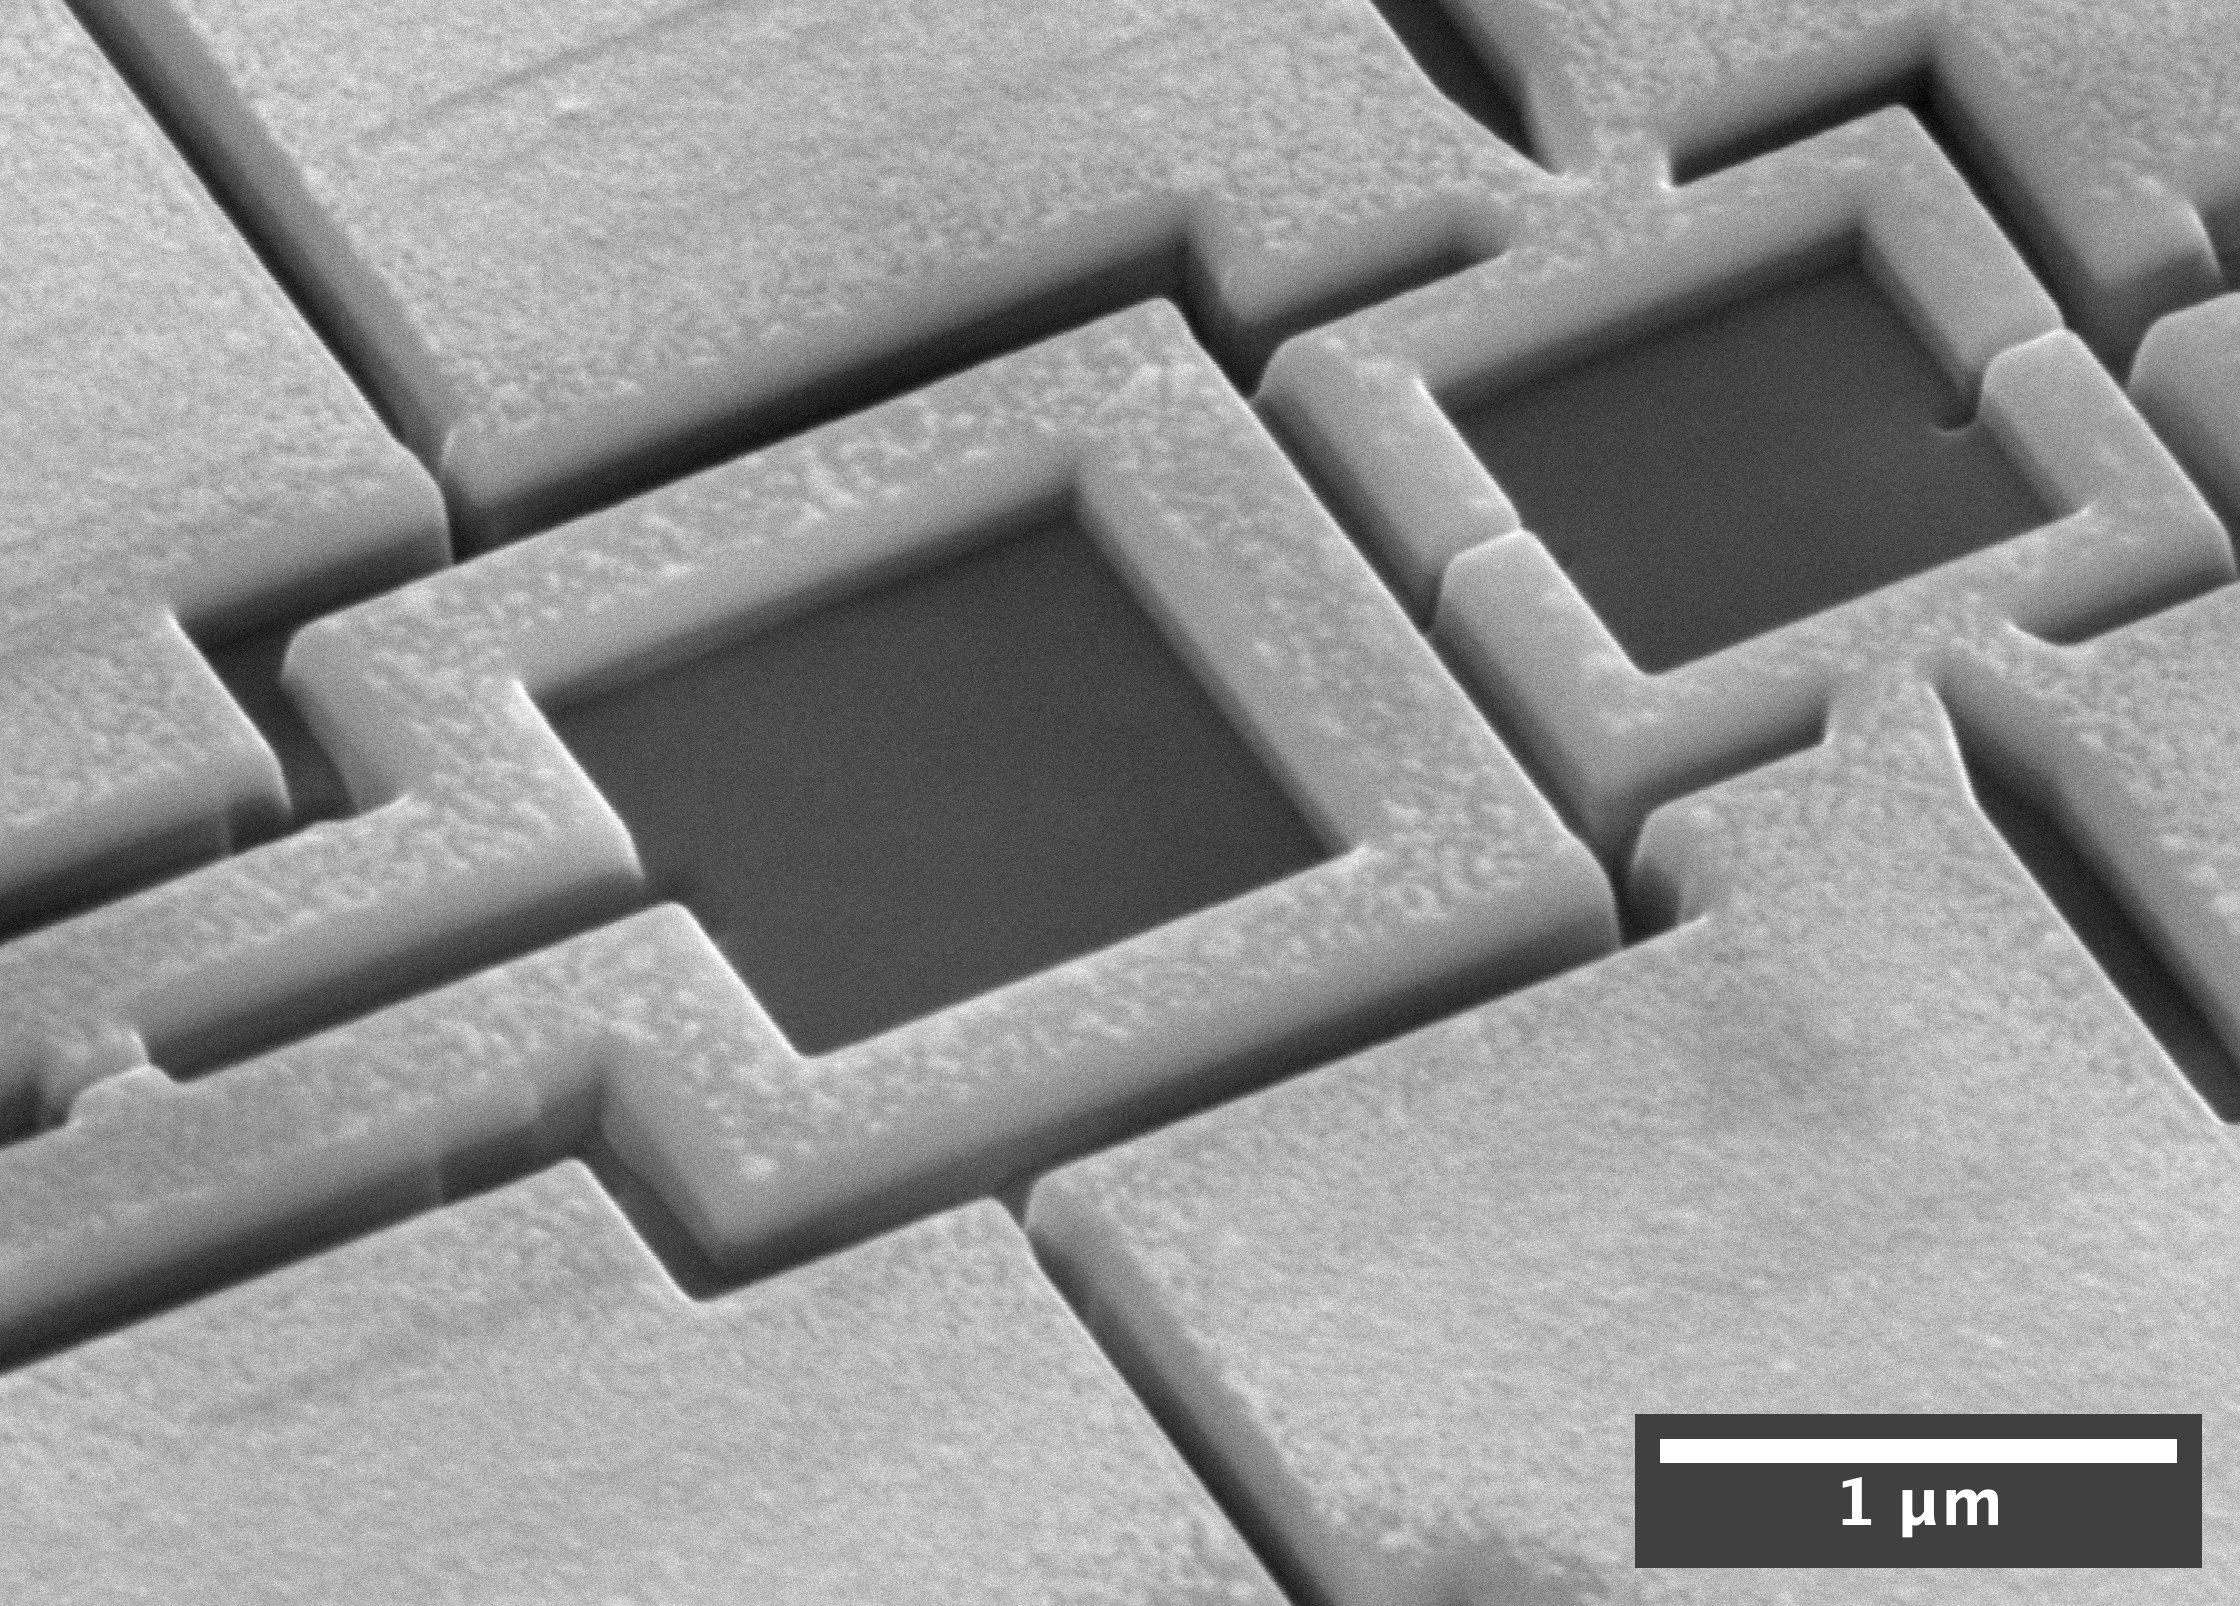
\includegraphics[width=\textwidth]{figures/samples/CP2/CP2.6B_SEM_overview.jpg}
		\subcaption{Overview of the device. The top loop shows the dc-SQUID and the bottom is the junction loop.}
	\end{subfigure}
	\hfill
	\begin{subfigure}[t]{0.3\textwidth}
		\centering
		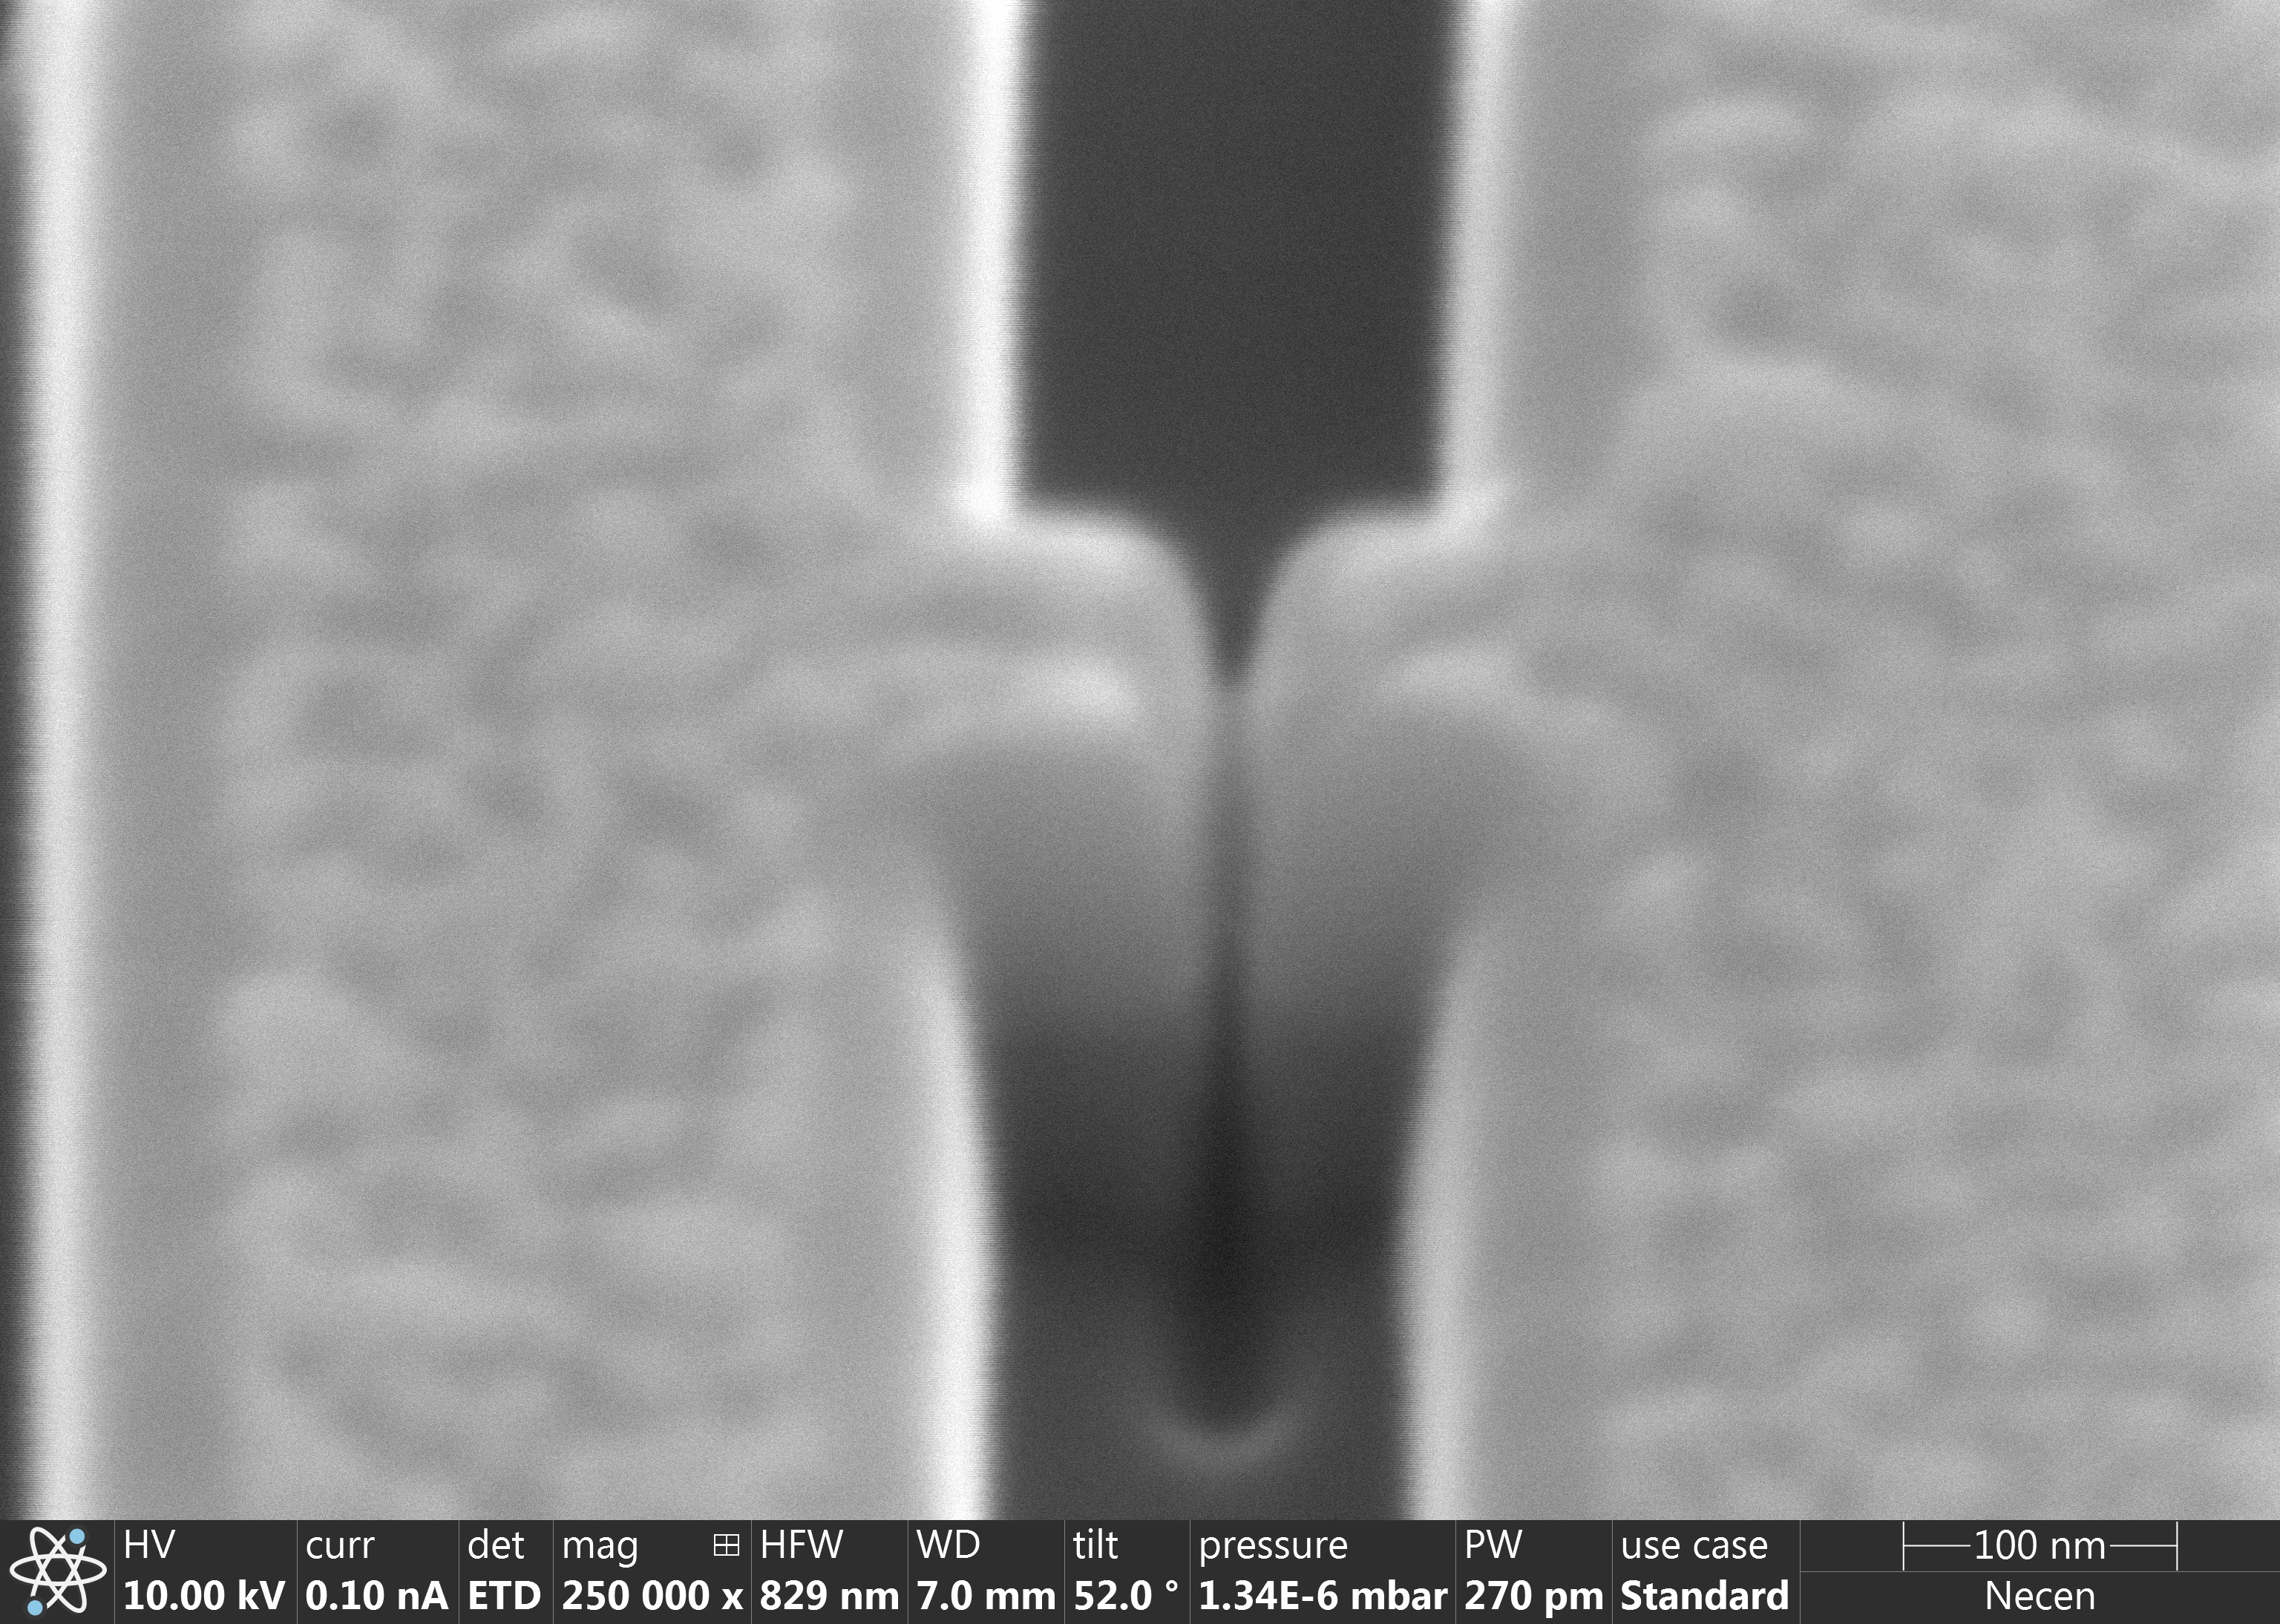
\includegraphics[width=\textwidth]{figures/samples/CP2/CP2.6B_SEM_junction.jpg}
		\subcaption{Zoomed in view of the junction, the width of the junction is \qty{12}{\nano\meter}.}
	\end{subfigure}
	\hfill
	\begin{subfigure}[t]{0.3\textwidth}
		\centering
		\includegraphics[width=\textwidth]{figures/samples/CP2/CP2.6B_SEM_SQUID.jpg}
		\subcaption{Zoomed in view of the dc-SQUID. The width of the junctions is \qty{22}{\nano\meter}.}
	\end{subfigure}

	\caption{Fine structures of sample CP2.6B after the FIB. See Table~\ref{tab:CP2.6B-geometries} for the exact geometries of the sample.}
	\label{fig:CP2.6B-SEM-images}
\end{figure}

\begin{table}
	\begin{subtable}{.5\linewidth}
		\centering
		\begin{tabular}{@{}lrr@{}}
			\toprule
			Parameter & Value \\ \midrule
			Junction loop $\diameter_{\text{outer}}$ & \qty{1.9}{\micro\meter} \\
			Junction loop $\diameter_{\text{inner}}$ & \qty{1.2}{\micro\meter} \\
			dc-SQUID $\diameter_{\text{outer}}$ & \qty{1.6}{\micro\meter} \\
			dc-SQUID $\diameter_{\text{inner}}$ & \qty{1.1}{\micro\meter} \\
			spacing & \qty{0.1}{\micro\meter} \\
			$d_{\ce{Cu}}$ & \qty{25}{\nano\meter} \\
			$d_{\ce{Nb}}$ & \qty{70}{\nano\meter} \\
			$d_{\ce{Au}}$ & \qty{7}{\nano\meter} \\
			\bottomrule
		\end{tabular}
    \end{subtable}
    \begin{subtable}{.5\linewidth}
    	\centering
    	\begin{tabular}{@{}lrr@{}}
    		\toprule
    		Parameter & Value \\ \midrule
    		$L_{l}$ & \qty{3.0}{\pico\henry} \\
			$L_{s}$ & \qty{3.0}{\pico\henry} \\
			$M$ & \qty{-0.2}{\pico\henry} \\
			$\delta$ & \num{0.001} \\
			$\kappa$ & \num{-0.058} \\
    		\bottomrule
    	\end{tabular}
    \end{subtable}
    \caption{The \textbf{left} table provides an overview of the geometries of CP2.6B as determined by SEM imaging and sputtering rates. The \textbf{right} table gives an overview of parameters found using a simulation based on the geometries. The geometries are based on sample CP1.2H.}
    \label{tab:CP2.6B-geometries}
\end{table}

\subsection{Results and discussion}
% !TEX root = ../../../thesis.tex
Figure~\ref{fig:CP2.6B_RT_curves} shows the RT-curves for the junction loop and dc-SQUID. The critical temperature for the bulk of the sample is lower (\qty{7}{\kelvin}) compared to the first sample (\qty{8}{\kelvin}). This can be explained by the proximity effect due to the interface between the \ce{Cu} and \ce{Nb}.\cite{cirilloSuperconductingProximityEffect2005} The longer `tail' is characteristic for SNS junctions as the normal metal slowly proximises.

\begin{figure}[ht!]
	\centering
	%% Creator: Matplotlib, PGF backend
%%
%% To include the figure in your LaTeX document, write
%%   \input{<filename>.pgf}
%%
%% Make sure the required packages are loaded in your preamble
%%   \usepackage{pgf}
%%
%% Also ensure that all the required font packages are loaded; for instance,
%% the lmodern package is sometimes necessary when using math font.
%%   \usepackage{lmodern}
%%
%% Figures using additional raster images can only be included by \input if
%% they are in the same directory as the main LaTeX file. For loading figures
%% from other directories you can use the `import` package
%%   \usepackage{import}
%%
%% and then include the figures with
%%   \import{<path to file>}{<filename>.pgf}
%%
%% Matplotlib used the following preamble
%%   \usepackage{siunitx}
%%   \usepackage{fontspec}
%%   \setmainfont{Times New Roman.ttf}[Path=\detokenize{/System/Library/Fonts/Supplemental/}]
%%   \setsansfont{DejaVuSans.ttf}[Path=\detokenize{/Users/julian/UL-BRP-analysis/venv/lib/python3.10/site-packages/matplotlib/mpl-data/fonts/ttf/}]
%%   \setmonofont{DejaVuSansMono.ttf}[Path=\detokenize{/Users/julian/UL-BRP-analysis/venv/lib/python3.10/site-packages/matplotlib/mpl-data/fonts/ttf/}]
%%   \makeatletter\@ifpackageloaded{underscore}{}{\usepackage[strings]{underscore}}\makeatother
%%
\begingroup%
\makeatletter%
\begin{pgfpicture}%
\pgfpathrectangle{\pgfpointorigin}{\pgfqpoint{3.025582in}{2.228467in}}%
\pgfusepath{use as bounding box, clip}%
\begin{pgfscope}%
\pgfsetbuttcap%
\pgfsetmiterjoin%
\definecolor{currentfill}{rgb}{1.000000,1.000000,1.000000}%
\pgfsetfillcolor{currentfill}%
\pgfsetlinewidth{0.000000pt}%
\definecolor{currentstroke}{rgb}{1.000000,1.000000,1.000000}%
\pgfsetstrokecolor{currentstroke}%
\pgfsetdash{}{0pt}%
\pgfpathmoveto{\pgfqpoint{0.000000in}{0.000000in}}%
\pgfpathlineto{\pgfqpoint{3.025582in}{0.000000in}}%
\pgfpathlineto{\pgfqpoint{3.025582in}{2.228467in}}%
\pgfpathlineto{\pgfqpoint{0.000000in}{2.228467in}}%
\pgfpathlineto{\pgfqpoint{0.000000in}{0.000000in}}%
\pgfpathclose%
\pgfusepath{fill}%
\end{pgfscope}%
\begin{pgfscope}%
\pgfsetbuttcap%
\pgfsetmiterjoin%
\definecolor{currentfill}{rgb}{1.000000,1.000000,1.000000}%
\pgfsetfillcolor{currentfill}%
\pgfsetlinewidth{0.000000pt}%
\definecolor{currentstroke}{rgb}{0.000000,0.000000,0.000000}%
\pgfsetstrokecolor{currentstroke}%
\pgfsetstrokeopacity{0.000000}%
\pgfsetdash{}{0pt}%
\pgfpathmoveto{\pgfqpoint{0.374978in}{0.431673in}}%
\pgfpathlineto{\pgfqpoint{2.975582in}{0.431673in}}%
\pgfpathlineto{\pgfqpoint{2.975582in}{2.178467in}}%
\pgfpathlineto{\pgfqpoint{0.374978in}{2.178467in}}%
\pgfpathlineto{\pgfqpoint{0.374978in}{0.431673in}}%
\pgfpathclose%
\pgfusepath{fill}%
\end{pgfscope}%
\begin{pgfscope}%
\pgfpathrectangle{\pgfqpoint{0.374978in}{0.431673in}}{\pgfqpoint{2.600604in}{1.746794in}}%
\pgfusepath{clip}%
\pgfsetbuttcap%
\pgfsetroundjoin%
\definecolor{currentfill}{rgb}{0.047059,0.364706,0.647059}%
\pgfsetfillcolor{currentfill}%
\pgfsetlinewidth{1.003750pt}%
\definecolor{currentstroke}{rgb}{0.047059,0.364706,0.647059}%
\pgfsetstrokecolor{currentstroke}%
\pgfsetdash{}{0pt}%
\pgfsys@defobject{currentmarker}{\pgfqpoint{-0.009821in}{-0.009821in}}{\pgfqpoint{0.009821in}{0.009821in}}{%
\pgfpathmoveto{\pgfqpoint{0.000000in}{-0.009821in}}%
\pgfpathcurveto{\pgfqpoint{0.002605in}{-0.009821in}}{\pgfqpoint{0.005103in}{-0.008786in}}{\pgfqpoint{0.006944in}{-0.006944in}}%
\pgfpathcurveto{\pgfqpoint{0.008786in}{-0.005103in}}{\pgfqpoint{0.009821in}{-0.002605in}}{\pgfqpoint{0.009821in}{0.000000in}}%
\pgfpathcurveto{\pgfqpoint{0.009821in}{0.002605in}}{\pgfqpoint{0.008786in}{0.005103in}}{\pgfqpoint{0.006944in}{0.006944in}}%
\pgfpathcurveto{\pgfqpoint{0.005103in}{0.008786in}}{\pgfqpoint{0.002605in}{0.009821in}}{\pgfqpoint{0.000000in}{0.009821in}}%
\pgfpathcurveto{\pgfqpoint{-0.002605in}{0.009821in}}{\pgfqpoint{-0.005103in}{0.008786in}}{\pgfqpoint{-0.006944in}{0.006944in}}%
\pgfpathcurveto{\pgfqpoint{-0.008786in}{0.005103in}}{\pgfqpoint{-0.009821in}{0.002605in}}{\pgfqpoint{-0.009821in}{0.000000in}}%
\pgfpathcurveto{\pgfqpoint{-0.009821in}{-0.002605in}}{\pgfqpoint{-0.008786in}{-0.005103in}}{\pgfqpoint{-0.006944in}{-0.006944in}}%
\pgfpathcurveto{\pgfqpoint{-0.005103in}{-0.008786in}}{\pgfqpoint{-0.002605in}{-0.009821in}}{\pgfqpoint{0.000000in}{-0.009821in}}%
\pgfpathlineto{\pgfqpoint{0.000000in}{-0.009821in}}%
\pgfpathclose%
\pgfusepath{stroke,fill}%
}%
\begin{pgfscope}%
\pgfsys@transformshift{0.374978in}{0.431658in}%
\pgfsys@useobject{currentmarker}{}%
\end{pgfscope}%
\begin{pgfscope}%
\pgfsys@transformshift{0.449281in}{0.431661in}%
\pgfsys@useobject{currentmarker}{}%
\end{pgfscope}%
\begin{pgfscope}%
\pgfsys@transformshift{0.523547in}{0.431552in}%
\pgfsys@useobject{currentmarker}{}%
\end{pgfscope}%
\begin{pgfscope}%
\pgfsys@transformshift{0.597962in}{0.431598in}%
\pgfsys@useobject{currentmarker}{}%
\end{pgfscope}%
\begin{pgfscope}%
\pgfsys@transformshift{0.672302in}{0.431793in}%
\pgfsys@useobject{currentmarker}{}%
\end{pgfscope}%
\begin{pgfscope}%
\pgfsys@transformshift{0.746456in}{0.431579in}%
\pgfsys@useobject{currentmarker}{}%
\end{pgfscope}%
\begin{pgfscope}%
\pgfsys@transformshift{0.820796in}{0.431544in}%
\pgfsys@useobject{currentmarker}{}%
\end{pgfscope}%
\begin{pgfscope}%
\pgfsys@transformshift{0.895062in}{0.431538in}%
\pgfsys@useobject{currentmarker}{}%
\end{pgfscope}%
\begin{pgfscope}%
\pgfsys@transformshift{0.969402in}{0.431776in}%
\pgfsys@useobject{currentmarker}{}%
\end{pgfscope}%
\begin{pgfscope}%
\pgfsys@transformshift{1.043854in}{0.431825in}%
\pgfsys@useobject{currentmarker}{}%
\end{pgfscope}%
\begin{pgfscope}%
\pgfsys@transformshift{1.118082in}{0.431804in}%
\pgfsys@useobject{currentmarker}{}%
\end{pgfscope}%
\begin{pgfscope}%
\pgfsys@transformshift{1.192311in}{0.431663in}%
\pgfsys@useobject{currentmarker}{}%
\end{pgfscope}%
\begin{pgfscope}%
\pgfsys@transformshift{1.266503in}{0.431478in}%
\pgfsys@useobject{currentmarker}{}%
\end{pgfscope}%
\begin{pgfscope}%
\pgfsys@transformshift{1.340917in}{0.431820in}%
\pgfsys@useobject{currentmarker}{}%
\end{pgfscope}%
\begin{pgfscope}%
\pgfsys@transformshift{1.415146in}{0.431701in}%
\pgfsys@useobject{currentmarker}{}%
\end{pgfscope}%
\begin{pgfscope}%
\pgfsys@transformshift{1.489486in}{0.431564in}%
\pgfsys@useobject{currentmarker}{}%
\end{pgfscope}%
\begin{pgfscope}%
\pgfsys@transformshift{1.563714in}{0.431433in}%
\pgfsys@useobject{currentmarker}{}%
\end{pgfscope}%
\begin{pgfscope}%
\pgfsys@transformshift{1.638092in}{0.431853in}%
\pgfsys@useobject{currentmarker}{}%
\end{pgfscope}%
\begin{pgfscope}%
\pgfsys@transformshift{1.712320in}{0.431116in}%
\pgfsys@useobject{currentmarker}{}%
\end{pgfscope}%
\begin{pgfscope}%
\pgfsys@transformshift{1.786772in}{0.431981in}%
\pgfsys@useobject{currentmarker}{}%
\end{pgfscope}%
\begin{pgfscope}%
\pgfsys@transformshift{1.861001in}{0.431837in}%
\pgfsys@useobject{currentmarker}{}%
\end{pgfscope}%
\begin{pgfscope}%
\pgfsys@transformshift{1.935267in}{0.431757in}%
\pgfsys@useobject{currentmarker}{}%
\end{pgfscope}%
\begin{pgfscope}%
\pgfsys@transformshift{2.009607in}{0.431067in}%
\pgfsys@useobject{currentmarker}{}%
\end{pgfscope}%
\begin{pgfscope}%
\pgfsys@transformshift{2.084095in}{0.437887in}%
\pgfsys@useobject{currentmarker}{}%
\end{pgfscope}%
\begin{pgfscope}%
\pgfsys@transformshift{2.158138in}{0.554625in}%
\pgfsys@useobject{currentmarker}{}%
\end{pgfscope}%
\begin{pgfscope}%
\pgfsys@transformshift{2.232590in}{1.046198in}%
\pgfsys@useobject{currentmarker}{}%
\end{pgfscope}%
\begin{pgfscope}%
\pgfsys@transformshift{2.306633in}{1.821806in}%
\pgfsys@useobject{currentmarker}{}%
\end{pgfscope}%
\begin{pgfscope}%
\pgfsys@transformshift{2.381122in}{2.051163in}%
\pgfsys@useobject{currentmarker}{}%
\end{pgfscope}%
\begin{pgfscope}%
\pgfsys@transformshift{2.455350in}{2.078089in}%
\pgfsys@useobject{currentmarker}{}%
\end{pgfscope}%
\begin{pgfscope}%
\pgfsys@transformshift{2.529690in}{2.083097in}%
\pgfsys@useobject{currentmarker}{}%
\end{pgfscope}%
\begin{pgfscope}%
\pgfsys@transformshift{2.604142in}{2.089250in}%
\pgfsys@useobject{currentmarker}{}%
\end{pgfscope}%
\begin{pgfscope}%
\pgfsys@transformshift{2.678296in}{2.080044in}%
\pgfsys@useobject{currentmarker}{}%
\end{pgfscope}%
\begin{pgfscope}%
\pgfsys@transformshift{2.752674in}{2.082042in}%
\pgfsys@useobject{currentmarker}{}%
\end{pgfscope}%
\begin{pgfscope}%
\pgfsys@transformshift{2.826902in}{2.078803in}%
\pgfsys@useobject{currentmarker}{}%
\end{pgfscope}%
\begin{pgfscope}%
\pgfsys@transformshift{2.901168in}{2.084315in}%
\pgfsys@useobject{currentmarker}{}%
\end{pgfscope}%
\begin{pgfscope}%
\pgfsys@transformshift{2.975508in}{2.081726in}%
\pgfsys@useobject{currentmarker}{}%
\end{pgfscope}%
\begin{pgfscope}%
\pgfsys@transformshift{3.049811in}{2.080572in}%
\pgfsys@useobject{currentmarker}{}%
\end{pgfscope}%
\begin{pgfscope}%
\pgfsys@transformshift{3.124151in}{2.082062in}%
\pgfsys@useobject{currentmarker}{}%
\end{pgfscope}%
\begin{pgfscope}%
\pgfsys@transformshift{3.198529in}{2.080931in}%
\pgfsys@useobject{currentmarker}{}%
\end{pgfscope}%
\begin{pgfscope}%
\pgfsys@transformshift{3.272794in}{2.079132in}%
\pgfsys@useobject{currentmarker}{}%
\end{pgfscope}%
\begin{pgfscope}%
\pgfsys@transformshift{3.347134in}{2.081911in}%
\pgfsys@useobject{currentmarker}{}%
\end{pgfscope}%
\end{pgfscope}%
\begin{pgfscope}%
\pgfpathrectangle{\pgfqpoint{0.374978in}{0.431673in}}{\pgfqpoint{2.600604in}{1.746794in}}%
\pgfusepath{clip}%
\pgfsetbuttcap%
\pgfsetroundjoin%
\definecolor{currentfill}{rgb}{0.000000,0.725490,0.270588}%
\pgfsetfillcolor{currentfill}%
\pgfsetlinewidth{1.003750pt}%
\definecolor{currentstroke}{rgb}{0.000000,0.725490,0.270588}%
\pgfsetstrokecolor{currentstroke}%
\pgfsetdash{}{0pt}%
\pgfsys@defobject{currentmarker}{\pgfqpoint{-0.009821in}{-0.009821in}}{\pgfqpoint{0.009821in}{0.009821in}}{%
\pgfpathmoveto{\pgfqpoint{0.000000in}{-0.009821in}}%
\pgfpathcurveto{\pgfqpoint{0.002605in}{-0.009821in}}{\pgfqpoint{0.005103in}{-0.008786in}}{\pgfqpoint{0.006944in}{-0.006944in}}%
\pgfpathcurveto{\pgfqpoint{0.008786in}{-0.005103in}}{\pgfqpoint{0.009821in}{-0.002605in}}{\pgfqpoint{0.009821in}{0.000000in}}%
\pgfpathcurveto{\pgfqpoint{0.009821in}{0.002605in}}{\pgfqpoint{0.008786in}{0.005103in}}{\pgfqpoint{0.006944in}{0.006944in}}%
\pgfpathcurveto{\pgfqpoint{0.005103in}{0.008786in}}{\pgfqpoint{0.002605in}{0.009821in}}{\pgfqpoint{0.000000in}{0.009821in}}%
\pgfpathcurveto{\pgfqpoint{-0.002605in}{0.009821in}}{\pgfqpoint{-0.005103in}{0.008786in}}{\pgfqpoint{-0.006944in}{0.006944in}}%
\pgfpathcurveto{\pgfqpoint{-0.008786in}{0.005103in}}{\pgfqpoint{-0.009821in}{0.002605in}}{\pgfqpoint{-0.009821in}{0.000000in}}%
\pgfpathcurveto{\pgfqpoint{-0.009821in}{-0.002605in}}{\pgfqpoint{-0.008786in}{-0.005103in}}{\pgfqpoint{-0.006944in}{-0.006944in}}%
\pgfpathcurveto{\pgfqpoint{-0.005103in}{-0.008786in}}{\pgfqpoint{-0.002605in}{-0.009821in}}{\pgfqpoint{0.000000in}{-0.009821in}}%
\pgfpathlineto{\pgfqpoint{0.000000in}{-0.009821in}}%
\pgfpathclose%
\pgfusepath{stroke,fill}%
}%
\begin{pgfscope}%
\pgfsys@transformshift{111.086337in}{2.087202in}%
\pgfsys@useobject{currentmarker}{}%
\end{pgfscope}%
\begin{pgfscope}%
\pgfsys@transformshift{109.266880in}{2.071562in}%
\pgfsys@useobject{currentmarker}{}%
\end{pgfscope}%
\begin{pgfscope}%
\pgfsys@transformshift{107.405553in}{2.069637in}%
\pgfsys@useobject{currentmarker}{}%
\end{pgfscope}%
\begin{pgfscope}%
\pgfsys@transformshift{105.549390in}{2.063154in}%
\pgfsys@useobject{currentmarker}{}%
\end{pgfscope}%
\begin{pgfscope}%
\pgfsys@transformshift{103.692968in}{2.051145in}%
\pgfsys@useobject{currentmarker}{}%
\end{pgfscope}%
\begin{pgfscope}%
\pgfsys@transformshift{101.840669in}{2.040701in}%
\pgfsys@useobject{currentmarker}{}%
\end{pgfscope}%
\begin{pgfscope}%
\pgfsys@transformshift{99.981608in}{2.030643in}%
\pgfsys@useobject{currentmarker}{}%
\end{pgfscope}%
\begin{pgfscope}%
\pgfsys@transformshift{98.127972in}{2.019558in}%
\pgfsys@useobject{currentmarker}{}%
\end{pgfscope}%
\begin{pgfscope}%
\pgfsys@transformshift{96.273110in}{2.006569in}%
\pgfsys@useobject{currentmarker}{}%
\end{pgfscope}%
\begin{pgfscope}%
\pgfsys@transformshift{94.416204in}{1.996116in}%
\pgfsys@useobject{currentmarker}{}%
\end{pgfscope}%
\begin{pgfscope}%
\pgfsys@transformshift{92.559596in}{1.984924in}%
\pgfsys@useobject{currentmarker}{}%
\end{pgfscope}%
\begin{pgfscope}%
\pgfsys@transformshift{90.700572in}{1.972648in}%
\pgfsys@useobject{currentmarker}{}%
\end{pgfscope}%
\begin{pgfscope}%
\pgfsys@transformshift{88.843481in}{1.961013in}%
\pgfsys@useobject{currentmarker}{}%
\end{pgfscope}%
\begin{pgfscope}%
\pgfsys@transformshift{86.986501in}{1.948235in}%
\pgfsys@useobject{currentmarker}{}%
\end{pgfscope}%
\begin{pgfscope}%
\pgfsys@transformshift{85.132047in}{1.937838in}%
\pgfsys@useobject{currentmarker}{}%
\end{pgfscope}%
\begin{pgfscope}%
\pgfsys@transformshift{83.274882in}{1.925211in}%
\pgfsys@useobject{currentmarker}{}%
\end{pgfscope}%
\begin{pgfscope}%
\pgfsys@transformshift{81.421691in}{1.911111in}%
\pgfsys@useobject{currentmarker}{}%
\end{pgfscope}%
\begin{pgfscope}%
\pgfsys@transformshift{79.562334in}{1.899817in}%
\pgfsys@useobject{currentmarker}{}%
\end{pgfscope}%
\begin{pgfscope}%
\pgfsys@transformshift{77.706245in}{1.889980in}%
\pgfsys@useobject{currentmarker}{}%
\end{pgfscope}%
\begin{pgfscope}%
\pgfsys@transformshift{75.852535in}{1.877749in}%
\pgfsys@useobject{currentmarker}{}%
\end{pgfscope}%
\begin{pgfscope}%
\pgfsys@transformshift{73.996521in}{1.864456in}%
\pgfsys@useobject{currentmarker}{}%
\end{pgfscope}%
\begin{pgfscope}%
\pgfsys@transformshift{72.140061in}{1.852941in}%
\pgfsys@useobject{currentmarker}{}%
\end{pgfscope}%
\begin{pgfscope}%
\pgfsys@transformshift{70.280740in}{1.839224in}%
\pgfsys@useobject{currentmarker}{}%
\end{pgfscope}%
\begin{pgfscope}%
\pgfsys@transformshift{68.427475in}{1.829438in}%
\pgfsys@useobject{currentmarker}{}%
\end{pgfscope}%
\begin{pgfscope}%
\pgfsys@transformshift{66.570235in}{1.817405in}%
\pgfsys@useobject{currentmarker}{}%
\end{pgfscope}%
\begin{pgfscope}%
\pgfsys@transformshift{64.711658in}{1.805490in}%
\pgfsys@useobject{currentmarker}{}%
\end{pgfscope}%
\begin{pgfscope}%
\pgfsys@transformshift{62.855830in}{1.791707in}%
\pgfsys@useobject{currentmarker}{}%
\end{pgfscope}%
\begin{pgfscope}%
\pgfsys@transformshift{60.998441in}{1.780248in}%
\pgfsys@useobject{currentmarker}{}%
\end{pgfscope}%
\begin{pgfscope}%
\pgfsys@transformshift{59.142873in}{1.767082in}%
\pgfsys@useobject{currentmarker}{}%
\end{pgfscope}%
\begin{pgfscope}%
\pgfsys@transformshift{57.287973in}{1.755004in}%
\pgfsys@useobject{currentmarker}{}%
\end{pgfscope}%
\begin{pgfscope}%
\pgfsys@transformshift{55.432294in}{1.743136in}%
\pgfsys@useobject{currentmarker}{}%
\end{pgfscope}%
\begin{pgfscope}%
\pgfsys@transformshift{53.576206in}{1.730205in}%
\pgfsys@useobject{currentmarker}{}%
\end{pgfscope}%
\begin{pgfscope}%
\pgfsys@transformshift{51.716291in}{1.716878in}%
\pgfsys@useobject{currentmarker}{}%
\end{pgfscope}%
\begin{pgfscope}%
\pgfsys@transformshift{49.860054in}{1.706119in}%
\pgfsys@useobject{currentmarker}{}%
\end{pgfscope}%
\begin{pgfscope}%
\pgfsys@transformshift{48.002331in}{1.691249in}%
\pgfsys@useobject{currentmarker}{}%
\end{pgfscope}%
\begin{pgfscope}%
\pgfsys@transformshift{46.147320in}{1.678632in}%
\pgfsys@useobject{currentmarker}{}%
\end{pgfscope}%
\begin{pgfscope}%
\pgfsys@transformshift{44.289300in}{1.665117in}%
\pgfsys@useobject{currentmarker}{}%
\end{pgfscope}%
\begin{pgfscope}%
\pgfsys@transformshift{42.430128in}{1.651253in}%
\pgfsys@useobject{currentmarker}{}%
\end{pgfscope}%
\begin{pgfscope}%
\pgfsys@transformshift{40.571847in}{1.638719in}%
\pgfsys@useobject{currentmarker}{}%
\end{pgfscope}%
\begin{pgfscope}%
\pgfsys@transformshift{38.714385in}{1.624292in}%
\pgfsys@useobject{currentmarker}{}%
\end{pgfscope}%
\begin{pgfscope}%
\pgfsys@transformshift{36.857033in}{1.610228in}%
\pgfsys@useobject{currentmarker}{}%
\end{pgfscope}%
\begin{pgfscope}%
\pgfsys@transformshift{34.994778in}{1.597590in}%
\pgfsys@useobject{currentmarker}{}%
\end{pgfscope}%
\begin{pgfscope}%
\pgfsys@transformshift{33.135383in}{1.582252in}%
\pgfsys@useobject{currentmarker}{}%
\end{pgfscope}%
\begin{pgfscope}%
\pgfsys@transformshift{31.275988in}{1.567814in}%
\pgfsys@useobject{currentmarker}{}%
\end{pgfscope}%
\begin{pgfscope}%
\pgfsys@transformshift{29.422835in}{1.556028in}%
\pgfsys@useobject{currentmarker}{}%
\end{pgfscope}%
\begin{pgfscope}%
\pgfsys@transformshift{27.564592in}{1.538623in}%
\pgfsys@useobject{currentmarker}{}%
\end{pgfscope}%
\begin{pgfscope}%
\pgfsys@transformshift{25.709172in}{1.526416in}%
\pgfsys@useobject{currentmarker}{}%
\end{pgfscope}%
\begin{pgfscope}%
\pgfsys@transformshift{23.851152in}{1.513648in}%
\pgfsys@useobject{currentmarker}{}%
\end{pgfscope}%
\begin{pgfscope}%
\pgfsys@transformshift{21.997924in}{1.498228in}%
\pgfsys@useobject{currentmarker}{}%
\end{pgfscope}%
\begin{pgfscope}%
\pgfsys@transformshift{20.140647in}{1.483382in}%
\pgfsys@useobject{currentmarker}{}%
\end{pgfscope}%
\begin{pgfscope}%
\pgfsys@transformshift{18.269512in}{1.468499in}%
\pgfsys@useobject{currentmarker}{}%
\end{pgfscope}%
\begin{pgfscope}%
\pgfsys@transformshift{16.405548in}{1.459552in}%
\pgfsys@useobject{currentmarker}{}%
\end{pgfscope}%
\begin{pgfscope}%
\pgfsys@transformshift{14.486897in}{1.447345in}%
\pgfsys@useobject{currentmarker}{}%
\end{pgfscope}%
\begin{pgfscope}%
\pgfsys@transformshift{12.629954in}{1.439893in}%
\pgfsys@useobject{currentmarker}{}%
\end{pgfscope}%
\begin{pgfscope}%
\pgfsys@transformshift{10.774534in}{1.433574in}%
\pgfsys@useobject{currentmarker}{}%
\end{pgfscope}%
\begin{pgfscope}%
\pgfsys@transformshift{8.918557in}{1.428037in}%
\pgfsys@useobject{currentmarker}{}%
\end{pgfscope}%
\begin{pgfscope}%
\pgfsys@transformshift{7.061614in}{1.432255in}%
\pgfsys@useobject{currentmarker}{}%
\end{pgfscope}%
\begin{pgfscope}%
\pgfsys@transformshift{5.203854in}{1.426775in}%
\pgfsys@useobject{currentmarker}{}%
\end{pgfscope}%
\begin{pgfscope}%
\pgfsys@transformshift{3.347134in}{1.423552in}%
\pgfsys@useobject{currentmarker}{}%
\end{pgfscope}%
\begin{pgfscope}%
\pgfsys@transformshift{3.718501in}{1.420243in}%
\pgfsys@useobject{currentmarker}{}%
\end{pgfscope}%
\begin{pgfscope}%
\pgfsys@transformshift{3.681386in}{1.420404in}%
\pgfsys@useobject{currentmarker}{}%
\end{pgfscope}%
\begin{pgfscope}%
\pgfsys@transformshift{3.644309in}{1.420402in}%
\pgfsys@useobject{currentmarker}{}%
\end{pgfscope}%
\begin{pgfscope}%
\pgfsys@transformshift{3.607009in}{1.420505in}%
\pgfsys@useobject{currentmarker}{}%
\end{pgfscope}%
\begin{pgfscope}%
\pgfsys@transformshift{3.569969in}{1.420244in}%
\pgfsys@useobject{currentmarker}{}%
\end{pgfscope}%
\begin{pgfscope}%
\pgfsys@transformshift{3.532855in}{1.420441in}%
\pgfsys@useobject{currentmarker}{}%
\end{pgfscope}%
\begin{pgfscope}%
\pgfsys@transformshift{3.495592in}{1.420111in}%
\pgfsys@useobject{currentmarker}{}%
\end{pgfscope}%
\begin{pgfscope}%
\pgfsys@transformshift{3.458589in}{1.420562in}%
\pgfsys@useobject{currentmarker}{}%
\end{pgfscope}%
\begin{pgfscope}%
\pgfsys@transformshift{3.421363in}{1.420272in}%
\pgfsys@useobject{currentmarker}{}%
\end{pgfscope}%
\begin{pgfscope}%
\pgfsys@transformshift{3.384286in}{1.420463in}%
\pgfsys@useobject{currentmarker}{}%
\end{pgfscope}%
\begin{pgfscope}%
\pgfsys@transformshift{3.347134in}{1.420116in}%
\pgfsys@useobject{currentmarker}{}%
\end{pgfscope}%
\begin{pgfscope}%
\pgfsys@transformshift{3.310243in}{1.420520in}%
\pgfsys@useobject{currentmarker}{}%
\end{pgfscope}%
\begin{pgfscope}%
\pgfsys@transformshift{3.269748in}{1.420307in}%
\pgfsys@useobject{currentmarker}{}%
\end{pgfscope}%
\begin{pgfscope}%
\pgfsys@transformshift{3.235606in}{1.420451in}%
\pgfsys@useobject{currentmarker}{}%
\end{pgfscope}%
\begin{pgfscope}%
\pgfsys@transformshift{3.198417in}{1.420687in}%
\pgfsys@useobject{currentmarker}{}%
\end{pgfscope}%
\begin{pgfscope}%
\pgfsys@transformshift{3.161266in}{1.420358in}%
\pgfsys@useobject{currentmarker}{}%
\end{pgfscope}%
\begin{pgfscope}%
\pgfsys@transformshift{3.124077in}{1.420112in}%
\pgfsys@useobject{currentmarker}{}%
\end{pgfscope}%
\begin{pgfscope}%
\pgfsys@transformshift{3.086331in}{1.420110in}%
\pgfsys@useobject{currentmarker}{}%
\end{pgfscope}%
\begin{pgfscope}%
\pgfsys@transformshift{3.047619in}{1.419956in}%
\pgfsys@useobject{currentmarker}{}%
\end{pgfscope}%
\begin{pgfscope}%
\pgfsys@transformshift{3.013328in}{1.420438in}%
\pgfsys@useobject{currentmarker}{}%
\end{pgfscope}%
\begin{pgfscope}%
\pgfsys@transformshift{2.976028in}{1.420210in}%
\pgfsys@useobject{currentmarker}{}%
\end{pgfscope}%
\begin{pgfscope}%
\pgfsys@transformshift{2.938505in}{1.420059in}%
\pgfsys@useobject{currentmarker}{}%
\end{pgfscope}%
\begin{pgfscope}%
\pgfsys@transformshift{2.901019in}{1.419980in}%
\pgfsys@useobject{currentmarker}{}%
\end{pgfscope}%
\begin{pgfscope}%
\pgfsys@transformshift{2.864054in}{1.420388in}%
\pgfsys@useobject{currentmarker}{}%
\end{pgfscope}%
\begin{pgfscope}%
\pgfsys@transformshift{2.826791in}{1.420298in}%
\pgfsys@useobject{currentmarker}{}%
\end{pgfscope}%
\begin{pgfscope}%
\pgfsys@transformshift{2.789676in}{1.420424in}%
\pgfsys@useobject{currentmarker}{}%
\end{pgfscope}%
\begin{pgfscope}%
\pgfsys@transformshift{2.752599in}{1.420280in}%
\pgfsys@useobject{currentmarker}{}%
\end{pgfscope}%
\begin{pgfscope}%
\pgfsys@transformshift{2.715559in}{1.419957in}%
\pgfsys@useobject{currentmarker}{}%
\end{pgfscope}%
\begin{pgfscope}%
\pgfsys@transformshift{2.678259in}{1.419973in}%
\pgfsys@useobject{currentmarker}{}%
\end{pgfscope}%
\begin{pgfscope}%
\pgfsys@transformshift{2.641070in}{1.419930in}%
\pgfsys@useobject{currentmarker}{}%
\end{pgfscope}%
\begin{pgfscope}%
\pgfsys@transformshift{2.603956in}{1.419626in}%
\pgfsys@useobject{currentmarker}{}%
\end{pgfscope}%
\begin{pgfscope}%
\pgfsys@transformshift{2.566805in}{1.419981in}%
\pgfsys@useobject{currentmarker}{}%
\end{pgfscope}%
\begin{pgfscope}%
\pgfsys@transformshift{2.529802in}{1.419899in}%
\pgfsys@useobject{currentmarker}{}%
\end{pgfscope}%
\begin{pgfscope}%
\pgfsys@transformshift{2.492465in}{1.420207in}%
\pgfsys@useobject{currentmarker}{}%
\end{pgfscope}%
\begin{pgfscope}%
\pgfsys@transformshift{2.455276in}{1.421310in}%
\pgfsys@useobject{currentmarker}{}%
\end{pgfscope}%
\begin{pgfscope}%
\pgfsys@transformshift{2.418236in}{1.421772in}%
\pgfsys@useobject{currentmarker}{}%
\end{pgfscope}%
\begin{pgfscope}%
\pgfsys@transformshift{2.381010in}{1.421100in}%
\pgfsys@useobject{currentmarker}{}%
\end{pgfscope}%
\begin{pgfscope}%
\pgfsys@transformshift{2.343933in}{1.420685in}%
\pgfsys@useobject{currentmarker}{}%
\end{pgfscope}%
\begin{pgfscope}%
\pgfsys@transformshift{2.306707in}{1.420595in}%
\pgfsys@useobject{currentmarker}{}%
\end{pgfscope}%
\begin{pgfscope}%
\pgfsys@transformshift{2.269556in}{1.423132in}%
\pgfsys@useobject{currentmarker}{}%
\end{pgfscope}%
\begin{pgfscope}%
\pgfsys@transformshift{2.232553in}{1.436681in}%
\pgfsys@useobject{currentmarker}{}%
\end{pgfscope}%
\begin{pgfscope}%
\pgfsys@transformshift{2.195327in}{1.427531in}%
\pgfsys@useobject{currentmarker}{}%
\end{pgfscope}%
\begin{pgfscope}%
\pgfsys@transformshift{2.158175in}{1.385173in}%
\pgfsys@useobject{currentmarker}{}%
\end{pgfscope}%
\begin{pgfscope}%
\pgfsys@transformshift{2.121098in}{1.293130in}%
\pgfsys@useobject{currentmarker}{}%
\end{pgfscope}%
\begin{pgfscope}%
\pgfsys@transformshift{2.083835in}{1.167531in}%
\pgfsys@useobject{currentmarker}{}%
\end{pgfscope}%
\begin{pgfscope}%
\pgfsys@transformshift{2.046832in}{1.025714in}%
\pgfsys@useobject{currentmarker}{}%
\end{pgfscope}%
\begin{pgfscope}%
\pgfsys@transformshift{2.009718in}{0.889546in}%
\pgfsys@useobject{currentmarker}{}%
\end{pgfscope}%
\begin{pgfscope}%
\pgfsys@transformshift{1.972492in}{0.794484in}%
\pgfsys@useobject{currentmarker}{}%
\end{pgfscope}%
\begin{pgfscope}%
\pgfsys@transformshift{1.935341in}{0.719450in}%
\pgfsys@useobject{currentmarker}{}%
\end{pgfscope}%
\begin{pgfscope}%
\pgfsys@transformshift{1.898226in}{0.666223in}%
\pgfsys@useobject{currentmarker}{}%
\end{pgfscope}%
\begin{pgfscope}%
\pgfsys@transformshift{1.860889in}{0.627766in}%
\pgfsys@useobject{currentmarker}{}%
\end{pgfscope}%
\begin{pgfscope}%
\pgfsys@transformshift{1.823849in}{0.598863in}%
\pgfsys@useobject{currentmarker}{}%
\end{pgfscope}%
\begin{pgfscope}%
\pgfsys@transformshift{1.786549in}{0.577353in}%
\pgfsys@useobject{currentmarker}{}%
\end{pgfscope}%
\begin{pgfscope}%
\pgfsys@transformshift{1.749621in}{0.559653in}%
\pgfsys@useobject{currentmarker}{}%
\end{pgfscope}%
\begin{pgfscope}%
\pgfsys@transformshift{1.712358in}{0.547613in}%
\pgfsys@useobject{currentmarker}{}%
\end{pgfscope}%
\begin{pgfscope}%
\pgfsys@transformshift{1.675206in}{0.536435in}%
\pgfsys@useobject{currentmarker}{}%
\end{pgfscope}%
\begin{pgfscope}%
\pgfsys@transformshift{1.638055in}{0.526121in}%
\pgfsys@useobject{currentmarker}{}%
\end{pgfscope}%
\begin{pgfscope}%
\pgfsys@transformshift{1.600903in}{0.518073in}%
\pgfsys@useobject{currentmarker}{}%
\end{pgfscope}%
\begin{pgfscope}%
\pgfsys@transformshift{1.563900in}{0.510219in}%
\pgfsys@useobject{currentmarker}{}%
\end{pgfscope}%
\begin{pgfscope}%
\pgfsys@transformshift{1.526600in}{0.501200in}%
\pgfsys@useobject{currentmarker}{}%
\end{pgfscope}%
\begin{pgfscope}%
\pgfsys@transformshift{1.489412in}{0.494369in}%
\pgfsys@useobject{currentmarker}{}%
\end{pgfscope}%
\begin{pgfscope}%
\pgfsys@transformshift{1.452371in}{0.486499in}%
\pgfsys@useobject{currentmarker}{}%
\end{pgfscope}%
\begin{pgfscope}%
\pgfsys@transformshift{1.415406in}{0.479589in}%
\pgfsys@useobject{currentmarker}{}%
\end{pgfscope}%
\begin{pgfscope}%
\pgfsys@transformshift{1.378068in}{0.472851in}%
\pgfsys@useobject{currentmarker}{}%
\end{pgfscope}%
\begin{pgfscope}%
\pgfsys@transformshift{1.340917in}{0.466950in}%
\pgfsys@useobject{currentmarker}{}%
\end{pgfscope}%
\begin{pgfscope}%
\pgfsys@transformshift{1.303654in}{0.460768in}%
\pgfsys@useobject{currentmarker}{}%
\end{pgfscope}%
\begin{pgfscope}%
\pgfsys@transformshift{1.266540in}{0.455380in}%
\pgfsys@useobject{currentmarker}{}%
\end{pgfscope}%
\begin{pgfscope}%
\pgfsys@transformshift{1.229500in}{0.450846in}%
\pgfsys@useobject{currentmarker}{}%
\end{pgfscope}%
\begin{pgfscope}%
\pgfsys@transformshift{1.192237in}{0.446720in}%
\pgfsys@useobject{currentmarker}{}%
\end{pgfscope}%
\begin{pgfscope}%
\pgfsys@transformshift{1.155197in}{0.442878in}%
\pgfsys@useobject{currentmarker}{}%
\end{pgfscope}%
\begin{pgfscope}%
\pgfsys@transformshift{1.118008in}{0.440382in}%
\pgfsys@useobject{currentmarker}{}%
\end{pgfscope}%
\begin{pgfscope}%
\pgfsys@transformshift{1.081042in}{0.438306in}%
\pgfsys@useobject{currentmarker}{}%
\end{pgfscope}%
\begin{pgfscope}%
\pgfsys@transformshift{1.043779in}{0.436136in}%
\pgfsys@useobject{currentmarker}{}%
\end{pgfscope}%
\begin{pgfscope}%
\pgfsys@transformshift{1.006554in}{0.434768in}%
\pgfsys@useobject{currentmarker}{}%
\end{pgfscope}%
\begin{pgfscope}%
\pgfsys@transformshift{0.969514in}{0.433725in}%
\pgfsys@useobject{currentmarker}{}%
\end{pgfscope}%
\begin{pgfscope}%
\pgfsys@transformshift{0.932213in}{0.433121in}%
\pgfsys@useobject{currentmarker}{}%
\end{pgfscope}%
\begin{pgfscope}%
\pgfsys@transformshift{0.895062in}{0.432691in}%
\pgfsys@useobject{currentmarker}{}%
\end{pgfscope}%
\begin{pgfscope}%
\pgfsys@transformshift{0.857985in}{0.432344in}%
\pgfsys@useobject{currentmarker}{}%
\end{pgfscope}%
\begin{pgfscope}%
\pgfsys@transformshift{0.820870in}{0.431974in}%
\pgfsys@useobject{currentmarker}{}%
\end{pgfscope}%
\begin{pgfscope}%
\pgfsys@transformshift{0.783570in}{0.432056in}%
\pgfsys@useobject{currentmarker}{}%
\end{pgfscope}%
\begin{pgfscope}%
\pgfsys@transformshift{0.746530in}{0.431850in}%
\pgfsys@useobject{currentmarker}{}%
\end{pgfscope}%
\begin{pgfscope}%
\pgfsys@transformshift{0.709267in}{0.431735in}%
\pgfsys@useobject{currentmarker}{}%
\end{pgfscope}%
\begin{pgfscope}%
\pgfsys@transformshift{0.672227in}{0.431787in}%
\pgfsys@useobject{currentmarker}{}%
\end{pgfscope}%
\begin{pgfscope}%
\pgfsys@transformshift{0.634964in}{0.431875in}%
\pgfsys@useobject{currentmarker}{}%
\end{pgfscope}%
\begin{pgfscope}%
\pgfsys@transformshift{0.597924in}{0.431667in}%
\pgfsys@useobject{currentmarker}{}%
\end{pgfscope}%
\begin{pgfscope}%
\pgfsys@transformshift{0.560773in}{0.431587in}%
\pgfsys@useobject{currentmarker}{}%
\end{pgfscope}%
\begin{pgfscope}%
\pgfsys@transformshift{0.523584in}{0.431729in}%
\pgfsys@useobject{currentmarker}{}%
\end{pgfscope}%
\begin{pgfscope}%
\pgfsys@transformshift{0.486544in}{0.431703in}%
\pgfsys@useobject{currentmarker}{}%
\end{pgfscope}%
\begin{pgfscope}%
\pgfsys@transformshift{0.449281in}{0.431770in}%
\pgfsys@useobject{currentmarker}{}%
\end{pgfscope}%
\begin{pgfscope}%
\pgfsys@transformshift{0.412130in}{0.431687in}%
\pgfsys@useobject{currentmarker}{}%
\end{pgfscope}%
\begin{pgfscope}%
\pgfsys@transformshift{0.374978in}{0.431598in}%
\pgfsys@useobject{currentmarker}{}%
\end{pgfscope}%
\end{pgfscope}%
\begin{pgfscope}%
\pgfsetbuttcap%
\pgfsetroundjoin%
\definecolor{currentfill}{rgb}{0.000000,0.000000,0.000000}%
\pgfsetfillcolor{currentfill}%
\pgfsetlinewidth{0.501875pt}%
\definecolor{currentstroke}{rgb}{0.000000,0.000000,0.000000}%
\pgfsetstrokecolor{currentstroke}%
\pgfsetdash{}{0pt}%
\pgfsys@defobject{currentmarker}{\pgfqpoint{0.000000in}{0.000000in}}{\pgfqpoint{0.000000in}{0.041667in}}{%
\pgfpathmoveto{\pgfqpoint{0.000000in}{0.000000in}}%
\pgfpathlineto{\pgfqpoint{0.000000in}{0.041667in}}%
\pgfusepath{stroke,fill}%
}%
\begin{pgfscope}%
\pgfsys@transformshift{0.374978in}{0.431673in}%
\pgfsys@useobject{currentmarker}{}%
\end{pgfscope}%
\end{pgfscope}%
\begin{pgfscope}%
\pgfsetbuttcap%
\pgfsetroundjoin%
\definecolor{currentfill}{rgb}{0.000000,0.000000,0.000000}%
\pgfsetfillcolor{currentfill}%
\pgfsetlinewidth{0.501875pt}%
\definecolor{currentstroke}{rgb}{0.000000,0.000000,0.000000}%
\pgfsetstrokecolor{currentstroke}%
\pgfsetdash{}{0pt}%
\pgfsys@defobject{currentmarker}{\pgfqpoint{0.000000in}{-0.041667in}}{\pgfqpoint{0.000000in}{0.000000in}}{%
\pgfpathmoveto{\pgfqpoint{0.000000in}{0.000000in}}%
\pgfpathlineto{\pgfqpoint{0.000000in}{-0.041667in}}%
\pgfusepath{stroke,fill}%
}%
\begin{pgfscope}%
\pgfsys@transformshift{0.374978in}{2.178467in}%
\pgfsys@useobject{currentmarker}{}%
\end{pgfscope}%
\end{pgfscope}%
\begin{pgfscope}%
\definecolor{textcolor}{rgb}{0.000000,0.000000,0.000000}%
\pgfsetstrokecolor{textcolor}%
\pgfsetfillcolor{textcolor}%
\pgftext[x=0.374978in,y=0.383062in,,top]{\color{textcolor}\rmfamily\fontsize{10.000000}{12.000000}\selectfont \(\displaystyle {2}\)}%
\end{pgfscope}%
\begin{pgfscope}%
\pgfsetbuttcap%
\pgfsetroundjoin%
\definecolor{currentfill}{rgb}{0.000000,0.000000,0.000000}%
\pgfsetfillcolor{currentfill}%
\pgfsetlinewidth{0.501875pt}%
\definecolor{currentstroke}{rgb}{0.000000,0.000000,0.000000}%
\pgfsetstrokecolor{currentstroke}%
\pgfsetdash{}{0pt}%
\pgfsys@defobject{currentmarker}{\pgfqpoint{0.000000in}{0.000000in}}{\pgfqpoint{0.000000in}{0.041667in}}{%
\pgfpathmoveto{\pgfqpoint{0.000000in}{0.000000in}}%
\pgfpathlineto{\pgfqpoint{0.000000in}{0.041667in}}%
\pgfusepath{stroke,fill}%
}%
\begin{pgfscope}%
\pgfsys@transformshift{1.118008in}{0.431673in}%
\pgfsys@useobject{currentmarker}{}%
\end{pgfscope}%
\end{pgfscope}%
\begin{pgfscope}%
\pgfsetbuttcap%
\pgfsetroundjoin%
\definecolor{currentfill}{rgb}{0.000000,0.000000,0.000000}%
\pgfsetfillcolor{currentfill}%
\pgfsetlinewidth{0.501875pt}%
\definecolor{currentstroke}{rgb}{0.000000,0.000000,0.000000}%
\pgfsetstrokecolor{currentstroke}%
\pgfsetdash{}{0pt}%
\pgfsys@defobject{currentmarker}{\pgfqpoint{0.000000in}{-0.041667in}}{\pgfqpoint{0.000000in}{0.000000in}}{%
\pgfpathmoveto{\pgfqpoint{0.000000in}{0.000000in}}%
\pgfpathlineto{\pgfqpoint{0.000000in}{-0.041667in}}%
\pgfusepath{stroke,fill}%
}%
\begin{pgfscope}%
\pgfsys@transformshift{1.118008in}{2.178467in}%
\pgfsys@useobject{currentmarker}{}%
\end{pgfscope}%
\end{pgfscope}%
\begin{pgfscope}%
\definecolor{textcolor}{rgb}{0.000000,0.000000,0.000000}%
\pgfsetstrokecolor{textcolor}%
\pgfsetfillcolor{textcolor}%
\pgftext[x=1.118008in,y=0.383062in,,top]{\color{textcolor}\rmfamily\fontsize{10.000000}{12.000000}\selectfont \(\displaystyle {4}\)}%
\end{pgfscope}%
\begin{pgfscope}%
\pgfsetbuttcap%
\pgfsetroundjoin%
\definecolor{currentfill}{rgb}{0.000000,0.000000,0.000000}%
\pgfsetfillcolor{currentfill}%
\pgfsetlinewidth{0.501875pt}%
\definecolor{currentstroke}{rgb}{0.000000,0.000000,0.000000}%
\pgfsetstrokecolor{currentstroke}%
\pgfsetdash{}{0pt}%
\pgfsys@defobject{currentmarker}{\pgfqpoint{0.000000in}{0.000000in}}{\pgfqpoint{0.000000in}{0.041667in}}{%
\pgfpathmoveto{\pgfqpoint{0.000000in}{0.000000in}}%
\pgfpathlineto{\pgfqpoint{0.000000in}{0.041667in}}%
\pgfusepath{stroke,fill}%
}%
\begin{pgfscope}%
\pgfsys@transformshift{1.861038in}{0.431673in}%
\pgfsys@useobject{currentmarker}{}%
\end{pgfscope}%
\end{pgfscope}%
\begin{pgfscope}%
\pgfsetbuttcap%
\pgfsetroundjoin%
\definecolor{currentfill}{rgb}{0.000000,0.000000,0.000000}%
\pgfsetfillcolor{currentfill}%
\pgfsetlinewidth{0.501875pt}%
\definecolor{currentstroke}{rgb}{0.000000,0.000000,0.000000}%
\pgfsetstrokecolor{currentstroke}%
\pgfsetdash{}{0pt}%
\pgfsys@defobject{currentmarker}{\pgfqpoint{0.000000in}{-0.041667in}}{\pgfqpoint{0.000000in}{0.000000in}}{%
\pgfpathmoveto{\pgfqpoint{0.000000in}{0.000000in}}%
\pgfpathlineto{\pgfqpoint{0.000000in}{-0.041667in}}%
\pgfusepath{stroke,fill}%
}%
\begin{pgfscope}%
\pgfsys@transformshift{1.861038in}{2.178467in}%
\pgfsys@useobject{currentmarker}{}%
\end{pgfscope}%
\end{pgfscope}%
\begin{pgfscope}%
\definecolor{textcolor}{rgb}{0.000000,0.000000,0.000000}%
\pgfsetstrokecolor{textcolor}%
\pgfsetfillcolor{textcolor}%
\pgftext[x=1.861038in,y=0.383062in,,top]{\color{textcolor}\rmfamily\fontsize{10.000000}{12.000000}\selectfont \(\displaystyle {6}\)}%
\end{pgfscope}%
\begin{pgfscope}%
\pgfsetbuttcap%
\pgfsetroundjoin%
\definecolor{currentfill}{rgb}{0.000000,0.000000,0.000000}%
\pgfsetfillcolor{currentfill}%
\pgfsetlinewidth{0.501875pt}%
\definecolor{currentstroke}{rgb}{0.000000,0.000000,0.000000}%
\pgfsetstrokecolor{currentstroke}%
\pgfsetdash{}{0pt}%
\pgfsys@defobject{currentmarker}{\pgfqpoint{0.000000in}{0.000000in}}{\pgfqpoint{0.000000in}{0.041667in}}{%
\pgfpathmoveto{\pgfqpoint{0.000000in}{0.000000in}}%
\pgfpathlineto{\pgfqpoint{0.000000in}{0.041667in}}%
\pgfusepath{stroke,fill}%
}%
\begin{pgfscope}%
\pgfsys@transformshift{2.604068in}{0.431673in}%
\pgfsys@useobject{currentmarker}{}%
\end{pgfscope}%
\end{pgfscope}%
\begin{pgfscope}%
\pgfsetbuttcap%
\pgfsetroundjoin%
\definecolor{currentfill}{rgb}{0.000000,0.000000,0.000000}%
\pgfsetfillcolor{currentfill}%
\pgfsetlinewidth{0.501875pt}%
\definecolor{currentstroke}{rgb}{0.000000,0.000000,0.000000}%
\pgfsetstrokecolor{currentstroke}%
\pgfsetdash{}{0pt}%
\pgfsys@defobject{currentmarker}{\pgfqpoint{0.000000in}{-0.041667in}}{\pgfqpoint{0.000000in}{0.000000in}}{%
\pgfpathmoveto{\pgfqpoint{0.000000in}{0.000000in}}%
\pgfpathlineto{\pgfqpoint{0.000000in}{-0.041667in}}%
\pgfusepath{stroke,fill}%
}%
\begin{pgfscope}%
\pgfsys@transformshift{2.604068in}{2.178467in}%
\pgfsys@useobject{currentmarker}{}%
\end{pgfscope}%
\end{pgfscope}%
\begin{pgfscope}%
\definecolor{textcolor}{rgb}{0.000000,0.000000,0.000000}%
\pgfsetstrokecolor{textcolor}%
\pgfsetfillcolor{textcolor}%
\pgftext[x=2.604068in,y=0.383062in,,top]{\color{textcolor}\rmfamily\fontsize{10.000000}{12.000000}\selectfont \(\displaystyle {8}\)}%
\end{pgfscope}%
\begin{pgfscope}%
\pgfsetbuttcap%
\pgfsetroundjoin%
\definecolor{currentfill}{rgb}{0.000000,0.000000,0.000000}%
\pgfsetfillcolor{currentfill}%
\pgfsetlinewidth{0.501875pt}%
\definecolor{currentstroke}{rgb}{0.000000,0.000000,0.000000}%
\pgfsetstrokecolor{currentstroke}%
\pgfsetdash{}{0pt}%
\pgfsys@defobject{currentmarker}{\pgfqpoint{0.000000in}{0.000000in}}{\pgfqpoint{0.000000in}{0.020833in}}{%
\pgfpathmoveto{\pgfqpoint{0.000000in}{0.000000in}}%
\pgfpathlineto{\pgfqpoint{0.000000in}{0.020833in}}%
\pgfusepath{stroke,fill}%
}%
\begin{pgfscope}%
\pgfsys@transformshift{0.560736in}{0.431673in}%
\pgfsys@useobject{currentmarker}{}%
\end{pgfscope}%
\end{pgfscope}%
\begin{pgfscope}%
\pgfsetbuttcap%
\pgfsetroundjoin%
\definecolor{currentfill}{rgb}{0.000000,0.000000,0.000000}%
\pgfsetfillcolor{currentfill}%
\pgfsetlinewidth{0.501875pt}%
\definecolor{currentstroke}{rgb}{0.000000,0.000000,0.000000}%
\pgfsetstrokecolor{currentstroke}%
\pgfsetdash{}{0pt}%
\pgfsys@defobject{currentmarker}{\pgfqpoint{0.000000in}{-0.020833in}}{\pgfqpoint{0.000000in}{0.000000in}}{%
\pgfpathmoveto{\pgfqpoint{0.000000in}{0.000000in}}%
\pgfpathlineto{\pgfqpoint{0.000000in}{-0.020833in}}%
\pgfusepath{stroke,fill}%
}%
\begin{pgfscope}%
\pgfsys@transformshift{0.560736in}{2.178467in}%
\pgfsys@useobject{currentmarker}{}%
\end{pgfscope}%
\end{pgfscope}%
\begin{pgfscope}%
\pgfsetbuttcap%
\pgfsetroundjoin%
\definecolor{currentfill}{rgb}{0.000000,0.000000,0.000000}%
\pgfsetfillcolor{currentfill}%
\pgfsetlinewidth{0.501875pt}%
\definecolor{currentstroke}{rgb}{0.000000,0.000000,0.000000}%
\pgfsetstrokecolor{currentstroke}%
\pgfsetdash{}{0pt}%
\pgfsys@defobject{currentmarker}{\pgfqpoint{0.000000in}{0.000000in}}{\pgfqpoint{0.000000in}{0.020833in}}{%
\pgfpathmoveto{\pgfqpoint{0.000000in}{0.000000in}}%
\pgfpathlineto{\pgfqpoint{0.000000in}{0.020833in}}%
\pgfusepath{stroke,fill}%
}%
\begin{pgfscope}%
\pgfsys@transformshift{0.746493in}{0.431673in}%
\pgfsys@useobject{currentmarker}{}%
\end{pgfscope}%
\end{pgfscope}%
\begin{pgfscope}%
\pgfsetbuttcap%
\pgfsetroundjoin%
\definecolor{currentfill}{rgb}{0.000000,0.000000,0.000000}%
\pgfsetfillcolor{currentfill}%
\pgfsetlinewidth{0.501875pt}%
\definecolor{currentstroke}{rgb}{0.000000,0.000000,0.000000}%
\pgfsetstrokecolor{currentstroke}%
\pgfsetdash{}{0pt}%
\pgfsys@defobject{currentmarker}{\pgfqpoint{0.000000in}{-0.020833in}}{\pgfqpoint{0.000000in}{0.000000in}}{%
\pgfpathmoveto{\pgfqpoint{0.000000in}{0.000000in}}%
\pgfpathlineto{\pgfqpoint{0.000000in}{-0.020833in}}%
\pgfusepath{stroke,fill}%
}%
\begin{pgfscope}%
\pgfsys@transformshift{0.746493in}{2.178467in}%
\pgfsys@useobject{currentmarker}{}%
\end{pgfscope}%
\end{pgfscope}%
\begin{pgfscope}%
\pgfsetbuttcap%
\pgfsetroundjoin%
\definecolor{currentfill}{rgb}{0.000000,0.000000,0.000000}%
\pgfsetfillcolor{currentfill}%
\pgfsetlinewidth{0.501875pt}%
\definecolor{currentstroke}{rgb}{0.000000,0.000000,0.000000}%
\pgfsetstrokecolor{currentstroke}%
\pgfsetdash{}{0pt}%
\pgfsys@defobject{currentmarker}{\pgfqpoint{0.000000in}{0.000000in}}{\pgfqpoint{0.000000in}{0.020833in}}{%
\pgfpathmoveto{\pgfqpoint{0.000000in}{0.000000in}}%
\pgfpathlineto{\pgfqpoint{0.000000in}{0.020833in}}%
\pgfusepath{stroke,fill}%
}%
\begin{pgfscope}%
\pgfsys@transformshift{0.932251in}{0.431673in}%
\pgfsys@useobject{currentmarker}{}%
\end{pgfscope}%
\end{pgfscope}%
\begin{pgfscope}%
\pgfsetbuttcap%
\pgfsetroundjoin%
\definecolor{currentfill}{rgb}{0.000000,0.000000,0.000000}%
\pgfsetfillcolor{currentfill}%
\pgfsetlinewidth{0.501875pt}%
\definecolor{currentstroke}{rgb}{0.000000,0.000000,0.000000}%
\pgfsetstrokecolor{currentstroke}%
\pgfsetdash{}{0pt}%
\pgfsys@defobject{currentmarker}{\pgfqpoint{0.000000in}{-0.020833in}}{\pgfqpoint{0.000000in}{0.000000in}}{%
\pgfpathmoveto{\pgfqpoint{0.000000in}{0.000000in}}%
\pgfpathlineto{\pgfqpoint{0.000000in}{-0.020833in}}%
\pgfusepath{stroke,fill}%
}%
\begin{pgfscope}%
\pgfsys@transformshift{0.932251in}{2.178467in}%
\pgfsys@useobject{currentmarker}{}%
\end{pgfscope}%
\end{pgfscope}%
\begin{pgfscope}%
\pgfsetbuttcap%
\pgfsetroundjoin%
\definecolor{currentfill}{rgb}{0.000000,0.000000,0.000000}%
\pgfsetfillcolor{currentfill}%
\pgfsetlinewidth{0.501875pt}%
\definecolor{currentstroke}{rgb}{0.000000,0.000000,0.000000}%
\pgfsetstrokecolor{currentstroke}%
\pgfsetdash{}{0pt}%
\pgfsys@defobject{currentmarker}{\pgfqpoint{0.000000in}{0.000000in}}{\pgfqpoint{0.000000in}{0.020833in}}{%
\pgfpathmoveto{\pgfqpoint{0.000000in}{0.000000in}}%
\pgfpathlineto{\pgfqpoint{0.000000in}{0.020833in}}%
\pgfusepath{stroke,fill}%
}%
\begin{pgfscope}%
\pgfsys@transformshift{1.303766in}{0.431673in}%
\pgfsys@useobject{currentmarker}{}%
\end{pgfscope}%
\end{pgfscope}%
\begin{pgfscope}%
\pgfsetbuttcap%
\pgfsetroundjoin%
\definecolor{currentfill}{rgb}{0.000000,0.000000,0.000000}%
\pgfsetfillcolor{currentfill}%
\pgfsetlinewidth{0.501875pt}%
\definecolor{currentstroke}{rgb}{0.000000,0.000000,0.000000}%
\pgfsetstrokecolor{currentstroke}%
\pgfsetdash{}{0pt}%
\pgfsys@defobject{currentmarker}{\pgfqpoint{0.000000in}{-0.020833in}}{\pgfqpoint{0.000000in}{0.000000in}}{%
\pgfpathmoveto{\pgfqpoint{0.000000in}{0.000000in}}%
\pgfpathlineto{\pgfqpoint{0.000000in}{-0.020833in}}%
\pgfusepath{stroke,fill}%
}%
\begin{pgfscope}%
\pgfsys@transformshift{1.303766in}{2.178467in}%
\pgfsys@useobject{currentmarker}{}%
\end{pgfscope}%
\end{pgfscope}%
\begin{pgfscope}%
\pgfsetbuttcap%
\pgfsetroundjoin%
\definecolor{currentfill}{rgb}{0.000000,0.000000,0.000000}%
\pgfsetfillcolor{currentfill}%
\pgfsetlinewidth{0.501875pt}%
\definecolor{currentstroke}{rgb}{0.000000,0.000000,0.000000}%
\pgfsetstrokecolor{currentstroke}%
\pgfsetdash{}{0pt}%
\pgfsys@defobject{currentmarker}{\pgfqpoint{0.000000in}{0.000000in}}{\pgfqpoint{0.000000in}{0.020833in}}{%
\pgfpathmoveto{\pgfqpoint{0.000000in}{0.000000in}}%
\pgfpathlineto{\pgfqpoint{0.000000in}{0.020833in}}%
\pgfusepath{stroke,fill}%
}%
\begin{pgfscope}%
\pgfsys@transformshift{1.489523in}{0.431673in}%
\pgfsys@useobject{currentmarker}{}%
\end{pgfscope}%
\end{pgfscope}%
\begin{pgfscope}%
\pgfsetbuttcap%
\pgfsetroundjoin%
\definecolor{currentfill}{rgb}{0.000000,0.000000,0.000000}%
\pgfsetfillcolor{currentfill}%
\pgfsetlinewidth{0.501875pt}%
\definecolor{currentstroke}{rgb}{0.000000,0.000000,0.000000}%
\pgfsetstrokecolor{currentstroke}%
\pgfsetdash{}{0pt}%
\pgfsys@defobject{currentmarker}{\pgfqpoint{0.000000in}{-0.020833in}}{\pgfqpoint{0.000000in}{0.000000in}}{%
\pgfpathmoveto{\pgfqpoint{0.000000in}{0.000000in}}%
\pgfpathlineto{\pgfqpoint{0.000000in}{-0.020833in}}%
\pgfusepath{stroke,fill}%
}%
\begin{pgfscope}%
\pgfsys@transformshift{1.489523in}{2.178467in}%
\pgfsys@useobject{currentmarker}{}%
\end{pgfscope}%
\end{pgfscope}%
\begin{pgfscope}%
\pgfsetbuttcap%
\pgfsetroundjoin%
\definecolor{currentfill}{rgb}{0.000000,0.000000,0.000000}%
\pgfsetfillcolor{currentfill}%
\pgfsetlinewidth{0.501875pt}%
\definecolor{currentstroke}{rgb}{0.000000,0.000000,0.000000}%
\pgfsetstrokecolor{currentstroke}%
\pgfsetdash{}{0pt}%
\pgfsys@defobject{currentmarker}{\pgfqpoint{0.000000in}{0.000000in}}{\pgfqpoint{0.000000in}{0.020833in}}{%
\pgfpathmoveto{\pgfqpoint{0.000000in}{0.000000in}}%
\pgfpathlineto{\pgfqpoint{0.000000in}{0.020833in}}%
\pgfusepath{stroke,fill}%
}%
\begin{pgfscope}%
\pgfsys@transformshift{1.675280in}{0.431673in}%
\pgfsys@useobject{currentmarker}{}%
\end{pgfscope}%
\end{pgfscope}%
\begin{pgfscope}%
\pgfsetbuttcap%
\pgfsetroundjoin%
\definecolor{currentfill}{rgb}{0.000000,0.000000,0.000000}%
\pgfsetfillcolor{currentfill}%
\pgfsetlinewidth{0.501875pt}%
\definecolor{currentstroke}{rgb}{0.000000,0.000000,0.000000}%
\pgfsetstrokecolor{currentstroke}%
\pgfsetdash{}{0pt}%
\pgfsys@defobject{currentmarker}{\pgfqpoint{0.000000in}{-0.020833in}}{\pgfqpoint{0.000000in}{0.000000in}}{%
\pgfpathmoveto{\pgfqpoint{0.000000in}{0.000000in}}%
\pgfpathlineto{\pgfqpoint{0.000000in}{-0.020833in}}%
\pgfusepath{stroke,fill}%
}%
\begin{pgfscope}%
\pgfsys@transformshift{1.675280in}{2.178467in}%
\pgfsys@useobject{currentmarker}{}%
\end{pgfscope}%
\end{pgfscope}%
\begin{pgfscope}%
\pgfsetbuttcap%
\pgfsetroundjoin%
\definecolor{currentfill}{rgb}{0.000000,0.000000,0.000000}%
\pgfsetfillcolor{currentfill}%
\pgfsetlinewidth{0.501875pt}%
\definecolor{currentstroke}{rgb}{0.000000,0.000000,0.000000}%
\pgfsetstrokecolor{currentstroke}%
\pgfsetdash{}{0pt}%
\pgfsys@defobject{currentmarker}{\pgfqpoint{0.000000in}{0.000000in}}{\pgfqpoint{0.000000in}{0.020833in}}{%
\pgfpathmoveto{\pgfqpoint{0.000000in}{0.000000in}}%
\pgfpathlineto{\pgfqpoint{0.000000in}{0.020833in}}%
\pgfusepath{stroke,fill}%
}%
\begin{pgfscope}%
\pgfsys@transformshift{2.046795in}{0.431673in}%
\pgfsys@useobject{currentmarker}{}%
\end{pgfscope}%
\end{pgfscope}%
\begin{pgfscope}%
\pgfsetbuttcap%
\pgfsetroundjoin%
\definecolor{currentfill}{rgb}{0.000000,0.000000,0.000000}%
\pgfsetfillcolor{currentfill}%
\pgfsetlinewidth{0.501875pt}%
\definecolor{currentstroke}{rgb}{0.000000,0.000000,0.000000}%
\pgfsetstrokecolor{currentstroke}%
\pgfsetdash{}{0pt}%
\pgfsys@defobject{currentmarker}{\pgfqpoint{0.000000in}{-0.020833in}}{\pgfqpoint{0.000000in}{0.000000in}}{%
\pgfpathmoveto{\pgfqpoint{0.000000in}{0.000000in}}%
\pgfpathlineto{\pgfqpoint{0.000000in}{-0.020833in}}%
\pgfusepath{stroke,fill}%
}%
\begin{pgfscope}%
\pgfsys@transformshift{2.046795in}{2.178467in}%
\pgfsys@useobject{currentmarker}{}%
\end{pgfscope}%
\end{pgfscope}%
\begin{pgfscope}%
\pgfsetbuttcap%
\pgfsetroundjoin%
\definecolor{currentfill}{rgb}{0.000000,0.000000,0.000000}%
\pgfsetfillcolor{currentfill}%
\pgfsetlinewidth{0.501875pt}%
\definecolor{currentstroke}{rgb}{0.000000,0.000000,0.000000}%
\pgfsetstrokecolor{currentstroke}%
\pgfsetdash{}{0pt}%
\pgfsys@defobject{currentmarker}{\pgfqpoint{0.000000in}{0.000000in}}{\pgfqpoint{0.000000in}{0.020833in}}{%
\pgfpathmoveto{\pgfqpoint{0.000000in}{0.000000in}}%
\pgfpathlineto{\pgfqpoint{0.000000in}{0.020833in}}%
\pgfusepath{stroke,fill}%
}%
\begin{pgfscope}%
\pgfsys@transformshift{2.232553in}{0.431673in}%
\pgfsys@useobject{currentmarker}{}%
\end{pgfscope}%
\end{pgfscope}%
\begin{pgfscope}%
\pgfsetbuttcap%
\pgfsetroundjoin%
\definecolor{currentfill}{rgb}{0.000000,0.000000,0.000000}%
\pgfsetfillcolor{currentfill}%
\pgfsetlinewidth{0.501875pt}%
\definecolor{currentstroke}{rgb}{0.000000,0.000000,0.000000}%
\pgfsetstrokecolor{currentstroke}%
\pgfsetdash{}{0pt}%
\pgfsys@defobject{currentmarker}{\pgfqpoint{0.000000in}{-0.020833in}}{\pgfqpoint{0.000000in}{0.000000in}}{%
\pgfpathmoveto{\pgfqpoint{0.000000in}{0.000000in}}%
\pgfpathlineto{\pgfqpoint{0.000000in}{-0.020833in}}%
\pgfusepath{stroke,fill}%
}%
\begin{pgfscope}%
\pgfsys@transformshift{2.232553in}{2.178467in}%
\pgfsys@useobject{currentmarker}{}%
\end{pgfscope}%
\end{pgfscope}%
\begin{pgfscope}%
\pgfsetbuttcap%
\pgfsetroundjoin%
\definecolor{currentfill}{rgb}{0.000000,0.000000,0.000000}%
\pgfsetfillcolor{currentfill}%
\pgfsetlinewidth{0.501875pt}%
\definecolor{currentstroke}{rgb}{0.000000,0.000000,0.000000}%
\pgfsetstrokecolor{currentstroke}%
\pgfsetdash{}{0pt}%
\pgfsys@defobject{currentmarker}{\pgfqpoint{0.000000in}{0.000000in}}{\pgfqpoint{0.000000in}{0.020833in}}{%
\pgfpathmoveto{\pgfqpoint{0.000000in}{0.000000in}}%
\pgfpathlineto{\pgfqpoint{0.000000in}{0.020833in}}%
\pgfusepath{stroke,fill}%
}%
\begin{pgfscope}%
\pgfsys@transformshift{2.418310in}{0.431673in}%
\pgfsys@useobject{currentmarker}{}%
\end{pgfscope}%
\end{pgfscope}%
\begin{pgfscope}%
\pgfsetbuttcap%
\pgfsetroundjoin%
\definecolor{currentfill}{rgb}{0.000000,0.000000,0.000000}%
\pgfsetfillcolor{currentfill}%
\pgfsetlinewidth{0.501875pt}%
\definecolor{currentstroke}{rgb}{0.000000,0.000000,0.000000}%
\pgfsetstrokecolor{currentstroke}%
\pgfsetdash{}{0pt}%
\pgfsys@defobject{currentmarker}{\pgfqpoint{0.000000in}{-0.020833in}}{\pgfqpoint{0.000000in}{0.000000in}}{%
\pgfpathmoveto{\pgfqpoint{0.000000in}{0.000000in}}%
\pgfpathlineto{\pgfqpoint{0.000000in}{-0.020833in}}%
\pgfusepath{stroke,fill}%
}%
\begin{pgfscope}%
\pgfsys@transformshift{2.418310in}{2.178467in}%
\pgfsys@useobject{currentmarker}{}%
\end{pgfscope}%
\end{pgfscope}%
\begin{pgfscope}%
\pgfsetbuttcap%
\pgfsetroundjoin%
\definecolor{currentfill}{rgb}{0.000000,0.000000,0.000000}%
\pgfsetfillcolor{currentfill}%
\pgfsetlinewidth{0.501875pt}%
\definecolor{currentstroke}{rgb}{0.000000,0.000000,0.000000}%
\pgfsetstrokecolor{currentstroke}%
\pgfsetdash{}{0pt}%
\pgfsys@defobject{currentmarker}{\pgfqpoint{0.000000in}{0.000000in}}{\pgfqpoint{0.000000in}{0.020833in}}{%
\pgfpathmoveto{\pgfqpoint{0.000000in}{0.000000in}}%
\pgfpathlineto{\pgfqpoint{0.000000in}{0.020833in}}%
\pgfusepath{stroke,fill}%
}%
\begin{pgfscope}%
\pgfsys@transformshift{2.789825in}{0.431673in}%
\pgfsys@useobject{currentmarker}{}%
\end{pgfscope}%
\end{pgfscope}%
\begin{pgfscope}%
\pgfsetbuttcap%
\pgfsetroundjoin%
\definecolor{currentfill}{rgb}{0.000000,0.000000,0.000000}%
\pgfsetfillcolor{currentfill}%
\pgfsetlinewidth{0.501875pt}%
\definecolor{currentstroke}{rgb}{0.000000,0.000000,0.000000}%
\pgfsetstrokecolor{currentstroke}%
\pgfsetdash{}{0pt}%
\pgfsys@defobject{currentmarker}{\pgfqpoint{0.000000in}{-0.020833in}}{\pgfqpoint{0.000000in}{0.000000in}}{%
\pgfpathmoveto{\pgfqpoint{0.000000in}{0.000000in}}%
\pgfpathlineto{\pgfqpoint{0.000000in}{-0.020833in}}%
\pgfusepath{stroke,fill}%
}%
\begin{pgfscope}%
\pgfsys@transformshift{2.789825in}{2.178467in}%
\pgfsys@useobject{currentmarker}{}%
\end{pgfscope}%
\end{pgfscope}%
\begin{pgfscope}%
\pgfsetbuttcap%
\pgfsetroundjoin%
\definecolor{currentfill}{rgb}{0.000000,0.000000,0.000000}%
\pgfsetfillcolor{currentfill}%
\pgfsetlinewidth{0.501875pt}%
\definecolor{currentstroke}{rgb}{0.000000,0.000000,0.000000}%
\pgfsetstrokecolor{currentstroke}%
\pgfsetdash{}{0pt}%
\pgfsys@defobject{currentmarker}{\pgfqpoint{0.000000in}{0.000000in}}{\pgfqpoint{0.000000in}{0.020833in}}{%
\pgfpathmoveto{\pgfqpoint{0.000000in}{0.000000in}}%
\pgfpathlineto{\pgfqpoint{0.000000in}{0.020833in}}%
\pgfusepath{stroke,fill}%
}%
\begin{pgfscope}%
\pgfsys@transformshift{2.975582in}{0.431673in}%
\pgfsys@useobject{currentmarker}{}%
\end{pgfscope}%
\end{pgfscope}%
\begin{pgfscope}%
\pgfsetbuttcap%
\pgfsetroundjoin%
\definecolor{currentfill}{rgb}{0.000000,0.000000,0.000000}%
\pgfsetfillcolor{currentfill}%
\pgfsetlinewidth{0.501875pt}%
\definecolor{currentstroke}{rgb}{0.000000,0.000000,0.000000}%
\pgfsetstrokecolor{currentstroke}%
\pgfsetdash{}{0pt}%
\pgfsys@defobject{currentmarker}{\pgfqpoint{0.000000in}{-0.020833in}}{\pgfqpoint{0.000000in}{0.000000in}}{%
\pgfpathmoveto{\pgfqpoint{0.000000in}{0.000000in}}%
\pgfpathlineto{\pgfqpoint{0.000000in}{-0.020833in}}%
\pgfusepath{stroke,fill}%
}%
\begin{pgfscope}%
\pgfsys@transformshift{2.975582in}{2.178467in}%
\pgfsys@useobject{currentmarker}{}%
\end{pgfscope}%
\end{pgfscope}%
\begin{pgfscope}%
\definecolor{textcolor}{rgb}{0.000000,0.000000,0.000000}%
\pgfsetstrokecolor{textcolor}%
\pgfsetfillcolor{textcolor}%
\pgftext[x=1.675280in,y=0.201367in,,top]{\color{textcolor}\rmfamily\fontsize{12.000000}{14.400000}\selectfont Temperature (\unit{\kelvin})}%
\end{pgfscope}%
\begin{pgfscope}%
\pgfsetbuttcap%
\pgfsetroundjoin%
\definecolor{currentfill}{rgb}{0.000000,0.000000,0.000000}%
\pgfsetfillcolor{currentfill}%
\pgfsetlinewidth{0.501875pt}%
\definecolor{currentstroke}{rgb}{0.000000,0.000000,0.000000}%
\pgfsetstrokecolor{currentstroke}%
\pgfsetdash{}{0pt}%
\pgfsys@defobject{currentmarker}{\pgfqpoint{0.000000in}{0.000000in}}{\pgfqpoint{0.041667in}{0.000000in}}{%
\pgfpathmoveto{\pgfqpoint{0.000000in}{0.000000in}}%
\pgfpathlineto{\pgfqpoint{0.041667in}{0.000000in}}%
\pgfusepath{stroke,fill}%
}%
\begin{pgfscope}%
\pgfsys@transformshift{0.374978in}{0.431673in}%
\pgfsys@useobject{currentmarker}{}%
\end{pgfscope}%
\end{pgfscope}%
\begin{pgfscope}%
\pgfsetbuttcap%
\pgfsetroundjoin%
\definecolor{currentfill}{rgb}{0.000000,0.000000,0.000000}%
\pgfsetfillcolor{currentfill}%
\pgfsetlinewidth{0.501875pt}%
\definecolor{currentstroke}{rgb}{0.000000,0.000000,0.000000}%
\pgfsetstrokecolor{currentstroke}%
\pgfsetdash{}{0pt}%
\pgfsys@defobject{currentmarker}{\pgfqpoint{-0.041667in}{0.000000in}}{\pgfqpoint{-0.000000in}{0.000000in}}{%
\pgfpathmoveto{\pgfqpoint{-0.000000in}{0.000000in}}%
\pgfpathlineto{\pgfqpoint{-0.041667in}{0.000000in}}%
\pgfusepath{stroke,fill}%
}%
\begin{pgfscope}%
\pgfsys@transformshift{2.975582in}{0.431673in}%
\pgfsys@useobject{currentmarker}{}%
\end{pgfscope}%
\end{pgfscope}%
\begin{pgfscope}%
\definecolor{textcolor}{rgb}{0.000000,0.000000,0.000000}%
\pgfsetstrokecolor{textcolor}%
\pgfsetfillcolor{textcolor}%
\pgftext[x=0.256922in, y=0.383455in, left, base]{\color{textcolor}\rmfamily\fontsize{10.000000}{12.000000}\selectfont \(\displaystyle {0}\)}%
\end{pgfscope}%
\begin{pgfscope}%
\pgfsetbuttcap%
\pgfsetroundjoin%
\definecolor{currentfill}{rgb}{0.000000,0.000000,0.000000}%
\pgfsetfillcolor{currentfill}%
\pgfsetlinewidth{0.501875pt}%
\definecolor{currentstroke}{rgb}{0.000000,0.000000,0.000000}%
\pgfsetstrokecolor{currentstroke}%
\pgfsetdash{}{0pt}%
\pgfsys@defobject{currentmarker}{\pgfqpoint{0.000000in}{0.000000in}}{\pgfqpoint{0.041667in}{0.000000in}}{%
\pgfpathmoveto{\pgfqpoint{0.000000in}{0.000000in}}%
\pgfpathlineto{\pgfqpoint{0.041667in}{0.000000in}}%
\pgfusepath{stroke,fill}%
}%
\begin{pgfscope}%
\pgfsys@transformshift{0.374978in}{0.897484in}%
\pgfsys@useobject{currentmarker}{}%
\end{pgfscope}%
\end{pgfscope}%
\begin{pgfscope}%
\pgfsetbuttcap%
\pgfsetroundjoin%
\definecolor{currentfill}{rgb}{0.000000,0.000000,0.000000}%
\pgfsetfillcolor{currentfill}%
\pgfsetlinewidth{0.501875pt}%
\definecolor{currentstroke}{rgb}{0.000000,0.000000,0.000000}%
\pgfsetstrokecolor{currentstroke}%
\pgfsetdash{}{0pt}%
\pgfsys@defobject{currentmarker}{\pgfqpoint{-0.041667in}{0.000000in}}{\pgfqpoint{-0.000000in}{0.000000in}}{%
\pgfpathmoveto{\pgfqpoint{-0.000000in}{0.000000in}}%
\pgfpathlineto{\pgfqpoint{-0.041667in}{0.000000in}}%
\pgfusepath{stroke,fill}%
}%
\begin{pgfscope}%
\pgfsys@transformshift{2.975582in}{0.897484in}%
\pgfsys@useobject{currentmarker}{}%
\end{pgfscope}%
\end{pgfscope}%
\begin{pgfscope}%
\definecolor{textcolor}{rgb}{0.000000,0.000000,0.000000}%
\pgfsetstrokecolor{textcolor}%
\pgfsetfillcolor{textcolor}%
\pgftext[x=0.256922in, y=0.849267in, left, base]{\color{textcolor}\rmfamily\fontsize{10.000000}{12.000000}\selectfont \(\displaystyle {2}\)}%
\end{pgfscope}%
\begin{pgfscope}%
\pgfsetbuttcap%
\pgfsetroundjoin%
\definecolor{currentfill}{rgb}{0.000000,0.000000,0.000000}%
\pgfsetfillcolor{currentfill}%
\pgfsetlinewidth{0.501875pt}%
\definecolor{currentstroke}{rgb}{0.000000,0.000000,0.000000}%
\pgfsetstrokecolor{currentstroke}%
\pgfsetdash{}{0pt}%
\pgfsys@defobject{currentmarker}{\pgfqpoint{0.000000in}{0.000000in}}{\pgfqpoint{0.041667in}{0.000000in}}{%
\pgfpathmoveto{\pgfqpoint{0.000000in}{0.000000in}}%
\pgfpathlineto{\pgfqpoint{0.041667in}{0.000000in}}%
\pgfusepath{stroke,fill}%
}%
\begin{pgfscope}%
\pgfsys@transformshift{0.374978in}{1.363296in}%
\pgfsys@useobject{currentmarker}{}%
\end{pgfscope}%
\end{pgfscope}%
\begin{pgfscope}%
\pgfsetbuttcap%
\pgfsetroundjoin%
\definecolor{currentfill}{rgb}{0.000000,0.000000,0.000000}%
\pgfsetfillcolor{currentfill}%
\pgfsetlinewidth{0.501875pt}%
\definecolor{currentstroke}{rgb}{0.000000,0.000000,0.000000}%
\pgfsetstrokecolor{currentstroke}%
\pgfsetdash{}{0pt}%
\pgfsys@defobject{currentmarker}{\pgfqpoint{-0.041667in}{0.000000in}}{\pgfqpoint{-0.000000in}{0.000000in}}{%
\pgfpathmoveto{\pgfqpoint{-0.000000in}{0.000000in}}%
\pgfpathlineto{\pgfqpoint{-0.041667in}{0.000000in}}%
\pgfusepath{stroke,fill}%
}%
\begin{pgfscope}%
\pgfsys@transformshift{2.975582in}{1.363296in}%
\pgfsys@useobject{currentmarker}{}%
\end{pgfscope}%
\end{pgfscope}%
\begin{pgfscope}%
\definecolor{textcolor}{rgb}{0.000000,0.000000,0.000000}%
\pgfsetstrokecolor{textcolor}%
\pgfsetfillcolor{textcolor}%
\pgftext[x=0.256922in, y=1.315078in, left, base]{\color{textcolor}\rmfamily\fontsize{10.000000}{12.000000}\selectfont \(\displaystyle {4}\)}%
\end{pgfscope}%
\begin{pgfscope}%
\pgfsetbuttcap%
\pgfsetroundjoin%
\definecolor{currentfill}{rgb}{0.000000,0.000000,0.000000}%
\pgfsetfillcolor{currentfill}%
\pgfsetlinewidth{0.501875pt}%
\definecolor{currentstroke}{rgb}{0.000000,0.000000,0.000000}%
\pgfsetstrokecolor{currentstroke}%
\pgfsetdash{}{0pt}%
\pgfsys@defobject{currentmarker}{\pgfqpoint{0.000000in}{0.000000in}}{\pgfqpoint{0.041667in}{0.000000in}}{%
\pgfpathmoveto{\pgfqpoint{0.000000in}{0.000000in}}%
\pgfpathlineto{\pgfqpoint{0.041667in}{0.000000in}}%
\pgfusepath{stroke,fill}%
}%
\begin{pgfscope}%
\pgfsys@transformshift{0.374978in}{1.829108in}%
\pgfsys@useobject{currentmarker}{}%
\end{pgfscope}%
\end{pgfscope}%
\begin{pgfscope}%
\pgfsetbuttcap%
\pgfsetroundjoin%
\definecolor{currentfill}{rgb}{0.000000,0.000000,0.000000}%
\pgfsetfillcolor{currentfill}%
\pgfsetlinewidth{0.501875pt}%
\definecolor{currentstroke}{rgb}{0.000000,0.000000,0.000000}%
\pgfsetstrokecolor{currentstroke}%
\pgfsetdash{}{0pt}%
\pgfsys@defobject{currentmarker}{\pgfqpoint{-0.041667in}{0.000000in}}{\pgfqpoint{-0.000000in}{0.000000in}}{%
\pgfpathmoveto{\pgfqpoint{-0.000000in}{0.000000in}}%
\pgfpathlineto{\pgfqpoint{-0.041667in}{0.000000in}}%
\pgfusepath{stroke,fill}%
}%
\begin{pgfscope}%
\pgfsys@transformshift{2.975582in}{1.829108in}%
\pgfsys@useobject{currentmarker}{}%
\end{pgfscope}%
\end{pgfscope}%
\begin{pgfscope}%
\definecolor{textcolor}{rgb}{0.000000,0.000000,0.000000}%
\pgfsetstrokecolor{textcolor}%
\pgfsetfillcolor{textcolor}%
\pgftext[x=0.256922in, y=1.780890in, left, base]{\color{textcolor}\rmfamily\fontsize{10.000000}{12.000000}\selectfont \(\displaystyle {6}\)}%
\end{pgfscope}%
\begin{pgfscope}%
\pgfsetbuttcap%
\pgfsetroundjoin%
\definecolor{currentfill}{rgb}{0.000000,0.000000,0.000000}%
\pgfsetfillcolor{currentfill}%
\pgfsetlinewidth{0.501875pt}%
\definecolor{currentstroke}{rgb}{0.000000,0.000000,0.000000}%
\pgfsetstrokecolor{currentstroke}%
\pgfsetdash{}{0pt}%
\pgfsys@defobject{currentmarker}{\pgfqpoint{0.000000in}{0.000000in}}{\pgfqpoint{0.020833in}{0.000000in}}{%
\pgfpathmoveto{\pgfqpoint{0.000000in}{0.000000in}}%
\pgfpathlineto{\pgfqpoint{0.020833in}{0.000000in}}%
\pgfusepath{stroke,fill}%
}%
\begin{pgfscope}%
\pgfsys@transformshift{0.374978in}{0.548126in}%
\pgfsys@useobject{currentmarker}{}%
\end{pgfscope}%
\end{pgfscope}%
\begin{pgfscope}%
\pgfsetbuttcap%
\pgfsetroundjoin%
\definecolor{currentfill}{rgb}{0.000000,0.000000,0.000000}%
\pgfsetfillcolor{currentfill}%
\pgfsetlinewidth{0.501875pt}%
\definecolor{currentstroke}{rgb}{0.000000,0.000000,0.000000}%
\pgfsetstrokecolor{currentstroke}%
\pgfsetdash{}{0pt}%
\pgfsys@defobject{currentmarker}{\pgfqpoint{-0.020833in}{0.000000in}}{\pgfqpoint{-0.000000in}{0.000000in}}{%
\pgfpathmoveto{\pgfqpoint{-0.000000in}{0.000000in}}%
\pgfpathlineto{\pgfqpoint{-0.020833in}{0.000000in}}%
\pgfusepath{stroke,fill}%
}%
\begin{pgfscope}%
\pgfsys@transformshift{2.975582in}{0.548126in}%
\pgfsys@useobject{currentmarker}{}%
\end{pgfscope}%
\end{pgfscope}%
\begin{pgfscope}%
\pgfsetbuttcap%
\pgfsetroundjoin%
\definecolor{currentfill}{rgb}{0.000000,0.000000,0.000000}%
\pgfsetfillcolor{currentfill}%
\pgfsetlinewidth{0.501875pt}%
\definecolor{currentstroke}{rgb}{0.000000,0.000000,0.000000}%
\pgfsetstrokecolor{currentstroke}%
\pgfsetdash{}{0pt}%
\pgfsys@defobject{currentmarker}{\pgfqpoint{0.000000in}{0.000000in}}{\pgfqpoint{0.020833in}{0.000000in}}{%
\pgfpathmoveto{\pgfqpoint{0.000000in}{0.000000in}}%
\pgfpathlineto{\pgfqpoint{0.020833in}{0.000000in}}%
\pgfusepath{stroke,fill}%
}%
\begin{pgfscope}%
\pgfsys@transformshift{0.374978in}{0.664579in}%
\pgfsys@useobject{currentmarker}{}%
\end{pgfscope}%
\end{pgfscope}%
\begin{pgfscope}%
\pgfsetbuttcap%
\pgfsetroundjoin%
\definecolor{currentfill}{rgb}{0.000000,0.000000,0.000000}%
\pgfsetfillcolor{currentfill}%
\pgfsetlinewidth{0.501875pt}%
\definecolor{currentstroke}{rgb}{0.000000,0.000000,0.000000}%
\pgfsetstrokecolor{currentstroke}%
\pgfsetdash{}{0pt}%
\pgfsys@defobject{currentmarker}{\pgfqpoint{-0.020833in}{0.000000in}}{\pgfqpoint{-0.000000in}{0.000000in}}{%
\pgfpathmoveto{\pgfqpoint{-0.000000in}{0.000000in}}%
\pgfpathlineto{\pgfqpoint{-0.020833in}{0.000000in}}%
\pgfusepath{stroke,fill}%
}%
\begin{pgfscope}%
\pgfsys@transformshift{2.975582in}{0.664579in}%
\pgfsys@useobject{currentmarker}{}%
\end{pgfscope}%
\end{pgfscope}%
\begin{pgfscope}%
\pgfsetbuttcap%
\pgfsetroundjoin%
\definecolor{currentfill}{rgb}{0.000000,0.000000,0.000000}%
\pgfsetfillcolor{currentfill}%
\pgfsetlinewidth{0.501875pt}%
\definecolor{currentstroke}{rgb}{0.000000,0.000000,0.000000}%
\pgfsetstrokecolor{currentstroke}%
\pgfsetdash{}{0pt}%
\pgfsys@defobject{currentmarker}{\pgfqpoint{0.000000in}{0.000000in}}{\pgfqpoint{0.020833in}{0.000000in}}{%
\pgfpathmoveto{\pgfqpoint{0.000000in}{0.000000in}}%
\pgfpathlineto{\pgfqpoint{0.020833in}{0.000000in}}%
\pgfusepath{stroke,fill}%
}%
\begin{pgfscope}%
\pgfsys@transformshift{0.374978in}{0.781032in}%
\pgfsys@useobject{currentmarker}{}%
\end{pgfscope}%
\end{pgfscope}%
\begin{pgfscope}%
\pgfsetbuttcap%
\pgfsetroundjoin%
\definecolor{currentfill}{rgb}{0.000000,0.000000,0.000000}%
\pgfsetfillcolor{currentfill}%
\pgfsetlinewidth{0.501875pt}%
\definecolor{currentstroke}{rgb}{0.000000,0.000000,0.000000}%
\pgfsetstrokecolor{currentstroke}%
\pgfsetdash{}{0pt}%
\pgfsys@defobject{currentmarker}{\pgfqpoint{-0.020833in}{0.000000in}}{\pgfqpoint{-0.000000in}{0.000000in}}{%
\pgfpathmoveto{\pgfqpoint{-0.000000in}{0.000000in}}%
\pgfpathlineto{\pgfqpoint{-0.020833in}{0.000000in}}%
\pgfusepath{stroke,fill}%
}%
\begin{pgfscope}%
\pgfsys@transformshift{2.975582in}{0.781032in}%
\pgfsys@useobject{currentmarker}{}%
\end{pgfscope}%
\end{pgfscope}%
\begin{pgfscope}%
\pgfsetbuttcap%
\pgfsetroundjoin%
\definecolor{currentfill}{rgb}{0.000000,0.000000,0.000000}%
\pgfsetfillcolor{currentfill}%
\pgfsetlinewidth{0.501875pt}%
\definecolor{currentstroke}{rgb}{0.000000,0.000000,0.000000}%
\pgfsetstrokecolor{currentstroke}%
\pgfsetdash{}{0pt}%
\pgfsys@defobject{currentmarker}{\pgfqpoint{0.000000in}{0.000000in}}{\pgfqpoint{0.020833in}{0.000000in}}{%
\pgfpathmoveto{\pgfqpoint{0.000000in}{0.000000in}}%
\pgfpathlineto{\pgfqpoint{0.020833in}{0.000000in}}%
\pgfusepath{stroke,fill}%
}%
\begin{pgfscope}%
\pgfsys@transformshift{0.374978in}{1.013937in}%
\pgfsys@useobject{currentmarker}{}%
\end{pgfscope}%
\end{pgfscope}%
\begin{pgfscope}%
\pgfsetbuttcap%
\pgfsetroundjoin%
\definecolor{currentfill}{rgb}{0.000000,0.000000,0.000000}%
\pgfsetfillcolor{currentfill}%
\pgfsetlinewidth{0.501875pt}%
\definecolor{currentstroke}{rgb}{0.000000,0.000000,0.000000}%
\pgfsetstrokecolor{currentstroke}%
\pgfsetdash{}{0pt}%
\pgfsys@defobject{currentmarker}{\pgfqpoint{-0.020833in}{0.000000in}}{\pgfqpoint{-0.000000in}{0.000000in}}{%
\pgfpathmoveto{\pgfqpoint{-0.000000in}{0.000000in}}%
\pgfpathlineto{\pgfqpoint{-0.020833in}{0.000000in}}%
\pgfusepath{stroke,fill}%
}%
\begin{pgfscope}%
\pgfsys@transformshift{2.975582in}{1.013937in}%
\pgfsys@useobject{currentmarker}{}%
\end{pgfscope}%
\end{pgfscope}%
\begin{pgfscope}%
\pgfsetbuttcap%
\pgfsetroundjoin%
\definecolor{currentfill}{rgb}{0.000000,0.000000,0.000000}%
\pgfsetfillcolor{currentfill}%
\pgfsetlinewidth{0.501875pt}%
\definecolor{currentstroke}{rgb}{0.000000,0.000000,0.000000}%
\pgfsetstrokecolor{currentstroke}%
\pgfsetdash{}{0pt}%
\pgfsys@defobject{currentmarker}{\pgfqpoint{0.000000in}{0.000000in}}{\pgfqpoint{0.020833in}{0.000000in}}{%
\pgfpathmoveto{\pgfqpoint{0.000000in}{0.000000in}}%
\pgfpathlineto{\pgfqpoint{0.020833in}{0.000000in}}%
\pgfusepath{stroke,fill}%
}%
\begin{pgfscope}%
\pgfsys@transformshift{0.374978in}{1.130390in}%
\pgfsys@useobject{currentmarker}{}%
\end{pgfscope}%
\end{pgfscope}%
\begin{pgfscope}%
\pgfsetbuttcap%
\pgfsetroundjoin%
\definecolor{currentfill}{rgb}{0.000000,0.000000,0.000000}%
\pgfsetfillcolor{currentfill}%
\pgfsetlinewidth{0.501875pt}%
\definecolor{currentstroke}{rgb}{0.000000,0.000000,0.000000}%
\pgfsetstrokecolor{currentstroke}%
\pgfsetdash{}{0pt}%
\pgfsys@defobject{currentmarker}{\pgfqpoint{-0.020833in}{0.000000in}}{\pgfqpoint{-0.000000in}{0.000000in}}{%
\pgfpathmoveto{\pgfqpoint{-0.000000in}{0.000000in}}%
\pgfpathlineto{\pgfqpoint{-0.020833in}{0.000000in}}%
\pgfusepath{stroke,fill}%
}%
\begin{pgfscope}%
\pgfsys@transformshift{2.975582in}{1.130390in}%
\pgfsys@useobject{currentmarker}{}%
\end{pgfscope}%
\end{pgfscope}%
\begin{pgfscope}%
\pgfsetbuttcap%
\pgfsetroundjoin%
\definecolor{currentfill}{rgb}{0.000000,0.000000,0.000000}%
\pgfsetfillcolor{currentfill}%
\pgfsetlinewidth{0.501875pt}%
\definecolor{currentstroke}{rgb}{0.000000,0.000000,0.000000}%
\pgfsetstrokecolor{currentstroke}%
\pgfsetdash{}{0pt}%
\pgfsys@defobject{currentmarker}{\pgfqpoint{0.000000in}{0.000000in}}{\pgfqpoint{0.020833in}{0.000000in}}{%
\pgfpathmoveto{\pgfqpoint{0.000000in}{0.000000in}}%
\pgfpathlineto{\pgfqpoint{0.020833in}{0.000000in}}%
\pgfusepath{stroke,fill}%
}%
\begin{pgfscope}%
\pgfsys@transformshift{0.374978in}{1.246843in}%
\pgfsys@useobject{currentmarker}{}%
\end{pgfscope}%
\end{pgfscope}%
\begin{pgfscope}%
\pgfsetbuttcap%
\pgfsetroundjoin%
\definecolor{currentfill}{rgb}{0.000000,0.000000,0.000000}%
\pgfsetfillcolor{currentfill}%
\pgfsetlinewidth{0.501875pt}%
\definecolor{currentstroke}{rgb}{0.000000,0.000000,0.000000}%
\pgfsetstrokecolor{currentstroke}%
\pgfsetdash{}{0pt}%
\pgfsys@defobject{currentmarker}{\pgfqpoint{-0.020833in}{0.000000in}}{\pgfqpoint{-0.000000in}{0.000000in}}{%
\pgfpathmoveto{\pgfqpoint{-0.000000in}{0.000000in}}%
\pgfpathlineto{\pgfqpoint{-0.020833in}{0.000000in}}%
\pgfusepath{stroke,fill}%
}%
\begin{pgfscope}%
\pgfsys@transformshift{2.975582in}{1.246843in}%
\pgfsys@useobject{currentmarker}{}%
\end{pgfscope}%
\end{pgfscope}%
\begin{pgfscope}%
\pgfsetbuttcap%
\pgfsetroundjoin%
\definecolor{currentfill}{rgb}{0.000000,0.000000,0.000000}%
\pgfsetfillcolor{currentfill}%
\pgfsetlinewidth{0.501875pt}%
\definecolor{currentstroke}{rgb}{0.000000,0.000000,0.000000}%
\pgfsetstrokecolor{currentstroke}%
\pgfsetdash{}{0pt}%
\pgfsys@defobject{currentmarker}{\pgfqpoint{0.000000in}{0.000000in}}{\pgfqpoint{0.020833in}{0.000000in}}{%
\pgfpathmoveto{\pgfqpoint{0.000000in}{0.000000in}}%
\pgfpathlineto{\pgfqpoint{0.020833in}{0.000000in}}%
\pgfusepath{stroke,fill}%
}%
\begin{pgfscope}%
\pgfsys@transformshift{0.374978in}{1.479749in}%
\pgfsys@useobject{currentmarker}{}%
\end{pgfscope}%
\end{pgfscope}%
\begin{pgfscope}%
\pgfsetbuttcap%
\pgfsetroundjoin%
\definecolor{currentfill}{rgb}{0.000000,0.000000,0.000000}%
\pgfsetfillcolor{currentfill}%
\pgfsetlinewidth{0.501875pt}%
\definecolor{currentstroke}{rgb}{0.000000,0.000000,0.000000}%
\pgfsetstrokecolor{currentstroke}%
\pgfsetdash{}{0pt}%
\pgfsys@defobject{currentmarker}{\pgfqpoint{-0.020833in}{0.000000in}}{\pgfqpoint{-0.000000in}{0.000000in}}{%
\pgfpathmoveto{\pgfqpoint{-0.000000in}{0.000000in}}%
\pgfpathlineto{\pgfqpoint{-0.020833in}{0.000000in}}%
\pgfusepath{stroke,fill}%
}%
\begin{pgfscope}%
\pgfsys@transformshift{2.975582in}{1.479749in}%
\pgfsys@useobject{currentmarker}{}%
\end{pgfscope}%
\end{pgfscope}%
\begin{pgfscope}%
\pgfsetbuttcap%
\pgfsetroundjoin%
\definecolor{currentfill}{rgb}{0.000000,0.000000,0.000000}%
\pgfsetfillcolor{currentfill}%
\pgfsetlinewidth{0.501875pt}%
\definecolor{currentstroke}{rgb}{0.000000,0.000000,0.000000}%
\pgfsetstrokecolor{currentstroke}%
\pgfsetdash{}{0pt}%
\pgfsys@defobject{currentmarker}{\pgfqpoint{0.000000in}{0.000000in}}{\pgfqpoint{0.020833in}{0.000000in}}{%
\pgfpathmoveto{\pgfqpoint{0.000000in}{0.000000in}}%
\pgfpathlineto{\pgfqpoint{0.020833in}{0.000000in}}%
\pgfusepath{stroke,fill}%
}%
\begin{pgfscope}%
\pgfsys@transformshift{0.374978in}{1.596202in}%
\pgfsys@useobject{currentmarker}{}%
\end{pgfscope}%
\end{pgfscope}%
\begin{pgfscope}%
\pgfsetbuttcap%
\pgfsetroundjoin%
\definecolor{currentfill}{rgb}{0.000000,0.000000,0.000000}%
\pgfsetfillcolor{currentfill}%
\pgfsetlinewidth{0.501875pt}%
\definecolor{currentstroke}{rgb}{0.000000,0.000000,0.000000}%
\pgfsetstrokecolor{currentstroke}%
\pgfsetdash{}{0pt}%
\pgfsys@defobject{currentmarker}{\pgfqpoint{-0.020833in}{0.000000in}}{\pgfqpoint{-0.000000in}{0.000000in}}{%
\pgfpathmoveto{\pgfqpoint{-0.000000in}{0.000000in}}%
\pgfpathlineto{\pgfqpoint{-0.020833in}{0.000000in}}%
\pgfusepath{stroke,fill}%
}%
\begin{pgfscope}%
\pgfsys@transformshift{2.975582in}{1.596202in}%
\pgfsys@useobject{currentmarker}{}%
\end{pgfscope}%
\end{pgfscope}%
\begin{pgfscope}%
\pgfsetbuttcap%
\pgfsetroundjoin%
\definecolor{currentfill}{rgb}{0.000000,0.000000,0.000000}%
\pgfsetfillcolor{currentfill}%
\pgfsetlinewidth{0.501875pt}%
\definecolor{currentstroke}{rgb}{0.000000,0.000000,0.000000}%
\pgfsetstrokecolor{currentstroke}%
\pgfsetdash{}{0pt}%
\pgfsys@defobject{currentmarker}{\pgfqpoint{0.000000in}{0.000000in}}{\pgfqpoint{0.020833in}{0.000000in}}{%
\pgfpathmoveto{\pgfqpoint{0.000000in}{0.000000in}}%
\pgfpathlineto{\pgfqpoint{0.020833in}{0.000000in}}%
\pgfusepath{stroke,fill}%
}%
\begin{pgfscope}%
\pgfsys@transformshift{0.374978in}{1.712655in}%
\pgfsys@useobject{currentmarker}{}%
\end{pgfscope}%
\end{pgfscope}%
\begin{pgfscope}%
\pgfsetbuttcap%
\pgfsetroundjoin%
\definecolor{currentfill}{rgb}{0.000000,0.000000,0.000000}%
\pgfsetfillcolor{currentfill}%
\pgfsetlinewidth{0.501875pt}%
\definecolor{currentstroke}{rgb}{0.000000,0.000000,0.000000}%
\pgfsetstrokecolor{currentstroke}%
\pgfsetdash{}{0pt}%
\pgfsys@defobject{currentmarker}{\pgfqpoint{-0.020833in}{0.000000in}}{\pgfqpoint{-0.000000in}{0.000000in}}{%
\pgfpathmoveto{\pgfqpoint{-0.000000in}{0.000000in}}%
\pgfpathlineto{\pgfqpoint{-0.020833in}{0.000000in}}%
\pgfusepath{stroke,fill}%
}%
\begin{pgfscope}%
\pgfsys@transformshift{2.975582in}{1.712655in}%
\pgfsys@useobject{currentmarker}{}%
\end{pgfscope}%
\end{pgfscope}%
\begin{pgfscope}%
\pgfsetbuttcap%
\pgfsetroundjoin%
\definecolor{currentfill}{rgb}{0.000000,0.000000,0.000000}%
\pgfsetfillcolor{currentfill}%
\pgfsetlinewidth{0.501875pt}%
\definecolor{currentstroke}{rgb}{0.000000,0.000000,0.000000}%
\pgfsetstrokecolor{currentstroke}%
\pgfsetdash{}{0pt}%
\pgfsys@defobject{currentmarker}{\pgfqpoint{0.000000in}{0.000000in}}{\pgfqpoint{0.020833in}{0.000000in}}{%
\pgfpathmoveto{\pgfqpoint{0.000000in}{0.000000in}}%
\pgfpathlineto{\pgfqpoint{0.020833in}{0.000000in}}%
\pgfusepath{stroke,fill}%
}%
\begin{pgfscope}%
\pgfsys@transformshift{0.374978in}{1.945561in}%
\pgfsys@useobject{currentmarker}{}%
\end{pgfscope}%
\end{pgfscope}%
\begin{pgfscope}%
\pgfsetbuttcap%
\pgfsetroundjoin%
\definecolor{currentfill}{rgb}{0.000000,0.000000,0.000000}%
\pgfsetfillcolor{currentfill}%
\pgfsetlinewidth{0.501875pt}%
\definecolor{currentstroke}{rgb}{0.000000,0.000000,0.000000}%
\pgfsetstrokecolor{currentstroke}%
\pgfsetdash{}{0pt}%
\pgfsys@defobject{currentmarker}{\pgfqpoint{-0.020833in}{0.000000in}}{\pgfqpoint{-0.000000in}{0.000000in}}{%
\pgfpathmoveto{\pgfqpoint{-0.000000in}{0.000000in}}%
\pgfpathlineto{\pgfqpoint{-0.020833in}{0.000000in}}%
\pgfusepath{stroke,fill}%
}%
\begin{pgfscope}%
\pgfsys@transformshift{2.975582in}{1.945561in}%
\pgfsys@useobject{currentmarker}{}%
\end{pgfscope}%
\end{pgfscope}%
\begin{pgfscope}%
\pgfsetbuttcap%
\pgfsetroundjoin%
\definecolor{currentfill}{rgb}{0.000000,0.000000,0.000000}%
\pgfsetfillcolor{currentfill}%
\pgfsetlinewidth{0.501875pt}%
\definecolor{currentstroke}{rgb}{0.000000,0.000000,0.000000}%
\pgfsetstrokecolor{currentstroke}%
\pgfsetdash{}{0pt}%
\pgfsys@defobject{currentmarker}{\pgfqpoint{0.000000in}{0.000000in}}{\pgfqpoint{0.020833in}{0.000000in}}{%
\pgfpathmoveto{\pgfqpoint{0.000000in}{0.000000in}}%
\pgfpathlineto{\pgfqpoint{0.020833in}{0.000000in}}%
\pgfusepath{stroke,fill}%
}%
\begin{pgfscope}%
\pgfsys@transformshift{0.374978in}{2.062014in}%
\pgfsys@useobject{currentmarker}{}%
\end{pgfscope}%
\end{pgfscope}%
\begin{pgfscope}%
\pgfsetbuttcap%
\pgfsetroundjoin%
\definecolor{currentfill}{rgb}{0.000000,0.000000,0.000000}%
\pgfsetfillcolor{currentfill}%
\pgfsetlinewidth{0.501875pt}%
\definecolor{currentstroke}{rgb}{0.000000,0.000000,0.000000}%
\pgfsetstrokecolor{currentstroke}%
\pgfsetdash{}{0pt}%
\pgfsys@defobject{currentmarker}{\pgfqpoint{-0.020833in}{0.000000in}}{\pgfqpoint{-0.000000in}{0.000000in}}{%
\pgfpathmoveto{\pgfqpoint{-0.000000in}{0.000000in}}%
\pgfpathlineto{\pgfqpoint{-0.020833in}{0.000000in}}%
\pgfusepath{stroke,fill}%
}%
\begin{pgfscope}%
\pgfsys@transformshift{2.975582in}{2.062014in}%
\pgfsys@useobject{currentmarker}{}%
\end{pgfscope}%
\end{pgfscope}%
\begin{pgfscope}%
\pgfsetbuttcap%
\pgfsetroundjoin%
\definecolor{currentfill}{rgb}{0.000000,0.000000,0.000000}%
\pgfsetfillcolor{currentfill}%
\pgfsetlinewidth{0.501875pt}%
\definecolor{currentstroke}{rgb}{0.000000,0.000000,0.000000}%
\pgfsetstrokecolor{currentstroke}%
\pgfsetdash{}{0pt}%
\pgfsys@defobject{currentmarker}{\pgfqpoint{0.000000in}{0.000000in}}{\pgfqpoint{0.020833in}{0.000000in}}{%
\pgfpathmoveto{\pgfqpoint{0.000000in}{0.000000in}}%
\pgfpathlineto{\pgfqpoint{0.020833in}{0.000000in}}%
\pgfusepath{stroke,fill}%
}%
\begin{pgfscope}%
\pgfsys@transformshift{0.374978in}{2.178467in}%
\pgfsys@useobject{currentmarker}{}%
\end{pgfscope}%
\end{pgfscope}%
\begin{pgfscope}%
\pgfsetbuttcap%
\pgfsetroundjoin%
\definecolor{currentfill}{rgb}{0.000000,0.000000,0.000000}%
\pgfsetfillcolor{currentfill}%
\pgfsetlinewidth{0.501875pt}%
\definecolor{currentstroke}{rgb}{0.000000,0.000000,0.000000}%
\pgfsetstrokecolor{currentstroke}%
\pgfsetdash{}{0pt}%
\pgfsys@defobject{currentmarker}{\pgfqpoint{-0.020833in}{0.000000in}}{\pgfqpoint{-0.000000in}{0.000000in}}{%
\pgfpathmoveto{\pgfqpoint{-0.000000in}{0.000000in}}%
\pgfpathlineto{\pgfqpoint{-0.020833in}{0.000000in}}%
\pgfusepath{stroke,fill}%
}%
\begin{pgfscope}%
\pgfsys@transformshift{2.975582in}{2.178467in}%
\pgfsys@useobject{currentmarker}{}%
\end{pgfscope}%
\end{pgfscope}%
\begin{pgfscope}%
\definecolor{textcolor}{rgb}{0.000000,0.000000,0.000000}%
\pgfsetstrokecolor{textcolor}%
\pgfsetfillcolor{textcolor}%
\pgftext[x=0.201367in,y=1.305070in,,bottom,rotate=90.000000]{\color{textcolor}\rmfamily\fontsize{12.000000}{14.400000}\selectfont Resistance (\si{\ohm})}%
\end{pgfscope}%
\begin{pgfscope}%
\pgfsetrectcap%
\pgfsetmiterjoin%
\pgfsetlinewidth{0.501875pt}%
\definecolor{currentstroke}{rgb}{0.000000,0.000000,0.000000}%
\pgfsetstrokecolor{currentstroke}%
\pgfsetdash{}{0pt}%
\pgfpathmoveto{\pgfqpoint{0.374978in}{0.431673in}}%
\pgfpathlineto{\pgfqpoint{0.374978in}{2.178467in}}%
\pgfusepath{stroke}%
\end{pgfscope}%
\begin{pgfscope}%
\pgfsetrectcap%
\pgfsetmiterjoin%
\pgfsetlinewidth{0.501875pt}%
\definecolor{currentstroke}{rgb}{0.000000,0.000000,0.000000}%
\pgfsetstrokecolor{currentstroke}%
\pgfsetdash{}{0pt}%
\pgfpathmoveto{\pgfqpoint{2.975582in}{0.431673in}}%
\pgfpathlineto{\pgfqpoint{2.975582in}{2.178467in}}%
\pgfusepath{stroke}%
\end{pgfscope}%
\begin{pgfscope}%
\pgfsetrectcap%
\pgfsetmiterjoin%
\pgfsetlinewidth{0.501875pt}%
\definecolor{currentstroke}{rgb}{0.000000,0.000000,0.000000}%
\pgfsetstrokecolor{currentstroke}%
\pgfsetdash{}{0pt}%
\pgfpathmoveto{\pgfqpoint{0.374978in}{0.431673in}}%
\pgfpathlineto{\pgfqpoint{2.975582in}{0.431673in}}%
\pgfusepath{stroke}%
\end{pgfscope}%
\begin{pgfscope}%
\pgfsetrectcap%
\pgfsetmiterjoin%
\pgfsetlinewidth{0.501875pt}%
\definecolor{currentstroke}{rgb}{0.000000,0.000000,0.000000}%
\pgfsetstrokecolor{currentstroke}%
\pgfsetdash{}{0pt}%
\pgfpathmoveto{\pgfqpoint{0.374978in}{2.178467in}}%
\pgfpathlineto{\pgfqpoint{2.975582in}{2.178467in}}%
\pgfusepath{stroke}%
\end{pgfscope}%
\begin{pgfscope}%
\pgfsetbuttcap%
\pgfsetmiterjoin%
\definecolor{currentfill}{rgb}{1.000000,1.000000,1.000000}%
\pgfsetfillcolor{currentfill}%
\pgfsetfillopacity{0.800000}%
\pgfsetlinewidth{1.003750pt}%
\definecolor{currentstroke}{rgb}{0.800000,0.800000,0.800000}%
\pgfsetstrokecolor{currentstroke}%
\pgfsetstrokeopacity{0.800000}%
\pgfsetdash{}{0pt}%
\pgfpathmoveto{\pgfqpoint{0.472201in}{1.674344in}}%
\pgfpathlineto{\pgfqpoint{1.746113in}{1.674344in}}%
\pgfpathquadraticcurveto{\pgfqpoint{1.773891in}{1.674344in}}{\pgfqpoint{1.773891in}{1.702121in}}%
\pgfpathlineto{\pgfqpoint{1.773891in}{2.081244in}}%
\pgfpathquadraticcurveto{\pgfqpoint{1.773891in}{2.109022in}}{\pgfqpoint{1.746113in}{2.109022in}}%
\pgfpathlineto{\pgfqpoint{0.472201in}{2.109022in}}%
\pgfpathquadraticcurveto{\pgfqpoint{0.444423in}{2.109022in}}{\pgfqpoint{0.444423in}{2.081244in}}%
\pgfpathlineto{\pgfqpoint{0.444423in}{1.702121in}}%
\pgfpathquadraticcurveto{\pgfqpoint{0.444423in}{1.674344in}}{\pgfqpoint{0.472201in}{1.674344in}}%
\pgfpathlineto{\pgfqpoint{0.472201in}{1.674344in}}%
\pgfpathclose%
\pgfusepath{stroke,fill}%
\end{pgfscope}%
\begin{pgfscope}%
\pgfsetbuttcap%
\pgfsetroundjoin%
\definecolor{currentfill}{rgb}{0.047059,0.364706,0.647059}%
\pgfsetfillcolor{currentfill}%
\pgfsetlinewidth{1.003750pt}%
\definecolor{currentstroke}{rgb}{0.047059,0.364706,0.647059}%
\pgfsetstrokecolor{currentstroke}%
\pgfsetdash{}{0pt}%
\pgfsys@defobject{currentmarker}{\pgfqpoint{-0.009821in}{-0.009821in}}{\pgfqpoint{0.009821in}{0.009821in}}{%
\pgfpathmoveto{\pgfqpoint{0.000000in}{-0.009821in}}%
\pgfpathcurveto{\pgfqpoint{0.002605in}{-0.009821in}}{\pgfqpoint{0.005103in}{-0.008786in}}{\pgfqpoint{0.006944in}{-0.006944in}}%
\pgfpathcurveto{\pgfqpoint{0.008786in}{-0.005103in}}{\pgfqpoint{0.009821in}{-0.002605in}}{\pgfqpoint{0.009821in}{0.000000in}}%
\pgfpathcurveto{\pgfqpoint{0.009821in}{0.002605in}}{\pgfqpoint{0.008786in}{0.005103in}}{\pgfqpoint{0.006944in}{0.006944in}}%
\pgfpathcurveto{\pgfqpoint{0.005103in}{0.008786in}}{\pgfqpoint{0.002605in}{0.009821in}}{\pgfqpoint{0.000000in}{0.009821in}}%
\pgfpathcurveto{\pgfqpoint{-0.002605in}{0.009821in}}{\pgfqpoint{-0.005103in}{0.008786in}}{\pgfqpoint{-0.006944in}{0.006944in}}%
\pgfpathcurveto{\pgfqpoint{-0.008786in}{0.005103in}}{\pgfqpoint{-0.009821in}{0.002605in}}{\pgfqpoint{-0.009821in}{0.000000in}}%
\pgfpathcurveto{\pgfqpoint{-0.009821in}{-0.002605in}}{\pgfqpoint{-0.008786in}{-0.005103in}}{\pgfqpoint{-0.006944in}{-0.006944in}}%
\pgfpathcurveto{\pgfqpoint{-0.005103in}{-0.008786in}}{\pgfqpoint{-0.002605in}{-0.009821in}}{\pgfqpoint{0.000000in}{-0.009821in}}%
\pgfpathlineto{\pgfqpoint{0.000000in}{-0.009821in}}%
\pgfpathclose%
\pgfusepath{stroke,fill}%
}%
\begin{pgfscope}%
\pgfsys@transformshift{0.638867in}{1.992703in}%
\pgfsys@useobject{currentmarker}{}%
\end{pgfscope}%
\end{pgfscope}%
\begin{pgfscope}%
\definecolor{textcolor}{rgb}{0.000000,0.000000,0.000000}%
\pgfsetstrokecolor{textcolor}%
\pgfsetfillcolor{textcolor}%
\pgftext[x=0.888867in,y=1.956244in,left,base]{\color{textcolor}\rmfamily\fontsize{10.000000}{12.000000}\selectfont junction's loop}%
\end{pgfscope}%
\begin{pgfscope}%
\pgfsetbuttcap%
\pgfsetroundjoin%
\definecolor{currentfill}{rgb}{0.000000,0.725490,0.270588}%
\pgfsetfillcolor{currentfill}%
\pgfsetlinewidth{1.003750pt}%
\definecolor{currentstroke}{rgb}{0.000000,0.725490,0.270588}%
\pgfsetstrokecolor{currentstroke}%
\pgfsetdash{}{0pt}%
\pgfsys@defobject{currentmarker}{\pgfqpoint{-0.009821in}{-0.009821in}}{\pgfqpoint{0.009821in}{0.009821in}}{%
\pgfpathmoveto{\pgfqpoint{0.000000in}{-0.009821in}}%
\pgfpathcurveto{\pgfqpoint{0.002605in}{-0.009821in}}{\pgfqpoint{0.005103in}{-0.008786in}}{\pgfqpoint{0.006944in}{-0.006944in}}%
\pgfpathcurveto{\pgfqpoint{0.008786in}{-0.005103in}}{\pgfqpoint{0.009821in}{-0.002605in}}{\pgfqpoint{0.009821in}{0.000000in}}%
\pgfpathcurveto{\pgfqpoint{0.009821in}{0.002605in}}{\pgfqpoint{0.008786in}{0.005103in}}{\pgfqpoint{0.006944in}{0.006944in}}%
\pgfpathcurveto{\pgfqpoint{0.005103in}{0.008786in}}{\pgfqpoint{0.002605in}{0.009821in}}{\pgfqpoint{0.000000in}{0.009821in}}%
\pgfpathcurveto{\pgfqpoint{-0.002605in}{0.009821in}}{\pgfqpoint{-0.005103in}{0.008786in}}{\pgfqpoint{-0.006944in}{0.006944in}}%
\pgfpathcurveto{\pgfqpoint{-0.008786in}{0.005103in}}{\pgfqpoint{-0.009821in}{0.002605in}}{\pgfqpoint{-0.009821in}{0.000000in}}%
\pgfpathcurveto{\pgfqpoint{-0.009821in}{-0.002605in}}{\pgfqpoint{-0.008786in}{-0.005103in}}{\pgfqpoint{-0.006944in}{-0.006944in}}%
\pgfpathcurveto{\pgfqpoint{-0.005103in}{-0.008786in}}{\pgfqpoint{-0.002605in}{-0.009821in}}{\pgfqpoint{0.000000in}{-0.009821in}}%
\pgfpathlineto{\pgfqpoint{0.000000in}{-0.009821in}}%
\pgfpathclose%
\pgfusepath{stroke,fill}%
}%
\begin{pgfscope}%
\pgfsys@transformshift{0.638867in}{1.796061in}%
\pgfsys@useobject{currentmarker}{}%
\end{pgfscope}%
\end{pgfscope}%
\begin{pgfscope}%
\definecolor{textcolor}{rgb}{0.000000,0.000000,0.000000}%
\pgfsetstrokecolor{textcolor}%
\pgfsetfillcolor{textcolor}%
\pgftext[x=0.888867in,y=1.759603in,left,base]{\color{textcolor}\rmfamily\fontsize{10.000000}{12.000000}\selectfont dc-SQUID}%
\end{pgfscope}%
\end{pgfpicture}%
\makeatother%
\endgroup%

	\caption{Temperature dependences of the 4-point resistance measured over the dc-SQUID and the junction loop. We note that just before the superconducting transition that there is a small bump in resistance of the dc-SQUID and a long `tail' before reaching \qty{0}{\ohm}. Compared to this the transition of the junction loop is much sharper.}
	\label{fig:CP2.6B_RT_curves}
\end{figure}

Figure~\ref{fig:CP2.6B_SQUID_calibration_curves} shows the interference pattern of the dc-SQUID for several bias currents. The periodicity in the the data is roughly \qty{1}{\milli\tesla}. This matches the expected period. Furthermore, the sensitivity in the linear regime increased by a factor 3 compared to the previous sample. The comparison is a bit unfair as the bias current is also 3 times larger. In the previous sample however, such a large bias current was simply not possible. There are two issues with this result. First off, the period of the pattern does not seem to be constant. Secondly, the offset (in the field axis) varies a lot between curves whilst they should all be zero. Both these issues can be explained by vortices getting trapped in the magnet or sample. 

\begin{figure}[ht!]
	\centering
	%% Creator: Matplotlib, PGF backend
%%
%% To include the figure in your LaTeX document, write
%%   \input{<filename>.pgf}
%%
%% Make sure the required packages are loaded in your preamble
%%   \usepackage{pgf}
%%
%% Also ensure that all the required font packages are loaded; for instance,
%% the lmodern package is sometimes necessary when using math font.
%%   \usepackage{lmodern}
%%
%% Figures using additional raster images can only be included by \input if
%% they are in the same directory as the main LaTeX file. For loading figures
%% from other directories you can use the `import` package
%%   \usepackage{import}
%%
%% and then include the figures with
%%   \import{<path to file>}{<filename>.pgf}
%%
%% Matplotlib used the following preamble
%%   \usepackage{siunitx}
%%   \usepackage{fontspec}
%%   \setmainfont{Times New Roman.ttf}[Path=\detokenize{/System/Library/Fonts/Supplemental/}]
%%   \setsansfont{DejaVuSans.ttf}[Path=\detokenize{/Users/julian/UL-BRP-analysis/venv/lib/python3.10/site-packages/matplotlib/mpl-data/fonts/ttf/}]
%%   \setmonofont{DejaVuSansMono.ttf}[Path=\detokenize{/Users/julian/UL-BRP-analysis/venv/lib/python3.10/site-packages/matplotlib/mpl-data/fonts/ttf/}]
%%   \makeatletter\@ifpackageloaded{underscore}{}{\usepackage[strings]{underscore}}\makeatother
%%
\begingroup%
\makeatletter%
\begin{pgfpicture}%
\pgfpathrectangle{\pgfpointorigin}{\pgfqpoint{4.726557in}{2.228639in}}%
\pgfusepath{use as bounding box, clip}%
\begin{pgfscope}%
\pgfsetbuttcap%
\pgfsetmiterjoin%
\definecolor{currentfill}{rgb}{1.000000,1.000000,1.000000}%
\pgfsetfillcolor{currentfill}%
\pgfsetlinewidth{0.000000pt}%
\definecolor{currentstroke}{rgb}{1.000000,1.000000,1.000000}%
\pgfsetstrokecolor{currentstroke}%
\pgfsetdash{}{0pt}%
\pgfpathmoveto{\pgfqpoint{0.000000in}{0.000000in}}%
\pgfpathlineto{\pgfqpoint{4.726557in}{0.000000in}}%
\pgfpathlineto{\pgfqpoint{4.726557in}{2.228639in}}%
\pgfpathlineto{\pgfqpoint{0.000000in}{2.228639in}}%
\pgfpathlineto{\pgfqpoint{0.000000in}{0.000000in}}%
\pgfpathclose%
\pgfusepath{fill}%
\end{pgfscope}%
\begin{pgfscope}%
\pgfsetbuttcap%
\pgfsetmiterjoin%
\definecolor{currentfill}{rgb}{1.000000,1.000000,1.000000}%
\pgfsetfillcolor{currentfill}%
\pgfsetlinewidth{0.000000pt}%
\definecolor{currentstroke}{rgb}{0.000000,0.000000,0.000000}%
\pgfsetstrokecolor{currentstroke}%
\pgfsetstrokeopacity{0.000000}%
\pgfsetdash{}{0pt}%
\pgfpathmoveto{\pgfqpoint{0.514193in}{0.431673in}}%
\pgfpathlineto{\pgfqpoint{4.641834in}{0.431673in}}%
\pgfpathlineto{\pgfqpoint{4.641834in}{2.130421in}}%
\pgfpathlineto{\pgfqpoint{0.514193in}{2.130421in}}%
\pgfpathlineto{\pgfqpoint{0.514193in}{0.431673in}}%
\pgfpathclose%
\pgfusepath{fill}%
\end{pgfscope}%
\begin{pgfscope}%
\pgfpathrectangle{\pgfqpoint{0.514193in}{0.431673in}}{\pgfqpoint{4.127641in}{1.698749in}}%
\pgfusepath{clip}%
\pgfsetbuttcap%
\pgfsetroundjoin%
\definecolor{currentfill}{rgb}{0.047059,0.364706,0.647059}%
\pgfsetfillcolor{currentfill}%
\pgfsetlinewidth{1.003750pt}%
\definecolor{currentstroke}{rgb}{0.047059,0.364706,0.647059}%
\pgfsetstrokecolor{currentstroke}%
\pgfsetdash{}{0pt}%
\pgfsys@defobject{currentmarker}{\pgfqpoint{-0.009821in}{-0.009821in}}{\pgfqpoint{0.009821in}{0.009821in}}{%
\pgfpathmoveto{\pgfqpoint{0.000000in}{-0.009821in}}%
\pgfpathcurveto{\pgfqpoint{0.002605in}{-0.009821in}}{\pgfqpoint{0.005103in}{-0.008786in}}{\pgfqpoint{0.006944in}{-0.006944in}}%
\pgfpathcurveto{\pgfqpoint{0.008786in}{-0.005103in}}{\pgfqpoint{0.009821in}{-0.002605in}}{\pgfqpoint{0.009821in}{0.000000in}}%
\pgfpathcurveto{\pgfqpoint{0.009821in}{0.002605in}}{\pgfqpoint{0.008786in}{0.005103in}}{\pgfqpoint{0.006944in}{0.006944in}}%
\pgfpathcurveto{\pgfqpoint{0.005103in}{0.008786in}}{\pgfqpoint{0.002605in}{0.009821in}}{\pgfqpoint{0.000000in}{0.009821in}}%
\pgfpathcurveto{\pgfqpoint{-0.002605in}{0.009821in}}{\pgfqpoint{-0.005103in}{0.008786in}}{\pgfqpoint{-0.006944in}{0.006944in}}%
\pgfpathcurveto{\pgfqpoint{-0.008786in}{0.005103in}}{\pgfqpoint{-0.009821in}{0.002605in}}{\pgfqpoint{-0.009821in}{0.000000in}}%
\pgfpathcurveto{\pgfqpoint{-0.009821in}{-0.002605in}}{\pgfqpoint{-0.008786in}{-0.005103in}}{\pgfqpoint{-0.006944in}{-0.006944in}}%
\pgfpathcurveto{\pgfqpoint{-0.005103in}{-0.008786in}}{\pgfqpoint{-0.002605in}{-0.009821in}}{\pgfqpoint{0.000000in}{-0.009821in}}%
\pgfpathlineto{\pgfqpoint{0.000000in}{-0.009821in}}%
\pgfpathclose%
\pgfusepath{stroke,fill}%
}%
\begin{pgfscope}%
\pgfsys@transformshift{0.498054in}{0.733995in}%
\pgfsys@useobject{currentmarker}{}%
\end{pgfscope}%
\begin{pgfscope}%
\pgfsys@transformshift{0.574704in}{0.706006in}%
\pgfsys@useobject{currentmarker}{}%
\end{pgfscope}%
\begin{pgfscope}%
\pgfsys@transformshift{0.653377in}{0.793165in}%
\pgfsys@useobject{currentmarker}{}%
\end{pgfscope}%
\begin{pgfscope}%
\pgfsys@transformshift{0.731035in}{0.767493in}%
\pgfsys@useobject{currentmarker}{}%
\end{pgfscope}%
\begin{pgfscope}%
\pgfsys@transformshift{0.820794in}{0.898586in}%
\pgfsys@useobject{currentmarker}{}%
\end{pgfscope}%
\begin{pgfscope}%
\pgfsys@transformshift{0.897453in}{1.107041in}%
\pgfsys@useobject{currentmarker}{}%
\end{pgfscope}%
\begin{pgfscope}%
\pgfsys@transformshift{0.987213in}{1.215091in}%
\pgfsys@useobject{currentmarker}{}%
\end{pgfscope}%
\begin{pgfscope}%
\pgfsys@transformshift{1.063863in}{1.241776in}%
\pgfsys@useobject{currentmarker}{}%
\end{pgfscope}%
\begin{pgfscope}%
\pgfsys@transformshift{1.145557in}{1.083699in}%
\pgfsys@useobject{currentmarker}{}%
\end{pgfscope}%
\begin{pgfscope}%
\pgfsys@transformshift{1.234310in}{0.856997in}%
\pgfsys@useobject{currentmarker}{}%
\end{pgfscope}%
\begin{pgfscope}%
\pgfsys@transformshift{1.310960in}{0.767861in}%
\pgfsys@useobject{currentmarker}{}%
\end{pgfscope}%
\begin{pgfscope}%
\pgfsys@transformshift{1.390640in}{0.716008in}%
\pgfsys@useobject{currentmarker}{}%
\end{pgfscope}%
\begin{pgfscope}%
\pgfsys@transformshift{1.480400in}{0.724061in}%
\pgfsys@useobject{currentmarker}{}%
\end{pgfscope}%
\begin{pgfscope}%
\pgfsys@transformshift{1.558065in}{0.775805in}%
\pgfsys@useobject{currentmarker}{}%
\end{pgfscope}%
\begin{pgfscope}%
\pgfsys@transformshift{1.660934in}{0.909757in}%
\pgfsys@useobject{currentmarker}{}%
\end{pgfscope}%
\begin{pgfscope}%
\pgfsys@transformshift{1.715403in}{0.954267in}%
\pgfsys@useobject{currentmarker}{}%
\end{pgfscope}%
\begin{pgfscope}%
\pgfsys@transformshift{1.814243in}{1.222009in}%
\pgfsys@useobject{currentmarker}{}%
\end{pgfscope}%
\begin{pgfscope}%
\pgfsys@transformshift{1.879798in}{1.253762in}%
\pgfsys@useobject{currentmarker}{}%
\end{pgfscope}%
\begin{pgfscope}%
\pgfsys@transformshift{1.974602in}{1.074998in}%
\pgfsys@useobject{currentmarker}{}%
\end{pgfscope}%
\begin{pgfscope}%
\pgfsys@transformshift{2.064362in}{0.859081in}%
\pgfsys@useobject{currentmarker}{}%
\end{pgfscope}%
\begin{pgfscope}%
\pgfsys@transformshift{2.138998in}{0.765767in}%
\pgfsys@useobject{currentmarker}{}%
\end{pgfscope}%
\begin{pgfscope}%
\pgfsys@transformshift{2.220692in}{0.716980in}%
\pgfsys@useobject{currentmarker}{}%
\end{pgfscope}%
\begin{pgfscope}%
\pgfsys@transformshift{2.301379in}{0.724585in}%
\pgfsys@useobject{currentmarker}{}%
\end{pgfscope}%
\begin{pgfscope}%
\pgfsys@transformshift{2.384081in}{0.759298in}%
\pgfsys@useobject{currentmarker}{}%
\end{pgfscope}%
\begin{pgfscope}%
\pgfsys@transformshift{2.475863in}{0.853304in}%
\pgfsys@useobject{currentmarker}{}%
\end{pgfscope}%
\begin{pgfscope}%
\pgfsys@transformshift{2.554527in}{1.039224in}%
\pgfsys@useobject{currentmarker}{}%
\end{pgfscope}%
\begin{pgfscope}%
\pgfsys@transformshift{2.639251in}{1.214420in}%
\pgfsys@useobject{currentmarker}{}%
\end{pgfscope}%
\begin{pgfscope}%
\pgfsys@transformshift{2.703799in}{1.246534in}%
\pgfsys@useobject{currentmarker}{}%
\end{pgfscope}%
\begin{pgfscope}%
\pgfsys@transformshift{2.798603in}{1.064049in}%
\pgfsys@useobject{currentmarker}{}%
\end{pgfscope}%
\begin{pgfscope}%
\pgfsys@transformshift{2.896436in}{0.857473in}%
\pgfsys@useobject{currentmarker}{}%
\end{pgfscope}%
\begin{pgfscope}%
\pgfsys@transformshift{2.969050in}{0.778467in}%
\pgfsys@useobject{currentmarker}{}%
\end{pgfscope}%
\begin{pgfscope}%
\pgfsys@transformshift{3.045700in}{0.726740in}%
\pgfsys@useobject{currentmarker}{}%
\end{pgfscope}%
\begin{pgfscope}%
\pgfsys@transformshift{3.114285in}{0.712563in}%
\pgfsys@useobject{currentmarker}{}%
\end{pgfscope}%
\begin{pgfscope}%
\pgfsys@transformshift{3.215140in}{0.750170in}%
\pgfsys@useobject{currentmarker}{}%
\end{pgfscope}%
\begin{pgfscope}%
\pgfsys@transformshift{3.284732in}{0.812592in}%
\pgfsys@useobject{currentmarker}{}%
\end{pgfscope}%
\begin{pgfscope}%
\pgfsys@transformshift{3.379544in}{0.876983in}%
\pgfsys@useobject{currentmarker}{}%
\end{pgfscope}%
\begin{pgfscope}%
\pgfsys@transformshift{3.449128in}{1.058401in}%
\pgfsys@useobject{currentmarker}{}%
\end{pgfscope}%
\begin{pgfscope}%
\pgfsys@transformshift{3.542932in}{1.237280in}%
\pgfsys@useobject{currentmarker}{}%
\end{pgfscope}%
\begin{pgfscope}%
\pgfsys@transformshift{3.614539in}{1.240638in}%
\pgfsys@useobject{currentmarker}{}%
\end{pgfscope}%
\begin{pgfscope}%
\pgfsys@transformshift{3.709342in}{1.081505in}%
\pgfsys@useobject{currentmarker}{}%
\end{pgfscope}%
\begin{pgfscope}%
\pgfsys@transformshift{3.777927in}{0.906161in}%
\pgfsys@useobject{currentmarker}{}%
\end{pgfscope}%
\begin{pgfscope}%
\pgfsys@transformshift{3.872731in}{0.799134in}%
\pgfsys@useobject{currentmarker}{}%
\end{pgfscope}%
\begin{pgfscope}%
\pgfsys@transformshift{3.944337in}{0.738744in}%
\pgfsys@useobject{currentmarker}{}%
\end{pgfscope}%
\begin{pgfscope}%
\pgfsys@transformshift{4.040156in}{0.708385in}%
\pgfsys@useobject{currentmarker}{}%
\end{pgfscope}%
\begin{pgfscope}%
\pgfsys@transformshift{4.109748in}{0.748810in}%
\pgfsys@useobject{currentmarker}{}%
\end{pgfscope}%
\begin{pgfscope}%
\pgfsys@transformshift{4.206566in}{0.818886in}%
\pgfsys@useobject{currentmarker}{}%
\end{pgfscope}%
\begin{pgfscope}%
\pgfsys@transformshift{4.285239in}{0.965113in}%
\pgfsys@useobject{currentmarker}{}%
\end{pgfscope}%
\begin{pgfscope}%
\pgfsys@transformshift{4.366933in}{1.145447in}%
\pgfsys@useobject{currentmarker}{}%
\end{pgfscope}%
\begin{pgfscope}%
\pgfsys@transformshift{4.451649in}{1.241175in}%
\pgfsys@useobject{currentmarker}{}%
\end{pgfscope}%
\begin{pgfscope}%
\pgfsys@transformshift{4.521241in}{1.237109in}%
\pgfsys@useobject{currentmarker}{}%
\end{pgfscope}%
\begin{pgfscope}%
\pgfsys@transformshift{4.615038in}{1.038663in}%
\pgfsys@useobject{currentmarker}{}%
\end{pgfscope}%
\end{pgfscope}%
\begin{pgfscope}%
\pgfpathrectangle{\pgfqpoint{0.514193in}{0.431673in}}{\pgfqpoint{4.127641in}{1.698749in}}%
\pgfusepath{clip}%
\pgfsetbuttcap%
\pgfsetroundjoin%
\definecolor{currentfill}{rgb}{0.000000,0.725490,0.270588}%
\pgfsetfillcolor{currentfill}%
\pgfsetlinewidth{1.003750pt}%
\definecolor{currentstroke}{rgb}{0.000000,0.725490,0.270588}%
\pgfsetstrokecolor{currentstroke}%
\pgfsetdash{}{0pt}%
\pgfsys@defobject{currentmarker}{\pgfqpoint{-0.009821in}{-0.009821in}}{\pgfqpoint{0.009821in}{0.009821in}}{%
\pgfpathmoveto{\pgfqpoint{0.000000in}{-0.009821in}}%
\pgfpathcurveto{\pgfqpoint{0.002605in}{-0.009821in}}{\pgfqpoint{0.005103in}{-0.008786in}}{\pgfqpoint{0.006944in}{-0.006944in}}%
\pgfpathcurveto{\pgfqpoint{0.008786in}{-0.005103in}}{\pgfqpoint{0.009821in}{-0.002605in}}{\pgfqpoint{0.009821in}{0.000000in}}%
\pgfpathcurveto{\pgfqpoint{0.009821in}{0.002605in}}{\pgfqpoint{0.008786in}{0.005103in}}{\pgfqpoint{0.006944in}{0.006944in}}%
\pgfpathcurveto{\pgfqpoint{0.005103in}{0.008786in}}{\pgfqpoint{0.002605in}{0.009821in}}{\pgfqpoint{0.000000in}{0.009821in}}%
\pgfpathcurveto{\pgfqpoint{-0.002605in}{0.009821in}}{\pgfqpoint{-0.005103in}{0.008786in}}{\pgfqpoint{-0.006944in}{0.006944in}}%
\pgfpathcurveto{\pgfqpoint{-0.008786in}{0.005103in}}{\pgfqpoint{-0.009821in}{0.002605in}}{\pgfqpoint{-0.009821in}{0.000000in}}%
\pgfpathcurveto{\pgfqpoint{-0.009821in}{-0.002605in}}{\pgfqpoint{-0.008786in}{-0.005103in}}{\pgfqpoint{-0.006944in}{-0.006944in}}%
\pgfpathcurveto{\pgfqpoint{-0.005103in}{-0.008786in}}{\pgfqpoint{-0.002605in}{-0.009821in}}{\pgfqpoint{0.000000in}{-0.009821in}}%
\pgfpathlineto{\pgfqpoint{0.000000in}{-0.009821in}}%
\pgfpathclose%
\pgfusepath{stroke,fill}%
}%
\begin{pgfscope}%
\pgfsys@transformshift{0.512179in}{0.766926in}%
\pgfsys@useobject{currentmarker}{}%
\end{pgfscope}%
\begin{pgfscope}%
\pgfsys@transformshift{0.578741in}{0.833629in}%
\pgfsys@useobject{currentmarker}{}%
\end{pgfscope}%
\begin{pgfscope}%
\pgfsys@transformshift{0.643289in}{0.954341in}%
\pgfsys@useobject{currentmarker}{}%
\end{pgfscope}%
\begin{pgfscope}%
\pgfsys@transformshift{0.742130in}{1.253270in}%
\pgfsys@useobject{currentmarker}{}%
\end{pgfscope}%
\begin{pgfscope}%
\pgfsys@transformshift{0.807685in}{1.468328in}%
\pgfsys@useobject{currentmarker}{}%
\end{pgfscope}%
\begin{pgfscope}%
\pgfsys@transformshift{0.896438in}{1.596240in}%
\pgfsys@useobject{currentmarker}{}%
\end{pgfscope}%
\begin{pgfscope}%
\pgfsys@transformshift{0.987213in}{1.482209in}%
\pgfsys@useobject{currentmarker}{}%
\end{pgfscope}%
\begin{pgfscope}%
\pgfsys@transformshift{1.068907in}{1.195686in}%
\pgfsys@useobject{currentmarker}{}%
\end{pgfscope}%
\begin{pgfscope}%
\pgfsys@transformshift{1.141520in}{0.973890in}%
\pgfsys@useobject{currentmarker}{}%
\end{pgfscope}%
\begin{pgfscope}%
\pgfsys@transformshift{1.233303in}{0.831262in}%
\pgfsys@useobject{currentmarker}{}%
\end{pgfscope}%
\begin{pgfscope}%
\pgfsys@transformshift{1.305924in}{0.771443in}%
\pgfsys@useobject{currentmarker}{}%
\end{pgfscope}%
\begin{pgfscope}%
\pgfsys@transformshift{1.399721in}{0.861114in}%
\pgfsys@useobject{currentmarker}{}%
\end{pgfscope}%
\begin{pgfscope}%
\pgfsys@transformshift{1.478385in}{1.006179in}%
\pgfsys@useobject{currentmarker}{}%
\end{pgfscope}%
\begin{pgfscope}%
\pgfsys@transformshift{1.568145in}{1.289053in}%
\pgfsys@useobject{currentmarker}{}%
\end{pgfscope}%
\begin{pgfscope}%
\pgfsys@transformshift{1.645811in}{1.529129in}%
\pgfsys@useobject{currentmarker}{}%
\end{pgfscope}%
\begin{pgfscope}%
\pgfsys@transformshift{1.721454in}{1.596889in}%
\pgfsys@useobject{currentmarker}{}%
\end{pgfscope}%
\begin{pgfscope}%
\pgfsys@transformshift{1.812221in}{1.461765in}%
\pgfsys@useobject{currentmarker}{}%
\end{pgfscope}%
\begin{pgfscope}%
\pgfsys@transformshift{1.890894in}{1.182611in}%
\pgfsys@useobject{currentmarker}{}%
\end{pgfscope}%
\begin{pgfscope}%
\pgfsys@transformshift{1.967544in}{1.016699in}%
\pgfsys@useobject{currentmarker}{}%
\end{pgfscope}%
\begin{pgfscope}%
\pgfsys@transformshift{2.057304in}{0.850785in}%
\pgfsys@useobject{currentmarker}{}%
\end{pgfscope}%
\begin{pgfscope}%
\pgfsys@transformshift{2.133954in}{0.774437in}%
\pgfsys@useobject{currentmarker}{}%
\end{pgfscope}%
\begin{pgfscope}%
\pgfsys@transformshift{2.235824in}{0.858695in}%
\pgfsys@useobject{currentmarker}{}%
\end{pgfscope}%
\begin{pgfscope}%
\pgfsys@transformshift{2.301379in}{0.972436in}%
\pgfsys@useobject{currentmarker}{}%
\end{pgfscope}%
\begin{pgfscope}%
\pgfsys@transformshift{2.391139in}{1.172654in}%
\pgfsys@useobject{currentmarker}{}%
\end{pgfscope}%
\begin{pgfscope}%
\pgfsys@transformshift{2.463761in}{1.432639in}%
\pgfsys@useobject{currentmarker}{}%
\end{pgfscope}%
\begin{pgfscope}%
\pgfsys@transformshift{2.547469in}{1.573432in}%
\pgfsys@useobject{currentmarker}{}%
\end{pgfscope}%
\begin{pgfscope}%
\pgfsys@transformshift{2.637229in}{1.568353in}%
\pgfsys@useobject{currentmarker}{}%
\end{pgfscope}%
\begin{pgfscope}%
\pgfsys@transformshift{2.712872in}{1.369479in}%
\pgfsys@useobject{currentmarker}{}%
\end{pgfscope}%
\begin{pgfscope}%
\pgfsys@transformshift{2.806669in}{1.083006in}%
\pgfsys@useobject{currentmarker}{}%
\end{pgfscope}%
\begin{pgfscope}%
\pgfsys@transformshift{2.881305in}{0.930806in}%
\pgfsys@useobject{currentmarker}{}%
\end{pgfscope}%
\begin{pgfscope}%
\pgfsys@transformshift{2.974094in}{0.874189in}%
\pgfsys@useobject{currentmarker}{}%
\end{pgfscope}%
\begin{pgfscope}%
\pgfsys@transformshift{3.033598in}{0.819928in}%
\pgfsys@useobject{currentmarker}{}%
\end{pgfscope}%
\begin{pgfscope}%
\pgfsys@transformshift{3.122359in}{0.797355in}%
\pgfsys@useobject{currentmarker}{}%
\end{pgfscope}%
\begin{pgfscope}%
\pgfsys@transformshift{3.213126in}{0.908290in}%
\pgfsys@useobject{currentmarker}{}%
\end{pgfscope}%
\begin{pgfscope}%
\pgfsys@transformshift{3.291798in}{1.070065in}%
\pgfsys@useobject{currentmarker}{}%
\end{pgfscope}%
\begin{pgfscope}%
\pgfsys@transformshift{3.367433in}{1.341513in}%
\pgfsys@useobject{currentmarker}{}%
\end{pgfscope}%
\begin{pgfscope}%
\pgfsys@transformshift{3.461238in}{1.559885in}%
\pgfsys@useobject{currentmarker}{}%
\end{pgfscope}%
\begin{pgfscope}%
\pgfsys@transformshift{3.538896in}{1.585206in}%
\pgfsys@useobject{currentmarker}{}%
\end{pgfscope}%
\begin{pgfscope}%
\pgfsys@transformshift{3.627648in}{1.428051in}%
\pgfsys@useobject{currentmarker}{}%
\end{pgfscope}%
\begin{pgfscope}%
\pgfsys@transformshift{3.704298in}{1.171931in}%
\pgfsys@useobject{currentmarker}{}%
\end{pgfscope}%
\begin{pgfscope}%
\pgfsys@transformshift{3.793051in}{0.969482in}%
\pgfsys@useobject{currentmarker}{}%
\end{pgfscope}%
\begin{pgfscope}%
\pgfsys@transformshift{3.870717in}{0.915651in}%
\pgfsys@useobject{currentmarker}{}%
\end{pgfscope}%
\begin{pgfscope}%
\pgfsys@transformshift{3.946360in}{0.803419in}%
\pgfsys@useobject{currentmarker}{}%
\end{pgfscope}%
\begin{pgfscope}%
\pgfsys@transformshift{4.039149in}{0.803193in}%
\pgfsys@useobject{currentmarker}{}%
\end{pgfscope}%
\begin{pgfscope}%
\pgfsys@transformshift{4.114792in}{0.850235in}%
\pgfsys@useobject{currentmarker}{}%
\end{pgfscope}%
\begin{pgfscope}%
\pgfsys@transformshift{4.220691in}{1.012228in}%
\pgfsys@useobject{currentmarker}{}%
\end{pgfscope}%
\begin{pgfscope}%
\pgfsys@transformshift{4.282209in}{1.144939in}%
\pgfsys@useobject{currentmarker}{}%
\end{pgfscope}%
\begin{pgfscope}%
\pgfsys@transformshift{4.372985in}{1.443912in}%
\pgfsys@useobject{currentmarker}{}%
\end{pgfscope}%
\begin{pgfscope}%
\pgfsys@transformshift{4.434503in}{1.576989in}%
\pgfsys@useobject{currentmarker}{}%
\end{pgfscope}%
\begin{pgfscope}%
\pgfsys@transformshift{4.528299in}{1.581100in}%
\pgfsys@useobject{currentmarker}{}%
\end{pgfscope}%
\begin{pgfscope}%
\pgfsys@transformshift{4.616045in}{1.450836in}%
\pgfsys@useobject{currentmarker}{}%
\end{pgfscope}%
\end{pgfscope}%
\begin{pgfscope}%
\pgfpathrectangle{\pgfqpoint{0.514193in}{0.431673in}}{\pgfqpoint{4.127641in}{1.698749in}}%
\pgfusepath{clip}%
\pgfsetbuttcap%
\pgfsetroundjoin%
\definecolor{currentfill}{rgb}{1.000000,0.584314,0.000000}%
\pgfsetfillcolor{currentfill}%
\pgfsetlinewidth{1.003750pt}%
\definecolor{currentstroke}{rgb}{1.000000,0.584314,0.000000}%
\pgfsetstrokecolor{currentstroke}%
\pgfsetdash{}{0pt}%
\pgfsys@defobject{currentmarker}{\pgfqpoint{-0.009821in}{-0.009821in}}{\pgfqpoint{0.009821in}{0.009821in}}{%
\pgfpathmoveto{\pgfqpoint{0.000000in}{-0.009821in}}%
\pgfpathcurveto{\pgfqpoint{0.002605in}{-0.009821in}}{\pgfqpoint{0.005103in}{-0.008786in}}{\pgfqpoint{0.006944in}{-0.006944in}}%
\pgfpathcurveto{\pgfqpoint{0.008786in}{-0.005103in}}{\pgfqpoint{0.009821in}{-0.002605in}}{\pgfqpoint{0.009821in}{0.000000in}}%
\pgfpathcurveto{\pgfqpoint{0.009821in}{0.002605in}}{\pgfqpoint{0.008786in}{0.005103in}}{\pgfqpoint{0.006944in}{0.006944in}}%
\pgfpathcurveto{\pgfqpoint{0.005103in}{0.008786in}}{\pgfqpoint{0.002605in}{0.009821in}}{\pgfqpoint{0.000000in}{0.009821in}}%
\pgfpathcurveto{\pgfqpoint{-0.002605in}{0.009821in}}{\pgfqpoint{-0.005103in}{0.008786in}}{\pgfqpoint{-0.006944in}{0.006944in}}%
\pgfpathcurveto{\pgfqpoint{-0.008786in}{0.005103in}}{\pgfqpoint{-0.009821in}{0.002605in}}{\pgfqpoint{-0.009821in}{0.000000in}}%
\pgfpathcurveto{\pgfqpoint{-0.009821in}{-0.002605in}}{\pgfqpoint{-0.008786in}{-0.005103in}}{\pgfqpoint{-0.006944in}{-0.006944in}}%
\pgfpathcurveto{\pgfqpoint{-0.005103in}{-0.008786in}}{\pgfqpoint{-0.002605in}{-0.009821in}}{\pgfqpoint{0.000000in}{-0.009821in}}%
\pgfpathlineto{\pgfqpoint{0.000000in}{-0.009821in}}%
\pgfpathclose%
\pgfusepath{stroke,fill}%
}%
\begin{pgfscope}%
\pgfsys@transformshift{0.488982in}{1.076861in}%
\pgfsys@useobject{currentmarker}{}%
\end{pgfscope}%
\begin{pgfscope}%
\pgfsys@transformshift{0.555544in}{1.283813in}%
\pgfsys@useobject{currentmarker}{}%
\end{pgfscope}%
\begin{pgfscope}%
\pgfsys@transformshift{0.661443in}{1.687664in}%
\pgfsys@useobject{currentmarker}{}%
\end{pgfscope}%
\begin{pgfscope}%
\pgfsys@transformshift{0.725991in}{1.854644in}%
\pgfsys@useobject{currentmarker}{}%
\end{pgfscope}%
\begin{pgfscope}%
\pgfsys@transformshift{0.814743in}{1.929601in}%
\pgfsys@useobject{currentmarker}{}%
\end{pgfscope}%
\begin{pgfscope}%
\pgfsys@transformshift{0.897453in}{1.860371in}%
\pgfsys@useobject{currentmarker}{}%
\end{pgfscope}%
\begin{pgfscope}%
\pgfsys@transformshift{0.983176in}{1.611335in}%
\pgfsys@useobject{currentmarker}{}%
\end{pgfscope}%
\begin{pgfscope}%
\pgfsys@transformshift{1.064870in}{1.269907in}%
\pgfsys@useobject{currentmarker}{}%
\end{pgfscope}%
\begin{pgfscope}%
\pgfsys@transformshift{1.148587in}{1.004633in}%
\pgfsys@useobject{currentmarker}{}%
\end{pgfscope}%
\begin{pgfscope}%
\pgfsys@transformshift{1.227251in}{0.921108in}%
\pgfsys@useobject{currentmarker}{}%
\end{pgfscope}%
\begin{pgfscope}%
\pgfsys@transformshift{1.310960in}{1.067937in}%
\pgfsys@useobject{currentmarker}{}%
\end{pgfscope}%
\begin{pgfscope}%
\pgfsys@transformshift{1.400728in}{1.316658in}%
\pgfsys@useobject{currentmarker}{}%
\end{pgfscope}%
\begin{pgfscope}%
\pgfsys@transformshift{1.478385in}{1.635774in}%
\pgfsys@useobject{currentmarker}{}%
\end{pgfscope}%
\begin{pgfscope}%
\pgfsys@transformshift{1.556043in}{1.845197in}%
\pgfsys@useobject{currentmarker}{}%
\end{pgfscope}%
\begin{pgfscope}%
\pgfsys@transformshift{1.657913in}{1.929488in}%
\pgfsys@useobject{currentmarker}{}%
\end{pgfscope}%
\begin{pgfscope}%
\pgfsys@transformshift{1.734563in}{1.857480in}%
\pgfsys@useobject{currentmarker}{}%
\end{pgfscope}%
\begin{pgfscope}%
\pgfsys@transformshift{1.812221in}{1.652647in}%
\pgfsys@useobject{currentmarker}{}%
\end{pgfscope}%
\begin{pgfscope}%
\pgfsys@transformshift{1.889886in}{1.341470in}%
\pgfsys@useobject{currentmarker}{}%
\end{pgfscope}%
\begin{pgfscope}%
\pgfsys@transformshift{1.977632in}{1.094504in}%
\pgfsys@useobject{currentmarker}{}%
\end{pgfscope}%
\begin{pgfscope}%
\pgfsys@transformshift{2.057304in}{0.938935in}%
\pgfsys@useobject{currentmarker}{}%
\end{pgfscope}%
\begin{pgfscope}%
\pgfsys@transformshift{2.149086in}{1.055130in}%
\pgfsys@useobject{currentmarker}{}%
\end{pgfscope}%
\begin{pgfscope}%
\pgfsys@transformshift{2.227750in}{1.280404in}%
\pgfsys@useobject{currentmarker}{}%
\end{pgfscope}%
\begin{pgfscope}%
\pgfsys@transformshift{2.304401in}{1.567261in}%
\pgfsys@useobject{currentmarker}{}%
\end{pgfscope}%
\begin{pgfscope}%
\pgfsys@transformshift{2.384081in}{1.762164in}%
\pgfsys@useobject{currentmarker}{}%
\end{pgfscope}%
\begin{pgfscope}%
\pgfsys@transformshift{2.486958in}{1.915348in}%
\pgfsys@useobject{currentmarker}{}%
\end{pgfscope}%
\begin{pgfscope}%
\pgfsys@transformshift{2.550499in}{1.918643in}%
\pgfsys@useobject{currentmarker}{}%
\end{pgfscope}%
\begin{pgfscope}%
\pgfsys@transformshift{2.638244in}{1.817974in}%
\pgfsys@useobject{currentmarker}{}%
\end{pgfscope}%
\begin{pgfscope}%
\pgfsys@transformshift{2.721953in}{1.600153in}%
\pgfsys@useobject{currentmarker}{}%
\end{pgfscope}%
\begin{pgfscope}%
\pgfsys@transformshift{2.802640in}{1.466433in}%
\pgfsys@useobject{currentmarker}{}%
\end{pgfscope}%
\begin{pgfscope}%
\pgfsys@transformshift{2.873239in}{1.273679in}%
\pgfsys@useobject{currentmarker}{}%
\end{pgfscope}%
\begin{pgfscope}%
\pgfsys@transformshift{2.967036in}{1.006281in}%
\pgfsys@useobject{currentmarker}{}%
\end{pgfscope}%
\begin{pgfscope}%
\pgfsys@transformshift{3.040665in}{0.950883in}%
\pgfsys@useobject{currentmarker}{}%
\end{pgfscope}%
\begin{pgfscope}%
\pgfsys@transformshift{3.147570in}{1.211653in}%
\pgfsys@useobject{currentmarker}{}%
\end{pgfscope}%
\begin{pgfscope}%
\pgfsys@transformshift{3.198002in}{1.344530in}%
\pgfsys@useobject{currentmarker}{}%
\end{pgfscope}%
\begin{pgfscope}%
\pgfsys@transformshift{3.289776in}{1.686500in}%
\pgfsys@useobject{currentmarker}{}%
\end{pgfscope}%
\begin{pgfscope}%
\pgfsys@transformshift{3.372477in}{1.862315in}%
\pgfsys@useobject{currentmarker}{}%
\end{pgfscope}%
\begin{pgfscope}%
\pgfsys@transformshift{3.462245in}{1.922321in}%
\pgfsys@useobject{currentmarker}{}%
\end{pgfscope}%
\begin{pgfscope}%
\pgfsys@transformshift{3.538896in}{1.887679in}%
\pgfsys@useobject{currentmarker}{}%
\end{pgfscope}%
\begin{pgfscope}%
\pgfsys@transformshift{3.634706in}{1.737248in}%
\pgfsys@useobject{currentmarker}{}%
\end{pgfscope}%
\begin{pgfscope}%
\pgfsys@transformshift{3.718423in}{1.495278in}%
\pgfsys@useobject{currentmarker}{}%
\end{pgfscope}%
\begin{pgfscope}%
\pgfsys@transformshift{3.779942in}{1.241113in}%
\pgfsys@useobject{currentmarker}{}%
\end{pgfscope}%
\begin{pgfscope}%
\pgfsys@transformshift{3.881812in}{0.995096in}%
\pgfsys@useobject{currentmarker}{}%
\end{pgfscope}%
\begin{pgfscope}%
\pgfsys@transformshift{3.947367in}{0.966846in}%
\pgfsys@useobject{currentmarker}{}%
\end{pgfscope}%
\begin{pgfscope}%
\pgfsys@transformshift{4.044185in}{1.035749in}%
\pgfsys@useobject{currentmarker}{}%
\end{pgfscope}%
\begin{pgfscope}%
\pgfsys@transformshift{4.121851in}{1.254120in}%
\pgfsys@useobject{currentmarker}{}%
\end{pgfscope}%
\begin{pgfscope}%
\pgfsys@transformshift{4.206566in}{1.526617in}%
\pgfsys@useobject{currentmarker}{}%
\end{pgfscope}%
\begin{pgfscope}%
\pgfsys@transformshift{4.277165in}{1.736389in}%
\pgfsys@useobject{currentmarker}{}%
\end{pgfscope}%
\begin{pgfscope}%
\pgfsys@transformshift{4.373992in}{1.900597in}%
\pgfsys@useobject{currentmarker}{}%
\end{pgfscope}%
\begin{pgfscope}%
\pgfsys@transformshift{4.457700in}{1.926333in}%
\pgfsys@useobject{currentmarker}{}%
\end{pgfscope}%
\begin{pgfscope}%
\pgfsys@transformshift{4.540402in}{1.865922in}%
\pgfsys@useobject{currentmarker}{}%
\end{pgfscope}%
\begin{pgfscope}%
\pgfsys@transformshift{4.636221in}{1.713877in}%
\pgfsys@useobject{currentmarker}{}%
\end{pgfscope}%
\end{pgfscope}%
\begin{pgfscope}%
\pgfpathrectangle{\pgfqpoint{0.514193in}{0.431673in}}{\pgfqpoint{4.127641in}{1.698749in}}%
\pgfusepath{clip}%
\pgfsetbuttcap%
\pgfsetroundjoin%
\definecolor{currentfill}{rgb}{1.000000,0.172549,0.000000}%
\pgfsetfillcolor{currentfill}%
\pgfsetlinewidth{1.003750pt}%
\definecolor{currentstroke}{rgb}{1.000000,0.172549,0.000000}%
\pgfsetstrokecolor{currentstroke}%
\pgfsetdash{}{0pt}%
\pgfsys@defobject{currentmarker}{\pgfqpoint{-0.009821in}{-0.009821in}}{\pgfqpoint{0.009821in}{0.009821in}}{%
\pgfpathmoveto{\pgfqpoint{0.000000in}{-0.009821in}}%
\pgfpathcurveto{\pgfqpoint{0.002605in}{-0.009821in}}{\pgfqpoint{0.005103in}{-0.008786in}}{\pgfqpoint{0.006944in}{-0.006944in}}%
\pgfpathcurveto{\pgfqpoint{0.008786in}{-0.005103in}}{\pgfqpoint{0.009821in}{-0.002605in}}{\pgfqpoint{0.009821in}{0.000000in}}%
\pgfpathcurveto{\pgfqpoint{0.009821in}{0.002605in}}{\pgfqpoint{0.008786in}{0.005103in}}{\pgfqpoint{0.006944in}{0.006944in}}%
\pgfpathcurveto{\pgfqpoint{0.005103in}{0.008786in}}{\pgfqpoint{0.002605in}{0.009821in}}{\pgfqpoint{0.000000in}{0.009821in}}%
\pgfpathcurveto{\pgfqpoint{-0.002605in}{0.009821in}}{\pgfqpoint{-0.005103in}{0.008786in}}{\pgfqpoint{-0.006944in}{0.006944in}}%
\pgfpathcurveto{\pgfqpoint{-0.008786in}{0.005103in}}{\pgfqpoint{-0.009821in}{0.002605in}}{\pgfqpoint{-0.009821in}{0.000000in}}%
\pgfpathcurveto{\pgfqpoint{-0.009821in}{-0.002605in}}{\pgfqpoint{-0.008786in}{-0.005103in}}{\pgfqpoint{-0.006944in}{-0.006944in}}%
\pgfpathcurveto{\pgfqpoint{-0.005103in}{-0.008786in}}{\pgfqpoint{-0.002605in}{-0.009821in}}{\pgfqpoint{0.000000in}{-0.009821in}}%
\pgfpathlineto{\pgfqpoint{0.000000in}{-0.009821in}}%
\pgfpathclose%
\pgfusepath{stroke,fill}%
}%
\begin{pgfscope}%
\pgfsys@transformshift{0.519237in}{1.342484in}%
\pgfsys@useobject{currentmarker}{}%
\end{pgfscope}%
\begin{pgfscope}%
\pgfsys@transformshift{0.565632in}{1.030603in}%
\pgfsys@useobject{currentmarker}{}%
\end{pgfscope}%
\begin{pgfscope}%
\pgfsys@transformshift{0.654384in}{0.786503in}%
\pgfsys@useobject{currentmarker}{}%
\end{pgfscope}%
\begin{pgfscope}%
\pgfsys@transformshift{0.736079in}{0.845429in}%
\pgfsys@useobject{currentmarker}{}%
\end{pgfscope}%
\begin{pgfscope}%
\pgfsys@transformshift{0.814743in}{1.068259in}%
\pgfsys@useobject{currentmarker}{}%
\end{pgfscope}%
\begin{pgfscope}%
\pgfsys@transformshift{0.903504in}{1.614697in}%
\pgfsys@useobject{currentmarker}{}%
\end{pgfscope}%
\begin{pgfscope}%
\pgfsys@transformshift{0.977125in}{1.876746in}%
\pgfsys@useobject{currentmarker}{}%
\end{pgfscope}%
\begin{pgfscope}%
\pgfsys@transformshift{1.058819in}{1.948753in}%
\pgfsys@useobject{currentmarker}{}%
\end{pgfscope}%
\begin{pgfscope}%
\pgfsys@transformshift{1.149594in}{1.875775in}%
\pgfsys@useobject{currentmarker}{}%
\end{pgfscope}%
\begin{pgfscope}%
\pgfsys@transformshift{1.226244in}{1.593214in}%
\pgfsys@useobject{currentmarker}{}%
\end{pgfscope}%
\begin{pgfscope}%
\pgfsys@transformshift{1.317011in}{0.967803in}%
\pgfsys@useobject{currentmarker}{}%
\end{pgfscope}%
\begin{pgfscope}%
\pgfsys@transformshift{1.406779in}{0.773459in}%
\pgfsys@useobject{currentmarker}{}%
\end{pgfscope}%
\begin{pgfscope}%
\pgfsys@transformshift{1.485444in}{0.871573in}%
\pgfsys@useobject{currentmarker}{}%
\end{pgfscope}%
\begin{pgfscope}%
\pgfsys@transformshift{1.563109in}{1.121614in}%
\pgfsys@useobject{currentmarker}{}%
\end{pgfscope}%
\begin{pgfscope}%
\pgfsys@transformshift{1.642781in}{1.592321in}%
\pgfsys@useobject{currentmarker}{}%
\end{pgfscope}%
\begin{pgfscope}%
\pgfsys@transformshift{1.717417in}{1.861378in}%
\pgfsys@useobject{currentmarker}{}%
\end{pgfscope}%
\begin{pgfscope}%
\pgfsys@transformshift{1.806170in}{1.949733in}%
\pgfsys@useobject{currentmarker}{}%
\end{pgfscope}%
\begin{pgfscope}%
\pgfsys@transformshift{1.884842in}{1.899889in}%
\pgfsys@useobject{currentmarker}{}%
\end{pgfscope}%
\begin{pgfscope}%
\pgfsys@transformshift{1.977632in}{1.618603in}%
\pgfsys@useobject{currentmarker}{}%
\end{pgfscope}%
\begin{pgfscope}%
\pgfsys@transformshift{2.066384in}{1.006231in}%
\pgfsys@useobject{currentmarker}{}%
\end{pgfscope}%
\begin{pgfscope}%
\pgfsys@transformshift{2.129925in}{0.820850in}%
\pgfsys@useobject{currentmarker}{}%
\end{pgfscope}%
\begin{pgfscope}%
\pgfsys@transformshift{2.220692in}{0.822415in}%
\pgfsys@useobject{currentmarker}{}%
\end{pgfscope}%
\begin{pgfscope}%
\pgfsys@transformshift{2.299365in}{1.015665in}%
\pgfsys@useobject{currentmarker}{}%
\end{pgfscope}%
\begin{pgfscope}%
\pgfsys@transformshift{2.388117in}{1.470613in}%
\pgfsys@useobject{currentmarker}{}%
\end{pgfscope}%
\begin{pgfscope}%
\pgfsys@transformshift{2.468805in}{1.791081in}%
\pgfsys@useobject{currentmarker}{}%
\end{pgfscope}%
\begin{pgfscope}%
\pgfsys@transformshift{2.542425in}{1.923147in}%
\pgfsys@useobject{currentmarker}{}%
\end{pgfscope}%
\begin{pgfscope}%
\pgfsys@transformshift{2.640259in}{1.938171in}%
\pgfsys@useobject{currentmarker}{}%
\end{pgfscope}%
\begin{pgfscope}%
\pgfsys@transformshift{2.712872in}{1.822270in}%
\pgfsys@useobject{currentmarker}{}%
\end{pgfscope}%
\begin{pgfscope}%
\pgfsys@transformshift{2.803647in}{1.356370in}%
\pgfsys@useobject{currentmarker}{}%
\end{pgfscope}%
\begin{pgfscope}%
\pgfsys@transformshift{2.880297in}{0.971034in}%
\pgfsys@useobject{currentmarker}{}%
\end{pgfscope}%
\begin{pgfscope}%
\pgfsys@transformshift{2.962999in}{0.811719in}%
\pgfsys@useobject{currentmarker}{}%
\end{pgfscope}%
\begin{pgfscope}%
\pgfsys@transformshift{3.049737in}{0.827646in}%
\pgfsys@useobject{currentmarker}{}%
\end{pgfscope}%
\begin{pgfscope}%
\pgfsys@transformshift{3.124373in}{1.003848in}%
\pgfsys@useobject{currentmarker}{}%
\end{pgfscope}%
\begin{pgfscope}%
\pgfsys@transformshift{3.216155in}{1.419428in}%
\pgfsys@useobject{currentmarker}{}%
\end{pgfscope}%
\begin{pgfscope}%
\pgfsys@transformshift{3.280703in}{1.767402in}%
\pgfsys@useobject{currentmarker}{}%
\end{pgfscope}%
\begin{pgfscope}%
\pgfsys@transformshift{3.370463in}{1.893660in}%
\pgfsys@useobject{currentmarker}{}%
\end{pgfscope}%
\begin{pgfscope}%
\pgfsys@transformshift{3.461238in}{1.944477in}%
\pgfsys@useobject{currentmarker}{}%
\end{pgfscope}%
\begin{pgfscope}%
\pgfsys@transformshift{3.535866in}{1.919273in}%
\pgfsys@useobject{currentmarker}{}%
\end{pgfscope}%
\begin{pgfscope}%
\pgfsys@transformshift{3.627648in}{1.742780in}%
\pgfsys@useobject{currentmarker}{}%
\end{pgfscope}%
\begin{pgfscope}%
\pgfsys@transformshift{3.693203in}{1.268038in}%
\pgfsys@useobject{currentmarker}{}%
\end{pgfscope}%
\begin{pgfscope}%
\pgfsys@transformshift{3.785993in}{0.945153in}%
\pgfsys@useobject{currentmarker}{}%
\end{pgfscope}%
\begin{pgfscope}%
\pgfsys@transformshift{3.866680in}{0.790141in}%
\pgfsys@useobject{currentmarker}{}%
\end{pgfscope}%
\begin{pgfscope}%
\pgfsys@transformshift{3.956439in}{0.848987in}%
\pgfsys@useobject{currentmarker}{}%
\end{pgfscope}%
\begin{pgfscope}%
\pgfsys@transformshift{4.032083in}{1.024024in}%
\pgfsys@useobject{currentmarker}{}%
\end{pgfscope}%
\begin{pgfscope}%
\pgfsys@transformshift{4.121851in}{1.303462in}%
\pgfsys@useobject{currentmarker}{}%
\end{pgfscope}%
\begin{pgfscope}%
\pgfsys@transformshift{4.201522in}{1.593305in}%
\pgfsys@useobject{currentmarker}{}%
\end{pgfscope}%
\begin{pgfscope}%
\pgfsys@transformshift{4.301370in}{1.866647in}%
\pgfsys@useobject{currentmarker}{}%
\end{pgfscope}%
\begin{pgfscope}%
\pgfsys@transformshift{4.364911in}{1.931919in}%
\pgfsys@useobject{currentmarker}{}%
\end{pgfscope}%
\begin{pgfscope}%
\pgfsys@transformshift{4.452656in}{1.938111in}%
\pgfsys@useobject{currentmarker}{}%
\end{pgfscope}%
\begin{pgfscope}%
\pgfsys@transformshift{4.521241in}{1.861396in}%
\pgfsys@useobject{currentmarker}{}%
\end{pgfscope}%
\begin{pgfscope}%
\pgfsys@transformshift{4.611001in}{1.780690in}%
\pgfsys@useobject{currentmarker}{}%
\end{pgfscope}%
\end{pgfscope}%
\begin{pgfscope}%
\pgfsetbuttcap%
\pgfsetroundjoin%
\definecolor{currentfill}{rgb}{0.000000,0.000000,0.000000}%
\pgfsetfillcolor{currentfill}%
\pgfsetlinewidth{0.501875pt}%
\definecolor{currentstroke}{rgb}{0.000000,0.000000,0.000000}%
\pgfsetstrokecolor{currentstroke}%
\pgfsetdash{}{0pt}%
\pgfsys@defobject{currentmarker}{\pgfqpoint{0.000000in}{0.000000in}}{\pgfqpoint{0.000000in}{0.041667in}}{%
\pgfpathmoveto{\pgfqpoint{0.000000in}{0.000000in}}%
\pgfpathlineto{\pgfqpoint{0.000000in}{0.041667in}}%
\pgfusepath{stroke,fill}%
}%
\begin{pgfscope}%
\pgfsys@transformshift{0.514193in}{0.431673in}%
\pgfsys@useobject{currentmarker}{}%
\end{pgfscope}%
\end{pgfscope}%
\begin{pgfscope}%
\pgfsetbuttcap%
\pgfsetroundjoin%
\definecolor{currentfill}{rgb}{0.000000,0.000000,0.000000}%
\pgfsetfillcolor{currentfill}%
\pgfsetlinewidth{0.501875pt}%
\definecolor{currentstroke}{rgb}{0.000000,0.000000,0.000000}%
\pgfsetstrokecolor{currentstroke}%
\pgfsetdash{}{0pt}%
\pgfsys@defobject{currentmarker}{\pgfqpoint{0.000000in}{-0.041667in}}{\pgfqpoint{0.000000in}{0.000000in}}{%
\pgfpathmoveto{\pgfqpoint{0.000000in}{0.000000in}}%
\pgfpathlineto{\pgfqpoint{0.000000in}{-0.041667in}}%
\pgfusepath{stroke,fill}%
}%
\begin{pgfscope}%
\pgfsys@transformshift{0.514193in}{2.130421in}%
\pgfsys@useobject{currentmarker}{}%
\end{pgfscope}%
\end{pgfscope}%
\begin{pgfscope}%
\definecolor{textcolor}{rgb}{0.000000,0.000000,0.000000}%
\pgfsetstrokecolor{textcolor}%
\pgfsetfillcolor{textcolor}%
\pgftext[x=0.514193in,y=0.383062in,,top]{\color{textcolor}\rmfamily\fontsize{10.000000}{12.000000}\selectfont \(\displaystyle {0}\)}%
\end{pgfscope}%
\begin{pgfscope}%
\pgfsetbuttcap%
\pgfsetroundjoin%
\definecolor{currentfill}{rgb}{0.000000,0.000000,0.000000}%
\pgfsetfillcolor{currentfill}%
\pgfsetlinewidth{0.501875pt}%
\definecolor{currentstroke}{rgb}{0.000000,0.000000,0.000000}%
\pgfsetstrokecolor{currentstroke}%
\pgfsetdash{}{0pt}%
\pgfsys@defobject{currentmarker}{\pgfqpoint{0.000000in}{0.000000in}}{\pgfqpoint{0.000000in}{0.041667in}}{%
\pgfpathmoveto{\pgfqpoint{0.000000in}{0.000000in}}%
\pgfpathlineto{\pgfqpoint{0.000000in}{0.041667in}}%
\pgfusepath{stroke,fill}%
}%
\begin{pgfscope}%
\pgfsys@transformshift{1.339721in}{0.431673in}%
\pgfsys@useobject{currentmarker}{}%
\end{pgfscope}%
\end{pgfscope}%
\begin{pgfscope}%
\pgfsetbuttcap%
\pgfsetroundjoin%
\definecolor{currentfill}{rgb}{0.000000,0.000000,0.000000}%
\pgfsetfillcolor{currentfill}%
\pgfsetlinewidth{0.501875pt}%
\definecolor{currentstroke}{rgb}{0.000000,0.000000,0.000000}%
\pgfsetstrokecolor{currentstroke}%
\pgfsetdash{}{0pt}%
\pgfsys@defobject{currentmarker}{\pgfqpoint{0.000000in}{-0.041667in}}{\pgfqpoint{0.000000in}{0.000000in}}{%
\pgfpathmoveto{\pgfqpoint{0.000000in}{0.000000in}}%
\pgfpathlineto{\pgfqpoint{0.000000in}{-0.041667in}}%
\pgfusepath{stroke,fill}%
}%
\begin{pgfscope}%
\pgfsys@transformshift{1.339721in}{2.130421in}%
\pgfsys@useobject{currentmarker}{}%
\end{pgfscope}%
\end{pgfscope}%
\begin{pgfscope}%
\definecolor{textcolor}{rgb}{0.000000,0.000000,0.000000}%
\pgfsetstrokecolor{textcolor}%
\pgfsetfillcolor{textcolor}%
\pgftext[x=1.339721in,y=0.383062in,,top]{\color{textcolor}\rmfamily\fontsize{10.000000}{12.000000}\selectfont \(\displaystyle {1}\)}%
\end{pgfscope}%
\begin{pgfscope}%
\pgfsetbuttcap%
\pgfsetroundjoin%
\definecolor{currentfill}{rgb}{0.000000,0.000000,0.000000}%
\pgfsetfillcolor{currentfill}%
\pgfsetlinewidth{0.501875pt}%
\definecolor{currentstroke}{rgb}{0.000000,0.000000,0.000000}%
\pgfsetstrokecolor{currentstroke}%
\pgfsetdash{}{0pt}%
\pgfsys@defobject{currentmarker}{\pgfqpoint{0.000000in}{0.000000in}}{\pgfqpoint{0.000000in}{0.041667in}}{%
\pgfpathmoveto{\pgfqpoint{0.000000in}{0.000000in}}%
\pgfpathlineto{\pgfqpoint{0.000000in}{0.041667in}}%
\pgfusepath{stroke,fill}%
}%
\begin{pgfscope}%
\pgfsys@transformshift{2.165250in}{0.431673in}%
\pgfsys@useobject{currentmarker}{}%
\end{pgfscope}%
\end{pgfscope}%
\begin{pgfscope}%
\pgfsetbuttcap%
\pgfsetroundjoin%
\definecolor{currentfill}{rgb}{0.000000,0.000000,0.000000}%
\pgfsetfillcolor{currentfill}%
\pgfsetlinewidth{0.501875pt}%
\definecolor{currentstroke}{rgb}{0.000000,0.000000,0.000000}%
\pgfsetstrokecolor{currentstroke}%
\pgfsetdash{}{0pt}%
\pgfsys@defobject{currentmarker}{\pgfqpoint{0.000000in}{-0.041667in}}{\pgfqpoint{0.000000in}{0.000000in}}{%
\pgfpathmoveto{\pgfqpoint{0.000000in}{0.000000in}}%
\pgfpathlineto{\pgfqpoint{0.000000in}{-0.041667in}}%
\pgfusepath{stroke,fill}%
}%
\begin{pgfscope}%
\pgfsys@transformshift{2.165250in}{2.130421in}%
\pgfsys@useobject{currentmarker}{}%
\end{pgfscope}%
\end{pgfscope}%
\begin{pgfscope}%
\definecolor{textcolor}{rgb}{0.000000,0.000000,0.000000}%
\pgfsetstrokecolor{textcolor}%
\pgfsetfillcolor{textcolor}%
\pgftext[x=2.165250in,y=0.383062in,,top]{\color{textcolor}\rmfamily\fontsize{10.000000}{12.000000}\selectfont \(\displaystyle {2}\)}%
\end{pgfscope}%
\begin{pgfscope}%
\pgfsetbuttcap%
\pgfsetroundjoin%
\definecolor{currentfill}{rgb}{0.000000,0.000000,0.000000}%
\pgfsetfillcolor{currentfill}%
\pgfsetlinewidth{0.501875pt}%
\definecolor{currentstroke}{rgb}{0.000000,0.000000,0.000000}%
\pgfsetstrokecolor{currentstroke}%
\pgfsetdash{}{0pt}%
\pgfsys@defobject{currentmarker}{\pgfqpoint{0.000000in}{0.000000in}}{\pgfqpoint{0.000000in}{0.041667in}}{%
\pgfpathmoveto{\pgfqpoint{0.000000in}{0.000000in}}%
\pgfpathlineto{\pgfqpoint{0.000000in}{0.041667in}}%
\pgfusepath{stroke,fill}%
}%
\begin{pgfscope}%
\pgfsys@transformshift{2.990778in}{0.431673in}%
\pgfsys@useobject{currentmarker}{}%
\end{pgfscope}%
\end{pgfscope}%
\begin{pgfscope}%
\pgfsetbuttcap%
\pgfsetroundjoin%
\definecolor{currentfill}{rgb}{0.000000,0.000000,0.000000}%
\pgfsetfillcolor{currentfill}%
\pgfsetlinewidth{0.501875pt}%
\definecolor{currentstroke}{rgb}{0.000000,0.000000,0.000000}%
\pgfsetstrokecolor{currentstroke}%
\pgfsetdash{}{0pt}%
\pgfsys@defobject{currentmarker}{\pgfqpoint{0.000000in}{-0.041667in}}{\pgfqpoint{0.000000in}{0.000000in}}{%
\pgfpathmoveto{\pgfqpoint{0.000000in}{0.000000in}}%
\pgfpathlineto{\pgfqpoint{0.000000in}{-0.041667in}}%
\pgfusepath{stroke,fill}%
}%
\begin{pgfscope}%
\pgfsys@transformshift{2.990778in}{2.130421in}%
\pgfsys@useobject{currentmarker}{}%
\end{pgfscope}%
\end{pgfscope}%
\begin{pgfscope}%
\definecolor{textcolor}{rgb}{0.000000,0.000000,0.000000}%
\pgfsetstrokecolor{textcolor}%
\pgfsetfillcolor{textcolor}%
\pgftext[x=2.990778in,y=0.383062in,,top]{\color{textcolor}\rmfamily\fontsize{10.000000}{12.000000}\selectfont \(\displaystyle {3}\)}%
\end{pgfscope}%
\begin{pgfscope}%
\pgfsetbuttcap%
\pgfsetroundjoin%
\definecolor{currentfill}{rgb}{0.000000,0.000000,0.000000}%
\pgfsetfillcolor{currentfill}%
\pgfsetlinewidth{0.501875pt}%
\definecolor{currentstroke}{rgb}{0.000000,0.000000,0.000000}%
\pgfsetstrokecolor{currentstroke}%
\pgfsetdash{}{0pt}%
\pgfsys@defobject{currentmarker}{\pgfqpoint{0.000000in}{0.000000in}}{\pgfqpoint{0.000000in}{0.041667in}}{%
\pgfpathmoveto{\pgfqpoint{0.000000in}{0.000000in}}%
\pgfpathlineto{\pgfqpoint{0.000000in}{0.041667in}}%
\pgfusepath{stroke,fill}%
}%
\begin{pgfscope}%
\pgfsys@transformshift{3.816306in}{0.431673in}%
\pgfsys@useobject{currentmarker}{}%
\end{pgfscope}%
\end{pgfscope}%
\begin{pgfscope}%
\pgfsetbuttcap%
\pgfsetroundjoin%
\definecolor{currentfill}{rgb}{0.000000,0.000000,0.000000}%
\pgfsetfillcolor{currentfill}%
\pgfsetlinewidth{0.501875pt}%
\definecolor{currentstroke}{rgb}{0.000000,0.000000,0.000000}%
\pgfsetstrokecolor{currentstroke}%
\pgfsetdash{}{0pt}%
\pgfsys@defobject{currentmarker}{\pgfqpoint{0.000000in}{-0.041667in}}{\pgfqpoint{0.000000in}{0.000000in}}{%
\pgfpathmoveto{\pgfqpoint{0.000000in}{0.000000in}}%
\pgfpathlineto{\pgfqpoint{0.000000in}{-0.041667in}}%
\pgfusepath{stroke,fill}%
}%
\begin{pgfscope}%
\pgfsys@transformshift{3.816306in}{2.130421in}%
\pgfsys@useobject{currentmarker}{}%
\end{pgfscope}%
\end{pgfscope}%
\begin{pgfscope}%
\definecolor{textcolor}{rgb}{0.000000,0.000000,0.000000}%
\pgfsetstrokecolor{textcolor}%
\pgfsetfillcolor{textcolor}%
\pgftext[x=3.816306in,y=0.383062in,,top]{\color{textcolor}\rmfamily\fontsize{10.000000}{12.000000}\selectfont \(\displaystyle {4}\)}%
\end{pgfscope}%
\begin{pgfscope}%
\pgfsetbuttcap%
\pgfsetroundjoin%
\definecolor{currentfill}{rgb}{0.000000,0.000000,0.000000}%
\pgfsetfillcolor{currentfill}%
\pgfsetlinewidth{0.501875pt}%
\definecolor{currentstroke}{rgb}{0.000000,0.000000,0.000000}%
\pgfsetstrokecolor{currentstroke}%
\pgfsetdash{}{0pt}%
\pgfsys@defobject{currentmarker}{\pgfqpoint{0.000000in}{0.000000in}}{\pgfqpoint{0.000000in}{0.041667in}}{%
\pgfpathmoveto{\pgfqpoint{0.000000in}{0.000000in}}%
\pgfpathlineto{\pgfqpoint{0.000000in}{0.041667in}}%
\pgfusepath{stroke,fill}%
}%
\begin{pgfscope}%
\pgfsys@transformshift{4.641834in}{0.431673in}%
\pgfsys@useobject{currentmarker}{}%
\end{pgfscope}%
\end{pgfscope}%
\begin{pgfscope}%
\pgfsetbuttcap%
\pgfsetroundjoin%
\definecolor{currentfill}{rgb}{0.000000,0.000000,0.000000}%
\pgfsetfillcolor{currentfill}%
\pgfsetlinewidth{0.501875pt}%
\definecolor{currentstroke}{rgb}{0.000000,0.000000,0.000000}%
\pgfsetstrokecolor{currentstroke}%
\pgfsetdash{}{0pt}%
\pgfsys@defobject{currentmarker}{\pgfqpoint{0.000000in}{-0.041667in}}{\pgfqpoint{0.000000in}{0.000000in}}{%
\pgfpathmoveto{\pgfqpoint{0.000000in}{0.000000in}}%
\pgfpathlineto{\pgfqpoint{0.000000in}{-0.041667in}}%
\pgfusepath{stroke,fill}%
}%
\begin{pgfscope}%
\pgfsys@transformshift{4.641834in}{2.130421in}%
\pgfsys@useobject{currentmarker}{}%
\end{pgfscope}%
\end{pgfscope}%
\begin{pgfscope}%
\definecolor{textcolor}{rgb}{0.000000,0.000000,0.000000}%
\pgfsetstrokecolor{textcolor}%
\pgfsetfillcolor{textcolor}%
\pgftext[x=4.641834in,y=0.383062in,,top]{\color{textcolor}\rmfamily\fontsize{10.000000}{12.000000}\selectfont \(\displaystyle {5}\)}%
\end{pgfscope}%
\begin{pgfscope}%
\pgfsetbuttcap%
\pgfsetroundjoin%
\definecolor{currentfill}{rgb}{0.000000,0.000000,0.000000}%
\pgfsetfillcolor{currentfill}%
\pgfsetlinewidth{0.501875pt}%
\definecolor{currentstroke}{rgb}{0.000000,0.000000,0.000000}%
\pgfsetstrokecolor{currentstroke}%
\pgfsetdash{}{0pt}%
\pgfsys@defobject{currentmarker}{\pgfqpoint{0.000000in}{0.000000in}}{\pgfqpoint{0.000000in}{0.020833in}}{%
\pgfpathmoveto{\pgfqpoint{0.000000in}{0.000000in}}%
\pgfpathlineto{\pgfqpoint{0.000000in}{0.020833in}}%
\pgfusepath{stroke,fill}%
}%
\begin{pgfscope}%
\pgfsys@transformshift{0.679299in}{0.431673in}%
\pgfsys@useobject{currentmarker}{}%
\end{pgfscope}%
\end{pgfscope}%
\begin{pgfscope}%
\pgfsetbuttcap%
\pgfsetroundjoin%
\definecolor{currentfill}{rgb}{0.000000,0.000000,0.000000}%
\pgfsetfillcolor{currentfill}%
\pgfsetlinewidth{0.501875pt}%
\definecolor{currentstroke}{rgb}{0.000000,0.000000,0.000000}%
\pgfsetstrokecolor{currentstroke}%
\pgfsetdash{}{0pt}%
\pgfsys@defobject{currentmarker}{\pgfqpoint{0.000000in}{-0.020833in}}{\pgfqpoint{0.000000in}{0.000000in}}{%
\pgfpathmoveto{\pgfqpoint{0.000000in}{0.000000in}}%
\pgfpathlineto{\pgfqpoint{0.000000in}{-0.020833in}}%
\pgfusepath{stroke,fill}%
}%
\begin{pgfscope}%
\pgfsys@transformshift{0.679299in}{2.130421in}%
\pgfsys@useobject{currentmarker}{}%
\end{pgfscope}%
\end{pgfscope}%
\begin{pgfscope}%
\pgfsetbuttcap%
\pgfsetroundjoin%
\definecolor{currentfill}{rgb}{0.000000,0.000000,0.000000}%
\pgfsetfillcolor{currentfill}%
\pgfsetlinewidth{0.501875pt}%
\definecolor{currentstroke}{rgb}{0.000000,0.000000,0.000000}%
\pgfsetstrokecolor{currentstroke}%
\pgfsetdash{}{0pt}%
\pgfsys@defobject{currentmarker}{\pgfqpoint{0.000000in}{0.000000in}}{\pgfqpoint{0.000000in}{0.020833in}}{%
\pgfpathmoveto{\pgfqpoint{0.000000in}{0.000000in}}%
\pgfpathlineto{\pgfqpoint{0.000000in}{0.020833in}}%
\pgfusepath{stroke,fill}%
}%
\begin{pgfscope}%
\pgfsys@transformshift{0.844404in}{0.431673in}%
\pgfsys@useobject{currentmarker}{}%
\end{pgfscope}%
\end{pgfscope}%
\begin{pgfscope}%
\pgfsetbuttcap%
\pgfsetroundjoin%
\definecolor{currentfill}{rgb}{0.000000,0.000000,0.000000}%
\pgfsetfillcolor{currentfill}%
\pgfsetlinewidth{0.501875pt}%
\definecolor{currentstroke}{rgb}{0.000000,0.000000,0.000000}%
\pgfsetstrokecolor{currentstroke}%
\pgfsetdash{}{0pt}%
\pgfsys@defobject{currentmarker}{\pgfqpoint{0.000000in}{-0.020833in}}{\pgfqpoint{0.000000in}{0.000000in}}{%
\pgfpathmoveto{\pgfqpoint{0.000000in}{0.000000in}}%
\pgfpathlineto{\pgfqpoint{0.000000in}{-0.020833in}}%
\pgfusepath{stroke,fill}%
}%
\begin{pgfscope}%
\pgfsys@transformshift{0.844404in}{2.130421in}%
\pgfsys@useobject{currentmarker}{}%
\end{pgfscope}%
\end{pgfscope}%
\begin{pgfscope}%
\pgfsetbuttcap%
\pgfsetroundjoin%
\definecolor{currentfill}{rgb}{0.000000,0.000000,0.000000}%
\pgfsetfillcolor{currentfill}%
\pgfsetlinewidth{0.501875pt}%
\definecolor{currentstroke}{rgb}{0.000000,0.000000,0.000000}%
\pgfsetstrokecolor{currentstroke}%
\pgfsetdash{}{0pt}%
\pgfsys@defobject{currentmarker}{\pgfqpoint{0.000000in}{0.000000in}}{\pgfqpoint{0.000000in}{0.020833in}}{%
\pgfpathmoveto{\pgfqpoint{0.000000in}{0.000000in}}%
\pgfpathlineto{\pgfqpoint{0.000000in}{0.020833in}}%
\pgfusepath{stroke,fill}%
}%
\begin{pgfscope}%
\pgfsys@transformshift{1.009510in}{0.431673in}%
\pgfsys@useobject{currentmarker}{}%
\end{pgfscope}%
\end{pgfscope}%
\begin{pgfscope}%
\pgfsetbuttcap%
\pgfsetroundjoin%
\definecolor{currentfill}{rgb}{0.000000,0.000000,0.000000}%
\pgfsetfillcolor{currentfill}%
\pgfsetlinewidth{0.501875pt}%
\definecolor{currentstroke}{rgb}{0.000000,0.000000,0.000000}%
\pgfsetstrokecolor{currentstroke}%
\pgfsetdash{}{0pt}%
\pgfsys@defobject{currentmarker}{\pgfqpoint{0.000000in}{-0.020833in}}{\pgfqpoint{0.000000in}{0.000000in}}{%
\pgfpathmoveto{\pgfqpoint{0.000000in}{0.000000in}}%
\pgfpathlineto{\pgfqpoint{0.000000in}{-0.020833in}}%
\pgfusepath{stroke,fill}%
}%
\begin{pgfscope}%
\pgfsys@transformshift{1.009510in}{2.130421in}%
\pgfsys@useobject{currentmarker}{}%
\end{pgfscope}%
\end{pgfscope}%
\begin{pgfscope}%
\pgfsetbuttcap%
\pgfsetroundjoin%
\definecolor{currentfill}{rgb}{0.000000,0.000000,0.000000}%
\pgfsetfillcolor{currentfill}%
\pgfsetlinewidth{0.501875pt}%
\definecolor{currentstroke}{rgb}{0.000000,0.000000,0.000000}%
\pgfsetstrokecolor{currentstroke}%
\pgfsetdash{}{0pt}%
\pgfsys@defobject{currentmarker}{\pgfqpoint{0.000000in}{0.000000in}}{\pgfqpoint{0.000000in}{0.020833in}}{%
\pgfpathmoveto{\pgfqpoint{0.000000in}{0.000000in}}%
\pgfpathlineto{\pgfqpoint{0.000000in}{0.020833in}}%
\pgfusepath{stroke,fill}%
}%
\begin{pgfscope}%
\pgfsys@transformshift{1.174616in}{0.431673in}%
\pgfsys@useobject{currentmarker}{}%
\end{pgfscope}%
\end{pgfscope}%
\begin{pgfscope}%
\pgfsetbuttcap%
\pgfsetroundjoin%
\definecolor{currentfill}{rgb}{0.000000,0.000000,0.000000}%
\pgfsetfillcolor{currentfill}%
\pgfsetlinewidth{0.501875pt}%
\definecolor{currentstroke}{rgb}{0.000000,0.000000,0.000000}%
\pgfsetstrokecolor{currentstroke}%
\pgfsetdash{}{0pt}%
\pgfsys@defobject{currentmarker}{\pgfqpoint{0.000000in}{-0.020833in}}{\pgfqpoint{0.000000in}{0.000000in}}{%
\pgfpathmoveto{\pgfqpoint{0.000000in}{0.000000in}}%
\pgfpathlineto{\pgfqpoint{0.000000in}{-0.020833in}}%
\pgfusepath{stroke,fill}%
}%
\begin{pgfscope}%
\pgfsys@transformshift{1.174616in}{2.130421in}%
\pgfsys@useobject{currentmarker}{}%
\end{pgfscope}%
\end{pgfscope}%
\begin{pgfscope}%
\pgfsetbuttcap%
\pgfsetroundjoin%
\definecolor{currentfill}{rgb}{0.000000,0.000000,0.000000}%
\pgfsetfillcolor{currentfill}%
\pgfsetlinewidth{0.501875pt}%
\definecolor{currentstroke}{rgb}{0.000000,0.000000,0.000000}%
\pgfsetstrokecolor{currentstroke}%
\pgfsetdash{}{0pt}%
\pgfsys@defobject{currentmarker}{\pgfqpoint{0.000000in}{0.000000in}}{\pgfqpoint{0.000000in}{0.020833in}}{%
\pgfpathmoveto{\pgfqpoint{0.000000in}{0.000000in}}%
\pgfpathlineto{\pgfqpoint{0.000000in}{0.020833in}}%
\pgfusepath{stroke,fill}%
}%
\begin{pgfscope}%
\pgfsys@transformshift{1.504827in}{0.431673in}%
\pgfsys@useobject{currentmarker}{}%
\end{pgfscope}%
\end{pgfscope}%
\begin{pgfscope}%
\pgfsetbuttcap%
\pgfsetroundjoin%
\definecolor{currentfill}{rgb}{0.000000,0.000000,0.000000}%
\pgfsetfillcolor{currentfill}%
\pgfsetlinewidth{0.501875pt}%
\definecolor{currentstroke}{rgb}{0.000000,0.000000,0.000000}%
\pgfsetstrokecolor{currentstroke}%
\pgfsetdash{}{0pt}%
\pgfsys@defobject{currentmarker}{\pgfqpoint{0.000000in}{-0.020833in}}{\pgfqpoint{0.000000in}{0.000000in}}{%
\pgfpathmoveto{\pgfqpoint{0.000000in}{0.000000in}}%
\pgfpathlineto{\pgfqpoint{0.000000in}{-0.020833in}}%
\pgfusepath{stroke,fill}%
}%
\begin{pgfscope}%
\pgfsys@transformshift{1.504827in}{2.130421in}%
\pgfsys@useobject{currentmarker}{}%
\end{pgfscope}%
\end{pgfscope}%
\begin{pgfscope}%
\pgfsetbuttcap%
\pgfsetroundjoin%
\definecolor{currentfill}{rgb}{0.000000,0.000000,0.000000}%
\pgfsetfillcolor{currentfill}%
\pgfsetlinewidth{0.501875pt}%
\definecolor{currentstroke}{rgb}{0.000000,0.000000,0.000000}%
\pgfsetstrokecolor{currentstroke}%
\pgfsetdash{}{0pt}%
\pgfsys@defobject{currentmarker}{\pgfqpoint{0.000000in}{0.000000in}}{\pgfqpoint{0.000000in}{0.020833in}}{%
\pgfpathmoveto{\pgfqpoint{0.000000in}{0.000000in}}%
\pgfpathlineto{\pgfqpoint{0.000000in}{0.020833in}}%
\pgfusepath{stroke,fill}%
}%
\begin{pgfscope}%
\pgfsys@transformshift{1.669933in}{0.431673in}%
\pgfsys@useobject{currentmarker}{}%
\end{pgfscope}%
\end{pgfscope}%
\begin{pgfscope}%
\pgfsetbuttcap%
\pgfsetroundjoin%
\definecolor{currentfill}{rgb}{0.000000,0.000000,0.000000}%
\pgfsetfillcolor{currentfill}%
\pgfsetlinewidth{0.501875pt}%
\definecolor{currentstroke}{rgb}{0.000000,0.000000,0.000000}%
\pgfsetstrokecolor{currentstroke}%
\pgfsetdash{}{0pt}%
\pgfsys@defobject{currentmarker}{\pgfqpoint{0.000000in}{-0.020833in}}{\pgfqpoint{0.000000in}{0.000000in}}{%
\pgfpathmoveto{\pgfqpoint{0.000000in}{0.000000in}}%
\pgfpathlineto{\pgfqpoint{0.000000in}{-0.020833in}}%
\pgfusepath{stroke,fill}%
}%
\begin{pgfscope}%
\pgfsys@transformshift{1.669933in}{2.130421in}%
\pgfsys@useobject{currentmarker}{}%
\end{pgfscope}%
\end{pgfscope}%
\begin{pgfscope}%
\pgfsetbuttcap%
\pgfsetroundjoin%
\definecolor{currentfill}{rgb}{0.000000,0.000000,0.000000}%
\pgfsetfillcolor{currentfill}%
\pgfsetlinewidth{0.501875pt}%
\definecolor{currentstroke}{rgb}{0.000000,0.000000,0.000000}%
\pgfsetstrokecolor{currentstroke}%
\pgfsetdash{}{0pt}%
\pgfsys@defobject{currentmarker}{\pgfqpoint{0.000000in}{0.000000in}}{\pgfqpoint{0.000000in}{0.020833in}}{%
\pgfpathmoveto{\pgfqpoint{0.000000in}{0.000000in}}%
\pgfpathlineto{\pgfqpoint{0.000000in}{0.020833in}}%
\pgfusepath{stroke,fill}%
}%
\begin{pgfscope}%
\pgfsys@transformshift{1.835038in}{0.431673in}%
\pgfsys@useobject{currentmarker}{}%
\end{pgfscope}%
\end{pgfscope}%
\begin{pgfscope}%
\pgfsetbuttcap%
\pgfsetroundjoin%
\definecolor{currentfill}{rgb}{0.000000,0.000000,0.000000}%
\pgfsetfillcolor{currentfill}%
\pgfsetlinewidth{0.501875pt}%
\definecolor{currentstroke}{rgb}{0.000000,0.000000,0.000000}%
\pgfsetstrokecolor{currentstroke}%
\pgfsetdash{}{0pt}%
\pgfsys@defobject{currentmarker}{\pgfqpoint{0.000000in}{-0.020833in}}{\pgfqpoint{0.000000in}{0.000000in}}{%
\pgfpathmoveto{\pgfqpoint{0.000000in}{0.000000in}}%
\pgfpathlineto{\pgfqpoint{0.000000in}{-0.020833in}}%
\pgfusepath{stroke,fill}%
}%
\begin{pgfscope}%
\pgfsys@transformshift{1.835038in}{2.130421in}%
\pgfsys@useobject{currentmarker}{}%
\end{pgfscope}%
\end{pgfscope}%
\begin{pgfscope}%
\pgfsetbuttcap%
\pgfsetroundjoin%
\definecolor{currentfill}{rgb}{0.000000,0.000000,0.000000}%
\pgfsetfillcolor{currentfill}%
\pgfsetlinewidth{0.501875pt}%
\definecolor{currentstroke}{rgb}{0.000000,0.000000,0.000000}%
\pgfsetstrokecolor{currentstroke}%
\pgfsetdash{}{0pt}%
\pgfsys@defobject{currentmarker}{\pgfqpoint{0.000000in}{0.000000in}}{\pgfqpoint{0.000000in}{0.020833in}}{%
\pgfpathmoveto{\pgfqpoint{0.000000in}{0.000000in}}%
\pgfpathlineto{\pgfqpoint{0.000000in}{0.020833in}}%
\pgfusepath{stroke,fill}%
}%
\begin{pgfscope}%
\pgfsys@transformshift{2.000144in}{0.431673in}%
\pgfsys@useobject{currentmarker}{}%
\end{pgfscope}%
\end{pgfscope}%
\begin{pgfscope}%
\pgfsetbuttcap%
\pgfsetroundjoin%
\definecolor{currentfill}{rgb}{0.000000,0.000000,0.000000}%
\pgfsetfillcolor{currentfill}%
\pgfsetlinewidth{0.501875pt}%
\definecolor{currentstroke}{rgb}{0.000000,0.000000,0.000000}%
\pgfsetstrokecolor{currentstroke}%
\pgfsetdash{}{0pt}%
\pgfsys@defobject{currentmarker}{\pgfqpoint{0.000000in}{-0.020833in}}{\pgfqpoint{0.000000in}{0.000000in}}{%
\pgfpathmoveto{\pgfqpoint{0.000000in}{0.000000in}}%
\pgfpathlineto{\pgfqpoint{0.000000in}{-0.020833in}}%
\pgfusepath{stroke,fill}%
}%
\begin{pgfscope}%
\pgfsys@transformshift{2.000144in}{2.130421in}%
\pgfsys@useobject{currentmarker}{}%
\end{pgfscope}%
\end{pgfscope}%
\begin{pgfscope}%
\pgfsetbuttcap%
\pgfsetroundjoin%
\definecolor{currentfill}{rgb}{0.000000,0.000000,0.000000}%
\pgfsetfillcolor{currentfill}%
\pgfsetlinewidth{0.501875pt}%
\definecolor{currentstroke}{rgb}{0.000000,0.000000,0.000000}%
\pgfsetstrokecolor{currentstroke}%
\pgfsetdash{}{0pt}%
\pgfsys@defobject{currentmarker}{\pgfqpoint{0.000000in}{0.000000in}}{\pgfqpoint{0.000000in}{0.020833in}}{%
\pgfpathmoveto{\pgfqpoint{0.000000in}{0.000000in}}%
\pgfpathlineto{\pgfqpoint{0.000000in}{0.020833in}}%
\pgfusepath{stroke,fill}%
}%
\begin{pgfscope}%
\pgfsys@transformshift{2.330355in}{0.431673in}%
\pgfsys@useobject{currentmarker}{}%
\end{pgfscope}%
\end{pgfscope}%
\begin{pgfscope}%
\pgfsetbuttcap%
\pgfsetroundjoin%
\definecolor{currentfill}{rgb}{0.000000,0.000000,0.000000}%
\pgfsetfillcolor{currentfill}%
\pgfsetlinewidth{0.501875pt}%
\definecolor{currentstroke}{rgb}{0.000000,0.000000,0.000000}%
\pgfsetstrokecolor{currentstroke}%
\pgfsetdash{}{0pt}%
\pgfsys@defobject{currentmarker}{\pgfqpoint{0.000000in}{-0.020833in}}{\pgfqpoint{0.000000in}{0.000000in}}{%
\pgfpathmoveto{\pgfqpoint{0.000000in}{0.000000in}}%
\pgfpathlineto{\pgfqpoint{0.000000in}{-0.020833in}}%
\pgfusepath{stroke,fill}%
}%
\begin{pgfscope}%
\pgfsys@transformshift{2.330355in}{2.130421in}%
\pgfsys@useobject{currentmarker}{}%
\end{pgfscope}%
\end{pgfscope}%
\begin{pgfscope}%
\pgfsetbuttcap%
\pgfsetroundjoin%
\definecolor{currentfill}{rgb}{0.000000,0.000000,0.000000}%
\pgfsetfillcolor{currentfill}%
\pgfsetlinewidth{0.501875pt}%
\definecolor{currentstroke}{rgb}{0.000000,0.000000,0.000000}%
\pgfsetstrokecolor{currentstroke}%
\pgfsetdash{}{0pt}%
\pgfsys@defobject{currentmarker}{\pgfqpoint{0.000000in}{0.000000in}}{\pgfqpoint{0.000000in}{0.020833in}}{%
\pgfpathmoveto{\pgfqpoint{0.000000in}{0.000000in}}%
\pgfpathlineto{\pgfqpoint{0.000000in}{0.020833in}}%
\pgfusepath{stroke,fill}%
}%
\begin{pgfscope}%
\pgfsys@transformshift{2.495461in}{0.431673in}%
\pgfsys@useobject{currentmarker}{}%
\end{pgfscope}%
\end{pgfscope}%
\begin{pgfscope}%
\pgfsetbuttcap%
\pgfsetroundjoin%
\definecolor{currentfill}{rgb}{0.000000,0.000000,0.000000}%
\pgfsetfillcolor{currentfill}%
\pgfsetlinewidth{0.501875pt}%
\definecolor{currentstroke}{rgb}{0.000000,0.000000,0.000000}%
\pgfsetstrokecolor{currentstroke}%
\pgfsetdash{}{0pt}%
\pgfsys@defobject{currentmarker}{\pgfqpoint{0.000000in}{-0.020833in}}{\pgfqpoint{0.000000in}{0.000000in}}{%
\pgfpathmoveto{\pgfqpoint{0.000000in}{0.000000in}}%
\pgfpathlineto{\pgfqpoint{0.000000in}{-0.020833in}}%
\pgfusepath{stroke,fill}%
}%
\begin{pgfscope}%
\pgfsys@transformshift{2.495461in}{2.130421in}%
\pgfsys@useobject{currentmarker}{}%
\end{pgfscope}%
\end{pgfscope}%
\begin{pgfscope}%
\pgfsetbuttcap%
\pgfsetroundjoin%
\definecolor{currentfill}{rgb}{0.000000,0.000000,0.000000}%
\pgfsetfillcolor{currentfill}%
\pgfsetlinewidth{0.501875pt}%
\definecolor{currentstroke}{rgb}{0.000000,0.000000,0.000000}%
\pgfsetstrokecolor{currentstroke}%
\pgfsetdash{}{0pt}%
\pgfsys@defobject{currentmarker}{\pgfqpoint{0.000000in}{0.000000in}}{\pgfqpoint{0.000000in}{0.020833in}}{%
\pgfpathmoveto{\pgfqpoint{0.000000in}{0.000000in}}%
\pgfpathlineto{\pgfqpoint{0.000000in}{0.020833in}}%
\pgfusepath{stroke,fill}%
}%
\begin{pgfscope}%
\pgfsys@transformshift{2.660567in}{0.431673in}%
\pgfsys@useobject{currentmarker}{}%
\end{pgfscope}%
\end{pgfscope}%
\begin{pgfscope}%
\pgfsetbuttcap%
\pgfsetroundjoin%
\definecolor{currentfill}{rgb}{0.000000,0.000000,0.000000}%
\pgfsetfillcolor{currentfill}%
\pgfsetlinewidth{0.501875pt}%
\definecolor{currentstroke}{rgb}{0.000000,0.000000,0.000000}%
\pgfsetstrokecolor{currentstroke}%
\pgfsetdash{}{0pt}%
\pgfsys@defobject{currentmarker}{\pgfqpoint{0.000000in}{-0.020833in}}{\pgfqpoint{0.000000in}{0.000000in}}{%
\pgfpathmoveto{\pgfqpoint{0.000000in}{0.000000in}}%
\pgfpathlineto{\pgfqpoint{0.000000in}{-0.020833in}}%
\pgfusepath{stroke,fill}%
}%
\begin{pgfscope}%
\pgfsys@transformshift{2.660567in}{2.130421in}%
\pgfsys@useobject{currentmarker}{}%
\end{pgfscope}%
\end{pgfscope}%
\begin{pgfscope}%
\pgfsetbuttcap%
\pgfsetroundjoin%
\definecolor{currentfill}{rgb}{0.000000,0.000000,0.000000}%
\pgfsetfillcolor{currentfill}%
\pgfsetlinewidth{0.501875pt}%
\definecolor{currentstroke}{rgb}{0.000000,0.000000,0.000000}%
\pgfsetstrokecolor{currentstroke}%
\pgfsetdash{}{0pt}%
\pgfsys@defobject{currentmarker}{\pgfqpoint{0.000000in}{0.000000in}}{\pgfqpoint{0.000000in}{0.020833in}}{%
\pgfpathmoveto{\pgfqpoint{0.000000in}{0.000000in}}%
\pgfpathlineto{\pgfqpoint{0.000000in}{0.020833in}}%
\pgfusepath{stroke,fill}%
}%
\begin{pgfscope}%
\pgfsys@transformshift{2.825672in}{0.431673in}%
\pgfsys@useobject{currentmarker}{}%
\end{pgfscope}%
\end{pgfscope}%
\begin{pgfscope}%
\pgfsetbuttcap%
\pgfsetroundjoin%
\definecolor{currentfill}{rgb}{0.000000,0.000000,0.000000}%
\pgfsetfillcolor{currentfill}%
\pgfsetlinewidth{0.501875pt}%
\definecolor{currentstroke}{rgb}{0.000000,0.000000,0.000000}%
\pgfsetstrokecolor{currentstroke}%
\pgfsetdash{}{0pt}%
\pgfsys@defobject{currentmarker}{\pgfqpoint{0.000000in}{-0.020833in}}{\pgfqpoint{0.000000in}{0.000000in}}{%
\pgfpathmoveto{\pgfqpoint{0.000000in}{0.000000in}}%
\pgfpathlineto{\pgfqpoint{0.000000in}{-0.020833in}}%
\pgfusepath{stroke,fill}%
}%
\begin{pgfscope}%
\pgfsys@transformshift{2.825672in}{2.130421in}%
\pgfsys@useobject{currentmarker}{}%
\end{pgfscope}%
\end{pgfscope}%
\begin{pgfscope}%
\pgfsetbuttcap%
\pgfsetroundjoin%
\definecolor{currentfill}{rgb}{0.000000,0.000000,0.000000}%
\pgfsetfillcolor{currentfill}%
\pgfsetlinewidth{0.501875pt}%
\definecolor{currentstroke}{rgb}{0.000000,0.000000,0.000000}%
\pgfsetstrokecolor{currentstroke}%
\pgfsetdash{}{0pt}%
\pgfsys@defobject{currentmarker}{\pgfqpoint{0.000000in}{0.000000in}}{\pgfqpoint{0.000000in}{0.020833in}}{%
\pgfpathmoveto{\pgfqpoint{0.000000in}{0.000000in}}%
\pgfpathlineto{\pgfqpoint{0.000000in}{0.020833in}}%
\pgfusepath{stroke,fill}%
}%
\begin{pgfscope}%
\pgfsys@transformshift{3.155883in}{0.431673in}%
\pgfsys@useobject{currentmarker}{}%
\end{pgfscope}%
\end{pgfscope}%
\begin{pgfscope}%
\pgfsetbuttcap%
\pgfsetroundjoin%
\definecolor{currentfill}{rgb}{0.000000,0.000000,0.000000}%
\pgfsetfillcolor{currentfill}%
\pgfsetlinewidth{0.501875pt}%
\definecolor{currentstroke}{rgb}{0.000000,0.000000,0.000000}%
\pgfsetstrokecolor{currentstroke}%
\pgfsetdash{}{0pt}%
\pgfsys@defobject{currentmarker}{\pgfqpoint{0.000000in}{-0.020833in}}{\pgfqpoint{0.000000in}{0.000000in}}{%
\pgfpathmoveto{\pgfqpoint{0.000000in}{0.000000in}}%
\pgfpathlineto{\pgfqpoint{0.000000in}{-0.020833in}}%
\pgfusepath{stroke,fill}%
}%
\begin{pgfscope}%
\pgfsys@transformshift{3.155883in}{2.130421in}%
\pgfsys@useobject{currentmarker}{}%
\end{pgfscope}%
\end{pgfscope}%
\begin{pgfscope}%
\pgfsetbuttcap%
\pgfsetroundjoin%
\definecolor{currentfill}{rgb}{0.000000,0.000000,0.000000}%
\pgfsetfillcolor{currentfill}%
\pgfsetlinewidth{0.501875pt}%
\definecolor{currentstroke}{rgb}{0.000000,0.000000,0.000000}%
\pgfsetstrokecolor{currentstroke}%
\pgfsetdash{}{0pt}%
\pgfsys@defobject{currentmarker}{\pgfqpoint{0.000000in}{0.000000in}}{\pgfqpoint{0.000000in}{0.020833in}}{%
\pgfpathmoveto{\pgfqpoint{0.000000in}{0.000000in}}%
\pgfpathlineto{\pgfqpoint{0.000000in}{0.020833in}}%
\pgfusepath{stroke,fill}%
}%
\begin{pgfscope}%
\pgfsys@transformshift{3.320989in}{0.431673in}%
\pgfsys@useobject{currentmarker}{}%
\end{pgfscope}%
\end{pgfscope}%
\begin{pgfscope}%
\pgfsetbuttcap%
\pgfsetroundjoin%
\definecolor{currentfill}{rgb}{0.000000,0.000000,0.000000}%
\pgfsetfillcolor{currentfill}%
\pgfsetlinewidth{0.501875pt}%
\definecolor{currentstroke}{rgb}{0.000000,0.000000,0.000000}%
\pgfsetstrokecolor{currentstroke}%
\pgfsetdash{}{0pt}%
\pgfsys@defobject{currentmarker}{\pgfqpoint{0.000000in}{-0.020833in}}{\pgfqpoint{0.000000in}{0.000000in}}{%
\pgfpathmoveto{\pgfqpoint{0.000000in}{0.000000in}}%
\pgfpathlineto{\pgfqpoint{0.000000in}{-0.020833in}}%
\pgfusepath{stroke,fill}%
}%
\begin{pgfscope}%
\pgfsys@transformshift{3.320989in}{2.130421in}%
\pgfsys@useobject{currentmarker}{}%
\end{pgfscope}%
\end{pgfscope}%
\begin{pgfscope}%
\pgfsetbuttcap%
\pgfsetroundjoin%
\definecolor{currentfill}{rgb}{0.000000,0.000000,0.000000}%
\pgfsetfillcolor{currentfill}%
\pgfsetlinewidth{0.501875pt}%
\definecolor{currentstroke}{rgb}{0.000000,0.000000,0.000000}%
\pgfsetstrokecolor{currentstroke}%
\pgfsetdash{}{0pt}%
\pgfsys@defobject{currentmarker}{\pgfqpoint{0.000000in}{0.000000in}}{\pgfqpoint{0.000000in}{0.020833in}}{%
\pgfpathmoveto{\pgfqpoint{0.000000in}{0.000000in}}%
\pgfpathlineto{\pgfqpoint{0.000000in}{0.020833in}}%
\pgfusepath{stroke,fill}%
}%
\begin{pgfscope}%
\pgfsys@transformshift{3.486095in}{0.431673in}%
\pgfsys@useobject{currentmarker}{}%
\end{pgfscope}%
\end{pgfscope}%
\begin{pgfscope}%
\pgfsetbuttcap%
\pgfsetroundjoin%
\definecolor{currentfill}{rgb}{0.000000,0.000000,0.000000}%
\pgfsetfillcolor{currentfill}%
\pgfsetlinewidth{0.501875pt}%
\definecolor{currentstroke}{rgb}{0.000000,0.000000,0.000000}%
\pgfsetstrokecolor{currentstroke}%
\pgfsetdash{}{0pt}%
\pgfsys@defobject{currentmarker}{\pgfqpoint{0.000000in}{-0.020833in}}{\pgfqpoint{0.000000in}{0.000000in}}{%
\pgfpathmoveto{\pgfqpoint{0.000000in}{0.000000in}}%
\pgfpathlineto{\pgfqpoint{0.000000in}{-0.020833in}}%
\pgfusepath{stroke,fill}%
}%
\begin{pgfscope}%
\pgfsys@transformshift{3.486095in}{2.130421in}%
\pgfsys@useobject{currentmarker}{}%
\end{pgfscope}%
\end{pgfscope}%
\begin{pgfscope}%
\pgfsetbuttcap%
\pgfsetroundjoin%
\definecolor{currentfill}{rgb}{0.000000,0.000000,0.000000}%
\pgfsetfillcolor{currentfill}%
\pgfsetlinewidth{0.501875pt}%
\definecolor{currentstroke}{rgb}{0.000000,0.000000,0.000000}%
\pgfsetstrokecolor{currentstroke}%
\pgfsetdash{}{0pt}%
\pgfsys@defobject{currentmarker}{\pgfqpoint{0.000000in}{0.000000in}}{\pgfqpoint{0.000000in}{0.020833in}}{%
\pgfpathmoveto{\pgfqpoint{0.000000in}{0.000000in}}%
\pgfpathlineto{\pgfqpoint{0.000000in}{0.020833in}}%
\pgfusepath{stroke,fill}%
}%
\begin{pgfscope}%
\pgfsys@transformshift{3.651200in}{0.431673in}%
\pgfsys@useobject{currentmarker}{}%
\end{pgfscope}%
\end{pgfscope}%
\begin{pgfscope}%
\pgfsetbuttcap%
\pgfsetroundjoin%
\definecolor{currentfill}{rgb}{0.000000,0.000000,0.000000}%
\pgfsetfillcolor{currentfill}%
\pgfsetlinewidth{0.501875pt}%
\definecolor{currentstroke}{rgb}{0.000000,0.000000,0.000000}%
\pgfsetstrokecolor{currentstroke}%
\pgfsetdash{}{0pt}%
\pgfsys@defobject{currentmarker}{\pgfqpoint{0.000000in}{-0.020833in}}{\pgfqpoint{0.000000in}{0.000000in}}{%
\pgfpathmoveto{\pgfqpoint{0.000000in}{0.000000in}}%
\pgfpathlineto{\pgfqpoint{0.000000in}{-0.020833in}}%
\pgfusepath{stroke,fill}%
}%
\begin{pgfscope}%
\pgfsys@transformshift{3.651200in}{2.130421in}%
\pgfsys@useobject{currentmarker}{}%
\end{pgfscope}%
\end{pgfscope}%
\begin{pgfscope}%
\pgfsetbuttcap%
\pgfsetroundjoin%
\definecolor{currentfill}{rgb}{0.000000,0.000000,0.000000}%
\pgfsetfillcolor{currentfill}%
\pgfsetlinewidth{0.501875pt}%
\definecolor{currentstroke}{rgb}{0.000000,0.000000,0.000000}%
\pgfsetstrokecolor{currentstroke}%
\pgfsetdash{}{0pt}%
\pgfsys@defobject{currentmarker}{\pgfqpoint{0.000000in}{0.000000in}}{\pgfqpoint{0.000000in}{0.020833in}}{%
\pgfpathmoveto{\pgfqpoint{0.000000in}{0.000000in}}%
\pgfpathlineto{\pgfqpoint{0.000000in}{0.020833in}}%
\pgfusepath{stroke,fill}%
}%
\begin{pgfscope}%
\pgfsys@transformshift{3.981412in}{0.431673in}%
\pgfsys@useobject{currentmarker}{}%
\end{pgfscope}%
\end{pgfscope}%
\begin{pgfscope}%
\pgfsetbuttcap%
\pgfsetroundjoin%
\definecolor{currentfill}{rgb}{0.000000,0.000000,0.000000}%
\pgfsetfillcolor{currentfill}%
\pgfsetlinewidth{0.501875pt}%
\definecolor{currentstroke}{rgb}{0.000000,0.000000,0.000000}%
\pgfsetstrokecolor{currentstroke}%
\pgfsetdash{}{0pt}%
\pgfsys@defobject{currentmarker}{\pgfqpoint{0.000000in}{-0.020833in}}{\pgfqpoint{0.000000in}{0.000000in}}{%
\pgfpathmoveto{\pgfqpoint{0.000000in}{0.000000in}}%
\pgfpathlineto{\pgfqpoint{0.000000in}{-0.020833in}}%
\pgfusepath{stroke,fill}%
}%
\begin{pgfscope}%
\pgfsys@transformshift{3.981412in}{2.130421in}%
\pgfsys@useobject{currentmarker}{}%
\end{pgfscope}%
\end{pgfscope}%
\begin{pgfscope}%
\pgfsetbuttcap%
\pgfsetroundjoin%
\definecolor{currentfill}{rgb}{0.000000,0.000000,0.000000}%
\pgfsetfillcolor{currentfill}%
\pgfsetlinewidth{0.501875pt}%
\definecolor{currentstroke}{rgb}{0.000000,0.000000,0.000000}%
\pgfsetstrokecolor{currentstroke}%
\pgfsetdash{}{0pt}%
\pgfsys@defobject{currentmarker}{\pgfqpoint{0.000000in}{0.000000in}}{\pgfqpoint{0.000000in}{0.020833in}}{%
\pgfpathmoveto{\pgfqpoint{0.000000in}{0.000000in}}%
\pgfpathlineto{\pgfqpoint{0.000000in}{0.020833in}}%
\pgfusepath{stroke,fill}%
}%
\begin{pgfscope}%
\pgfsys@transformshift{4.146517in}{0.431673in}%
\pgfsys@useobject{currentmarker}{}%
\end{pgfscope}%
\end{pgfscope}%
\begin{pgfscope}%
\pgfsetbuttcap%
\pgfsetroundjoin%
\definecolor{currentfill}{rgb}{0.000000,0.000000,0.000000}%
\pgfsetfillcolor{currentfill}%
\pgfsetlinewidth{0.501875pt}%
\definecolor{currentstroke}{rgb}{0.000000,0.000000,0.000000}%
\pgfsetstrokecolor{currentstroke}%
\pgfsetdash{}{0pt}%
\pgfsys@defobject{currentmarker}{\pgfqpoint{0.000000in}{-0.020833in}}{\pgfqpoint{0.000000in}{0.000000in}}{%
\pgfpathmoveto{\pgfqpoint{0.000000in}{0.000000in}}%
\pgfpathlineto{\pgfqpoint{0.000000in}{-0.020833in}}%
\pgfusepath{stroke,fill}%
}%
\begin{pgfscope}%
\pgfsys@transformshift{4.146517in}{2.130421in}%
\pgfsys@useobject{currentmarker}{}%
\end{pgfscope}%
\end{pgfscope}%
\begin{pgfscope}%
\pgfsetbuttcap%
\pgfsetroundjoin%
\definecolor{currentfill}{rgb}{0.000000,0.000000,0.000000}%
\pgfsetfillcolor{currentfill}%
\pgfsetlinewidth{0.501875pt}%
\definecolor{currentstroke}{rgb}{0.000000,0.000000,0.000000}%
\pgfsetstrokecolor{currentstroke}%
\pgfsetdash{}{0pt}%
\pgfsys@defobject{currentmarker}{\pgfqpoint{0.000000in}{0.000000in}}{\pgfqpoint{0.000000in}{0.020833in}}{%
\pgfpathmoveto{\pgfqpoint{0.000000in}{0.000000in}}%
\pgfpathlineto{\pgfqpoint{0.000000in}{0.020833in}}%
\pgfusepath{stroke,fill}%
}%
\begin{pgfscope}%
\pgfsys@transformshift{4.311623in}{0.431673in}%
\pgfsys@useobject{currentmarker}{}%
\end{pgfscope}%
\end{pgfscope}%
\begin{pgfscope}%
\pgfsetbuttcap%
\pgfsetroundjoin%
\definecolor{currentfill}{rgb}{0.000000,0.000000,0.000000}%
\pgfsetfillcolor{currentfill}%
\pgfsetlinewidth{0.501875pt}%
\definecolor{currentstroke}{rgb}{0.000000,0.000000,0.000000}%
\pgfsetstrokecolor{currentstroke}%
\pgfsetdash{}{0pt}%
\pgfsys@defobject{currentmarker}{\pgfqpoint{0.000000in}{-0.020833in}}{\pgfqpoint{0.000000in}{0.000000in}}{%
\pgfpathmoveto{\pgfqpoint{0.000000in}{0.000000in}}%
\pgfpathlineto{\pgfqpoint{0.000000in}{-0.020833in}}%
\pgfusepath{stroke,fill}%
}%
\begin{pgfscope}%
\pgfsys@transformshift{4.311623in}{2.130421in}%
\pgfsys@useobject{currentmarker}{}%
\end{pgfscope}%
\end{pgfscope}%
\begin{pgfscope}%
\pgfsetbuttcap%
\pgfsetroundjoin%
\definecolor{currentfill}{rgb}{0.000000,0.000000,0.000000}%
\pgfsetfillcolor{currentfill}%
\pgfsetlinewidth{0.501875pt}%
\definecolor{currentstroke}{rgb}{0.000000,0.000000,0.000000}%
\pgfsetstrokecolor{currentstroke}%
\pgfsetdash{}{0pt}%
\pgfsys@defobject{currentmarker}{\pgfqpoint{0.000000in}{0.000000in}}{\pgfqpoint{0.000000in}{0.020833in}}{%
\pgfpathmoveto{\pgfqpoint{0.000000in}{0.000000in}}%
\pgfpathlineto{\pgfqpoint{0.000000in}{0.020833in}}%
\pgfusepath{stroke,fill}%
}%
\begin{pgfscope}%
\pgfsys@transformshift{4.476729in}{0.431673in}%
\pgfsys@useobject{currentmarker}{}%
\end{pgfscope}%
\end{pgfscope}%
\begin{pgfscope}%
\pgfsetbuttcap%
\pgfsetroundjoin%
\definecolor{currentfill}{rgb}{0.000000,0.000000,0.000000}%
\pgfsetfillcolor{currentfill}%
\pgfsetlinewidth{0.501875pt}%
\definecolor{currentstroke}{rgb}{0.000000,0.000000,0.000000}%
\pgfsetstrokecolor{currentstroke}%
\pgfsetdash{}{0pt}%
\pgfsys@defobject{currentmarker}{\pgfqpoint{0.000000in}{-0.020833in}}{\pgfqpoint{0.000000in}{0.000000in}}{%
\pgfpathmoveto{\pgfqpoint{0.000000in}{0.000000in}}%
\pgfpathlineto{\pgfqpoint{0.000000in}{-0.020833in}}%
\pgfusepath{stroke,fill}%
}%
\begin{pgfscope}%
\pgfsys@transformshift{4.476729in}{2.130421in}%
\pgfsys@useobject{currentmarker}{}%
\end{pgfscope}%
\end{pgfscope}%
\begin{pgfscope}%
\definecolor{textcolor}{rgb}{0.000000,0.000000,0.000000}%
\pgfsetstrokecolor{textcolor}%
\pgfsetfillcolor{textcolor}%
\pgftext[x=2.578014in,y=0.201367in,,top]{\color{textcolor}\rmfamily\fontsize{12.000000}{14.400000}\selectfont \(\displaystyle \mu_0H\) (\si{\milli\tesla})}%
\end{pgfscope}%
\begin{pgfscope}%
\pgfsetbuttcap%
\pgfsetroundjoin%
\definecolor{currentfill}{rgb}{0.000000,0.000000,0.000000}%
\pgfsetfillcolor{currentfill}%
\pgfsetlinewidth{0.501875pt}%
\definecolor{currentstroke}{rgb}{0.000000,0.000000,0.000000}%
\pgfsetstrokecolor{currentstroke}%
\pgfsetdash{}{0pt}%
\pgfsys@defobject{currentmarker}{\pgfqpoint{0.000000in}{0.000000in}}{\pgfqpoint{0.041667in}{0.000000in}}{%
\pgfpathmoveto{\pgfqpoint{0.000000in}{0.000000in}}%
\pgfpathlineto{\pgfqpoint{0.041667in}{0.000000in}}%
\pgfusepath{stroke,fill}%
}%
\begin{pgfscope}%
\pgfsys@transformshift{0.514193in}{0.674351in}%
\pgfsys@useobject{currentmarker}{}%
\end{pgfscope}%
\end{pgfscope}%
\begin{pgfscope}%
\pgfsetbuttcap%
\pgfsetroundjoin%
\definecolor{currentfill}{rgb}{0.000000,0.000000,0.000000}%
\pgfsetfillcolor{currentfill}%
\pgfsetlinewidth{0.501875pt}%
\definecolor{currentstroke}{rgb}{0.000000,0.000000,0.000000}%
\pgfsetstrokecolor{currentstroke}%
\pgfsetdash{}{0pt}%
\pgfsys@defobject{currentmarker}{\pgfqpoint{-0.041667in}{0.000000in}}{\pgfqpoint{-0.000000in}{0.000000in}}{%
\pgfpathmoveto{\pgfqpoint{-0.000000in}{0.000000in}}%
\pgfpathlineto{\pgfqpoint{-0.041667in}{0.000000in}}%
\pgfusepath{stroke,fill}%
}%
\begin{pgfscope}%
\pgfsys@transformshift{4.641834in}{0.674351in}%
\pgfsys@useobject{currentmarker}{}%
\end{pgfscope}%
\end{pgfscope}%
\begin{pgfscope}%
\definecolor{textcolor}{rgb}{0.000000,0.000000,0.000000}%
\pgfsetstrokecolor{textcolor}%
\pgfsetfillcolor{textcolor}%
\pgftext[x=0.396137in, y=0.626133in, left, base]{\color{textcolor}\rmfamily\fontsize{10.000000}{12.000000}\selectfont \(\displaystyle {0}\)}%
\end{pgfscope}%
\begin{pgfscope}%
\pgfsetbuttcap%
\pgfsetroundjoin%
\definecolor{currentfill}{rgb}{0.000000,0.000000,0.000000}%
\pgfsetfillcolor{currentfill}%
\pgfsetlinewidth{0.501875pt}%
\definecolor{currentstroke}{rgb}{0.000000,0.000000,0.000000}%
\pgfsetstrokecolor{currentstroke}%
\pgfsetdash{}{0pt}%
\pgfsys@defobject{currentmarker}{\pgfqpoint{0.000000in}{0.000000in}}{\pgfqpoint{0.041667in}{0.000000in}}{%
\pgfpathmoveto{\pgfqpoint{0.000000in}{0.000000in}}%
\pgfpathlineto{\pgfqpoint{0.041667in}{0.000000in}}%
\pgfusepath{stroke,fill}%
}%
\begin{pgfscope}%
\pgfsys@transformshift{0.514193in}{1.159708in}%
\pgfsys@useobject{currentmarker}{}%
\end{pgfscope}%
\end{pgfscope}%
\begin{pgfscope}%
\pgfsetbuttcap%
\pgfsetroundjoin%
\definecolor{currentfill}{rgb}{0.000000,0.000000,0.000000}%
\pgfsetfillcolor{currentfill}%
\pgfsetlinewidth{0.501875pt}%
\definecolor{currentstroke}{rgb}{0.000000,0.000000,0.000000}%
\pgfsetstrokecolor{currentstroke}%
\pgfsetdash{}{0pt}%
\pgfsys@defobject{currentmarker}{\pgfqpoint{-0.041667in}{0.000000in}}{\pgfqpoint{-0.000000in}{0.000000in}}{%
\pgfpathmoveto{\pgfqpoint{-0.000000in}{0.000000in}}%
\pgfpathlineto{\pgfqpoint{-0.041667in}{0.000000in}}%
\pgfusepath{stroke,fill}%
}%
\begin{pgfscope}%
\pgfsys@transformshift{4.641834in}{1.159708in}%
\pgfsys@useobject{currentmarker}{}%
\end{pgfscope}%
\end{pgfscope}%
\begin{pgfscope}%
\definecolor{textcolor}{rgb}{0.000000,0.000000,0.000000}%
\pgfsetstrokecolor{textcolor}%
\pgfsetfillcolor{textcolor}%
\pgftext[x=0.326693in, y=1.111490in, left, base]{\color{textcolor}\rmfamily\fontsize{10.000000}{12.000000}\selectfont \(\displaystyle {50}\)}%
\end{pgfscope}%
\begin{pgfscope}%
\pgfsetbuttcap%
\pgfsetroundjoin%
\definecolor{currentfill}{rgb}{0.000000,0.000000,0.000000}%
\pgfsetfillcolor{currentfill}%
\pgfsetlinewidth{0.501875pt}%
\definecolor{currentstroke}{rgb}{0.000000,0.000000,0.000000}%
\pgfsetstrokecolor{currentstroke}%
\pgfsetdash{}{0pt}%
\pgfsys@defobject{currentmarker}{\pgfqpoint{0.000000in}{0.000000in}}{\pgfqpoint{0.041667in}{0.000000in}}{%
\pgfpathmoveto{\pgfqpoint{0.000000in}{0.000000in}}%
\pgfpathlineto{\pgfqpoint{0.041667in}{0.000000in}}%
\pgfusepath{stroke,fill}%
}%
\begin{pgfscope}%
\pgfsys@transformshift{0.514193in}{1.645065in}%
\pgfsys@useobject{currentmarker}{}%
\end{pgfscope}%
\end{pgfscope}%
\begin{pgfscope}%
\pgfsetbuttcap%
\pgfsetroundjoin%
\definecolor{currentfill}{rgb}{0.000000,0.000000,0.000000}%
\pgfsetfillcolor{currentfill}%
\pgfsetlinewidth{0.501875pt}%
\definecolor{currentstroke}{rgb}{0.000000,0.000000,0.000000}%
\pgfsetstrokecolor{currentstroke}%
\pgfsetdash{}{0pt}%
\pgfsys@defobject{currentmarker}{\pgfqpoint{-0.041667in}{0.000000in}}{\pgfqpoint{-0.000000in}{0.000000in}}{%
\pgfpathmoveto{\pgfqpoint{-0.000000in}{0.000000in}}%
\pgfpathlineto{\pgfqpoint{-0.041667in}{0.000000in}}%
\pgfusepath{stroke,fill}%
}%
\begin{pgfscope}%
\pgfsys@transformshift{4.641834in}{1.645065in}%
\pgfsys@useobject{currentmarker}{}%
\end{pgfscope}%
\end{pgfscope}%
\begin{pgfscope}%
\definecolor{textcolor}{rgb}{0.000000,0.000000,0.000000}%
\pgfsetstrokecolor{textcolor}%
\pgfsetfillcolor{textcolor}%
\pgftext[x=0.257248in, y=1.596847in, left, base]{\color{textcolor}\rmfamily\fontsize{10.000000}{12.000000}\selectfont \(\displaystyle {100}\)}%
\end{pgfscope}%
\begin{pgfscope}%
\pgfsetbuttcap%
\pgfsetroundjoin%
\definecolor{currentfill}{rgb}{0.000000,0.000000,0.000000}%
\pgfsetfillcolor{currentfill}%
\pgfsetlinewidth{0.501875pt}%
\definecolor{currentstroke}{rgb}{0.000000,0.000000,0.000000}%
\pgfsetstrokecolor{currentstroke}%
\pgfsetdash{}{0pt}%
\pgfsys@defobject{currentmarker}{\pgfqpoint{0.000000in}{0.000000in}}{\pgfqpoint{0.041667in}{0.000000in}}{%
\pgfpathmoveto{\pgfqpoint{0.000000in}{0.000000in}}%
\pgfpathlineto{\pgfqpoint{0.041667in}{0.000000in}}%
\pgfusepath{stroke,fill}%
}%
\begin{pgfscope}%
\pgfsys@transformshift{0.514193in}{2.130421in}%
\pgfsys@useobject{currentmarker}{}%
\end{pgfscope}%
\end{pgfscope}%
\begin{pgfscope}%
\pgfsetbuttcap%
\pgfsetroundjoin%
\definecolor{currentfill}{rgb}{0.000000,0.000000,0.000000}%
\pgfsetfillcolor{currentfill}%
\pgfsetlinewidth{0.501875pt}%
\definecolor{currentstroke}{rgb}{0.000000,0.000000,0.000000}%
\pgfsetstrokecolor{currentstroke}%
\pgfsetdash{}{0pt}%
\pgfsys@defobject{currentmarker}{\pgfqpoint{-0.041667in}{0.000000in}}{\pgfqpoint{-0.000000in}{0.000000in}}{%
\pgfpathmoveto{\pgfqpoint{-0.000000in}{0.000000in}}%
\pgfpathlineto{\pgfqpoint{-0.041667in}{0.000000in}}%
\pgfusepath{stroke,fill}%
}%
\begin{pgfscope}%
\pgfsys@transformshift{4.641834in}{2.130421in}%
\pgfsys@useobject{currentmarker}{}%
\end{pgfscope}%
\end{pgfscope}%
\begin{pgfscope}%
\definecolor{textcolor}{rgb}{0.000000,0.000000,0.000000}%
\pgfsetstrokecolor{textcolor}%
\pgfsetfillcolor{textcolor}%
\pgftext[x=0.257248in, y=2.082204in, left, base]{\color{textcolor}\rmfamily\fontsize{10.000000}{12.000000}\selectfont \(\displaystyle {150}\)}%
\end{pgfscope}%
\begin{pgfscope}%
\pgfsetbuttcap%
\pgfsetroundjoin%
\definecolor{currentfill}{rgb}{0.000000,0.000000,0.000000}%
\pgfsetfillcolor{currentfill}%
\pgfsetlinewidth{0.501875pt}%
\definecolor{currentstroke}{rgb}{0.000000,0.000000,0.000000}%
\pgfsetstrokecolor{currentstroke}%
\pgfsetdash{}{0pt}%
\pgfsys@defobject{currentmarker}{\pgfqpoint{0.000000in}{0.000000in}}{\pgfqpoint{0.020833in}{0.000000in}}{%
\pgfpathmoveto{\pgfqpoint{0.000000in}{0.000000in}}%
\pgfpathlineto{\pgfqpoint{0.020833in}{0.000000in}}%
\pgfusepath{stroke,fill}%
}%
\begin{pgfscope}%
\pgfsys@transformshift{0.514193in}{0.480208in}%
\pgfsys@useobject{currentmarker}{}%
\end{pgfscope}%
\end{pgfscope}%
\begin{pgfscope}%
\pgfsetbuttcap%
\pgfsetroundjoin%
\definecolor{currentfill}{rgb}{0.000000,0.000000,0.000000}%
\pgfsetfillcolor{currentfill}%
\pgfsetlinewidth{0.501875pt}%
\definecolor{currentstroke}{rgb}{0.000000,0.000000,0.000000}%
\pgfsetstrokecolor{currentstroke}%
\pgfsetdash{}{0pt}%
\pgfsys@defobject{currentmarker}{\pgfqpoint{-0.020833in}{0.000000in}}{\pgfqpoint{-0.000000in}{0.000000in}}{%
\pgfpathmoveto{\pgfqpoint{-0.000000in}{0.000000in}}%
\pgfpathlineto{\pgfqpoint{-0.020833in}{0.000000in}}%
\pgfusepath{stroke,fill}%
}%
\begin{pgfscope}%
\pgfsys@transformshift{4.641834in}{0.480208in}%
\pgfsys@useobject{currentmarker}{}%
\end{pgfscope}%
\end{pgfscope}%
\begin{pgfscope}%
\pgfsetbuttcap%
\pgfsetroundjoin%
\definecolor{currentfill}{rgb}{0.000000,0.000000,0.000000}%
\pgfsetfillcolor{currentfill}%
\pgfsetlinewidth{0.501875pt}%
\definecolor{currentstroke}{rgb}{0.000000,0.000000,0.000000}%
\pgfsetstrokecolor{currentstroke}%
\pgfsetdash{}{0pt}%
\pgfsys@defobject{currentmarker}{\pgfqpoint{0.000000in}{0.000000in}}{\pgfqpoint{0.020833in}{0.000000in}}{%
\pgfpathmoveto{\pgfqpoint{0.000000in}{0.000000in}}%
\pgfpathlineto{\pgfqpoint{0.020833in}{0.000000in}}%
\pgfusepath{stroke,fill}%
}%
\begin{pgfscope}%
\pgfsys@transformshift{0.514193in}{0.577280in}%
\pgfsys@useobject{currentmarker}{}%
\end{pgfscope}%
\end{pgfscope}%
\begin{pgfscope}%
\pgfsetbuttcap%
\pgfsetroundjoin%
\definecolor{currentfill}{rgb}{0.000000,0.000000,0.000000}%
\pgfsetfillcolor{currentfill}%
\pgfsetlinewidth{0.501875pt}%
\definecolor{currentstroke}{rgb}{0.000000,0.000000,0.000000}%
\pgfsetstrokecolor{currentstroke}%
\pgfsetdash{}{0pt}%
\pgfsys@defobject{currentmarker}{\pgfqpoint{-0.020833in}{0.000000in}}{\pgfqpoint{-0.000000in}{0.000000in}}{%
\pgfpathmoveto{\pgfqpoint{-0.000000in}{0.000000in}}%
\pgfpathlineto{\pgfqpoint{-0.020833in}{0.000000in}}%
\pgfusepath{stroke,fill}%
}%
\begin{pgfscope}%
\pgfsys@transformshift{4.641834in}{0.577280in}%
\pgfsys@useobject{currentmarker}{}%
\end{pgfscope}%
\end{pgfscope}%
\begin{pgfscope}%
\pgfsetbuttcap%
\pgfsetroundjoin%
\definecolor{currentfill}{rgb}{0.000000,0.000000,0.000000}%
\pgfsetfillcolor{currentfill}%
\pgfsetlinewidth{0.501875pt}%
\definecolor{currentstroke}{rgb}{0.000000,0.000000,0.000000}%
\pgfsetstrokecolor{currentstroke}%
\pgfsetdash{}{0pt}%
\pgfsys@defobject{currentmarker}{\pgfqpoint{0.000000in}{0.000000in}}{\pgfqpoint{0.020833in}{0.000000in}}{%
\pgfpathmoveto{\pgfqpoint{0.000000in}{0.000000in}}%
\pgfpathlineto{\pgfqpoint{0.020833in}{0.000000in}}%
\pgfusepath{stroke,fill}%
}%
\begin{pgfscope}%
\pgfsys@transformshift{0.514193in}{0.771423in}%
\pgfsys@useobject{currentmarker}{}%
\end{pgfscope}%
\end{pgfscope}%
\begin{pgfscope}%
\pgfsetbuttcap%
\pgfsetroundjoin%
\definecolor{currentfill}{rgb}{0.000000,0.000000,0.000000}%
\pgfsetfillcolor{currentfill}%
\pgfsetlinewidth{0.501875pt}%
\definecolor{currentstroke}{rgb}{0.000000,0.000000,0.000000}%
\pgfsetstrokecolor{currentstroke}%
\pgfsetdash{}{0pt}%
\pgfsys@defobject{currentmarker}{\pgfqpoint{-0.020833in}{0.000000in}}{\pgfqpoint{-0.000000in}{0.000000in}}{%
\pgfpathmoveto{\pgfqpoint{-0.000000in}{0.000000in}}%
\pgfpathlineto{\pgfqpoint{-0.020833in}{0.000000in}}%
\pgfusepath{stroke,fill}%
}%
\begin{pgfscope}%
\pgfsys@transformshift{4.641834in}{0.771423in}%
\pgfsys@useobject{currentmarker}{}%
\end{pgfscope}%
\end{pgfscope}%
\begin{pgfscope}%
\pgfsetbuttcap%
\pgfsetroundjoin%
\definecolor{currentfill}{rgb}{0.000000,0.000000,0.000000}%
\pgfsetfillcolor{currentfill}%
\pgfsetlinewidth{0.501875pt}%
\definecolor{currentstroke}{rgb}{0.000000,0.000000,0.000000}%
\pgfsetstrokecolor{currentstroke}%
\pgfsetdash{}{0pt}%
\pgfsys@defobject{currentmarker}{\pgfqpoint{0.000000in}{0.000000in}}{\pgfqpoint{0.020833in}{0.000000in}}{%
\pgfpathmoveto{\pgfqpoint{0.000000in}{0.000000in}}%
\pgfpathlineto{\pgfqpoint{0.020833in}{0.000000in}}%
\pgfusepath{stroke,fill}%
}%
\begin{pgfscope}%
\pgfsys@transformshift{0.514193in}{0.868494in}%
\pgfsys@useobject{currentmarker}{}%
\end{pgfscope}%
\end{pgfscope}%
\begin{pgfscope}%
\pgfsetbuttcap%
\pgfsetroundjoin%
\definecolor{currentfill}{rgb}{0.000000,0.000000,0.000000}%
\pgfsetfillcolor{currentfill}%
\pgfsetlinewidth{0.501875pt}%
\definecolor{currentstroke}{rgb}{0.000000,0.000000,0.000000}%
\pgfsetstrokecolor{currentstroke}%
\pgfsetdash{}{0pt}%
\pgfsys@defobject{currentmarker}{\pgfqpoint{-0.020833in}{0.000000in}}{\pgfqpoint{-0.000000in}{0.000000in}}{%
\pgfpathmoveto{\pgfqpoint{-0.000000in}{0.000000in}}%
\pgfpathlineto{\pgfqpoint{-0.020833in}{0.000000in}}%
\pgfusepath{stroke,fill}%
}%
\begin{pgfscope}%
\pgfsys@transformshift{4.641834in}{0.868494in}%
\pgfsys@useobject{currentmarker}{}%
\end{pgfscope}%
\end{pgfscope}%
\begin{pgfscope}%
\pgfsetbuttcap%
\pgfsetroundjoin%
\definecolor{currentfill}{rgb}{0.000000,0.000000,0.000000}%
\pgfsetfillcolor{currentfill}%
\pgfsetlinewidth{0.501875pt}%
\definecolor{currentstroke}{rgb}{0.000000,0.000000,0.000000}%
\pgfsetstrokecolor{currentstroke}%
\pgfsetdash{}{0pt}%
\pgfsys@defobject{currentmarker}{\pgfqpoint{0.000000in}{0.000000in}}{\pgfqpoint{0.020833in}{0.000000in}}{%
\pgfpathmoveto{\pgfqpoint{0.000000in}{0.000000in}}%
\pgfpathlineto{\pgfqpoint{0.020833in}{0.000000in}}%
\pgfusepath{stroke,fill}%
}%
\begin{pgfscope}%
\pgfsys@transformshift{0.514193in}{0.965565in}%
\pgfsys@useobject{currentmarker}{}%
\end{pgfscope}%
\end{pgfscope}%
\begin{pgfscope}%
\pgfsetbuttcap%
\pgfsetroundjoin%
\definecolor{currentfill}{rgb}{0.000000,0.000000,0.000000}%
\pgfsetfillcolor{currentfill}%
\pgfsetlinewidth{0.501875pt}%
\definecolor{currentstroke}{rgb}{0.000000,0.000000,0.000000}%
\pgfsetstrokecolor{currentstroke}%
\pgfsetdash{}{0pt}%
\pgfsys@defobject{currentmarker}{\pgfqpoint{-0.020833in}{0.000000in}}{\pgfqpoint{-0.000000in}{0.000000in}}{%
\pgfpathmoveto{\pgfqpoint{-0.000000in}{0.000000in}}%
\pgfpathlineto{\pgfqpoint{-0.020833in}{0.000000in}}%
\pgfusepath{stroke,fill}%
}%
\begin{pgfscope}%
\pgfsys@transformshift{4.641834in}{0.965565in}%
\pgfsys@useobject{currentmarker}{}%
\end{pgfscope}%
\end{pgfscope}%
\begin{pgfscope}%
\pgfsetbuttcap%
\pgfsetroundjoin%
\definecolor{currentfill}{rgb}{0.000000,0.000000,0.000000}%
\pgfsetfillcolor{currentfill}%
\pgfsetlinewidth{0.501875pt}%
\definecolor{currentstroke}{rgb}{0.000000,0.000000,0.000000}%
\pgfsetstrokecolor{currentstroke}%
\pgfsetdash{}{0pt}%
\pgfsys@defobject{currentmarker}{\pgfqpoint{0.000000in}{0.000000in}}{\pgfqpoint{0.020833in}{0.000000in}}{%
\pgfpathmoveto{\pgfqpoint{0.000000in}{0.000000in}}%
\pgfpathlineto{\pgfqpoint{0.020833in}{0.000000in}}%
\pgfusepath{stroke,fill}%
}%
\begin{pgfscope}%
\pgfsys@transformshift{0.514193in}{1.062637in}%
\pgfsys@useobject{currentmarker}{}%
\end{pgfscope}%
\end{pgfscope}%
\begin{pgfscope}%
\pgfsetbuttcap%
\pgfsetroundjoin%
\definecolor{currentfill}{rgb}{0.000000,0.000000,0.000000}%
\pgfsetfillcolor{currentfill}%
\pgfsetlinewidth{0.501875pt}%
\definecolor{currentstroke}{rgb}{0.000000,0.000000,0.000000}%
\pgfsetstrokecolor{currentstroke}%
\pgfsetdash{}{0pt}%
\pgfsys@defobject{currentmarker}{\pgfqpoint{-0.020833in}{0.000000in}}{\pgfqpoint{-0.000000in}{0.000000in}}{%
\pgfpathmoveto{\pgfqpoint{-0.000000in}{0.000000in}}%
\pgfpathlineto{\pgfqpoint{-0.020833in}{0.000000in}}%
\pgfusepath{stroke,fill}%
}%
\begin{pgfscope}%
\pgfsys@transformshift{4.641834in}{1.062637in}%
\pgfsys@useobject{currentmarker}{}%
\end{pgfscope}%
\end{pgfscope}%
\begin{pgfscope}%
\pgfsetbuttcap%
\pgfsetroundjoin%
\definecolor{currentfill}{rgb}{0.000000,0.000000,0.000000}%
\pgfsetfillcolor{currentfill}%
\pgfsetlinewidth{0.501875pt}%
\definecolor{currentstroke}{rgb}{0.000000,0.000000,0.000000}%
\pgfsetstrokecolor{currentstroke}%
\pgfsetdash{}{0pt}%
\pgfsys@defobject{currentmarker}{\pgfqpoint{0.000000in}{0.000000in}}{\pgfqpoint{0.020833in}{0.000000in}}{%
\pgfpathmoveto{\pgfqpoint{0.000000in}{0.000000in}}%
\pgfpathlineto{\pgfqpoint{0.020833in}{0.000000in}}%
\pgfusepath{stroke,fill}%
}%
\begin{pgfscope}%
\pgfsys@transformshift{0.514193in}{1.256779in}%
\pgfsys@useobject{currentmarker}{}%
\end{pgfscope}%
\end{pgfscope}%
\begin{pgfscope}%
\pgfsetbuttcap%
\pgfsetroundjoin%
\definecolor{currentfill}{rgb}{0.000000,0.000000,0.000000}%
\pgfsetfillcolor{currentfill}%
\pgfsetlinewidth{0.501875pt}%
\definecolor{currentstroke}{rgb}{0.000000,0.000000,0.000000}%
\pgfsetstrokecolor{currentstroke}%
\pgfsetdash{}{0pt}%
\pgfsys@defobject{currentmarker}{\pgfqpoint{-0.020833in}{0.000000in}}{\pgfqpoint{-0.000000in}{0.000000in}}{%
\pgfpathmoveto{\pgfqpoint{-0.000000in}{0.000000in}}%
\pgfpathlineto{\pgfqpoint{-0.020833in}{0.000000in}}%
\pgfusepath{stroke,fill}%
}%
\begin{pgfscope}%
\pgfsys@transformshift{4.641834in}{1.256779in}%
\pgfsys@useobject{currentmarker}{}%
\end{pgfscope}%
\end{pgfscope}%
\begin{pgfscope}%
\pgfsetbuttcap%
\pgfsetroundjoin%
\definecolor{currentfill}{rgb}{0.000000,0.000000,0.000000}%
\pgfsetfillcolor{currentfill}%
\pgfsetlinewidth{0.501875pt}%
\definecolor{currentstroke}{rgb}{0.000000,0.000000,0.000000}%
\pgfsetstrokecolor{currentstroke}%
\pgfsetdash{}{0pt}%
\pgfsys@defobject{currentmarker}{\pgfqpoint{0.000000in}{0.000000in}}{\pgfqpoint{0.020833in}{0.000000in}}{%
\pgfpathmoveto{\pgfqpoint{0.000000in}{0.000000in}}%
\pgfpathlineto{\pgfqpoint{0.020833in}{0.000000in}}%
\pgfusepath{stroke,fill}%
}%
\begin{pgfscope}%
\pgfsys@transformshift{0.514193in}{1.353851in}%
\pgfsys@useobject{currentmarker}{}%
\end{pgfscope}%
\end{pgfscope}%
\begin{pgfscope}%
\pgfsetbuttcap%
\pgfsetroundjoin%
\definecolor{currentfill}{rgb}{0.000000,0.000000,0.000000}%
\pgfsetfillcolor{currentfill}%
\pgfsetlinewidth{0.501875pt}%
\definecolor{currentstroke}{rgb}{0.000000,0.000000,0.000000}%
\pgfsetstrokecolor{currentstroke}%
\pgfsetdash{}{0pt}%
\pgfsys@defobject{currentmarker}{\pgfqpoint{-0.020833in}{0.000000in}}{\pgfqpoint{-0.000000in}{0.000000in}}{%
\pgfpathmoveto{\pgfqpoint{-0.000000in}{0.000000in}}%
\pgfpathlineto{\pgfqpoint{-0.020833in}{0.000000in}}%
\pgfusepath{stroke,fill}%
}%
\begin{pgfscope}%
\pgfsys@transformshift{4.641834in}{1.353851in}%
\pgfsys@useobject{currentmarker}{}%
\end{pgfscope}%
\end{pgfscope}%
\begin{pgfscope}%
\pgfsetbuttcap%
\pgfsetroundjoin%
\definecolor{currentfill}{rgb}{0.000000,0.000000,0.000000}%
\pgfsetfillcolor{currentfill}%
\pgfsetlinewidth{0.501875pt}%
\definecolor{currentstroke}{rgb}{0.000000,0.000000,0.000000}%
\pgfsetstrokecolor{currentstroke}%
\pgfsetdash{}{0pt}%
\pgfsys@defobject{currentmarker}{\pgfqpoint{0.000000in}{0.000000in}}{\pgfqpoint{0.020833in}{0.000000in}}{%
\pgfpathmoveto{\pgfqpoint{0.000000in}{0.000000in}}%
\pgfpathlineto{\pgfqpoint{0.020833in}{0.000000in}}%
\pgfusepath{stroke,fill}%
}%
\begin{pgfscope}%
\pgfsys@transformshift{0.514193in}{1.450922in}%
\pgfsys@useobject{currentmarker}{}%
\end{pgfscope}%
\end{pgfscope}%
\begin{pgfscope}%
\pgfsetbuttcap%
\pgfsetroundjoin%
\definecolor{currentfill}{rgb}{0.000000,0.000000,0.000000}%
\pgfsetfillcolor{currentfill}%
\pgfsetlinewidth{0.501875pt}%
\definecolor{currentstroke}{rgb}{0.000000,0.000000,0.000000}%
\pgfsetstrokecolor{currentstroke}%
\pgfsetdash{}{0pt}%
\pgfsys@defobject{currentmarker}{\pgfqpoint{-0.020833in}{0.000000in}}{\pgfqpoint{-0.000000in}{0.000000in}}{%
\pgfpathmoveto{\pgfqpoint{-0.000000in}{0.000000in}}%
\pgfpathlineto{\pgfqpoint{-0.020833in}{0.000000in}}%
\pgfusepath{stroke,fill}%
}%
\begin{pgfscope}%
\pgfsys@transformshift{4.641834in}{1.450922in}%
\pgfsys@useobject{currentmarker}{}%
\end{pgfscope}%
\end{pgfscope}%
\begin{pgfscope}%
\pgfsetbuttcap%
\pgfsetroundjoin%
\definecolor{currentfill}{rgb}{0.000000,0.000000,0.000000}%
\pgfsetfillcolor{currentfill}%
\pgfsetlinewidth{0.501875pt}%
\definecolor{currentstroke}{rgb}{0.000000,0.000000,0.000000}%
\pgfsetstrokecolor{currentstroke}%
\pgfsetdash{}{0pt}%
\pgfsys@defobject{currentmarker}{\pgfqpoint{0.000000in}{0.000000in}}{\pgfqpoint{0.020833in}{0.000000in}}{%
\pgfpathmoveto{\pgfqpoint{0.000000in}{0.000000in}}%
\pgfpathlineto{\pgfqpoint{0.020833in}{0.000000in}}%
\pgfusepath{stroke,fill}%
}%
\begin{pgfscope}%
\pgfsys@transformshift{0.514193in}{1.547993in}%
\pgfsys@useobject{currentmarker}{}%
\end{pgfscope}%
\end{pgfscope}%
\begin{pgfscope}%
\pgfsetbuttcap%
\pgfsetroundjoin%
\definecolor{currentfill}{rgb}{0.000000,0.000000,0.000000}%
\pgfsetfillcolor{currentfill}%
\pgfsetlinewidth{0.501875pt}%
\definecolor{currentstroke}{rgb}{0.000000,0.000000,0.000000}%
\pgfsetstrokecolor{currentstroke}%
\pgfsetdash{}{0pt}%
\pgfsys@defobject{currentmarker}{\pgfqpoint{-0.020833in}{0.000000in}}{\pgfqpoint{-0.000000in}{0.000000in}}{%
\pgfpathmoveto{\pgfqpoint{-0.000000in}{0.000000in}}%
\pgfpathlineto{\pgfqpoint{-0.020833in}{0.000000in}}%
\pgfusepath{stroke,fill}%
}%
\begin{pgfscope}%
\pgfsys@transformshift{4.641834in}{1.547993in}%
\pgfsys@useobject{currentmarker}{}%
\end{pgfscope}%
\end{pgfscope}%
\begin{pgfscope}%
\pgfsetbuttcap%
\pgfsetroundjoin%
\definecolor{currentfill}{rgb}{0.000000,0.000000,0.000000}%
\pgfsetfillcolor{currentfill}%
\pgfsetlinewidth{0.501875pt}%
\definecolor{currentstroke}{rgb}{0.000000,0.000000,0.000000}%
\pgfsetstrokecolor{currentstroke}%
\pgfsetdash{}{0pt}%
\pgfsys@defobject{currentmarker}{\pgfqpoint{0.000000in}{0.000000in}}{\pgfqpoint{0.020833in}{0.000000in}}{%
\pgfpathmoveto{\pgfqpoint{0.000000in}{0.000000in}}%
\pgfpathlineto{\pgfqpoint{0.020833in}{0.000000in}}%
\pgfusepath{stroke,fill}%
}%
\begin{pgfscope}%
\pgfsys@transformshift{0.514193in}{1.742136in}%
\pgfsys@useobject{currentmarker}{}%
\end{pgfscope}%
\end{pgfscope}%
\begin{pgfscope}%
\pgfsetbuttcap%
\pgfsetroundjoin%
\definecolor{currentfill}{rgb}{0.000000,0.000000,0.000000}%
\pgfsetfillcolor{currentfill}%
\pgfsetlinewidth{0.501875pt}%
\definecolor{currentstroke}{rgb}{0.000000,0.000000,0.000000}%
\pgfsetstrokecolor{currentstroke}%
\pgfsetdash{}{0pt}%
\pgfsys@defobject{currentmarker}{\pgfqpoint{-0.020833in}{0.000000in}}{\pgfqpoint{-0.000000in}{0.000000in}}{%
\pgfpathmoveto{\pgfqpoint{-0.000000in}{0.000000in}}%
\pgfpathlineto{\pgfqpoint{-0.020833in}{0.000000in}}%
\pgfusepath{stroke,fill}%
}%
\begin{pgfscope}%
\pgfsys@transformshift{4.641834in}{1.742136in}%
\pgfsys@useobject{currentmarker}{}%
\end{pgfscope}%
\end{pgfscope}%
\begin{pgfscope}%
\pgfsetbuttcap%
\pgfsetroundjoin%
\definecolor{currentfill}{rgb}{0.000000,0.000000,0.000000}%
\pgfsetfillcolor{currentfill}%
\pgfsetlinewidth{0.501875pt}%
\definecolor{currentstroke}{rgb}{0.000000,0.000000,0.000000}%
\pgfsetstrokecolor{currentstroke}%
\pgfsetdash{}{0pt}%
\pgfsys@defobject{currentmarker}{\pgfqpoint{0.000000in}{0.000000in}}{\pgfqpoint{0.020833in}{0.000000in}}{%
\pgfpathmoveto{\pgfqpoint{0.000000in}{0.000000in}}%
\pgfpathlineto{\pgfqpoint{0.020833in}{0.000000in}}%
\pgfusepath{stroke,fill}%
}%
\begin{pgfscope}%
\pgfsys@transformshift{0.514193in}{1.839207in}%
\pgfsys@useobject{currentmarker}{}%
\end{pgfscope}%
\end{pgfscope}%
\begin{pgfscope}%
\pgfsetbuttcap%
\pgfsetroundjoin%
\definecolor{currentfill}{rgb}{0.000000,0.000000,0.000000}%
\pgfsetfillcolor{currentfill}%
\pgfsetlinewidth{0.501875pt}%
\definecolor{currentstroke}{rgb}{0.000000,0.000000,0.000000}%
\pgfsetstrokecolor{currentstroke}%
\pgfsetdash{}{0pt}%
\pgfsys@defobject{currentmarker}{\pgfqpoint{-0.020833in}{0.000000in}}{\pgfqpoint{-0.000000in}{0.000000in}}{%
\pgfpathmoveto{\pgfqpoint{-0.000000in}{0.000000in}}%
\pgfpathlineto{\pgfqpoint{-0.020833in}{0.000000in}}%
\pgfusepath{stroke,fill}%
}%
\begin{pgfscope}%
\pgfsys@transformshift{4.641834in}{1.839207in}%
\pgfsys@useobject{currentmarker}{}%
\end{pgfscope}%
\end{pgfscope}%
\begin{pgfscope}%
\pgfsetbuttcap%
\pgfsetroundjoin%
\definecolor{currentfill}{rgb}{0.000000,0.000000,0.000000}%
\pgfsetfillcolor{currentfill}%
\pgfsetlinewidth{0.501875pt}%
\definecolor{currentstroke}{rgb}{0.000000,0.000000,0.000000}%
\pgfsetstrokecolor{currentstroke}%
\pgfsetdash{}{0pt}%
\pgfsys@defobject{currentmarker}{\pgfqpoint{0.000000in}{0.000000in}}{\pgfqpoint{0.020833in}{0.000000in}}{%
\pgfpathmoveto{\pgfqpoint{0.000000in}{0.000000in}}%
\pgfpathlineto{\pgfqpoint{0.020833in}{0.000000in}}%
\pgfusepath{stroke,fill}%
}%
\begin{pgfscope}%
\pgfsys@transformshift{0.514193in}{1.936279in}%
\pgfsys@useobject{currentmarker}{}%
\end{pgfscope}%
\end{pgfscope}%
\begin{pgfscope}%
\pgfsetbuttcap%
\pgfsetroundjoin%
\definecolor{currentfill}{rgb}{0.000000,0.000000,0.000000}%
\pgfsetfillcolor{currentfill}%
\pgfsetlinewidth{0.501875pt}%
\definecolor{currentstroke}{rgb}{0.000000,0.000000,0.000000}%
\pgfsetstrokecolor{currentstroke}%
\pgfsetdash{}{0pt}%
\pgfsys@defobject{currentmarker}{\pgfqpoint{-0.020833in}{0.000000in}}{\pgfqpoint{-0.000000in}{0.000000in}}{%
\pgfpathmoveto{\pgfqpoint{-0.000000in}{0.000000in}}%
\pgfpathlineto{\pgfqpoint{-0.020833in}{0.000000in}}%
\pgfusepath{stroke,fill}%
}%
\begin{pgfscope}%
\pgfsys@transformshift{4.641834in}{1.936279in}%
\pgfsys@useobject{currentmarker}{}%
\end{pgfscope}%
\end{pgfscope}%
\begin{pgfscope}%
\pgfsetbuttcap%
\pgfsetroundjoin%
\definecolor{currentfill}{rgb}{0.000000,0.000000,0.000000}%
\pgfsetfillcolor{currentfill}%
\pgfsetlinewidth{0.501875pt}%
\definecolor{currentstroke}{rgb}{0.000000,0.000000,0.000000}%
\pgfsetstrokecolor{currentstroke}%
\pgfsetdash{}{0pt}%
\pgfsys@defobject{currentmarker}{\pgfqpoint{0.000000in}{0.000000in}}{\pgfqpoint{0.020833in}{0.000000in}}{%
\pgfpathmoveto{\pgfqpoint{0.000000in}{0.000000in}}%
\pgfpathlineto{\pgfqpoint{0.020833in}{0.000000in}}%
\pgfusepath{stroke,fill}%
}%
\begin{pgfscope}%
\pgfsys@transformshift{0.514193in}{2.033350in}%
\pgfsys@useobject{currentmarker}{}%
\end{pgfscope}%
\end{pgfscope}%
\begin{pgfscope}%
\pgfsetbuttcap%
\pgfsetroundjoin%
\definecolor{currentfill}{rgb}{0.000000,0.000000,0.000000}%
\pgfsetfillcolor{currentfill}%
\pgfsetlinewidth{0.501875pt}%
\definecolor{currentstroke}{rgb}{0.000000,0.000000,0.000000}%
\pgfsetstrokecolor{currentstroke}%
\pgfsetdash{}{0pt}%
\pgfsys@defobject{currentmarker}{\pgfqpoint{-0.020833in}{0.000000in}}{\pgfqpoint{-0.000000in}{0.000000in}}{%
\pgfpathmoveto{\pgfqpoint{-0.000000in}{0.000000in}}%
\pgfpathlineto{\pgfqpoint{-0.020833in}{0.000000in}}%
\pgfusepath{stroke,fill}%
}%
\begin{pgfscope}%
\pgfsys@transformshift{4.641834in}{2.033350in}%
\pgfsys@useobject{currentmarker}{}%
\end{pgfscope}%
\end{pgfscope}%
\begin{pgfscope}%
\definecolor{textcolor}{rgb}{0.000000,0.000000,0.000000}%
\pgfsetstrokecolor{textcolor}%
\pgfsetfillcolor{textcolor}%
\pgftext[x=0.201692in,y=1.281047in,,bottom,rotate=90.000000]{\color{textcolor}\rmfamily\fontsize{12.000000}{14.400000}\selectfont \(\displaystyle V_{s}\) (\si{\micro\volt})}%
\end{pgfscope}%
\begin{pgfscope}%
\pgfpathrectangle{\pgfqpoint{0.514193in}{0.431673in}}{\pgfqpoint{4.127641in}{1.698749in}}%
\pgfusepath{clip}%
\pgfsetbuttcap%
\pgfsetroundjoin%
\pgfsetlinewidth{1.003750pt}%
\definecolor{currentstroke}{rgb}{0.047059,0.364706,0.647059}%
\pgfsetstrokecolor{currentstroke}%
\pgfsetdash{{3.700000pt}{1.600000pt}}{0.000000pt}%
\pgfpathmoveto{\pgfqpoint{0.514193in}{0.694212in}}%
\pgfpathlineto{\pgfqpoint{0.530720in}{0.683503in}}%
\pgfpathlineto{\pgfqpoint{0.543116in}{0.677820in}}%
\pgfpathlineto{\pgfqpoint{0.555511in}{0.674204in}}%
\pgfpathlineto{\pgfqpoint{0.567906in}{0.672683in}}%
\pgfpathlineto{\pgfqpoint{0.580302in}{0.673271in}}%
\pgfpathlineto{\pgfqpoint{0.592697in}{0.675963in}}%
\pgfpathlineto{\pgfqpoint{0.605092in}{0.680736in}}%
\pgfpathlineto{\pgfqpoint{0.617488in}{0.687552in}}%
\pgfpathlineto{\pgfqpoint{0.634015in}{0.699717in}}%
\pgfpathlineto{\pgfqpoint{0.650542in}{0.715236in}}%
\pgfpathlineto{\pgfqpoint{0.667069in}{0.733881in}}%
\pgfpathlineto{\pgfqpoint{0.687728in}{0.761168in}}%
\pgfpathlineto{\pgfqpoint{0.708387in}{0.792293in}}%
\pgfpathlineto{\pgfqpoint{0.733177in}{0.833708in}}%
\pgfpathlineto{\pgfqpoint{0.766231in}{0.893579in}}%
\pgfpathlineto{\pgfqpoint{0.844735in}{1.037654in}}%
\pgfpathlineto{\pgfqpoint{0.869526in}{1.078007in}}%
\pgfpathlineto{\pgfqpoint{0.890185in}{1.107990in}}%
\pgfpathlineto{\pgfqpoint{0.910843in}{1.133928in}}%
\pgfpathlineto{\pgfqpoint{0.927370in}{1.151366in}}%
\pgfpathlineto{\pgfqpoint{0.943898in}{1.165582in}}%
\pgfpathlineto{\pgfqpoint{0.960425in}{1.176370in}}%
\pgfpathlineto{\pgfqpoint{0.972820in}{1.182114in}}%
\pgfpathlineto{\pgfqpoint{0.985215in}{1.185793in}}%
\pgfpathlineto{\pgfqpoint{0.997611in}{1.187376in}}%
\pgfpathlineto{\pgfqpoint{1.010006in}{1.186852in}}%
\pgfpathlineto{\pgfqpoint{1.022401in}{1.184223in}}%
\pgfpathlineto{\pgfqpoint{1.034797in}{1.179512in}}%
\pgfpathlineto{\pgfqpoint{1.047192in}{1.172756in}}%
\pgfpathlineto{\pgfqpoint{1.063719in}{1.160668in}}%
\pgfpathlineto{\pgfqpoint{1.080246in}{1.145223in}}%
\pgfpathlineto{\pgfqpoint{1.096773in}{1.126645in}}%
\pgfpathlineto{\pgfqpoint{1.117432in}{1.099433in}}%
\pgfpathlineto{\pgfqpoint{1.138091in}{1.068371in}}%
\pgfpathlineto{\pgfqpoint{1.162882in}{1.027014in}}%
\pgfpathlineto{\pgfqpoint{1.195936in}{0.967187in}}%
\pgfpathlineto{\pgfqpoint{1.274439in}{0.823055in}}%
\pgfpathlineto{\pgfqpoint{1.299230in}{0.782639in}}%
\pgfpathlineto{\pgfqpoint{1.319889in}{0.752590in}}%
\pgfpathlineto{\pgfqpoint{1.340548in}{0.726574in}}%
\pgfpathlineto{\pgfqpoint{1.357075in}{0.709066in}}%
\pgfpathlineto{\pgfqpoint{1.373602in}{0.694775in}}%
\pgfpathlineto{\pgfqpoint{1.390129in}{0.683908in}}%
\pgfpathlineto{\pgfqpoint{1.402524in}{0.678103in}}%
\pgfpathlineto{\pgfqpoint{1.414920in}{0.674362in}}%
\pgfpathlineto{\pgfqpoint{1.427315in}{0.672715in}}%
\pgfpathlineto{\pgfqpoint{1.439710in}{0.673177in}}%
\pgfpathlineto{\pgfqpoint{1.452106in}{0.675743in}}%
\pgfpathlineto{\pgfqpoint{1.464501in}{0.680392in}}%
\pgfpathlineto{\pgfqpoint{1.476896in}{0.687087in}}%
\pgfpathlineto{\pgfqpoint{1.493423in}{0.699097in}}%
\pgfpathlineto{\pgfqpoint{1.509950in}{0.714470in}}%
\pgfpathlineto{\pgfqpoint{1.526478in}{0.732980in}}%
\pgfpathlineto{\pgfqpoint{1.547136in}{0.760117in}}%
\pgfpathlineto{\pgfqpoint{1.567795in}{0.791115in}}%
\pgfpathlineto{\pgfqpoint{1.592586in}{0.832415in}}%
\pgfpathlineto{\pgfqpoint{1.625640in}{0.892197in}}%
\pgfpathlineto{\pgfqpoint{1.704144in}{1.036384in}}%
\pgfpathlineto{\pgfqpoint{1.728934in}{1.076863in}}%
\pgfpathlineto{\pgfqpoint{1.749593in}{1.106979in}}%
\pgfpathlineto{\pgfqpoint{1.770252in}{1.133073in}}%
\pgfpathlineto{\pgfqpoint{1.786779in}{1.150650in}}%
\pgfpathlineto{\pgfqpoint{1.803306in}{1.165016in}}%
\pgfpathlineto{\pgfqpoint{1.819833in}{1.175961in}}%
\pgfpathlineto{\pgfqpoint{1.832229in}{1.181828in}}%
\pgfpathlineto{\pgfqpoint{1.844624in}{1.185631in}}%
\pgfpathlineto{\pgfqpoint{1.857019in}{1.187341in}}%
\pgfpathlineto{\pgfqpoint{1.869415in}{1.186942in}}%
\pgfpathlineto{\pgfqpoint{1.881810in}{1.184439in}}%
\pgfpathlineto{\pgfqpoint{1.894205in}{1.179852in}}%
\pgfpathlineto{\pgfqpoint{1.906601in}{1.173218in}}%
\pgfpathlineto{\pgfqpoint{1.923128in}{1.161285in}}%
\pgfpathlineto{\pgfqpoint{1.939655in}{1.145986in}}%
\pgfpathlineto{\pgfqpoint{1.956182in}{1.127543in}}%
\pgfpathlineto{\pgfqpoint{1.976841in}{1.100482in}}%
\pgfpathlineto{\pgfqpoint{1.997500in}{1.069547in}}%
\pgfpathlineto{\pgfqpoint{2.022290in}{1.028306in}}%
\pgfpathlineto{\pgfqpoint{2.055344in}{0.968568in}}%
\pgfpathlineto{\pgfqpoint{2.133848in}{0.824327in}}%
\pgfpathlineto{\pgfqpoint{2.158639in}{0.783786in}}%
\pgfpathlineto{\pgfqpoint{2.179298in}{0.753604in}}%
\pgfpathlineto{\pgfqpoint{2.199957in}{0.727432in}}%
\pgfpathlineto{\pgfqpoint{2.216484in}{0.709785in}}%
\pgfpathlineto{\pgfqpoint{2.233011in}{0.695345in}}%
\pgfpathlineto{\pgfqpoint{2.249538in}{0.684321in}}%
\pgfpathlineto{\pgfqpoint{2.261933in}{0.678393in}}%
\pgfpathlineto{\pgfqpoint{2.274328in}{0.674527in}}%
\pgfpathlineto{\pgfqpoint{2.286724in}{0.672754in}}%
\pgfpathlineto{\pgfqpoint{2.299119in}{0.673090in}}%
\pgfpathlineto{\pgfqpoint{2.311514in}{0.675530in}}%
\pgfpathlineto{\pgfqpoint{2.323910in}{0.680056in}}%
\pgfpathlineto{\pgfqpoint{2.336305in}{0.686629in}}%
\pgfpathlineto{\pgfqpoint{2.352832in}{0.698484in}}%
\pgfpathlineto{\pgfqpoint{2.369359in}{0.713710in}}%
\pgfpathlineto{\pgfqpoint{2.385886in}{0.732085in}}%
\pgfpathlineto{\pgfqpoint{2.406545in}{0.759071in}}%
\pgfpathlineto{\pgfqpoint{2.427204in}{0.789942in}}%
\pgfpathlineto{\pgfqpoint{2.451995in}{0.831124in}}%
\pgfpathlineto{\pgfqpoint{2.485049in}{0.890817in}}%
\pgfpathlineto{\pgfqpoint{2.563553in}{1.035111in}}%
\pgfpathlineto{\pgfqpoint{2.588343in}{1.075714in}}%
\pgfpathlineto{\pgfqpoint{2.609002in}{1.105962in}}%
\pgfpathlineto{\pgfqpoint{2.629661in}{1.132211in}}%
\pgfpathlineto{\pgfqpoint{2.646188in}{1.149928in}}%
\pgfpathlineto{\pgfqpoint{2.662715in}{1.164443in}}%
\pgfpathlineto{\pgfqpoint{2.679242in}{1.175545in}}%
\pgfpathlineto{\pgfqpoint{2.691637in}{1.181534in}}%
\pgfpathlineto{\pgfqpoint{2.704033in}{1.185462in}}%
\pgfpathlineto{\pgfqpoint{2.716428in}{1.187298in}}%
\pgfpathlineto{\pgfqpoint{2.728823in}{1.187026in}}%
\pgfpathlineto{\pgfqpoint{2.741219in}{1.184648in}}%
\pgfpathlineto{\pgfqpoint{2.753614in}{1.180185in}}%
\pgfpathlineto{\pgfqpoint{2.766009in}{1.173672in}}%
\pgfpathlineto{\pgfqpoint{2.782536in}{1.161895in}}%
\pgfpathlineto{\pgfqpoint{2.799064in}{1.146742in}}%
\pgfpathlineto{\pgfqpoint{2.815591in}{1.128435in}}%
\pgfpathlineto{\pgfqpoint{2.836250in}{1.101525in}}%
\pgfpathlineto{\pgfqpoint{2.856908in}{1.070718in}}%
\pgfpathlineto{\pgfqpoint{2.881699in}{1.029595in}}%
\pgfpathlineto{\pgfqpoint{2.914753in}{0.969947in}}%
\pgfpathlineto{\pgfqpoint{2.993257in}{0.825601in}}%
\pgfpathlineto{\pgfqpoint{3.018048in}{0.784937in}}%
\pgfpathlineto{\pgfqpoint{3.038706in}{0.754623in}}%
\pgfpathlineto{\pgfqpoint{3.059365in}{0.728296in}}%
\pgfpathlineto{\pgfqpoint{3.075892in}{0.710511in}}%
\pgfpathlineto{\pgfqpoint{3.092419in}{0.695921in}}%
\pgfpathlineto{\pgfqpoint{3.108947in}{0.684740in}}%
\pgfpathlineto{\pgfqpoint{3.121342in}{0.678690in}}%
\pgfpathlineto{\pgfqpoint{3.133737in}{0.674700in}}%
\pgfpathlineto{\pgfqpoint{3.146133in}{0.672801in}}%
\pgfpathlineto{\pgfqpoint{3.158528in}{0.673010in}}%
\pgfpathlineto{\pgfqpoint{3.170923in}{0.675325in}}%
\pgfpathlineto{\pgfqpoint{3.183318in}{0.679726in}}%
\pgfpathlineto{\pgfqpoint{3.195714in}{0.686179in}}%
\pgfpathlineto{\pgfqpoint{3.212241in}{0.697878in}}%
\pgfpathlineto{\pgfqpoint{3.228768in}{0.712957in}}%
\pgfpathlineto{\pgfqpoint{3.245295in}{0.731196in}}%
\pgfpathlineto{\pgfqpoint{3.265954in}{0.758029in}}%
\pgfpathlineto{\pgfqpoint{3.286613in}{0.788773in}}%
\pgfpathlineto{\pgfqpoint{3.311403in}{0.829837in}}%
\pgfpathlineto{\pgfqpoint{3.344458in}{0.889438in}}%
\pgfpathlineto{\pgfqpoint{3.427093in}{1.040896in}}%
\pgfpathlineto{\pgfqpoint{3.451884in}{1.080923in}}%
\pgfpathlineto{\pgfqpoint{3.472543in}{1.110560in}}%
\pgfpathlineto{\pgfqpoint{3.493201in}{1.136094in}}%
\pgfpathlineto{\pgfqpoint{3.509729in}{1.153173in}}%
\pgfpathlineto{\pgfqpoint{3.526256in}{1.167004in}}%
\pgfpathlineto{\pgfqpoint{3.542783in}{1.177385in}}%
\pgfpathlineto{\pgfqpoint{3.555178in}{1.182814in}}%
\pgfpathlineto{\pgfqpoint{3.567573in}{1.186173in}}%
\pgfpathlineto{\pgfqpoint{3.579969in}{1.187433in}}%
\pgfpathlineto{\pgfqpoint{3.592364in}{1.186584in}}%
\pgfpathlineto{\pgfqpoint{3.604759in}{1.183634in}}%
\pgfpathlineto{\pgfqpoint{3.617155in}{1.178605in}}%
\pgfpathlineto{\pgfqpoint{3.629550in}{1.171541in}}%
\pgfpathlineto{\pgfqpoint{3.646077in}{1.159056in}}%
\pgfpathlineto{\pgfqpoint{3.662604in}{1.143237in}}%
\pgfpathlineto{\pgfqpoint{3.679131in}{1.124315in}}%
\pgfpathlineto{\pgfqpoint{3.699790in}{1.096721in}}%
\pgfpathlineto{\pgfqpoint{3.720449in}{1.065338in}}%
\pgfpathlineto{\pgfqpoint{3.745240in}{1.023688in}}%
\pgfpathlineto{\pgfqpoint{3.778294in}{0.963640in}}%
\pgfpathlineto{\pgfqpoint{3.852666in}{0.826879in}}%
\pgfpathlineto{\pgfqpoint{3.877456in}{0.786092in}}%
\pgfpathlineto{\pgfqpoint{3.898115in}{0.755647in}}%
\pgfpathlineto{\pgfqpoint{3.918774in}{0.729166in}}%
\pgfpathlineto{\pgfqpoint{3.935301in}{0.711243in}}%
\pgfpathlineto{\pgfqpoint{3.951828in}{0.696505in}}%
\pgfpathlineto{\pgfqpoint{3.968355in}{0.685167in}}%
\pgfpathlineto{\pgfqpoint{3.980751in}{0.678995in}}%
\pgfpathlineto{\pgfqpoint{3.993146in}{0.674880in}}%
\pgfpathlineto{\pgfqpoint{4.005541in}{0.672856in}}%
\pgfpathlineto{\pgfqpoint{4.017937in}{0.672938in}}%
\pgfpathlineto{\pgfqpoint{4.030332in}{0.675127in}}%
\pgfpathlineto{\pgfqpoint{4.042727in}{0.679405in}}%
\pgfpathlineto{\pgfqpoint{4.055123in}{0.685735in}}%
\pgfpathlineto{\pgfqpoint{4.067518in}{0.694067in}}%
\pgfpathlineto{\pgfqpoint{4.084045in}{0.708170in}}%
\pgfpathlineto{\pgfqpoint{4.100572in}{0.725503in}}%
\pgfpathlineto{\pgfqpoint{4.117099in}{0.745813in}}%
\pgfpathlineto{\pgfqpoint{4.137758in}{0.774933in}}%
\pgfpathlineto{\pgfqpoint{4.162549in}{0.814467in}}%
\pgfpathlineto{\pgfqpoint{4.191471in}{0.865269in}}%
\pgfpathlineto{\pgfqpoint{4.253448in}{0.980764in}}%
\pgfpathlineto{\pgfqpoint{4.286502in}{1.039635in}}%
\pgfpathlineto{\pgfqpoint{4.311292in}{1.079790in}}%
\pgfpathlineto{\pgfqpoint{4.331951in}{1.109562in}}%
\pgfpathlineto{\pgfqpoint{4.352610in}{1.135254in}}%
\pgfpathlineto{\pgfqpoint{4.369137in}{1.152473in}}%
\pgfpathlineto{\pgfqpoint{4.385664in}{1.166455in}}%
\pgfpathlineto{\pgfqpoint{4.402191in}{1.176995in}}%
\pgfpathlineto{\pgfqpoint{4.414587in}{1.182547in}}%
\pgfpathlineto{\pgfqpoint{4.426982in}{1.186031in}}%
\pgfpathlineto{\pgfqpoint{4.439377in}{1.187417in}}%
\pgfpathlineto{\pgfqpoint{4.451773in}{1.186694in}}%
\pgfpathlineto{\pgfqpoint{4.464168in}{1.183869in}}%
\pgfpathlineto{\pgfqpoint{4.476563in}{1.178964in}}%
\pgfpathlineto{\pgfqpoint{4.488959in}{1.172020in}}%
\pgfpathlineto{\pgfqpoint{4.505486in}{1.159690in}}%
\pgfpathlineto{\pgfqpoint{4.522013in}{1.144016in}}%
\pgfpathlineto{\pgfqpoint{4.538540in}{1.125228in}}%
\pgfpathlineto{\pgfqpoint{4.559199in}{1.097782in}}%
\pgfpathlineto{\pgfqpoint{4.579858in}{1.066524in}}%
\pgfpathlineto{\pgfqpoint{4.604648in}{1.024987in}}%
\pgfpathlineto{\pgfqpoint{4.637703in}{0.965024in}}%
\pgfpathlineto{\pgfqpoint{4.641834in}{0.957312in}}%
\pgfpathlineto{\pgfqpoint{4.641834in}{0.957312in}}%
\pgfusepath{stroke}%
\end{pgfscope}%
\begin{pgfscope}%
\pgfpathrectangle{\pgfqpoint{0.514193in}{0.431673in}}{\pgfqpoint{4.127641in}{1.698749in}}%
\pgfusepath{clip}%
\pgfsetbuttcap%
\pgfsetroundjoin%
\pgfsetlinewidth{1.003750pt}%
\definecolor{currentstroke}{rgb}{0.047059,0.364706,0.647059}%
\pgfsetstrokecolor{currentstroke}%
\pgfsetdash{{1.000000pt}{1.650000pt}}{0.000000pt}%
\pgfpathmoveto{\pgfqpoint{2.235623in}{0.421673in}}%
\pgfpathlineto{\pgfqpoint{3.149714in}{2.140421in}}%
\pgfpathlineto{\pgfqpoint{3.149714in}{2.140421in}}%
\pgfusepath{stroke}%
\end{pgfscope}%
\begin{pgfscope}%
\pgfpathrectangle{\pgfqpoint{0.514193in}{0.431673in}}{\pgfqpoint{4.127641in}{1.698749in}}%
\pgfusepath{clip}%
\pgfsetbuttcap%
\pgfsetroundjoin%
\pgfsetlinewidth{1.003750pt}%
\definecolor{currentstroke}{rgb}{0.000000,0.725490,0.270588}%
\pgfsetstrokecolor{currentstroke}%
\pgfsetdash{{3.700000pt}{1.600000pt}}{0.000000pt}%
\pgfpathmoveto{\pgfqpoint{0.514193in}{0.853392in}}%
\pgfpathlineto{\pgfqpoint{0.534852in}{0.895233in}}%
\pgfpathlineto{\pgfqpoint{0.555511in}{0.942094in}}%
\pgfpathlineto{\pgfqpoint{0.580302in}{1.003558in}}%
\pgfpathlineto{\pgfqpoint{0.617488in}{1.102529in}}%
\pgfpathlineto{\pgfqpoint{0.679464in}{1.268777in}}%
\pgfpathlineto{\pgfqpoint{0.708387in}{1.339492in}}%
\pgfpathlineto{\pgfqpoint{0.729045in}{1.384966in}}%
\pgfpathlineto{\pgfqpoint{0.749704in}{1.425148in}}%
\pgfpathlineto{\pgfqpoint{0.766231in}{1.452909in}}%
\pgfpathlineto{\pgfqpoint{0.782758in}{1.476365in}}%
\pgfpathlineto{\pgfqpoint{0.795154in}{1.490938in}}%
\pgfpathlineto{\pgfqpoint{0.807549in}{1.502799in}}%
\pgfpathlineto{\pgfqpoint{0.819944in}{1.511858in}}%
\pgfpathlineto{\pgfqpoint{0.832340in}{1.518046in}}%
\pgfpathlineto{\pgfqpoint{0.844735in}{1.521317in}}%
\pgfpathlineto{\pgfqpoint{0.857130in}{1.521645in}}%
\pgfpathlineto{\pgfqpoint{0.869526in}{1.519028in}}%
\pgfpathlineto{\pgfqpoint{0.881921in}{1.513486in}}%
\pgfpathlineto{\pgfqpoint{0.894316in}{1.505061in}}%
\pgfpathlineto{\pgfqpoint{0.906712in}{1.493817in}}%
\pgfpathlineto{\pgfqpoint{0.919107in}{1.479838in}}%
\pgfpathlineto{\pgfqpoint{0.935634in}{1.457135in}}%
\pgfpathlineto{\pgfqpoint{0.952161in}{1.430068in}}%
\pgfpathlineto{\pgfqpoint{0.968688in}{1.399003in}}%
\pgfpathlineto{\pgfqpoint{0.989347in}{1.355193in}}%
\pgfpathlineto{\pgfqpoint{1.014138in}{1.296550in}}%
\pgfpathlineto{\pgfqpoint{1.043060in}{1.222027in}}%
\pgfpathlineto{\pgfqpoint{1.146354in}{0.948682in}}%
\pgfpathlineto{\pgfqpoint{1.171145in}{0.892288in}}%
\pgfpathlineto{\pgfqpoint{1.191804in}{0.850813in}}%
\pgfpathlineto{\pgfqpoint{1.208331in}{0.821884in}}%
\pgfpathlineto{\pgfqpoint{1.224858in}{0.797159in}}%
\pgfpathlineto{\pgfqpoint{1.241385in}{0.776972in}}%
\pgfpathlineto{\pgfqpoint{1.253781in}{0.764976in}}%
\pgfpathlineto{\pgfqpoint{1.266176in}{0.755779in}}%
\pgfpathlineto{\pgfqpoint{1.278571in}{0.749449in}}%
\pgfpathlineto{\pgfqpoint{1.290966in}{0.746034in}}%
\pgfpathlineto{\pgfqpoint{1.303362in}{0.745562in}}%
\pgfpathlineto{\pgfqpoint{1.315757in}{0.748035in}}%
\pgfpathlineto{\pgfqpoint{1.328152in}{0.753435in}}%
\pgfpathlineto{\pgfqpoint{1.340548in}{0.761721in}}%
\pgfpathlineto{\pgfqpoint{1.352943in}{0.772829in}}%
\pgfpathlineto{\pgfqpoint{1.365338in}{0.786676in}}%
\pgfpathlineto{\pgfqpoint{1.381865in}{0.809213in}}%
\pgfpathlineto{\pgfqpoint{1.398393in}{0.836126in}}%
\pgfpathlineto{\pgfqpoint{1.414920in}{0.867051in}}%
\pgfpathlineto{\pgfqpoint{1.435579in}{0.910710in}}%
\pgfpathlineto{\pgfqpoint{1.460369in}{0.969209in}}%
\pgfpathlineto{\pgfqpoint{1.489292in}{1.043622in}}%
\pgfpathlineto{\pgfqpoint{1.596718in}{1.326982in}}%
\pgfpathlineto{\pgfqpoint{1.621508in}{1.382435in}}%
\pgfpathlineto{\pgfqpoint{1.642167in}{1.422952in}}%
\pgfpathlineto{\pgfqpoint{1.658694in}{1.451015in}}%
\pgfpathlineto{\pgfqpoint{1.675221in}{1.474798in}}%
\pgfpathlineto{\pgfqpoint{1.691748in}{1.493979in}}%
\pgfpathlineto{\pgfqpoint{1.704144in}{1.505188in}}%
\pgfpathlineto{\pgfqpoint{1.716539in}{1.513576in}}%
\pgfpathlineto{\pgfqpoint{1.728934in}{1.519081in}}%
\pgfpathlineto{\pgfqpoint{1.741330in}{1.521660in}}%
\pgfpathlineto{\pgfqpoint{1.753725in}{1.521293in}}%
\pgfpathlineto{\pgfqpoint{1.766120in}{1.517985in}}%
\pgfpathlineto{\pgfqpoint{1.778516in}{1.511759in}}%
\pgfpathlineto{\pgfqpoint{1.790911in}{1.502664in}}%
\pgfpathlineto{\pgfqpoint{1.803306in}{1.490767in}}%
\pgfpathlineto{\pgfqpoint{1.815702in}{1.476160in}}%
\pgfpathlineto{\pgfqpoint{1.832229in}{1.452661in}}%
\pgfpathlineto{\pgfqpoint{1.848756in}{1.424860in}}%
\pgfpathlineto{\pgfqpoint{1.865283in}{1.393131in}}%
\pgfpathlineto{\pgfqpoint{1.885942in}{1.348603in}}%
\pgfpathlineto{\pgfqpoint{1.910732in}{1.289283in}}%
\pgfpathlineto{\pgfqpoint{1.943787in}{1.203185in}}%
\pgfpathlineto{\pgfqpoint{2.034686in}{0.961635in}}%
\pgfpathlineto{\pgfqpoint{2.059476in}{0.903882in}}%
\pgfpathlineto{\pgfqpoint{2.080135in}{0.861004in}}%
\pgfpathlineto{\pgfqpoint{2.096662in}{0.830796in}}%
\pgfpathlineto{\pgfqpoint{2.113189in}{0.804673in}}%
\pgfpathlineto{\pgfqpoint{2.129716in}{0.782986in}}%
\pgfpathlineto{\pgfqpoint{2.142112in}{0.769810in}}%
\pgfpathlineto{\pgfqpoint{2.154507in}{0.759396in}}%
\pgfpathlineto{\pgfqpoint{2.166902in}{0.751822in}}%
\pgfpathlineto{\pgfqpoint{2.179298in}{0.747147in}}%
\pgfpathlineto{\pgfqpoint{2.191693in}{0.745404in}}%
\pgfpathlineto{\pgfqpoint{2.204088in}{0.746608in}}%
\pgfpathlineto{\pgfqpoint{2.216484in}{0.750750in}}%
\pgfpathlineto{\pgfqpoint{2.228879in}{0.757798in}}%
\pgfpathlineto{\pgfqpoint{2.241274in}{0.767698in}}%
\pgfpathlineto{\pgfqpoint{2.253670in}{0.780376in}}%
\pgfpathlineto{\pgfqpoint{2.266065in}{0.795735in}}%
\pgfpathlineto{\pgfqpoint{2.282592in}{0.820180in}}%
\pgfpathlineto{\pgfqpoint{2.299119in}{0.848852in}}%
\pgfpathlineto{\pgfqpoint{2.319778in}{0.890043in}}%
\pgfpathlineto{\pgfqpoint{2.340437in}{0.936364in}}%
\pgfpathlineto{\pgfqpoint{2.365227in}{0.997341in}}%
\pgfpathlineto{\pgfqpoint{2.402413in}{1.095936in}}%
\pgfpathlineto{\pgfqpoint{2.468522in}{1.273135in}}%
\pgfpathlineto{\pgfqpoint{2.497444in}{1.343427in}}%
\pgfpathlineto{\pgfqpoint{2.518103in}{1.388499in}}%
\pgfpathlineto{\pgfqpoint{2.538762in}{1.428204in}}%
\pgfpathlineto{\pgfqpoint{2.555289in}{1.455537in}}%
\pgfpathlineto{\pgfqpoint{2.571816in}{1.478529in}}%
\pgfpathlineto{\pgfqpoint{2.584211in}{1.492734in}}%
\pgfpathlineto{\pgfqpoint{2.596607in}{1.504214in}}%
\pgfpathlineto{\pgfqpoint{2.609002in}{1.512882in}}%
\pgfpathlineto{\pgfqpoint{2.621397in}{1.518671in}}%
\pgfpathlineto{\pgfqpoint{2.633793in}{1.521537in}}%
\pgfpathlineto{\pgfqpoint{2.646188in}{1.521459in}}%
\pgfpathlineto{\pgfqpoint{2.658583in}{1.518438in}}%
\pgfpathlineto{\pgfqpoint{2.670979in}{1.512496in}}%
\pgfpathlineto{\pgfqpoint{2.683374in}{1.503678in}}%
\pgfpathlineto{\pgfqpoint{2.695769in}{1.492052in}}%
\pgfpathlineto{\pgfqpoint{2.708165in}{1.477705in}}%
\pgfpathlineto{\pgfqpoint{2.724692in}{1.454535in}}%
\pgfpathlineto{\pgfqpoint{2.741219in}{1.427038in}}%
\pgfpathlineto{\pgfqpoint{2.757746in}{1.395583in}}%
\pgfpathlineto{\pgfqpoint{2.778405in}{1.351351in}}%
\pgfpathlineto{\pgfqpoint{2.803195in}{1.292309in}}%
\pgfpathlineto{\pgfqpoint{2.832118in}{1.217484in}}%
\pgfpathlineto{\pgfqpoint{2.931280in}{0.954528in}}%
\pgfpathlineto{\pgfqpoint{2.956071in}{0.897507in}}%
\pgfpathlineto{\pgfqpoint{2.976730in}{0.855389in}}%
\pgfpathlineto{\pgfqpoint{2.993257in}{0.825874in}}%
\pgfpathlineto{\pgfqpoint{3.009784in}{0.800510in}}%
\pgfpathlineto{\pgfqpoint{3.026311in}{0.779639in}}%
\pgfpathlineto{\pgfqpoint{3.038706in}{0.767106in}}%
\pgfpathlineto{\pgfqpoint{3.051102in}{0.757354in}}%
\pgfpathlineto{\pgfqpoint{3.063497in}{0.750459in}}%
\pgfpathlineto{\pgfqpoint{3.075892in}{0.746471in}}%
\pgfpathlineto{\pgfqpoint{3.088288in}{0.745423in}}%
\pgfpathlineto{\pgfqpoint{3.100683in}{0.747320in}}%
\pgfpathlineto{\pgfqpoint{3.113078in}{0.752150in}}%
\pgfpathlineto{\pgfqpoint{3.125474in}{0.759875in}}%
\pgfpathlineto{\pgfqpoint{3.137869in}{0.770437in}}%
\pgfpathlineto{\pgfqpoint{3.150264in}{0.783756in}}%
\pgfpathlineto{\pgfqpoint{3.166791in}{0.805625in}}%
\pgfpathlineto{\pgfqpoint{3.183318in}{0.831917in}}%
\pgfpathlineto{\pgfqpoint{3.199846in}{0.862278in}}%
\pgfpathlineto{\pgfqpoint{3.220504in}{0.905324in}}%
\pgfpathlineto{\pgfqpoint{3.245295in}{0.963238in}}%
\pgfpathlineto{\pgfqpoint{3.274217in}{1.037197in}}%
\pgfpathlineto{\pgfqpoint{3.332062in}{1.193826in}}%
\pgfpathlineto{\pgfqpoint{3.369248in}{1.290917in}}%
\pgfpathlineto{\pgfqpoint{3.394039in}{1.350088in}}%
\pgfpathlineto{\pgfqpoint{3.414698in}{1.394456in}}%
\pgfpathlineto{\pgfqpoint{3.435357in}{1.433332in}}%
\pgfpathlineto{\pgfqpoint{3.451884in}{1.459924in}}%
\pgfpathlineto{\pgfqpoint{3.468411in}{1.482114in}}%
\pgfpathlineto{\pgfqpoint{3.480806in}{1.495687in}}%
\pgfpathlineto{\pgfqpoint{3.493201in}{1.506512in}}%
\pgfpathlineto{\pgfqpoint{3.505597in}{1.514506in}}%
\pgfpathlineto{\pgfqpoint{3.517992in}{1.519610in}}%
\pgfpathlineto{\pgfqpoint{3.530387in}{1.521784in}}%
\pgfpathlineto{\pgfqpoint{3.542783in}{1.521012in}}%
\pgfpathlineto{\pgfqpoint{3.555178in}{1.517300in}}%
\pgfpathlineto{\pgfqpoint{3.567573in}{1.510676in}}%
\pgfpathlineto{\pgfqpoint{3.579969in}{1.501190in}}%
\pgfpathlineto{\pgfqpoint{3.592364in}{1.488914in}}%
\pgfpathlineto{\pgfqpoint{3.604759in}{1.473942in}}%
\pgfpathlineto{\pgfqpoint{3.621286in}{1.449983in}}%
\pgfpathlineto{\pgfqpoint{3.637813in}{1.421758in}}%
\pgfpathlineto{\pgfqpoint{3.658472in}{1.381062in}}%
\pgfpathlineto{\pgfqpoint{3.679131in}{1.335155in}}%
\pgfpathlineto{\pgfqpoint{3.703922in}{1.274556in}}%
\pgfpathlineto{\pgfqpoint{3.736976in}{1.187451in}}%
\pgfpathlineto{\pgfqpoint{3.815480in}{0.977857in}}%
\pgfpathlineto{\pgfqpoint{3.840270in}{0.918548in}}%
\pgfpathlineto{\pgfqpoint{3.860929in}{0.874031in}}%
\pgfpathlineto{\pgfqpoint{3.881588in}{0.834982in}}%
\pgfpathlineto{\pgfqpoint{3.898115in}{0.808236in}}%
\pgfpathlineto{\pgfqpoint{3.914642in}{0.785878in}}%
\pgfpathlineto{\pgfqpoint{3.927038in}{0.772173in}}%
\pgfpathlineto{\pgfqpoint{3.939433in}{0.761212in}}%
\pgfpathlineto{\pgfqpoint{3.951828in}{0.753078in}}%
\pgfpathlineto{\pgfqpoint{3.964224in}{0.747831in}}%
\pgfpathlineto{\pgfqpoint{3.976619in}{0.745513in}}%
\pgfpathlineto{\pgfqpoint{3.989014in}{0.746141in}}%
\pgfpathlineto{\pgfqpoint{4.001409in}{0.749710in}}%
\pgfpathlineto{\pgfqpoint{4.013805in}{0.756193in}}%
\pgfpathlineto{\pgfqpoint{4.026200in}{0.765540in}}%
\pgfpathlineto{\pgfqpoint{4.038595in}{0.777682in}}%
\pgfpathlineto{\pgfqpoint{4.050991in}{0.792525in}}%
\pgfpathlineto{\pgfqpoint{4.067518in}{0.816320in}}%
\pgfpathlineto{\pgfqpoint{4.084045in}{0.844395in}}%
\pgfpathlineto{\pgfqpoint{4.104704in}{0.884925in}}%
\pgfpathlineto{\pgfqpoint{4.125363in}{0.930693in}}%
\pgfpathlineto{\pgfqpoint{4.150153in}{0.991164in}}%
\pgfpathlineto{\pgfqpoint{4.183207in}{1.078170in}}%
\pgfpathlineto{\pgfqpoint{4.261711in}{1.287886in}}%
\pgfpathlineto{\pgfqpoint{4.286502in}{1.347332in}}%
\pgfpathlineto{\pgfqpoint{4.307161in}{1.391996in}}%
\pgfpathlineto{\pgfqpoint{4.327820in}{1.431218in}}%
\pgfpathlineto{\pgfqpoint{4.344347in}{1.458118in}}%
\pgfpathlineto{\pgfqpoint{4.360874in}{1.480643in}}%
\pgfpathlineto{\pgfqpoint{4.373269in}{1.494479in}}%
\pgfpathlineto{\pgfqpoint{4.385664in}{1.505577in}}%
\pgfpathlineto{\pgfqpoint{4.398060in}{1.513851in}}%
\pgfpathlineto{\pgfqpoint{4.410455in}{1.519240in}}%
\pgfpathlineto{\pgfqpoint{4.422850in}{1.521701in}}%
\pgfpathlineto{\pgfqpoint{4.435246in}{1.521218in}}%
\pgfpathlineto{\pgfqpoint{4.447641in}{1.517792in}}%
\pgfpathlineto{\pgfqpoint{4.460036in}{1.511451in}}%
\pgfpathlineto{\pgfqpoint{4.472432in}{1.502242in}}%
\pgfpathlineto{\pgfqpoint{4.484827in}{1.490235in}}%
\pgfpathlineto{\pgfqpoint{4.497222in}{1.475522in}}%
\pgfpathlineto{\pgfqpoint{4.513749in}{1.451890in}}%
\pgfpathlineto{\pgfqpoint{4.530276in}{1.423966in}}%
\pgfpathlineto{\pgfqpoint{4.550935in}{1.383603in}}%
\pgfpathlineto{\pgfqpoint{4.571594in}{1.337976in}}%
\pgfpathlineto{\pgfqpoint{4.596385in}{1.277634in}}%
\pgfpathlineto{\pgfqpoint{4.629439in}{1.190727in}}%
\pgfpathlineto{\pgfqpoint{4.641834in}{1.157086in}}%
\pgfpathlineto{\pgfqpoint{4.641834in}{1.157086in}}%
\pgfusepath{stroke}%
\end{pgfscope}%
\begin{pgfscope}%
\pgfpathrectangle{\pgfqpoint{0.514193in}{0.431673in}}{\pgfqpoint{4.127641in}{1.698749in}}%
\pgfusepath{clip}%
\pgfsetbuttcap%
\pgfsetroundjoin%
\pgfsetlinewidth{1.003750pt}%
\definecolor{currentstroke}{rgb}{0.000000,0.725490,0.270588}%
\pgfsetstrokecolor{currentstroke}%
\pgfsetdash{{1.000000pt}{1.650000pt}}{0.000000pt}%
\pgfpathmoveto{\pgfqpoint{2.155415in}{0.421673in}}%
\pgfpathlineto{\pgfqpoint{2.785087in}{2.140421in}}%
\pgfpathlineto{\pgfqpoint{2.785087in}{2.140421in}}%
\pgfusepath{stroke}%
\end{pgfscope}%
\begin{pgfscope}%
\pgfpathrectangle{\pgfqpoint{0.514193in}{0.431673in}}{\pgfqpoint{4.127641in}{1.698749in}}%
\pgfusepath{clip}%
\pgfsetbuttcap%
\pgfsetroundjoin%
\pgfsetlinewidth{1.003750pt}%
\definecolor{currentstroke}{rgb}{1.000000,0.584314,0.000000}%
\pgfsetstrokecolor{currentstroke}%
\pgfsetdash{{3.700000pt}{1.600000pt}}{0.000000pt}%
\pgfpathmoveto{\pgfqpoint{0.514193in}{1.391259in}}%
\pgfpathlineto{\pgfqpoint{0.596829in}{1.656606in}}%
\pgfpathlineto{\pgfqpoint{0.621619in}{1.727941in}}%
\pgfpathlineto{\pgfqpoint{0.642278in}{1.781592in}}%
\pgfpathlineto{\pgfqpoint{0.662937in}{1.828800in}}%
\pgfpathlineto{\pgfqpoint{0.679464in}{1.861275in}}%
\pgfpathlineto{\pgfqpoint{0.695991in}{1.888581in}}%
\pgfpathlineto{\pgfqpoint{0.708387in}{1.905452in}}%
\pgfpathlineto{\pgfqpoint{0.720782in}{1.919089in}}%
\pgfpathlineto{\pgfqpoint{0.733177in}{1.929393in}}%
\pgfpathlineto{\pgfqpoint{0.745572in}{1.936286in}}%
\pgfpathlineto{\pgfqpoint{0.757968in}{1.939720in}}%
\pgfpathlineto{\pgfqpoint{0.766231in}{1.940073in}}%
\pgfpathlineto{\pgfqpoint{0.774495in}{1.938875in}}%
\pgfpathlineto{\pgfqpoint{0.782758in}{1.936130in}}%
\pgfpathlineto{\pgfqpoint{0.795154in}{1.929132in}}%
\pgfpathlineto{\pgfqpoint{0.807549in}{1.918728in}}%
\pgfpathlineto{\pgfqpoint{0.819944in}{1.904992in}}%
\pgfpathlineto{\pgfqpoint{0.832340in}{1.888025in}}%
\pgfpathlineto{\pgfqpoint{0.848867in}{1.860598in}}%
\pgfpathlineto{\pgfqpoint{0.865394in}{1.828012in}}%
\pgfpathlineto{\pgfqpoint{0.881921in}{1.790692in}}%
\pgfpathlineto{\pgfqpoint{0.902580in}{1.738136in}}%
\pgfpathlineto{\pgfqpoint{0.927370in}{1.667837in}}%
\pgfpathlineto{\pgfqpoint{0.956293in}{1.578485in}}%
\pgfpathlineto{\pgfqpoint{1.067851in}{1.225227in}}%
\pgfpathlineto{\pgfqpoint{1.092641in}{1.159028in}}%
\pgfpathlineto{\pgfqpoint{1.113300in}{1.110678in}}%
\pgfpathlineto{\pgfqpoint{1.129827in}{1.077181in}}%
\pgfpathlineto{\pgfqpoint{1.146354in}{1.048769in}}%
\pgfpathlineto{\pgfqpoint{1.158750in}{1.031023in}}%
\pgfpathlineto{\pgfqpoint{1.171145in}{1.016478in}}%
\pgfpathlineto{\pgfqpoint{1.183540in}{1.005243in}}%
\pgfpathlineto{\pgfqpoint{1.195936in}{0.997398in}}%
\pgfpathlineto{\pgfqpoint{1.208331in}{0.993002in}}%
\pgfpathlineto{\pgfqpoint{1.216595in}{0.992005in}}%
\pgfpathlineto{\pgfqpoint{1.224858in}{0.992559in}}%
\pgfpathlineto{\pgfqpoint{1.233122in}{0.994662in}}%
\pgfpathlineto{\pgfqpoint{1.245517in}{1.000704in}}%
\pgfpathlineto{\pgfqpoint{1.257912in}{1.010172in}}%
\pgfpathlineto{\pgfqpoint{1.270308in}{1.022994in}}%
\pgfpathlineto{\pgfqpoint{1.282703in}{1.039076in}}%
\pgfpathlineto{\pgfqpoint{1.295098in}{1.058301in}}%
\pgfpathlineto{\pgfqpoint{1.311625in}{1.088575in}}%
\pgfpathlineto{\pgfqpoint{1.328152in}{1.123785in}}%
\pgfpathlineto{\pgfqpoint{1.348811in}{1.174031in}}%
\pgfpathlineto{\pgfqpoint{1.369470in}{1.230241in}}%
\pgfpathlineto{\pgfqpoint{1.394261in}{1.303940in}}%
\pgfpathlineto{\pgfqpoint{1.431447in}{1.422704in}}%
\pgfpathlineto{\pgfqpoint{1.497555in}{1.635757in}}%
\pgfpathlineto{\pgfqpoint{1.526478in}{1.720407in}}%
\pgfpathlineto{\pgfqpoint{1.547136in}{1.774832in}}%
\pgfpathlineto{\pgfqpoint{1.567795in}{1.822952in}}%
\pgfpathlineto{\pgfqpoint{1.584322in}{1.856243in}}%
\pgfpathlineto{\pgfqpoint{1.600849in}{1.884432in}}%
\pgfpathlineto{\pgfqpoint{1.613245in}{1.902001in}}%
\pgfpathlineto{\pgfqpoint{1.625640in}{1.916362in}}%
\pgfpathlineto{\pgfqpoint{1.638035in}{1.927409in}}%
\pgfpathlineto{\pgfqpoint{1.650431in}{1.935061in}}%
\pgfpathlineto{\pgfqpoint{1.662826in}{1.939261in}}%
\pgfpathlineto{\pgfqpoint{1.671090in}{1.940127in}}%
\pgfpathlineto{\pgfqpoint{1.679353in}{1.939443in}}%
\pgfpathlineto{\pgfqpoint{1.687617in}{1.937210in}}%
\pgfpathlineto{\pgfqpoint{1.700012in}{1.930973in}}%
\pgfpathlineto{\pgfqpoint{1.712407in}{1.921315in}}%
\pgfpathlineto{\pgfqpoint{1.724803in}{1.908306in}}%
\pgfpathlineto{\pgfqpoint{1.737198in}{1.892043in}}%
\pgfpathlineto{\pgfqpoint{1.749593in}{1.872645in}}%
\pgfpathlineto{\pgfqpoint{1.766120in}{1.842155in}}%
\pgfpathlineto{\pgfqpoint{1.782647in}{1.806747in}}%
\pgfpathlineto{\pgfqpoint{1.803306in}{1.756282in}}%
\pgfpathlineto{\pgfqpoint{1.823965in}{1.699890in}}%
\pgfpathlineto{\pgfqpoint{1.848756in}{1.626026in}}%
\pgfpathlineto{\pgfqpoint{1.885942in}{1.507135in}}%
\pgfpathlineto{\pgfqpoint{1.952050in}{1.294227in}}%
\pgfpathlineto{\pgfqpoint{1.980973in}{1.209783in}}%
\pgfpathlineto{\pgfqpoint{2.001631in}{1.155554in}}%
\pgfpathlineto{\pgfqpoint{2.022290in}{1.107664in}}%
\pgfpathlineto{\pgfqpoint{2.038817in}{1.074580in}}%
\pgfpathlineto{\pgfqpoint{2.055344in}{1.046615in}}%
\pgfpathlineto{\pgfqpoint{2.067740in}{1.029224in}}%
\pgfpathlineto{\pgfqpoint{2.080135in}{1.015047in}}%
\pgfpathlineto{\pgfqpoint{2.092530in}{1.004189in}}%
\pgfpathlineto{\pgfqpoint{2.104926in}{0.996730in}}%
\pgfpathlineto{\pgfqpoint{2.117321in}{0.992725in}}%
\pgfpathlineto{\pgfqpoint{2.125585in}{0.991990in}}%
\pgfpathlineto{\pgfqpoint{2.133848in}{0.992805in}}%
\pgfpathlineto{\pgfqpoint{2.142112in}{0.995169in}}%
\pgfpathlineto{\pgfqpoint{2.154507in}{1.001600in}}%
\pgfpathlineto{\pgfqpoint{2.166902in}{1.011449in}}%
\pgfpathlineto{\pgfqpoint{2.179298in}{1.024643in}}%
\pgfpathlineto{\pgfqpoint{2.191693in}{1.041086in}}%
\pgfpathlineto{\pgfqpoint{2.204088in}{1.060656in}}%
\pgfpathlineto{\pgfqpoint{2.220615in}{1.091362in}}%
\pgfpathlineto{\pgfqpoint{2.237142in}{1.126968in}}%
\pgfpathlineto{\pgfqpoint{2.257801in}{1.177651in}}%
\pgfpathlineto{\pgfqpoint{2.278460in}{1.234223in}}%
\pgfpathlineto{\pgfqpoint{2.303251in}{1.308250in}}%
\pgfpathlineto{\pgfqpoint{2.340437in}{1.427265in}}%
\pgfpathlineto{\pgfqpoint{2.406545in}{1.640024in}}%
\pgfpathlineto{\pgfqpoint{2.431336in}{1.712783in}}%
\pgfpathlineto{\pgfqpoint{2.451995in}{1.767962in}}%
\pgfpathlineto{\pgfqpoint{2.472654in}{1.816976in}}%
\pgfpathlineto{\pgfqpoint{2.489181in}{1.851072in}}%
\pgfpathlineto{\pgfqpoint{2.505708in}{1.880133in}}%
\pgfpathlineto{\pgfqpoint{2.518103in}{1.898394in}}%
\pgfpathlineto{\pgfqpoint{2.530498in}{1.913473in}}%
\pgfpathlineto{\pgfqpoint{2.542894in}{1.925259in}}%
\pgfpathlineto{\pgfqpoint{2.555289in}{1.933666in}}%
\pgfpathlineto{\pgfqpoint{2.567684in}{1.938632in}}%
\pgfpathlineto{\pgfqpoint{2.575948in}{1.940012in}}%
\pgfpathlineto{\pgfqpoint{2.584211in}{1.939841in}}%
\pgfpathlineto{\pgfqpoint{2.592475in}{1.938120in}}%
\pgfpathlineto{\pgfqpoint{2.604870in}{1.932646in}}%
\pgfpathlineto{\pgfqpoint{2.617266in}{1.923738in}}%
\pgfpathlineto{\pgfqpoint{2.629661in}{1.911462in}}%
\pgfpathlineto{\pgfqpoint{2.642056in}{1.895908in}}%
\pgfpathlineto{\pgfqpoint{2.654452in}{1.877191in}}%
\pgfpathlineto{\pgfqpoint{2.670979in}{1.847556in}}%
\pgfpathlineto{\pgfqpoint{2.687506in}{1.812931in}}%
\pgfpathlineto{\pgfqpoint{2.708165in}{1.763331in}}%
\pgfpathlineto{\pgfqpoint{2.728823in}{1.707661in}}%
\pgfpathlineto{\pgfqpoint{2.753614in}{1.634452in}}%
\pgfpathlineto{\pgfqpoint{2.786668in}{1.529538in}}%
\pgfpathlineto{\pgfqpoint{2.865172in}{1.277452in}}%
\pgfpathlineto{\pgfqpoint{2.889963in}{1.205943in}}%
\pgfpathlineto{\pgfqpoint{2.910621in}{1.152109in}}%
\pgfpathlineto{\pgfqpoint{2.931280in}{1.104684in}}%
\pgfpathlineto{\pgfqpoint{2.947807in}{1.072017in}}%
\pgfpathlineto{\pgfqpoint{2.964335in}{1.044501in}}%
\pgfpathlineto{\pgfqpoint{2.976730in}{1.027466in}}%
\pgfpathlineto{\pgfqpoint{2.989125in}{1.013658in}}%
\pgfpathlineto{\pgfqpoint{3.001520in}{1.003179in}}%
\pgfpathlineto{\pgfqpoint{3.013916in}{0.996106in}}%
\pgfpathlineto{\pgfqpoint{3.026311in}{0.992492in}}%
\pgfpathlineto{\pgfqpoint{3.034575in}{0.992019in}}%
\pgfpathlineto{\pgfqpoint{3.042838in}{0.993096in}}%
\pgfpathlineto{\pgfqpoint{3.051102in}{0.995720in}}%
\pgfpathlineto{\pgfqpoint{3.063497in}{1.002539in}}%
\pgfpathlineto{\pgfqpoint{3.075892in}{1.012768in}}%
\pgfpathlineto{\pgfqpoint{3.088288in}{1.026333in}}%
\pgfpathlineto{\pgfqpoint{3.100683in}{1.043134in}}%
\pgfpathlineto{\pgfqpoint{3.117210in}{1.070353in}}%
\pgfpathlineto{\pgfqpoint{3.133737in}{1.102745in}}%
\pgfpathlineto{\pgfqpoint{3.150264in}{1.139889in}}%
\pgfpathlineto{\pgfqpoint{3.170923in}{1.192254in}}%
\pgfpathlineto{\pgfqpoint{3.195714in}{1.262370in}}%
\pgfpathlineto{\pgfqpoint{3.224636in}{1.351582in}}%
\pgfpathlineto{\pgfqpoint{3.286613in}{1.553341in}}%
\pgfpathlineto{\pgfqpoint{3.319667in}{1.656765in}}%
\pgfpathlineto{\pgfqpoint{3.344458in}{1.728087in}}%
\pgfpathlineto{\pgfqpoint{3.365116in}{1.781722in}}%
\pgfpathlineto{\pgfqpoint{3.385775in}{1.828912in}}%
\pgfpathlineto{\pgfqpoint{3.402302in}{1.861371in}}%
\pgfpathlineto{\pgfqpoint{3.418830in}{1.888660in}}%
\pgfpathlineto{\pgfqpoint{3.431225in}{1.905517in}}%
\pgfpathlineto{\pgfqpoint{3.443620in}{1.919141in}}%
\pgfpathlineto{\pgfqpoint{3.456015in}{1.929430in}}%
\pgfpathlineto{\pgfqpoint{3.468411in}{1.936309in}}%
\pgfpathlineto{\pgfqpoint{3.480806in}{1.939727in}}%
\pgfpathlineto{\pgfqpoint{3.489070in}{1.940070in}}%
\pgfpathlineto{\pgfqpoint{3.497333in}{1.938862in}}%
\pgfpathlineto{\pgfqpoint{3.505597in}{1.936107in}}%
\pgfpathlineto{\pgfqpoint{3.517992in}{1.929095in}}%
\pgfpathlineto{\pgfqpoint{3.530387in}{1.918676in}}%
\pgfpathlineto{\pgfqpoint{3.542783in}{1.904926in}}%
\pgfpathlineto{\pgfqpoint{3.555178in}{1.887946in}}%
\pgfpathlineto{\pgfqpoint{3.571705in}{1.860501in}}%
\pgfpathlineto{\pgfqpoint{3.588232in}{1.827899in}}%
\pgfpathlineto{\pgfqpoint{3.604759in}{1.790565in}}%
\pgfpathlineto{\pgfqpoint{3.625418in}{1.737993in}}%
\pgfpathlineto{\pgfqpoint{3.650209in}{1.667679in}}%
\pgfpathlineto{\pgfqpoint{3.679131in}{1.578315in}}%
\pgfpathlineto{\pgfqpoint{3.790689in}{1.225076in}}%
\pgfpathlineto{\pgfqpoint{3.815480in}{1.158895in}}%
\pgfpathlineto{\pgfqpoint{3.836139in}{1.110562in}}%
\pgfpathlineto{\pgfqpoint{3.852666in}{1.077081in}}%
\pgfpathlineto{\pgfqpoint{3.869193in}{1.048686in}}%
\pgfpathlineto{\pgfqpoint{3.881588in}{1.030953in}}%
\pgfpathlineto{\pgfqpoint{3.893983in}{1.016423in}}%
\pgfpathlineto{\pgfqpoint{3.906379in}{1.005202in}}%
\pgfpathlineto{\pgfqpoint{3.918774in}{0.997372in}}%
\pgfpathlineto{\pgfqpoint{3.931169in}{0.992991in}}%
\pgfpathlineto{\pgfqpoint{3.939433in}{0.992004in}}%
\pgfpathlineto{\pgfqpoint{3.947696in}{0.992567in}}%
\pgfpathlineto{\pgfqpoint{3.955960in}{0.994680in}}%
\pgfpathlineto{\pgfqpoint{3.968355in}{1.000738in}}%
\pgfpathlineto{\pgfqpoint{3.980751in}{1.010219in}}%
\pgfpathlineto{\pgfqpoint{3.993146in}{1.023056in}}%
\pgfpathlineto{\pgfqpoint{4.005541in}{1.039152in}}%
\pgfpathlineto{\pgfqpoint{4.017937in}{1.058391in}}%
\pgfpathlineto{\pgfqpoint{4.034464in}{1.088680in}}%
\pgfpathlineto{\pgfqpoint{4.050991in}{1.123905in}}%
\pgfpathlineto{\pgfqpoint{4.071650in}{1.174169in}}%
\pgfpathlineto{\pgfqpoint{4.092308in}{1.230392in}}%
\pgfpathlineto{\pgfqpoint{4.117099in}{1.304104in}}%
\pgfpathlineto{\pgfqpoint{4.154285in}{1.422878in}}%
\pgfpathlineto{\pgfqpoint{4.220393in}{1.635920in}}%
\pgfpathlineto{\pgfqpoint{4.249316in}{1.720555in}}%
\pgfpathlineto{\pgfqpoint{4.269975in}{1.774965in}}%
\pgfpathlineto{\pgfqpoint{4.290634in}{1.823067in}}%
\pgfpathlineto{\pgfqpoint{4.307161in}{1.856342in}}%
\pgfpathlineto{\pgfqpoint{4.323688in}{1.884514in}}%
\pgfpathlineto{\pgfqpoint{4.336083in}{1.902070in}}%
\pgfpathlineto{\pgfqpoint{4.348478in}{1.916416in}}%
\pgfpathlineto{\pgfqpoint{4.360874in}{1.927449in}}%
\pgfpathlineto{\pgfqpoint{4.373269in}{1.935086in}}%
\pgfpathlineto{\pgfqpoint{4.385664in}{1.939272in}}%
\pgfpathlineto{\pgfqpoint{4.393928in}{1.940128in}}%
\pgfpathlineto{\pgfqpoint{4.402191in}{1.939433in}}%
\pgfpathlineto{\pgfqpoint{4.410455in}{1.937190in}}%
\pgfpathlineto{\pgfqpoint{4.422850in}{1.930939in}}%
\pgfpathlineto{\pgfqpoint{4.435246in}{1.921266in}}%
\pgfpathlineto{\pgfqpoint{4.447641in}{1.908243in}}%
\pgfpathlineto{\pgfqpoint{4.460036in}{1.891967in}}%
\pgfpathlineto{\pgfqpoint{4.472432in}{1.872556in}}%
\pgfpathlineto{\pgfqpoint{4.488959in}{1.842049in}}%
\pgfpathlineto{\pgfqpoint{4.505486in}{1.806626in}}%
\pgfpathlineto{\pgfqpoint{4.526145in}{1.756144in}}%
\pgfpathlineto{\pgfqpoint{4.546804in}{1.699738in}}%
\pgfpathlineto{\pgfqpoint{4.571594in}{1.625862in}}%
\pgfpathlineto{\pgfqpoint{4.608780in}{1.506961in}}%
\pgfpathlineto{\pgfqpoint{4.641834in}{1.398758in}}%
\pgfpathlineto{\pgfqpoint{4.641834in}{1.398758in}}%
\pgfusepath{stroke}%
\end{pgfscope}%
\begin{pgfscope}%
\pgfpathrectangle{\pgfqpoint{0.514193in}{0.431673in}}{\pgfqpoint{4.127641in}{1.698749in}}%
\pgfusepath{clip}%
\pgfsetbuttcap%
\pgfsetroundjoin%
\pgfsetlinewidth{1.003750pt}%
\definecolor{currentstroke}{rgb}{1.000000,0.584314,0.000000}%
\pgfsetstrokecolor{currentstroke}%
\pgfsetdash{{1.000000pt}{1.650000pt}}{0.000000pt}%
\pgfpathmoveto{\pgfqpoint{2.034048in}{0.421673in}}%
\pgfpathlineto{\pgfqpoint{2.557747in}{2.140421in}}%
\pgfpathlineto{\pgfqpoint{2.557747in}{2.140421in}}%
\pgfusepath{stroke}%
\end{pgfscope}%
\begin{pgfscope}%
\pgfpathrectangle{\pgfqpoint{0.514193in}{0.431673in}}{\pgfqpoint{4.127641in}{1.698749in}}%
\pgfusepath{clip}%
\pgfsetbuttcap%
\pgfsetroundjoin%
\pgfsetlinewidth{1.003750pt}%
\definecolor{currentstroke}{rgb}{1.000000,0.172549,0.000000}%
\pgfsetstrokecolor{currentstroke}%
\pgfsetdash{{3.700000pt}{1.600000pt}}{0.000000pt}%
\pgfpathmoveto{\pgfqpoint{0.514193in}{0.981307in}}%
\pgfpathlineto{\pgfqpoint{0.530720in}{0.946699in}}%
\pgfpathlineto{\pgfqpoint{0.543116in}{0.925630in}}%
\pgfpathlineto{\pgfqpoint{0.555511in}{0.908959in}}%
\pgfpathlineto{\pgfqpoint{0.567906in}{0.896835in}}%
\pgfpathlineto{\pgfqpoint{0.576170in}{0.891334in}}%
\pgfpathlineto{\pgfqpoint{0.584433in}{0.887924in}}%
\pgfpathlineto{\pgfqpoint{0.592697in}{0.886619in}}%
\pgfpathlineto{\pgfqpoint{0.600960in}{0.887423in}}%
\pgfpathlineto{\pgfqpoint{0.609224in}{0.890335in}}%
\pgfpathlineto{\pgfqpoint{0.617488in}{0.895341in}}%
\pgfpathlineto{\pgfqpoint{0.625751in}{0.902424in}}%
\pgfpathlineto{\pgfqpoint{0.638146in}{0.916875in}}%
\pgfpathlineto{\pgfqpoint{0.650542in}{0.935803in}}%
\pgfpathlineto{\pgfqpoint{0.662937in}{0.959040in}}%
\pgfpathlineto{\pgfqpoint{0.675332in}{0.986380in}}%
\pgfpathlineto{\pgfqpoint{0.691859in}{1.028789in}}%
\pgfpathlineto{\pgfqpoint{0.708387in}{1.077388in}}%
\pgfpathlineto{\pgfqpoint{0.729045in}{1.145663in}}%
\pgfpathlineto{\pgfqpoint{0.753836in}{1.236388in}}%
\pgfpathlineto{\pgfqpoint{0.786890in}{1.366946in}}%
\pgfpathlineto{\pgfqpoint{0.848867in}{1.614300in}}%
\pgfpathlineto{\pgfqpoint{0.873657in}{1.704280in}}%
\pgfpathlineto{\pgfqpoint{0.894316in}{1.771725in}}%
\pgfpathlineto{\pgfqpoint{0.910843in}{1.819538in}}%
\pgfpathlineto{\pgfqpoint{0.927370in}{1.861066in}}%
\pgfpathlineto{\pgfqpoint{0.943898in}{1.895655in}}%
\pgfpathlineto{\pgfqpoint{0.956293in}{1.916710in}}%
\pgfpathlineto{\pgfqpoint{0.968688in}{1.933365in}}%
\pgfpathlineto{\pgfqpoint{0.981084in}{1.945473in}}%
\pgfpathlineto{\pgfqpoint{0.989347in}{1.950964in}}%
\pgfpathlineto{\pgfqpoint{0.997611in}{1.954363in}}%
\pgfpathlineto{\pgfqpoint{1.005874in}{1.955657in}}%
\pgfpathlineto{\pgfqpoint{1.014138in}{1.954842in}}%
\pgfpathlineto{\pgfqpoint{1.022401in}{1.951920in}}%
\pgfpathlineto{\pgfqpoint{1.030665in}{1.946903in}}%
\pgfpathlineto{\pgfqpoint{1.038928in}{1.939810in}}%
\pgfpathlineto{\pgfqpoint{1.051324in}{1.925343in}}%
\pgfpathlineto{\pgfqpoint{1.063719in}{1.906400in}}%
\pgfpathlineto{\pgfqpoint{1.076114in}{1.883148in}}%
\pgfpathlineto{\pgfqpoint{1.088510in}{1.855795in}}%
\pgfpathlineto{\pgfqpoint{1.105037in}{1.813369in}}%
\pgfpathlineto{\pgfqpoint{1.121564in}{1.764756in}}%
\pgfpathlineto{\pgfqpoint{1.142223in}{1.696465in}}%
\pgfpathlineto{\pgfqpoint{1.167013in}{1.605726in}}%
\pgfpathlineto{\pgfqpoint{1.200067in}{1.475158in}}%
\pgfpathlineto{\pgfqpoint{1.262044in}{1.227815in}}%
\pgfpathlineto{\pgfqpoint{1.286835in}{1.137849in}}%
\pgfpathlineto{\pgfqpoint{1.307494in}{1.070420in}}%
\pgfpathlineto{\pgfqpoint{1.324021in}{1.022623in}}%
\pgfpathlineto{\pgfqpoint{1.340548in}{0.981111in}}%
\pgfpathlineto{\pgfqpoint{1.357075in}{0.946541in}}%
\pgfpathlineto{\pgfqpoint{1.369470in}{0.925501in}}%
\pgfpathlineto{\pgfqpoint{1.381865in}{0.908861in}}%
\pgfpathlineto{\pgfqpoint{1.394261in}{0.896769in}}%
\pgfpathlineto{\pgfqpoint{1.402524in}{0.891289in}}%
\pgfpathlineto{\pgfqpoint{1.410788in}{0.887900in}}%
\pgfpathlineto{\pgfqpoint{1.419051in}{0.886616in}}%
\pgfpathlineto{\pgfqpoint{1.427315in}{0.887442in}}%
\pgfpathlineto{\pgfqpoint{1.435579in}{0.890375in}}%
\pgfpathlineto{\pgfqpoint{1.443842in}{0.895403in}}%
\pgfpathlineto{\pgfqpoint{1.452106in}{0.902507in}}%
\pgfpathlineto{\pgfqpoint{1.464501in}{0.916989in}}%
\pgfpathlineto{\pgfqpoint{1.476896in}{0.935947in}}%
\pgfpathlineto{\pgfqpoint{1.489292in}{0.959213in}}%
\pgfpathlineto{\pgfqpoint{1.501687in}{0.986579in}}%
\pgfpathlineto{\pgfqpoint{1.518214in}{1.029022in}}%
\pgfpathlineto{\pgfqpoint{1.534741in}{1.077651in}}%
\pgfpathlineto{\pgfqpoint{1.555400in}{1.145957in}}%
\pgfpathlineto{\pgfqpoint{1.580191in}{1.236710in}}%
\pgfpathlineto{\pgfqpoint{1.613245in}{1.367288in}}%
\pgfpathlineto{\pgfqpoint{1.675221in}{1.614620in}}%
\pgfpathlineto{\pgfqpoint{1.700012in}{1.704571in}}%
\pgfpathlineto{\pgfqpoint{1.720671in}{1.771985in}}%
\pgfpathlineto{\pgfqpoint{1.737198in}{1.819767in}}%
\pgfpathlineto{\pgfqpoint{1.753725in}{1.861261in}}%
\pgfpathlineto{\pgfqpoint{1.770252in}{1.895813in}}%
\pgfpathlineto{\pgfqpoint{1.782647in}{1.916838in}}%
\pgfpathlineto{\pgfqpoint{1.795043in}{1.933463in}}%
\pgfpathlineto{\pgfqpoint{1.807438in}{1.945539in}}%
\pgfpathlineto{\pgfqpoint{1.815702in}{1.951009in}}%
\pgfpathlineto{\pgfqpoint{1.823965in}{1.954387in}}%
\pgfpathlineto{\pgfqpoint{1.832229in}{1.955660in}}%
\pgfpathlineto{\pgfqpoint{1.840492in}{1.954823in}}%
\pgfpathlineto{\pgfqpoint{1.848756in}{1.951879in}}%
\pgfpathlineto{\pgfqpoint{1.857019in}{1.946840in}}%
\pgfpathlineto{\pgfqpoint{1.865283in}{1.939727in}}%
\pgfpathlineto{\pgfqpoint{1.877678in}{1.925229in}}%
\pgfpathlineto{\pgfqpoint{1.890074in}{1.906256in}}%
\pgfpathlineto{\pgfqpoint{1.902469in}{1.882976in}}%
\pgfpathlineto{\pgfqpoint{1.914864in}{1.855595in}}%
\pgfpathlineto{\pgfqpoint{1.931391in}{1.813136in}}%
\pgfpathlineto{\pgfqpoint{1.947918in}{1.764493in}}%
\pgfpathlineto{\pgfqpoint{1.968577in}{1.696171in}}%
\pgfpathlineto{\pgfqpoint{1.993368in}{1.605404in}}%
\pgfpathlineto{\pgfqpoint{2.026422in}{1.474816in}}%
\pgfpathlineto{\pgfqpoint{2.088399in}{1.227495in}}%
\pgfpathlineto{\pgfqpoint{2.113189in}{1.137558in}}%
\pgfpathlineto{\pgfqpoint{2.133848in}{1.070161in}}%
\pgfpathlineto{\pgfqpoint{2.150375in}{1.022394in}}%
\pgfpathlineto{\pgfqpoint{2.166902in}{0.980917in}}%
\pgfpathlineto{\pgfqpoint{2.183429in}{0.946383in}}%
\pgfpathlineto{\pgfqpoint{2.195825in}{0.925372in}}%
\pgfpathlineto{\pgfqpoint{2.208220in}{0.908763in}}%
\pgfpathlineto{\pgfqpoint{2.220615in}{0.896702in}}%
\pgfpathlineto{\pgfqpoint{2.228879in}{0.891243in}}%
\pgfpathlineto{\pgfqpoint{2.237142in}{0.887876in}}%
\pgfpathlineto{\pgfqpoint{2.245406in}{0.886614in}}%
\pgfpathlineto{\pgfqpoint{2.253670in}{0.887462in}}%
\pgfpathlineto{\pgfqpoint{2.261933in}{0.890416in}}%
\pgfpathlineto{\pgfqpoint{2.270197in}{0.895465in}}%
\pgfpathlineto{\pgfqpoint{2.278460in}{0.902590in}}%
\pgfpathlineto{\pgfqpoint{2.290856in}{0.917103in}}%
\pgfpathlineto{\pgfqpoint{2.303251in}{0.936091in}}%
\pgfpathlineto{\pgfqpoint{2.315646in}{0.959386in}}%
\pgfpathlineto{\pgfqpoint{2.328041in}{0.986779in}}%
\pgfpathlineto{\pgfqpoint{2.344569in}{1.029256in}}%
\pgfpathlineto{\pgfqpoint{2.361096in}{1.077914in}}%
\pgfpathlineto{\pgfqpoint{2.381755in}{1.146251in}}%
\pgfpathlineto{\pgfqpoint{2.406545in}{1.237032in}}%
\pgfpathlineto{\pgfqpoint{2.439599in}{1.367630in}}%
\pgfpathlineto{\pgfqpoint{2.501576in}{1.614940in}}%
\pgfpathlineto{\pgfqpoint{2.526367in}{1.704862in}}%
\pgfpathlineto{\pgfqpoint{2.547025in}{1.772244in}}%
\pgfpathlineto{\pgfqpoint{2.563553in}{1.819995in}}%
\pgfpathlineto{\pgfqpoint{2.580080in}{1.861456in}}%
\pgfpathlineto{\pgfqpoint{2.596607in}{1.895970in}}%
\pgfpathlineto{\pgfqpoint{2.609002in}{1.916967in}}%
\pgfpathlineto{\pgfqpoint{2.621397in}{1.933561in}}%
\pgfpathlineto{\pgfqpoint{2.633793in}{1.945606in}}%
\pgfpathlineto{\pgfqpoint{2.642056in}{1.951054in}}%
\pgfpathlineto{\pgfqpoint{2.650320in}{1.954410in}}%
\pgfpathlineto{\pgfqpoint{2.658583in}{1.955662in}}%
\pgfpathlineto{\pgfqpoint{2.666847in}{1.954803in}}%
\pgfpathlineto{\pgfqpoint{2.675110in}{1.951838in}}%
\pgfpathlineto{\pgfqpoint{2.683374in}{1.946778in}}%
\pgfpathlineto{\pgfqpoint{2.691637in}{1.939643in}}%
\pgfpathlineto{\pgfqpoint{2.704033in}{1.925114in}}%
\pgfpathlineto{\pgfqpoint{2.716428in}{1.906111in}}%
\pgfpathlineto{\pgfqpoint{2.728823in}{1.882803in}}%
\pgfpathlineto{\pgfqpoint{2.741219in}{1.855395in}}%
\pgfpathlineto{\pgfqpoint{2.757746in}{1.812902in}}%
\pgfpathlineto{\pgfqpoint{2.774273in}{1.764229in}}%
\pgfpathlineto{\pgfqpoint{2.794932in}{1.695876in}}%
\pgfpathlineto{\pgfqpoint{2.819722in}{1.605081in}}%
\pgfpathlineto{\pgfqpoint{2.852777in}{1.474474in}}%
\pgfpathlineto{\pgfqpoint{2.914753in}{1.227175in}}%
\pgfpathlineto{\pgfqpoint{2.939544in}{1.137267in}}%
\pgfpathlineto{\pgfqpoint{2.960203in}{1.069902in}}%
\pgfpathlineto{\pgfqpoint{2.976730in}{1.022165in}}%
\pgfpathlineto{\pgfqpoint{2.993257in}{0.980722in}}%
\pgfpathlineto{\pgfqpoint{3.009784in}{0.946226in}}%
\pgfpathlineto{\pgfqpoint{3.022179in}{0.925244in}}%
\pgfpathlineto{\pgfqpoint{3.034575in}{0.908665in}}%
\pgfpathlineto{\pgfqpoint{3.046970in}{0.896636in}}%
\pgfpathlineto{\pgfqpoint{3.055234in}{0.891198in}}%
\pgfpathlineto{\pgfqpoint{3.063497in}{0.887853in}}%
\pgfpathlineto{\pgfqpoint{3.071761in}{0.886612in}}%
\pgfpathlineto{\pgfqpoint{3.080024in}{0.887481in}}%
\pgfpathlineto{\pgfqpoint{3.088288in}{0.890457in}}%
\pgfpathlineto{\pgfqpoint{3.096551in}{0.895528in}}%
\pgfpathlineto{\pgfqpoint{3.104815in}{0.902673in}}%
\pgfpathlineto{\pgfqpoint{3.117210in}{0.917218in}}%
\pgfpathlineto{\pgfqpoint{3.129605in}{0.936236in}}%
\pgfpathlineto{\pgfqpoint{3.142001in}{0.959559in}}%
\pgfpathlineto{\pgfqpoint{3.154396in}{0.986980in}}%
\pgfpathlineto{\pgfqpoint{3.170923in}{1.029489in}}%
\pgfpathlineto{\pgfqpoint{3.187450in}{1.078177in}}%
\pgfpathlineto{\pgfqpoint{3.208109in}{1.146546in}}%
\pgfpathlineto{\pgfqpoint{3.232900in}{1.237355in}}%
\pgfpathlineto{\pgfqpoint{3.265954in}{1.367971in}}%
\pgfpathlineto{\pgfqpoint{3.327931in}{1.615260in}}%
\pgfpathlineto{\pgfqpoint{3.352721in}{1.705153in}}%
\pgfpathlineto{\pgfqpoint{3.373380in}{1.772502in}}%
\pgfpathlineto{\pgfqpoint{3.389907in}{1.820224in}}%
\pgfpathlineto{\pgfqpoint{3.406434in}{1.861650in}}%
\pgfpathlineto{\pgfqpoint{3.422961in}{1.896128in}}%
\pgfpathlineto{\pgfqpoint{3.435357in}{1.917095in}}%
\pgfpathlineto{\pgfqpoint{3.447752in}{1.933658in}}%
\pgfpathlineto{\pgfqpoint{3.460147in}{1.945672in}}%
\pgfpathlineto{\pgfqpoint{3.468411in}{1.951099in}}%
\pgfpathlineto{\pgfqpoint{3.476674in}{1.954434in}}%
\pgfpathlineto{\pgfqpoint{3.484938in}{1.955664in}}%
\pgfpathlineto{\pgfqpoint{3.493201in}{1.954784in}}%
\pgfpathlineto{\pgfqpoint{3.501465in}{1.951797in}}%
\pgfpathlineto{\pgfqpoint{3.509729in}{1.946716in}}%
\pgfpathlineto{\pgfqpoint{3.517992in}{1.939560in}}%
\pgfpathlineto{\pgfqpoint{3.530387in}{1.925000in}}%
\pgfpathlineto{\pgfqpoint{3.542783in}{1.905967in}}%
\pgfpathlineto{\pgfqpoint{3.555178in}{1.882629in}}%
\pgfpathlineto{\pgfqpoint{3.567573in}{1.855195in}}%
\pgfpathlineto{\pgfqpoint{3.584100in}{1.812668in}}%
\pgfpathlineto{\pgfqpoint{3.600628in}{1.763966in}}%
\pgfpathlineto{\pgfqpoint{3.621286in}{1.695582in}}%
\pgfpathlineto{\pgfqpoint{3.646077in}{1.604759in}}%
\pgfpathlineto{\pgfqpoint{3.679131in}{1.474133in}}%
\pgfpathlineto{\pgfqpoint{3.741108in}{1.226855in}}%
\pgfpathlineto{\pgfqpoint{3.765898in}{1.136976in}}%
\pgfpathlineto{\pgfqpoint{3.786557in}{1.069643in}}%
\pgfpathlineto{\pgfqpoint{3.803084in}{1.021937in}}%
\pgfpathlineto{\pgfqpoint{3.819611in}{0.980527in}}%
\pgfpathlineto{\pgfqpoint{3.836139in}{0.946068in}}%
\pgfpathlineto{\pgfqpoint{3.848534in}{0.925116in}}%
\pgfpathlineto{\pgfqpoint{3.860929in}{0.908568in}}%
\pgfpathlineto{\pgfqpoint{3.873325in}{0.896570in}}%
\pgfpathlineto{\pgfqpoint{3.881588in}{0.891153in}}%
\pgfpathlineto{\pgfqpoint{3.889852in}{0.887829in}}%
\pgfpathlineto{\pgfqpoint{3.898115in}{0.886610in}}%
\pgfpathlineto{\pgfqpoint{3.906379in}{0.887501in}}%
\pgfpathlineto{\pgfqpoint{3.914642in}{0.890498in}}%
\pgfpathlineto{\pgfqpoint{3.922906in}{0.895590in}}%
\pgfpathlineto{\pgfqpoint{3.931169in}{0.902757in}}%
\pgfpathlineto{\pgfqpoint{3.943565in}{0.917332in}}%
\pgfpathlineto{\pgfqpoint{3.955960in}{0.936380in}}%
\pgfpathlineto{\pgfqpoint{3.968355in}{0.959732in}}%
\pgfpathlineto{\pgfqpoint{3.980751in}{0.987180in}}%
\pgfpathlineto{\pgfqpoint{3.997278in}{1.029723in}}%
\pgfpathlineto{\pgfqpoint{4.013805in}{1.078441in}}%
\pgfpathlineto{\pgfqpoint{4.034464in}{1.146841in}}%
\pgfpathlineto{\pgfqpoint{4.059254in}{1.237677in}}%
\pgfpathlineto{\pgfqpoint{4.092308in}{1.368313in}}%
\pgfpathlineto{\pgfqpoint{4.154285in}{1.615580in}}%
\pgfpathlineto{\pgfqpoint{4.179076in}{1.705444in}}%
\pgfpathlineto{\pgfqpoint{4.199735in}{1.772761in}}%
\pgfpathlineto{\pgfqpoint{4.216262in}{1.820452in}}%
\pgfpathlineto{\pgfqpoint{4.232789in}{1.861845in}}%
\pgfpathlineto{\pgfqpoint{4.249316in}{1.896285in}}%
\pgfpathlineto{\pgfqpoint{4.261711in}{1.917223in}}%
\pgfpathlineto{\pgfqpoint{4.274106in}{1.933756in}}%
\pgfpathlineto{\pgfqpoint{4.286502in}{1.945738in}}%
\pgfpathlineto{\pgfqpoint{4.294765in}{1.951144in}}%
\pgfpathlineto{\pgfqpoint{4.303029in}{1.954457in}}%
\pgfpathlineto{\pgfqpoint{4.311292in}{1.955665in}}%
\pgfpathlineto{\pgfqpoint{4.319556in}{1.954764in}}%
\pgfpathlineto{\pgfqpoint{4.327820in}{1.951756in}}%
\pgfpathlineto{\pgfqpoint{4.336083in}{1.946653in}}%
\pgfpathlineto{\pgfqpoint{4.344347in}{1.939476in}}%
\pgfpathlineto{\pgfqpoint{4.356742in}{1.924885in}}%
\pgfpathlineto{\pgfqpoint{4.369137in}{1.905822in}}%
\pgfpathlineto{\pgfqpoint{4.381533in}{1.882456in}}%
\pgfpathlineto{\pgfqpoint{4.393928in}{1.854995in}}%
\pgfpathlineto{\pgfqpoint{4.410455in}{1.812435in}}%
\pgfpathlineto{\pgfqpoint{4.426982in}{1.763703in}}%
\pgfpathlineto{\pgfqpoint{4.447641in}{1.695287in}}%
\pgfpathlineto{\pgfqpoint{4.472432in}{1.604436in}}%
\pgfpathlineto{\pgfqpoint{4.505486in}{1.473791in}}%
\pgfpathlineto{\pgfqpoint{4.567462in}{1.226535in}}%
\pgfpathlineto{\pgfqpoint{4.592253in}{1.136685in}}%
\pgfpathlineto{\pgfqpoint{4.612912in}{1.069385in}}%
\pgfpathlineto{\pgfqpoint{4.629439in}{1.021709in}}%
\pgfpathlineto{\pgfqpoint{4.641834in}{0.990049in}}%
\pgfpathlineto{\pgfqpoint{4.641834in}{0.990049in}}%
\pgfusepath{stroke}%
\end{pgfscope}%
\begin{pgfscope}%
\pgfpathrectangle{\pgfqpoint{0.514193in}{0.431673in}}{\pgfqpoint{4.127641in}{1.698749in}}%
\pgfusepath{clip}%
\pgfsetbuttcap%
\pgfsetroundjoin%
\pgfsetlinewidth{1.003750pt}%
\definecolor{currentstroke}{rgb}{1.000000,0.172549,0.000000}%
\pgfsetstrokecolor{currentstroke}%
\pgfsetdash{{1.000000pt}{1.650000pt}}{0.000000pt}%
\pgfpathmoveto{\pgfqpoint{2.206899in}{0.421673in}}%
\pgfpathlineto{\pgfqpoint{2.629742in}{2.140421in}}%
\pgfpathlineto{\pgfqpoint{2.629742in}{2.140421in}}%
\pgfusepath{stroke}%
\end{pgfscope}%
\begin{pgfscope}%
\pgfsetrectcap%
\pgfsetmiterjoin%
\pgfsetlinewidth{0.501875pt}%
\definecolor{currentstroke}{rgb}{0.000000,0.000000,0.000000}%
\pgfsetstrokecolor{currentstroke}%
\pgfsetdash{}{0pt}%
\pgfpathmoveto{\pgfqpoint{0.514193in}{0.431673in}}%
\pgfpathlineto{\pgfqpoint{0.514193in}{2.130421in}}%
\pgfusepath{stroke}%
\end{pgfscope}%
\begin{pgfscope}%
\pgfsetrectcap%
\pgfsetmiterjoin%
\pgfsetlinewidth{0.501875pt}%
\definecolor{currentstroke}{rgb}{0.000000,0.000000,0.000000}%
\pgfsetstrokecolor{currentstroke}%
\pgfsetdash{}{0pt}%
\pgfpathmoveto{\pgfqpoint{4.641834in}{0.431673in}}%
\pgfpathlineto{\pgfqpoint{4.641834in}{2.130421in}}%
\pgfusepath{stroke}%
\end{pgfscope}%
\begin{pgfscope}%
\pgfsetrectcap%
\pgfsetmiterjoin%
\pgfsetlinewidth{0.501875pt}%
\definecolor{currentstroke}{rgb}{0.000000,0.000000,0.000000}%
\pgfsetstrokecolor{currentstroke}%
\pgfsetdash{}{0pt}%
\pgfpathmoveto{\pgfqpoint{0.514193in}{0.431673in}}%
\pgfpathlineto{\pgfqpoint{4.641834in}{0.431673in}}%
\pgfusepath{stroke}%
\end{pgfscope}%
\begin{pgfscope}%
\pgfsetrectcap%
\pgfsetmiterjoin%
\pgfsetlinewidth{0.501875pt}%
\definecolor{currentstroke}{rgb}{0.000000,0.000000,0.000000}%
\pgfsetstrokecolor{currentstroke}%
\pgfsetdash{}{0pt}%
\pgfpathmoveto{\pgfqpoint{0.514193in}{2.130421in}}%
\pgfpathlineto{\pgfqpoint{4.641834in}{2.130421in}}%
\pgfusepath{stroke}%
\end{pgfscope}%
\begin{pgfscope}%
\pgfsetbuttcap%
\pgfsetmiterjoin%
\definecolor{currentfill}{rgb}{1.000000,1.000000,1.000000}%
\pgfsetfillcolor{currentfill}%
\pgfsetfillopacity{0.800000}%
\pgfsetlinewidth{1.003750pt}%
\definecolor{currentstroke}{rgb}{0.800000,0.800000,0.800000}%
\pgfsetstrokecolor{currentstroke}%
\pgfsetstrokeopacity{0.800000}%
\pgfsetdash{}{0pt}%
\pgfpathmoveto{\pgfqpoint{3.630489in}{0.501117in}}%
\pgfpathlineto{\pgfqpoint{4.544612in}{0.501117in}}%
\pgfpathquadraticcurveto{\pgfqpoint{4.572390in}{0.501117in}}{\pgfqpoint{4.572390in}{0.528895in}}%
\pgfpathlineto{\pgfqpoint{4.572390in}{1.356851in}}%
\pgfpathquadraticcurveto{\pgfqpoint{4.572390in}{1.384628in}}{\pgfqpoint{4.544612in}{1.384628in}}%
\pgfpathlineto{\pgfqpoint{3.630489in}{1.384628in}}%
\pgfpathquadraticcurveto{\pgfqpoint{3.602712in}{1.384628in}}{\pgfqpoint{3.602712in}{1.356851in}}%
\pgfpathlineto{\pgfqpoint{3.602712in}{0.528895in}}%
\pgfpathquadraticcurveto{\pgfqpoint{3.602712in}{0.501117in}}{\pgfqpoint{3.630489in}{0.501117in}}%
\pgfpathlineto{\pgfqpoint{3.630489in}{0.501117in}}%
\pgfpathclose%
\pgfusepath{stroke,fill}%
\end{pgfscope}%
\begin{pgfscope}%
\pgfsetbuttcap%
\pgfsetroundjoin%
\definecolor{currentfill}{rgb}{0.047059,0.364706,0.647059}%
\pgfsetfillcolor{currentfill}%
\pgfsetlinewidth{1.003750pt}%
\definecolor{currentstroke}{rgb}{0.047059,0.364706,0.647059}%
\pgfsetstrokecolor{currentstroke}%
\pgfsetdash{}{0pt}%
\pgfsys@defobject{currentmarker}{\pgfqpoint{-0.009821in}{-0.009821in}}{\pgfqpoint{0.009821in}{0.009821in}}{%
\pgfpathmoveto{\pgfqpoint{0.000000in}{-0.009821in}}%
\pgfpathcurveto{\pgfqpoint{0.002605in}{-0.009821in}}{\pgfqpoint{0.005103in}{-0.008786in}}{\pgfqpoint{0.006944in}{-0.006944in}}%
\pgfpathcurveto{\pgfqpoint{0.008786in}{-0.005103in}}{\pgfqpoint{0.009821in}{-0.002605in}}{\pgfqpoint{0.009821in}{0.000000in}}%
\pgfpathcurveto{\pgfqpoint{0.009821in}{0.002605in}}{\pgfqpoint{0.008786in}{0.005103in}}{\pgfqpoint{0.006944in}{0.006944in}}%
\pgfpathcurveto{\pgfqpoint{0.005103in}{0.008786in}}{\pgfqpoint{0.002605in}{0.009821in}}{\pgfqpoint{0.000000in}{0.009821in}}%
\pgfpathcurveto{\pgfqpoint{-0.002605in}{0.009821in}}{\pgfqpoint{-0.005103in}{0.008786in}}{\pgfqpoint{-0.006944in}{0.006944in}}%
\pgfpathcurveto{\pgfqpoint{-0.008786in}{0.005103in}}{\pgfqpoint{-0.009821in}{0.002605in}}{\pgfqpoint{-0.009821in}{0.000000in}}%
\pgfpathcurveto{\pgfqpoint{-0.009821in}{-0.002605in}}{\pgfqpoint{-0.008786in}{-0.005103in}}{\pgfqpoint{-0.006944in}{-0.006944in}}%
\pgfpathcurveto{\pgfqpoint{-0.005103in}{-0.008786in}}{\pgfqpoint{-0.002605in}{-0.009821in}}{\pgfqpoint{0.000000in}{-0.009821in}}%
\pgfpathlineto{\pgfqpoint{0.000000in}{-0.009821in}}%
\pgfpathclose%
\pgfusepath{stroke,fill}%
}%
\begin{pgfscope}%
\pgfsys@transformshift{3.797156in}{1.268309in}%
\pgfsys@useobject{currentmarker}{}%
\end{pgfscope}%
\end{pgfscope}%
\begin{pgfscope}%
\definecolor{textcolor}{rgb}{0.000000,0.000000,0.000000}%
\pgfsetstrokecolor{textcolor}%
\pgfsetfillcolor{textcolor}%
\pgftext[x=4.047156in,y=1.231851in,left,base]{\color{textcolor}\rmfamily\fontsize{10.000000}{12.000000}\selectfont \qty{320}{\micro\ampere}}%
\end{pgfscope}%
\begin{pgfscope}%
\pgfsetbuttcap%
\pgfsetroundjoin%
\definecolor{currentfill}{rgb}{0.000000,0.725490,0.270588}%
\pgfsetfillcolor{currentfill}%
\pgfsetlinewidth{1.003750pt}%
\definecolor{currentstroke}{rgb}{0.000000,0.725490,0.270588}%
\pgfsetstrokecolor{currentstroke}%
\pgfsetdash{}{0pt}%
\pgfsys@defobject{currentmarker}{\pgfqpoint{-0.009821in}{-0.009821in}}{\pgfqpoint{0.009821in}{0.009821in}}{%
\pgfpathmoveto{\pgfqpoint{0.000000in}{-0.009821in}}%
\pgfpathcurveto{\pgfqpoint{0.002605in}{-0.009821in}}{\pgfqpoint{0.005103in}{-0.008786in}}{\pgfqpoint{0.006944in}{-0.006944in}}%
\pgfpathcurveto{\pgfqpoint{0.008786in}{-0.005103in}}{\pgfqpoint{0.009821in}{-0.002605in}}{\pgfqpoint{0.009821in}{0.000000in}}%
\pgfpathcurveto{\pgfqpoint{0.009821in}{0.002605in}}{\pgfqpoint{0.008786in}{0.005103in}}{\pgfqpoint{0.006944in}{0.006944in}}%
\pgfpathcurveto{\pgfqpoint{0.005103in}{0.008786in}}{\pgfqpoint{0.002605in}{0.009821in}}{\pgfqpoint{0.000000in}{0.009821in}}%
\pgfpathcurveto{\pgfqpoint{-0.002605in}{0.009821in}}{\pgfqpoint{-0.005103in}{0.008786in}}{\pgfqpoint{-0.006944in}{0.006944in}}%
\pgfpathcurveto{\pgfqpoint{-0.008786in}{0.005103in}}{\pgfqpoint{-0.009821in}{0.002605in}}{\pgfqpoint{-0.009821in}{0.000000in}}%
\pgfpathcurveto{\pgfqpoint{-0.009821in}{-0.002605in}}{\pgfqpoint{-0.008786in}{-0.005103in}}{\pgfqpoint{-0.006944in}{-0.006944in}}%
\pgfpathcurveto{\pgfqpoint{-0.005103in}{-0.008786in}}{\pgfqpoint{-0.002605in}{-0.009821in}}{\pgfqpoint{0.000000in}{-0.009821in}}%
\pgfpathlineto{\pgfqpoint{0.000000in}{-0.009821in}}%
\pgfpathclose%
\pgfusepath{stroke,fill}%
}%
\begin{pgfscope}%
\pgfsys@transformshift{3.797156in}{1.071667in}%
\pgfsys@useobject{currentmarker}{}%
\end{pgfscope}%
\end{pgfscope}%
\begin{pgfscope}%
\definecolor{textcolor}{rgb}{0.000000,0.000000,0.000000}%
\pgfsetstrokecolor{textcolor}%
\pgfsetfillcolor{textcolor}%
\pgftext[x=4.047156in,y=1.035209in,left,base]{\color{textcolor}\rmfamily\fontsize{10.000000}{12.000000}\selectfont \qty{350}{\micro\ampere}}%
\end{pgfscope}%
\begin{pgfscope}%
\pgfsetbuttcap%
\pgfsetroundjoin%
\definecolor{currentfill}{rgb}{1.000000,0.584314,0.000000}%
\pgfsetfillcolor{currentfill}%
\pgfsetlinewidth{1.003750pt}%
\definecolor{currentstroke}{rgb}{1.000000,0.584314,0.000000}%
\pgfsetstrokecolor{currentstroke}%
\pgfsetdash{}{0pt}%
\pgfsys@defobject{currentmarker}{\pgfqpoint{-0.009821in}{-0.009821in}}{\pgfqpoint{0.009821in}{0.009821in}}{%
\pgfpathmoveto{\pgfqpoint{0.000000in}{-0.009821in}}%
\pgfpathcurveto{\pgfqpoint{0.002605in}{-0.009821in}}{\pgfqpoint{0.005103in}{-0.008786in}}{\pgfqpoint{0.006944in}{-0.006944in}}%
\pgfpathcurveto{\pgfqpoint{0.008786in}{-0.005103in}}{\pgfqpoint{0.009821in}{-0.002605in}}{\pgfqpoint{0.009821in}{0.000000in}}%
\pgfpathcurveto{\pgfqpoint{0.009821in}{0.002605in}}{\pgfqpoint{0.008786in}{0.005103in}}{\pgfqpoint{0.006944in}{0.006944in}}%
\pgfpathcurveto{\pgfqpoint{0.005103in}{0.008786in}}{\pgfqpoint{0.002605in}{0.009821in}}{\pgfqpoint{0.000000in}{0.009821in}}%
\pgfpathcurveto{\pgfqpoint{-0.002605in}{0.009821in}}{\pgfqpoint{-0.005103in}{0.008786in}}{\pgfqpoint{-0.006944in}{0.006944in}}%
\pgfpathcurveto{\pgfqpoint{-0.008786in}{0.005103in}}{\pgfqpoint{-0.009821in}{0.002605in}}{\pgfqpoint{-0.009821in}{0.000000in}}%
\pgfpathcurveto{\pgfqpoint{-0.009821in}{-0.002605in}}{\pgfqpoint{-0.008786in}{-0.005103in}}{\pgfqpoint{-0.006944in}{-0.006944in}}%
\pgfpathcurveto{\pgfqpoint{-0.005103in}{-0.008786in}}{\pgfqpoint{-0.002605in}{-0.009821in}}{\pgfqpoint{0.000000in}{-0.009821in}}%
\pgfpathlineto{\pgfqpoint{0.000000in}{-0.009821in}}%
\pgfpathclose%
\pgfusepath{stroke,fill}%
}%
\begin{pgfscope}%
\pgfsys@transformshift{3.797156in}{0.847387in}%
\pgfsys@useobject{currentmarker}{}%
\end{pgfscope}%
\end{pgfscope}%
\begin{pgfscope}%
\definecolor{textcolor}{rgb}{0.000000,0.000000,0.000000}%
\pgfsetstrokecolor{textcolor}%
\pgfsetfillcolor{textcolor}%
\pgftext[x=4.047156in,y=0.810928in,left,base]{\color{textcolor}\rmfamily\fontsize{10.000000}{12.000000}\selectfont \qty{380}{\micro\ampere}\(\displaystyle ^\dag\)}%
\end{pgfscope}%
\begin{pgfscope}%
\pgfsetbuttcap%
\pgfsetroundjoin%
\definecolor{currentfill}{rgb}{1.000000,0.172549,0.000000}%
\pgfsetfillcolor{currentfill}%
\pgfsetlinewidth{1.003750pt}%
\definecolor{currentstroke}{rgb}{1.000000,0.172549,0.000000}%
\pgfsetstrokecolor{currentstroke}%
\pgfsetdash{}{0pt}%
\pgfsys@defobject{currentmarker}{\pgfqpoint{-0.009821in}{-0.009821in}}{\pgfqpoint{0.009821in}{0.009821in}}{%
\pgfpathmoveto{\pgfqpoint{0.000000in}{-0.009821in}}%
\pgfpathcurveto{\pgfqpoint{0.002605in}{-0.009821in}}{\pgfqpoint{0.005103in}{-0.008786in}}{\pgfqpoint{0.006944in}{-0.006944in}}%
\pgfpathcurveto{\pgfqpoint{0.008786in}{-0.005103in}}{\pgfqpoint{0.009821in}{-0.002605in}}{\pgfqpoint{0.009821in}{0.000000in}}%
\pgfpathcurveto{\pgfqpoint{0.009821in}{0.002605in}}{\pgfqpoint{0.008786in}{0.005103in}}{\pgfqpoint{0.006944in}{0.006944in}}%
\pgfpathcurveto{\pgfqpoint{0.005103in}{0.008786in}}{\pgfqpoint{0.002605in}{0.009821in}}{\pgfqpoint{0.000000in}{0.009821in}}%
\pgfpathcurveto{\pgfqpoint{-0.002605in}{0.009821in}}{\pgfqpoint{-0.005103in}{0.008786in}}{\pgfqpoint{-0.006944in}{0.006944in}}%
\pgfpathcurveto{\pgfqpoint{-0.008786in}{0.005103in}}{\pgfqpoint{-0.009821in}{0.002605in}}{\pgfqpoint{-0.009821in}{0.000000in}}%
\pgfpathcurveto{\pgfqpoint{-0.009821in}{-0.002605in}}{\pgfqpoint{-0.008786in}{-0.005103in}}{\pgfqpoint{-0.006944in}{-0.006944in}}%
\pgfpathcurveto{\pgfqpoint{-0.005103in}{-0.008786in}}{\pgfqpoint{-0.002605in}{-0.009821in}}{\pgfqpoint{0.000000in}{-0.009821in}}%
\pgfpathlineto{\pgfqpoint{0.000000in}{-0.009821in}}%
\pgfpathclose%
\pgfusepath{stroke,fill}%
}%
\begin{pgfscope}%
\pgfsys@transformshift{3.797156in}{0.623106in}%
\pgfsys@useobject{currentmarker}{}%
\end{pgfscope}%
\end{pgfscope}%
\begin{pgfscope}%
\definecolor{textcolor}{rgb}{0.000000,0.000000,0.000000}%
\pgfsetstrokecolor{textcolor}%
\pgfsetfillcolor{textcolor}%
\pgftext[x=4.047156in,y=0.586648in,left,base]{\color{textcolor}\rmfamily\fontsize{10.000000}{12.000000}\selectfont \qty{380}{\micro\ampere}\(\displaystyle ^\dag\)}%
\end{pgfscope}%
\end{pgfpicture}%
\makeatother%
\endgroup%

	\caption{Voltage measured over the dc-SQUID for various bias currents over external magnetic field. The patterns have been fitted to a sinusoid and the slanted lines illustrate the linear response. The sensitivities in the linear regions are \qtylist{160;232;279;346}{\micro\volt/\milli\tesla} respectively. For \qty{380}{\micro\ampere} the curve has been measured twice (annotated with a \dag).}
	\label{fig:CP2.6B_SQUID_calibration_curves}
\end{figure}

During an attempt to measure the CPR, the IV-curves showed anomalous spikes. Initially we attributed this to vortex trapping. However, upon closer inspection these jumps are highly correlated with the actual magnetic field produced by the magnet. Figure~\ref{fig:CP2.6B_PPMS_magnetic_field_drift} shows a clear correlation between the dc-SQUID voltage and the magnetic field as measured by the magnet. Even though a constant setpoint of \qty{0}{\milli\tesla} was used, there is quite some drift. This is because the magnet does not have a persistent mode but instead uses a feedback loop. This feedback loop has a dead band of \qty{50}{\micro\tesla}. Changing the setpoint of the field or the rate of change did not have a significant effect.

\begin{figure}[ht!]
	\centering
	%% Creator: Matplotlib, PGF backend
%%
%% To include the figure in your LaTeX document, write
%%   \input{<filename>.pgf}
%%
%% Make sure the required packages are loaded in your preamble
%%   \usepackage{pgf}
%%
%% Also ensure that all the required font packages are loaded; for instance,
%% the lmodern package is sometimes necessary when using math font.
%%   \usepackage{lmodern}
%%
%% Figures using additional raster images can only be included by \input if
%% they are in the same directory as the main LaTeX file. For loading figures
%% from other directories you can use the `import` package
%%   \usepackage{import}
%%
%% and then include the figures with
%%   \import{<path to file>}{<filename>.pgf}
%%
%% Matplotlib used the following preamble
%%   \usepackage{siunitx}
%%   \usepackage{fontspec}
%%   \makeatletter\@ifpackageloaded{underscore}{}{\usepackage[strings]{underscore}}\makeatother
%%
\begingroup%
\makeatletter%
\begin{pgfpicture}%
\pgfpathrectangle{\pgfpointorigin}{\pgfqpoint{4.972248in}{2.419333in}}%
\pgfusepath{use as bounding box, clip}%
\begin{pgfscope}%
\pgfsetbuttcap%
\pgfsetmiterjoin%
\definecolor{currentfill}{rgb}{1.000000,1.000000,1.000000}%
\pgfsetfillcolor{currentfill}%
\pgfsetlinewidth{0.000000pt}%
\definecolor{currentstroke}{rgb}{1.000000,1.000000,1.000000}%
\pgfsetstrokecolor{currentstroke}%
\pgfsetdash{}{0pt}%
\pgfpathmoveto{\pgfqpoint{0.000000in}{0.000000in}}%
\pgfpathlineto{\pgfqpoint{4.972248in}{0.000000in}}%
\pgfpathlineto{\pgfqpoint{4.972248in}{2.419333in}}%
\pgfpathlineto{\pgfqpoint{0.000000in}{2.419333in}}%
\pgfpathlineto{\pgfqpoint{0.000000in}{0.000000in}}%
\pgfpathclose%
\pgfusepath{fill}%
\end{pgfscope}%
\begin{pgfscope}%
\pgfsetbuttcap%
\pgfsetmiterjoin%
\definecolor{currentfill}{rgb}{1.000000,1.000000,1.000000}%
\pgfsetfillcolor{currentfill}%
\pgfsetlinewidth{0.000000pt}%
\definecolor{currentstroke}{rgb}{0.000000,0.000000,0.000000}%
\pgfsetstrokecolor{currentstroke}%
\pgfsetstrokeopacity{0.000000}%
\pgfsetdash{}{0pt}%
\pgfpathmoveto{\pgfqpoint{0.567914in}{0.444333in}}%
\pgfpathlineto{\pgfqpoint{4.442914in}{0.444333in}}%
\pgfpathlineto{\pgfqpoint{4.442914in}{2.369333in}}%
\pgfpathlineto{\pgfqpoint{0.567914in}{2.369333in}}%
\pgfpathlineto{\pgfqpoint{0.567914in}{0.444333in}}%
\pgfpathclose%
\pgfusepath{fill}%
\end{pgfscope}%
\begin{pgfscope}%
\pgfsetbuttcap%
\pgfsetroundjoin%
\definecolor{currentfill}{rgb}{0.000000,0.000000,0.000000}%
\pgfsetfillcolor{currentfill}%
\pgfsetlinewidth{0.501875pt}%
\definecolor{currentstroke}{rgb}{0.000000,0.000000,0.000000}%
\pgfsetstrokecolor{currentstroke}%
\pgfsetdash{}{0pt}%
\pgfsys@defobject{currentmarker}{\pgfqpoint{0.000000in}{0.000000in}}{\pgfqpoint{0.000000in}{0.041667in}}{%
\pgfpathmoveto{\pgfqpoint{0.000000in}{0.000000in}}%
\pgfpathlineto{\pgfqpoint{0.000000in}{0.041667in}}%
\pgfusepath{stroke,fill}%
}%
\begin{pgfscope}%
\pgfsys@transformshift{0.744050in}{0.444333in}%
\pgfsys@useobject{currentmarker}{}%
\end{pgfscope}%
\end{pgfscope}%
\begin{pgfscope}%
\pgfsetbuttcap%
\pgfsetroundjoin%
\definecolor{currentfill}{rgb}{0.000000,0.000000,0.000000}%
\pgfsetfillcolor{currentfill}%
\pgfsetlinewidth{0.501875pt}%
\definecolor{currentstroke}{rgb}{0.000000,0.000000,0.000000}%
\pgfsetstrokecolor{currentstroke}%
\pgfsetdash{}{0pt}%
\pgfsys@defobject{currentmarker}{\pgfqpoint{0.000000in}{-0.041667in}}{\pgfqpoint{0.000000in}{0.000000in}}{%
\pgfpathmoveto{\pgfqpoint{0.000000in}{0.000000in}}%
\pgfpathlineto{\pgfqpoint{0.000000in}{-0.041667in}}%
\pgfusepath{stroke,fill}%
}%
\begin{pgfscope}%
\pgfsys@transformshift{0.744050in}{2.369333in}%
\pgfsys@useobject{currentmarker}{}%
\end{pgfscope}%
\end{pgfscope}%
\begin{pgfscope}%
\definecolor{textcolor}{rgb}{0.000000,0.000000,0.000000}%
\pgfsetstrokecolor{textcolor}%
\pgfsetfillcolor{textcolor}%
\pgftext[x=0.744050in,y=0.395722in,,top]{\color{textcolor}\rmfamily\fontsize{10.000000}{12.000000}\selectfont \(\displaystyle {0}\)}%
\end{pgfscope}%
\begin{pgfscope}%
\pgfsetbuttcap%
\pgfsetroundjoin%
\definecolor{currentfill}{rgb}{0.000000,0.000000,0.000000}%
\pgfsetfillcolor{currentfill}%
\pgfsetlinewidth{0.501875pt}%
\definecolor{currentstroke}{rgb}{0.000000,0.000000,0.000000}%
\pgfsetstrokecolor{currentstroke}%
\pgfsetdash{}{0pt}%
\pgfsys@defobject{currentmarker}{\pgfqpoint{0.000000in}{0.000000in}}{\pgfqpoint{0.000000in}{0.041667in}}{%
\pgfpathmoveto{\pgfqpoint{0.000000in}{0.000000in}}%
\pgfpathlineto{\pgfqpoint{0.000000in}{0.041667in}}%
\pgfusepath{stroke,fill}%
}%
\begin{pgfscope}%
\pgfsys@transformshift{1.201310in}{0.444333in}%
\pgfsys@useobject{currentmarker}{}%
\end{pgfscope}%
\end{pgfscope}%
\begin{pgfscope}%
\pgfsetbuttcap%
\pgfsetroundjoin%
\definecolor{currentfill}{rgb}{0.000000,0.000000,0.000000}%
\pgfsetfillcolor{currentfill}%
\pgfsetlinewidth{0.501875pt}%
\definecolor{currentstroke}{rgb}{0.000000,0.000000,0.000000}%
\pgfsetstrokecolor{currentstroke}%
\pgfsetdash{}{0pt}%
\pgfsys@defobject{currentmarker}{\pgfqpoint{0.000000in}{-0.041667in}}{\pgfqpoint{0.000000in}{0.000000in}}{%
\pgfpathmoveto{\pgfqpoint{0.000000in}{0.000000in}}%
\pgfpathlineto{\pgfqpoint{0.000000in}{-0.041667in}}%
\pgfusepath{stroke,fill}%
}%
\begin{pgfscope}%
\pgfsys@transformshift{1.201310in}{2.369333in}%
\pgfsys@useobject{currentmarker}{}%
\end{pgfscope}%
\end{pgfscope}%
\begin{pgfscope}%
\definecolor{textcolor}{rgb}{0.000000,0.000000,0.000000}%
\pgfsetstrokecolor{textcolor}%
\pgfsetfillcolor{textcolor}%
\pgftext[x=1.201310in,y=0.395722in,,top]{\color{textcolor}\rmfamily\fontsize{10.000000}{12.000000}\selectfont \(\displaystyle {500}\)}%
\end{pgfscope}%
\begin{pgfscope}%
\pgfsetbuttcap%
\pgfsetroundjoin%
\definecolor{currentfill}{rgb}{0.000000,0.000000,0.000000}%
\pgfsetfillcolor{currentfill}%
\pgfsetlinewidth{0.501875pt}%
\definecolor{currentstroke}{rgb}{0.000000,0.000000,0.000000}%
\pgfsetstrokecolor{currentstroke}%
\pgfsetdash{}{0pt}%
\pgfsys@defobject{currentmarker}{\pgfqpoint{0.000000in}{0.000000in}}{\pgfqpoint{0.000000in}{0.041667in}}{%
\pgfpathmoveto{\pgfqpoint{0.000000in}{0.000000in}}%
\pgfpathlineto{\pgfqpoint{0.000000in}{0.041667in}}%
\pgfusepath{stroke,fill}%
}%
\begin{pgfscope}%
\pgfsys@transformshift{1.658569in}{0.444333in}%
\pgfsys@useobject{currentmarker}{}%
\end{pgfscope}%
\end{pgfscope}%
\begin{pgfscope}%
\pgfsetbuttcap%
\pgfsetroundjoin%
\definecolor{currentfill}{rgb}{0.000000,0.000000,0.000000}%
\pgfsetfillcolor{currentfill}%
\pgfsetlinewidth{0.501875pt}%
\definecolor{currentstroke}{rgb}{0.000000,0.000000,0.000000}%
\pgfsetstrokecolor{currentstroke}%
\pgfsetdash{}{0pt}%
\pgfsys@defobject{currentmarker}{\pgfqpoint{0.000000in}{-0.041667in}}{\pgfqpoint{0.000000in}{0.000000in}}{%
\pgfpathmoveto{\pgfqpoint{0.000000in}{0.000000in}}%
\pgfpathlineto{\pgfqpoint{0.000000in}{-0.041667in}}%
\pgfusepath{stroke,fill}%
}%
\begin{pgfscope}%
\pgfsys@transformshift{1.658569in}{2.369333in}%
\pgfsys@useobject{currentmarker}{}%
\end{pgfscope}%
\end{pgfscope}%
\begin{pgfscope}%
\definecolor{textcolor}{rgb}{0.000000,0.000000,0.000000}%
\pgfsetstrokecolor{textcolor}%
\pgfsetfillcolor{textcolor}%
\pgftext[x=1.658569in,y=0.395722in,,top]{\color{textcolor}\rmfamily\fontsize{10.000000}{12.000000}\selectfont \(\displaystyle {1000}\)}%
\end{pgfscope}%
\begin{pgfscope}%
\pgfsetbuttcap%
\pgfsetroundjoin%
\definecolor{currentfill}{rgb}{0.000000,0.000000,0.000000}%
\pgfsetfillcolor{currentfill}%
\pgfsetlinewidth{0.501875pt}%
\definecolor{currentstroke}{rgb}{0.000000,0.000000,0.000000}%
\pgfsetstrokecolor{currentstroke}%
\pgfsetdash{}{0pt}%
\pgfsys@defobject{currentmarker}{\pgfqpoint{0.000000in}{0.000000in}}{\pgfqpoint{0.000000in}{0.041667in}}{%
\pgfpathmoveto{\pgfqpoint{0.000000in}{0.000000in}}%
\pgfpathlineto{\pgfqpoint{0.000000in}{0.041667in}}%
\pgfusepath{stroke,fill}%
}%
\begin{pgfscope}%
\pgfsys@transformshift{2.115829in}{0.444333in}%
\pgfsys@useobject{currentmarker}{}%
\end{pgfscope}%
\end{pgfscope}%
\begin{pgfscope}%
\pgfsetbuttcap%
\pgfsetroundjoin%
\definecolor{currentfill}{rgb}{0.000000,0.000000,0.000000}%
\pgfsetfillcolor{currentfill}%
\pgfsetlinewidth{0.501875pt}%
\definecolor{currentstroke}{rgb}{0.000000,0.000000,0.000000}%
\pgfsetstrokecolor{currentstroke}%
\pgfsetdash{}{0pt}%
\pgfsys@defobject{currentmarker}{\pgfqpoint{0.000000in}{-0.041667in}}{\pgfqpoint{0.000000in}{0.000000in}}{%
\pgfpathmoveto{\pgfqpoint{0.000000in}{0.000000in}}%
\pgfpathlineto{\pgfqpoint{0.000000in}{-0.041667in}}%
\pgfusepath{stroke,fill}%
}%
\begin{pgfscope}%
\pgfsys@transformshift{2.115829in}{2.369333in}%
\pgfsys@useobject{currentmarker}{}%
\end{pgfscope}%
\end{pgfscope}%
\begin{pgfscope}%
\definecolor{textcolor}{rgb}{0.000000,0.000000,0.000000}%
\pgfsetstrokecolor{textcolor}%
\pgfsetfillcolor{textcolor}%
\pgftext[x=2.115829in,y=0.395722in,,top]{\color{textcolor}\rmfamily\fontsize{10.000000}{12.000000}\selectfont \(\displaystyle {1500}\)}%
\end{pgfscope}%
\begin{pgfscope}%
\pgfsetbuttcap%
\pgfsetroundjoin%
\definecolor{currentfill}{rgb}{0.000000,0.000000,0.000000}%
\pgfsetfillcolor{currentfill}%
\pgfsetlinewidth{0.501875pt}%
\definecolor{currentstroke}{rgb}{0.000000,0.000000,0.000000}%
\pgfsetstrokecolor{currentstroke}%
\pgfsetdash{}{0pt}%
\pgfsys@defobject{currentmarker}{\pgfqpoint{0.000000in}{0.000000in}}{\pgfqpoint{0.000000in}{0.041667in}}{%
\pgfpathmoveto{\pgfqpoint{0.000000in}{0.000000in}}%
\pgfpathlineto{\pgfqpoint{0.000000in}{0.041667in}}%
\pgfusepath{stroke,fill}%
}%
\begin{pgfscope}%
\pgfsys@transformshift{2.573088in}{0.444333in}%
\pgfsys@useobject{currentmarker}{}%
\end{pgfscope}%
\end{pgfscope}%
\begin{pgfscope}%
\pgfsetbuttcap%
\pgfsetroundjoin%
\definecolor{currentfill}{rgb}{0.000000,0.000000,0.000000}%
\pgfsetfillcolor{currentfill}%
\pgfsetlinewidth{0.501875pt}%
\definecolor{currentstroke}{rgb}{0.000000,0.000000,0.000000}%
\pgfsetstrokecolor{currentstroke}%
\pgfsetdash{}{0pt}%
\pgfsys@defobject{currentmarker}{\pgfqpoint{0.000000in}{-0.041667in}}{\pgfqpoint{0.000000in}{0.000000in}}{%
\pgfpathmoveto{\pgfqpoint{0.000000in}{0.000000in}}%
\pgfpathlineto{\pgfqpoint{0.000000in}{-0.041667in}}%
\pgfusepath{stroke,fill}%
}%
\begin{pgfscope}%
\pgfsys@transformshift{2.573088in}{2.369333in}%
\pgfsys@useobject{currentmarker}{}%
\end{pgfscope}%
\end{pgfscope}%
\begin{pgfscope}%
\definecolor{textcolor}{rgb}{0.000000,0.000000,0.000000}%
\pgfsetstrokecolor{textcolor}%
\pgfsetfillcolor{textcolor}%
\pgftext[x=2.573088in,y=0.395722in,,top]{\color{textcolor}\rmfamily\fontsize{10.000000}{12.000000}\selectfont \(\displaystyle {2000}\)}%
\end{pgfscope}%
\begin{pgfscope}%
\pgfsetbuttcap%
\pgfsetroundjoin%
\definecolor{currentfill}{rgb}{0.000000,0.000000,0.000000}%
\pgfsetfillcolor{currentfill}%
\pgfsetlinewidth{0.501875pt}%
\definecolor{currentstroke}{rgb}{0.000000,0.000000,0.000000}%
\pgfsetstrokecolor{currentstroke}%
\pgfsetdash{}{0pt}%
\pgfsys@defobject{currentmarker}{\pgfqpoint{0.000000in}{0.000000in}}{\pgfqpoint{0.000000in}{0.041667in}}{%
\pgfpathmoveto{\pgfqpoint{0.000000in}{0.000000in}}%
\pgfpathlineto{\pgfqpoint{0.000000in}{0.041667in}}%
\pgfusepath{stroke,fill}%
}%
\begin{pgfscope}%
\pgfsys@transformshift{3.030348in}{0.444333in}%
\pgfsys@useobject{currentmarker}{}%
\end{pgfscope}%
\end{pgfscope}%
\begin{pgfscope}%
\pgfsetbuttcap%
\pgfsetroundjoin%
\definecolor{currentfill}{rgb}{0.000000,0.000000,0.000000}%
\pgfsetfillcolor{currentfill}%
\pgfsetlinewidth{0.501875pt}%
\definecolor{currentstroke}{rgb}{0.000000,0.000000,0.000000}%
\pgfsetstrokecolor{currentstroke}%
\pgfsetdash{}{0pt}%
\pgfsys@defobject{currentmarker}{\pgfqpoint{0.000000in}{-0.041667in}}{\pgfqpoint{0.000000in}{0.000000in}}{%
\pgfpathmoveto{\pgfqpoint{0.000000in}{0.000000in}}%
\pgfpathlineto{\pgfqpoint{0.000000in}{-0.041667in}}%
\pgfusepath{stroke,fill}%
}%
\begin{pgfscope}%
\pgfsys@transformshift{3.030348in}{2.369333in}%
\pgfsys@useobject{currentmarker}{}%
\end{pgfscope}%
\end{pgfscope}%
\begin{pgfscope}%
\definecolor{textcolor}{rgb}{0.000000,0.000000,0.000000}%
\pgfsetstrokecolor{textcolor}%
\pgfsetfillcolor{textcolor}%
\pgftext[x=3.030348in,y=0.395722in,,top]{\color{textcolor}\rmfamily\fontsize{10.000000}{12.000000}\selectfont \(\displaystyle {2500}\)}%
\end{pgfscope}%
\begin{pgfscope}%
\pgfsetbuttcap%
\pgfsetroundjoin%
\definecolor{currentfill}{rgb}{0.000000,0.000000,0.000000}%
\pgfsetfillcolor{currentfill}%
\pgfsetlinewidth{0.501875pt}%
\definecolor{currentstroke}{rgb}{0.000000,0.000000,0.000000}%
\pgfsetstrokecolor{currentstroke}%
\pgfsetdash{}{0pt}%
\pgfsys@defobject{currentmarker}{\pgfqpoint{0.000000in}{0.000000in}}{\pgfqpoint{0.000000in}{0.041667in}}{%
\pgfpathmoveto{\pgfqpoint{0.000000in}{0.000000in}}%
\pgfpathlineto{\pgfqpoint{0.000000in}{0.041667in}}%
\pgfusepath{stroke,fill}%
}%
\begin{pgfscope}%
\pgfsys@transformshift{3.487607in}{0.444333in}%
\pgfsys@useobject{currentmarker}{}%
\end{pgfscope}%
\end{pgfscope}%
\begin{pgfscope}%
\pgfsetbuttcap%
\pgfsetroundjoin%
\definecolor{currentfill}{rgb}{0.000000,0.000000,0.000000}%
\pgfsetfillcolor{currentfill}%
\pgfsetlinewidth{0.501875pt}%
\definecolor{currentstroke}{rgb}{0.000000,0.000000,0.000000}%
\pgfsetstrokecolor{currentstroke}%
\pgfsetdash{}{0pt}%
\pgfsys@defobject{currentmarker}{\pgfqpoint{0.000000in}{-0.041667in}}{\pgfqpoint{0.000000in}{0.000000in}}{%
\pgfpathmoveto{\pgfqpoint{0.000000in}{0.000000in}}%
\pgfpathlineto{\pgfqpoint{0.000000in}{-0.041667in}}%
\pgfusepath{stroke,fill}%
}%
\begin{pgfscope}%
\pgfsys@transformshift{3.487607in}{2.369333in}%
\pgfsys@useobject{currentmarker}{}%
\end{pgfscope}%
\end{pgfscope}%
\begin{pgfscope}%
\definecolor{textcolor}{rgb}{0.000000,0.000000,0.000000}%
\pgfsetstrokecolor{textcolor}%
\pgfsetfillcolor{textcolor}%
\pgftext[x=3.487607in,y=0.395722in,,top]{\color{textcolor}\rmfamily\fontsize{10.000000}{12.000000}\selectfont \(\displaystyle {3000}\)}%
\end{pgfscope}%
\begin{pgfscope}%
\pgfsetbuttcap%
\pgfsetroundjoin%
\definecolor{currentfill}{rgb}{0.000000,0.000000,0.000000}%
\pgfsetfillcolor{currentfill}%
\pgfsetlinewidth{0.501875pt}%
\definecolor{currentstroke}{rgb}{0.000000,0.000000,0.000000}%
\pgfsetstrokecolor{currentstroke}%
\pgfsetdash{}{0pt}%
\pgfsys@defobject{currentmarker}{\pgfqpoint{0.000000in}{0.000000in}}{\pgfqpoint{0.000000in}{0.041667in}}{%
\pgfpathmoveto{\pgfqpoint{0.000000in}{0.000000in}}%
\pgfpathlineto{\pgfqpoint{0.000000in}{0.041667in}}%
\pgfusepath{stroke,fill}%
}%
\begin{pgfscope}%
\pgfsys@transformshift{3.944867in}{0.444333in}%
\pgfsys@useobject{currentmarker}{}%
\end{pgfscope}%
\end{pgfscope}%
\begin{pgfscope}%
\pgfsetbuttcap%
\pgfsetroundjoin%
\definecolor{currentfill}{rgb}{0.000000,0.000000,0.000000}%
\pgfsetfillcolor{currentfill}%
\pgfsetlinewidth{0.501875pt}%
\definecolor{currentstroke}{rgb}{0.000000,0.000000,0.000000}%
\pgfsetstrokecolor{currentstroke}%
\pgfsetdash{}{0pt}%
\pgfsys@defobject{currentmarker}{\pgfqpoint{0.000000in}{-0.041667in}}{\pgfqpoint{0.000000in}{0.000000in}}{%
\pgfpathmoveto{\pgfqpoint{0.000000in}{0.000000in}}%
\pgfpathlineto{\pgfqpoint{0.000000in}{-0.041667in}}%
\pgfusepath{stroke,fill}%
}%
\begin{pgfscope}%
\pgfsys@transformshift{3.944867in}{2.369333in}%
\pgfsys@useobject{currentmarker}{}%
\end{pgfscope}%
\end{pgfscope}%
\begin{pgfscope}%
\definecolor{textcolor}{rgb}{0.000000,0.000000,0.000000}%
\pgfsetstrokecolor{textcolor}%
\pgfsetfillcolor{textcolor}%
\pgftext[x=3.944867in,y=0.395722in,,top]{\color{textcolor}\rmfamily\fontsize{10.000000}{12.000000}\selectfont \(\displaystyle {3500}\)}%
\end{pgfscope}%
\begin{pgfscope}%
\pgfsetbuttcap%
\pgfsetroundjoin%
\definecolor{currentfill}{rgb}{0.000000,0.000000,0.000000}%
\pgfsetfillcolor{currentfill}%
\pgfsetlinewidth{0.501875pt}%
\definecolor{currentstroke}{rgb}{0.000000,0.000000,0.000000}%
\pgfsetstrokecolor{currentstroke}%
\pgfsetdash{}{0pt}%
\pgfsys@defobject{currentmarker}{\pgfqpoint{0.000000in}{0.000000in}}{\pgfqpoint{0.000000in}{0.041667in}}{%
\pgfpathmoveto{\pgfqpoint{0.000000in}{0.000000in}}%
\pgfpathlineto{\pgfqpoint{0.000000in}{0.041667in}}%
\pgfusepath{stroke,fill}%
}%
\begin{pgfscope}%
\pgfsys@transformshift{4.402126in}{0.444333in}%
\pgfsys@useobject{currentmarker}{}%
\end{pgfscope}%
\end{pgfscope}%
\begin{pgfscope}%
\pgfsetbuttcap%
\pgfsetroundjoin%
\definecolor{currentfill}{rgb}{0.000000,0.000000,0.000000}%
\pgfsetfillcolor{currentfill}%
\pgfsetlinewidth{0.501875pt}%
\definecolor{currentstroke}{rgb}{0.000000,0.000000,0.000000}%
\pgfsetstrokecolor{currentstroke}%
\pgfsetdash{}{0pt}%
\pgfsys@defobject{currentmarker}{\pgfqpoint{0.000000in}{-0.041667in}}{\pgfqpoint{0.000000in}{0.000000in}}{%
\pgfpathmoveto{\pgfqpoint{0.000000in}{0.000000in}}%
\pgfpathlineto{\pgfqpoint{0.000000in}{-0.041667in}}%
\pgfusepath{stroke,fill}%
}%
\begin{pgfscope}%
\pgfsys@transformshift{4.402126in}{2.369333in}%
\pgfsys@useobject{currentmarker}{}%
\end{pgfscope}%
\end{pgfscope}%
\begin{pgfscope}%
\definecolor{textcolor}{rgb}{0.000000,0.000000,0.000000}%
\pgfsetstrokecolor{textcolor}%
\pgfsetfillcolor{textcolor}%
\pgftext[x=4.402126in,y=0.395722in,,top]{\color{textcolor}\rmfamily\fontsize{10.000000}{12.000000}\selectfont \(\displaystyle {4000}\)}%
\end{pgfscope}%
\begin{pgfscope}%
\pgfsetbuttcap%
\pgfsetroundjoin%
\definecolor{currentfill}{rgb}{0.000000,0.000000,0.000000}%
\pgfsetfillcolor{currentfill}%
\pgfsetlinewidth{0.501875pt}%
\definecolor{currentstroke}{rgb}{0.000000,0.000000,0.000000}%
\pgfsetstrokecolor{currentstroke}%
\pgfsetdash{}{0pt}%
\pgfsys@defobject{currentmarker}{\pgfqpoint{0.000000in}{0.000000in}}{\pgfqpoint{0.000000in}{0.020833in}}{%
\pgfpathmoveto{\pgfqpoint{0.000000in}{0.000000in}}%
\pgfpathlineto{\pgfqpoint{0.000000in}{0.020833in}}%
\pgfusepath{stroke,fill}%
}%
\begin{pgfscope}%
\pgfsys@transformshift{0.652598in}{0.444333in}%
\pgfsys@useobject{currentmarker}{}%
\end{pgfscope}%
\end{pgfscope}%
\begin{pgfscope}%
\pgfsetbuttcap%
\pgfsetroundjoin%
\definecolor{currentfill}{rgb}{0.000000,0.000000,0.000000}%
\pgfsetfillcolor{currentfill}%
\pgfsetlinewidth{0.501875pt}%
\definecolor{currentstroke}{rgb}{0.000000,0.000000,0.000000}%
\pgfsetstrokecolor{currentstroke}%
\pgfsetdash{}{0pt}%
\pgfsys@defobject{currentmarker}{\pgfqpoint{0.000000in}{-0.020833in}}{\pgfqpoint{0.000000in}{0.000000in}}{%
\pgfpathmoveto{\pgfqpoint{0.000000in}{0.000000in}}%
\pgfpathlineto{\pgfqpoint{0.000000in}{-0.020833in}}%
\pgfusepath{stroke,fill}%
}%
\begin{pgfscope}%
\pgfsys@transformshift{0.652598in}{2.369333in}%
\pgfsys@useobject{currentmarker}{}%
\end{pgfscope}%
\end{pgfscope}%
\begin{pgfscope}%
\pgfsetbuttcap%
\pgfsetroundjoin%
\definecolor{currentfill}{rgb}{0.000000,0.000000,0.000000}%
\pgfsetfillcolor{currentfill}%
\pgfsetlinewidth{0.501875pt}%
\definecolor{currentstroke}{rgb}{0.000000,0.000000,0.000000}%
\pgfsetstrokecolor{currentstroke}%
\pgfsetdash{}{0pt}%
\pgfsys@defobject{currentmarker}{\pgfqpoint{0.000000in}{0.000000in}}{\pgfqpoint{0.000000in}{0.020833in}}{%
\pgfpathmoveto{\pgfqpoint{0.000000in}{0.000000in}}%
\pgfpathlineto{\pgfqpoint{0.000000in}{0.020833in}}%
\pgfusepath{stroke,fill}%
}%
\begin{pgfscope}%
\pgfsys@transformshift{0.835502in}{0.444333in}%
\pgfsys@useobject{currentmarker}{}%
\end{pgfscope}%
\end{pgfscope}%
\begin{pgfscope}%
\pgfsetbuttcap%
\pgfsetroundjoin%
\definecolor{currentfill}{rgb}{0.000000,0.000000,0.000000}%
\pgfsetfillcolor{currentfill}%
\pgfsetlinewidth{0.501875pt}%
\definecolor{currentstroke}{rgb}{0.000000,0.000000,0.000000}%
\pgfsetstrokecolor{currentstroke}%
\pgfsetdash{}{0pt}%
\pgfsys@defobject{currentmarker}{\pgfqpoint{0.000000in}{-0.020833in}}{\pgfqpoint{0.000000in}{0.000000in}}{%
\pgfpathmoveto{\pgfqpoint{0.000000in}{0.000000in}}%
\pgfpathlineto{\pgfqpoint{0.000000in}{-0.020833in}}%
\pgfusepath{stroke,fill}%
}%
\begin{pgfscope}%
\pgfsys@transformshift{0.835502in}{2.369333in}%
\pgfsys@useobject{currentmarker}{}%
\end{pgfscope}%
\end{pgfscope}%
\begin{pgfscope}%
\pgfsetbuttcap%
\pgfsetroundjoin%
\definecolor{currentfill}{rgb}{0.000000,0.000000,0.000000}%
\pgfsetfillcolor{currentfill}%
\pgfsetlinewidth{0.501875pt}%
\definecolor{currentstroke}{rgb}{0.000000,0.000000,0.000000}%
\pgfsetstrokecolor{currentstroke}%
\pgfsetdash{}{0pt}%
\pgfsys@defobject{currentmarker}{\pgfqpoint{0.000000in}{0.000000in}}{\pgfqpoint{0.000000in}{0.020833in}}{%
\pgfpathmoveto{\pgfqpoint{0.000000in}{0.000000in}}%
\pgfpathlineto{\pgfqpoint{0.000000in}{0.020833in}}%
\pgfusepath{stroke,fill}%
}%
\begin{pgfscope}%
\pgfsys@transformshift{0.926954in}{0.444333in}%
\pgfsys@useobject{currentmarker}{}%
\end{pgfscope}%
\end{pgfscope}%
\begin{pgfscope}%
\pgfsetbuttcap%
\pgfsetroundjoin%
\definecolor{currentfill}{rgb}{0.000000,0.000000,0.000000}%
\pgfsetfillcolor{currentfill}%
\pgfsetlinewidth{0.501875pt}%
\definecolor{currentstroke}{rgb}{0.000000,0.000000,0.000000}%
\pgfsetstrokecolor{currentstroke}%
\pgfsetdash{}{0pt}%
\pgfsys@defobject{currentmarker}{\pgfqpoint{0.000000in}{-0.020833in}}{\pgfqpoint{0.000000in}{0.000000in}}{%
\pgfpathmoveto{\pgfqpoint{0.000000in}{0.000000in}}%
\pgfpathlineto{\pgfqpoint{0.000000in}{-0.020833in}}%
\pgfusepath{stroke,fill}%
}%
\begin{pgfscope}%
\pgfsys@transformshift{0.926954in}{2.369333in}%
\pgfsys@useobject{currentmarker}{}%
\end{pgfscope}%
\end{pgfscope}%
\begin{pgfscope}%
\pgfsetbuttcap%
\pgfsetroundjoin%
\definecolor{currentfill}{rgb}{0.000000,0.000000,0.000000}%
\pgfsetfillcolor{currentfill}%
\pgfsetlinewidth{0.501875pt}%
\definecolor{currentstroke}{rgb}{0.000000,0.000000,0.000000}%
\pgfsetstrokecolor{currentstroke}%
\pgfsetdash{}{0pt}%
\pgfsys@defobject{currentmarker}{\pgfqpoint{0.000000in}{0.000000in}}{\pgfqpoint{0.000000in}{0.020833in}}{%
\pgfpathmoveto{\pgfqpoint{0.000000in}{0.000000in}}%
\pgfpathlineto{\pgfqpoint{0.000000in}{0.020833in}}%
\pgfusepath{stroke,fill}%
}%
\begin{pgfscope}%
\pgfsys@transformshift{1.018406in}{0.444333in}%
\pgfsys@useobject{currentmarker}{}%
\end{pgfscope}%
\end{pgfscope}%
\begin{pgfscope}%
\pgfsetbuttcap%
\pgfsetroundjoin%
\definecolor{currentfill}{rgb}{0.000000,0.000000,0.000000}%
\pgfsetfillcolor{currentfill}%
\pgfsetlinewidth{0.501875pt}%
\definecolor{currentstroke}{rgb}{0.000000,0.000000,0.000000}%
\pgfsetstrokecolor{currentstroke}%
\pgfsetdash{}{0pt}%
\pgfsys@defobject{currentmarker}{\pgfqpoint{0.000000in}{-0.020833in}}{\pgfqpoint{0.000000in}{0.000000in}}{%
\pgfpathmoveto{\pgfqpoint{0.000000in}{0.000000in}}%
\pgfpathlineto{\pgfqpoint{0.000000in}{-0.020833in}}%
\pgfusepath{stroke,fill}%
}%
\begin{pgfscope}%
\pgfsys@transformshift{1.018406in}{2.369333in}%
\pgfsys@useobject{currentmarker}{}%
\end{pgfscope}%
\end{pgfscope}%
\begin{pgfscope}%
\pgfsetbuttcap%
\pgfsetroundjoin%
\definecolor{currentfill}{rgb}{0.000000,0.000000,0.000000}%
\pgfsetfillcolor{currentfill}%
\pgfsetlinewidth{0.501875pt}%
\definecolor{currentstroke}{rgb}{0.000000,0.000000,0.000000}%
\pgfsetstrokecolor{currentstroke}%
\pgfsetdash{}{0pt}%
\pgfsys@defobject{currentmarker}{\pgfqpoint{0.000000in}{0.000000in}}{\pgfqpoint{0.000000in}{0.020833in}}{%
\pgfpathmoveto{\pgfqpoint{0.000000in}{0.000000in}}%
\pgfpathlineto{\pgfqpoint{0.000000in}{0.020833in}}%
\pgfusepath{stroke,fill}%
}%
\begin{pgfscope}%
\pgfsys@transformshift{1.109858in}{0.444333in}%
\pgfsys@useobject{currentmarker}{}%
\end{pgfscope}%
\end{pgfscope}%
\begin{pgfscope}%
\pgfsetbuttcap%
\pgfsetroundjoin%
\definecolor{currentfill}{rgb}{0.000000,0.000000,0.000000}%
\pgfsetfillcolor{currentfill}%
\pgfsetlinewidth{0.501875pt}%
\definecolor{currentstroke}{rgb}{0.000000,0.000000,0.000000}%
\pgfsetstrokecolor{currentstroke}%
\pgfsetdash{}{0pt}%
\pgfsys@defobject{currentmarker}{\pgfqpoint{0.000000in}{-0.020833in}}{\pgfqpoint{0.000000in}{0.000000in}}{%
\pgfpathmoveto{\pgfqpoint{0.000000in}{0.000000in}}%
\pgfpathlineto{\pgfqpoint{0.000000in}{-0.020833in}}%
\pgfusepath{stroke,fill}%
}%
\begin{pgfscope}%
\pgfsys@transformshift{1.109858in}{2.369333in}%
\pgfsys@useobject{currentmarker}{}%
\end{pgfscope}%
\end{pgfscope}%
\begin{pgfscope}%
\pgfsetbuttcap%
\pgfsetroundjoin%
\definecolor{currentfill}{rgb}{0.000000,0.000000,0.000000}%
\pgfsetfillcolor{currentfill}%
\pgfsetlinewidth{0.501875pt}%
\definecolor{currentstroke}{rgb}{0.000000,0.000000,0.000000}%
\pgfsetstrokecolor{currentstroke}%
\pgfsetdash{}{0pt}%
\pgfsys@defobject{currentmarker}{\pgfqpoint{0.000000in}{0.000000in}}{\pgfqpoint{0.000000in}{0.020833in}}{%
\pgfpathmoveto{\pgfqpoint{0.000000in}{0.000000in}}%
\pgfpathlineto{\pgfqpoint{0.000000in}{0.020833in}}%
\pgfusepath{stroke,fill}%
}%
\begin{pgfscope}%
\pgfsys@transformshift{1.292762in}{0.444333in}%
\pgfsys@useobject{currentmarker}{}%
\end{pgfscope}%
\end{pgfscope}%
\begin{pgfscope}%
\pgfsetbuttcap%
\pgfsetroundjoin%
\definecolor{currentfill}{rgb}{0.000000,0.000000,0.000000}%
\pgfsetfillcolor{currentfill}%
\pgfsetlinewidth{0.501875pt}%
\definecolor{currentstroke}{rgb}{0.000000,0.000000,0.000000}%
\pgfsetstrokecolor{currentstroke}%
\pgfsetdash{}{0pt}%
\pgfsys@defobject{currentmarker}{\pgfqpoint{0.000000in}{-0.020833in}}{\pgfqpoint{0.000000in}{0.000000in}}{%
\pgfpathmoveto{\pgfqpoint{0.000000in}{0.000000in}}%
\pgfpathlineto{\pgfqpoint{0.000000in}{-0.020833in}}%
\pgfusepath{stroke,fill}%
}%
\begin{pgfscope}%
\pgfsys@transformshift{1.292762in}{2.369333in}%
\pgfsys@useobject{currentmarker}{}%
\end{pgfscope}%
\end{pgfscope}%
\begin{pgfscope}%
\pgfsetbuttcap%
\pgfsetroundjoin%
\definecolor{currentfill}{rgb}{0.000000,0.000000,0.000000}%
\pgfsetfillcolor{currentfill}%
\pgfsetlinewidth{0.501875pt}%
\definecolor{currentstroke}{rgb}{0.000000,0.000000,0.000000}%
\pgfsetstrokecolor{currentstroke}%
\pgfsetdash{}{0pt}%
\pgfsys@defobject{currentmarker}{\pgfqpoint{0.000000in}{0.000000in}}{\pgfqpoint{0.000000in}{0.020833in}}{%
\pgfpathmoveto{\pgfqpoint{0.000000in}{0.000000in}}%
\pgfpathlineto{\pgfqpoint{0.000000in}{0.020833in}}%
\pgfusepath{stroke,fill}%
}%
\begin{pgfscope}%
\pgfsys@transformshift{1.384214in}{0.444333in}%
\pgfsys@useobject{currentmarker}{}%
\end{pgfscope}%
\end{pgfscope}%
\begin{pgfscope}%
\pgfsetbuttcap%
\pgfsetroundjoin%
\definecolor{currentfill}{rgb}{0.000000,0.000000,0.000000}%
\pgfsetfillcolor{currentfill}%
\pgfsetlinewidth{0.501875pt}%
\definecolor{currentstroke}{rgb}{0.000000,0.000000,0.000000}%
\pgfsetstrokecolor{currentstroke}%
\pgfsetdash{}{0pt}%
\pgfsys@defobject{currentmarker}{\pgfqpoint{0.000000in}{-0.020833in}}{\pgfqpoint{0.000000in}{0.000000in}}{%
\pgfpathmoveto{\pgfqpoint{0.000000in}{0.000000in}}%
\pgfpathlineto{\pgfqpoint{0.000000in}{-0.020833in}}%
\pgfusepath{stroke,fill}%
}%
\begin{pgfscope}%
\pgfsys@transformshift{1.384214in}{2.369333in}%
\pgfsys@useobject{currentmarker}{}%
\end{pgfscope}%
\end{pgfscope}%
\begin{pgfscope}%
\pgfsetbuttcap%
\pgfsetroundjoin%
\definecolor{currentfill}{rgb}{0.000000,0.000000,0.000000}%
\pgfsetfillcolor{currentfill}%
\pgfsetlinewidth{0.501875pt}%
\definecolor{currentstroke}{rgb}{0.000000,0.000000,0.000000}%
\pgfsetstrokecolor{currentstroke}%
\pgfsetdash{}{0pt}%
\pgfsys@defobject{currentmarker}{\pgfqpoint{0.000000in}{0.000000in}}{\pgfqpoint{0.000000in}{0.020833in}}{%
\pgfpathmoveto{\pgfqpoint{0.000000in}{0.000000in}}%
\pgfpathlineto{\pgfqpoint{0.000000in}{0.020833in}}%
\pgfusepath{stroke,fill}%
}%
\begin{pgfscope}%
\pgfsys@transformshift{1.475666in}{0.444333in}%
\pgfsys@useobject{currentmarker}{}%
\end{pgfscope}%
\end{pgfscope}%
\begin{pgfscope}%
\pgfsetbuttcap%
\pgfsetroundjoin%
\definecolor{currentfill}{rgb}{0.000000,0.000000,0.000000}%
\pgfsetfillcolor{currentfill}%
\pgfsetlinewidth{0.501875pt}%
\definecolor{currentstroke}{rgb}{0.000000,0.000000,0.000000}%
\pgfsetstrokecolor{currentstroke}%
\pgfsetdash{}{0pt}%
\pgfsys@defobject{currentmarker}{\pgfqpoint{0.000000in}{-0.020833in}}{\pgfqpoint{0.000000in}{0.000000in}}{%
\pgfpathmoveto{\pgfqpoint{0.000000in}{0.000000in}}%
\pgfpathlineto{\pgfqpoint{0.000000in}{-0.020833in}}%
\pgfusepath{stroke,fill}%
}%
\begin{pgfscope}%
\pgfsys@transformshift{1.475666in}{2.369333in}%
\pgfsys@useobject{currentmarker}{}%
\end{pgfscope}%
\end{pgfscope}%
\begin{pgfscope}%
\pgfsetbuttcap%
\pgfsetroundjoin%
\definecolor{currentfill}{rgb}{0.000000,0.000000,0.000000}%
\pgfsetfillcolor{currentfill}%
\pgfsetlinewidth{0.501875pt}%
\definecolor{currentstroke}{rgb}{0.000000,0.000000,0.000000}%
\pgfsetstrokecolor{currentstroke}%
\pgfsetdash{}{0pt}%
\pgfsys@defobject{currentmarker}{\pgfqpoint{0.000000in}{0.000000in}}{\pgfqpoint{0.000000in}{0.020833in}}{%
\pgfpathmoveto{\pgfqpoint{0.000000in}{0.000000in}}%
\pgfpathlineto{\pgfqpoint{0.000000in}{0.020833in}}%
\pgfusepath{stroke,fill}%
}%
\begin{pgfscope}%
\pgfsys@transformshift{1.567118in}{0.444333in}%
\pgfsys@useobject{currentmarker}{}%
\end{pgfscope}%
\end{pgfscope}%
\begin{pgfscope}%
\pgfsetbuttcap%
\pgfsetroundjoin%
\definecolor{currentfill}{rgb}{0.000000,0.000000,0.000000}%
\pgfsetfillcolor{currentfill}%
\pgfsetlinewidth{0.501875pt}%
\definecolor{currentstroke}{rgb}{0.000000,0.000000,0.000000}%
\pgfsetstrokecolor{currentstroke}%
\pgfsetdash{}{0pt}%
\pgfsys@defobject{currentmarker}{\pgfqpoint{0.000000in}{-0.020833in}}{\pgfqpoint{0.000000in}{0.000000in}}{%
\pgfpathmoveto{\pgfqpoint{0.000000in}{0.000000in}}%
\pgfpathlineto{\pgfqpoint{0.000000in}{-0.020833in}}%
\pgfusepath{stroke,fill}%
}%
\begin{pgfscope}%
\pgfsys@transformshift{1.567118in}{2.369333in}%
\pgfsys@useobject{currentmarker}{}%
\end{pgfscope}%
\end{pgfscope}%
\begin{pgfscope}%
\pgfsetbuttcap%
\pgfsetroundjoin%
\definecolor{currentfill}{rgb}{0.000000,0.000000,0.000000}%
\pgfsetfillcolor{currentfill}%
\pgfsetlinewidth{0.501875pt}%
\definecolor{currentstroke}{rgb}{0.000000,0.000000,0.000000}%
\pgfsetstrokecolor{currentstroke}%
\pgfsetdash{}{0pt}%
\pgfsys@defobject{currentmarker}{\pgfqpoint{0.000000in}{0.000000in}}{\pgfqpoint{0.000000in}{0.020833in}}{%
\pgfpathmoveto{\pgfqpoint{0.000000in}{0.000000in}}%
\pgfpathlineto{\pgfqpoint{0.000000in}{0.020833in}}%
\pgfusepath{stroke,fill}%
}%
\begin{pgfscope}%
\pgfsys@transformshift{1.750021in}{0.444333in}%
\pgfsys@useobject{currentmarker}{}%
\end{pgfscope}%
\end{pgfscope}%
\begin{pgfscope}%
\pgfsetbuttcap%
\pgfsetroundjoin%
\definecolor{currentfill}{rgb}{0.000000,0.000000,0.000000}%
\pgfsetfillcolor{currentfill}%
\pgfsetlinewidth{0.501875pt}%
\definecolor{currentstroke}{rgb}{0.000000,0.000000,0.000000}%
\pgfsetstrokecolor{currentstroke}%
\pgfsetdash{}{0pt}%
\pgfsys@defobject{currentmarker}{\pgfqpoint{0.000000in}{-0.020833in}}{\pgfqpoint{0.000000in}{0.000000in}}{%
\pgfpathmoveto{\pgfqpoint{0.000000in}{0.000000in}}%
\pgfpathlineto{\pgfqpoint{0.000000in}{-0.020833in}}%
\pgfusepath{stroke,fill}%
}%
\begin{pgfscope}%
\pgfsys@transformshift{1.750021in}{2.369333in}%
\pgfsys@useobject{currentmarker}{}%
\end{pgfscope}%
\end{pgfscope}%
\begin{pgfscope}%
\pgfsetbuttcap%
\pgfsetroundjoin%
\definecolor{currentfill}{rgb}{0.000000,0.000000,0.000000}%
\pgfsetfillcolor{currentfill}%
\pgfsetlinewidth{0.501875pt}%
\definecolor{currentstroke}{rgb}{0.000000,0.000000,0.000000}%
\pgfsetstrokecolor{currentstroke}%
\pgfsetdash{}{0pt}%
\pgfsys@defobject{currentmarker}{\pgfqpoint{0.000000in}{0.000000in}}{\pgfqpoint{0.000000in}{0.020833in}}{%
\pgfpathmoveto{\pgfqpoint{0.000000in}{0.000000in}}%
\pgfpathlineto{\pgfqpoint{0.000000in}{0.020833in}}%
\pgfusepath{stroke,fill}%
}%
\begin{pgfscope}%
\pgfsys@transformshift{1.841473in}{0.444333in}%
\pgfsys@useobject{currentmarker}{}%
\end{pgfscope}%
\end{pgfscope}%
\begin{pgfscope}%
\pgfsetbuttcap%
\pgfsetroundjoin%
\definecolor{currentfill}{rgb}{0.000000,0.000000,0.000000}%
\pgfsetfillcolor{currentfill}%
\pgfsetlinewidth{0.501875pt}%
\definecolor{currentstroke}{rgb}{0.000000,0.000000,0.000000}%
\pgfsetstrokecolor{currentstroke}%
\pgfsetdash{}{0pt}%
\pgfsys@defobject{currentmarker}{\pgfqpoint{0.000000in}{-0.020833in}}{\pgfqpoint{0.000000in}{0.000000in}}{%
\pgfpathmoveto{\pgfqpoint{0.000000in}{0.000000in}}%
\pgfpathlineto{\pgfqpoint{0.000000in}{-0.020833in}}%
\pgfusepath{stroke,fill}%
}%
\begin{pgfscope}%
\pgfsys@transformshift{1.841473in}{2.369333in}%
\pgfsys@useobject{currentmarker}{}%
\end{pgfscope}%
\end{pgfscope}%
\begin{pgfscope}%
\pgfsetbuttcap%
\pgfsetroundjoin%
\definecolor{currentfill}{rgb}{0.000000,0.000000,0.000000}%
\pgfsetfillcolor{currentfill}%
\pgfsetlinewidth{0.501875pt}%
\definecolor{currentstroke}{rgb}{0.000000,0.000000,0.000000}%
\pgfsetstrokecolor{currentstroke}%
\pgfsetdash{}{0pt}%
\pgfsys@defobject{currentmarker}{\pgfqpoint{0.000000in}{0.000000in}}{\pgfqpoint{0.000000in}{0.020833in}}{%
\pgfpathmoveto{\pgfqpoint{0.000000in}{0.000000in}}%
\pgfpathlineto{\pgfqpoint{0.000000in}{0.020833in}}%
\pgfusepath{stroke,fill}%
}%
\begin{pgfscope}%
\pgfsys@transformshift{1.932925in}{0.444333in}%
\pgfsys@useobject{currentmarker}{}%
\end{pgfscope}%
\end{pgfscope}%
\begin{pgfscope}%
\pgfsetbuttcap%
\pgfsetroundjoin%
\definecolor{currentfill}{rgb}{0.000000,0.000000,0.000000}%
\pgfsetfillcolor{currentfill}%
\pgfsetlinewidth{0.501875pt}%
\definecolor{currentstroke}{rgb}{0.000000,0.000000,0.000000}%
\pgfsetstrokecolor{currentstroke}%
\pgfsetdash{}{0pt}%
\pgfsys@defobject{currentmarker}{\pgfqpoint{0.000000in}{-0.020833in}}{\pgfqpoint{0.000000in}{0.000000in}}{%
\pgfpathmoveto{\pgfqpoint{0.000000in}{0.000000in}}%
\pgfpathlineto{\pgfqpoint{0.000000in}{-0.020833in}}%
\pgfusepath{stroke,fill}%
}%
\begin{pgfscope}%
\pgfsys@transformshift{1.932925in}{2.369333in}%
\pgfsys@useobject{currentmarker}{}%
\end{pgfscope}%
\end{pgfscope}%
\begin{pgfscope}%
\pgfsetbuttcap%
\pgfsetroundjoin%
\definecolor{currentfill}{rgb}{0.000000,0.000000,0.000000}%
\pgfsetfillcolor{currentfill}%
\pgfsetlinewidth{0.501875pt}%
\definecolor{currentstroke}{rgb}{0.000000,0.000000,0.000000}%
\pgfsetstrokecolor{currentstroke}%
\pgfsetdash{}{0pt}%
\pgfsys@defobject{currentmarker}{\pgfqpoint{0.000000in}{0.000000in}}{\pgfqpoint{0.000000in}{0.020833in}}{%
\pgfpathmoveto{\pgfqpoint{0.000000in}{0.000000in}}%
\pgfpathlineto{\pgfqpoint{0.000000in}{0.020833in}}%
\pgfusepath{stroke,fill}%
}%
\begin{pgfscope}%
\pgfsys@transformshift{2.024377in}{0.444333in}%
\pgfsys@useobject{currentmarker}{}%
\end{pgfscope}%
\end{pgfscope}%
\begin{pgfscope}%
\pgfsetbuttcap%
\pgfsetroundjoin%
\definecolor{currentfill}{rgb}{0.000000,0.000000,0.000000}%
\pgfsetfillcolor{currentfill}%
\pgfsetlinewidth{0.501875pt}%
\definecolor{currentstroke}{rgb}{0.000000,0.000000,0.000000}%
\pgfsetstrokecolor{currentstroke}%
\pgfsetdash{}{0pt}%
\pgfsys@defobject{currentmarker}{\pgfqpoint{0.000000in}{-0.020833in}}{\pgfqpoint{0.000000in}{0.000000in}}{%
\pgfpathmoveto{\pgfqpoint{0.000000in}{0.000000in}}%
\pgfpathlineto{\pgfqpoint{0.000000in}{-0.020833in}}%
\pgfusepath{stroke,fill}%
}%
\begin{pgfscope}%
\pgfsys@transformshift{2.024377in}{2.369333in}%
\pgfsys@useobject{currentmarker}{}%
\end{pgfscope}%
\end{pgfscope}%
\begin{pgfscope}%
\pgfsetbuttcap%
\pgfsetroundjoin%
\definecolor{currentfill}{rgb}{0.000000,0.000000,0.000000}%
\pgfsetfillcolor{currentfill}%
\pgfsetlinewidth{0.501875pt}%
\definecolor{currentstroke}{rgb}{0.000000,0.000000,0.000000}%
\pgfsetstrokecolor{currentstroke}%
\pgfsetdash{}{0pt}%
\pgfsys@defobject{currentmarker}{\pgfqpoint{0.000000in}{0.000000in}}{\pgfqpoint{0.000000in}{0.020833in}}{%
\pgfpathmoveto{\pgfqpoint{0.000000in}{0.000000in}}%
\pgfpathlineto{\pgfqpoint{0.000000in}{0.020833in}}%
\pgfusepath{stroke,fill}%
}%
\begin{pgfscope}%
\pgfsys@transformshift{2.207281in}{0.444333in}%
\pgfsys@useobject{currentmarker}{}%
\end{pgfscope}%
\end{pgfscope}%
\begin{pgfscope}%
\pgfsetbuttcap%
\pgfsetroundjoin%
\definecolor{currentfill}{rgb}{0.000000,0.000000,0.000000}%
\pgfsetfillcolor{currentfill}%
\pgfsetlinewidth{0.501875pt}%
\definecolor{currentstroke}{rgb}{0.000000,0.000000,0.000000}%
\pgfsetstrokecolor{currentstroke}%
\pgfsetdash{}{0pt}%
\pgfsys@defobject{currentmarker}{\pgfqpoint{0.000000in}{-0.020833in}}{\pgfqpoint{0.000000in}{0.000000in}}{%
\pgfpathmoveto{\pgfqpoint{0.000000in}{0.000000in}}%
\pgfpathlineto{\pgfqpoint{0.000000in}{-0.020833in}}%
\pgfusepath{stroke,fill}%
}%
\begin{pgfscope}%
\pgfsys@transformshift{2.207281in}{2.369333in}%
\pgfsys@useobject{currentmarker}{}%
\end{pgfscope}%
\end{pgfscope}%
\begin{pgfscope}%
\pgfsetbuttcap%
\pgfsetroundjoin%
\definecolor{currentfill}{rgb}{0.000000,0.000000,0.000000}%
\pgfsetfillcolor{currentfill}%
\pgfsetlinewidth{0.501875pt}%
\definecolor{currentstroke}{rgb}{0.000000,0.000000,0.000000}%
\pgfsetstrokecolor{currentstroke}%
\pgfsetdash{}{0pt}%
\pgfsys@defobject{currentmarker}{\pgfqpoint{0.000000in}{0.000000in}}{\pgfqpoint{0.000000in}{0.020833in}}{%
\pgfpathmoveto{\pgfqpoint{0.000000in}{0.000000in}}%
\pgfpathlineto{\pgfqpoint{0.000000in}{0.020833in}}%
\pgfusepath{stroke,fill}%
}%
\begin{pgfscope}%
\pgfsys@transformshift{2.298733in}{0.444333in}%
\pgfsys@useobject{currentmarker}{}%
\end{pgfscope}%
\end{pgfscope}%
\begin{pgfscope}%
\pgfsetbuttcap%
\pgfsetroundjoin%
\definecolor{currentfill}{rgb}{0.000000,0.000000,0.000000}%
\pgfsetfillcolor{currentfill}%
\pgfsetlinewidth{0.501875pt}%
\definecolor{currentstroke}{rgb}{0.000000,0.000000,0.000000}%
\pgfsetstrokecolor{currentstroke}%
\pgfsetdash{}{0pt}%
\pgfsys@defobject{currentmarker}{\pgfqpoint{0.000000in}{-0.020833in}}{\pgfqpoint{0.000000in}{0.000000in}}{%
\pgfpathmoveto{\pgfqpoint{0.000000in}{0.000000in}}%
\pgfpathlineto{\pgfqpoint{0.000000in}{-0.020833in}}%
\pgfusepath{stroke,fill}%
}%
\begin{pgfscope}%
\pgfsys@transformshift{2.298733in}{2.369333in}%
\pgfsys@useobject{currentmarker}{}%
\end{pgfscope}%
\end{pgfscope}%
\begin{pgfscope}%
\pgfsetbuttcap%
\pgfsetroundjoin%
\definecolor{currentfill}{rgb}{0.000000,0.000000,0.000000}%
\pgfsetfillcolor{currentfill}%
\pgfsetlinewidth{0.501875pt}%
\definecolor{currentstroke}{rgb}{0.000000,0.000000,0.000000}%
\pgfsetstrokecolor{currentstroke}%
\pgfsetdash{}{0pt}%
\pgfsys@defobject{currentmarker}{\pgfqpoint{0.000000in}{0.000000in}}{\pgfqpoint{0.000000in}{0.020833in}}{%
\pgfpathmoveto{\pgfqpoint{0.000000in}{0.000000in}}%
\pgfpathlineto{\pgfqpoint{0.000000in}{0.020833in}}%
\pgfusepath{stroke,fill}%
}%
\begin{pgfscope}%
\pgfsys@transformshift{2.390185in}{0.444333in}%
\pgfsys@useobject{currentmarker}{}%
\end{pgfscope}%
\end{pgfscope}%
\begin{pgfscope}%
\pgfsetbuttcap%
\pgfsetroundjoin%
\definecolor{currentfill}{rgb}{0.000000,0.000000,0.000000}%
\pgfsetfillcolor{currentfill}%
\pgfsetlinewidth{0.501875pt}%
\definecolor{currentstroke}{rgb}{0.000000,0.000000,0.000000}%
\pgfsetstrokecolor{currentstroke}%
\pgfsetdash{}{0pt}%
\pgfsys@defobject{currentmarker}{\pgfqpoint{0.000000in}{-0.020833in}}{\pgfqpoint{0.000000in}{0.000000in}}{%
\pgfpathmoveto{\pgfqpoint{0.000000in}{0.000000in}}%
\pgfpathlineto{\pgfqpoint{0.000000in}{-0.020833in}}%
\pgfusepath{stroke,fill}%
}%
\begin{pgfscope}%
\pgfsys@transformshift{2.390185in}{2.369333in}%
\pgfsys@useobject{currentmarker}{}%
\end{pgfscope}%
\end{pgfscope}%
\begin{pgfscope}%
\pgfsetbuttcap%
\pgfsetroundjoin%
\definecolor{currentfill}{rgb}{0.000000,0.000000,0.000000}%
\pgfsetfillcolor{currentfill}%
\pgfsetlinewidth{0.501875pt}%
\definecolor{currentstroke}{rgb}{0.000000,0.000000,0.000000}%
\pgfsetstrokecolor{currentstroke}%
\pgfsetdash{}{0pt}%
\pgfsys@defobject{currentmarker}{\pgfqpoint{0.000000in}{0.000000in}}{\pgfqpoint{0.000000in}{0.020833in}}{%
\pgfpathmoveto{\pgfqpoint{0.000000in}{0.000000in}}%
\pgfpathlineto{\pgfqpoint{0.000000in}{0.020833in}}%
\pgfusepath{stroke,fill}%
}%
\begin{pgfscope}%
\pgfsys@transformshift{2.481637in}{0.444333in}%
\pgfsys@useobject{currentmarker}{}%
\end{pgfscope}%
\end{pgfscope}%
\begin{pgfscope}%
\pgfsetbuttcap%
\pgfsetroundjoin%
\definecolor{currentfill}{rgb}{0.000000,0.000000,0.000000}%
\pgfsetfillcolor{currentfill}%
\pgfsetlinewidth{0.501875pt}%
\definecolor{currentstroke}{rgb}{0.000000,0.000000,0.000000}%
\pgfsetstrokecolor{currentstroke}%
\pgfsetdash{}{0pt}%
\pgfsys@defobject{currentmarker}{\pgfqpoint{0.000000in}{-0.020833in}}{\pgfqpoint{0.000000in}{0.000000in}}{%
\pgfpathmoveto{\pgfqpoint{0.000000in}{0.000000in}}%
\pgfpathlineto{\pgfqpoint{0.000000in}{-0.020833in}}%
\pgfusepath{stroke,fill}%
}%
\begin{pgfscope}%
\pgfsys@transformshift{2.481637in}{2.369333in}%
\pgfsys@useobject{currentmarker}{}%
\end{pgfscope}%
\end{pgfscope}%
\begin{pgfscope}%
\pgfsetbuttcap%
\pgfsetroundjoin%
\definecolor{currentfill}{rgb}{0.000000,0.000000,0.000000}%
\pgfsetfillcolor{currentfill}%
\pgfsetlinewidth{0.501875pt}%
\definecolor{currentstroke}{rgb}{0.000000,0.000000,0.000000}%
\pgfsetstrokecolor{currentstroke}%
\pgfsetdash{}{0pt}%
\pgfsys@defobject{currentmarker}{\pgfqpoint{0.000000in}{0.000000in}}{\pgfqpoint{0.000000in}{0.020833in}}{%
\pgfpathmoveto{\pgfqpoint{0.000000in}{0.000000in}}%
\pgfpathlineto{\pgfqpoint{0.000000in}{0.020833in}}%
\pgfusepath{stroke,fill}%
}%
\begin{pgfscope}%
\pgfsys@transformshift{2.664540in}{0.444333in}%
\pgfsys@useobject{currentmarker}{}%
\end{pgfscope}%
\end{pgfscope}%
\begin{pgfscope}%
\pgfsetbuttcap%
\pgfsetroundjoin%
\definecolor{currentfill}{rgb}{0.000000,0.000000,0.000000}%
\pgfsetfillcolor{currentfill}%
\pgfsetlinewidth{0.501875pt}%
\definecolor{currentstroke}{rgb}{0.000000,0.000000,0.000000}%
\pgfsetstrokecolor{currentstroke}%
\pgfsetdash{}{0pt}%
\pgfsys@defobject{currentmarker}{\pgfqpoint{0.000000in}{-0.020833in}}{\pgfqpoint{0.000000in}{0.000000in}}{%
\pgfpathmoveto{\pgfqpoint{0.000000in}{0.000000in}}%
\pgfpathlineto{\pgfqpoint{0.000000in}{-0.020833in}}%
\pgfusepath{stroke,fill}%
}%
\begin{pgfscope}%
\pgfsys@transformshift{2.664540in}{2.369333in}%
\pgfsys@useobject{currentmarker}{}%
\end{pgfscope}%
\end{pgfscope}%
\begin{pgfscope}%
\pgfsetbuttcap%
\pgfsetroundjoin%
\definecolor{currentfill}{rgb}{0.000000,0.000000,0.000000}%
\pgfsetfillcolor{currentfill}%
\pgfsetlinewidth{0.501875pt}%
\definecolor{currentstroke}{rgb}{0.000000,0.000000,0.000000}%
\pgfsetstrokecolor{currentstroke}%
\pgfsetdash{}{0pt}%
\pgfsys@defobject{currentmarker}{\pgfqpoint{0.000000in}{0.000000in}}{\pgfqpoint{0.000000in}{0.020833in}}{%
\pgfpathmoveto{\pgfqpoint{0.000000in}{0.000000in}}%
\pgfpathlineto{\pgfqpoint{0.000000in}{0.020833in}}%
\pgfusepath{stroke,fill}%
}%
\begin{pgfscope}%
\pgfsys@transformshift{2.755992in}{0.444333in}%
\pgfsys@useobject{currentmarker}{}%
\end{pgfscope}%
\end{pgfscope}%
\begin{pgfscope}%
\pgfsetbuttcap%
\pgfsetroundjoin%
\definecolor{currentfill}{rgb}{0.000000,0.000000,0.000000}%
\pgfsetfillcolor{currentfill}%
\pgfsetlinewidth{0.501875pt}%
\definecolor{currentstroke}{rgb}{0.000000,0.000000,0.000000}%
\pgfsetstrokecolor{currentstroke}%
\pgfsetdash{}{0pt}%
\pgfsys@defobject{currentmarker}{\pgfqpoint{0.000000in}{-0.020833in}}{\pgfqpoint{0.000000in}{0.000000in}}{%
\pgfpathmoveto{\pgfqpoint{0.000000in}{0.000000in}}%
\pgfpathlineto{\pgfqpoint{0.000000in}{-0.020833in}}%
\pgfusepath{stroke,fill}%
}%
\begin{pgfscope}%
\pgfsys@transformshift{2.755992in}{2.369333in}%
\pgfsys@useobject{currentmarker}{}%
\end{pgfscope}%
\end{pgfscope}%
\begin{pgfscope}%
\pgfsetbuttcap%
\pgfsetroundjoin%
\definecolor{currentfill}{rgb}{0.000000,0.000000,0.000000}%
\pgfsetfillcolor{currentfill}%
\pgfsetlinewidth{0.501875pt}%
\definecolor{currentstroke}{rgb}{0.000000,0.000000,0.000000}%
\pgfsetstrokecolor{currentstroke}%
\pgfsetdash{}{0pt}%
\pgfsys@defobject{currentmarker}{\pgfqpoint{0.000000in}{0.000000in}}{\pgfqpoint{0.000000in}{0.020833in}}{%
\pgfpathmoveto{\pgfqpoint{0.000000in}{0.000000in}}%
\pgfpathlineto{\pgfqpoint{0.000000in}{0.020833in}}%
\pgfusepath{stroke,fill}%
}%
\begin{pgfscope}%
\pgfsys@transformshift{2.847444in}{0.444333in}%
\pgfsys@useobject{currentmarker}{}%
\end{pgfscope}%
\end{pgfscope}%
\begin{pgfscope}%
\pgfsetbuttcap%
\pgfsetroundjoin%
\definecolor{currentfill}{rgb}{0.000000,0.000000,0.000000}%
\pgfsetfillcolor{currentfill}%
\pgfsetlinewidth{0.501875pt}%
\definecolor{currentstroke}{rgb}{0.000000,0.000000,0.000000}%
\pgfsetstrokecolor{currentstroke}%
\pgfsetdash{}{0pt}%
\pgfsys@defobject{currentmarker}{\pgfqpoint{0.000000in}{-0.020833in}}{\pgfqpoint{0.000000in}{0.000000in}}{%
\pgfpathmoveto{\pgfqpoint{0.000000in}{0.000000in}}%
\pgfpathlineto{\pgfqpoint{0.000000in}{-0.020833in}}%
\pgfusepath{stroke,fill}%
}%
\begin{pgfscope}%
\pgfsys@transformshift{2.847444in}{2.369333in}%
\pgfsys@useobject{currentmarker}{}%
\end{pgfscope}%
\end{pgfscope}%
\begin{pgfscope}%
\pgfsetbuttcap%
\pgfsetroundjoin%
\definecolor{currentfill}{rgb}{0.000000,0.000000,0.000000}%
\pgfsetfillcolor{currentfill}%
\pgfsetlinewidth{0.501875pt}%
\definecolor{currentstroke}{rgb}{0.000000,0.000000,0.000000}%
\pgfsetstrokecolor{currentstroke}%
\pgfsetdash{}{0pt}%
\pgfsys@defobject{currentmarker}{\pgfqpoint{0.000000in}{0.000000in}}{\pgfqpoint{0.000000in}{0.020833in}}{%
\pgfpathmoveto{\pgfqpoint{0.000000in}{0.000000in}}%
\pgfpathlineto{\pgfqpoint{0.000000in}{0.020833in}}%
\pgfusepath{stroke,fill}%
}%
\begin{pgfscope}%
\pgfsys@transformshift{2.938896in}{0.444333in}%
\pgfsys@useobject{currentmarker}{}%
\end{pgfscope}%
\end{pgfscope}%
\begin{pgfscope}%
\pgfsetbuttcap%
\pgfsetroundjoin%
\definecolor{currentfill}{rgb}{0.000000,0.000000,0.000000}%
\pgfsetfillcolor{currentfill}%
\pgfsetlinewidth{0.501875pt}%
\definecolor{currentstroke}{rgb}{0.000000,0.000000,0.000000}%
\pgfsetstrokecolor{currentstroke}%
\pgfsetdash{}{0pt}%
\pgfsys@defobject{currentmarker}{\pgfqpoint{0.000000in}{-0.020833in}}{\pgfqpoint{0.000000in}{0.000000in}}{%
\pgfpathmoveto{\pgfqpoint{0.000000in}{0.000000in}}%
\pgfpathlineto{\pgfqpoint{0.000000in}{-0.020833in}}%
\pgfusepath{stroke,fill}%
}%
\begin{pgfscope}%
\pgfsys@transformshift{2.938896in}{2.369333in}%
\pgfsys@useobject{currentmarker}{}%
\end{pgfscope}%
\end{pgfscope}%
\begin{pgfscope}%
\pgfsetbuttcap%
\pgfsetroundjoin%
\definecolor{currentfill}{rgb}{0.000000,0.000000,0.000000}%
\pgfsetfillcolor{currentfill}%
\pgfsetlinewidth{0.501875pt}%
\definecolor{currentstroke}{rgb}{0.000000,0.000000,0.000000}%
\pgfsetstrokecolor{currentstroke}%
\pgfsetdash{}{0pt}%
\pgfsys@defobject{currentmarker}{\pgfqpoint{0.000000in}{0.000000in}}{\pgfqpoint{0.000000in}{0.020833in}}{%
\pgfpathmoveto{\pgfqpoint{0.000000in}{0.000000in}}%
\pgfpathlineto{\pgfqpoint{0.000000in}{0.020833in}}%
\pgfusepath{stroke,fill}%
}%
\begin{pgfscope}%
\pgfsys@transformshift{3.121800in}{0.444333in}%
\pgfsys@useobject{currentmarker}{}%
\end{pgfscope}%
\end{pgfscope}%
\begin{pgfscope}%
\pgfsetbuttcap%
\pgfsetroundjoin%
\definecolor{currentfill}{rgb}{0.000000,0.000000,0.000000}%
\pgfsetfillcolor{currentfill}%
\pgfsetlinewidth{0.501875pt}%
\definecolor{currentstroke}{rgb}{0.000000,0.000000,0.000000}%
\pgfsetstrokecolor{currentstroke}%
\pgfsetdash{}{0pt}%
\pgfsys@defobject{currentmarker}{\pgfqpoint{0.000000in}{-0.020833in}}{\pgfqpoint{0.000000in}{0.000000in}}{%
\pgfpathmoveto{\pgfqpoint{0.000000in}{0.000000in}}%
\pgfpathlineto{\pgfqpoint{0.000000in}{-0.020833in}}%
\pgfusepath{stroke,fill}%
}%
\begin{pgfscope}%
\pgfsys@transformshift{3.121800in}{2.369333in}%
\pgfsys@useobject{currentmarker}{}%
\end{pgfscope}%
\end{pgfscope}%
\begin{pgfscope}%
\pgfsetbuttcap%
\pgfsetroundjoin%
\definecolor{currentfill}{rgb}{0.000000,0.000000,0.000000}%
\pgfsetfillcolor{currentfill}%
\pgfsetlinewidth{0.501875pt}%
\definecolor{currentstroke}{rgb}{0.000000,0.000000,0.000000}%
\pgfsetstrokecolor{currentstroke}%
\pgfsetdash{}{0pt}%
\pgfsys@defobject{currentmarker}{\pgfqpoint{0.000000in}{0.000000in}}{\pgfqpoint{0.000000in}{0.020833in}}{%
\pgfpathmoveto{\pgfqpoint{0.000000in}{0.000000in}}%
\pgfpathlineto{\pgfqpoint{0.000000in}{0.020833in}}%
\pgfusepath{stroke,fill}%
}%
\begin{pgfscope}%
\pgfsys@transformshift{3.213252in}{0.444333in}%
\pgfsys@useobject{currentmarker}{}%
\end{pgfscope}%
\end{pgfscope}%
\begin{pgfscope}%
\pgfsetbuttcap%
\pgfsetroundjoin%
\definecolor{currentfill}{rgb}{0.000000,0.000000,0.000000}%
\pgfsetfillcolor{currentfill}%
\pgfsetlinewidth{0.501875pt}%
\definecolor{currentstroke}{rgb}{0.000000,0.000000,0.000000}%
\pgfsetstrokecolor{currentstroke}%
\pgfsetdash{}{0pt}%
\pgfsys@defobject{currentmarker}{\pgfqpoint{0.000000in}{-0.020833in}}{\pgfqpoint{0.000000in}{0.000000in}}{%
\pgfpathmoveto{\pgfqpoint{0.000000in}{0.000000in}}%
\pgfpathlineto{\pgfqpoint{0.000000in}{-0.020833in}}%
\pgfusepath{stroke,fill}%
}%
\begin{pgfscope}%
\pgfsys@transformshift{3.213252in}{2.369333in}%
\pgfsys@useobject{currentmarker}{}%
\end{pgfscope}%
\end{pgfscope}%
\begin{pgfscope}%
\pgfsetbuttcap%
\pgfsetroundjoin%
\definecolor{currentfill}{rgb}{0.000000,0.000000,0.000000}%
\pgfsetfillcolor{currentfill}%
\pgfsetlinewidth{0.501875pt}%
\definecolor{currentstroke}{rgb}{0.000000,0.000000,0.000000}%
\pgfsetstrokecolor{currentstroke}%
\pgfsetdash{}{0pt}%
\pgfsys@defobject{currentmarker}{\pgfqpoint{0.000000in}{0.000000in}}{\pgfqpoint{0.000000in}{0.020833in}}{%
\pgfpathmoveto{\pgfqpoint{0.000000in}{0.000000in}}%
\pgfpathlineto{\pgfqpoint{0.000000in}{0.020833in}}%
\pgfusepath{stroke,fill}%
}%
\begin{pgfscope}%
\pgfsys@transformshift{3.304704in}{0.444333in}%
\pgfsys@useobject{currentmarker}{}%
\end{pgfscope}%
\end{pgfscope}%
\begin{pgfscope}%
\pgfsetbuttcap%
\pgfsetroundjoin%
\definecolor{currentfill}{rgb}{0.000000,0.000000,0.000000}%
\pgfsetfillcolor{currentfill}%
\pgfsetlinewidth{0.501875pt}%
\definecolor{currentstroke}{rgb}{0.000000,0.000000,0.000000}%
\pgfsetstrokecolor{currentstroke}%
\pgfsetdash{}{0pt}%
\pgfsys@defobject{currentmarker}{\pgfqpoint{0.000000in}{-0.020833in}}{\pgfqpoint{0.000000in}{0.000000in}}{%
\pgfpathmoveto{\pgfqpoint{0.000000in}{0.000000in}}%
\pgfpathlineto{\pgfqpoint{0.000000in}{-0.020833in}}%
\pgfusepath{stroke,fill}%
}%
\begin{pgfscope}%
\pgfsys@transformshift{3.304704in}{2.369333in}%
\pgfsys@useobject{currentmarker}{}%
\end{pgfscope}%
\end{pgfscope}%
\begin{pgfscope}%
\pgfsetbuttcap%
\pgfsetroundjoin%
\definecolor{currentfill}{rgb}{0.000000,0.000000,0.000000}%
\pgfsetfillcolor{currentfill}%
\pgfsetlinewidth{0.501875pt}%
\definecolor{currentstroke}{rgb}{0.000000,0.000000,0.000000}%
\pgfsetstrokecolor{currentstroke}%
\pgfsetdash{}{0pt}%
\pgfsys@defobject{currentmarker}{\pgfqpoint{0.000000in}{0.000000in}}{\pgfqpoint{0.000000in}{0.020833in}}{%
\pgfpathmoveto{\pgfqpoint{0.000000in}{0.000000in}}%
\pgfpathlineto{\pgfqpoint{0.000000in}{0.020833in}}%
\pgfusepath{stroke,fill}%
}%
\begin{pgfscope}%
\pgfsys@transformshift{3.396156in}{0.444333in}%
\pgfsys@useobject{currentmarker}{}%
\end{pgfscope}%
\end{pgfscope}%
\begin{pgfscope}%
\pgfsetbuttcap%
\pgfsetroundjoin%
\definecolor{currentfill}{rgb}{0.000000,0.000000,0.000000}%
\pgfsetfillcolor{currentfill}%
\pgfsetlinewidth{0.501875pt}%
\definecolor{currentstroke}{rgb}{0.000000,0.000000,0.000000}%
\pgfsetstrokecolor{currentstroke}%
\pgfsetdash{}{0pt}%
\pgfsys@defobject{currentmarker}{\pgfqpoint{0.000000in}{-0.020833in}}{\pgfqpoint{0.000000in}{0.000000in}}{%
\pgfpathmoveto{\pgfqpoint{0.000000in}{0.000000in}}%
\pgfpathlineto{\pgfqpoint{0.000000in}{-0.020833in}}%
\pgfusepath{stroke,fill}%
}%
\begin{pgfscope}%
\pgfsys@transformshift{3.396156in}{2.369333in}%
\pgfsys@useobject{currentmarker}{}%
\end{pgfscope}%
\end{pgfscope}%
\begin{pgfscope}%
\pgfsetbuttcap%
\pgfsetroundjoin%
\definecolor{currentfill}{rgb}{0.000000,0.000000,0.000000}%
\pgfsetfillcolor{currentfill}%
\pgfsetlinewidth{0.501875pt}%
\definecolor{currentstroke}{rgb}{0.000000,0.000000,0.000000}%
\pgfsetstrokecolor{currentstroke}%
\pgfsetdash{}{0pt}%
\pgfsys@defobject{currentmarker}{\pgfqpoint{0.000000in}{0.000000in}}{\pgfqpoint{0.000000in}{0.020833in}}{%
\pgfpathmoveto{\pgfqpoint{0.000000in}{0.000000in}}%
\pgfpathlineto{\pgfqpoint{0.000000in}{0.020833in}}%
\pgfusepath{stroke,fill}%
}%
\begin{pgfscope}%
\pgfsys@transformshift{3.579059in}{0.444333in}%
\pgfsys@useobject{currentmarker}{}%
\end{pgfscope}%
\end{pgfscope}%
\begin{pgfscope}%
\pgfsetbuttcap%
\pgfsetroundjoin%
\definecolor{currentfill}{rgb}{0.000000,0.000000,0.000000}%
\pgfsetfillcolor{currentfill}%
\pgfsetlinewidth{0.501875pt}%
\definecolor{currentstroke}{rgb}{0.000000,0.000000,0.000000}%
\pgfsetstrokecolor{currentstroke}%
\pgfsetdash{}{0pt}%
\pgfsys@defobject{currentmarker}{\pgfqpoint{0.000000in}{-0.020833in}}{\pgfqpoint{0.000000in}{0.000000in}}{%
\pgfpathmoveto{\pgfqpoint{0.000000in}{0.000000in}}%
\pgfpathlineto{\pgfqpoint{0.000000in}{-0.020833in}}%
\pgfusepath{stroke,fill}%
}%
\begin{pgfscope}%
\pgfsys@transformshift{3.579059in}{2.369333in}%
\pgfsys@useobject{currentmarker}{}%
\end{pgfscope}%
\end{pgfscope}%
\begin{pgfscope}%
\pgfsetbuttcap%
\pgfsetroundjoin%
\definecolor{currentfill}{rgb}{0.000000,0.000000,0.000000}%
\pgfsetfillcolor{currentfill}%
\pgfsetlinewidth{0.501875pt}%
\definecolor{currentstroke}{rgb}{0.000000,0.000000,0.000000}%
\pgfsetstrokecolor{currentstroke}%
\pgfsetdash{}{0pt}%
\pgfsys@defobject{currentmarker}{\pgfqpoint{0.000000in}{0.000000in}}{\pgfqpoint{0.000000in}{0.020833in}}{%
\pgfpathmoveto{\pgfqpoint{0.000000in}{0.000000in}}%
\pgfpathlineto{\pgfqpoint{0.000000in}{0.020833in}}%
\pgfusepath{stroke,fill}%
}%
\begin{pgfscope}%
\pgfsys@transformshift{3.670511in}{0.444333in}%
\pgfsys@useobject{currentmarker}{}%
\end{pgfscope}%
\end{pgfscope}%
\begin{pgfscope}%
\pgfsetbuttcap%
\pgfsetroundjoin%
\definecolor{currentfill}{rgb}{0.000000,0.000000,0.000000}%
\pgfsetfillcolor{currentfill}%
\pgfsetlinewidth{0.501875pt}%
\definecolor{currentstroke}{rgb}{0.000000,0.000000,0.000000}%
\pgfsetstrokecolor{currentstroke}%
\pgfsetdash{}{0pt}%
\pgfsys@defobject{currentmarker}{\pgfqpoint{0.000000in}{-0.020833in}}{\pgfqpoint{0.000000in}{0.000000in}}{%
\pgfpathmoveto{\pgfqpoint{0.000000in}{0.000000in}}%
\pgfpathlineto{\pgfqpoint{0.000000in}{-0.020833in}}%
\pgfusepath{stroke,fill}%
}%
\begin{pgfscope}%
\pgfsys@transformshift{3.670511in}{2.369333in}%
\pgfsys@useobject{currentmarker}{}%
\end{pgfscope}%
\end{pgfscope}%
\begin{pgfscope}%
\pgfsetbuttcap%
\pgfsetroundjoin%
\definecolor{currentfill}{rgb}{0.000000,0.000000,0.000000}%
\pgfsetfillcolor{currentfill}%
\pgfsetlinewidth{0.501875pt}%
\definecolor{currentstroke}{rgb}{0.000000,0.000000,0.000000}%
\pgfsetstrokecolor{currentstroke}%
\pgfsetdash{}{0pt}%
\pgfsys@defobject{currentmarker}{\pgfqpoint{0.000000in}{0.000000in}}{\pgfqpoint{0.000000in}{0.020833in}}{%
\pgfpathmoveto{\pgfqpoint{0.000000in}{0.000000in}}%
\pgfpathlineto{\pgfqpoint{0.000000in}{0.020833in}}%
\pgfusepath{stroke,fill}%
}%
\begin{pgfscope}%
\pgfsys@transformshift{3.761963in}{0.444333in}%
\pgfsys@useobject{currentmarker}{}%
\end{pgfscope}%
\end{pgfscope}%
\begin{pgfscope}%
\pgfsetbuttcap%
\pgfsetroundjoin%
\definecolor{currentfill}{rgb}{0.000000,0.000000,0.000000}%
\pgfsetfillcolor{currentfill}%
\pgfsetlinewidth{0.501875pt}%
\definecolor{currentstroke}{rgb}{0.000000,0.000000,0.000000}%
\pgfsetstrokecolor{currentstroke}%
\pgfsetdash{}{0pt}%
\pgfsys@defobject{currentmarker}{\pgfqpoint{0.000000in}{-0.020833in}}{\pgfqpoint{0.000000in}{0.000000in}}{%
\pgfpathmoveto{\pgfqpoint{0.000000in}{0.000000in}}%
\pgfpathlineto{\pgfqpoint{0.000000in}{-0.020833in}}%
\pgfusepath{stroke,fill}%
}%
\begin{pgfscope}%
\pgfsys@transformshift{3.761963in}{2.369333in}%
\pgfsys@useobject{currentmarker}{}%
\end{pgfscope}%
\end{pgfscope}%
\begin{pgfscope}%
\pgfsetbuttcap%
\pgfsetroundjoin%
\definecolor{currentfill}{rgb}{0.000000,0.000000,0.000000}%
\pgfsetfillcolor{currentfill}%
\pgfsetlinewidth{0.501875pt}%
\definecolor{currentstroke}{rgb}{0.000000,0.000000,0.000000}%
\pgfsetstrokecolor{currentstroke}%
\pgfsetdash{}{0pt}%
\pgfsys@defobject{currentmarker}{\pgfqpoint{0.000000in}{0.000000in}}{\pgfqpoint{0.000000in}{0.020833in}}{%
\pgfpathmoveto{\pgfqpoint{0.000000in}{0.000000in}}%
\pgfpathlineto{\pgfqpoint{0.000000in}{0.020833in}}%
\pgfusepath{stroke,fill}%
}%
\begin{pgfscope}%
\pgfsys@transformshift{3.853415in}{0.444333in}%
\pgfsys@useobject{currentmarker}{}%
\end{pgfscope}%
\end{pgfscope}%
\begin{pgfscope}%
\pgfsetbuttcap%
\pgfsetroundjoin%
\definecolor{currentfill}{rgb}{0.000000,0.000000,0.000000}%
\pgfsetfillcolor{currentfill}%
\pgfsetlinewidth{0.501875pt}%
\definecolor{currentstroke}{rgb}{0.000000,0.000000,0.000000}%
\pgfsetstrokecolor{currentstroke}%
\pgfsetdash{}{0pt}%
\pgfsys@defobject{currentmarker}{\pgfqpoint{0.000000in}{-0.020833in}}{\pgfqpoint{0.000000in}{0.000000in}}{%
\pgfpathmoveto{\pgfqpoint{0.000000in}{0.000000in}}%
\pgfpathlineto{\pgfqpoint{0.000000in}{-0.020833in}}%
\pgfusepath{stroke,fill}%
}%
\begin{pgfscope}%
\pgfsys@transformshift{3.853415in}{2.369333in}%
\pgfsys@useobject{currentmarker}{}%
\end{pgfscope}%
\end{pgfscope}%
\begin{pgfscope}%
\pgfsetbuttcap%
\pgfsetroundjoin%
\definecolor{currentfill}{rgb}{0.000000,0.000000,0.000000}%
\pgfsetfillcolor{currentfill}%
\pgfsetlinewidth{0.501875pt}%
\definecolor{currentstroke}{rgb}{0.000000,0.000000,0.000000}%
\pgfsetstrokecolor{currentstroke}%
\pgfsetdash{}{0pt}%
\pgfsys@defobject{currentmarker}{\pgfqpoint{0.000000in}{0.000000in}}{\pgfqpoint{0.000000in}{0.020833in}}{%
\pgfpathmoveto{\pgfqpoint{0.000000in}{0.000000in}}%
\pgfpathlineto{\pgfqpoint{0.000000in}{0.020833in}}%
\pgfusepath{stroke,fill}%
}%
\begin{pgfscope}%
\pgfsys@transformshift{4.036319in}{0.444333in}%
\pgfsys@useobject{currentmarker}{}%
\end{pgfscope}%
\end{pgfscope}%
\begin{pgfscope}%
\pgfsetbuttcap%
\pgfsetroundjoin%
\definecolor{currentfill}{rgb}{0.000000,0.000000,0.000000}%
\pgfsetfillcolor{currentfill}%
\pgfsetlinewidth{0.501875pt}%
\definecolor{currentstroke}{rgb}{0.000000,0.000000,0.000000}%
\pgfsetstrokecolor{currentstroke}%
\pgfsetdash{}{0pt}%
\pgfsys@defobject{currentmarker}{\pgfqpoint{0.000000in}{-0.020833in}}{\pgfqpoint{0.000000in}{0.000000in}}{%
\pgfpathmoveto{\pgfqpoint{0.000000in}{0.000000in}}%
\pgfpathlineto{\pgfqpoint{0.000000in}{-0.020833in}}%
\pgfusepath{stroke,fill}%
}%
\begin{pgfscope}%
\pgfsys@transformshift{4.036319in}{2.369333in}%
\pgfsys@useobject{currentmarker}{}%
\end{pgfscope}%
\end{pgfscope}%
\begin{pgfscope}%
\pgfsetbuttcap%
\pgfsetroundjoin%
\definecolor{currentfill}{rgb}{0.000000,0.000000,0.000000}%
\pgfsetfillcolor{currentfill}%
\pgfsetlinewidth{0.501875pt}%
\definecolor{currentstroke}{rgb}{0.000000,0.000000,0.000000}%
\pgfsetstrokecolor{currentstroke}%
\pgfsetdash{}{0pt}%
\pgfsys@defobject{currentmarker}{\pgfqpoint{0.000000in}{0.000000in}}{\pgfqpoint{0.000000in}{0.020833in}}{%
\pgfpathmoveto{\pgfqpoint{0.000000in}{0.000000in}}%
\pgfpathlineto{\pgfqpoint{0.000000in}{0.020833in}}%
\pgfusepath{stroke,fill}%
}%
\begin{pgfscope}%
\pgfsys@transformshift{4.127771in}{0.444333in}%
\pgfsys@useobject{currentmarker}{}%
\end{pgfscope}%
\end{pgfscope}%
\begin{pgfscope}%
\pgfsetbuttcap%
\pgfsetroundjoin%
\definecolor{currentfill}{rgb}{0.000000,0.000000,0.000000}%
\pgfsetfillcolor{currentfill}%
\pgfsetlinewidth{0.501875pt}%
\definecolor{currentstroke}{rgb}{0.000000,0.000000,0.000000}%
\pgfsetstrokecolor{currentstroke}%
\pgfsetdash{}{0pt}%
\pgfsys@defobject{currentmarker}{\pgfqpoint{0.000000in}{-0.020833in}}{\pgfqpoint{0.000000in}{0.000000in}}{%
\pgfpathmoveto{\pgfqpoint{0.000000in}{0.000000in}}%
\pgfpathlineto{\pgfqpoint{0.000000in}{-0.020833in}}%
\pgfusepath{stroke,fill}%
}%
\begin{pgfscope}%
\pgfsys@transformshift{4.127771in}{2.369333in}%
\pgfsys@useobject{currentmarker}{}%
\end{pgfscope}%
\end{pgfscope}%
\begin{pgfscope}%
\pgfsetbuttcap%
\pgfsetroundjoin%
\definecolor{currentfill}{rgb}{0.000000,0.000000,0.000000}%
\pgfsetfillcolor{currentfill}%
\pgfsetlinewidth{0.501875pt}%
\definecolor{currentstroke}{rgb}{0.000000,0.000000,0.000000}%
\pgfsetstrokecolor{currentstroke}%
\pgfsetdash{}{0pt}%
\pgfsys@defobject{currentmarker}{\pgfqpoint{0.000000in}{0.000000in}}{\pgfqpoint{0.000000in}{0.020833in}}{%
\pgfpathmoveto{\pgfqpoint{0.000000in}{0.000000in}}%
\pgfpathlineto{\pgfqpoint{0.000000in}{0.020833in}}%
\pgfusepath{stroke,fill}%
}%
\begin{pgfscope}%
\pgfsys@transformshift{4.219223in}{0.444333in}%
\pgfsys@useobject{currentmarker}{}%
\end{pgfscope}%
\end{pgfscope}%
\begin{pgfscope}%
\pgfsetbuttcap%
\pgfsetroundjoin%
\definecolor{currentfill}{rgb}{0.000000,0.000000,0.000000}%
\pgfsetfillcolor{currentfill}%
\pgfsetlinewidth{0.501875pt}%
\definecolor{currentstroke}{rgb}{0.000000,0.000000,0.000000}%
\pgfsetstrokecolor{currentstroke}%
\pgfsetdash{}{0pt}%
\pgfsys@defobject{currentmarker}{\pgfqpoint{0.000000in}{-0.020833in}}{\pgfqpoint{0.000000in}{0.000000in}}{%
\pgfpathmoveto{\pgfqpoint{0.000000in}{0.000000in}}%
\pgfpathlineto{\pgfqpoint{0.000000in}{-0.020833in}}%
\pgfusepath{stroke,fill}%
}%
\begin{pgfscope}%
\pgfsys@transformshift{4.219223in}{2.369333in}%
\pgfsys@useobject{currentmarker}{}%
\end{pgfscope}%
\end{pgfscope}%
\begin{pgfscope}%
\pgfsetbuttcap%
\pgfsetroundjoin%
\definecolor{currentfill}{rgb}{0.000000,0.000000,0.000000}%
\pgfsetfillcolor{currentfill}%
\pgfsetlinewidth{0.501875pt}%
\definecolor{currentstroke}{rgb}{0.000000,0.000000,0.000000}%
\pgfsetstrokecolor{currentstroke}%
\pgfsetdash{}{0pt}%
\pgfsys@defobject{currentmarker}{\pgfqpoint{0.000000in}{0.000000in}}{\pgfqpoint{0.000000in}{0.020833in}}{%
\pgfpathmoveto{\pgfqpoint{0.000000in}{0.000000in}}%
\pgfpathlineto{\pgfqpoint{0.000000in}{0.020833in}}%
\pgfusepath{stroke,fill}%
}%
\begin{pgfscope}%
\pgfsys@transformshift{4.310675in}{0.444333in}%
\pgfsys@useobject{currentmarker}{}%
\end{pgfscope}%
\end{pgfscope}%
\begin{pgfscope}%
\pgfsetbuttcap%
\pgfsetroundjoin%
\definecolor{currentfill}{rgb}{0.000000,0.000000,0.000000}%
\pgfsetfillcolor{currentfill}%
\pgfsetlinewidth{0.501875pt}%
\definecolor{currentstroke}{rgb}{0.000000,0.000000,0.000000}%
\pgfsetstrokecolor{currentstroke}%
\pgfsetdash{}{0pt}%
\pgfsys@defobject{currentmarker}{\pgfqpoint{0.000000in}{-0.020833in}}{\pgfqpoint{0.000000in}{0.000000in}}{%
\pgfpathmoveto{\pgfqpoint{0.000000in}{0.000000in}}%
\pgfpathlineto{\pgfqpoint{0.000000in}{-0.020833in}}%
\pgfusepath{stroke,fill}%
}%
\begin{pgfscope}%
\pgfsys@transformshift{4.310675in}{2.369333in}%
\pgfsys@useobject{currentmarker}{}%
\end{pgfscope}%
\end{pgfscope}%
\begin{pgfscope}%
\definecolor{textcolor}{rgb}{0.000000,0.000000,0.000000}%
\pgfsetstrokecolor{textcolor}%
\pgfsetfillcolor{textcolor}%
\pgftext[x=2.505414in,y=0.216833in,,top]{\color{textcolor}\rmfamily\fontsize{12.000000}{14.400000}\selectfont Time (\unit{\second})}%
\end{pgfscope}%
\begin{pgfscope}%
\pgfsetbuttcap%
\pgfsetroundjoin%
\definecolor{currentfill}{rgb}{0.000000,0.000000,0.000000}%
\pgfsetfillcolor{currentfill}%
\pgfsetlinewidth{0.501875pt}%
\definecolor{currentstroke}{rgb}{0.000000,0.000000,0.000000}%
\pgfsetstrokecolor{currentstroke}%
\pgfsetdash{}{0pt}%
\pgfsys@defobject{currentmarker}{\pgfqpoint{0.000000in}{0.000000in}}{\pgfqpoint{0.041667in}{0.000000in}}{%
\pgfpathmoveto{\pgfqpoint{0.000000in}{0.000000in}}%
\pgfpathlineto{\pgfqpoint{0.041667in}{0.000000in}}%
\pgfusepath{stroke,fill}%
}%
\begin{pgfscope}%
\pgfsys@transformshift{0.567914in}{0.726853in}%
\pgfsys@useobject{currentmarker}{}%
\end{pgfscope}%
\end{pgfscope}%
\begin{pgfscope}%
\definecolor{textcolor}{rgb}{0.000000,0.000000,0.000000}%
\pgfsetstrokecolor{textcolor}%
\pgfsetfillcolor{textcolor}%
\pgftext[x=0.272389in, y=0.678658in, left, base]{\color{textcolor}\rmfamily\fontsize{10.000000}{12.000000}\selectfont \(\displaystyle {\ensuremath{-}40}\)}%
\end{pgfscope}%
\begin{pgfscope}%
\pgfsetbuttcap%
\pgfsetroundjoin%
\definecolor{currentfill}{rgb}{0.000000,0.000000,0.000000}%
\pgfsetfillcolor{currentfill}%
\pgfsetlinewidth{0.501875pt}%
\definecolor{currentstroke}{rgb}{0.000000,0.000000,0.000000}%
\pgfsetstrokecolor{currentstroke}%
\pgfsetdash{}{0pt}%
\pgfsys@defobject{currentmarker}{\pgfqpoint{0.000000in}{0.000000in}}{\pgfqpoint{0.041667in}{0.000000in}}{%
\pgfpathmoveto{\pgfqpoint{0.000000in}{0.000000in}}%
\pgfpathlineto{\pgfqpoint{0.041667in}{0.000000in}}%
\pgfusepath{stroke,fill}%
}%
\begin{pgfscope}%
\pgfsys@transformshift{0.567914in}{1.072020in}%
\pgfsys@useobject{currentmarker}{}%
\end{pgfscope}%
\end{pgfscope}%
\begin{pgfscope}%
\definecolor{textcolor}{rgb}{0.000000,0.000000,0.000000}%
\pgfsetstrokecolor{textcolor}%
\pgfsetfillcolor{textcolor}%
\pgftext[x=0.272389in, y=1.023826in, left, base]{\color{textcolor}\rmfamily\fontsize{10.000000}{12.000000}\selectfont \(\displaystyle {\ensuremath{-}20}\)}%
\end{pgfscope}%
\begin{pgfscope}%
\pgfsetbuttcap%
\pgfsetroundjoin%
\definecolor{currentfill}{rgb}{0.000000,0.000000,0.000000}%
\pgfsetfillcolor{currentfill}%
\pgfsetlinewidth{0.501875pt}%
\definecolor{currentstroke}{rgb}{0.000000,0.000000,0.000000}%
\pgfsetstrokecolor{currentstroke}%
\pgfsetdash{}{0pt}%
\pgfsys@defobject{currentmarker}{\pgfqpoint{0.000000in}{0.000000in}}{\pgfqpoint{0.041667in}{0.000000in}}{%
\pgfpathmoveto{\pgfqpoint{0.000000in}{0.000000in}}%
\pgfpathlineto{\pgfqpoint{0.041667in}{0.000000in}}%
\pgfusepath{stroke,fill}%
}%
\begin{pgfscope}%
\pgfsys@transformshift{0.567914in}{1.417188in}%
\pgfsys@useobject{currentmarker}{}%
\end{pgfscope}%
\end{pgfscope}%
\begin{pgfscope}%
\definecolor{textcolor}{rgb}{0.000000,0.000000,0.000000}%
\pgfsetstrokecolor{textcolor}%
\pgfsetfillcolor{textcolor}%
\pgftext[x=0.449858in, y=1.368994in, left, base]{\color{textcolor}\rmfamily\fontsize{10.000000}{12.000000}\selectfont \(\displaystyle {0}\)}%
\end{pgfscope}%
\begin{pgfscope}%
\pgfsetbuttcap%
\pgfsetroundjoin%
\definecolor{currentfill}{rgb}{0.000000,0.000000,0.000000}%
\pgfsetfillcolor{currentfill}%
\pgfsetlinewidth{0.501875pt}%
\definecolor{currentstroke}{rgb}{0.000000,0.000000,0.000000}%
\pgfsetstrokecolor{currentstroke}%
\pgfsetdash{}{0pt}%
\pgfsys@defobject{currentmarker}{\pgfqpoint{0.000000in}{0.000000in}}{\pgfqpoint{0.041667in}{0.000000in}}{%
\pgfpathmoveto{\pgfqpoint{0.000000in}{0.000000in}}%
\pgfpathlineto{\pgfqpoint{0.041667in}{0.000000in}}%
\pgfusepath{stroke,fill}%
}%
\begin{pgfscope}%
\pgfsys@transformshift{0.567914in}{1.762356in}%
\pgfsys@useobject{currentmarker}{}%
\end{pgfscope}%
\end{pgfscope}%
\begin{pgfscope}%
\definecolor{textcolor}{rgb}{0.000000,0.000000,0.000000}%
\pgfsetstrokecolor{textcolor}%
\pgfsetfillcolor{textcolor}%
\pgftext[x=0.380414in, y=1.714161in, left, base]{\color{textcolor}\rmfamily\fontsize{10.000000}{12.000000}\selectfont \(\displaystyle {20}\)}%
\end{pgfscope}%
\begin{pgfscope}%
\pgfsetbuttcap%
\pgfsetroundjoin%
\definecolor{currentfill}{rgb}{0.000000,0.000000,0.000000}%
\pgfsetfillcolor{currentfill}%
\pgfsetlinewidth{0.501875pt}%
\definecolor{currentstroke}{rgb}{0.000000,0.000000,0.000000}%
\pgfsetstrokecolor{currentstroke}%
\pgfsetdash{}{0pt}%
\pgfsys@defobject{currentmarker}{\pgfqpoint{0.000000in}{0.000000in}}{\pgfqpoint{0.041667in}{0.000000in}}{%
\pgfpathmoveto{\pgfqpoint{0.000000in}{0.000000in}}%
\pgfpathlineto{\pgfqpoint{0.041667in}{0.000000in}}%
\pgfusepath{stroke,fill}%
}%
\begin{pgfscope}%
\pgfsys@transformshift{0.567914in}{2.107523in}%
\pgfsys@useobject{currentmarker}{}%
\end{pgfscope}%
\end{pgfscope}%
\begin{pgfscope}%
\definecolor{textcolor}{rgb}{0.000000,0.000000,0.000000}%
\pgfsetstrokecolor{textcolor}%
\pgfsetfillcolor{textcolor}%
\pgftext[x=0.380414in, y=2.059329in, left, base]{\color{textcolor}\rmfamily\fontsize{10.000000}{12.000000}\selectfont \(\displaystyle {40}\)}%
\end{pgfscope}%
\begin{pgfscope}%
\pgfsetbuttcap%
\pgfsetroundjoin%
\definecolor{currentfill}{rgb}{0.000000,0.000000,0.000000}%
\pgfsetfillcolor{currentfill}%
\pgfsetlinewidth{0.501875pt}%
\definecolor{currentstroke}{rgb}{0.000000,0.000000,0.000000}%
\pgfsetstrokecolor{currentstroke}%
\pgfsetdash{}{0pt}%
\pgfsys@defobject{currentmarker}{\pgfqpoint{0.000000in}{0.000000in}}{\pgfqpoint{0.020833in}{0.000000in}}{%
\pgfpathmoveto{\pgfqpoint{0.000000in}{0.000000in}}%
\pgfpathlineto{\pgfqpoint{0.020833in}{0.000000in}}%
\pgfusepath{stroke,fill}%
}%
\begin{pgfscope}%
\pgfsys@transformshift{0.567914in}{0.467977in}%
\pgfsys@useobject{currentmarker}{}%
\end{pgfscope}%
\end{pgfscope}%
\begin{pgfscope}%
\pgfsetbuttcap%
\pgfsetroundjoin%
\definecolor{currentfill}{rgb}{0.000000,0.000000,0.000000}%
\pgfsetfillcolor{currentfill}%
\pgfsetlinewidth{0.501875pt}%
\definecolor{currentstroke}{rgb}{0.000000,0.000000,0.000000}%
\pgfsetstrokecolor{currentstroke}%
\pgfsetdash{}{0pt}%
\pgfsys@defobject{currentmarker}{\pgfqpoint{0.000000in}{0.000000in}}{\pgfqpoint{0.020833in}{0.000000in}}{%
\pgfpathmoveto{\pgfqpoint{0.000000in}{0.000000in}}%
\pgfpathlineto{\pgfqpoint{0.020833in}{0.000000in}}%
\pgfusepath{stroke,fill}%
}%
\begin{pgfscope}%
\pgfsys@transformshift{0.567914in}{0.554269in}%
\pgfsys@useobject{currentmarker}{}%
\end{pgfscope}%
\end{pgfscope}%
\begin{pgfscope}%
\pgfsetbuttcap%
\pgfsetroundjoin%
\definecolor{currentfill}{rgb}{0.000000,0.000000,0.000000}%
\pgfsetfillcolor{currentfill}%
\pgfsetlinewidth{0.501875pt}%
\definecolor{currentstroke}{rgb}{0.000000,0.000000,0.000000}%
\pgfsetstrokecolor{currentstroke}%
\pgfsetdash{}{0pt}%
\pgfsys@defobject{currentmarker}{\pgfqpoint{0.000000in}{0.000000in}}{\pgfqpoint{0.020833in}{0.000000in}}{%
\pgfpathmoveto{\pgfqpoint{0.000000in}{0.000000in}}%
\pgfpathlineto{\pgfqpoint{0.020833in}{0.000000in}}%
\pgfusepath{stroke,fill}%
}%
\begin{pgfscope}%
\pgfsys@transformshift{0.567914in}{0.640561in}%
\pgfsys@useobject{currentmarker}{}%
\end{pgfscope}%
\end{pgfscope}%
\begin{pgfscope}%
\pgfsetbuttcap%
\pgfsetroundjoin%
\definecolor{currentfill}{rgb}{0.000000,0.000000,0.000000}%
\pgfsetfillcolor{currentfill}%
\pgfsetlinewidth{0.501875pt}%
\definecolor{currentstroke}{rgb}{0.000000,0.000000,0.000000}%
\pgfsetstrokecolor{currentstroke}%
\pgfsetdash{}{0pt}%
\pgfsys@defobject{currentmarker}{\pgfqpoint{0.000000in}{0.000000in}}{\pgfqpoint{0.020833in}{0.000000in}}{%
\pgfpathmoveto{\pgfqpoint{0.000000in}{0.000000in}}%
\pgfpathlineto{\pgfqpoint{0.020833in}{0.000000in}}%
\pgfusepath{stroke,fill}%
}%
\begin{pgfscope}%
\pgfsys@transformshift{0.567914in}{0.813145in}%
\pgfsys@useobject{currentmarker}{}%
\end{pgfscope}%
\end{pgfscope}%
\begin{pgfscope}%
\pgfsetbuttcap%
\pgfsetroundjoin%
\definecolor{currentfill}{rgb}{0.000000,0.000000,0.000000}%
\pgfsetfillcolor{currentfill}%
\pgfsetlinewidth{0.501875pt}%
\definecolor{currentstroke}{rgb}{0.000000,0.000000,0.000000}%
\pgfsetstrokecolor{currentstroke}%
\pgfsetdash{}{0pt}%
\pgfsys@defobject{currentmarker}{\pgfqpoint{0.000000in}{0.000000in}}{\pgfqpoint{0.020833in}{0.000000in}}{%
\pgfpathmoveto{\pgfqpoint{0.000000in}{0.000000in}}%
\pgfpathlineto{\pgfqpoint{0.020833in}{0.000000in}}%
\pgfusepath{stroke,fill}%
}%
\begin{pgfscope}%
\pgfsys@transformshift{0.567914in}{0.899436in}%
\pgfsys@useobject{currentmarker}{}%
\end{pgfscope}%
\end{pgfscope}%
\begin{pgfscope}%
\pgfsetbuttcap%
\pgfsetroundjoin%
\definecolor{currentfill}{rgb}{0.000000,0.000000,0.000000}%
\pgfsetfillcolor{currentfill}%
\pgfsetlinewidth{0.501875pt}%
\definecolor{currentstroke}{rgb}{0.000000,0.000000,0.000000}%
\pgfsetstrokecolor{currentstroke}%
\pgfsetdash{}{0pt}%
\pgfsys@defobject{currentmarker}{\pgfqpoint{0.000000in}{0.000000in}}{\pgfqpoint{0.020833in}{0.000000in}}{%
\pgfpathmoveto{\pgfqpoint{0.000000in}{0.000000in}}%
\pgfpathlineto{\pgfqpoint{0.020833in}{0.000000in}}%
\pgfusepath{stroke,fill}%
}%
\begin{pgfscope}%
\pgfsys@transformshift{0.567914in}{0.985728in}%
\pgfsys@useobject{currentmarker}{}%
\end{pgfscope}%
\end{pgfscope}%
\begin{pgfscope}%
\pgfsetbuttcap%
\pgfsetroundjoin%
\definecolor{currentfill}{rgb}{0.000000,0.000000,0.000000}%
\pgfsetfillcolor{currentfill}%
\pgfsetlinewidth{0.501875pt}%
\definecolor{currentstroke}{rgb}{0.000000,0.000000,0.000000}%
\pgfsetstrokecolor{currentstroke}%
\pgfsetdash{}{0pt}%
\pgfsys@defobject{currentmarker}{\pgfqpoint{0.000000in}{0.000000in}}{\pgfqpoint{0.020833in}{0.000000in}}{%
\pgfpathmoveto{\pgfqpoint{0.000000in}{0.000000in}}%
\pgfpathlineto{\pgfqpoint{0.020833in}{0.000000in}}%
\pgfusepath{stroke,fill}%
}%
\begin{pgfscope}%
\pgfsys@transformshift{0.567914in}{1.158312in}%
\pgfsys@useobject{currentmarker}{}%
\end{pgfscope}%
\end{pgfscope}%
\begin{pgfscope}%
\pgfsetbuttcap%
\pgfsetroundjoin%
\definecolor{currentfill}{rgb}{0.000000,0.000000,0.000000}%
\pgfsetfillcolor{currentfill}%
\pgfsetlinewidth{0.501875pt}%
\definecolor{currentstroke}{rgb}{0.000000,0.000000,0.000000}%
\pgfsetstrokecolor{currentstroke}%
\pgfsetdash{}{0pt}%
\pgfsys@defobject{currentmarker}{\pgfqpoint{0.000000in}{0.000000in}}{\pgfqpoint{0.020833in}{0.000000in}}{%
\pgfpathmoveto{\pgfqpoint{0.000000in}{0.000000in}}%
\pgfpathlineto{\pgfqpoint{0.020833in}{0.000000in}}%
\pgfusepath{stroke,fill}%
}%
\begin{pgfscope}%
\pgfsys@transformshift{0.567914in}{1.244604in}%
\pgfsys@useobject{currentmarker}{}%
\end{pgfscope}%
\end{pgfscope}%
\begin{pgfscope}%
\pgfsetbuttcap%
\pgfsetroundjoin%
\definecolor{currentfill}{rgb}{0.000000,0.000000,0.000000}%
\pgfsetfillcolor{currentfill}%
\pgfsetlinewidth{0.501875pt}%
\definecolor{currentstroke}{rgb}{0.000000,0.000000,0.000000}%
\pgfsetstrokecolor{currentstroke}%
\pgfsetdash{}{0pt}%
\pgfsys@defobject{currentmarker}{\pgfqpoint{0.000000in}{0.000000in}}{\pgfqpoint{0.020833in}{0.000000in}}{%
\pgfpathmoveto{\pgfqpoint{0.000000in}{0.000000in}}%
\pgfpathlineto{\pgfqpoint{0.020833in}{0.000000in}}%
\pgfusepath{stroke,fill}%
}%
\begin{pgfscope}%
\pgfsys@transformshift{0.567914in}{1.330896in}%
\pgfsys@useobject{currentmarker}{}%
\end{pgfscope}%
\end{pgfscope}%
\begin{pgfscope}%
\pgfsetbuttcap%
\pgfsetroundjoin%
\definecolor{currentfill}{rgb}{0.000000,0.000000,0.000000}%
\pgfsetfillcolor{currentfill}%
\pgfsetlinewidth{0.501875pt}%
\definecolor{currentstroke}{rgb}{0.000000,0.000000,0.000000}%
\pgfsetstrokecolor{currentstroke}%
\pgfsetdash{}{0pt}%
\pgfsys@defobject{currentmarker}{\pgfqpoint{0.000000in}{0.000000in}}{\pgfqpoint{0.020833in}{0.000000in}}{%
\pgfpathmoveto{\pgfqpoint{0.000000in}{0.000000in}}%
\pgfpathlineto{\pgfqpoint{0.020833in}{0.000000in}}%
\pgfusepath{stroke,fill}%
}%
\begin{pgfscope}%
\pgfsys@transformshift{0.567914in}{1.503480in}%
\pgfsys@useobject{currentmarker}{}%
\end{pgfscope}%
\end{pgfscope}%
\begin{pgfscope}%
\pgfsetbuttcap%
\pgfsetroundjoin%
\definecolor{currentfill}{rgb}{0.000000,0.000000,0.000000}%
\pgfsetfillcolor{currentfill}%
\pgfsetlinewidth{0.501875pt}%
\definecolor{currentstroke}{rgb}{0.000000,0.000000,0.000000}%
\pgfsetstrokecolor{currentstroke}%
\pgfsetdash{}{0pt}%
\pgfsys@defobject{currentmarker}{\pgfqpoint{0.000000in}{0.000000in}}{\pgfqpoint{0.020833in}{0.000000in}}{%
\pgfpathmoveto{\pgfqpoint{0.000000in}{0.000000in}}%
\pgfpathlineto{\pgfqpoint{0.020833in}{0.000000in}}%
\pgfusepath{stroke,fill}%
}%
\begin{pgfscope}%
\pgfsys@transformshift{0.567914in}{1.589772in}%
\pgfsys@useobject{currentmarker}{}%
\end{pgfscope}%
\end{pgfscope}%
\begin{pgfscope}%
\pgfsetbuttcap%
\pgfsetroundjoin%
\definecolor{currentfill}{rgb}{0.000000,0.000000,0.000000}%
\pgfsetfillcolor{currentfill}%
\pgfsetlinewidth{0.501875pt}%
\definecolor{currentstroke}{rgb}{0.000000,0.000000,0.000000}%
\pgfsetstrokecolor{currentstroke}%
\pgfsetdash{}{0pt}%
\pgfsys@defobject{currentmarker}{\pgfqpoint{0.000000in}{0.000000in}}{\pgfqpoint{0.020833in}{0.000000in}}{%
\pgfpathmoveto{\pgfqpoint{0.000000in}{0.000000in}}%
\pgfpathlineto{\pgfqpoint{0.020833in}{0.000000in}}%
\pgfusepath{stroke,fill}%
}%
\begin{pgfscope}%
\pgfsys@transformshift{0.567914in}{1.676064in}%
\pgfsys@useobject{currentmarker}{}%
\end{pgfscope}%
\end{pgfscope}%
\begin{pgfscope}%
\pgfsetbuttcap%
\pgfsetroundjoin%
\definecolor{currentfill}{rgb}{0.000000,0.000000,0.000000}%
\pgfsetfillcolor{currentfill}%
\pgfsetlinewidth{0.501875pt}%
\definecolor{currentstroke}{rgb}{0.000000,0.000000,0.000000}%
\pgfsetstrokecolor{currentstroke}%
\pgfsetdash{}{0pt}%
\pgfsys@defobject{currentmarker}{\pgfqpoint{0.000000in}{0.000000in}}{\pgfqpoint{0.020833in}{0.000000in}}{%
\pgfpathmoveto{\pgfqpoint{0.000000in}{0.000000in}}%
\pgfpathlineto{\pgfqpoint{0.020833in}{0.000000in}}%
\pgfusepath{stroke,fill}%
}%
\begin{pgfscope}%
\pgfsys@transformshift{0.567914in}{1.848648in}%
\pgfsys@useobject{currentmarker}{}%
\end{pgfscope}%
\end{pgfscope}%
\begin{pgfscope}%
\pgfsetbuttcap%
\pgfsetroundjoin%
\definecolor{currentfill}{rgb}{0.000000,0.000000,0.000000}%
\pgfsetfillcolor{currentfill}%
\pgfsetlinewidth{0.501875pt}%
\definecolor{currentstroke}{rgb}{0.000000,0.000000,0.000000}%
\pgfsetstrokecolor{currentstroke}%
\pgfsetdash{}{0pt}%
\pgfsys@defobject{currentmarker}{\pgfqpoint{0.000000in}{0.000000in}}{\pgfqpoint{0.020833in}{0.000000in}}{%
\pgfpathmoveto{\pgfqpoint{0.000000in}{0.000000in}}%
\pgfpathlineto{\pgfqpoint{0.020833in}{0.000000in}}%
\pgfusepath{stroke,fill}%
}%
\begin{pgfscope}%
\pgfsys@transformshift{0.567914in}{1.934939in}%
\pgfsys@useobject{currentmarker}{}%
\end{pgfscope}%
\end{pgfscope}%
\begin{pgfscope}%
\pgfsetbuttcap%
\pgfsetroundjoin%
\definecolor{currentfill}{rgb}{0.000000,0.000000,0.000000}%
\pgfsetfillcolor{currentfill}%
\pgfsetlinewidth{0.501875pt}%
\definecolor{currentstroke}{rgb}{0.000000,0.000000,0.000000}%
\pgfsetstrokecolor{currentstroke}%
\pgfsetdash{}{0pt}%
\pgfsys@defobject{currentmarker}{\pgfqpoint{0.000000in}{0.000000in}}{\pgfqpoint{0.020833in}{0.000000in}}{%
\pgfpathmoveto{\pgfqpoint{0.000000in}{0.000000in}}%
\pgfpathlineto{\pgfqpoint{0.020833in}{0.000000in}}%
\pgfusepath{stroke,fill}%
}%
\begin{pgfscope}%
\pgfsys@transformshift{0.567914in}{2.021231in}%
\pgfsys@useobject{currentmarker}{}%
\end{pgfscope}%
\end{pgfscope}%
\begin{pgfscope}%
\pgfsetbuttcap%
\pgfsetroundjoin%
\definecolor{currentfill}{rgb}{0.000000,0.000000,0.000000}%
\pgfsetfillcolor{currentfill}%
\pgfsetlinewidth{0.501875pt}%
\definecolor{currentstroke}{rgb}{0.000000,0.000000,0.000000}%
\pgfsetstrokecolor{currentstroke}%
\pgfsetdash{}{0pt}%
\pgfsys@defobject{currentmarker}{\pgfqpoint{0.000000in}{0.000000in}}{\pgfqpoint{0.020833in}{0.000000in}}{%
\pgfpathmoveto{\pgfqpoint{0.000000in}{0.000000in}}%
\pgfpathlineto{\pgfqpoint{0.020833in}{0.000000in}}%
\pgfusepath{stroke,fill}%
}%
\begin{pgfscope}%
\pgfsys@transformshift{0.567914in}{2.193815in}%
\pgfsys@useobject{currentmarker}{}%
\end{pgfscope}%
\end{pgfscope}%
\begin{pgfscope}%
\pgfsetbuttcap%
\pgfsetroundjoin%
\definecolor{currentfill}{rgb}{0.000000,0.000000,0.000000}%
\pgfsetfillcolor{currentfill}%
\pgfsetlinewidth{0.501875pt}%
\definecolor{currentstroke}{rgb}{0.000000,0.000000,0.000000}%
\pgfsetstrokecolor{currentstroke}%
\pgfsetdash{}{0pt}%
\pgfsys@defobject{currentmarker}{\pgfqpoint{0.000000in}{0.000000in}}{\pgfqpoint{0.020833in}{0.000000in}}{%
\pgfpathmoveto{\pgfqpoint{0.000000in}{0.000000in}}%
\pgfpathlineto{\pgfqpoint{0.020833in}{0.000000in}}%
\pgfusepath{stroke,fill}%
}%
\begin{pgfscope}%
\pgfsys@transformshift{0.567914in}{2.280107in}%
\pgfsys@useobject{currentmarker}{}%
\end{pgfscope}%
\end{pgfscope}%
\begin{pgfscope}%
\pgfsetbuttcap%
\pgfsetroundjoin%
\definecolor{currentfill}{rgb}{0.000000,0.000000,0.000000}%
\pgfsetfillcolor{currentfill}%
\pgfsetlinewidth{0.501875pt}%
\definecolor{currentstroke}{rgb}{0.000000,0.000000,0.000000}%
\pgfsetstrokecolor{currentstroke}%
\pgfsetdash{}{0pt}%
\pgfsys@defobject{currentmarker}{\pgfqpoint{0.000000in}{0.000000in}}{\pgfqpoint{0.020833in}{0.000000in}}{%
\pgfpathmoveto{\pgfqpoint{0.000000in}{0.000000in}}%
\pgfpathlineto{\pgfqpoint{0.020833in}{0.000000in}}%
\pgfusepath{stroke,fill}%
}%
\begin{pgfscope}%
\pgfsys@transformshift{0.567914in}{2.366399in}%
\pgfsys@useobject{currentmarker}{}%
\end{pgfscope}%
\end{pgfscope}%
\begin{pgfscope}%
\definecolor{textcolor}{rgb}{0.047059,0.364706,0.647059}%
\pgfsetstrokecolor{textcolor}%
\pgfsetfillcolor{textcolor}%
\pgftext[x=0.216833in,y=1.406833in,,bottom,rotate=90.000000]{\color{textcolor}\rmfamily\fontsize{12.000000}{14.400000}\selectfont \(\displaystyle \mu_0 H\) (\unit{\micro\tesla})}%
\end{pgfscope}%
\begin{pgfscope}%
\pgfpathrectangle{\pgfqpoint{0.567914in}{0.444333in}}{\pgfqpoint{3.875000in}{1.925000in}}%
\pgfusepath{clip}%
\pgfsetrectcap%
\pgfsetroundjoin%
\pgfsetlinewidth{1.003750pt}%
\definecolor{currentstroke}{rgb}{0.047059,0.364706,0.647059}%
\pgfsetstrokecolor{currentstroke}%
\pgfsetdash{}{0pt}%
\pgfpathmoveto{\pgfqpoint{0.744050in}{2.197267in}}%
\pgfpathlineto{\pgfqpoint{0.745697in}{2.133411in}}%
\pgfpathlineto{\pgfqpoint{0.747343in}{2.133411in}}%
\pgfpathlineto{\pgfqpoint{0.748989in}{2.155847in}}%
\pgfpathlineto{\pgfqpoint{0.750635in}{2.217977in}}%
\pgfpathlineto{\pgfqpoint{0.752281in}{2.217977in}}%
\pgfpathlineto{\pgfqpoint{0.753927in}{2.176557in}}%
\pgfpathlineto{\pgfqpoint{0.755573in}{2.261123in}}%
\pgfpathlineto{\pgfqpoint{0.757219in}{2.197267in}}%
\pgfpathlineto{\pgfqpoint{0.758866in}{1.607030in}}%
\pgfpathlineto{\pgfqpoint{0.760512in}{1.627740in}}%
\pgfpathlineto{\pgfqpoint{0.762158in}{1.712306in}}%
\pgfpathlineto{\pgfqpoint{0.763804in}{1.691596in}}%
\pgfpathlineto{\pgfqpoint{0.765450in}{1.712306in}}%
\pgfpathlineto{\pgfqpoint{0.767096in}{1.648450in}}%
\pgfpathlineto{\pgfqpoint{0.768742in}{1.691596in}}%
\pgfpathlineto{\pgfqpoint{0.770389in}{1.648450in}}%
\pgfpathlineto{\pgfqpoint{0.772035in}{1.712306in}}%
\pgfpathlineto{\pgfqpoint{0.773681in}{1.733016in}}%
\pgfpathlineto{\pgfqpoint{0.775327in}{1.691596in}}%
\pgfpathlineto{\pgfqpoint{0.776973in}{1.712306in}}%
\pgfpathlineto{\pgfqpoint{0.778619in}{1.691596in}}%
\pgfpathlineto{\pgfqpoint{0.780265in}{1.648450in}}%
\pgfpathlineto{\pgfqpoint{0.783558in}{1.691596in}}%
\pgfpathlineto{\pgfqpoint{0.785204in}{1.670886in}}%
\pgfpathlineto{\pgfqpoint{0.786850in}{1.670886in}}%
\pgfpathlineto{\pgfqpoint{0.788496in}{1.691596in}}%
\pgfpathlineto{\pgfqpoint{0.790142in}{1.586320in}}%
\pgfpathlineto{\pgfqpoint{0.791788in}{1.648450in}}%
\pgfpathlineto{\pgfqpoint{0.795081in}{1.586320in}}%
\pgfpathlineto{\pgfqpoint{0.796727in}{1.648450in}}%
\pgfpathlineto{\pgfqpoint{0.800019in}{1.607030in}}%
\pgfpathlineto{\pgfqpoint{0.801665in}{1.648450in}}%
\pgfpathlineto{\pgfqpoint{0.803311in}{1.607030in}}%
\pgfpathlineto{\pgfqpoint{0.804957in}{1.627740in}}%
\pgfpathlineto{\pgfqpoint{0.806603in}{1.586320in}}%
\pgfpathlineto{\pgfqpoint{0.808250in}{1.648450in}}%
\pgfpathlineto{\pgfqpoint{0.809896in}{1.627740in}}%
\pgfpathlineto{\pgfqpoint{0.813188in}{1.481044in}}%
\pgfpathlineto{\pgfqpoint{0.814834in}{1.543174in}}%
\pgfpathlineto{\pgfqpoint{0.816480in}{1.501754in}}%
\pgfpathlineto{\pgfqpoint{0.818126in}{1.565610in}}%
\pgfpathlineto{\pgfqpoint{0.819773in}{1.522464in}}%
\pgfpathlineto{\pgfqpoint{0.821419in}{1.627740in}}%
\pgfpathlineto{\pgfqpoint{0.823065in}{1.501754in}}%
\pgfpathlineto{\pgfqpoint{0.824711in}{1.501754in}}%
\pgfpathlineto{\pgfqpoint{0.828003in}{1.543174in}}%
\pgfpathlineto{\pgfqpoint{0.829649in}{1.458608in}}%
\pgfpathlineto{\pgfqpoint{0.831296in}{1.458608in}}%
\pgfpathlineto{\pgfqpoint{0.832942in}{1.481044in}}%
\pgfpathlineto{\pgfqpoint{0.834588in}{1.543174in}}%
\pgfpathlineto{\pgfqpoint{0.836234in}{1.437898in}}%
\pgfpathlineto{\pgfqpoint{0.837880in}{1.458608in}}%
\pgfpathlineto{\pgfqpoint{0.839526in}{1.437898in}}%
\pgfpathlineto{\pgfqpoint{0.841172in}{1.458608in}}%
\pgfpathlineto{\pgfqpoint{0.842818in}{1.458608in}}%
\pgfpathlineto{\pgfqpoint{0.846111in}{1.375768in}}%
\pgfpathlineto{\pgfqpoint{0.847757in}{1.501754in}}%
\pgfpathlineto{\pgfqpoint{0.849403in}{1.417188in}}%
\pgfpathlineto{\pgfqpoint{0.851049in}{1.396478in}}%
\pgfpathlineto{\pgfqpoint{0.854341in}{1.311912in}}%
\pgfpathlineto{\pgfqpoint{0.855988in}{1.353332in}}%
\pgfpathlineto{\pgfqpoint{0.859280in}{1.353332in}}%
\pgfpathlineto{\pgfqpoint{0.860926in}{1.437898in}}%
\pgfpathlineto{\pgfqpoint{0.862572in}{1.375768in}}%
\pgfpathlineto{\pgfqpoint{0.864218in}{1.375768in}}%
\pgfpathlineto{\pgfqpoint{0.865864in}{1.311912in}}%
\pgfpathlineto{\pgfqpoint{0.867510in}{1.396478in}}%
\pgfpathlineto{\pgfqpoint{0.869157in}{1.291202in}}%
\pgfpathlineto{\pgfqpoint{0.870803in}{1.353332in}}%
\pgfpathlineto{\pgfqpoint{0.872449in}{1.332622in}}%
\pgfpathlineto{\pgfqpoint{0.874095in}{1.353332in}}%
\pgfpathlineto{\pgfqpoint{0.875741in}{1.291202in}}%
\pgfpathlineto{\pgfqpoint{0.879033in}{1.291202in}}%
\pgfpathlineto{\pgfqpoint{0.882326in}{1.206636in}}%
\pgfpathlineto{\pgfqpoint{0.883972in}{1.291202in}}%
\pgfpathlineto{\pgfqpoint{0.885618in}{1.291202in}}%
\pgfpathlineto{\pgfqpoint{0.890556in}{1.163490in}}%
\pgfpathlineto{\pgfqpoint{0.892202in}{1.227346in}}%
\pgfpathlineto{\pgfqpoint{0.893849in}{1.206636in}}%
\pgfpathlineto{\pgfqpoint{0.895495in}{1.248056in}}%
\pgfpathlineto{\pgfqpoint{0.898787in}{1.163490in}}%
\pgfpathlineto{\pgfqpoint{0.900433in}{1.227346in}}%
\pgfpathlineto{\pgfqpoint{0.902079in}{1.142780in}}%
\pgfpathlineto{\pgfqpoint{0.905372in}{1.206636in}}%
\pgfpathlineto{\pgfqpoint{0.907018in}{1.122070in}}%
\pgfpathlineto{\pgfqpoint{0.908664in}{1.142780in}}%
\pgfpathlineto{\pgfqpoint{0.910310in}{1.227346in}}%
\pgfpathlineto{\pgfqpoint{0.911956in}{1.058214in}}%
\pgfpathlineto{\pgfqpoint{0.913602in}{1.058214in}}%
\pgfpathlineto{\pgfqpoint{0.915248in}{1.142780in}}%
\pgfpathlineto{\pgfqpoint{0.916894in}{1.101360in}}%
\pgfpathlineto{\pgfqpoint{0.918541in}{1.101360in}}%
\pgfpathlineto{\pgfqpoint{0.920187in}{1.037504in}}%
\pgfpathlineto{\pgfqpoint{0.921833in}{1.058214in}}%
\pgfpathlineto{\pgfqpoint{0.923479in}{1.058214in}}%
\pgfpathlineto{\pgfqpoint{0.925125in}{1.101360in}}%
\pgfpathlineto{\pgfqpoint{0.928417in}{1.037504in}}%
\pgfpathlineto{\pgfqpoint{0.930064in}{1.037504in}}%
\pgfpathlineto{\pgfqpoint{0.931710in}{1.058214in}}%
\pgfpathlineto{\pgfqpoint{0.933356in}{0.996083in}}%
\pgfpathlineto{\pgfqpoint{0.935002in}{1.037504in}}%
\pgfpathlineto{\pgfqpoint{0.936648in}{0.996083in}}%
\pgfpathlineto{\pgfqpoint{0.939940in}{1.037504in}}%
\pgfpathlineto{\pgfqpoint{0.941587in}{0.973648in}}%
\pgfpathlineto{\pgfqpoint{0.943233in}{0.973648in}}%
\pgfpathlineto{\pgfqpoint{0.944879in}{0.952937in}}%
\pgfpathlineto{\pgfqpoint{0.948171in}{0.996083in}}%
\pgfpathlineto{\pgfqpoint{0.949817in}{0.996083in}}%
\pgfpathlineto{\pgfqpoint{0.951463in}{0.911517in}}%
\pgfpathlineto{\pgfqpoint{0.953109in}{0.932227in}}%
\pgfpathlineto{\pgfqpoint{0.954756in}{0.932227in}}%
\pgfpathlineto{\pgfqpoint{0.956402in}{0.890807in}}%
\pgfpathlineto{\pgfqpoint{0.958048in}{0.911517in}}%
\pgfpathlineto{\pgfqpoint{0.959694in}{0.847661in}}%
\pgfpathlineto{\pgfqpoint{0.961340in}{0.890807in}}%
\pgfpathlineto{\pgfqpoint{0.962986in}{0.868371in}}%
\pgfpathlineto{\pgfqpoint{0.964632in}{0.890807in}}%
\pgfpathlineto{\pgfqpoint{0.966279in}{0.890807in}}%
\pgfpathlineto{\pgfqpoint{0.967925in}{0.826951in}}%
\pgfpathlineto{\pgfqpoint{0.969571in}{0.847661in}}%
\pgfpathlineto{\pgfqpoint{0.971217in}{0.826951in}}%
\pgfpathlineto{\pgfqpoint{0.972863in}{0.826951in}}%
\pgfpathlineto{\pgfqpoint{0.974509in}{0.868371in}}%
\pgfpathlineto{\pgfqpoint{0.976155in}{0.785531in}}%
\pgfpathlineto{\pgfqpoint{0.977801in}{0.763095in}}%
\pgfpathlineto{\pgfqpoint{0.979448in}{0.806241in}}%
\pgfpathlineto{\pgfqpoint{0.982740in}{0.806241in}}%
\pgfpathlineto{\pgfqpoint{0.984386in}{0.826951in}}%
\pgfpathlineto{\pgfqpoint{0.987678in}{0.763095in}}%
\pgfpathlineto{\pgfqpoint{0.989324in}{0.742385in}}%
\pgfpathlineto{\pgfqpoint{0.990971in}{0.763095in}}%
\pgfpathlineto{\pgfqpoint{0.992617in}{0.742385in}}%
\pgfpathlineto{\pgfqpoint{0.994263in}{0.700965in}}%
\pgfpathlineto{\pgfqpoint{0.995909in}{0.742385in}}%
\pgfpathlineto{\pgfqpoint{0.997555in}{0.637109in}}%
\pgfpathlineto{\pgfqpoint{0.999201in}{0.678529in}}%
\pgfpathlineto{\pgfqpoint{1.000847in}{0.763095in}}%
\pgfpathlineto{\pgfqpoint{1.004140in}{0.637109in}}%
\pgfpathlineto{\pgfqpoint{1.005786in}{0.678529in}}%
\pgfpathlineto{\pgfqpoint{1.007432in}{0.637109in}}%
\pgfpathlineto{\pgfqpoint{1.009078in}{0.637109in}}%
\pgfpathlineto{\pgfqpoint{1.010724in}{0.657819in}}%
\pgfpathlineto{\pgfqpoint{1.012370in}{0.595689in}}%
\pgfpathlineto{\pgfqpoint{1.015663in}{0.678529in}}%
\pgfpathlineto{\pgfqpoint{1.017309in}{0.552543in}}%
\pgfpathlineto{\pgfqpoint{1.018955in}{0.657819in}}%
\pgfpathlineto{\pgfqpoint{1.020601in}{0.552543in}}%
\pgfpathlineto{\pgfqpoint{1.022247in}{0.573253in}}%
\pgfpathlineto{\pgfqpoint{1.023893in}{1.142780in}}%
\pgfpathlineto{\pgfqpoint{1.025539in}{1.101360in}}%
\pgfpathlineto{\pgfqpoint{1.027185in}{1.122070in}}%
\pgfpathlineto{\pgfqpoint{1.028832in}{1.163490in}}%
\pgfpathlineto{\pgfqpoint{1.030478in}{1.142780in}}%
\pgfpathlineto{\pgfqpoint{1.032124in}{1.101360in}}%
\pgfpathlineto{\pgfqpoint{1.033770in}{1.122070in}}%
\pgfpathlineto{\pgfqpoint{1.037062in}{1.058214in}}%
\pgfpathlineto{\pgfqpoint{1.038708in}{1.037504in}}%
\pgfpathlineto{\pgfqpoint{1.040355in}{1.122070in}}%
\pgfpathlineto{\pgfqpoint{1.042001in}{1.078924in}}%
\pgfpathlineto{\pgfqpoint{1.043647in}{0.996083in}}%
\pgfpathlineto{\pgfqpoint{1.045293in}{1.037504in}}%
\pgfpathlineto{\pgfqpoint{1.046939in}{1.122070in}}%
\pgfpathlineto{\pgfqpoint{1.048585in}{1.037504in}}%
\pgfpathlineto{\pgfqpoint{1.051877in}{1.037504in}}%
\pgfpathlineto{\pgfqpoint{1.053524in}{0.952937in}}%
\pgfpathlineto{\pgfqpoint{1.055170in}{1.037504in}}%
\pgfpathlineto{\pgfqpoint{1.056816in}{0.932227in}}%
\pgfpathlineto{\pgfqpoint{1.060108in}{0.973648in}}%
\pgfpathlineto{\pgfqpoint{1.061754in}{0.911517in}}%
\pgfpathlineto{\pgfqpoint{1.063400in}{0.973648in}}%
\pgfpathlineto{\pgfqpoint{1.065047in}{0.973648in}}%
\pgfpathlineto{\pgfqpoint{1.066693in}{0.932227in}}%
\pgfpathlineto{\pgfqpoint{1.068339in}{0.973648in}}%
\pgfpathlineto{\pgfqpoint{1.069985in}{0.911517in}}%
\pgfpathlineto{\pgfqpoint{1.071631in}{0.911517in}}%
\pgfpathlineto{\pgfqpoint{1.074923in}{0.868371in}}%
\pgfpathlineto{\pgfqpoint{1.076570in}{0.785531in}}%
\pgfpathlineto{\pgfqpoint{1.078216in}{0.847661in}}%
\pgfpathlineto{\pgfqpoint{1.081508in}{0.847661in}}%
\pgfpathlineto{\pgfqpoint{1.083154in}{0.868371in}}%
\pgfpathlineto{\pgfqpoint{1.084800in}{0.847661in}}%
\pgfpathlineto{\pgfqpoint{1.086446in}{0.742385in}}%
\pgfpathlineto{\pgfqpoint{1.088092in}{0.826951in}}%
\pgfpathlineto{\pgfqpoint{1.089739in}{0.826951in}}%
\pgfpathlineto{\pgfqpoint{1.091385in}{0.785531in}}%
\pgfpathlineto{\pgfqpoint{1.093031in}{0.806241in}}%
\pgfpathlineto{\pgfqpoint{1.094677in}{0.806241in}}%
\pgfpathlineto{\pgfqpoint{1.096323in}{0.700965in}}%
\pgfpathlineto{\pgfqpoint{1.097969in}{0.785531in}}%
\pgfpathlineto{\pgfqpoint{1.099615in}{0.763095in}}%
\pgfpathlineto{\pgfqpoint{1.101262in}{0.721675in}}%
\pgfpathlineto{\pgfqpoint{1.102908in}{0.785531in}}%
\pgfpathlineto{\pgfqpoint{1.104554in}{0.763095in}}%
\pgfpathlineto{\pgfqpoint{1.106200in}{0.678529in}}%
\pgfpathlineto{\pgfqpoint{1.107846in}{0.742385in}}%
\pgfpathlineto{\pgfqpoint{1.109492in}{0.657819in}}%
\pgfpathlineto{\pgfqpoint{1.111138in}{0.742385in}}%
\pgfpathlineto{\pgfqpoint{1.112784in}{0.742385in}}%
\pgfpathlineto{\pgfqpoint{1.116077in}{0.678529in}}%
\pgfpathlineto{\pgfqpoint{1.117723in}{0.700965in}}%
\pgfpathlineto{\pgfqpoint{1.119369in}{0.678529in}}%
\pgfpathlineto{\pgfqpoint{1.121015in}{0.700965in}}%
\pgfpathlineto{\pgfqpoint{1.124307in}{0.595689in}}%
\pgfpathlineto{\pgfqpoint{1.125954in}{0.573253in}}%
\pgfpathlineto{\pgfqpoint{1.127600in}{0.531833in}}%
\pgfpathlineto{\pgfqpoint{1.129246in}{0.595689in}}%
\pgfpathlineto{\pgfqpoint{1.130892in}{0.890807in}}%
\pgfpathlineto{\pgfqpoint{1.134184in}{0.890807in}}%
\pgfpathlineto{\pgfqpoint{1.135830in}{0.826951in}}%
\pgfpathlineto{\pgfqpoint{1.137476in}{0.911517in}}%
\pgfpathlineto{\pgfqpoint{1.139123in}{0.826951in}}%
\pgfpathlineto{\pgfqpoint{1.140769in}{0.932227in}}%
\pgfpathlineto{\pgfqpoint{1.144061in}{0.785531in}}%
\pgfpathlineto{\pgfqpoint{1.145707in}{0.847661in}}%
\pgfpathlineto{\pgfqpoint{1.147353in}{0.785531in}}%
\pgfpathlineto{\pgfqpoint{1.150646in}{0.868371in}}%
\pgfpathlineto{\pgfqpoint{1.152292in}{0.826951in}}%
\pgfpathlineto{\pgfqpoint{1.153938in}{0.868371in}}%
\pgfpathlineto{\pgfqpoint{1.157230in}{0.763095in}}%
\pgfpathlineto{\pgfqpoint{1.158876in}{0.763095in}}%
\pgfpathlineto{\pgfqpoint{1.160522in}{0.742385in}}%
\pgfpathlineto{\pgfqpoint{1.162168in}{0.806241in}}%
\pgfpathlineto{\pgfqpoint{1.163815in}{0.742385in}}%
\pgfpathlineto{\pgfqpoint{1.165461in}{0.742385in}}%
\pgfpathlineto{\pgfqpoint{1.167107in}{0.763095in}}%
\pgfpathlineto{\pgfqpoint{1.168753in}{0.721675in}}%
\pgfpathlineto{\pgfqpoint{1.170399in}{0.742385in}}%
\pgfpathlineto{\pgfqpoint{1.172045in}{0.700965in}}%
\pgfpathlineto{\pgfqpoint{1.173691in}{0.742385in}}%
\pgfpathlineto{\pgfqpoint{1.176984in}{0.637109in}}%
\pgfpathlineto{\pgfqpoint{1.180276in}{0.721675in}}%
\pgfpathlineto{\pgfqpoint{1.181922in}{0.637109in}}%
\pgfpathlineto{\pgfqpoint{1.183568in}{0.721675in}}%
\pgfpathlineto{\pgfqpoint{1.185214in}{0.657819in}}%
\pgfpathlineto{\pgfqpoint{1.186861in}{0.657819in}}%
\pgfpathlineto{\pgfqpoint{1.188507in}{0.700965in}}%
\pgfpathlineto{\pgfqpoint{1.190153in}{0.700965in}}%
\pgfpathlineto{\pgfqpoint{1.191799in}{0.637109in}}%
\pgfpathlineto{\pgfqpoint{1.193445in}{0.700965in}}%
\pgfpathlineto{\pgfqpoint{1.195091in}{0.678529in}}%
\pgfpathlineto{\pgfqpoint{1.198383in}{0.573253in}}%
\pgfpathlineto{\pgfqpoint{1.200030in}{1.163490in}}%
\pgfpathlineto{\pgfqpoint{1.201676in}{1.185926in}}%
\pgfpathlineto{\pgfqpoint{1.203322in}{1.101360in}}%
\pgfpathlineto{\pgfqpoint{1.204968in}{1.142780in}}%
\pgfpathlineto{\pgfqpoint{1.206614in}{1.037504in}}%
\pgfpathlineto{\pgfqpoint{1.208260in}{1.101360in}}%
\pgfpathlineto{\pgfqpoint{1.209906in}{1.016793in}}%
\pgfpathlineto{\pgfqpoint{1.211553in}{1.078924in}}%
\pgfpathlineto{\pgfqpoint{1.213199in}{1.078924in}}%
\pgfpathlineto{\pgfqpoint{1.214845in}{1.016793in}}%
\pgfpathlineto{\pgfqpoint{1.216491in}{1.078924in}}%
\pgfpathlineto{\pgfqpoint{1.218137in}{1.058214in}}%
\pgfpathlineto{\pgfqpoint{1.219783in}{1.078924in}}%
\pgfpathlineto{\pgfqpoint{1.221429in}{1.058214in}}%
\pgfpathlineto{\pgfqpoint{1.223075in}{1.101360in}}%
\pgfpathlineto{\pgfqpoint{1.224722in}{1.016793in}}%
\pgfpathlineto{\pgfqpoint{1.226368in}{1.078924in}}%
\pgfpathlineto{\pgfqpoint{1.228014in}{1.058214in}}%
\pgfpathlineto{\pgfqpoint{1.229660in}{1.016793in}}%
\pgfpathlineto{\pgfqpoint{1.231306in}{1.016793in}}%
\pgfpathlineto{\pgfqpoint{1.232952in}{0.952937in}}%
\pgfpathlineto{\pgfqpoint{1.234598in}{1.016793in}}%
\pgfpathlineto{\pgfqpoint{1.236245in}{1.037504in}}%
\pgfpathlineto{\pgfqpoint{1.237891in}{0.973648in}}%
\pgfpathlineto{\pgfqpoint{1.239537in}{1.016793in}}%
\pgfpathlineto{\pgfqpoint{1.241183in}{0.973648in}}%
\pgfpathlineto{\pgfqpoint{1.244475in}{0.973648in}}%
\pgfpathlineto{\pgfqpoint{1.247767in}{0.932227in}}%
\pgfpathlineto{\pgfqpoint{1.251060in}{0.932227in}}%
\pgfpathlineto{\pgfqpoint{1.252706in}{0.911517in}}%
\pgfpathlineto{\pgfqpoint{1.254352in}{0.911517in}}%
\pgfpathlineto{\pgfqpoint{1.255998in}{0.868371in}}%
\pgfpathlineto{\pgfqpoint{1.257644in}{0.890807in}}%
\pgfpathlineto{\pgfqpoint{1.260937in}{0.890807in}}%
\pgfpathlineto{\pgfqpoint{1.262583in}{0.952937in}}%
\pgfpathlineto{\pgfqpoint{1.265875in}{0.911517in}}%
\pgfpathlineto{\pgfqpoint{1.267521in}{0.932227in}}%
\pgfpathlineto{\pgfqpoint{1.269167in}{0.847661in}}%
\pgfpathlineto{\pgfqpoint{1.270813in}{0.826951in}}%
\pgfpathlineto{\pgfqpoint{1.272459in}{0.911517in}}%
\pgfpathlineto{\pgfqpoint{1.274106in}{0.847661in}}%
\pgfpathlineto{\pgfqpoint{1.275752in}{0.890807in}}%
\pgfpathlineto{\pgfqpoint{1.277398in}{0.806241in}}%
\pgfpathlineto{\pgfqpoint{1.280690in}{0.847661in}}%
\pgfpathlineto{\pgfqpoint{1.282336in}{0.826951in}}%
\pgfpathlineto{\pgfqpoint{1.283982in}{0.826951in}}%
\pgfpathlineto{\pgfqpoint{1.285629in}{0.847661in}}%
\pgfpathlineto{\pgfqpoint{1.288921in}{0.742385in}}%
\pgfpathlineto{\pgfqpoint{1.290567in}{0.806241in}}%
\pgfpathlineto{\pgfqpoint{1.292213in}{0.785531in}}%
\pgfpathlineto{\pgfqpoint{1.293859in}{0.721675in}}%
\pgfpathlineto{\pgfqpoint{1.295505in}{0.806241in}}%
\pgfpathlineto{\pgfqpoint{1.297151in}{0.742385in}}%
\pgfpathlineto{\pgfqpoint{1.298798in}{0.742385in}}%
\pgfpathlineto{\pgfqpoint{1.300444in}{0.700965in}}%
\pgfpathlineto{\pgfqpoint{1.302090in}{0.785531in}}%
\pgfpathlineto{\pgfqpoint{1.303736in}{0.721675in}}%
\pgfpathlineto{\pgfqpoint{1.305382in}{0.700965in}}%
\pgfpathlineto{\pgfqpoint{1.307028in}{0.700965in}}%
\pgfpathlineto{\pgfqpoint{1.308674in}{0.763095in}}%
\pgfpathlineto{\pgfqpoint{1.310321in}{0.700965in}}%
\pgfpathlineto{\pgfqpoint{1.311967in}{0.700965in}}%
\pgfpathlineto{\pgfqpoint{1.313613in}{0.616399in}}%
\pgfpathlineto{\pgfqpoint{1.315259in}{0.657819in}}%
\pgfpathlineto{\pgfqpoint{1.316905in}{0.616399in}}%
\pgfpathlineto{\pgfqpoint{1.320197in}{0.678529in}}%
\pgfpathlineto{\pgfqpoint{1.321844in}{0.616399in}}%
\pgfpathlineto{\pgfqpoint{1.323490in}{0.637109in}}%
\pgfpathlineto{\pgfqpoint{1.325136in}{0.616399in}}%
\pgfpathlineto{\pgfqpoint{1.326782in}{0.657819in}}%
\pgfpathlineto{\pgfqpoint{1.330074in}{0.595689in}}%
\pgfpathlineto{\pgfqpoint{1.331720in}{0.637109in}}%
\pgfpathlineto{\pgfqpoint{1.333366in}{0.637109in}}%
\pgfpathlineto{\pgfqpoint{1.335013in}{0.573253in}}%
\pgfpathlineto{\pgfqpoint{1.336659in}{0.890807in}}%
\pgfpathlineto{\pgfqpoint{1.338305in}{0.932227in}}%
\pgfpathlineto{\pgfqpoint{1.339951in}{0.868371in}}%
\pgfpathlineto{\pgfqpoint{1.341597in}{0.911517in}}%
\pgfpathlineto{\pgfqpoint{1.343243in}{0.847661in}}%
\pgfpathlineto{\pgfqpoint{1.346536in}{0.847661in}}%
\pgfpathlineto{\pgfqpoint{1.349828in}{0.806241in}}%
\pgfpathlineto{\pgfqpoint{1.351474in}{0.763095in}}%
\pgfpathlineto{\pgfqpoint{1.353120in}{0.785531in}}%
\pgfpathlineto{\pgfqpoint{1.354766in}{0.763095in}}%
\pgfpathlineto{\pgfqpoint{1.356412in}{0.721675in}}%
\pgfpathlineto{\pgfqpoint{1.358058in}{0.806241in}}%
\pgfpathlineto{\pgfqpoint{1.359705in}{0.721675in}}%
\pgfpathlineto{\pgfqpoint{1.361351in}{0.721675in}}%
\pgfpathlineto{\pgfqpoint{1.362997in}{0.657819in}}%
\pgfpathlineto{\pgfqpoint{1.366289in}{0.721675in}}%
\pgfpathlineto{\pgfqpoint{1.367935in}{0.700965in}}%
\pgfpathlineto{\pgfqpoint{1.369581in}{0.763095in}}%
\pgfpathlineto{\pgfqpoint{1.371228in}{0.657819in}}%
\pgfpathlineto{\pgfqpoint{1.372874in}{0.721675in}}%
\pgfpathlineto{\pgfqpoint{1.374520in}{0.700965in}}%
\pgfpathlineto{\pgfqpoint{1.376166in}{0.721675in}}%
\pgfpathlineto{\pgfqpoint{1.377812in}{0.595689in}}%
\pgfpathlineto{\pgfqpoint{1.379458in}{0.657819in}}%
\pgfpathlineto{\pgfqpoint{1.384397in}{0.657819in}}%
\pgfpathlineto{\pgfqpoint{1.386043in}{0.637109in}}%
\pgfpathlineto{\pgfqpoint{1.387689in}{0.657819in}}%
\pgfpathlineto{\pgfqpoint{1.389335in}{0.700965in}}%
\pgfpathlineto{\pgfqpoint{1.390981in}{0.678529in}}%
\pgfpathlineto{\pgfqpoint{1.392627in}{0.595689in}}%
\pgfpathlineto{\pgfqpoint{1.394273in}{0.595689in}}%
\pgfpathlineto{\pgfqpoint{1.395920in}{1.163490in}}%
\pgfpathlineto{\pgfqpoint{1.397566in}{1.101360in}}%
\pgfpathlineto{\pgfqpoint{1.399212in}{1.101360in}}%
\pgfpathlineto{\pgfqpoint{1.400858in}{1.078924in}}%
\pgfpathlineto{\pgfqpoint{1.405796in}{1.142780in}}%
\pgfpathlineto{\pgfqpoint{1.407442in}{1.142780in}}%
\pgfpathlineto{\pgfqpoint{1.409089in}{1.101360in}}%
\pgfpathlineto{\pgfqpoint{1.410735in}{1.101360in}}%
\pgfpathlineto{\pgfqpoint{1.412381in}{1.058214in}}%
\pgfpathlineto{\pgfqpoint{1.414027in}{1.058214in}}%
\pgfpathlineto{\pgfqpoint{1.415673in}{1.122070in}}%
\pgfpathlineto{\pgfqpoint{1.417319in}{0.996083in}}%
\pgfpathlineto{\pgfqpoint{1.418965in}{1.078924in}}%
\pgfpathlineto{\pgfqpoint{1.420612in}{0.952937in}}%
\pgfpathlineto{\pgfqpoint{1.422258in}{1.016793in}}%
\pgfpathlineto{\pgfqpoint{1.423904in}{1.037504in}}%
\pgfpathlineto{\pgfqpoint{1.425550in}{1.037504in}}%
\pgfpathlineto{\pgfqpoint{1.427196in}{1.016793in}}%
\pgfpathlineto{\pgfqpoint{1.428842in}{1.101360in}}%
\pgfpathlineto{\pgfqpoint{1.430488in}{1.037504in}}%
\pgfpathlineto{\pgfqpoint{1.432135in}{1.016793in}}%
\pgfpathlineto{\pgfqpoint{1.433781in}{0.973648in}}%
\pgfpathlineto{\pgfqpoint{1.435427in}{0.973648in}}%
\pgfpathlineto{\pgfqpoint{1.437073in}{1.058214in}}%
\pgfpathlineto{\pgfqpoint{1.442011in}{0.890807in}}%
\pgfpathlineto{\pgfqpoint{1.443657in}{0.911517in}}%
\pgfpathlineto{\pgfqpoint{1.445304in}{0.952937in}}%
\pgfpathlineto{\pgfqpoint{1.446950in}{0.911517in}}%
\pgfpathlineto{\pgfqpoint{1.448596in}{0.952937in}}%
\pgfpathlineto{\pgfqpoint{1.450242in}{0.952937in}}%
\pgfpathlineto{\pgfqpoint{1.451888in}{0.932227in}}%
\pgfpathlineto{\pgfqpoint{1.453534in}{0.973648in}}%
\pgfpathlineto{\pgfqpoint{1.455180in}{0.890807in}}%
\pgfpathlineto{\pgfqpoint{1.456827in}{0.868371in}}%
\pgfpathlineto{\pgfqpoint{1.460119in}{0.932227in}}%
\pgfpathlineto{\pgfqpoint{1.461765in}{0.932227in}}%
\pgfpathlineto{\pgfqpoint{1.463411in}{0.911517in}}%
\pgfpathlineto{\pgfqpoint{1.466703in}{0.911517in}}%
\pgfpathlineto{\pgfqpoint{1.468349in}{0.952937in}}%
\pgfpathlineto{\pgfqpoint{1.469996in}{0.932227in}}%
\pgfpathlineto{\pgfqpoint{1.471642in}{0.932227in}}%
\pgfpathlineto{\pgfqpoint{1.473288in}{0.890807in}}%
\pgfpathlineto{\pgfqpoint{1.474934in}{0.932227in}}%
\pgfpathlineto{\pgfqpoint{1.476580in}{0.911517in}}%
\pgfpathlineto{\pgfqpoint{1.478226in}{0.847661in}}%
\pgfpathlineto{\pgfqpoint{1.479872in}{0.911517in}}%
\pgfpathlineto{\pgfqpoint{1.483165in}{0.785531in}}%
\pgfpathlineto{\pgfqpoint{1.484811in}{0.890807in}}%
\pgfpathlineto{\pgfqpoint{1.486457in}{0.847661in}}%
\pgfpathlineto{\pgfqpoint{1.488103in}{0.763095in}}%
\pgfpathlineto{\pgfqpoint{1.489749in}{0.847661in}}%
\pgfpathlineto{\pgfqpoint{1.491395in}{0.826951in}}%
\pgfpathlineto{\pgfqpoint{1.493041in}{0.847661in}}%
\pgfpathlineto{\pgfqpoint{1.496334in}{0.742385in}}%
\pgfpathlineto{\pgfqpoint{1.497980in}{0.826951in}}%
\pgfpathlineto{\pgfqpoint{1.499626in}{0.785531in}}%
\pgfpathlineto{\pgfqpoint{1.501272in}{0.826951in}}%
\pgfpathlineto{\pgfqpoint{1.502918in}{0.806241in}}%
\pgfpathlineto{\pgfqpoint{1.504564in}{0.763095in}}%
\pgfpathlineto{\pgfqpoint{1.506211in}{0.763095in}}%
\pgfpathlineto{\pgfqpoint{1.509503in}{0.806241in}}%
\pgfpathlineto{\pgfqpoint{1.512795in}{0.700965in}}%
\pgfpathlineto{\pgfqpoint{1.516087in}{0.763095in}}%
\pgfpathlineto{\pgfqpoint{1.517733in}{0.657819in}}%
\pgfpathlineto{\pgfqpoint{1.519380in}{0.700965in}}%
\pgfpathlineto{\pgfqpoint{1.521026in}{0.700965in}}%
\pgfpathlineto{\pgfqpoint{1.522672in}{0.678529in}}%
\pgfpathlineto{\pgfqpoint{1.524318in}{0.763095in}}%
\pgfpathlineto{\pgfqpoint{1.525964in}{0.657819in}}%
\pgfpathlineto{\pgfqpoint{1.527610in}{0.657819in}}%
\pgfpathlineto{\pgfqpoint{1.529256in}{0.678529in}}%
\pgfpathlineto{\pgfqpoint{1.530903in}{0.657819in}}%
\pgfpathlineto{\pgfqpoint{1.532549in}{0.616399in}}%
\pgfpathlineto{\pgfqpoint{1.534195in}{0.678529in}}%
\pgfpathlineto{\pgfqpoint{1.535841in}{0.616399in}}%
\pgfpathlineto{\pgfqpoint{1.539133in}{0.657819in}}%
\pgfpathlineto{\pgfqpoint{1.540779in}{0.595689in}}%
\pgfpathlineto{\pgfqpoint{1.542425in}{0.595689in}}%
\pgfpathlineto{\pgfqpoint{1.544072in}{0.700965in}}%
\pgfpathlineto{\pgfqpoint{1.545718in}{0.616399in}}%
\pgfpathlineto{\pgfqpoint{1.547364in}{0.595689in}}%
\pgfpathlineto{\pgfqpoint{1.549010in}{0.890807in}}%
\pgfpathlineto{\pgfqpoint{1.550656in}{0.847661in}}%
\pgfpathlineto{\pgfqpoint{1.552302in}{0.868371in}}%
\pgfpathlineto{\pgfqpoint{1.555595in}{0.868371in}}%
\pgfpathlineto{\pgfqpoint{1.557241in}{0.890807in}}%
\pgfpathlineto{\pgfqpoint{1.558887in}{0.826951in}}%
\pgfpathlineto{\pgfqpoint{1.560533in}{0.806241in}}%
\pgfpathlineto{\pgfqpoint{1.562179in}{0.742385in}}%
\pgfpathlineto{\pgfqpoint{1.563825in}{0.763095in}}%
\pgfpathlineto{\pgfqpoint{1.565471in}{0.806241in}}%
\pgfpathlineto{\pgfqpoint{1.567118in}{0.721675in}}%
\pgfpathlineto{\pgfqpoint{1.568764in}{0.742385in}}%
\pgfpathlineto{\pgfqpoint{1.570410in}{0.806241in}}%
\pgfpathlineto{\pgfqpoint{1.572056in}{0.826951in}}%
\pgfpathlineto{\pgfqpoint{1.573702in}{0.763095in}}%
\pgfpathlineto{\pgfqpoint{1.575348in}{0.826951in}}%
\pgfpathlineto{\pgfqpoint{1.576994in}{0.763095in}}%
\pgfpathlineto{\pgfqpoint{1.578640in}{0.763095in}}%
\pgfpathlineto{\pgfqpoint{1.580287in}{0.657819in}}%
\pgfpathlineto{\pgfqpoint{1.581933in}{0.742385in}}%
\pgfpathlineto{\pgfqpoint{1.585225in}{0.700965in}}%
\pgfpathlineto{\pgfqpoint{1.586871in}{0.742385in}}%
\pgfpathlineto{\pgfqpoint{1.588517in}{0.700965in}}%
\pgfpathlineto{\pgfqpoint{1.590163in}{0.742385in}}%
\pgfpathlineto{\pgfqpoint{1.591810in}{0.678529in}}%
\pgfpathlineto{\pgfqpoint{1.593456in}{0.678529in}}%
\pgfpathlineto{\pgfqpoint{1.595102in}{0.637109in}}%
\pgfpathlineto{\pgfqpoint{1.596748in}{0.678529in}}%
\pgfpathlineto{\pgfqpoint{1.598394in}{0.678529in}}%
\pgfpathlineto{\pgfqpoint{1.600040in}{0.700965in}}%
\pgfpathlineto{\pgfqpoint{1.603332in}{0.657819in}}%
\pgfpathlineto{\pgfqpoint{1.606625in}{0.657819in}}%
\pgfpathlineto{\pgfqpoint{1.608271in}{0.637109in}}%
\pgfpathlineto{\pgfqpoint{1.609917in}{0.700965in}}%
\pgfpathlineto{\pgfqpoint{1.614855in}{0.573253in}}%
\pgfpathlineto{\pgfqpoint{1.619794in}{0.700965in}}%
\pgfpathlineto{\pgfqpoint{1.621440in}{0.573253in}}%
\pgfpathlineto{\pgfqpoint{1.623086in}{1.142780in}}%
\pgfpathlineto{\pgfqpoint{1.624732in}{1.101360in}}%
\pgfpathlineto{\pgfqpoint{1.626378in}{1.163490in}}%
\pgfpathlineto{\pgfqpoint{1.628024in}{1.101360in}}%
\pgfpathlineto{\pgfqpoint{1.629671in}{1.101360in}}%
\pgfpathlineto{\pgfqpoint{1.631317in}{1.163490in}}%
\pgfpathlineto{\pgfqpoint{1.632963in}{1.142780in}}%
\pgfpathlineto{\pgfqpoint{1.634609in}{1.248056in}}%
\pgfpathlineto{\pgfqpoint{1.637901in}{1.078924in}}%
\pgfpathlineto{\pgfqpoint{1.639547in}{1.142780in}}%
\pgfpathlineto{\pgfqpoint{1.641194in}{1.078924in}}%
\pgfpathlineto{\pgfqpoint{1.642840in}{1.078924in}}%
\pgfpathlineto{\pgfqpoint{1.644486in}{1.037504in}}%
\pgfpathlineto{\pgfqpoint{1.646132in}{1.078924in}}%
\pgfpathlineto{\pgfqpoint{1.649424in}{0.932227in}}%
\pgfpathlineto{\pgfqpoint{1.652716in}{1.058214in}}%
\pgfpathlineto{\pgfqpoint{1.654363in}{1.016793in}}%
\pgfpathlineto{\pgfqpoint{1.656009in}{1.037504in}}%
\pgfpathlineto{\pgfqpoint{1.657655in}{0.996083in}}%
\pgfpathlineto{\pgfqpoint{1.659301in}{0.996083in}}%
\pgfpathlineto{\pgfqpoint{1.660947in}{1.058214in}}%
\pgfpathlineto{\pgfqpoint{1.662593in}{1.058214in}}%
\pgfpathlineto{\pgfqpoint{1.667532in}{0.996083in}}%
\pgfpathlineto{\pgfqpoint{1.669178in}{0.952937in}}%
\pgfpathlineto{\pgfqpoint{1.670824in}{0.996083in}}%
\pgfpathlineto{\pgfqpoint{1.672470in}{0.952937in}}%
\pgfpathlineto{\pgfqpoint{1.674116in}{1.101360in}}%
\pgfpathlineto{\pgfqpoint{1.677409in}{0.952937in}}%
\pgfpathlineto{\pgfqpoint{1.679055in}{1.016793in}}%
\pgfpathlineto{\pgfqpoint{1.682347in}{0.890807in}}%
\pgfpathlineto{\pgfqpoint{1.683993in}{0.973648in}}%
\pgfpathlineto{\pgfqpoint{1.687285in}{0.932227in}}%
\pgfpathlineto{\pgfqpoint{1.688931in}{0.847661in}}%
\pgfpathlineto{\pgfqpoint{1.690578in}{0.868371in}}%
\pgfpathlineto{\pgfqpoint{1.692224in}{0.932227in}}%
\pgfpathlineto{\pgfqpoint{1.693870in}{0.932227in}}%
\pgfpathlineto{\pgfqpoint{1.695516in}{0.868371in}}%
\pgfpathlineto{\pgfqpoint{1.697162in}{0.952937in}}%
\pgfpathlineto{\pgfqpoint{1.698808in}{0.952937in}}%
\pgfpathlineto{\pgfqpoint{1.702101in}{0.847661in}}%
\pgfpathlineto{\pgfqpoint{1.703747in}{0.868371in}}%
\pgfpathlineto{\pgfqpoint{1.705393in}{0.806241in}}%
\pgfpathlineto{\pgfqpoint{1.707039in}{0.806241in}}%
\pgfpathlineto{\pgfqpoint{1.708685in}{0.911517in}}%
\pgfpathlineto{\pgfqpoint{1.710331in}{0.890807in}}%
\pgfpathlineto{\pgfqpoint{1.711977in}{0.826951in}}%
\pgfpathlineto{\pgfqpoint{1.713623in}{0.973648in}}%
\pgfpathlineto{\pgfqpoint{1.716916in}{0.826951in}}%
\pgfpathlineto{\pgfqpoint{1.718562in}{0.806241in}}%
\pgfpathlineto{\pgfqpoint{1.720208in}{0.763095in}}%
\pgfpathlineto{\pgfqpoint{1.721854in}{0.847661in}}%
\pgfpathlineto{\pgfqpoint{1.723500in}{0.763095in}}%
\pgfpathlineto{\pgfqpoint{1.725146in}{0.806241in}}%
\pgfpathlineto{\pgfqpoint{1.726793in}{0.785531in}}%
\pgfpathlineto{\pgfqpoint{1.728439in}{0.742385in}}%
\pgfpathlineto{\pgfqpoint{1.730085in}{0.742385in}}%
\pgfpathlineto{\pgfqpoint{1.733377in}{0.806241in}}%
\pgfpathlineto{\pgfqpoint{1.735023in}{0.700965in}}%
\pgfpathlineto{\pgfqpoint{1.736669in}{0.785531in}}%
\pgfpathlineto{\pgfqpoint{1.738315in}{0.700965in}}%
\pgfpathlineto{\pgfqpoint{1.739962in}{0.678529in}}%
\pgfpathlineto{\pgfqpoint{1.741608in}{0.742385in}}%
\pgfpathlineto{\pgfqpoint{1.743254in}{0.763095in}}%
\pgfpathlineto{\pgfqpoint{1.746546in}{0.700965in}}%
\pgfpathlineto{\pgfqpoint{1.748192in}{0.763095in}}%
\pgfpathlineto{\pgfqpoint{1.749838in}{0.678529in}}%
\pgfpathlineto{\pgfqpoint{1.751485in}{0.700965in}}%
\pgfpathlineto{\pgfqpoint{1.753131in}{0.616399in}}%
\pgfpathlineto{\pgfqpoint{1.754777in}{0.721675in}}%
\pgfpathlineto{\pgfqpoint{1.756423in}{0.637109in}}%
\pgfpathlineto{\pgfqpoint{1.759715in}{0.721675in}}%
\pgfpathlineto{\pgfqpoint{1.761361in}{0.657819in}}%
\pgfpathlineto{\pgfqpoint{1.763007in}{0.721675in}}%
\pgfpathlineto{\pgfqpoint{1.764654in}{0.657819in}}%
\pgfpathlineto{\pgfqpoint{1.766300in}{0.721675in}}%
\pgfpathlineto{\pgfqpoint{1.767946in}{0.678529in}}%
\pgfpathlineto{\pgfqpoint{1.771238in}{0.678529in}}%
\pgfpathlineto{\pgfqpoint{1.772884in}{0.616399in}}%
\pgfpathlineto{\pgfqpoint{1.774530in}{0.700965in}}%
\pgfpathlineto{\pgfqpoint{1.776177in}{0.573253in}}%
\pgfpathlineto{\pgfqpoint{1.777823in}{0.657819in}}%
\pgfpathlineto{\pgfqpoint{1.779469in}{0.678529in}}%
\pgfpathlineto{\pgfqpoint{1.781115in}{0.616399in}}%
\pgfpathlineto{\pgfqpoint{1.782761in}{0.616399in}}%
\pgfpathlineto{\pgfqpoint{1.784407in}{0.890807in}}%
\pgfpathlineto{\pgfqpoint{1.786053in}{0.890807in}}%
\pgfpathlineto{\pgfqpoint{1.787699in}{0.847661in}}%
\pgfpathlineto{\pgfqpoint{1.789346in}{0.868371in}}%
\pgfpathlineto{\pgfqpoint{1.790992in}{0.868371in}}%
\pgfpathlineto{\pgfqpoint{1.792638in}{0.847661in}}%
\pgfpathlineto{\pgfqpoint{1.794284in}{0.932227in}}%
\pgfpathlineto{\pgfqpoint{1.795930in}{0.868371in}}%
\pgfpathlineto{\pgfqpoint{1.797576in}{0.890807in}}%
\pgfpathlineto{\pgfqpoint{1.799222in}{0.868371in}}%
\pgfpathlineto{\pgfqpoint{1.800869in}{0.806241in}}%
\pgfpathlineto{\pgfqpoint{1.802515in}{0.826951in}}%
\pgfpathlineto{\pgfqpoint{1.804161in}{0.806241in}}%
\pgfpathlineto{\pgfqpoint{1.805807in}{0.890807in}}%
\pgfpathlineto{\pgfqpoint{1.807453in}{0.890807in}}%
\pgfpathlineto{\pgfqpoint{1.809099in}{0.868371in}}%
\pgfpathlineto{\pgfqpoint{1.810745in}{0.826951in}}%
\pgfpathlineto{\pgfqpoint{1.812392in}{0.868371in}}%
\pgfpathlineto{\pgfqpoint{1.814038in}{0.847661in}}%
\pgfpathlineto{\pgfqpoint{1.815684in}{0.847661in}}%
\pgfpathlineto{\pgfqpoint{1.817330in}{0.890807in}}%
\pgfpathlineto{\pgfqpoint{1.818976in}{0.847661in}}%
\pgfpathlineto{\pgfqpoint{1.820622in}{0.847661in}}%
\pgfpathlineto{\pgfqpoint{1.823914in}{0.785531in}}%
\pgfpathlineto{\pgfqpoint{1.825561in}{0.806241in}}%
\pgfpathlineto{\pgfqpoint{1.828853in}{0.721675in}}%
\pgfpathlineto{\pgfqpoint{1.830499in}{0.721675in}}%
\pgfpathlineto{\pgfqpoint{1.832145in}{0.763095in}}%
\pgfpathlineto{\pgfqpoint{1.833791in}{0.721675in}}%
\pgfpathlineto{\pgfqpoint{1.835437in}{0.742385in}}%
\pgfpathlineto{\pgfqpoint{1.837084in}{0.721675in}}%
\pgfpathlineto{\pgfqpoint{1.838730in}{0.806241in}}%
\pgfpathlineto{\pgfqpoint{1.842022in}{0.700965in}}%
\pgfpathlineto{\pgfqpoint{1.843668in}{0.742385in}}%
\pgfpathlineto{\pgfqpoint{1.845314in}{0.678529in}}%
\pgfpathlineto{\pgfqpoint{1.846960in}{0.657819in}}%
\pgfpathlineto{\pgfqpoint{1.848606in}{0.742385in}}%
\pgfpathlineto{\pgfqpoint{1.850253in}{0.721675in}}%
\pgfpathlineto{\pgfqpoint{1.851899in}{0.637109in}}%
\pgfpathlineto{\pgfqpoint{1.855191in}{0.700965in}}%
\pgfpathlineto{\pgfqpoint{1.856837in}{0.657819in}}%
\pgfpathlineto{\pgfqpoint{1.858483in}{0.678529in}}%
\pgfpathlineto{\pgfqpoint{1.861776in}{0.637109in}}%
\pgfpathlineto{\pgfqpoint{1.863422in}{0.678529in}}%
\pgfpathlineto{\pgfqpoint{1.868360in}{0.573253in}}%
\pgfpathlineto{\pgfqpoint{1.870006in}{0.657819in}}%
\pgfpathlineto{\pgfqpoint{1.873298in}{0.700965in}}%
\pgfpathlineto{\pgfqpoint{1.874945in}{0.678529in}}%
\pgfpathlineto{\pgfqpoint{1.876591in}{0.616399in}}%
\pgfpathlineto{\pgfqpoint{1.878237in}{0.616399in}}%
\pgfpathlineto{\pgfqpoint{1.879883in}{0.595689in}}%
\pgfpathlineto{\pgfqpoint{1.881529in}{0.637109in}}%
\pgfpathlineto{\pgfqpoint{1.883175in}{0.616399in}}%
\pgfpathlineto{\pgfqpoint{1.884821in}{0.616399in}}%
\pgfpathlineto{\pgfqpoint{1.886468in}{0.573253in}}%
\pgfpathlineto{\pgfqpoint{1.888114in}{0.616399in}}%
\pgfpathlineto{\pgfqpoint{1.889760in}{0.573253in}}%
\pgfpathlineto{\pgfqpoint{1.891406in}{1.101360in}}%
\pgfpathlineto{\pgfqpoint{1.893052in}{1.037504in}}%
\pgfpathlineto{\pgfqpoint{1.894698in}{1.206636in}}%
\pgfpathlineto{\pgfqpoint{1.896344in}{1.078924in}}%
\pgfpathlineto{\pgfqpoint{1.897990in}{1.058214in}}%
\pgfpathlineto{\pgfqpoint{1.901283in}{1.101360in}}%
\pgfpathlineto{\pgfqpoint{1.902929in}{1.037504in}}%
\pgfpathlineto{\pgfqpoint{1.907867in}{1.142780in}}%
\pgfpathlineto{\pgfqpoint{1.909513in}{0.996083in}}%
\pgfpathlineto{\pgfqpoint{1.911160in}{1.101360in}}%
\pgfpathlineto{\pgfqpoint{1.912806in}{1.078924in}}%
\pgfpathlineto{\pgfqpoint{1.914452in}{1.142780in}}%
\pgfpathlineto{\pgfqpoint{1.916098in}{1.078924in}}%
\pgfpathlineto{\pgfqpoint{1.917744in}{1.058214in}}%
\pgfpathlineto{\pgfqpoint{1.919390in}{0.996083in}}%
\pgfpathlineto{\pgfqpoint{1.921036in}{1.122070in}}%
\pgfpathlineto{\pgfqpoint{1.922683in}{1.037504in}}%
\pgfpathlineto{\pgfqpoint{1.924329in}{1.037504in}}%
\pgfpathlineto{\pgfqpoint{1.925975in}{1.058214in}}%
\pgfpathlineto{\pgfqpoint{1.927621in}{0.996083in}}%
\pgfpathlineto{\pgfqpoint{1.929267in}{0.996083in}}%
\pgfpathlineto{\pgfqpoint{1.930913in}{1.016793in}}%
\pgfpathlineto{\pgfqpoint{1.932559in}{1.016793in}}%
\pgfpathlineto{\pgfqpoint{1.934205in}{0.996083in}}%
\pgfpathlineto{\pgfqpoint{1.935852in}{1.037504in}}%
\pgfpathlineto{\pgfqpoint{1.937498in}{1.016793in}}%
\pgfpathlineto{\pgfqpoint{1.940790in}{0.868371in}}%
\pgfpathlineto{\pgfqpoint{1.942436in}{0.932227in}}%
\pgfpathlineto{\pgfqpoint{1.945728in}{0.973648in}}%
\pgfpathlineto{\pgfqpoint{1.947375in}{0.932227in}}%
\pgfpathlineto{\pgfqpoint{1.949021in}{0.952937in}}%
\pgfpathlineto{\pgfqpoint{1.950667in}{0.932227in}}%
\pgfpathlineto{\pgfqpoint{1.952313in}{0.973648in}}%
\pgfpathlineto{\pgfqpoint{1.953959in}{0.932227in}}%
\pgfpathlineto{\pgfqpoint{1.955605in}{0.973648in}}%
\pgfpathlineto{\pgfqpoint{1.958897in}{0.911517in}}%
\pgfpathlineto{\pgfqpoint{1.960544in}{0.890807in}}%
\pgfpathlineto{\pgfqpoint{1.962190in}{0.911517in}}%
\pgfpathlineto{\pgfqpoint{1.963836in}{0.890807in}}%
\pgfpathlineto{\pgfqpoint{1.965482in}{0.890807in}}%
\pgfpathlineto{\pgfqpoint{1.967128in}{0.847661in}}%
\pgfpathlineto{\pgfqpoint{1.968774in}{0.847661in}}%
\pgfpathlineto{\pgfqpoint{1.972067in}{0.932227in}}%
\pgfpathlineto{\pgfqpoint{1.973713in}{0.868371in}}%
\pgfpathlineto{\pgfqpoint{1.975359in}{0.890807in}}%
\pgfpathlineto{\pgfqpoint{1.977005in}{0.868371in}}%
\pgfpathlineto{\pgfqpoint{1.978651in}{0.785531in}}%
\pgfpathlineto{\pgfqpoint{1.980297in}{0.868371in}}%
\pgfpathlineto{\pgfqpoint{1.981943in}{0.826951in}}%
\pgfpathlineto{\pgfqpoint{1.983589in}{0.890807in}}%
\pgfpathlineto{\pgfqpoint{1.986882in}{0.826951in}}%
\pgfpathlineto{\pgfqpoint{1.988528in}{0.806241in}}%
\pgfpathlineto{\pgfqpoint{1.990174in}{0.847661in}}%
\pgfpathlineto{\pgfqpoint{1.991820in}{0.826951in}}%
\pgfpathlineto{\pgfqpoint{1.993466in}{0.785531in}}%
\pgfpathlineto{\pgfqpoint{1.995112in}{0.847661in}}%
\pgfpathlineto{\pgfqpoint{1.996759in}{0.847661in}}%
\pgfpathlineto{\pgfqpoint{2.000051in}{0.763095in}}%
\pgfpathlineto{\pgfqpoint{2.001697in}{0.785531in}}%
\pgfpathlineto{\pgfqpoint{2.003343in}{0.847661in}}%
\pgfpathlineto{\pgfqpoint{2.004989in}{0.742385in}}%
\pgfpathlineto{\pgfqpoint{2.006635in}{0.826951in}}%
\pgfpathlineto{\pgfqpoint{2.008281in}{0.742385in}}%
\pgfpathlineto{\pgfqpoint{2.011574in}{0.785531in}}%
\pgfpathlineto{\pgfqpoint{2.013220in}{0.721675in}}%
\pgfpathlineto{\pgfqpoint{2.014866in}{0.742385in}}%
\pgfpathlineto{\pgfqpoint{2.016512in}{0.826951in}}%
\pgfpathlineto{\pgfqpoint{2.018158in}{0.785531in}}%
\pgfpathlineto{\pgfqpoint{2.019804in}{0.806241in}}%
\pgfpathlineto{\pgfqpoint{2.021451in}{0.721675in}}%
\pgfpathlineto{\pgfqpoint{2.023097in}{0.721675in}}%
\pgfpathlineto{\pgfqpoint{2.024743in}{0.700965in}}%
\pgfpathlineto{\pgfqpoint{2.026389in}{0.657819in}}%
\pgfpathlineto{\pgfqpoint{2.028035in}{0.721675in}}%
\pgfpathlineto{\pgfqpoint{2.029681in}{0.721675in}}%
\pgfpathlineto{\pgfqpoint{2.031327in}{0.742385in}}%
\pgfpathlineto{\pgfqpoint{2.032974in}{0.721675in}}%
\pgfpathlineto{\pgfqpoint{2.034620in}{0.657819in}}%
\pgfpathlineto{\pgfqpoint{2.036266in}{0.657819in}}%
\pgfpathlineto{\pgfqpoint{2.037912in}{0.700965in}}%
\pgfpathlineto{\pgfqpoint{2.039558in}{0.678529in}}%
\pgfpathlineto{\pgfqpoint{2.041204in}{0.678529in}}%
\pgfpathlineto{\pgfqpoint{2.042850in}{0.700965in}}%
\pgfpathlineto{\pgfqpoint{2.044496in}{0.700965in}}%
\pgfpathlineto{\pgfqpoint{2.046143in}{0.721675in}}%
\pgfpathlineto{\pgfqpoint{2.047789in}{0.721675in}}%
\pgfpathlineto{\pgfqpoint{2.049435in}{0.637109in}}%
\pgfpathlineto{\pgfqpoint{2.051081in}{0.616399in}}%
\pgfpathlineto{\pgfqpoint{2.052727in}{0.657819in}}%
\pgfpathlineto{\pgfqpoint{2.054373in}{0.637109in}}%
\pgfpathlineto{\pgfqpoint{2.056019in}{0.700965in}}%
\pgfpathlineto{\pgfqpoint{2.057666in}{0.700965in}}%
\pgfpathlineto{\pgfqpoint{2.059312in}{0.637109in}}%
\pgfpathlineto{\pgfqpoint{2.060958in}{0.678529in}}%
\pgfpathlineto{\pgfqpoint{2.062604in}{0.678529in}}%
\pgfpathlineto{\pgfqpoint{2.064250in}{0.657819in}}%
\pgfpathlineto{\pgfqpoint{2.065896in}{0.721675in}}%
\pgfpathlineto{\pgfqpoint{2.067542in}{0.721675in}}%
\pgfpathlineto{\pgfqpoint{2.069188in}{0.785531in}}%
\pgfpathlineto{\pgfqpoint{2.070835in}{0.742385in}}%
\pgfpathlineto{\pgfqpoint{2.074127in}{0.806241in}}%
\pgfpathlineto{\pgfqpoint{2.075773in}{0.763095in}}%
\pgfpathlineto{\pgfqpoint{2.077419in}{0.785531in}}%
\pgfpathlineto{\pgfqpoint{2.079065in}{0.721675in}}%
\pgfpathlineto{\pgfqpoint{2.084004in}{0.952937in}}%
\pgfpathlineto{\pgfqpoint{2.087296in}{0.826951in}}%
\pgfpathlineto{\pgfqpoint{2.090588in}{0.952937in}}%
\pgfpathlineto{\pgfqpoint{2.092234in}{0.952937in}}%
\pgfpathlineto{\pgfqpoint{2.093880in}{0.973648in}}%
\pgfpathlineto{\pgfqpoint{2.095527in}{0.932227in}}%
\pgfpathlineto{\pgfqpoint{2.097173in}{0.996083in}}%
\pgfpathlineto{\pgfqpoint{2.098819in}{1.016793in}}%
\pgfpathlineto{\pgfqpoint{2.100465in}{1.122070in}}%
\pgfpathlineto{\pgfqpoint{2.102111in}{1.016793in}}%
\pgfpathlineto{\pgfqpoint{2.103757in}{1.122070in}}%
\pgfpathlineto{\pgfqpoint{2.105403in}{1.101360in}}%
\pgfpathlineto{\pgfqpoint{2.108696in}{1.101360in}}%
\pgfpathlineto{\pgfqpoint{2.110342in}{1.078924in}}%
\pgfpathlineto{\pgfqpoint{2.111988in}{1.142780in}}%
\pgfpathlineto{\pgfqpoint{2.113634in}{1.142780in}}%
\pgfpathlineto{\pgfqpoint{2.115280in}{1.248056in}}%
\pgfpathlineto{\pgfqpoint{2.116926in}{1.248056in}}%
\pgfpathlineto{\pgfqpoint{2.118572in}{1.353332in}}%
\pgfpathlineto{\pgfqpoint{2.120219in}{1.353332in}}%
\pgfpathlineto{\pgfqpoint{2.121865in}{1.311912in}}%
\pgfpathlineto{\pgfqpoint{2.123511in}{1.375768in}}%
\pgfpathlineto{\pgfqpoint{2.125157in}{1.353332in}}%
\pgfpathlineto{\pgfqpoint{2.126803in}{1.375768in}}%
\pgfpathlineto{\pgfqpoint{2.128449in}{1.458608in}}%
\pgfpathlineto{\pgfqpoint{2.131742in}{1.375768in}}%
\pgfpathlineto{\pgfqpoint{2.133388in}{1.396478in}}%
\pgfpathlineto{\pgfqpoint{2.135034in}{1.396478in}}%
\pgfpathlineto{\pgfqpoint{2.136680in}{1.543174in}}%
\pgfpathlineto{\pgfqpoint{2.139972in}{1.543174in}}%
\pgfpathlineto{\pgfqpoint{2.141618in}{1.586320in}}%
\pgfpathlineto{\pgfqpoint{2.143264in}{1.565610in}}%
\pgfpathlineto{\pgfqpoint{2.144911in}{1.670886in}}%
\pgfpathlineto{\pgfqpoint{2.149849in}{1.670886in}}%
\pgfpathlineto{\pgfqpoint{2.151495in}{1.733016in}}%
\pgfpathlineto{\pgfqpoint{2.153141in}{1.691596in}}%
\pgfpathlineto{\pgfqpoint{2.158080in}{1.817582in}}%
\pgfpathlineto{\pgfqpoint{2.159726in}{1.902148in}}%
\pgfpathlineto{\pgfqpoint{2.161372in}{1.838292in}}%
\pgfpathlineto{\pgfqpoint{2.163018in}{1.860728in}}%
\pgfpathlineto{\pgfqpoint{2.164664in}{1.860728in}}%
\pgfpathlineto{\pgfqpoint{2.166310in}{1.881438in}}%
\pgfpathlineto{\pgfqpoint{2.167957in}{1.943569in}}%
\pgfpathlineto{\pgfqpoint{2.171249in}{1.943569in}}%
\pgfpathlineto{\pgfqpoint{2.174541in}{2.048845in}}%
\pgfpathlineto{\pgfqpoint{2.176187in}{1.986715in}}%
\pgfpathlineto{\pgfqpoint{2.181126in}{2.112701in}}%
\pgfpathlineto{\pgfqpoint{2.182772in}{2.071281in}}%
\pgfpathlineto{\pgfqpoint{2.184418in}{2.155847in}}%
\pgfpathlineto{\pgfqpoint{2.187710in}{2.197267in}}%
\pgfpathlineto{\pgfqpoint{2.189356in}{2.176557in}}%
\pgfpathlineto{\pgfqpoint{2.191002in}{1.648450in}}%
\pgfpathlineto{\pgfqpoint{2.192649in}{1.607030in}}%
\pgfpathlineto{\pgfqpoint{2.195941in}{1.755452in}}%
\pgfpathlineto{\pgfqpoint{2.197587in}{1.776162in}}%
\pgfpathlineto{\pgfqpoint{2.199233in}{1.755452in}}%
\pgfpathlineto{\pgfqpoint{2.202525in}{1.796872in}}%
\pgfpathlineto{\pgfqpoint{2.204171in}{1.860728in}}%
\pgfpathlineto{\pgfqpoint{2.205818in}{1.860728in}}%
\pgfpathlineto{\pgfqpoint{2.207464in}{1.817582in}}%
\pgfpathlineto{\pgfqpoint{2.209110in}{1.943569in}}%
\pgfpathlineto{\pgfqpoint{2.210756in}{1.860728in}}%
\pgfpathlineto{\pgfqpoint{2.214048in}{2.007425in}}%
\pgfpathlineto{\pgfqpoint{2.215694in}{1.966005in}}%
\pgfpathlineto{\pgfqpoint{2.217341in}{2.048845in}}%
\pgfpathlineto{\pgfqpoint{2.220633in}{2.048845in}}%
\pgfpathlineto{\pgfqpoint{2.222279in}{2.091991in}}%
\pgfpathlineto{\pgfqpoint{2.223925in}{2.028135in}}%
\pgfpathlineto{\pgfqpoint{2.225571in}{2.112701in}}%
\pgfpathlineto{\pgfqpoint{2.227217in}{2.133411in}}%
\pgfpathlineto{\pgfqpoint{2.228863in}{2.112701in}}%
\pgfpathlineto{\pgfqpoint{2.230510in}{2.133411in}}%
\pgfpathlineto{\pgfqpoint{2.232156in}{2.217977in}}%
\pgfpathlineto{\pgfqpoint{2.233802in}{2.197267in}}%
\pgfpathlineto{\pgfqpoint{2.235448in}{2.155847in}}%
\pgfpathlineto{\pgfqpoint{2.237094in}{2.261123in}}%
\pgfpathlineto{\pgfqpoint{2.238740in}{1.966005in}}%
\pgfpathlineto{\pgfqpoint{2.240386in}{1.966005in}}%
\pgfpathlineto{\pgfqpoint{2.242033in}{2.007425in}}%
\pgfpathlineto{\pgfqpoint{2.243679in}{2.007425in}}%
\pgfpathlineto{\pgfqpoint{2.248617in}{2.133411in}}%
\pgfpathlineto{\pgfqpoint{2.250263in}{2.091991in}}%
\pgfpathlineto{\pgfqpoint{2.251909in}{2.238687in}}%
\pgfpathlineto{\pgfqpoint{2.253555in}{2.217977in}}%
\pgfpathlineto{\pgfqpoint{2.255202in}{2.133411in}}%
\pgfpathlineto{\pgfqpoint{2.256848in}{2.217977in}}%
\pgfpathlineto{\pgfqpoint{2.258494in}{2.217977in}}%
\pgfpathlineto{\pgfqpoint{2.260140in}{1.691596in}}%
\pgfpathlineto{\pgfqpoint{2.261786in}{1.755452in}}%
\pgfpathlineto{\pgfqpoint{2.263432in}{1.776162in}}%
\pgfpathlineto{\pgfqpoint{2.266725in}{1.691596in}}%
\pgfpathlineto{\pgfqpoint{2.268371in}{1.838292in}}%
\pgfpathlineto{\pgfqpoint{2.270017in}{1.817582in}}%
\pgfpathlineto{\pgfqpoint{2.273309in}{1.817582in}}%
\pgfpathlineto{\pgfqpoint{2.279894in}{1.986715in}}%
\pgfpathlineto{\pgfqpoint{2.281540in}{1.881438in}}%
\pgfpathlineto{\pgfqpoint{2.283186in}{2.007425in}}%
\pgfpathlineto{\pgfqpoint{2.286478in}{2.007425in}}%
\pgfpathlineto{\pgfqpoint{2.288124in}{1.986715in}}%
\pgfpathlineto{\pgfqpoint{2.289770in}{2.007425in}}%
\pgfpathlineto{\pgfqpoint{2.291417in}{2.048845in}}%
\pgfpathlineto{\pgfqpoint{2.293063in}{2.133411in}}%
\pgfpathlineto{\pgfqpoint{2.294709in}{2.112701in}}%
\pgfpathlineto{\pgfqpoint{2.296355in}{2.133411in}}%
\pgfpathlineto{\pgfqpoint{2.298001in}{2.176557in}}%
\pgfpathlineto{\pgfqpoint{2.299647in}{2.133411in}}%
\pgfpathlineto{\pgfqpoint{2.302940in}{2.238687in}}%
\pgfpathlineto{\pgfqpoint{2.304586in}{2.238687in}}%
\pgfpathlineto{\pgfqpoint{2.306232in}{2.261123in}}%
\pgfpathlineto{\pgfqpoint{2.307878in}{2.238687in}}%
\pgfpathlineto{\pgfqpoint{2.309524in}{2.007425in}}%
\pgfpathlineto{\pgfqpoint{2.311170in}{2.048845in}}%
\pgfpathlineto{\pgfqpoint{2.314462in}{2.048845in}}%
\pgfpathlineto{\pgfqpoint{2.316109in}{2.112701in}}%
\pgfpathlineto{\pgfqpoint{2.317755in}{2.112701in}}%
\pgfpathlineto{\pgfqpoint{2.319401in}{2.133411in}}%
\pgfpathlineto{\pgfqpoint{2.321047in}{2.048845in}}%
\pgfpathlineto{\pgfqpoint{2.324339in}{2.197267in}}%
\pgfpathlineto{\pgfqpoint{2.325985in}{2.133411in}}%
\pgfpathlineto{\pgfqpoint{2.330924in}{2.261123in}}%
\pgfpathlineto{\pgfqpoint{2.332570in}{1.712306in}}%
\pgfpathlineto{\pgfqpoint{2.334216in}{1.670886in}}%
\pgfpathlineto{\pgfqpoint{2.335862in}{1.796872in}}%
\pgfpathlineto{\pgfqpoint{2.337508in}{1.733016in}}%
\pgfpathlineto{\pgfqpoint{2.339154in}{1.755452in}}%
\pgfpathlineto{\pgfqpoint{2.340801in}{1.817582in}}%
\pgfpathlineto{\pgfqpoint{2.345739in}{1.817582in}}%
\pgfpathlineto{\pgfqpoint{2.347385in}{1.796872in}}%
\pgfpathlineto{\pgfqpoint{2.349031in}{1.860728in}}%
\pgfpathlineto{\pgfqpoint{2.350677in}{1.881438in}}%
\pgfpathlineto{\pgfqpoint{2.352324in}{1.922859in}}%
\pgfpathlineto{\pgfqpoint{2.357262in}{1.860728in}}%
\pgfpathlineto{\pgfqpoint{2.358908in}{1.966005in}}%
\pgfpathlineto{\pgfqpoint{2.360554in}{1.902148in}}%
\pgfpathlineto{\pgfqpoint{2.365493in}{1.966005in}}%
\pgfpathlineto{\pgfqpoint{2.367139in}{2.071281in}}%
\pgfpathlineto{\pgfqpoint{2.368785in}{2.007425in}}%
\pgfpathlineto{\pgfqpoint{2.372077in}{2.112701in}}%
\pgfpathlineto{\pgfqpoint{2.375369in}{2.071281in}}%
\pgfpathlineto{\pgfqpoint{2.378662in}{2.197267in}}%
\pgfpathlineto{\pgfqpoint{2.380308in}{2.112701in}}%
\pgfpathlineto{\pgfqpoint{2.381954in}{2.112701in}}%
\pgfpathlineto{\pgfqpoint{2.383600in}{2.155847in}}%
\pgfpathlineto{\pgfqpoint{2.385246in}{2.133411in}}%
\pgfpathlineto{\pgfqpoint{2.386892in}{2.155847in}}%
\pgfpathlineto{\pgfqpoint{2.391831in}{2.281833in}}%
\pgfpathlineto{\pgfqpoint{2.393477in}{1.966005in}}%
\pgfpathlineto{\pgfqpoint{2.395123in}{1.966005in}}%
\pgfpathlineto{\pgfqpoint{2.396769in}{2.007425in}}%
\pgfpathlineto{\pgfqpoint{2.398415in}{1.943569in}}%
\pgfpathlineto{\pgfqpoint{2.400061in}{2.028135in}}%
\pgfpathlineto{\pgfqpoint{2.401708in}{1.986715in}}%
\pgfpathlineto{\pgfqpoint{2.405000in}{2.112701in}}%
\pgfpathlineto{\pgfqpoint{2.406646in}{2.091991in}}%
\pgfpathlineto{\pgfqpoint{2.408292in}{2.048845in}}%
\pgfpathlineto{\pgfqpoint{2.409938in}{2.091991in}}%
\pgfpathlineto{\pgfqpoint{2.411584in}{2.071281in}}%
\pgfpathlineto{\pgfqpoint{2.413231in}{2.112701in}}%
\pgfpathlineto{\pgfqpoint{2.414877in}{2.071281in}}%
\pgfpathlineto{\pgfqpoint{2.416523in}{2.155847in}}%
\pgfpathlineto{\pgfqpoint{2.418169in}{2.133411in}}%
\pgfpathlineto{\pgfqpoint{2.421461in}{2.217977in}}%
\pgfpathlineto{\pgfqpoint{2.424753in}{2.217977in}}%
\pgfpathlineto{\pgfqpoint{2.426400in}{1.670886in}}%
\pgfpathlineto{\pgfqpoint{2.428046in}{1.627740in}}%
\pgfpathlineto{\pgfqpoint{2.431338in}{1.755452in}}%
\pgfpathlineto{\pgfqpoint{2.432984in}{1.627740in}}%
\pgfpathlineto{\pgfqpoint{2.434630in}{1.733016in}}%
\pgfpathlineto{\pgfqpoint{2.436276in}{1.712306in}}%
\pgfpathlineto{\pgfqpoint{2.437923in}{1.796872in}}%
\pgfpathlineto{\pgfqpoint{2.439569in}{1.733016in}}%
\pgfpathlineto{\pgfqpoint{2.441215in}{1.838292in}}%
\pgfpathlineto{\pgfqpoint{2.444507in}{1.838292in}}%
\pgfpathlineto{\pgfqpoint{2.447799in}{1.881438in}}%
\pgfpathlineto{\pgfqpoint{2.449445in}{1.838292in}}%
\pgfpathlineto{\pgfqpoint{2.451092in}{1.881438in}}%
\pgfpathlineto{\pgfqpoint{2.452738in}{1.838292in}}%
\pgfpathlineto{\pgfqpoint{2.454384in}{1.943569in}}%
\pgfpathlineto{\pgfqpoint{2.456030in}{1.966005in}}%
\pgfpathlineto{\pgfqpoint{2.459322in}{1.922859in}}%
\pgfpathlineto{\pgfqpoint{2.460968in}{1.922859in}}%
\pgfpathlineto{\pgfqpoint{2.462615in}{2.028135in}}%
\pgfpathlineto{\pgfqpoint{2.465907in}{1.986715in}}%
\pgfpathlineto{\pgfqpoint{2.467553in}{2.112701in}}%
\pgfpathlineto{\pgfqpoint{2.469199in}{2.091991in}}%
\pgfpathlineto{\pgfqpoint{2.470845in}{2.133411in}}%
\pgfpathlineto{\pgfqpoint{2.472491in}{2.071281in}}%
\pgfpathlineto{\pgfqpoint{2.474137in}{2.155847in}}%
\pgfpathlineto{\pgfqpoint{2.477430in}{1.986715in}}%
\pgfpathlineto{\pgfqpoint{2.479076in}{2.112701in}}%
\pgfpathlineto{\pgfqpoint{2.480722in}{2.112701in}}%
\pgfpathlineto{\pgfqpoint{2.482368in}{2.133411in}}%
\pgfpathlineto{\pgfqpoint{2.484014in}{2.112701in}}%
\pgfpathlineto{\pgfqpoint{2.487307in}{2.112701in}}%
\pgfpathlineto{\pgfqpoint{2.490599in}{2.238687in}}%
\pgfpathlineto{\pgfqpoint{2.492245in}{2.112701in}}%
\pgfpathlineto{\pgfqpoint{2.497183in}{2.238687in}}%
\pgfpathlineto{\pgfqpoint{2.498829in}{2.217977in}}%
\pgfpathlineto{\pgfqpoint{2.500476in}{2.176557in}}%
\pgfpathlineto{\pgfqpoint{2.503768in}{1.966005in}}%
\pgfpathlineto{\pgfqpoint{2.505414in}{2.007425in}}%
\pgfpathlineto{\pgfqpoint{2.507060in}{2.007425in}}%
\pgfpathlineto{\pgfqpoint{2.508706in}{2.048845in}}%
\pgfpathlineto{\pgfqpoint{2.510352in}{2.028135in}}%
\pgfpathlineto{\pgfqpoint{2.511999in}{2.091991in}}%
\pgfpathlineto{\pgfqpoint{2.513645in}{2.091991in}}%
\pgfpathlineto{\pgfqpoint{2.515291in}{2.007425in}}%
\pgfpathlineto{\pgfqpoint{2.518583in}{2.133411in}}%
\pgfpathlineto{\pgfqpoint{2.520229in}{2.133411in}}%
\pgfpathlineto{\pgfqpoint{2.521875in}{2.155847in}}%
\pgfpathlineto{\pgfqpoint{2.523522in}{2.155847in}}%
\pgfpathlineto{\pgfqpoint{2.525168in}{2.091991in}}%
\pgfpathlineto{\pgfqpoint{2.526814in}{2.112701in}}%
\pgfpathlineto{\pgfqpoint{2.528460in}{2.238687in}}%
\pgfpathlineto{\pgfqpoint{2.530106in}{2.155847in}}%
\pgfpathlineto{\pgfqpoint{2.531752in}{2.197267in}}%
\pgfpathlineto{\pgfqpoint{2.533398in}{2.176557in}}%
\pgfpathlineto{\pgfqpoint{2.535044in}{2.197267in}}%
\pgfpathlineto{\pgfqpoint{2.536691in}{2.197267in}}%
\pgfpathlineto{\pgfqpoint{2.538337in}{2.281833in}}%
\pgfpathlineto{\pgfqpoint{2.539983in}{1.627740in}}%
\pgfpathlineto{\pgfqpoint{2.541629in}{1.755452in}}%
\pgfpathlineto{\pgfqpoint{2.544921in}{1.648450in}}%
\pgfpathlineto{\pgfqpoint{2.546567in}{1.648450in}}%
\pgfpathlineto{\pgfqpoint{2.548214in}{1.691596in}}%
\pgfpathlineto{\pgfqpoint{2.549860in}{1.648450in}}%
\pgfpathlineto{\pgfqpoint{2.551506in}{1.712306in}}%
\pgfpathlineto{\pgfqpoint{2.553152in}{1.691596in}}%
\pgfpathlineto{\pgfqpoint{2.556444in}{1.691596in}}%
\pgfpathlineto{\pgfqpoint{2.558090in}{1.712306in}}%
\pgfpathlineto{\pgfqpoint{2.559736in}{1.670886in}}%
\pgfpathlineto{\pgfqpoint{2.561383in}{1.586320in}}%
\pgfpathlineto{\pgfqpoint{2.563029in}{1.670886in}}%
\pgfpathlineto{\pgfqpoint{2.564675in}{1.586320in}}%
\pgfpathlineto{\pgfqpoint{2.566321in}{1.607030in}}%
\pgfpathlineto{\pgfqpoint{2.567967in}{1.565610in}}%
\pgfpathlineto{\pgfqpoint{2.569613in}{1.627740in}}%
\pgfpathlineto{\pgfqpoint{2.571259in}{1.627740in}}%
\pgfpathlineto{\pgfqpoint{2.572906in}{1.670886in}}%
\pgfpathlineto{\pgfqpoint{2.574552in}{1.586320in}}%
\pgfpathlineto{\pgfqpoint{2.579490in}{1.586320in}}%
\pgfpathlineto{\pgfqpoint{2.581136in}{1.522464in}}%
\pgfpathlineto{\pgfqpoint{2.582782in}{1.543174in}}%
\pgfpathlineto{\pgfqpoint{2.584428in}{1.501754in}}%
\pgfpathlineto{\pgfqpoint{2.587721in}{1.627740in}}%
\pgfpathlineto{\pgfqpoint{2.591013in}{1.522464in}}%
\pgfpathlineto{\pgfqpoint{2.592659in}{1.586320in}}%
\pgfpathlineto{\pgfqpoint{2.594305in}{1.522464in}}%
\pgfpathlineto{\pgfqpoint{2.597598in}{1.522464in}}%
\pgfpathlineto{\pgfqpoint{2.599244in}{1.501754in}}%
\pgfpathlineto{\pgfqpoint{2.600890in}{1.522464in}}%
\pgfpathlineto{\pgfqpoint{2.602536in}{1.458608in}}%
\pgfpathlineto{\pgfqpoint{2.604182in}{1.522464in}}%
\pgfpathlineto{\pgfqpoint{2.605828in}{1.458608in}}%
\pgfpathlineto{\pgfqpoint{2.607474in}{1.458608in}}%
\pgfpathlineto{\pgfqpoint{2.609120in}{1.501754in}}%
\pgfpathlineto{\pgfqpoint{2.614059in}{1.501754in}}%
\pgfpathlineto{\pgfqpoint{2.615705in}{1.481044in}}%
\pgfpathlineto{\pgfqpoint{2.617351in}{1.437898in}}%
\pgfpathlineto{\pgfqpoint{2.620643in}{1.481044in}}%
\pgfpathlineto{\pgfqpoint{2.622290in}{1.396478in}}%
\pgfpathlineto{\pgfqpoint{2.623936in}{1.375768in}}%
\pgfpathlineto{\pgfqpoint{2.625582in}{1.375768in}}%
\pgfpathlineto{\pgfqpoint{2.627228in}{1.311912in}}%
\pgfpathlineto{\pgfqpoint{2.628874in}{1.332622in}}%
\pgfpathlineto{\pgfqpoint{2.630520in}{1.291202in}}%
\pgfpathlineto{\pgfqpoint{2.632166in}{1.375768in}}%
\pgfpathlineto{\pgfqpoint{2.635459in}{1.291202in}}%
\pgfpathlineto{\pgfqpoint{2.638751in}{1.353332in}}%
\pgfpathlineto{\pgfqpoint{2.640397in}{1.268766in}}%
\pgfpathlineto{\pgfqpoint{2.642043in}{1.291202in}}%
\pgfpathlineto{\pgfqpoint{2.646982in}{1.291202in}}%
\pgfpathlineto{\pgfqpoint{2.648628in}{1.248056in}}%
\pgfpathlineto{\pgfqpoint{2.650274in}{1.291202in}}%
\pgfpathlineto{\pgfqpoint{2.651920in}{1.291202in}}%
\pgfpathlineto{\pgfqpoint{2.653566in}{1.248056in}}%
\pgfpathlineto{\pgfqpoint{2.655212in}{1.332622in}}%
\pgfpathlineto{\pgfqpoint{2.656858in}{1.206636in}}%
\pgfpathlineto{\pgfqpoint{2.658505in}{1.206636in}}%
\pgfpathlineto{\pgfqpoint{2.660151in}{1.185926in}}%
\pgfpathlineto{\pgfqpoint{2.661797in}{1.206636in}}%
\pgfpathlineto{\pgfqpoint{2.663443in}{1.206636in}}%
\pgfpathlineto{\pgfqpoint{2.665089in}{1.248056in}}%
\pgfpathlineto{\pgfqpoint{2.666735in}{1.185926in}}%
\pgfpathlineto{\pgfqpoint{2.670027in}{1.185926in}}%
\pgfpathlineto{\pgfqpoint{2.671674in}{1.101360in}}%
\pgfpathlineto{\pgfqpoint{2.673320in}{1.227346in}}%
\pgfpathlineto{\pgfqpoint{2.674966in}{1.206636in}}%
\pgfpathlineto{\pgfqpoint{2.678258in}{1.101360in}}%
\pgfpathlineto{\pgfqpoint{2.679904in}{1.163490in}}%
\pgfpathlineto{\pgfqpoint{2.683197in}{1.058214in}}%
\pgfpathlineto{\pgfqpoint{2.684843in}{1.037504in}}%
\pgfpathlineto{\pgfqpoint{2.686489in}{1.101360in}}%
\pgfpathlineto{\pgfqpoint{2.688135in}{1.078924in}}%
\pgfpathlineto{\pgfqpoint{2.691427in}{1.016793in}}%
\pgfpathlineto{\pgfqpoint{2.693073in}{1.078924in}}%
\pgfpathlineto{\pgfqpoint{2.694719in}{1.078924in}}%
\pgfpathlineto{\pgfqpoint{2.696366in}{0.996083in}}%
\pgfpathlineto{\pgfqpoint{2.698012in}{1.122070in}}%
\pgfpathlineto{\pgfqpoint{2.699658in}{1.101360in}}%
\pgfpathlineto{\pgfqpoint{2.701304in}{0.996083in}}%
\pgfpathlineto{\pgfqpoint{2.702950in}{1.016793in}}%
\pgfpathlineto{\pgfqpoint{2.704596in}{0.973648in}}%
\pgfpathlineto{\pgfqpoint{2.706242in}{1.016793in}}%
\pgfpathlineto{\pgfqpoint{2.707889in}{0.996083in}}%
\pgfpathlineto{\pgfqpoint{2.709535in}{0.932227in}}%
\pgfpathlineto{\pgfqpoint{2.711181in}{1.016793in}}%
\pgfpathlineto{\pgfqpoint{2.712827in}{0.911517in}}%
\pgfpathlineto{\pgfqpoint{2.714473in}{0.952937in}}%
\pgfpathlineto{\pgfqpoint{2.716119in}{0.911517in}}%
\pgfpathlineto{\pgfqpoint{2.717765in}{1.016793in}}%
\pgfpathlineto{\pgfqpoint{2.719411in}{0.932227in}}%
\pgfpathlineto{\pgfqpoint{2.721058in}{0.932227in}}%
\pgfpathlineto{\pgfqpoint{2.722704in}{0.868371in}}%
\pgfpathlineto{\pgfqpoint{2.724350in}{0.868371in}}%
\pgfpathlineto{\pgfqpoint{2.725996in}{0.847661in}}%
\pgfpathlineto{\pgfqpoint{2.727642in}{0.847661in}}%
\pgfpathlineto{\pgfqpoint{2.729288in}{0.932227in}}%
\pgfpathlineto{\pgfqpoint{2.730934in}{0.868371in}}%
\pgfpathlineto{\pgfqpoint{2.732581in}{0.868371in}}%
\pgfpathlineto{\pgfqpoint{2.735873in}{0.826951in}}%
\pgfpathlineto{\pgfqpoint{2.737519in}{0.868371in}}%
\pgfpathlineto{\pgfqpoint{2.739165in}{0.763095in}}%
\pgfpathlineto{\pgfqpoint{2.742457in}{0.763095in}}%
\pgfpathlineto{\pgfqpoint{2.744103in}{0.785531in}}%
\pgfpathlineto{\pgfqpoint{2.745750in}{0.742385in}}%
\pgfpathlineto{\pgfqpoint{2.747396in}{0.847661in}}%
\pgfpathlineto{\pgfqpoint{2.749042in}{0.785531in}}%
\pgfpathlineto{\pgfqpoint{2.750688in}{0.785531in}}%
\pgfpathlineto{\pgfqpoint{2.752334in}{0.826951in}}%
\pgfpathlineto{\pgfqpoint{2.753980in}{0.763095in}}%
\pgfpathlineto{\pgfqpoint{2.755626in}{0.826951in}}%
\pgfpathlineto{\pgfqpoint{2.757273in}{0.742385in}}%
\pgfpathlineto{\pgfqpoint{2.758919in}{0.763095in}}%
\pgfpathlineto{\pgfqpoint{2.760565in}{0.721675in}}%
\pgfpathlineto{\pgfqpoint{2.762211in}{0.742385in}}%
\pgfpathlineto{\pgfqpoint{2.763857in}{0.721675in}}%
\pgfpathlineto{\pgfqpoint{2.765503in}{0.637109in}}%
\pgfpathlineto{\pgfqpoint{2.767149in}{0.616399in}}%
\pgfpathlineto{\pgfqpoint{2.768796in}{0.700965in}}%
\pgfpathlineto{\pgfqpoint{2.772088in}{0.595689in}}%
\pgfpathlineto{\pgfqpoint{2.775380in}{1.185926in}}%
\pgfpathlineto{\pgfqpoint{2.777026in}{1.185926in}}%
\pgfpathlineto{\pgfqpoint{2.778672in}{1.142780in}}%
\pgfpathlineto{\pgfqpoint{2.780318in}{1.206636in}}%
\pgfpathlineto{\pgfqpoint{2.785257in}{1.101360in}}%
\pgfpathlineto{\pgfqpoint{2.786903in}{1.163490in}}%
\pgfpathlineto{\pgfqpoint{2.788549in}{1.101360in}}%
\pgfpathlineto{\pgfqpoint{2.790195in}{1.142780in}}%
\pgfpathlineto{\pgfqpoint{2.791841in}{1.078924in}}%
\pgfpathlineto{\pgfqpoint{2.793488in}{1.122070in}}%
\pgfpathlineto{\pgfqpoint{2.795134in}{1.078924in}}%
\pgfpathlineto{\pgfqpoint{2.796780in}{1.078924in}}%
\pgfpathlineto{\pgfqpoint{2.798426in}{1.101360in}}%
\pgfpathlineto{\pgfqpoint{2.800072in}{1.078924in}}%
\pgfpathlineto{\pgfqpoint{2.801718in}{1.163490in}}%
\pgfpathlineto{\pgfqpoint{2.803364in}{1.078924in}}%
\pgfpathlineto{\pgfqpoint{2.806657in}{1.037504in}}%
\pgfpathlineto{\pgfqpoint{2.808303in}{1.058214in}}%
\pgfpathlineto{\pgfqpoint{2.811595in}{0.996083in}}%
\pgfpathlineto{\pgfqpoint{2.813241in}{1.037504in}}%
\pgfpathlineto{\pgfqpoint{2.814887in}{0.952937in}}%
\pgfpathlineto{\pgfqpoint{2.816533in}{0.996083in}}%
\pgfpathlineto{\pgfqpoint{2.818180in}{0.996083in}}%
\pgfpathlineto{\pgfqpoint{2.819826in}{0.952937in}}%
\pgfpathlineto{\pgfqpoint{2.821472in}{0.952937in}}%
\pgfpathlineto{\pgfqpoint{2.823118in}{0.911517in}}%
\pgfpathlineto{\pgfqpoint{2.824764in}{0.911517in}}%
\pgfpathlineto{\pgfqpoint{2.826410in}{0.890807in}}%
\pgfpathlineto{\pgfqpoint{2.829702in}{0.932227in}}%
\pgfpathlineto{\pgfqpoint{2.831349in}{0.847661in}}%
\pgfpathlineto{\pgfqpoint{2.834641in}{0.911517in}}%
\pgfpathlineto{\pgfqpoint{2.836287in}{0.826951in}}%
\pgfpathlineto{\pgfqpoint{2.837933in}{0.806241in}}%
\pgfpathlineto{\pgfqpoint{2.839579in}{0.826951in}}%
\pgfpathlineto{\pgfqpoint{2.841225in}{0.868371in}}%
\pgfpathlineto{\pgfqpoint{2.844518in}{0.806241in}}%
\pgfpathlineto{\pgfqpoint{2.847810in}{0.847661in}}%
\pgfpathlineto{\pgfqpoint{2.849456in}{0.806241in}}%
\pgfpathlineto{\pgfqpoint{2.852748in}{0.806241in}}%
\pgfpathlineto{\pgfqpoint{2.854394in}{0.700965in}}%
\pgfpathlineto{\pgfqpoint{2.857687in}{0.785531in}}%
\pgfpathlineto{\pgfqpoint{2.859333in}{0.742385in}}%
\pgfpathlineto{\pgfqpoint{2.860979in}{0.742385in}}%
\pgfpathlineto{\pgfqpoint{2.862625in}{0.763095in}}%
\pgfpathlineto{\pgfqpoint{2.864271in}{0.742385in}}%
\pgfpathlineto{\pgfqpoint{2.867564in}{0.742385in}}%
\pgfpathlineto{\pgfqpoint{2.869210in}{0.700965in}}%
\pgfpathlineto{\pgfqpoint{2.870856in}{0.721675in}}%
\pgfpathlineto{\pgfqpoint{2.872502in}{0.721675in}}%
\pgfpathlineto{\pgfqpoint{2.874148in}{0.700965in}}%
\pgfpathlineto{\pgfqpoint{2.875794in}{0.657819in}}%
\pgfpathlineto{\pgfqpoint{2.877440in}{0.721675in}}%
\pgfpathlineto{\pgfqpoint{2.879087in}{0.678529in}}%
\pgfpathlineto{\pgfqpoint{2.880733in}{0.678529in}}%
\pgfpathlineto{\pgfqpoint{2.884025in}{0.616399in}}%
\pgfpathlineto{\pgfqpoint{2.885671in}{0.721675in}}%
\pgfpathlineto{\pgfqpoint{2.887317in}{0.637109in}}%
\pgfpathlineto{\pgfqpoint{2.888963in}{0.700965in}}%
\pgfpathlineto{\pgfqpoint{2.890609in}{0.595689in}}%
\pgfpathlineto{\pgfqpoint{2.892256in}{0.657819in}}%
\pgfpathlineto{\pgfqpoint{2.893902in}{0.616399in}}%
\pgfpathlineto{\pgfqpoint{2.895548in}{0.657819in}}%
\pgfpathlineto{\pgfqpoint{2.897194in}{0.826951in}}%
\pgfpathlineto{\pgfqpoint{2.898840in}{0.847661in}}%
\pgfpathlineto{\pgfqpoint{2.900486in}{0.742385in}}%
\pgfpathlineto{\pgfqpoint{2.902132in}{0.890807in}}%
\pgfpathlineto{\pgfqpoint{2.903779in}{0.785531in}}%
\pgfpathlineto{\pgfqpoint{2.907071in}{0.826951in}}%
\pgfpathlineto{\pgfqpoint{2.908717in}{0.806241in}}%
\pgfpathlineto{\pgfqpoint{2.912009in}{0.806241in}}%
\pgfpathlineto{\pgfqpoint{2.913655in}{0.826951in}}%
\pgfpathlineto{\pgfqpoint{2.915301in}{0.742385in}}%
\pgfpathlineto{\pgfqpoint{2.916948in}{0.721675in}}%
\pgfpathlineto{\pgfqpoint{2.918594in}{0.763095in}}%
\pgfpathlineto{\pgfqpoint{2.920240in}{0.763095in}}%
\pgfpathlineto{\pgfqpoint{2.921886in}{0.700965in}}%
\pgfpathlineto{\pgfqpoint{2.923532in}{0.700965in}}%
\pgfpathlineto{\pgfqpoint{2.925178in}{0.637109in}}%
\pgfpathlineto{\pgfqpoint{2.926824in}{0.742385in}}%
\pgfpathlineto{\pgfqpoint{2.928471in}{0.700965in}}%
\pgfpathlineto{\pgfqpoint{2.930117in}{0.700965in}}%
\pgfpathlineto{\pgfqpoint{2.931763in}{0.637109in}}%
\pgfpathlineto{\pgfqpoint{2.933409in}{0.700965in}}%
\pgfpathlineto{\pgfqpoint{2.935055in}{0.700965in}}%
\pgfpathlineto{\pgfqpoint{2.936701in}{0.721675in}}%
\pgfpathlineto{\pgfqpoint{2.939993in}{0.616399in}}%
\pgfpathlineto{\pgfqpoint{2.943286in}{0.700965in}}%
\pgfpathlineto{\pgfqpoint{2.944932in}{0.742385in}}%
\pgfpathlineto{\pgfqpoint{2.948224in}{0.637109in}}%
\pgfpathlineto{\pgfqpoint{2.949870in}{0.595689in}}%
\pgfpathlineto{\pgfqpoint{2.951516in}{0.657819in}}%
\pgfpathlineto{\pgfqpoint{2.953163in}{0.616399in}}%
\pgfpathlineto{\pgfqpoint{2.956455in}{0.657819in}}%
\pgfpathlineto{\pgfqpoint{2.958101in}{0.657819in}}%
\pgfpathlineto{\pgfqpoint{2.959747in}{0.616399in}}%
\pgfpathlineto{\pgfqpoint{2.961393in}{0.637109in}}%
\pgfpathlineto{\pgfqpoint{2.963039in}{1.101360in}}%
\pgfpathlineto{\pgfqpoint{2.964685in}{1.078924in}}%
\pgfpathlineto{\pgfqpoint{2.966332in}{1.122070in}}%
\pgfpathlineto{\pgfqpoint{2.967978in}{1.122070in}}%
\pgfpathlineto{\pgfqpoint{2.971270in}{1.078924in}}%
\pgfpathlineto{\pgfqpoint{2.972916in}{1.101360in}}%
\pgfpathlineto{\pgfqpoint{2.974562in}{1.078924in}}%
\pgfpathlineto{\pgfqpoint{2.976208in}{1.101360in}}%
\pgfpathlineto{\pgfqpoint{2.977855in}{1.037504in}}%
\pgfpathlineto{\pgfqpoint{2.979501in}{1.078924in}}%
\pgfpathlineto{\pgfqpoint{2.981147in}{1.078924in}}%
\pgfpathlineto{\pgfqpoint{2.984439in}{0.973648in}}%
\pgfpathlineto{\pgfqpoint{2.986085in}{0.996083in}}%
\pgfpathlineto{\pgfqpoint{2.989377in}{1.058214in}}%
\pgfpathlineto{\pgfqpoint{2.992670in}{0.911517in}}%
\pgfpathlineto{\pgfqpoint{2.994316in}{0.996083in}}%
\pgfpathlineto{\pgfqpoint{2.995962in}{0.973648in}}%
\pgfpathlineto{\pgfqpoint{2.997608in}{0.996083in}}%
\pgfpathlineto{\pgfqpoint{2.999254in}{0.973648in}}%
\pgfpathlineto{\pgfqpoint{3.002547in}{0.973648in}}%
\pgfpathlineto{\pgfqpoint{3.004193in}{0.996083in}}%
\pgfpathlineto{\pgfqpoint{3.005839in}{0.952937in}}%
\pgfpathlineto{\pgfqpoint{3.007485in}{0.973648in}}%
\pgfpathlineto{\pgfqpoint{3.010777in}{0.890807in}}%
\pgfpathlineto{\pgfqpoint{3.012423in}{0.932227in}}%
\pgfpathlineto{\pgfqpoint{3.014070in}{0.911517in}}%
\pgfpathlineto{\pgfqpoint{3.015716in}{0.847661in}}%
\pgfpathlineto{\pgfqpoint{3.019008in}{0.911517in}}%
\pgfpathlineto{\pgfqpoint{3.020654in}{0.868371in}}%
\pgfpathlineto{\pgfqpoint{3.022300in}{0.932227in}}%
\pgfpathlineto{\pgfqpoint{3.023946in}{0.952937in}}%
\pgfpathlineto{\pgfqpoint{3.027239in}{0.890807in}}%
\pgfpathlineto{\pgfqpoint{3.030531in}{0.847661in}}%
\pgfpathlineto{\pgfqpoint{3.032177in}{0.890807in}}%
\pgfpathlineto{\pgfqpoint{3.033823in}{0.868371in}}%
\pgfpathlineto{\pgfqpoint{3.035469in}{0.952937in}}%
\pgfpathlineto{\pgfqpoint{3.038762in}{0.826951in}}%
\pgfpathlineto{\pgfqpoint{3.040408in}{0.847661in}}%
\pgfpathlineto{\pgfqpoint{3.042054in}{0.763095in}}%
\pgfpathlineto{\pgfqpoint{3.043700in}{0.763095in}}%
\pgfpathlineto{\pgfqpoint{3.045346in}{0.785531in}}%
\pgfpathlineto{\pgfqpoint{3.046992in}{0.763095in}}%
\pgfpathlineto{\pgfqpoint{3.048638in}{0.721675in}}%
\pgfpathlineto{\pgfqpoint{3.050284in}{0.763095in}}%
\pgfpathlineto{\pgfqpoint{3.051931in}{0.742385in}}%
\pgfpathlineto{\pgfqpoint{3.053577in}{0.742385in}}%
\pgfpathlineto{\pgfqpoint{3.055223in}{0.785531in}}%
\pgfpathlineto{\pgfqpoint{3.058515in}{0.721675in}}%
\pgfpathlineto{\pgfqpoint{3.060161in}{0.763095in}}%
\pgfpathlineto{\pgfqpoint{3.063454in}{0.700965in}}%
\pgfpathlineto{\pgfqpoint{3.065100in}{0.700965in}}%
\pgfpathlineto{\pgfqpoint{3.066746in}{0.742385in}}%
\pgfpathlineto{\pgfqpoint{3.068392in}{0.678529in}}%
\pgfpathlineto{\pgfqpoint{3.070038in}{0.700965in}}%
\pgfpathlineto{\pgfqpoint{3.071684in}{0.700965in}}%
\pgfpathlineto{\pgfqpoint{3.073330in}{0.721675in}}%
\pgfpathlineto{\pgfqpoint{3.074976in}{0.721675in}}%
\pgfpathlineto{\pgfqpoint{3.076623in}{0.700965in}}%
\pgfpathlineto{\pgfqpoint{3.078269in}{0.657819in}}%
\pgfpathlineto{\pgfqpoint{3.079915in}{0.657819in}}%
\pgfpathlineto{\pgfqpoint{3.081561in}{0.616399in}}%
\pgfpathlineto{\pgfqpoint{3.083207in}{0.616399in}}%
\pgfpathlineto{\pgfqpoint{3.084853in}{0.657819in}}%
\pgfpathlineto{\pgfqpoint{3.086499in}{0.657819in}}%
\pgfpathlineto{\pgfqpoint{3.089792in}{0.700965in}}%
\pgfpathlineto{\pgfqpoint{3.091438in}{0.637109in}}%
\pgfpathlineto{\pgfqpoint{3.093084in}{0.637109in}}%
\pgfpathlineto{\pgfqpoint{3.094730in}{0.700965in}}%
\pgfpathlineto{\pgfqpoint{3.096376in}{0.595689in}}%
\pgfpathlineto{\pgfqpoint{3.098022in}{0.616399in}}%
\pgfpathlineto{\pgfqpoint{3.099668in}{0.573253in}}%
\pgfpathlineto{\pgfqpoint{3.101315in}{0.700965in}}%
\pgfpathlineto{\pgfqpoint{3.102961in}{0.616399in}}%
\pgfpathlineto{\pgfqpoint{3.106253in}{0.573253in}}%
\pgfpathlineto{\pgfqpoint{3.107899in}{0.573253in}}%
\pgfpathlineto{\pgfqpoint{3.109545in}{0.657819in}}%
\pgfpathlineto{\pgfqpoint{3.111191in}{0.890807in}}%
\pgfpathlineto{\pgfqpoint{3.112838in}{0.890807in}}%
\pgfpathlineto{\pgfqpoint{3.114484in}{0.847661in}}%
\pgfpathlineto{\pgfqpoint{3.116130in}{0.868371in}}%
\pgfpathlineto{\pgfqpoint{3.117776in}{0.847661in}}%
\pgfpathlineto{\pgfqpoint{3.119422in}{0.847661in}}%
\pgfpathlineto{\pgfqpoint{3.121068in}{0.826951in}}%
\pgfpathlineto{\pgfqpoint{3.122714in}{0.826951in}}%
\pgfpathlineto{\pgfqpoint{3.124361in}{0.785531in}}%
\pgfpathlineto{\pgfqpoint{3.126007in}{0.806241in}}%
\pgfpathlineto{\pgfqpoint{3.127653in}{0.721675in}}%
\pgfpathlineto{\pgfqpoint{3.129299in}{0.721675in}}%
\pgfpathlineto{\pgfqpoint{3.132591in}{0.826951in}}%
\pgfpathlineto{\pgfqpoint{3.134237in}{0.742385in}}%
\pgfpathlineto{\pgfqpoint{3.135883in}{0.721675in}}%
\pgfpathlineto{\pgfqpoint{3.137530in}{0.721675in}}%
\pgfpathlineto{\pgfqpoint{3.139176in}{0.785531in}}%
\pgfpathlineto{\pgfqpoint{3.140822in}{0.700965in}}%
\pgfpathlineto{\pgfqpoint{3.142468in}{0.678529in}}%
\pgfpathlineto{\pgfqpoint{3.144114in}{0.721675in}}%
\pgfpathlineto{\pgfqpoint{3.145760in}{0.637109in}}%
\pgfpathlineto{\pgfqpoint{3.147406in}{0.700965in}}%
\pgfpathlineto{\pgfqpoint{3.150699in}{0.742385in}}%
\pgfpathlineto{\pgfqpoint{3.152345in}{0.678529in}}%
\pgfpathlineto{\pgfqpoint{3.153991in}{0.657819in}}%
\pgfpathlineto{\pgfqpoint{3.155637in}{0.678529in}}%
\pgfpathlineto{\pgfqpoint{3.157283in}{0.637109in}}%
\pgfpathlineto{\pgfqpoint{3.158929in}{0.637109in}}%
\pgfpathlineto{\pgfqpoint{3.160575in}{0.742385in}}%
\pgfpathlineto{\pgfqpoint{3.162222in}{0.616399in}}%
\pgfpathlineto{\pgfqpoint{3.163868in}{0.657819in}}%
\pgfpathlineto{\pgfqpoint{3.165514in}{0.616399in}}%
\pgfpathlineto{\pgfqpoint{3.167160in}{0.637109in}}%
\pgfpathlineto{\pgfqpoint{3.170452in}{0.573253in}}%
\pgfpathlineto{\pgfqpoint{3.172098in}{0.637109in}}%
\pgfpathlineto{\pgfqpoint{3.173745in}{0.573253in}}%
\pgfpathlineto{\pgfqpoint{3.175391in}{1.078924in}}%
\pgfpathlineto{\pgfqpoint{3.177037in}{1.163490in}}%
\pgfpathlineto{\pgfqpoint{3.180329in}{1.101360in}}%
\pgfpathlineto{\pgfqpoint{3.183621in}{1.163490in}}%
\pgfpathlineto{\pgfqpoint{3.185267in}{1.078924in}}%
\pgfpathlineto{\pgfqpoint{3.188560in}{1.037504in}}%
\pgfpathlineto{\pgfqpoint{3.190206in}{1.058214in}}%
\pgfpathlineto{\pgfqpoint{3.191852in}{1.101360in}}%
\pgfpathlineto{\pgfqpoint{3.193498in}{1.037504in}}%
\pgfpathlineto{\pgfqpoint{3.195144in}{1.078924in}}%
\pgfpathlineto{\pgfqpoint{3.196790in}{1.037504in}}%
\pgfpathlineto{\pgfqpoint{3.198437in}{1.101360in}}%
\pgfpathlineto{\pgfqpoint{3.200083in}{1.058214in}}%
\pgfpathlineto{\pgfqpoint{3.201729in}{1.058214in}}%
\pgfpathlineto{\pgfqpoint{3.203375in}{1.101360in}}%
\pgfpathlineto{\pgfqpoint{3.205021in}{1.078924in}}%
\pgfpathlineto{\pgfqpoint{3.206667in}{0.973648in}}%
\pgfpathlineto{\pgfqpoint{3.208313in}{1.016793in}}%
\pgfpathlineto{\pgfqpoint{3.209959in}{0.996083in}}%
\pgfpathlineto{\pgfqpoint{3.211606in}{0.952937in}}%
\pgfpathlineto{\pgfqpoint{3.213252in}{0.996083in}}%
\pgfpathlineto{\pgfqpoint{3.214898in}{0.996083in}}%
\pgfpathlineto{\pgfqpoint{3.216544in}{0.932227in}}%
\pgfpathlineto{\pgfqpoint{3.218190in}{1.016793in}}%
\pgfpathlineto{\pgfqpoint{3.221482in}{0.911517in}}%
\pgfpathlineto{\pgfqpoint{3.223129in}{0.996083in}}%
\pgfpathlineto{\pgfqpoint{3.226421in}{0.911517in}}%
\pgfpathlineto{\pgfqpoint{3.228067in}{0.973648in}}%
\pgfpathlineto{\pgfqpoint{3.231359in}{0.911517in}}%
\pgfpathlineto{\pgfqpoint{3.233005in}{0.952937in}}%
\pgfpathlineto{\pgfqpoint{3.234651in}{0.911517in}}%
\pgfpathlineto{\pgfqpoint{3.236298in}{0.973648in}}%
\pgfpathlineto{\pgfqpoint{3.237944in}{0.890807in}}%
\pgfpathlineto{\pgfqpoint{3.239590in}{0.911517in}}%
\pgfpathlineto{\pgfqpoint{3.241236in}{0.890807in}}%
\pgfpathlineto{\pgfqpoint{3.242882in}{0.952937in}}%
\pgfpathlineto{\pgfqpoint{3.246174in}{0.847661in}}%
\pgfpathlineto{\pgfqpoint{3.247821in}{0.847661in}}%
\pgfpathlineto{\pgfqpoint{3.249467in}{0.826951in}}%
\pgfpathlineto{\pgfqpoint{3.251113in}{0.868371in}}%
\pgfpathlineto{\pgfqpoint{3.252759in}{0.868371in}}%
\pgfpathlineto{\pgfqpoint{3.254405in}{0.742385in}}%
\pgfpathlineto{\pgfqpoint{3.256051in}{0.847661in}}%
\pgfpathlineto{\pgfqpoint{3.257697in}{0.847661in}}%
\pgfpathlineto{\pgfqpoint{3.259344in}{0.742385in}}%
\pgfpathlineto{\pgfqpoint{3.260990in}{0.847661in}}%
\pgfpathlineto{\pgfqpoint{3.264282in}{0.721675in}}%
\pgfpathlineto{\pgfqpoint{3.265928in}{0.742385in}}%
\pgfpathlineto{\pgfqpoint{3.267574in}{0.700965in}}%
\pgfpathlineto{\pgfqpoint{3.270866in}{0.742385in}}%
\pgfpathlineto{\pgfqpoint{3.272513in}{0.700965in}}%
\pgfpathlineto{\pgfqpoint{3.277451in}{0.763095in}}%
\pgfpathlineto{\pgfqpoint{3.279097in}{0.806241in}}%
\pgfpathlineto{\pgfqpoint{3.280743in}{0.678529in}}%
\pgfpathlineto{\pgfqpoint{3.282389in}{0.742385in}}%
\pgfpathlineto{\pgfqpoint{3.287328in}{0.742385in}}%
\pgfpathlineto{\pgfqpoint{3.288974in}{0.700965in}}%
\pgfpathlineto{\pgfqpoint{3.290620in}{0.763095in}}%
\pgfpathlineto{\pgfqpoint{3.292266in}{0.700965in}}%
\pgfpathlineto{\pgfqpoint{3.293912in}{0.721675in}}%
\pgfpathlineto{\pgfqpoint{3.295558in}{0.657819in}}%
\pgfpathlineto{\pgfqpoint{3.298851in}{0.721675in}}%
\pgfpathlineto{\pgfqpoint{3.300497in}{0.657819in}}%
\pgfpathlineto{\pgfqpoint{3.302143in}{0.700965in}}%
\pgfpathlineto{\pgfqpoint{3.303789in}{0.657819in}}%
\pgfpathlineto{\pgfqpoint{3.305435in}{0.573253in}}%
\pgfpathlineto{\pgfqpoint{3.307081in}{0.616399in}}%
\pgfpathlineto{\pgfqpoint{3.308728in}{0.616399in}}%
\pgfpathlineto{\pgfqpoint{3.312020in}{0.700965in}}%
\pgfpathlineto{\pgfqpoint{3.315312in}{0.616399in}}%
\pgfpathlineto{\pgfqpoint{3.318604in}{0.616399in}}%
\pgfpathlineto{\pgfqpoint{3.320250in}{0.657819in}}%
\pgfpathlineto{\pgfqpoint{3.321897in}{0.637109in}}%
\pgfpathlineto{\pgfqpoint{3.323543in}{0.552543in}}%
\pgfpathlineto{\pgfqpoint{3.325189in}{1.142780in}}%
\pgfpathlineto{\pgfqpoint{3.326835in}{1.037504in}}%
\pgfpathlineto{\pgfqpoint{3.328481in}{1.101360in}}%
\pgfpathlineto{\pgfqpoint{3.330127in}{1.101360in}}%
\pgfpathlineto{\pgfqpoint{3.331773in}{1.078924in}}%
\pgfpathlineto{\pgfqpoint{3.333420in}{1.016793in}}%
\pgfpathlineto{\pgfqpoint{3.335066in}{1.101360in}}%
\pgfpathlineto{\pgfqpoint{3.336712in}{1.058214in}}%
\pgfpathlineto{\pgfqpoint{3.340004in}{1.142780in}}%
\pgfpathlineto{\pgfqpoint{3.341650in}{1.122070in}}%
\pgfpathlineto{\pgfqpoint{3.343296in}{1.037504in}}%
\pgfpathlineto{\pgfqpoint{3.344942in}{1.185926in}}%
\pgfpathlineto{\pgfqpoint{3.346589in}{1.037504in}}%
\pgfpathlineto{\pgfqpoint{3.348235in}{1.101360in}}%
\pgfpathlineto{\pgfqpoint{3.349881in}{1.101360in}}%
\pgfpathlineto{\pgfqpoint{3.351527in}{1.142780in}}%
\pgfpathlineto{\pgfqpoint{3.353173in}{1.101360in}}%
\pgfpathlineto{\pgfqpoint{3.354819in}{1.142780in}}%
\pgfpathlineto{\pgfqpoint{3.356465in}{1.122070in}}%
\pgfpathlineto{\pgfqpoint{3.358112in}{1.142780in}}%
\pgfpathlineto{\pgfqpoint{3.361404in}{1.101360in}}%
\pgfpathlineto{\pgfqpoint{3.363050in}{0.996083in}}%
\pgfpathlineto{\pgfqpoint{3.364696in}{1.037504in}}%
\pgfpathlineto{\pgfqpoint{3.366342in}{1.037504in}}%
\pgfpathlineto{\pgfqpoint{3.367988in}{1.016793in}}%
\pgfpathlineto{\pgfqpoint{3.371281in}{1.101360in}}%
\pgfpathlineto{\pgfqpoint{3.372927in}{1.078924in}}%
\pgfpathlineto{\pgfqpoint{3.374573in}{0.973648in}}%
\pgfpathlineto{\pgfqpoint{3.376219in}{0.996083in}}%
\pgfpathlineto{\pgfqpoint{3.379511in}{0.996083in}}%
\pgfpathlineto{\pgfqpoint{3.381157in}{0.868371in}}%
\pgfpathlineto{\pgfqpoint{3.382804in}{0.996083in}}%
\pgfpathlineto{\pgfqpoint{3.384450in}{0.952937in}}%
\pgfpathlineto{\pgfqpoint{3.386096in}{0.996083in}}%
\pgfpathlineto{\pgfqpoint{3.387742in}{0.932227in}}%
\pgfpathlineto{\pgfqpoint{3.389388in}{0.973648in}}%
\pgfpathlineto{\pgfqpoint{3.391034in}{0.911517in}}%
\pgfpathlineto{\pgfqpoint{3.394327in}{0.952937in}}%
\pgfpathlineto{\pgfqpoint{3.395973in}{1.016793in}}%
\pgfpathlineto{\pgfqpoint{3.397619in}{0.952937in}}%
\pgfpathlineto{\pgfqpoint{3.399265in}{0.973648in}}%
\pgfpathlineto{\pgfqpoint{3.400911in}{0.868371in}}%
\pgfpathlineto{\pgfqpoint{3.402557in}{0.973648in}}%
\pgfpathlineto{\pgfqpoint{3.404203in}{0.911517in}}%
\pgfpathlineto{\pgfqpoint{3.405849in}{0.911517in}}%
\pgfpathlineto{\pgfqpoint{3.407496in}{0.890807in}}%
\pgfpathlineto{\pgfqpoint{3.409142in}{0.890807in}}%
\pgfpathlineto{\pgfqpoint{3.412434in}{0.847661in}}%
\pgfpathlineto{\pgfqpoint{3.414080in}{0.868371in}}%
\pgfpathlineto{\pgfqpoint{3.415726in}{0.868371in}}%
\pgfpathlineto{\pgfqpoint{3.417372in}{0.847661in}}%
\pgfpathlineto{\pgfqpoint{3.419019in}{0.890807in}}%
\pgfpathlineto{\pgfqpoint{3.420665in}{0.868371in}}%
\pgfpathlineto{\pgfqpoint{3.422311in}{0.826951in}}%
\pgfpathlineto{\pgfqpoint{3.425603in}{0.911517in}}%
\pgfpathlineto{\pgfqpoint{3.427249in}{0.847661in}}%
\pgfpathlineto{\pgfqpoint{3.428895in}{0.868371in}}%
\pgfpathlineto{\pgfqpoint{3.430541in}{0.826951in}}%
\pgfpathlineto{\pgfqpoint{3.432188in}{0.826951in}}%
\pgfpathlineto{\pgfqpoint{3.433834in}{0.890807in}}%
\pgfpathlineto{\pgfqpoint{3.437126in}{0.721675in}}%
\pgfpathlineto{\pgfqpoint{3.438772in}{0.847661in}}%
\pgfpathlineto{\pgfqpoint{3.440418in}{0.742385in}}%
\pgfpathlineto{\pgfqpoint{3.442064in}{0.785531in}}%
\pgfpathlineto{\pgfqpoint{3.443711in}{0.721675in}}%
\pgfpathlineto{\pgfqpoint{3.445357in}{0.721675in}}%
\pgfpathlineto{\pgfqpoint{3.447003in}{0.742385in}}%
\pgfpathlineto{\pgfqpoint{3.448649in}{0.742385in}}%
\pgfpathlineto{\pgfqpoint{3.450295in}{0.700965in}}%
\pgfpathlineto{\pgfqpoint{3.453587in}{0.763095in}}%
\pgfpathlineto{\pgfqpoint{3.455233in}{0.742385in}}%
\pgfpathlineto{\pgfqpoint{3.456880in}{0.742385in}}%
\pgfpathlineto{\pgfqpoint{3.458526in}{0.721675in}}%
\pgfpathlineto{\pgfqpoint{3.460172in}{0.721675in}}%
\pgfpathlineto{\pgfqpoint{3.461818in}{0.763095in}}%
\pgfpathlineto{\pgfqpoint{3.465110in}{0.721675in}}%
\pgfpathlineto{\pgfqpoint{3.466756in}{0.721675in}}%
\pgfpathlineto{\pgfqpoint{3.468403in}{0.678529in}}%
\pgfpathlineto{\pgfqpoint{3.470049in}{0.785531in}}%
\pgfpathlineto{\pgfqpoint{3.471695in}{0.700965in}}%
\pgfpathlineto{\pgfqpoint{3.474987in}{0.785531in}}%
\pgfpathlineto{\pgfqpoint{3.478279in}{0.678529in}}%
\pgfpathlineto{\pgfqpoint{3.479925in}{0.657819in}}%
\pgfpathlineto{\pgfqpoint{3.481572in}{0.657819in}}%
\pgfpathlineto{\pgfqpoint{3.483218in}{0.742385in}}%
\pgfpathlineto{\pgfqpoint{3.484864in}{0.678529in}}%
\pgfpathlineto{\pgfqpoint{3.486510in}{0.678529in}}%
\pgfpathlineto{\pgfqpoint{3.489802in}{0.616399in}}%
\pgfpathlineto{\pgfqpoint{3.491448in}{0.637109in}}%
\pgfpathlineto{\pgfqpoint{3.493095in}{0.637109in}}%
\pgfpathlineto{\pgfqpoint{3.494741in}{0.595689in}}%
\pgfpathlineto{\pgfqpoint{3.496387in}{0.637109in}}%
\pgfpathlineto{\pgfqpoint{3.498033in}{0.616399in}}%
\pgfpathlineto{\pgfqpoint{3.499679in}{0.616399in}}%
\pgfpathlineto{\pgfqpoint{3.501325in}{1.122070in}}%
\pgfpathlineto{\pgfqpoint{3.502971in}{1.122070in}}%
\pgfpathlineto{\pgfqpoint{3.504618in}{1.101360in}}%
\pgfpathlineto{\pgfqpoint{3.506264in}{1.122070in}}%
\pgfpathlineto{\pgfqpoint{3.507910in}{1.101360in}}%
\pgfpathlineto{\pgfqpoint{3.509556in}{1.142780in}}%
\pgfpathlineto{\pgfqpoint{3.511202in}{1.078924in}}%
\pgfpathlineto{\pgfqpoint{3.512848in}{1.142780in}}%
\pgfpathlineto{\pgfqpoint{3.516140in}{1.078924in}}%
\pgfpathlineto{\pgfqpoint{3.519433in}{1.037504in}}%
\pgfpathlineto{\pgfqpoint{3.521079in}{1.078924in}}%
\pgfpathlineto{\pgfqpoint{3.522725in}{1.078924in}}%
\pgfpathlineto{\pgfqpoint{3.524371in}{1.058214in}}%
\pgfpathlineto{\pgfqpoint{3.526017in}{1.101360in}}%
\pgfpathlineto{\pgfqpoint{3.527663in}{1.078924in}}%
\pgfpathlineto{\pgfqpoint{3.529310in}{1.122070in}}%
\pgfpathlineto{\pgfqpoint{3.530956in}{1.101360in}}%
\pgfpathlineto{\pgfqpoint{3.535894in}{0.996083in}}%
\pgfpathlineto{\pgfqpoint{3.540832in}{1.122070in}}%
\pgfpathlineto{\pgfqpoint{3.542479in}{1.101360in}}%
\pgfpathlineto{\pgfqpoint{3.547417in}{0.932227in}}%
\pgfpathlineto{\pgfqpoint{3.549063in}{0.973648in}}%
\pgfpathlineto{\pgfqpoint{3.550709in}{0.973648in}}%
\pgfpathlineto{\pgfqpoint{3.554002in}{0.932227in}}%
\pgfpathlineto{\pgfqpoint{3.555648in}{0.952937in}}%
\pgfpathlineto{\pgfqpoint{3.557294in}{0.952937in}}%
\pgfpathlineto{\pgfqpoint{3.558940in}{0.932227in}}%
\pgfpathlineto{\pgfqpoint{3.563878in}{0.996083in}}%
\pgfpathlineto{\pgfqpoint{3.565524in}{0.890807in}}%
\pgfpathlineto{\pgfqpoint{3.568817in}{0.996083in}}%
\pgfpathlineto{\pgfqpoint{3.572109in}{0.868371in}}%
\pgfpathlineto{\pgfqpoint{3.573755in}{0.932227in}}%
\pgfpathlineto{\pgfqpoint{3.575401in}{0.911517in}}%
\pgfpathlineto{\pgfqpoint{3.577047in}{0.932227in}}%
\pgfpathlineto{\pgfqpoint{3.580340in}{0.890807in}}%
\pgfpathlineto{\pgfqpoint{3.581986in}{0.890807in}}%
\pgfpathlineto{\pgfqpoint{3.583632in}{0.911517in}}%
\pgfpathlineto{\pgfqpoint{3.585278in}{0.868371in}}%
\pgfpathlineto{\pgfqpoint{3.586924in}{0.785531in}}%
\pgfpathlineto{\pgfqpoint{3.588570in}{0.890807in}}%
\pgfpathlineto{\pgfqpoint{3.590216in}{0.826951in}}%
\pgfpathlineto{\pgfqpoint{3.591863in}{0.806241in}}%
\pgfpathlineto{\pgfqpoint{3.593509in}{0.847661in}}%
\pgfpathlineto{\pgfqpoint{3.595155in}{0.785531in}}%
\pgfpathlineto{\pgfqpoint{3.596801in}{0.868371in}}%
\pgfpathlineto{\pgfqpoint{3.600093in}{0.785531in}}%
\pgfpathlineto{\pgfqpoint{3.603386in}{0.847661in}}%
\pgfpathlineto{\pgfqpoint{3.606678in}{0.763095in}}%
\pgfpathlineto{\pgfqpoint{3.608324in}{0.742385in}}%
\pgfpathlineto{\pgfqpoint{3.609970in}{0.785531in}}%
\pgfpathlineto{\pgfqpoint{3.611616in}{0.700965in}}%
\pgfpathlineto{\pgfqpoint{3.613262in}{0.721675in}}%
\pgfpathlineto{\pgfqpoint{3.614909in}{0.763095in}}%
\pgfpathlineto{\pgfqpoint{3.616555in}{0.763095in}}%
\pgfpathlineto{\pgfqpoint{3.618201in}{0.742385in}}%
\pgfpathlineto{\pgfqpoint{3.621493in}{0.678529in}}%
\pgfpathlineto{\pgfqpoint{3.623139in}{0.678529in}}%
\pgfpathlineto{\pgfqpoint{3.624785in}{0.700965in}}%
\pgfpathlineto{\pgfqpoint{3.626431in}{0.742385in}}%
\pgfpathlineto{\pgfqpoint{3.628078in}{0.721675in}}%
\pgfpathlineto{\pgfqpoint{3.629724in}{0.637109in}}%
\pgfpathlineto{\pgfqpoint{3.631370in}{0.678529in}}%
\pgfpathlineto{\pgfqpoint{3.633016in}{0.657819in}}%
\pgfpathlineto{\pgfqpoint{3.634662in}{0.595689in}}%
\pgfpathlineto{\pgfqpoint{3.636308in}{0.700965in}}%
\pgfpathlineto{\pgfqpoint{3.637954in}{0.678529in}}%
\pgfpathlineto{\pgfqpoint{3.639601in}{0.616399in}}%
\pgfpathlineto{\pgfqpoint{3.642893in}{0.657819in}}%
\pgfpathlineto{\pgfqpoint{3.646185in}{0.657819in}}%
\pgfpathlineto{\pgfqpoint{3.647831in}{0.763095in}}%
\pgfpathlineto{\pgfqpoint{3.651123in}{0.721675in}}%
\pgfpathlineto{\pgfqpoint{3.652770in}{0.637109in}}%
\pgfpathlineto{\pgfqpoint{3.654416in}{0.721675in}}%
\pgfpathlineto{\pgfqpoint{3.656062in}{0.657819in}}%
\pgfpathlineto{\pgfqpoint{3.657708in}{0.700965in}}%
\pgfpathlineto{\pgfqpoint{3.661000in}{0.573253in}}%
\pgfpathlineto{\pgfqpoint{3.662646in}{0.847661in}}%
\pgfpathlineto{\pgfqpoint{3.664293in}{0.890807in}}%
\pgfpathlineto{\pgfqpoint{3.665939in}{0.868371in}}%
\pgfpathlineto{\pgfqpoint{3.667585in}{0.932227in}}%
\pgfpathlineto{\pgfqpoint{3.669231in}{0.847661in}}%
\pgfpathlineto{\pgfqpoint{3.670877in}{0.826951in}}%
\pgfpathlineto{\pgfqpoint{3.672523in}{0.868371in}}%
\pgfpathlineto{\pgfqpoint{3.674169in}{0.847661in}}%
\pgfpathlineto{\pgfqpoint{3.677462in}{0.932227in}}%
\pgfpathlineto{\pgfqpoint{3.679108in}{0.847661in}}%
\pgfpathlineto{\pgfqpoint{3.680754in}{0.847661in}}%
\pgfpathlineto{\pgfqpoint{3.682400in}{0.806241in}}%
\pgfpathlineto{\pgfqpoint{3.685692in}{0.806241in}}%
\pgfpathlineto{\pgfqpoint{3.687338in}{0.742385in}}%
\pgfpathlineto{\pgfqpoint{3.688985in}{0.847661in}}%
\pgfpathlineto{\pgfqpoint{3.690631in}{0.826951in}}%
\pgfpathlineto{\pgfqpoint{3.693923in}{0.868371in}}%
\pgfpathlineto{\pgfqpoint{3.695569in}{0.763095in}}%
\pgfpathlineto{\pgfqpoint{3.697215in}{0.847661in}}%
\pgfpathlineto{\pgfqpoint{3.698861in}{0.806241in}}%
\pgfpathlineto{\pgfqpoint{3.700507in}{0.806241in}}%
\pgfpathlineto{\pgfqpoint{3.702154in}{0.785531in}}%
\pgfpathlineto{\pgfqpoint{3.703800in}{0.785531in}}%
\pgfpathlineto{\pgfqpoint{3.705446in}{0.763095in}}%
\pgfpathlineto{\pgfqpoint{3.707092in}{0.721675in}}%
\pgfpathlineto{\pgfqpoint{3.708738in}{0.721675in}}%
\pgfpathlineto{\pgfqpoint{3.710384in}{0.785531in}}%
\pgfpathlineto{\pgfqpoint{3.712030in}{0.763095in}}%
\pgfpathlineto{\pgfqpoint{3.713677in}{0.721675in}}%
\pgfpathlineto{\pgfqpoint{3.715323in}{0.742385in}}%
\pgfpathlineto{\pgfqpoint{3.716969in}{0.826951in}}%
\pgfpathlineto{\pgfqpoint{3.718615in}{0.721675in}}%
\pgfpathlineto{\pgfqpoint{3.720261in}{0.742385in}}%
\pgfpathlineto{\pgfqpoint{3.721907in}{0.657819in}}%
\pgfpathlineto{\pgfqpoint{3.725199in}{0.721675in}}%
\pgfpathlineto{\pgfqpoint{3.726846in}{0.657819in}}%
\pgfpathlineto{\pgfqpoint{3.728492in}{0.721675in}}%
\pgfpathlineto{\pgfqpoint{3.730138in}{0.657819in}}%
\pgfpathlineto{\pgfqpoint{3.731784in}{0.721675in}}%
\pgfpathlineto{\pgfqpoint{3.733430in}{0.742385in}}%
\pgfpathlineto{\pgfqpoint{3.738369in}{0.637109in}}%
\pgfpathlineto{\pgfqpoint{3.740015in}{0.721675in}}%
\pgfpathlineto{\pgfqpoint{3.741661in}{0.657819in}}%
\pgfpathlineto{\pgfqpoint{3.743307in}{0.657819in}}%
\pgfpathlineto{\pgfqpoint{3.744953in}{0.637109in}}%
\pgfpathlineto{\pgfqpoint{3.746599in}{0.700965in}}%
\pgfpathlineto{\pgfqpoint{3.748245in}{0.616399in}}%
\pgfpathlineto{\pgfqpoint{3.749892in}{0.700965in}}%
\pgfpathlineto{\pgfqpoint{3.751538in}{0.657819in}}%
\pgfpathlineto{\pgfqpoint{3.753184in}{0.678529in}}%
\pgfpathlineto{\pgfqpoint{3.754830in}{0.552543in}}%
\pgfpathlineto{\pgfqpoint{3.756476in}{0.595689in}}%
\pgfpathlineto{\pgfqpoint{3.758122in}{0.552543in}}%
\pgfpathlineto{\pgfqpoint{3.759768in}{0.595689in}}%
\pgfpathlineto{\pgfqpoint{3.761414in}{1.078924in}}%
\pgfpathlineto{\pgfqpoint{3.763061in}{1.101360in}}%
\pgfpathlineto{\pgfqpoint{3.764707in}{1.142780in}}%
\pgfpathlineto{\pgfqpoint{3.766353in}{1.101360in}}%
\pgfpathlineto{\pgfqpoint{3.767999in}{1.142780in}}%
\pgfpathlineto{\pgfqpoint{3.769645in}{1.058214in}}%
\pgfpathlineto{\pgfqpoint{3.771291in}{1.078924in}}%
\pgfpathlineto{\pgfqpoint{3.772937in}{1.016793in}}%
\pgfpathlineto{\pgfqpoint{3.776230in}{1.101360in}}%
\pgfpathlineto{\pgfqpoint{3.777876in}{1.037504in}}%
\pgfpathlineto{\pgfqpoint{3.779522in}{1.078924in}}%
\pgfpathlineto{\pgfqpoint{3.781168in}{1.078924in}}%
\pgfpathlineto{\pgfqpoint{3.782814in}{1.037504in}}%
\pgfpathlineto{\pgfqpoint{3.784460in}{1.101360in}}%
\pgfpathlineto{\pgfqpoint{3.786106in}{1.101360in}}%
\pgfpathlineto{\pgfqpoint{3.789399in}{1.058214in}}%
\pgfpathlineto{\pgfqpoint{3.791045in}{1.122070in}}%
\pgfpathlineto{\pgfqpoint{3.792691in}{1.016793in}}%
\pgfpathlineto{\pgfqpoint{3.794337in}{0.996083in}}%
\pgfpathlineto{\pgfqpoint{3.799276in}{1.142780in}}%
\pgfpathlineto{\pgfqpoint{3.800922in}{1.058214in}}%
\pgfpathlineto{\pgfqpoint{3.802568in}{1.037504in}}%
\pgfpathlineto{\pgfqpoint{3.804214in}{0.973648in}}%
\pgfpathlineto{\pgfqpoint{3.805860in}{0.952937in}}%
\pgfpathlineto{\pgfqpoint{3.809152in}{1.078924in}}%
\pgfpathlineto{\pgfqpoint{3.810798in}{1.016793in}}%
\pgfpathlineto{\pgfqpoint{3.812445in}{1.016793in}}%
\pgfpathlineto{\pgfqpoint{3.814091in}{1.037504in}}%
\pgfpathlineto{\pgfqpoint{3.815737in}{0.952937in}}%
\pgfpathlineto{\pgfqpoint{3.817383in}{1.037504in}}%
\pgfpathlineto{\pgfqpoint{3.820675in}{0.973648in}}%
\pgfpathlineto{\pgfqpoint{3.822321in}{0.973648in}}%
\pgfpathlineto{\pgfqpoint{3.823968in}{0.952937in}}%
\pgfpathlineto{\pgfqpoint{3.827260in}{1.101360in}}%
\pgfpathlineto{\pgfqpoint{3.828906in}{1.037504in}}%
\pgfpathlineto{\pgfqpoint{3.830552in}{1.037504in}}%
\pgfpathlineto{\pgfqpoint{3.832198in}{1.101360in}}%
\pgfpathlineto{\pgfqpoint{3.833844in}{1.058214in}}%
\pgfpathlineto{\pgfqpoint{3.835490in}{1.058214in}}%
\pgfpathlineto{\pgfqpoint{3.837137in}{1.016793in}}%
\pgfpathlineto{\pgfqpoint{3.838783in}{1.163490in}}%
\pgfpathlineto{\pgfqpoint{3.840429in}{1.185926in}}%
\pgfpathlineto{\pgfqpoint{3.842075in}{1.122070in}}%
\pgfpathlineto{\pgfqpoint{3.843721in}{1.122070in}}%
\pgfpathlineto{\pgfqpoint{3.845367in}{1.142780in}}%
\pgfpathlineto{\pgfqpoint{3.847013in}{1.142780in}}%
\pgfpathlineto{\pgfqpoint{3.848660in}{1.206636in}}%
\pgfpathlineto{\pgfqpoint{3.851952in}{1.101360in}}%
\pgfpathlineto{\pgfqpoint{3.853598in}{1.248056in}}%
\pgfpathlineto{\pgfqpoint{3.855244in}{1.268766in}}%
\pgfpathlineto{\pgfqpoint{3.858536in}{1.332622in}}%
\pgfpathlineto{\pgfqpoint{3.860183in}{1.311912in}}%
\pgfpathlineto{\pgfqpoint{3.861829in}{1.353332in}}%
\pgfpathlineto{\pgfqpoint{3.863475in}{1.353332in}}%
\pgfpathlineto{\pgfqpoint{3.865121in}{1.417188in}}%
\pgfpathlineto{\pgfqpoint{3.866767in}{1.396478in}}%
\pgfpathlineto{\pgfqpoint{3.868413in}{1.437898in}}%
\pgfpathlineto{\pgfqpoint{3.870059in}{1.396478in}}%
\pgfpathlineto{\pgfqpoint{3.871705in}{1.417188in}}%
\pgfpathlineto{\pgfqpoint{3.873352in}{1.375768in}}%
\pgfpathlineto{\pgfqpoint{3.874998in}{1.458608in}}%
\pgfpathlineto{\pgfqpoint{3.876644in}{1.458608in}}%
\pgfpathlineto{\pgfqpoint{3.878290in}{1.522464in}}%
\pgfpathlineto{\pgfqpoint{3.881582in}{1.522464in}}%
\pgfpathlineto{\pgfqpoint{3.884875in}{1.565610in}}%
\pgfpathlineto{\pgfqpoint{3.889813in}{1.691596in}}%
\pgfpathlineto{\pgfqpoint{3.891459in}{1.670886in}}%
\pgfpathlineto{\pgfqpoint{3.894751in}{1.733016in}}%
\pgfpathlineto{\pgfqpoint{3.896397in}{1.755452in}}%
\pgfpathlineto{\pgfqpoint{3.901336in}{1.860728in}}%
\pgfpathlineto{\pgfqpoint{3.902982in}{1.796872in}}%
\pgfpathlineto{\pgfqpoint{3.909567in}{1.943569in}}%
\pgfpathlineto{\pgfqpoint{3.911213in}{1.902148in}}%
\pgfpathlineto{\pgfqpoint{3.912859in}{1.943569in}}%
\pgfpathlineto{\pgfqpoint{3.914505in}{1.943569in}}%
\pgfpathlineto{\pgfqpoint{3.919443in}{2.071281in}}%
\pgfpathlineto{\pgfqpoint{3.921089in}{2.028135in}}%
\pgfpathlineto{\pgfqpoint{3.922736in}{2.048845in}}%
\pgfpathlineto{\pgfqpoint{3.924382in}{2.091991in}}%
\pgfpathlineto{\pgfqpoint{3.926028in}{2.197267in}}%
\pgfpathlineto{\pgfqpoint{3.927674in}{2.133411in}}%
\pgfpathlineto{\pgfqpoint{3.930966in}{2.217977in}}%
\pgfpathlineto{\pgfqpoint{3.932612in}{2.197267in}}%
\pgfpathlineto{\pgfqpoint{3.934259in}{2.261123in}}%
\pgfpathlineto{\pgfqpoint{3.935905in}{1.733016in}}%
\pgfpathlineto{\pgfqpoint{3.937551in}{1.776162in}}%
\pgfpathlineto{\pgfqpoint{3.939197in}{1.755452in}}%
\pgfpathlineto{\pgfqpoint{3.940843in}{1.796872in}}%
\pgfpathlineto{\pgfqpoint{3.942489in}{1.776162in}}%
\pgfpathlineto{\pgfqpoint{3.945781in}{1.966005in}}%
\pgfpathlineto{\pgfqpoint{3.947428in}{1.966005in}}%
\pgfpathlineto{\pgfqpoint{3.949074in}{1.922859in}}%
\pgfpathlineto{\pgfqpoint{3.950720in}{2.028135in}}%
\pgfpathlineto{\pgfqpoint{3.952366in}{2.007425in}}%
\pgfpathlineto{\pgfqpoint{3.954012in}{1.943569in}}%
\pgfpathlineto{\pgfqpoint{3.955658in}{1.986715in}}%
\pgfpathlineto{\pgfqpoint{3.957304in}{2.071281in}}%
\pgfpathlineto{\pgfqpoint{3.958951in}{2.048845in}}%
\pgfpathlineto{\pgfqpoint{3.960597in}{2.133411in}}%
\pgfpathlineto{\pgfqpoint{3.963889in}{2.091991in}}%
\pgfpathlineto{\pgfqpoint{3.965535in}{2.176557in}}%
\pgfpathlineto{\pgfqpoint{3.967181in}{2.176557in}}%
\pgfpathlineto{\pgfqpoint{3.968827in}{2.155847in}}%
\pgfpathlineto{\pgfqpoint{3.970474in}{2.261123in}}%
\pgfpathlineto{\pgfqpoint{3.972120in}{2.197267in}}%
\pgfpathlineto{\pgfqpoint{3.973766in}{2.197267in}}%
\pgfpathlineto{\pgfqpoint{3.975412in}{2.007425in}}%
\pgfpathlineto{\pgfqpoint{3.977058in}{2.028135in}}%
\pgfpathlineto{\pgfqpoint{3.978704in}{2.091991in}}%
\pgfpathlineto{\pgfqpoint{3.980350in}{2.112701in}}%
\pgfpathlineto{\pgfqpoint{3.981996in}{2.091991in}}%
\pgfpathlineto{\pgfqpoint{3.983643in}{2.091991in}}%
\pgfpathlineto{\pgfqpoint{3.985289in}{2.112701in}}%
\pgfpathlineto{\pgfqpoint{3.986935in}{2.197267in}}%
\pgfpathlineto{\pgfqpoint{3.988581in}{2.197267in}}%
\pgfpathlineto{\pgfqpoint{3.990227in}{2.112701in}}%
\pgfpathlineto{\pgfqpoint{3.991873in}{2.217977in}}%
\pgfpathlineto{\pgfqpoint{3.993519in}{2.155847in}}%
\pgfpathlineto{\pgfqpoint{3.995166in}{2.261123in}}%
\pgfpathlineto{\pgfqpoint{3.996812in}{2.261123in}}%
\pgfpathlineto{\pgfqpoint{3.998458in}{2.176557in}}%
\pgfpathlineto{\pgfqpoint{4.000104in}{1.733016in}}%
\pgfpathlineto{\pgfqpoint{4.001750in}{1.733016in}}%
\pgfpathlineto{\pgfqpoint{4.003396in}{1.838292in}}%
\pgfpathlineto{\pgfqpoint{4.005042in}{1.817582in}}%
\pgfpathlineto{\pgfqpoint{4.006688in}{1.817582in}}%
\pgfpathlineto{\pgfqpoint{4.011627in}{1.881438in}}%
\pgfpathlineto{\pgfqpoint{4.014919in}{1.881438in}}%
\pgfpathlineto{\pgfqpoint{4.016565in}{1.966005in}}%
\pgfpathlineto{\pgfqpoint{4.018211in}{1.902148in}}%
\pgfpathlineto{\pgfqpoint{4.019858in}{1.966005in}}%
\pgfpathlineto{\pgfqpoint{4.021504in}{1.943569in}}%
\pgfpathlineto{\pgfqpoint{4.023150in}{1.966005in}}%
\pgfpathlineto{\pgfqpoint{4.024796in}{2.028135in}}%
\pgfpathlineto{\pgfqpoint{4.026442in}{1.986715in}}%
\pgfpathlineto{\pgfqpoint{4.031380in}{2.176557in}}%
\pgfpathlineto{\pgfqpoint{4.033027in}{2.176557in}}%
\pgfpathlineto{\pgfqpoint{4.034673in}{2.155847in}}%
\pgfpathlineto{\pgfqpoint{4.037965in}{2.197267in}}%
\pgfpathlineto{\pgfqpoint{4.039611in}{2.197267in}}%
\pgfpathlineto{\pgfqpoint{4.041257in}{1.943569in}}%
\pgfpathlineto{\pgfqpoint{4.042903in}{1.943569in}}%
\pgfpathlineto{\pgfqpoint{4.046196in}{2.007425in}}%
\pgfpathlineto{\pgfqpoint{4.047842in}{1.986715in}}%
\pgfpathlineto{\pgfqpoint{4.054426in}{2.071281in}}%
\pgfpathlineto{\pgfqpoint{4.056072in}{2.071281in}}%
\pgfpathlineto{\pgfqpoint{4.057719in}{2.133411in}}%
\pgfpathlineto{\pgfqpoint{4.059365in}{2.091991in}}%
\pgfpathlineto{\pgfqpoint{4.062657in}{2.176557in}}%
\pgfpathlineto{\pgfqpoint{4.064303in}{2.176557in}}%
\pgfpathlineto{\pgfqpoint{4.065949in}{2.238687in}}%
\pgfpathlineto{\pgfqpoint{4.067595in}{2.197267in}}%
\pgfpathlineto{\pgfqpoint{4.069242in}{2.238687in}}%
\pgfpathlineto{\pgfqpoint{4.070888in}{1.691596in}}%
\pgfpathlineto{\pgfqpoint{4.072534in}{1.691596in}}%
\pgfpathlineto{\pgfqpoint{4.074180in}{1.712306in}}%
\pgfpathlineto{\pgfqpoint{4.075826in}{1.796872in}}%
\pgfpathlineto{\pgfqpoint{4.077472in}{1.755452in}}%
\pgfpathlineto{\pgfqpoint{4.079118in}{1.776162in}}%
\pgfpathlineto{\pgfqpoint{4.080764in}{1.838292in}}%
\pgfpathlineto{\pgfqpoint{4.082411in}{1.796872in}}%
\pgfpathlineto{\pgfqpoint{4.084057in}{1.796872in}}%
\pgfpathlineto{\pgfqpoint{4.085703in}{1.881438in}}%
\pgfpathlineto{\pgfqpoint{4.087349in}{1.902148in}}%
\pgfpathlineto{\pgfqpoint{4.088995in}{1.860728in}}%
\pgfpathlineto{\pgfqpoint{4.090641in}{1.860728in}}%
\pgfpathlineto{\pgfqpoint{4.092287in}{1.943569in}}%
\pgfpathlineto{\pgfqpoint{4.093934in}{1.881438in}}%
\pgfpathlineto{\pgfqpoint{4.095580in}{1.966005in}}%
\pgfpathlineto{\pgfqpoint{4.097226in}{1.966005in}}%
\pgfpathlineto{\pgfqpoint{4.098872in}{1.986715in}}%
\pgfpathlineto{\pgfqpoint{4.100518in}{2.028135in}}%
\pgfpathlineto{\pgfqpoint{4.102164in}{2.028135in}}%
\pgfpathlineto{\pgfqpoint{4.103810in}{2.071281in}}%
\pgfpathlineto{\pgfqpoint{4.105457in}{2.028135in}}%
\pgfpathlineto{\pgfqpoint{4.107103in}{2.091991in}}%
\pgfpathlineto{\pgfqpoint{4.108749in}{2.112701in}}%
\pgfpathlineto{\pgfqpoint{4.110395in}{2.112701in}}%
\pgfpathlineto{\pgfqpoint{4.112041in}{2.176557in}}%
\pgfpathlineto{\pgfqpoint{4.113687in}{2.112701in}}%
\pgfpathlineto{\pgfqpoint{4.115333in}{2.133411in}}%
\pgfpathlineto{\pgfqpoint{4.116979in}{2.112701in}}%
\pgfpathlineto{\pgfqpoint{4.120272in}{2.217977in}}%
\pgfpathlineto{\pgfqpoint{4.121918in}{2.261123in}}%
\pgfpathlineto{\pgfqpoint{4.123564in}{2.217977in}}%
\pgfpathlineto{\pgfqpoint{4.125210in}{1.943569in}}%
\pgfpathlineto{\pgfqpoint{4.126856in}{2.028135in}}%
\pgfpathlineto{\pgfqpoint{4.128502in}{1.966005in}}%
\pgfpathlineto{\pgfqpoint{4.130149in}{2.007425in}}%
\pgfpathlineto{\pgfqpoint{4.131795in}{1.986715in}}%
\pgfpathlineto{\pgfqpoint{4.133441in}{2.007425in}}%
\pgfpathlineto{\pgfqpoint{4.136733in}{2.112701in}}%
\pgfpathlineto{\pgfqpoint{4.138379in}{2.028135in}}%
\pgfpathlineto{\pgfqpoint{4.141671in}{2.091991in}}%
\pgfpathlineto{\pgfqpoint{4.144964in}{2.133411in}}%
\pgfpathlineto{\pgfqpoint{4.146610in}{2.071281in}}%
\pgfpathlineto{\pgfqpoint{4.149902in}{2.261123in}}%
\pgfpathlineto{\pgfqpoint{4.151548in}{2.217977in}}%
\pgfpathlineto{\pgfqpoint{4.153194in}{2.238687in}}%
\pgfpathlineto{\pgfqpoint{4.154841in}{2.197267in}}%
\pgfpathlineto{\pgfqpoint{4.156487in}{1.691596in}}%
\pgfpathlineto{\pgfqpoint{4.158133in}{1.712306in}}%
\pgfpathlineto{\pgfqpoint{4.159779in}{1.691596in}}%
\pgfpathlineto{\pgfqpoint{4.161425in}{1.712306in}}%
\pgfpathlineto{\pgfqpoint{4.163071in}{1.712306in}}%
\pgfpathlineto{\pgfqpoint{4.164717in}{1.776162in}}%
\pgfpathlineto{\pgfqpoint{4.166363in}{1.776162in}}%
\pgfpathlineto{\pgfqpoint{4.168010in}{1.733016in}}%
\pgfpathlineto{\pgfqpoint{4.171302in}{1.881438in}}%
\pgfpathlineto{\pgfqpoint{4.172948in}{1.776162in}}%
\pgfpathlineto{\pgfqpoint{4.174594in}{1.776162in}}%
\pgfpathlineto{\pgfqpoint{4.176240in}{1.881438in}}%
\pgfpathlineto{\pgfqpoint{4.177886in}{1.881438in}}%
\pgfpathlineto{\pgfqpoint{4.179533in}{1.943569in}}%
\pgfpathlineto{\pgfqpoint{4.181179in}{1.838292in}}%
\pgfpathlineto{\pgfqpoint{4.184471in}{1.943569in}}%
\pgfpathlineto{\pgfqpoint{4.186117in}{1.881438in}}%
\pgfpathlineto{\pgfqpoint{4.187763in}{1.902148in}}%
\pgfpathlineto{\pgfqpoint{4.189409in}{1.817582in}}%
\pgfpathlineto{\pgfqpoint{4.192702in}{1.966005in}}%
\pgfpathlineto{\pgfqpoint{4.194348in}{1.966005in}}%
\pgfpathlineto{\pgfqpoint{4.195994in}{1.881438in}}%
\pgfpathlineto{\pgfqpoint{4.197640in}{2.028135in}}%
\pgfpathlineto{\pgfqpoint{4.199286in}{1.943569in}}%
\pgfpathlineto{\pgfqpoint{4.200932in}{2.048845in}}%
\pgfpathlineto{\pgfqpoint{4.202578in}{1.986715in}}%
\pgfpathlineto{\pgfqpoint{4.204225in}{2.071281in}}%
\pgfpathlineto{\pgfqpoint{4.205871in}{1.986715in}}%
\pgfpathlineto{\pgfqpoint{4.207517in}{2.007425in}}%
\pgfpathlineto{\pgfqpoint{4.209163in}{2.091991in}}%
\pgfpathlineto{\pgfqpoint{4.210809in}{2.071281in}}%
\pgfpathlineto{\pgfqpoint{4.212455in}{2.112701in}}%
\pgfpathlineto{\pgfqpoint{4.214101in}{2.112701in}}%
\pgfpathlineto{\pgfqpoint{4.215748in}{2.155847in}}%
\pgfpathlineto{\pgfqpoint{4.217394in}{2.155847in}}%
\pgfpathlineto{\pgfqpoint{4.222332in}{2.281833in}}%
\pgfpathlineto{\pgfqpoint{4.223978in}{2.217977in}}%
\pgfpathlineto{\pgfqpoint{4.225624in}{2.261123in}}%
\pgfpathlineto{\pgfqpoint{4.227270in}{1.922859in}}%
\pgfpathlineto{\pgfqpoint{4.228917in}{1.986715in}}%
\pgfpathlineto{\pgfqpoint{4.230563in}{1.966005in}}%
\pgfpathlineto{\pgfqpoint{4.232209in}{1.986715in}}%
\pgfpathlineto{\pgfqpoint{4.233855in}{2.028135in}}%
\pgfpathlineto{\pgfqpoint{4.235501in}{1.986715in}}%
\pgfpathlineto{\pgfqpoint{4.238793in}{2.071281in}}%
\pgfpathlineto{\pgfqpoint{4.240440in}{2.091991in}}%
\pgfpathlineto{\pgfqpoint{4.242086in}{2.048845in}}%
\pgfpathlineto{\pgfqpoint{4.243732in}{2.091991in}}%
\pgfpathlineto{\pgfqpoint{4.247024in}{2.091991in}}%
\pgfpathlineto{\pgfqpoint{4.248670in}{2.133411in}}%
\pgfpathlineto{\pgfqpoint{4.250316in}{2.091991in}}%
\pgfpathlineto{\pgfqpoint{4.251962in}{2.155847in}}%
\pgfpathlineto{\pgfqpoint{4.253609in}{2.091991in}}%
\pgfpathlineto{\pgfqpoint{4.255255in}{2.133411in}}%
\pgfpathlineto{\pgfqpoint{4.256901in}{2.133411in}}%
\pgfpathlineto{\pgfqpoint{4.258547in}{2.176557in}}%
\pgfpathlineto{\pgfqpoint{4.260193in}{2.133411in}}%
\pgfpathlineto{\pgfqpoint{4.261839in}{2.176557in}}%
\pgfpathlineto{\pgfqpoint{4.263485in}{1.648450in}}%
\pgfpathlineto{\pgfqpoint{4.265132in}{1.712306in}}%
\pgfpathlineto{\pgfqpoint{4.266778in}{1.670886in}}%
\pgfpathlineto{\pgfqpoint{4.266778in}{1.670886in}}%
\pgfusepath{stroke}%
\end{pgfscope}%
\begin{pgfscope}%
\pgfpathrectangle{\pgfqpoint{0.567914in}{0.444333in}}{\pgfqpoint{3.875000in}{1.925000in}}%
\pgfusepath{clip}%
\pgfsetbuttcap%
\pgfsetroundjoin%
\pgfsetlinewidth{0.501875pt}%
\definecolor{currentstroke}{rgb}{0.047059,0.364706,0.647059}%
\pgfsetstrokecolor{currentstroke}%
\pgfsetdash{{1.850000pt}{0.800000pt}}{0.000000pt}%
\pgfpathmoveto{\pgfqpoint{0.567914in}{1.417188in}}%
\pgfpathlineto{\pgfqpoint{4.442914in}{1.417188in}}%
\pgfusepath{stroke}%
\end{pgfscope}%
\begin{pgfscope}%
\pgfsetrectcap%
\pgfsetmiterjoin%
\pgfsetlinewidth{0.501875pt}%
\definecolor{currentstroke}{rgb}{0.000000,0.000000,0.000000}%
\pgfsetstrokecolor{currentstroke}%
\pgfsetdash{}{0pt}%
\pgfpathmoveto{\pgfqpoint{0.567914in}{0.444333in}}%
\pgfpathlineto{\pgfqpoint{0.567914in}{2.369333in}}%
\pgfusepath{stroke}%
\end{pgfscope}%
\begin{pgfscope}%
\pgfsetrectcap%
\pgfsetmiterjoin%
\pgfsetlinewidth{0.501875pt}%
\definecolor{currentstroke}{rgb}{0.000000,0.000000,0.000000}%
\pgfsetstrokecolor{currentstroke}%
\pgfsetdash{}{0pt}%
\pgfpathmoveto{\pgfqpoint{4.442914in}{0.444333in}}%
\pgfpathlineto{\pgfqpoint{4.442914in}{2.369333in}}%
\pgfusepath{stroke}%
\end{pgfscope}%
\begin{pgfscope}%
\pgfsetrectcap%
\pgfsetmiterjoin%
\pgfsetlinewidth{0.501875pt}%
\definecolor{currentstroke}{rgb}{0.000000,0.000000,0.000000}%
\pgfsetstrokecolor{currentstroke}%
\pgfsetdash{}{0pt}%
\pgfpathmoveto{\pgfqpoint{0.567914in}{0.444333in}}%
\pgfpathlineto{\pgfqpoint{4.442914in}{0.444333in}}%
\pgfusepath{stroke}%
\end{pgfscope}%
\begin{pgfscope}%
\pgfsetrectcap%
\pgfsetmiterjoin%
\pgfsetlinewidth{0.501875pt}%
\definecolor{currentstroke}{rgb}{0.000000,0.000000,0.000000}%
\pgfsetstrokecolor{currentstroke}%
\pgfsetdash{}{0pt}%
\pgfpathmoveto{\pgfqpoint{0.567914in}{2.369333in}}%
\pgfpathlineto{\pgfqpoint{4.442914in}{2.369333in}}%
\pgfusepath{stroke}%
\end{pgfscope}%
\begin{pgfscope}%
\pgfsetbuttcap%
\pgfsetroundjoin%
\definecolor{currentfill}{rgb}{0.000000,0.000000,0.000000}%
\pgfsetfillcolor{currentfill}%
\pgfsetlinewidth{0.501875pt}%
\definecolor{currentstroke}{rgb}{0.000000,0.000000,0.000000}%
\pgfsetstrokecolor{currentstroke}%
\pgfsetdash{}{0pt}%
\pgfsys@defobject{currentmarker}{\pgfqpoint{-0.041667in}{0.000000in}}{\pgfqpoint{-0.000000in}{0.000000in}}{%
\pgfpathmoveto{\pgfqpoint{-0.000000in}{0.000000in}}%
\pgfpathlineto{\pgfqpoint{-0.041667in}{0.000000in}}%
\pgfusepath{stroke,fill}%
}%
\begin{pgfscope}%
\pgfsys@transformshift{4.442914in}{0.682176in}%
\pgfsys@useobject{currentmarker}{}%
\end{pgfscope}%
\end{pgfscope}%
\begin{pgfscope}%
\definecolor{textcolor}{rgb}{0.000000,0.000000,0.000000}%
\pgfsetstrokecolor{textcolor}%
\pgfsetfillcolor{textcolor}%
\pgftext[x=4.491525in, y=0.633982in, left, base]{\color{textcolor}\rmfamily\fontsize{10.000000}{12.000000}\selectfont \(\displaystyle {115}\)}%
\end{pgfscope}%
\begin{pgfscope}%
\pgfsetbuttcap%
\pgfsetroundjoin%
\definecolor{currentfill}{rgb}{0.000000,0.000000,0.000000}%
\pgfsetfillcolor{currentfill}%
\pgfsetlinewidth{0.501875pt}%
\definecolor{currentstroke}{rgb}{0.000000,0.000000,0.000000}%
\pgfsetstrokecolor{currentstroke}%
\pgfsetdash{}{0pt}%
\pgfsys@defobject{currentmarker}{\pgfqpoint{-0.041667in}{0.000000in}}{\pgfqpoint{-0.000000in}{0.000000in}}{%
\pgfpathmoveto{\pgfqpoint{-0.000000in}{0.000000in}}%
\pgfpathlineto{\pgfqpoint{-0.041667in}{0.000000in}}%
\pgfusepath{stroke,fill}%
}%
\begin{pgfscope}%
\pgfsys@transformshift{4.442914in}{1.135178in}%
\pgfsys@useobject{currentmarker}{}%
\end{pgfscope}%
\end{pgfscope}%
\begin{pgfscope}%
\definecolor{textcolor}{rgb}{0.000000,0.000000,0.000000}%
\pgfsetstrokecolor{textcolor}%
\pgfsetfillcolor{textcolor}%
\pgftext[x=4.491525in, y=1.086984in, left, base]{\color{textcolor}\rmfamily\fontsize{10.000000}{12.000000}\selectfont \(\displaystyle {120}\)}%
\end{pgfscope}%
\begin{pgfscope}%
\pgfsetbuttcap%
\pgfsetroundjoin%
\definecolor{currentfill}{rgb}{0.000000,0.000000,0.000000}%
\pgfsetfillcolor{currentfill}%
\pgfsetlinewidth{0.501875pt}%
\definecolor{currentstroke}{rgb}{0.000000,0.000000,0.000000}%
\pgfsetstrokecolor{currentstroke}%
\pgfsetdash{}{0pt}%
\pgfsys@defobject{currentmarker}{\pgfqpoint{-0.041667in}{0.000000in}}{\pgfqpoint{-0.000000in}{0.000000in}}{%
\pgfpathmoveto{\pgfqpoint{-0.000000in}{0.000000in}}%
\pgfpathlineto{\pgfqpoint{-0.041667in}{0.000000in}}%
\pgfusepath{stroke,fill}%
}%
\begin{pgfscope}%
\pgfsys@transformshift{4.442914in}{1.588180in}%
\pgfsys@useobject{currentmarker}{}%
\end{pgfscope}%
\end{pgfscope}%
\begin{pgfscope}%
\definecolor{textcolor}{rgb}{0.000000,0.000000,0.000000}%
\pgfsetstrokecolor{textcolor}%
\pgfsetfillcolor{textcolor}%
\pgftext[x=4.491525in, y=1.539986in, left, base]{\color{textcolor}\rmfamily\fontsize{10.000000}{12.000000}\selectfont \(\displaystyle {125}\)}%
\end{pgfscope}%
\begin{pgfscope}%
\pgfsetbuttcap%
\pgfsetroundjoin%
\definecolor{currentfill}{rgb}{0.000000,0.000000,0.000000}%
\pgfsetfillcolor{currentfill}%
\pgfsetlinewidth{0.501875pt}%
\definecolor{currentstroke}{rgb}{0.000000,0.000000,0.000000}%
\pgfsetstrokecolor{currentstroke}%
\pgfsetdash{}{0pt}%
\pgfsys@defobject{currentmarker}{\pgfqpoint{-0.041667in}{0.000000in}}{\pgfqpoint{-0.000000in}{0.000000in}}{%
\pgfpathmoveto{\pgfqpoint{-0.000000in}{0.000000in}}%
\pgfpathlineto{\pgfqpoint{-0.041667in}{0.000000in}}%
\pgfusepath{stroke,fill}%
}%
\begin{pgfscope}%
\pgfsys@transformshift{4.442914in}{2.041182in}%
\pgfsys@useobject{currentmarker}{}%
\end{pgfscope}%
\end{pgfscope}%
\begin{pgfscope}%
\definecolor{textcolor}{rgb}{0.000000,0.000000,0.000000}%
\pgfsetstrokecolor{textcolor}%
\pgfsetfillcolor{textcolor}%
\pgftext[x=4.491525in, y=1.992988in, left, base]{\color{textcolor}\rmfamily\fontsize{10.000000}{12.000000}\selectfont \(\displaystyle {130}\)}%
\end{pgfscope}%
\begin{pgfscope}%
\pgfsetbuttcap%
\pgfsetroundjoin%
\definecolor{currentfill}{rgb}{0.000000,0.000000,0.000000}%
\pgfsetfillcolor{currentfill}%
\pgfsetlinewidth{0.501875pt}%
\definecolor{currentstroke}{rgb}{0.000000,0.000000,0.000000}%
\pgfsetstrokecolor{currentstroke}%
\pgfsetdash{}{0pt}%
\pgfsys@defobject{currentmarker}{\pgfqpoint{-0.020833in}{0.000000in}}{\pgfqpoint{-0.000000in}{0.000000in}}{%
\pgfpathmoveto{\pgfqpoint{-0.000000in}{0.000000in}}%
\pgfpathlineto{\pgfqpoint{-0.020833in}{0.000000in}}%
\pgfusepath{stroke,fill}%
}%
\begin{pgfscope}%
\pgfsys@transformshift{4.442914in}{0.500976in}%
\pgfsys@useobject{currentmarker}{}%
\end{pgfscope}%
\end{pgfscope}%
\begin{pgfscope}%
\pgfsetbuttcap%
\pgfsetroundjoin%
\definecolor{currentfill}{rgb}{0.000000,0.000000,0.000000}%
\pgfsetfillcolor{currentfill}%
\pgfsetlinewidth{0.501875pt}%
\definecolor{currentstroke}{rgb}{0.000000,0.000000,0.000000}%
\pgfsetstrokecolor{currentstroke}%
\pgfsetdash{}{0pt}%
\pgfsys@defobject{currentmarker}{\pgfqpoint{-0.020833in}{0.000000in}}{\pgfqpoint{-0.000000in}{0.000000in}}{%
\pgfpathmoveto{\pgfqpoint{-0.000000in}{0.000000in}}%
\pgfpathlineto{\pgfqpoint{-0.020833in}{0.000000in}}%
\pgfusepath{stroke,fill}%
}%
\begin{pgfscope}%
\pgfsys@transformshift{4.442914in}{0.591576in}%
\pgfsys@useobject{currentmarker}{}%
\end{pgfscope}%
\end{pgfscope}%
\begin{pgfscope}%
\pgfsetbuttcap%
\pgfsetroundjoin%
\definecolor{currentfill}{rgb}{0.000000,0.000000,0.000000}%
\pgfsetfillcolor{currentfill}%
\pgfsetlinewidth{0.501875pt}%
\definecolor{currentstroke}{rgb}{0.000000,0.000000,0.000000}%
\pgfsetstrokecolor{currentstroke}%
\pgfsetdash{}{0pt}%
\pgfsys@defobject{currentmarker}{\pgfqpoint{-0.020833in}{0.000000in}}{\pgfqpoint{-0.000000in}{0.000000in}}{%
\pgfpathmoveto{\pgfqpoint{-0.000000in}{0.000000in}}%
\pgfpathlineto{\pgfqpoint{-0.020833in}{0.000000in}}%
\pgfusepath{stroke,fill}%
}%
\begin{pgfscope}%
\pgfsys@transformshift{4.442914in}{0.772777in}%
\pgfsys@useobject{currentmarker}{}%
\end{pgfscope}%
\end{pgfscope}%
\begin{pgfscope}%
\pgfsetbuttcap%
\pgfsetroundjoin%
\definecolor{currentfill}{rgb}{0.000000,0.000000,0.000000}%
\pgfsetfillcolor{currentfill}%
\pgfsetlinewidth{0.501875pt}%
\definecolor{currentstroke}{rgb}{0.000000,0.000000,0.000000}%
\pgfsetstrokecolor{currentstroke}%
\pgfsetdash{}{0pt}%
\pgfsys@defobject{currentmarker}{\pgfqpoint{-0.020833in}{0.000000in}}{\pgfqpoint{-0.000000in}{0.000000in}}{%
\pgfpathmoveto{\pgfqpoint{-0.000000in}{0.000000in}}%
\pgfpathlineto{\pgfqpoint{-0.020833in}{0.000000in}}%
\pgfusepath{stroke,fill}%
}%
\begin{pgfscope}%
\pgfsys@transformshift{4.442914in}{0.863377in}%
\pgfsys@useobject{currentmarker}{}%
\end{pgfscope}%
\end{pgfscope}%
\begin{pgfscope}%
\pgfsetbuttcap%
\pgfsetroundjoin%
\definecolor{currentfill}{rgb}{0.000000,0.000000,0.000000}%
\pgfsetfillcolor{currentfill}%
\pgfsetlinewidth{0.501875pt}%
\definecolor{currentstroke}{rgb}{0.000000,0.000000,0.000000}%
\pgfsetstrokecolor{currentstroke}%
\pgfsetdash{}{0pt}%
\pgfsys@defobject{currentmarker}{\pgfqpoint{-0.020833in}{0.000000in}}{\pgfqpoint{-0.000000in}{0.000000in}}{%
\pgfpathmoveto{\pgfqpoint{-0.000000in}{0.000000in}}%
\pgfpathlineto{\pgfqpoint{-0.020833in}{0.000000in}}%
\pgfusepath{stroke,fill}%
}%
\begin{pgfscope}%
\pgfsys@transformshift{4.442914in}{0.953977in}%
\pgfsys@useobject{currentmarker}{}%
\end{pgfscope}%
\end{pgfscope}%
\begin{pgfscope}%
\pgfsetbuttcap%
\pgfsetroundjoin%
\definecolor{currentfill}{rgb}{0.000000,0.000000,0.000000}%
\pgfsetfillcolor{currentfill}%
\pgfsetlinewidth{0.501875pt}%
\definecolor{currentstroke}{rgb}{0.000000,0.000000,0.000000}%
\pgfsetstrokecolor{currentstroke}%
\pgfsetdash{}{0pt}%
\pgfsys@defobject{currentmarker}{\pgfqpoint{-0.020833in}{0.000000in}}{\pgfqpoint{-0.000000in}{0.000000in}}{%
\pgfpathmoveto{\pgfqpoint{-0.000000in}{0.000000in}}%
\pgfpathlineto{\pgfqpoint{-0.020833in}{0.000000in}}%
\pgfusepath{stroke,fill}%
}%
\begin{pgfscope}%
\pgfsys@transformshift{4.442914in}{1.044578in}%
\pgfsys@useobject{currentmarker}{}%
\end{pgfscope}%
\end{pgfscope}%
\begin{pgfscope}%
\pgfsetbuttcap%
\pgfsetroundjoin%
\definecolor{currentfill}{rgb}{0.000000,0.000000,0.000000}%
\pgfsetfillcolor{currentfill}%
\pgfsetlinewidth{0.501875pt}%
\definecolor{currentstroke}{rgb}{0.000000,0.000000,0.000000}%
\pgfsetstrokecolor{currentstroke}%
\pgfsetdash{}{0pt}%
\pgfsys@defobject{currentmarker}{\pgfqpoint{-0.020833in}{0.000000in}}{\pgfqpoint{-0.000000in}{0.000000in}}{%
\pgfpathmoveto{\pgfqpoint{-0.000000in}{0.000000in}}%
\pgfpathlineto{\pgfqpoint{-0.020833in}{0.000000in}}%
\pgfusepath{stroke,fill}%
}%
\begin{pgfscope}%
\pgfsys@transformshift{4.442914in}{1.225779in}%
\pgfsys@useobject{currentmarker}{}%
\end{pgfscope}%
\end{pgfscope}%
\begin{pgfscope}%
\pgfsetbuttcap%
\pgfsetroundjoin%
\definecolor{currentfill}{rgb}{0.000000,0.000000,0.000000}%
\pgfsetfillcolor{currentfill}%
\pgfsetlinewidth{0.501875pt}%
\definecolor{currentstroke}{rgb}{0.000000,0.000000,0.000000}%
\pgfsetstrokecolor{currentstroke}%
\pgfsetdash{}{0pt}%
\pgfsys@defobject{currentmarker}{\pgfqpoint{-0.020833in}{0.000000in}}{\pgfqpoint{-0.000000in}{0.000000in}}{%
\pgfpathmoveto{\pgfqpoint{-0.000000in}{0.000000in}}%
\pgfpathlineto{\pgfqpoint{-0.020833in}{0.000000in}}%
\pgfusepath{stroke,fill}%
}%
\begin{pgfscope}%
\pgfsys@transformshift{4.442914in}{1.316379in}%
\pgfsys@useobject{currentmarker}{}%
\end{pgfscope}%
\end{pgfscope}%
\begin{pgfscope}%
\pgfsetbuttcap%
\pgfsetroundjoin%
\definecolor{currentfill}{rgb}{0.000000,0.000000,0.000000}%
\pgfsetfillcolor{currentfill}%
\pgfsetlinewidth{0.501875pt}%
\definecolor{currentstroke}{rgb}{0.000000,0.000000,0.000000}%
\pgfsetstrokecolor{currentstroke}%
\pgfsetdash{}{0pt}%
\pgfsys@defobject{currentmarker}{\pgfqpoint{-0.020833in}{0.000000in}}{\pgfqpoint{-0.000000in}{0.000000in}}{%
\pgfpathmoveto{\pgfqpoint{-0.000000in}{0.000000in}}%
\pgfpathlineto{\pgfqpoint{-0.020833in}{0.000000in}}%
\pgfusepath{stroke,fill}%
}%
\begin{pgfscope}%
\pgfsys@transformshift{4.442914in}{1.406979in}%
\pgfsys@useobject{currentmarker}{}%
\end{pgfscope}%
\end{pgfscope}%
\begin{pgfscope}%
\pgfsetbuttcap%
\pgfsetroundjoin%
\definecolor{currentfill}{rgb}{0.000000,0.000000,0.000000}%
\pgfsetfillcolor{currentfill}%
\pgfsetlinewidth{0.501875pt}%
\definecolor{currentstroke}{rgb}{0.000000,0.000000,0.000000}%
\pgfsetstrokecolor{currentstroke}%
\pgfsetdash{}{0pt}%
\pgfsys@defobject{currentmarker}{\pgfqpoint{-0.020833in}{0.000000in}}{\pgfqpoint{-0.000000in}{0.000000in}}{%
\pgfpathmoveto{\pgfqpoint{-0.000000in}{0.000000in}}%
\pgfpathlineto{\pgfqpoint{-0.020833in}{0.000000in}}%
\pgfusepath{stroke,fill}%
}%
\begin{pgfscope}%
\pgfsys@transformshift{4.442914in}{1.497580in}%
\pgfsys@useobject{currentmarker}{}%
\end{pgfscope}%
\end{pgfscope}%
\begin{pgfscope}%
\pgfsetbuttcap%
\pgfsetroundjoin%
\definecolor{currentfill}{rgb}{0.000000,0.000000,0.000000}%
\pgfsetfillcolor{currentfill}%
\pgfsetlinewidth{0.501875pt}%
\definecolor{currentstroke}{rgb}{0.000000,0.000000,0.000000}%
\pgfsetstrokecolor{currentstroke}%
\pgfsetdash{}{0pt}%
\pgfsys@defobject{currentmarker}{\pgfqpoint{-0.020833in}{0.000000in}}{\pgfqpoint{-0.000000in}{0.000000in}}{%
\pgfpathmoveto{\pgfqpoint{-0.000000in}{0.000000in}}%
\pgfpathlineto{\pgfqpoint{-0.020833in}{0.000000in}}%
\pgfusepath{stroke,fill}%
}%
\begin{pgfscope}%
\pgfsys@transformshift{4.442914in}{1.678781in}%
\pgfsys@useobject{currentmarker}{}%
\end{pgfscope}%
\end{pgfscope}%
\begin{pgfscope}%
\pgfsetbuttcap%
\pgfsetroundjoin%
\definecolor{currentfill}{rgb}{0.000000,0.000000,0.000000}%
\pgfsetfillcolor{currentfill}%
\pgfsetlinewidth{0.501875pt}%
\definecolor{currentstroke}{rgb}{0.000000,0.000000,0.000000}%
\pgfsetstrokecolor{currentstroke}%
\pgfsetdash{}{0pt}%
\pgfsys@defobject{currentmarker}{\pgfqpoint{-0.020833in}{0.000000in}}{\pgfqpoint{-0.000000in}{0.000000in}}{%
\pgfpathmoveto{\pgfqpoint{-0.000000in}{0.000000in}}%
\pgfpathlineto{\pgfqpoint{-0.020833in}{0.000000in}}%
\pgfusepath{stroke,fill}%
}%
\begin{pgfscope}%
\pgfsys@transformshift{4.442914in}{1.769381in}%
\pgfsys@useobject{currentmarker}{}%
\end{pgfscope}%
\end{pgfscope}%
\begin{pgfscope}%
\pgfsetbuttcap%
\pgfsetroundjoin%
\definecolor{currentfill}{rgb}{0.000000,0.000000,0.000000}%
\pgfsetfillcolor{currentfill}%
\pgfsetlinewidth{0.501875pt}%
\definecolor{currentstroke}{rgb}{0.000000,0.000000,0.000000}%
\pgfsetstrokecolor{currentstroke}%
\pgfsetdash{}{0pt}%
\pgfsys@defobject{currentmarker}{\pgfqpoint{-0.020833in}{0.000000in}}{\pgfqpoint{-0.000000in}{0.000000in}}{%
\pgfpathmoveto{\pgfqpoint{-0.000000in}{0.000000in}}%
\pgfpathlineto{\pgfqpoint{-0.020833in}{0.000000in}}%
\pgfusepath{stroke,fill}%
}%
\begin{pgfscope}%
\pgfsys@transformshift{4.442914in}{1.859981in}%
\pgfsys@useobject{currentmarker}{}%
\end{pgfscope}%
\end{pgfscope}%
\begin{pgfscope}%
\pgfsetbuttcap%
\pgfsetroundjoin%
\definecolor{currentfill}{rgb}{0.000000,0.000000,0.000000}%
\pgfsetfillcolor{currentfill}%
\pgfsetlinewidth{0.501875pt}%
\definecolor{currentstroke}{rgb}{0.000000,0.000000,0.000000}%
\pgfsetstrokecolor{currentstroke}%
\pgfsetdash{}{0pt}%
\pgfsys@defobject{currentmarker}{\pgfqpoint{-0.020833in}{0.000000in}}{\pgfqpoint{-0.000000in}{0.000000in}}{%
\pgfpathmoveto{\pgfqpoint{-0.000000in}{0.000000in}}%
\pgfpathlineto{\pgfqpoint{-0.020833in}{0.000000in}}%
\pgfusepath{stroke,fill}%
}%
\begin{pgfscope}%
\pgfsys@transformshift{4.442914in}{1.950582in}%
\pgfsys@useobject{currentmarker}{}%
\end{pgfscope}%
\end{pgfscope}%
\begin{pgfscope}%
\pgfsetbuttcap%
\pgfsetroundjoin%
\definecolor{currentfill}{rgb}{0.000000,0.000000,0.000000}%
\pgfsetfillcolor{currentfill}%
\pgfsetlinewidth{0.501875pt}%
\definecolor{currentstroke}{rgb}{0.000000,0.000000,0.000000}%
\pgfsetstrokecolor{currentstroke}%
\pgfsetdash{}{0pt}%
\pgfsys@defobject{currentmarker}{\pgfqpoint{-0.020833in}{0.000000in}}{\pgfqpoint{-0.000000in}{0.000000in}}{%
\pgfpathmoveto{\pgfqpoint{-0.000000in}{0.000000in}}%
\pgfpathlineto{\pgfqpoint{-0.020833in}{0.000000in}}%
\pgfusepath{stroke,fill}%
}%
\begin{pgfscope}%
\pgfsys@transformshift{4.442914in}{2.131782in}%
\pgfsys@useobject{currentmarker}{}%
\end{pgfscope}%
\end{pgfscope}%
\begin{pgfscope}%
\pgfsetbuttcap%
\pgfsetroundjoin%
\definecolor{currentfill}{rgb}{0.000000,0.000000,0.000000}%
\pgfsetfillcolor{currentfill}%
\pgfsetlinewidth{0.501875pt}%
\definecolor{currentstroke}{rgb}{0.000000,0.000000,0.000000}%
\pgfsetstrokecolor{currentstroke}%
\pgfsetdash{}{0pt}%
\pgfsys@defobject{currentmarker}{\pgfqpoint{-0.020833in}{0.000000in}}{\pgfqpoint{-0.000000in}{0.000000in}}{%
\pgfpathmoveto{\pgfqpoint{-0.000000in}{0.000000in}}%
\pgfpathlineto{\pgfqpoint{-0.020833in}{0.000000in}}%
\pgfusepath{stroke,fill}%
}%
\begin{pgfscope}%
\pgfsys@transformshift{4.442914in}{2.222383in}%
\pgfsys@useobject{currentmarker}{}%
\end{pgfscope}%
\end{pgfscope}%
\begin{pgfscope}%
\pgfsetbuttcap%
\pgfsetroundjoin%
\definecolor{currentfill}{rgb}{0.000000,0.000000,0.000000}%
\pgfsetfillcolor{currentfill}%
\pgfsetlinewidth{0.501875pt}%
\definecolor{currentstroke}{rgb}{0.000000,0.000000,0.000000}%
\pgfsetstrokecolor{currentstroke}%
\pgfsetdash{}{0pt}%
\pgfsys@defobject{currentmarker}{\pgfqpoint{-0.020833in}{0.000000in}}{\pgfqpoint{-0.000000in}{0.000000in}}{%
\pgfpathmoveto{\pgfqpoint{-0.000000in}{0.000000in}}%
\pgfpathlineto{\pgfqpoint{-0.020833in}{0.000000in}}%
\pgfusepath{stroke,fill}%
}%
\begin{pgfscope}%
\pgfsys@transformshift{4.442914in}{2.312983in}%
\pgfsys@useobject{currentmarker}{}%
\end{pgfscope}%
\end{pgfscope}%
\begin{pgfscope}%
\definecolor{textcolor}{rgb}{0.000000,0.725490,0.270588}%
\pgfsetstrokecolor{textcolor}%
\pgfsetfillcolor{textcolor}%
\pgftext[x=4.755415in,y=1.406833in,,top,rotate=90.000000]{\color{textcolor}\rmfamily\fontsize{12.000000}{14.400000}\selectfont \(\displaystyle V_s\) (\unit{\micro\volt})}%
\end{pgfscope}%
\begin{pgfscope}%
\pgfpathrectangle{\pgfqpoint{0.567914in}{0.444333in}}{\pgfqpoint{3.875000in}{1.925000in}}%
\pgfusepath{clip}%
\pgfsetrectcap%
\pgfsetroundjoin%
\pgfsetlinewidth{1.003750pt}%
\definecolor{currentstroke}{rgb}{0.000000,0.725490,0.270588}%
\pgfsetstrokecolor{currentstroke}%
\pgfsetdash{}{0pt}%
\pgfpathmoveto{\pgfqpoint{0.744050in}{0.735832in}}%
\pgfpathlineto{\pgfqpoint{0.745697in}{0.785768in}}%
\pgfpathlineto{\pgfqpoint{0.747343in}{0.800797in}}%
\pgfpathlineto{\pgfqpoint{0.748989in}{0.755248in}}%
\pgfpathlineto{\pgfqpoint{0.750635in}{0.795529in}}%
\pgfpathlineto{\pgfqpoint{0.752281in}{0.782802in}}%
\pgfpathlineto{\pgfqpoint{0.753927in}{0.786360in}}%
\pgfpathlineto{\pgfqpoint{0.755573in}{0.828204in}}%
\pgfpathlineto{\pgfqpoint{0.757219in}{1.419675in}}%
\pgfpathlineto{\pgfqpoint{0.758866in}{1.461331in}}%
\pgfpathlineto{\pgfqpoint{0.760512in}{1.453977in}}%
\pgfpathlineto{\pgfqpoint{0.762158in}{1.455136in}}%
\pgfpathlineto{\pgfqpoint{0.763804in}{1.427602in}}%
\pgfpathlineto{\pgfqpoint{0.765450in}{1.461772in}}%
\pgfpathlineto{\pgfqpoint{0.767096in}{1.469430in}}%
\pgfpathlineto{\pgfqpoint{0.768742in}{1.465212in}}%
\pgfpathlineto{\pgfqpoint{0.770389in}{1.451470in}}%
\pgfpathlineto{\pgfqpoint{0.772035in}{1.487437in}}%
\pgfpathlineto{\pgfqpoint{0.773681in}{1.454667in}}%
\pgfpathlineto{\pgfqpoint{0.776973in}{1.486678in}}%
\pgfpathlineto{\pgfqpoint{0.778619in}{1.482031in}}%
\pgfpathlineto{\pgfqpoint{0.780265in}{1.441172in}}%
\pgfpathlineto{\pgfqpoint{0.785204in}{1.468574in}}%
\pgfpathlineto{\pgfqpoint{0.786850in}{1.451746in}}%
\pgfpathlineto{\pgfqpoint{0.788496in}{1.538049in}}%
\pgfpathlineto{\pgfqpoint{0.790142in}{1.503164in}}%
\pgfpathlineto{\pgfqpoint{0.791788in}{1.561994in}}%
\pgfpathlineto{\pgfqpoint{0.793434in}{1.513938in}}%
\pgfpathlineto{\pgfqpoint{0.795081in}{1.530406in}}%
\pgfpathlineto{\pgfqpoint{0.798373in}{1.481597in}}%
\pgfpathlineto{\pgfqpoint{0.800019in}{1.557512in}}%
\pgfpathlineto{\pgfqpoint{0.801665in}{1.556126in}}%
\pgfpathlineto{\pgfqpoint{0.804957in}{1.532090in}}%
\pgfpathlineto{\pgfqpoint{0.808250in}{1.615839in}}%
\pgfpathlineto{\pgfqpoint{0.809896in}{1.639943in}}%
\pgfpathlineto{\pgfqpoint{0.811542in}{1.594994in}}%
\pgfpathlineto{\pgfqpoint{0.813188in}{1.636220in}}%
\pgfpathlineto{\pgfqpoint{0.814834in}{1.632375in}}%
\pgfpathlineto{\pgfqpoint{0.816480in}{1.616544in}}%
\pgfpathlineto{\pgfqpoint{0.818126in}{1.631220in}}%
\pgfpathlineto{\pgfqpoint{0.819773in}{1.600750in}}%
\pgfpathlineto{\pgfqpoint{0.828003in}{1.687295in}}%
\pgfpathlineto{\pgfqpoint{0.829649in}{1.648410in}}%
\pgfpathlineto{\pgfqpoint{0.836234in}{1.698018in}}%
\pgfpathlineto{\pgfqpoint{0.837880in}{1.702552in}}%
\pgfpathlineto{\pgfqpoint{0.839526in}{1.667006in}}%
\pgfpathlineto{\pgfqpoint{0.841172in}{1.684249in}}%
\pgfpathlineto{\pgfqpoint{0.842818in}{1.685294in}}%
\pgfpathlineto{\pgfqpoint{0.847757in}{1.723178in}}%
\pgfpathlineto{\pgfqpoint{0.851049in}{1.742885in}}%
\pgfpathlineto{\pgfqpoint{0.852695in}{1.762851in}}%
\pgfpathlineto{\pgfqpoint{0.854341in}{1.745361in}}%
\pgfpathlineto{\pgfqpoint{0.855988in}{1.752668in}}%
\pgfpathlineto{\pgfqpoint{0.857634in}{1.739058in}}%
\pgfpathlineto{\pgfqpoint{0.859280in}{1.785534in}}%
\pgfpathlineto{\pgfqpoint{0.860926in}{1.756698in}}%
\pgfpathlineto{\pgfqpoint{0.862572in}{1.806327in}}%
\pgfpathlineto{\pgfqpoint{0.864218in}{1.798687in}}%
\pgfpathlineto{\pgfqpoint{0.865864in}{1.825501in}}%
\pgfpathlineto{\pgfqpoint{0.867510in}{1.818308in}}%
\pgfpathlineto{\pgfqpoint{0.869157in}{1.802100in}}%
\pgfpathlineto{\pgfqpoint{0.872449in}{1.838166in}}%
\pgfpathlineto{\pgfqpoint{0.874095in}{1.828011in}}%
\pgfpathlineto{\pgfqpoint{0.877387in}{1.848085in}}%
\pgfpathlineto{\pgfqpoint{0.879033in}{1.842352in}}%
\pgfpathlineto{\pgfqpoint{0.880680in}{1.824068in}}%
\pgfpathlineto{\pgfqpoint{0.882326in}{1.884663in}}%
\pgfpathlineto{\pgfqpoint{0.885618in}{1.870298in}}%
\pgfpathlineto{\pgfqpoint{0.887264in}{1.899842in}}%
\pgfpathlineto{\pgfqpoint{0.888910in}{1.907066in}}%
\pgfpathlineto{\pgfqpoint{0.890556in}{1.902161in}}%
\pgfpathlineto{\pgfqpoint{0.893849in}{1.915233in}}%
\pgfpathlineto{\pgfqpoint{0.895495in}{1.910004in}}%
\pgfpathlineto{\pgfqpoint{0.898787in}{1.937047in}}%
\pgfpathlineto{\pgfqpoint{0.900433in}{1.934823in}}%
\pgfpathlineto{\pgfqpoint{0.902079in}{1.924932in}}%
\pgfpathlineto{\pgfqpoint{0.903725in}{1.888157in}}%
\pgfpathlineto{\pgfqpoint{0.905372in}{1.931061in}}%
\pgfpathlineto{\pgfqpoint{0.907018in}{1.943748in}}%
\pgfpathlineto{\pgfqpoint{0.910310in}{1.940300in}}%
\pgfpathlineto{\pgfqpoint{0.911956in}{1.960319in}}%
\pgfpathlineto{\pgfqpoint{0.913602in}{1.961158in}}%
\pgfpathlineto{\pgfqpoint{0.915248in}{1.957955in}}%
\pgfpathlineto{\pgfqpoint{0.916894in}{1.999604in}}%
\pgfpathlineto{\pgfqpoint{0.918541in}{1.984325in}}%
\pgfpathlineto{\pgfqpoint{0.920187in}{2.011266in}}%
\pgfpathlineto{\pgfqpoint{0.921833in}{1.998254in}}%
\pgfpathlineto{\pgfqpoint{0.925125in}{2.015381in}}%
\pgfpathlineto{\pgfqpoint{0.926771in}{2.006040in}}%
\pgfpathlineto{\pgfqpoint{0.928417in}{2.009656in}}%
\pgfpathlineto{\pgfqpoint{0.930064in}{1.980499in}}%
\pgfpathlineto{\pgfqpoint{0.933356in}{2.042139in}}%
\pgfpathlineto{\pgfqpoint{0.935002in}{2.023110in}}%
\pgfpathlineto{\pgfqpoint{0.936648in}{2.042370in}}%
\pgfpathlineto{\pgfqpoint{0.938294in}{2.025878in}}%
\pgfpathlineto{\pgfqpoint{0.939940in}{2.042184in}}%
\pgfpathlineto{\pgfqpoint{0.941587in}{2.042510in}}%
\pgfpathlineto{\pgfqpoint{0.943233in}{2.076029in}}%
\pgfpathlineto{\pgfqpoint{0.944879in}{2.076752in}}%
\pgfpathlineto{\pgfqpoint{0.946525in}{2.061390in}}%
\pgfpathlineto{\pgfqpoint{0.948171in}{2.082152in}}%
\pgfpathlineto{\pgfqpoint{0.949817in}{2.073616in}}%
\pgfpathlineto{\pgfqpoint{0.953109in}{2.122062in}}%
\pgfpathlineto{\pgfqpoint{0.954756in}{2.100980in}}%
\pgfpathlineto{\pgfqpoint{0.956402in}{2.103690in}}%
\pgfpathlineto{\pgfqpoint{0.958048in}{2.116378in}}%
\pgfpathlineto{\pgfqpoint{0.959694in}{2.088228in}}%
\pgfpathlineto{\pgfqpoint{0.961340in}{2.119003in}}%
\pgfpathlineto{\pgfqpoint{0.964632in}{2.128611in}}%
\pgfpathlineto{\pgfqpoint{0.966279in}{2.145390in}}%
\pgfpathlineto{\pgfqpoint{0.967925in}{2.128704in}}%
\pgfpathlineto{\pgfqpoint{0.971217in}{2.146219in}}%
\pgfpathlineto{\pgfqpoint{0.972863in}{2.147671in}}%
\pgfpathlineto{\pgfqpoint{0.974509in}{2.155322in}}%
\pgfpathlineto{\pgfqpoint{0.976155in}{2.153580in}}%
\pgfpathlineto{\pgfqpoint{0.979448in}{2.178063in}}%
\pgfpathlineto{\pgfqpoint{0.981094in}{2.179469in}}%
\pgfpathlineto{\pgfqpoint{0.982740in}{2.178986in}}%
\pgfpathlineto{\pgfqpoint{0.984386in}{2.189496in}}%
\pgfpathlineto{\pgfqpoint{0.987678in}{2.191918in}}%
\pgfpathlineto{\pgfqpoint{0.989324in}{2.209667in}}%
\pgfpathlineto{\pgfqpoint{0.990971in}{2.208050in}}%
\pgfpathlineto{\pgfqpoint{0.992617in}{2.204172in}}%
\pgfpathlineto{\pgfqpoint{0.994263in}{2.203210in}}%
\pgfpathlineto{\pgfqpoint{0.995909in}{2.213537in}}%
\pgfpathlineto{\pgfqpoint{0.997555in}{2.209858in}}%
\pgfpathlineto{\pgfqpoint{1.000847in}{2.224931in}}%
\pgfpathlineto{\pgfqpoint{1.002493in}{2.221185in}}%
\pgfpathlineto{\pgfqpoint{1.005786in}{2.232875in}}%
\pgfpathlineto{\pgfqpoint{1.007432in}{2.228622in}}%
\pgfpathlineto{\pgfqpoint{1.009078in}{2.228455in}}%
\pgfpathlineto{\pgfqpoint{1.010724in}{2.224705in}}%
\pgfpathlineto{\pgfqpoint{1.012370in}{2.231020in}}%
\pgfpathlineto{\pgfqpoint{1.014016in}{2.223921in}}%
\pgfpathlineto{\pgfqpoint{1.015663in}{2.228734in}}%
\pgfpathlineto{\pgfqpoint{1.017309in}{2.242363in}}%
\pgfpathlineto{\pgfqpoint{1.018955in}{2.237226in}}%
\pgfpathlineto{\pgfqpoint{1.020601in}{2.252852in}}%
\pgfpathlineto{\pgfqpoint{1.022247in}{1.950951in}}%
\pgfpathlineto{\pgfqpoint{1.023893in}{1.964168in}}%
\pgfpathlineto{\pgfqpoint{1.025539in}{1.966513in}}%
\pgfpathlineto{\pgfqpoint{1.027185in}{1.959841in}}%
\pgfpathlineto{\pgfqpoint{1.028832in}{1.981891in}}%
\pgfpathlineto{\pgfqpoint{1.030478in}{1.975008in}}%
\pgfpathlineto{\pgfqpoint{1.032124in}{1.976153in}}%
\pgfpathlineto{\pgfqpoint{1.033770in}{1.980434in}}%
\pgfpathlineto{\pgfqpoint{1.035416in}{2.005354in}}%
\pgfpathlineto{\pgfqpoint{1.037062in}{1.995409in}}%
\pgfpathlineto{\pgfqpoint{1.038708in}{2.011237in}}%
\pgfpathlineto{\pgfqpoint{1.040355in}{2.015840in}}%
\pgfpathlineto{\pgfqpoint{1.042001in}{2.039502in}}%
\pgfpathlineto{\pgfqpoint{1.045293in}{2.046228in}}%
\pgfpathlineto{\pgfqpoint{1.046939in}{2.054328in}}%
\pgfpathlineto{\pgfqpoint{1.048585in}{2.055404in}}%
\pgfpathlineto{\pgfqpoint{1.051877in}{2.071269in}}%
\pgfpathlineto{\pgfqpoint{1.053524in}{2.072810in}}%
\pgfpathlineto{\pgfqpoint{1.055170in}{2.091141in}}%
\pgfpathlineto{\pgfqpoint{1.056816in}{2.093395in}}%
\pgfpathlineto{\pgfqpoint{1.058462in}{2.086633in}}%
\pgfpathlineto{\pgfqpoint{1.060108in}{2.106758in}}%
\pgfpathlineto{\pgfqpoint{1.061754in}{2.111739in}}%
\pgfpathlineto{\pgfqpoint{1.063400in}{2.103571in}}%
\pgfpathlineto{\pgfqpoint{1.065047in}{2.118393in}}%
\pgfpathlineto{\pgfqpoint{1.066693in}{2.081204in}}%
\pgfpathlineto{\pgfqpoint{1.068339in}{2.110657in}}%
\pgfpathlineto{\pgfqpoint{1.073277in}{2.139856in}}%
\pgfpathlineto{\pgfqpoint{1.074923in}{2.131504in}}%
\pgfpathlineto{\pgfqpoint{1.076570in}{2.133896in}}%
\pgfpathlineto{\pgfqpoint{1.078216in}{2.127750in}}%
\pgfpathlineto{\pgfqpoint{1.081508in}{2.172962in}}%
\pgfpathlineto{\pgfqpoint{1.083154in}{2.171102in}}%
\pgfpathlineto{\pgfqpoint{1.084800in}{2.157717in}}%
\pgfpathlineto{\pgfqpoint{1.086446in}{2.161572in}}%
\pgfpathlineto{\pgfqpoint{1.088092in}{2.169302in}}%
\pgfpathlineto{\pgfqpoint{1.089739in}{2.171408in}}%
\pgfpathlineto{\pgfqpoint{1.091385in}{2.171475in}}%
\pgfpathlineto{\pgfqpoint{1.093031in}{2.173618in}}%
\pgfpathlineto{\pgfqpoint{1.094677in}{2.179086in}}%
\pgfpathlineto{\pgfqpoint{1.096323in}{2.189987in}}%
\pgfpathlineto{\pgfqpoint{1.099615in}{2.184552in}}%
\pgfpathlineto{\pgfqpoint{1.101262in}{2.195223in}}%
\pgfpathlineto{\pgfqpoint{1.102908in}{2.195923in}}%
\pgfpathlineto{\pgfqpoint{1.104554in}{2.189589in}}%
\pgfpathlineto{\pgfqpoint{1.109492in}{2.222617in}}%
\pgfpathlineto{\pgfqpoint{1.111138in}{2.221498in}}%
\pgfpathlineto{\pgfqpoint{1.112784in}{2.222875in}}%
\pgfpathlineto{\pgfqpoint{1.114431in}{2.218115in}}%
\pgfpathlineto{\pgfqpoint{1.116077in}{2.242310in}}%
\pgfpathlineto{\pgfqpoint{1.117723in}{2.240952in}}%
\pgfpathlineto{\pgfqpoint{1.119369in}{2.245178in}}%
\pgfpathlineto{\pgfqpoint{1.121015in}{2.237229in}}%
\pgfpathlineto{\pgfqpoint{1.122661in}{2.243225in}}%
\pgfpathlineto{\pgfqpoint{1.124307in}{2.253931in}}%
\pgfpathlineto{\pgfqpoint{1.125954in}{2.249992in}}%
\pgfpathlineto{\pgfqpoint{1.127600in}{2.258356in}}%
\pgfpathlineto{\pgfqpoint{1.129246in}{2.137098in}}%
\pgfpathlineto{\pgfqpoint{1.130892in}{2.127007in}}%
\pgfpathlineto{\pgfqpoint{1.134184in}{2.150391in}}%
\pgfpathlineto{\pgfqpoint{1.135830in}{2.139603in}}%
\pgfpathlineto{\pgfqpoint{1.140769in}{2.137863in}}%
\pgfpathlineto{\pgfqpoint{1.144061in}{2.174086in}}%
\pgfpathlineto{\pgfqpoint{1.145707in}{2.176424in}}%
\pgfpathlineto{\pgfqpoint{1.147353in}{2.162372in}}%
\pgfpathlineto{\pgfqpoint{1.148999in}{2.172148in}}%
\pgfpathlineto{\pgfqpoint{1.150646in}{2.153165in}}%
\pgfpathlineto{\pgfqpoint{1.153938in}{2.183773in}}%
\pgfpathlineto{\pgfqpoint{1.155584in}{2.170877in}}%
\pgfpathlineto{\pgfqpoint{1.157230in}{2.183755in}}%
\pgfpathlineto{\pgfqpoint{1.162168in}{2.189241in}}%
\pgfpathlineto{\pgfqpoint{1.163815in}{2.195672in}}%
\pgfpathlineto{\pgfqpoint{1.165461in}{2.210299in}}%
\pgfpathlineto{\pgfqpoint{1.167107in}{2.207273in}}%
\pgfpathlineto{\pgfqpoint{1.168753in}{2.214258in}}%
\pgfpathlineto{\pgfqpoint{1.170399in}{2.192212in}}%
\pgfpathlineto{\pgfqpoint{1.173691in}{2.215254in}}%
\pgfpathlineto{\pgfqpoint{1.175338in}{2.204420in}}%
\pgfpathlineto{\pgfqpoint{1.176984in}{2.230028in}}%
\pgfpathlineto{\pgfqpoint{1.180276in}{2.220146in}}%
\pgfpathlineto{\pgfqpoint{1.181922in}{2.222040in}}%
\pgfpathlineto{\pgfqpoint{1.185214in}{2.241718in}}%
\pgfpathlineto{\pgfqpoint{1.186861in}{2.229836in}}%
\pgfpathlineto{\pgfqpoint{1.188507in}{2.229431in}}%
\pgfpathlineto{\pgfqpoint{1.190153in}{2.223087in}}%
\pgfpathlineto{\pgfqpoint{1.191799in}{2.245687in}}%
\pgfpathlineto{\pgfqpoint{1.196737in}{2.257385in}}%
\pgfpathlineto{\pgfqpoint{1.198383in}{1.987323in}}%
\pgfpathlineto{\pgfqpoint{1.200030in}{1.976898in}}%
\pgfpathlineto{\pgfqpoint{1.208260in}{2.031660in}}%
\pgfpathlineto{\pgfqpoint{1.209906in}{2.016674in}}%
\pgfpathlineto{\pgfqpoint{1.211553in}{2.031281in}}%
\pgfpathlineto{\pgfqpoint{1.213199in}{2.020827in}}%
\pgfpathlineto{\pgfqpoint{1.214845in}{2.041356in}}%
\pgfpathlineto{\pgfqpoint{1.216491in}{2.046632in}}%
\pgfpathlineto{\pgfqpoint{1.218137in}{2.041990in}}%
\pgfpathlineto{\pgfqpoint{1.219783in}{2.064971in}}%
\pgfpathlineto{\pgfqpoint{1.223075in}{2.031716in}}%
\pgfpathlineto{\pgfqpoint{1.224722in}{2.043065in}}%
\pgfpathlineto{\pgfqpoint{1.226368in}{2.036936in}}%
\pgfpathlineto{\pgfqpoint{1.228014in}{2.050068in}}%
\pgfpathlineto{\pgfqpoint{1.229660in}{2.053747in}}%
\pgfpathlineto{\pgfqpoint{1.232952in}{2.074432in}}%
\pgfpathlineto{\pgfqpoint{1.234598in}{2.056925in}}%
\pgfpathlineto{\pgfqpoint{1.236245in}{2.065853in}}%
\pgfpathlineto{\pgfqpoint{1.237891in}{2.050538in}}%
\pgfpathlineto{\pgfqpoint{1.242829in}{2.097453in}}%
\pgfpathlineto{\pgfqpoint{1.244475in}{2.094439in}}%
\pgfpathlineto{\pgfqpoint{1.246121in}{2.095114in}}%
\pgfpathlineto{\pgfqpoint{1.247767in}{2.106569in}}%
\pgfpathlineto{\pgfqpoint{1.249414in}{2.109715in}}%
\pgfpathlineto{\pgfqpoint{1.251060in}{2.118743in}}%
\pgfpathlineto{\pgfqpoint{1.252706in}{2.102792in}}%
\pgfpathlineto{\pgfqpoint{1.254352in}{2.103248in}}%
\pgfpathlineto{\pgfqpoint{1.255998in}{2.126920in}}%
\pgfpathlineto{\pgfqpoint{1.257644in}{2.129479in}}%
\pgfpathlineto{\pgfqpoint{1.259290in}{2.123572in}}%
\pgfpathlineto{\pgfqpoint{1.260937in}{2.140107in}}%
\pgfpathlineto{\pgfqpoint{1.262583in}{2.134122in}}%
\pgfpathlineto{\pgfqpoint{1.264229in}{2.142823in}}%
\pgfpathlineto{\pgfqpoint{1.265875in}{2.127181in}}%
\pgfpathlineto{\pgfqpoint{1.267521in}{2.147431in}}%
\pgfpathlineto{\pgfqpoint{1.269167in}{2.142378in}}%
\pgfpathlineto{\pgfqpoint{1.270813in}{2.147326in}}%
\pgfpathlineto{\pgfqpoint{1.272459in}{2.145903in}}%
\pgfpathlineto{\pgfqpoint{1.274106in}{2.140316in}}%
\pgfpathlineto{\pgfqpoint{1.275752in}{2.166845in}}%
\pgfpathlineto{\pgfqpoint{1.277398in}{2.149225in}}%
\pgfpathlineto{\pgfqpoint{1.279044in}{2.150538in}}%
\pgfpathlineto{\pgfqpoint{1.283982in}{2.183678in}}%
\pgfpathlineto{\pgfqpoint{1.285629in}{2.174004in}}%
\pgfpathlineto{\pgfqpoint{1.287275in}{2.178367in}}%
\pgfpathlineto{\pgfqpoint{1.288921in}{2.188126in}}%
\pgfpathlineto{\pgfqpoint{1.290567in}{2.190376in}}%
\pgfpathlineto{\pgfqpoint{1.293859in}{2.185280in}}%
\pgfpathlineto{\pgfqpoint{1.295505in}{2.203191in}}%
\pgfpathlineto{\pgfqpoint{1.297151in}{2.184567in}}%
\pgfpathlineto{\pgfqpoint{1.298798in}{2.201295in}}%
\pgfpathlineto{\pgfqpoint{1.300444in}{2.197616in}}%
\pgfpathlineto{\pgfqpoint{1.302090in}{2.203048in}}%
\pgfpathlineto{\pgfqpoint{1.303736in}{2.213170in}}%
\pgfpathlineto{\pgfqpoint{1.305382in}{2.206588in}}%
\pgfpathlineto{\pgfqpoint{1.308674in}{2.214234in}}%
\pgfpathlineto{\pgfqpoint{1.310321in}{2.232086in}}%
\pgfpathlineto{\pgfqpoint{1.311967in}{2.224705in}}%
\pgfpathlineto{\pgfqpoint{1.313613in}{2.232007in}}%
\pgfpathlineto{\pgfqpoint{1.315259in}{2.227740in}}%
\pgfpathlineto{\pgfqpoint{1.320197in}{2.240755in}}%
\pgfpathlineto{\pgfqpoint{1.321844in}{2.240843in}}%
\pgfpathlineto{\pgfqpoint{1.328428in}{2.258525in}}%
\pgfpathlineto{\pgfqpoint{1.330074in}{2.250605in}}%
\pgfpathlineto{\pgfqpoint{1.333366in}{2.266141in}}%
\pgfpathlineto{\pgfqpoint{1.336659in}{2.146405in}}%
\pgfpathlineto{\pgfqpoint{1.338305in}{2.156435in}}%
\pgfpathlineto{\pgfqpoint{1.341597in}{2.144522in}}%
\pgfpathlineto{\pgfqpoint{1.343243in}{2.151682in}}%
\pgfpathlineto{\pgfqpoint{1.344889in}{2.153580in}}%
\pgfpathlineto{\pgfqpoint{1.346536in}{2.148640in}}%
\pgfpathlineto{\pgfqpoint{1.348182in}{2.166995in}}%
\pgfpathlineto{\pgfqpoint{1.351474in}{2.149022in}}%
\pgfpathlineto{\pgfqpoint{1.354766in}{2.193072in}}%
\pgfpathlineto{\pgfqpoint{1.356412in}{2.190084in}}%
\pgfpathlineto{\pgfqpoint{1.358058in}{2.161363in}}%
\pgfpathlineto{\pgfqpoint{1.361351in}{2.203454in}}%
\pgfpathlineto{\pgfqpoint{1.362997in}{2.212906in}}%
\pgfpathlineto{\pgfqpoint{1.364643in}{2.206855in}}%
\pgfpathlineto{\pgfqpoint{1.366289in}{2.221759in}}%
\pgfpathlineto{\pgfqpoint{1.367935in}{2.217667in}}%
\pgfpathlineto{\pgfqpoint{1.369581in}{2.209867in}}%
\pgfpathlineto{\pgfqpoint{1.371228in}{2.210967in}}%
\pgfpathlineto{\pgfqpoint{1.372874in}{2.220455in}}%
\pgfpathlineto{\pgfqpoint{1.374520in}{2.236958in}}%
\pgfpathlineto{\pgfqpoint{1.376166in}{2.234849in}}%
\pgfpathlineto{\pgfqpoint{1.377812in}{2.250521in}}%
\pgfpathlineto{\pgfqpoint{1.381104in}{2.235941in}}%
\pgfpathlineto{\pgfqpoint{1.382750in}{2.252291in}}%
\pgfpathlineto{\pgfqpoint{1.384397in}{2.247621in}}%
\pgfpathlineto{\pgfqpoint{1.386043in}{2.254685in}}%
\pgfpathlineto{\pgfqpoint{1.387689in}{2.252562in}}%
\pgfpathlineto{\pgfqpoint{1.389335in}{2.245339in}}%
\pgfpathlineto{\pgfqpoint{1.390981in}{2.260423in}}%
\pgfpathlineto{\pgfqpoint{1.392627in}{2.257326in}}%
\pgfpathlineto{\pgfqpoint{1.394273in}{2.017899in}}%
\pgfpathlineto{\pgfqpoint{1.395920in}{2.000529in}}%
\pgfpathlineto{\pgfqpoint{1.397566in}{2.002157in}}%
\pgfpathlineto{\pgfqpoint{1.399212in}{1.993608in}}%
\pgfpathlineto{\pgfqpoint{1.400858in}{2.012642in}}%
\pgfpathlineto{\pgfqpoint{1.402504in}{2.004013in}}%
\pgfpathlineto{\pgfqpoint{1.404150in}{1.983419in}}%
\pgfpathlineto{\pgfqpoint{1.407442in}{2.028759in}}%
\pgfpathlineto{\pgfqpoint{1.410735in}{2.043235in}}%
\pgfpathlineto{\pgfqpoint{1.412381in}{2.036466in}}%
\pgfpathlineto{\pgfqpoint{1.414027in}{2.041380in}}%
\pgfpathlineto{\pgfqpoint{1.415673in}{2.056367in}}%
\pgfpathlineto{\pgfqpoint{1.417319in}{2.041771in}}%
\pgfpathlineto{\pgfqpoint{1.418965in}{2.050042in}}%
\pgfpathlineto{\pgfqpoint{1.420612in}{2.041964in}}%
\pgfpathlineto{\pgfqpoint{1.422258in}{2.071384in}}%
\pgfpathlineto{\pgfqpoint{1.423904in}{2.074747in}}%
\pgfpathlineto{\pgfqpoint{1.425550in}{2.075334in}}%
\pgfpathlineto{\pgfqpoint{1.428842in}{2.103205in}}%
\pgfpathlineto{\pgfqpoint{1.430488in}{2.090967in}}%
\pgfpathlineto{\pgfqpoint{1.433781in}{2.109205in}}%
\pgfpathlineto{\pgfqpoint{1.437073in}{2.096431in}}%
\pgfpathlineto{\pgfqpoint{1.438719in}{2.125121in}}%
\pgfpathlineto{\pgfqpoint{1.440365in}{2.114523in}}%
\pgfpathlineto{\pgfqpoint{1.442011in}{2.118484in}}%
\pgfpathlineto{\pgfqpoint{1.443657in}{2.118659in}}%
\pgfpathlineto{\pgfqpoint{1.445304in}{2.116892in}}%
\pgfpathlineto{\pgfqpoint{1.448596in}{2.103745in}}%
\pgfpathlineto{\pgfqpoint{1.451888in}{2.137507in}}%
\pgfpathlineto{\pgfqpoint{1.455180in}{2.107211in}}%
\pgfpathlineto{\pgfqpoint{1.458473in}{2.128116in}}%
\pgfpathlineto{\pgfqpoint{1.460119in}{2.123736in}}%
\pgfpathlineto{\pgfqpoint{1.461765in}{2.131612in}}%
\pgfpathlineto{\pgfqpoint{1.463411in}{2.113496in}}%
\pgfpathlineto{\pgfqpoint{1.465057in}{2.115853in}}%
\pgfpathlineto{\pgfqpoint{1.466703in}{2.094087in}}%
\pgfpathlineto{\pgfqpoint{1.471642in}{2.136119in}}%
\pgfpathlineto{\pgfqpoint{1.473288in}{2.143554in}}%
\pgfpathlineto{\pgfqpoint{1.474934in}{2.158387in}}%
\pgfpathlineto{\pgfqpoint{1.476580in}{2.151030in}}%
\pgfpathlineto{\pgfqpoint{1.478226in}{2.164985in}}%
\pgfpathlineto{\pgfqpoint{1.481519in}{2.154016in}}%
\pgfpathlineto{\pgfqpoint{1.483165in}{2.160753in}}%
\pgfpathlineto{\pgfqpoint{1.486457in}{2.161561in}}%
\pgfpathlineto{\pgfqpoint{1.488103in}{2.167453in}}%
\pgfpathlineto{\pgfqpoint{1.489749in}{2.146445in}}%
\pgfpathlineto{\pgfqpoint{1.494688in}{2.193125in}}%
\pgfpathlineto{\pgfqpoint{1.496334in}{2.190878in}}%
\pgfpathlineto{\pgfqpoint{1.497980in}{2.176752in}}%
\pgfpathlineto{\pgfqpoint{1.499626in}{2.195730in}}%
\pgfpathlineto{\pgfqpoint{1.501272in}{2.193766in}}%
\pgfpathlineto{\pgfqpoint{1.502918in}{2.182412in}}%
\pgfpathlineto{\pgfqpoint{1.504564in}{2.198263in}}%
\pgfpathlineto{\pgfqpoint{1.506211in}{2.200646in}}%
\pgfpathlineto{\pgfqpoint{1.507857in}{2.176489in}}%
\pgfpathlineto{\pgfqpoint{1.509503in}{2.198080in}}%
\pgfpathlineto{\pgfqpoint{1.514441in}{2.207277in}}%
\pgfpathlineto{\pgfqpoint{1.516087in}{2.200353in}}%
\pgfpathlineto{\pgfqpoint{1.519380in}{2.235878in}}%
\pgfpathlineto{\pgfqpoint{1.521026in}{2.225035in}}%
\pgfpathlineto{\pgfqpoint{1.524318in}{2.229012in}}%
\pgfpathlineto{\pgfqpoint{1.525964in}{2.227802in}}%
\pgfpathlineto{\pgfqpoint{1.527610in}{2.237553in}}%
\pgfpathlineto{\pgfqpoint{1.529256in}{2.235689in}}%
\pgfpathlineto{\pgfqpoint{1.530903in}{2.246336in}}%
\pgfpathlineto{\pgfqpoint{1.532549in}{2.242573in}}%
\pgfpathlineto{\pgfqpoint{1.534195in}{2.248896in}}%
\pgfpathlineto{\pgfqpoint{1.535841in}{2.244218in}}%
\pgfpathlineto{\pgfqpoint{1.539133in}{2.257605in}}%
\pgfpathlineto{\pgfqpoint{1.540779in}{2.250048in}}%
\pgfpathlineto{\pgfqpoint{1.542425in}{2.251530in}}%
\pgfpathlineto{\pgfqpoint{1.545718in}{2.258474in}}%
\pgfpathlineto{\pgfqpoint{1.547364in}{2.266619in}}%
\pgfpathlineto{\pgfqpoint{1.549010in}{2.168715in}}%
\pgfpathlineto{\pgfqpoint{1.550656in}{2.161043in}}%
\pgfpathlineto{\pgfqpoint{1.552302in}{2.177654in}}%
\pgfpathlineto{\pgfqpoint{1.553948in}{2.170183in}}%
\pgfpathlineto{\pgfqpoint{1.557241in}{2.172316in}}%
\pgfpathlineto{\pgfqpoint{1.560533in}{2.190164in}}%
\pgfpathlineto{\pgfqpoint{1.562179in}{2.194146in}}%
\pgfpathlineto{\pgfqpoint{1.563825in}{2.184132in}}%
\pgfpathlineto{\pgfqpoint{1.567118in}{2.196131in}}%
\pgfpathlineto{\pgfqpoint{1.568764in}{2.184379in}}%
\pgfpathlineto{\pgfqpoint{1.570410in}{2.190566in}}%
\pgfpathlineto{\pgfqpoint{1.572056in}{2.188790in}}%
\pgfpathlineto{\pgfqpoint{1.573702in}{2.190185in}}%
\pgfpathlineto{\pgfqpoint{1.575348in}{2.207194in}}%
\pgfpathlineto{\pgfqpoint{1.576994in}{2.198322in}}%
\pgfpathlineto{\pgfqpoint{1.578640in}{2.215581in}}%
\pgfpathlineto{\pgfqpoint{1.580287in}{2.201243in}}%
\pgfpathlineto{\pgfqpoint{1.581933in}{2.202429in}}%
\pgfpathlineto{\pgfqpoint{1.583579in}{2.211215in}}%
\pgfpathlineto{\pgfqpoint{1.585225in}{2.212494in}}%
\pgfpathlineto{\pgfqpoint{1.586871in}{2.216827in}}%
\pgfpathlineto{\pgfqpoint{1.588517in}{2.211292in}}%
\pgfpathlineto{\pgfqpoint{1.590163in}{2.218389in}}%
\pgfpathlineto{\pgfqpoint{1.593456in}{2.221937in}}%
\pgfpathlineto{\pgfqpoint{1.595102in}{2.236261in}}%
\pgfpathlineto{\pgfqpoint{1.596748in}{2.238456in}}%
\pgfpathlineto{\pgfqpoint{1.598394in}{2.229028in}}%
\pgfpathlineto{\pgfqpoint{1.600040in}{2.242187in}}%
\pgfpathlineto{\pgfqpoint{1.601686in}{2.241248in}}%
\pgfpathlineto{\pgfqpoint{1.603332in}{2.246117in}}%
\pgfpathlineto{\pgfqpoint{1.604979in}{2.236630in}}%
\pgfpathlineto{\pgfqpoint{1.606625in}{2.251837in}}%
\pgfpathlineto{\pgfqpoint{1.608271in}{2.231079in}}%
\pgfpathlineto{\pgfqpoint{1.611563in}{2.252831in}}%
\pgfpathlineto{\pgfqpoint{1.613209in}{2.252201in}}%
\pgfpathlineto{\pgfqpoint{1.616502in}{2.246744in}}%
\pgfpathlineto{\pgfqpoint{1.618148in}{2.258100in}}%
\pgfpathlineto{\pgfqpoint{1.619794in}{2.280854in}}%
\pgfpathlineto{\pgfqpoint{1.621440in}{2.013594in}}%
\pgfpathlineto{\pgfqpoint{1.623086in}{2.019888in}}%
\pgfpathlineto{\pgfqpoint{1.624732in}{2.017748in}}%
\pgfpathlineto{\pgfqpoint{1.626378in}{2.008939in}}%
\pgfpathlineto{\pgfqpoint{1.628024in}{2.008704in}}%
\pgfpathlineto{\pgfqpoint{1.629671in}{2.003208in}}%
\pgfpathlineto{\pgfqpoint{1.631317in}{2.017412in}}%
\pgfpathlineto{\pgfqpoint{1.632963in}{1.998760in}}%
\pgfpathlineto{\pgfqpoint{1.634609in}{2.006498in}}%
\pgfpathlineto{\pgfqpoint{1.637901in}{2.041366in}}%
\pgfpathlineto{\pgfqpoint{1.639547in}{2.010550in}}%
\pgfpathlineto{\pgfqpoint{1.641194in}{2.036398in}}%
\pgfpathlineto{\pgfqpoint{1.642840in}{2.035096in}}%
\pgfpathlineto{\pgfqpoint{1.644486in}{2.036889in}}%
\pgfpathlineto{\pgfqpoint{1.646132in}{2.052223in}}%
\pgfpathlineto{\pgfqpoint{1.647778in}{2.047341in}}%
\pgfpathlineto{\pgfqpoint{1.649424in}{2.035806in}}%
\pgfpathlineto{\pgfqpoint{1.652716in}{2.039017in}}%
\pgfpathlineto{\pgfqpoint{1.654363in}{2.040128in}}%
\pgfpathlineto{\pgfqpoint{1.656009in}{2.054549in}}%
\pgfpathlineto{\pgfqpoint{1.657655in}{2.054134in}}%
\pgfpathlineto{\pgfqpoint{1.659301in}{2.069297in}}%
\pgfpathlineto{\pgfqpoint{1.662593in}{2.055359in}}%
\pgfpathlineto{\pgfqpoint{1.664239in}{2.062596in}}%
\pgfpathlineto{\pgfqpoint{1.665886in}{2.089406in}}%
\pgfpathlineto{\pgfqpoint{1.667532in}{2.091089in}}%
\pgfpathlineto{\pgfqpoint{1.669178in}{2.095366in}}%
\pgfpathlineto{\pgfqpoint{1.670824in}{2.079709in}}%
\pgfpathlineto{\pgfqpoint{1.672470in}{2.091802in}}%
\pgfpathlineto{\pgfqpoint{1.674116in}{2.091587in}}%
\pgfpathlineto{\pgfqpoint{1.675762in}{2.093207in}}%
\pgfpathlineto{\pgfqpoint{1.677409in}{2.117535in}}%
\pgfpathlineto{\pgfqpoint{1.679055in}{2.124077in}}%
\pgfpathlineto{\pgfqpoint{1.680701in}{2.121372in}}%
\pgfpathlineto{\pgfqpoint{1.682347in}{2.111656in}}%
\pgfpathlineto{\pgfqpoint{1.685639in}{2.125256in}}%
\pgfpathlineto{\pgfqpoint{1.687285in}{2.119326in}}%
\pgfpathlineto{\pgfqpoint{1.688931in}{2.141183in}}%
\pgfpathlineto{\pgfqpoint{1.690578in}{2.125945in}}%
\pgfpathlineto{\pgfqpoint{1.692224in}{2.134363in}}%
\pgfpathlineto{\pgfqpoint{1.693870in}{2.132903in}}%
\pgfpathlineto{\pgfqpoint{1.695516in}{2.151715in}}%
\pgfpathlineto{\pgfqpoint{1.697162in}{2.145428in}}%
\pgfpathlineto{\pgfqpoint{1.700454in}{2.157938in}}%
\pgfpathlineto{\pgfqpoint{1.702101in}{2.142167in}}%
\pgfpathlineto{\pgfqpoint{1.703747in}{2.156998in}}%
\pgfpathlineto{\pgfqpoint{1.705393in}{2.140069in}}%
\pgfpathlineto{\pgfqpoint{1.708685in}{2.159007in}}%
\pgfpathlineto{\pgfqpoint{1.711977in}{2.167498in}}%
\pgfpathlineto{\pgfqpoint{1.713623in}{2.170453in}}%
\pgfpathlineto{\pgfqpoint{1.716916in}{2.191697in}}%
\pgfpathlineto{\pgfqpoint{1.718562in}{2.206344in}}%
\pgfpathlineto{\pgfqpoint{1.720208in}{2.200535in}}%
\pgfpathlineto{\pgfqpoint{1.721854in}{2.180204in}}%
\pgfpathlineto{\pgfqpoint{1.723500in}{2.190975in}}%
\pgfpathlineto{\pgfqpoint{1.725146in}{2.179537in}}%
\pgfpathlineto{\pgfqpoint{1.726793in}{2.212966in}}%
\pgfpathlineto{\pgfqpoint{1.728439in}{2.198493in}}%
\pgfpathlineto{\pgfqpoint{1.730085in}{2.206755in}}%
\pgfpathlineto{\pgfqpoint{1.731731in}{2.205793in}}%
\pgfpathlineto{\pgfqpoint{1.735023in}{2.214885in}}%
\pgfpathlineto{\pgfqpoint{1.736669in}{2.204656in}}%
\pgfpathlineto{\pgfqpoint{1.739962in}{2.219774in}}%
\pgfpathlineto{\pgfqpoint{1.741608in}{2.206992in}}%
\pgfpathlineto{\pgfqpoint{1.743254in}{2.218247in}}%
\pgfpathlineto{\pgfqpoint{1.744900in}{2.211023in}}%
\pgfpathlineto{\pgfqpoint{1.746546in}{2.216641in}}%
\pgfpathlineto{\pgfqpoint{1.748192in}{2.209387in}}%
\pgfpathlineto{\pgfqpoint{1.749838in}{2.224128in}}%
\pgfpathlineto{\pgfqpoint{1.751485in}{2.223426in}}%
\pgfpathlineto{\pgfqpoint{1.753131in}{2.234997in}}%
\pgfpathlineto{\pgfqpoint{1.754777in}{2.230160in}}%
\pgfpathlineto{\pgfqpoint{1.756423in}{2.219233in}}%
\pgfpathlineto{\pgfqpoint{1.759715in}{2.241643in}}%
\pgfpathlineto{\pgfqpoint{1.761361in}{2.238774in}}%
\pgfpathlineto{\pgfqpoint{1.763007in}{2.246117in}}%
\pgfpathlineto{\pgfqpoint{1.764654in}{2.238329in}}%
\pgfpathlineto{\pgfqpoint{1.766300in}{2.237656in}}%
\pgfpathlineto{\pgfqpoint{1.769592in}{2.246010in}}%
\pgfpathlineto{\pgfqpoint{1.771238in}{2.245514in}}%
\pgfpathlineto{\pgfqpoint{1.772884in}{2.247147in}}%
\pgfpathlineto{\pgfqpoint{1.774530in}{2.256130in}}%
\pgfpathlineto{\pgfqpoint{1.776177in}{2.248660in}}%
\pgfpathlineto{\pgfqpoint{1.777823in}{2.255080in}}%
\pgfpathlineto{\pgfqpoint{1.779469in}{2.245633in}}%
\pgfpathlineto{\pgfqpoint{1.781115in}{2.257021in}}%
\pgfpathlineto{\pgfqpoint{1.782761in}{2.141852in}}%
\pgfpathlineto{\pgfqpoint{1.784407in}{2.140706in}}%
\pgfpathlineto{\pgfqpoint{1.786053in}{2.152519in}}%
\pgfpathlineto{\pgfqpoint{1.789346in}{2.123534in}}%
\pgfpathlineto{\pgfqpoint{1.794284in}{2.148731in}}%
\pgfpathlineto{\pgfqpoint{1.795930in}{2.147898in}}%
\pgfpathlineto{\pgfqpoint{1.797576in}{2.128757in}}%
\pgfpathlineto{\pgfqpoint{1.800869in}{2.161591in}}%
\pgfpathlineto{\pgfqpoint{1.802515in}{2.168476in}}%
\pgfpathlineto{\pgfqpoint{1.804161in}{2.158461in}}%
\pgfpathlineto{\pgfqpoint{1.805807in}{2.157147in}}%
\pgfpathlineto{\pgfqpoint{1.807453in}{2.153910in}}%
\pgfpathlineto{\pgfqpoint{1.809099in}{2.184261in}}%
\pgfpathlineto{\pgfqpoint{1.810745in}{2.184775in}}%
\pgfpathlineto{\pgfqpoint{1.814038in}{2.160463in}}%
\pgfpathlineto{\pgfqpoint{1.815684in}{2.178295in}}%
\pgfpathlineto{\pgfqpoint{1.818976in}{2.172461in}}%
\pgfpathlineto{\pgfqpoint{1.820622in}{2.178018in}}%
\pgfpathlineto{\pgfqpoint{1.822268in}{2.176540in}}%
\pgfpathlineto{\pgfqpoint{1.823914in}{2.169851in}}%
\pgfpathlineto{\pgfqpoint{1.828853in}{2.204801in}}%
\pgfpathlineto{\pgfqpoint{1.830499in}{2.198695in}}%
\pgfpathlineto{\pgfqpoint{1.832145in}{2.184861in}}%
\pgfpathlineto{\pgfqpoint{1.833791in}{2.207379in}}%
\pgfpathlineto{\pgfqpoint{1.835437in}{2.207904in}}%
\pgfpathlineto{\pgfqpoint{1.837084in}{2.199849in}}%
\pgfpathlineto{\pgfqpoint{1.840376in}{2.221426in}}%
\pgfpathlineto{\pgfqpoint{1.846960in}{2.225792in}}%
\pgfpathlineto{\pgfqpoint{1.848606in}{2.219499in}}%
\pgfpathlineto{\pgfqpoint{1.853545in}{2.240454in}}%
\pgfpathlineto{\pgfqpoint{1.855191in}{2.253646in}}%
\pgfpathlineto{\pgfqpoint{1.858483in}{2.234341in}}%
\pgfpathlineto{\pgfqpoint{1.861776in}{2.247000in}}%
\pgfpathlineto{\pgfqpoint{1.865068in}{2.248957in}}%
\pgfpathlineto{\pgfqpoint{1.866714in}{2.245954in}}%
\pgfpathlineto{\pgfqpoint{1.870006in}{2.236086in}}%
\pgfpathlineto{\pgfqpoint{1.871652in}{2.250497in}}%
\pgfpathlineto{\pgfqpoint{1.873298in}{2.246396in}}%
\pgfpathlineto{\pgfqpoint{1.874945in}{2.251109in}}%
\pgfpathlineto{\pgfqpoint{1.876591in}{2.252155in}}%
\pgfpathlineto{\pgfqpoint{1.879883in}{2.261182in}}%
\pgfpathlineto{\pgfqpoint{1.881529in}{2.263606in}}%
\pgfpathlineto{\pgfqpoint{1.884821in}{2.260565in}}%
\pgfpathlineto{\pgfqpoint{1.886468in}{2.264116in}}%
\pgfpathlineto{\pgfqpoint{1.888114in}{2.262069in}}%
\pgfpathlineto{\pgfqpoint{1.889760in}{2.009024in}}%
\pgfpathlineto{\pgfqpoint{1.891406in}{2.010423in}}%
\pgfpathlineto{\pgfqpoint{1.893052in}{2.006715in}}%
\pgfpathlineto{\pgfqpoint{1.894698in}{2.021275in}}%
\pgfpathlineto{\pgfqpoint{1.896344in}{2.015546in}}%
\pgfpathlineto{\pgfqpoint{1.897990in}{2.036441in}}%
\pgfpathlineto{\pgfqpoint{1.901283in}{1.997778in}}%
\pgfpathlineto{\pgfqpoint{1.902929in}{2.024395in}}%
\pgfpathlineto{\pgfqpoint{1.904575in}{2.022128in}}%
\pgfpathlineto{\pgfqpoint{1.906221in}{2.040593in}}%
\pgfpathlineto{\pgfqpoint{1.907867in}{2.039662in}}%
\pgfpathlineto{\pgfqpoint{1.909513in}{2.034737in}}%
\pgfpathlineto{\pgfqpoint{1.912806in}{2.014479in}}%
\pgfpathlineto{\pgfqpoint{1.916098in}{2.064387in}}%
\pgfpathlineto{\pgfqpoint{1.917744in}{2.061214in}}%
\pgfpathlineto{\pgfqpoint{1.919390in}{2.045542in}}%
\pgfpathlineto{\pgfqpoint{1.922683in}{2.081306in}}%
\pgfpathlineto{\pgfqpoint{1.924329in}{2.077672in}}%
\pgfpathlineto{\pgfqpoint{1.925975in}{2.085623in}}%
\pgfpathlineto{\pgfqpoint{1.927621in}{2.075175in}}%
\pgfpathlineto{\pgfqpoint{1.930913in}{2.094058in}}%
\pgfpathlineto{\pgfqpoint{1.934205in}{2.078614in}}%
\pgfpathlineto{\pgfqpoint{1.935852in}{2.078806in}}%
\pgfpathlineto{\pgfqpoint{1.937498in}{2.118073in}}%
\pgfpathlineto{\pgfqpoint{1.939144in}{2.106260in}}%
\pgfpathlineto{\pgfqpoint{1.940790in}{2.106969in}}%
\pgfpathlineto{\pgfqpoint{1.942436in}{2.110718in}}%
\pgfpathlineto{\pgfqpoint{1.944082in}{2.109622in}}%
\pgfpathlineto{\pgfqpoint{1.947375in}{2.120170in}}%
\pgfpathlineto{\pgfqpoint{1.949021in}{2.099811in}}%
\pgfpathlineto{\pgfqpoint{1.952313in}{2.128648in}}%
\pgfpathlineto{\pgfqpoint{1.953959in}{2.115193in}}%
\pgfpathlineto{\pgfqpoint{1.955605in}{2.134018in}}%
\pgfpathlineto{\pgfqpoint{1.957251in}{2.123432in}}%
\pgfpathlineto{\pgfqpoint{1.958897in}{2.131253in}}%
\pgfpathlineto{\pgfqpoint{1.960544in}{2.127242in}}%
\pgfpathlineto{\pgfqpoint{1.962190in}{2.129686in}}%
\pgfpathlineto{\pgfqpoint{1.963836in}{2.154351in}}%
\pgfpathlineto{\pgfqpoint{1.965482in}{2.140674in}}%
\pgfpathlineto{\pgfqpoint{1.967128in}{2.163107in}}%
\pgfpathlineto{\pgfqpoint{1.968774in}{2.129410in}}%
\pgfpathlineto{\pgfqpoint{1.970420in}{2.133522in}}%
\pgfpathlineto{\pgfqpoint{1.973713in}{2.167270in}}%
\pgfpathlineto{\pgfqpoint{1.975359in}{2.162034in}}%
\pgfpathlineto{\pgfqpoint{1.978651in}{2.172002in}}%
\pgfpathlineto{\pgfqpoint{1.980297in}{2.155426in}}%
\pgfpathlineto{\pgfqpoint{1.981943in}{2.169406in}}%
\pgfpathlineto{\pgfqpoint{1.983589in}{2.170226in}}%
\pgfpathlineto{\pgfqpoint{1.985236in}{2.176940in}}%
\pgfpathlineto{\pgfqpoint{1.986882in}{2.165926in}}%
\pgfpathlineto{\pgfqpoint{1.988528in}{2.164474in}}%
\pgfpathlineto{\pgfqpoint{1.990174in}{2.168677in}}%
\pgfpathlineto{\pgfqpoint{1.991820in}{2.182522in}}%
\pgfpathlineto{\pgfqpoint{1.993466in}{2.181810in}}%
\pgfpathlineto{\pgfqpoint{1.995112in}{2.192185in}}%
\pgfpathlineto{\pgfqpoint{1.996759in}{2.183901in}}%
\pgfpathlineto{\pgfqpoint{1.998405in}{2.198864in}}%
\pgfpathlineto{\pgfqpoint{2.000051in}{2.187084in}}%
\pgfpathlineto{\pgfqpoint{2.001697in}{2.209160in}}%
\pgfpathlineto{\pgfqpoint{2.004989in}{2.190819in}}%
\pgfpathlineto{\pgfqpoint{2.006635in}{2.199016in}}%
\pgfpathlineto{\pgfqpoint{2.009928in}{2.200963in}}%
\pgfpathlineto{\pgfqpoint{2.011574in}{2.209233in}}%
\pgfpathlineto{\pgfqpoint{2.014866in}{2.212229in}}%
\pgfpathlineto{\pgfqpoint{2.016512in}{2.212098in}}%
\pgfpathlineto{\pgfqpoint{2.018158in}{2.209979in}}%
\pgfpathlineto{\pgfqpoint{2.019804in}{2.227543in}}%
\pgfpathlineto{\pgfqpoint{2.021451in}{2.224216in}}%
\pgfpathlineto{\pgfqpoint{2.023097in}{2.224565in}}%
\pgfpathlineto{\pgfqpoint{2.024743in}{2.227945in}}%
\pgfpathlineto{\pgfqpoint{2.026389in}{2.238946in}}%
\pgfpathlineto{\pgfqpoint{2.028035in}{2.237153in}}%
\pgfpathlineto{\pgfqpoint{2.029681in}{2.249867in}}%
\pgfpathlineto{\pgfqpoint{2.031327in}{2.217619in}}%
\pgfpathlineto{\pgfqpoint{2.037912in}{2.281833in}}%
\pgfpathlineto{\pgfqpoint{2.039558in}{2.267657in}}%
\pgfpathlineto{\pgfqpoint{2.042850in}{2.273178in}}%
\pgfpathlineto{\pgfqpoint{2.044496in}{2.252753in}}%
\pgfpathlineto{\pgfqpoint{2.046143in}{2.260268in}}%
\pgfpathlineto{\pgfqpoint{2.047789in}{2.260181in}}%
\pgfpathlineto{\pgfqpoint{2.049435in}{2.249207in}}%
\pgfpathlineto{\pgfqpoint{2.051081in}{2.247057in}}%
\pgfpathlineto{\pgfqpoint{2.052727in}{2.251525in}}%
\pgfpathlineto{\pgfqpoint{2.054373in}{2.247590in}}%
\pgfpathlineto{\pgfqpoint{2.057666in}{2.211296in}}%
\pgfpathlineto{\pgfqpoint{2.059312in}{2.221360in}}%
\pgfpathlineto{\pgfqpoint{2.062604in}{2.185119in}}%
\pgfpathlineto{\pgfqpoint{2.064250in}{2.200844in}}%
\pgfpathlineto{\pgfqpoint{2.065896in}{2.196610in}}%
\pgfpathlineto{\pgfqpoint{2.069188in}{2.165209in}}%
\pgfpathlineto{\pgfqpoint{2.070835in}{2.177607in}}%
\pgfpathlineto{\pgfqpoint{2.072481in}{2.167199in}}%
\pgfpathlineto{\pgfqpoint{2.074127in}{2.180995in}}%
\pgfpathlineto{\pgfqpoint{2.075773in}{2.158512in}}%
\pgfpathlineto{\pgfqpoint{2.080711in}{2.138945in}}%
\pgfpathlineto{\pgfqpoint{2.082358in}{2.098756in}}%
\pgfpathlineto{\pgfqpoint{2.084004in}{2.099734in}}%
\pgfpathlineto{\pgfqpoint{2.085650in}{2.112195in}}%
\pgfpathlineto{\pgfqpoint{2.087296in}{2.084087in}}%
\pgfpathlineto{\pgfqpoint{2.090588in}{2.074893in}}%
\pgfpathlineto{\pgfqpoint{2.092234in}{2.029388in}}%
\pgfpathlineto{\pgfqpoint{2.093880in}{2.027124in}}%
\pgfpathlineto{\pgfqpoint{2.095527in}{2.003419in}}%
\pgfpathlineto{\pgfqpoint{2.097173in}{2.009570in}}%
\pgfpathlineto{\pgfqpoint{2.098819in}{1.980225in}}%
\pgfpathlineto{\pgfqpoint{2.100465in}{1.989179in}}%
\pgfpathlineto{\pgfqpoint{2.103757in}{1.917763in}}%
\pgfpathlineto{\pgfqpoint{2.105403in}{1.916634in}}%
\pgfpathlineto{\pgfqpoint{2.108696in}{1.885202in}}%
\pgfpathlineto{\pgfqpoint{2.110342in}{1.890604in}}%
\pgfpathlineto{\pgfqpoint{2.111988in}{1.869958in}}%
\pgfpathlineto{\pgfqpoint{2.113634in}{1.864534in}}%
\pgfpathlineto{\pgfqpoint{2.115280in}{1.805006in}}%
\pgfpathlineto{\pgfqpoint{2.118572in}{1.771851in}}%
\pgfpathlineto{\pgfqpoint{2.120219in}{1.773262in}}%
\pgfpathlineto{\pgfqpoint{2.121865in}{1.730744in}}%
\pgfpathlineto{\pgfqpoint{2.126803in}{1.687132in}}%
\pgfpathlineto{\pgfqpoint{2.135034in}{1.571150in}}%
\pgfpathlineto{\pgfqpoint{2.136680in}{1.576557in}}%
\pgfpathlineto{\pgfqpoint{2.143264in}{1.438981in}}%
\pgfpathlineto{\pgfqpoint{2.144911in}{1.417951in}}%
\pgfpathlineto{\pgfqpoint{2.146557in}{1.444761in}}%
\pgfpathlineto{\pgfqpoint{2.149849in}{1.345147in}}%
\pgfpathlineto{\pgfqpoint{2.151495in}{1.347007in}}%
\pgfpathlineto{\pgfqpoint{2.154787in}{1.287397in}}%
\pgfpathlineto{\pgfqpoint{2.156434in}{1.295348in}}%
\pgfpathlineto{\pgfqpoint{2.158080in}{1.204157in}}%
\pgfpathlineto{\pgfqpoint{2.159726in}{1.202019in}}%
\pgfpathlineto{\pgfqpoint{2.161372in}{1.169668in}}%
\pgfpathlineto{\pgfqpoint{2.163018in}{1.195930in}}%
\pgfpathlineto{\pgfqpoint{2.164664in}{1.166748in}}%
\pgfpathlineto{\pgfqpoint{2.166310in}{1.166709in}}%
\pgfpathlineto{\pgfqpoint{2.171249in}{1.012424in}}%
\pgfpathlineto{\pgfqpoint{2.172895in}{1.001277in}}%
\pgfpathlineto{\pgfqpoint{2.174541in}{0.933182in}}%
\pgfpathlineto{\pgfqpoint{2.176187in}{0.956460in}}%
\pgfpathlineto{\pgfqpoint{2.177833in}{0.880711in}}%
\pgfpathlineto{\pgfqpoint{2.179479in}{0.893897in}}%
\pgfpathlineto{\pgfqpoint{2.181126in}{0.897186in}}%
\pgfpathlineto{\pgfqpoint{2.182772in}{0.880609in}}%
\pgfpathlineto{\pgfqpoint{2.186064in}{0.761363in}}%
\pgfpathlineto{\pgfqpoint{2.187710in}{0.674657in}}%
\pgfpathlineto{\pgfqpoint{2.189356in}{0.656770in}}%
\pgfpathlineto{\pgfqpoint{2.191002in}{1.411839in}}%
\pgfpathlineto{\pgfqpoint{2.192649in}{1.395877in}}%
\pgfpathlineto{\pgfqpoint{2.194295in}{1.341140in}}%
\pgfpathlineto{\pgfqpoint{2.195941in}{1.323741in}}%
\pgfpathlineto{\pgfqpoint{2.197587in}{1.286849in}}%
\pgfpathlineto{\pgfqpoint{2.199233in}{1.275330in}}%
\pgfpathlineto{\pgfqpoint{2.200879in}{1.274966in}}%
\pgfpathlineto{\pgfqpoint{2.205818in}{1.161343in}}%
\pgfpathlineto{\pgfqpoint{2.207464in}{1.165091in}}%
\pgfpathlineto{\pgfqpoint{2.209110in}{1.140923in}}%
\pgfpathlineto{\pgfqpoint{2.210756in}{1.140195in}}%
\pgfpathlineto{\pgfqpoint{2.214048in}{1.048970in}}%
\pgfpathlineto{\pgfqpoint{2.217341in}{0.990618in}}%
\pgfpathlineto{\pgfqpoint{2.218987in}{0.973668in}}%
\pgfpathlineto{\pgfqpoint{2.220633in}{0.908325in}}%
\pgfpathlineto{\pgfqpoint{2.222279in}{0.923465in}}%
\pgfpathlineto{\pgfqpoint{2.225571in}{0.825939in}}%
\pgfpathlineto{\pgfqpoint{2.227217in}{0.813701in}}%
\pgfpathlineto{\pgfqpoint{2.228863in}{0.775037in}}%
\pgfpathlineto{\pgfqpoint{2.230510in}{0.764130in}}%
\pgfpathlineto{\pgfqpoint{2.232156in}{0.737687in}}%
\pgfpathlineto{\pgfqpoint{2.233802in}{0.745410in}}%
\pgfpathlineto{\pgfqpoint{2.235448in}{0.668676in}}%
\pgfpathlineto{\pgfqpoint{2.238740in}{1.001243in}}%
\pgfpathlineto{\pgfqpoint{2.240386in}{0.930669in}}%
\pgfpathlineto{\pgfqpoint{2.242033in}{0.964857in}}%
\pgfpathlineto{\pgfqpoint{2.246971in}{0.849428in}}%
\pgfpathlineto{\pgfqpoint{2.248617in}{0.812709in}}%
\pgfpathlineto{\pgfqpoint{2.250263in}{0.735884in}}%
\pgfpathlineto{\pgfqpoint{2.251909in}{0.742885in}}%
\pgfpathlineto{\pgfqpoint{2.253555in}{0.738190in}}%
\pgfpathlineto{\pgfqpoint{2.255202in}{0.688296in}}%
\pgfpathlineto{\pgfqpoint{2.256848in}{0.688444in}}%
\pgfpathlineto{\pgfqpoint{2.258494in}{1.291374in}}%
\pgfpathlineto{\pgfqpoint{2.260140in}{1.278421in}}%
\pgfpathlineto{\pgfqpoint{2.261786in}{1.289696in}}%
\pgfpathlineto{\pgfqpoint{2.263432in}{1.250125in}}%
\pgfpathlineto{\pgfqpoint{2.265078in}{1.297188in}}%
\pgfpathlineto{\pgfqpoint{2.266725in}{1.296839in}}%
\pgfpathlineto{\pgfqpoint{2.270017in}{1.221912in}}%
\pgfpathlineto{\pgfqpoint{2.271663in}{1.221976in}}%
\pgfpathlineto{\pgfqpoint{2.273309in}{1.215422in}}%
\pgfpathlineto{\pgfqpoint{2.276601in}{1.134802in}}%
\pgfpathlineto{\pgfqpoint{2.278248in}{1.061185in}}%
\pgfpathlineto{\pgfqpoint{2.279894in}{1.074230in}}%
\pgfpathlineto{\pgfqpoint{2.281540in}{1.041195in}}%
\pgfpathlineto{\pgfqpoint{2.283186in}{0.959604in}}%
\pgfpathlineto{\pgfqpoint{2.284832in}{0.946409in}}%
\pgfpathlineto{\pgfqpoint{2.286478in}{0.986186in}}%
\pgfpathlineto{\pgfqpoint{2.288124in}{0.975723in}}%
\pgfpathlineto{\pgfqpoint{2.289770in}{0.932204in}}%
\pgfpathlineto{\pgfqpoint{2.291417in}{0.943812in}}%
\pgfpathlineto{\pgfqpoint{2.294709in}{0.837608in}}%
\pgfpathlineto{\pgfqpoint{2.296355in}{0.797040in}}%
\pgfpathlineto{\pgfqpoint{2.298001in}{0.800936in}}%
\pgfpathlineto{\pgfqpoint{2.301293in}{0.751722in}}%
\pgfpathlineto{\pgfqpoint{2.302940in}{0.702048in}}%
\pgfpathlineto{\pgfqpoint{2.306232in}{0.679699in}}%
\pgfpathlineto{\pgfqpoint{2.307878in}{0.635716in}}%
\pgfpathlineto{\pgfqpoint{2.309524in}{0.970532in}}%
\pgfpathlineto{\pgfqpoint{2.311170in}{0.962453in}}%
\pgfpathlineto{\pgfqpoint{2.312816in}{0.931681in}}%
\pgfpathlineto{\pgfqpoint{2.314462in}{0.878473in}}%
\pgfpathlineto{\pgfqpoint{2.316109in}{0.891590in}}%
\pgfpathlineto{\pgfqpoint{2.317755in}{0.878288in}}%
\pgfpathlineto{\pgfqpoint{2.319401in}{0.878849in}}%
\pgfpathlineto{\pgfqpoint{2.324339in}{0.753940in}}%
\pgfpathlineto{\pgfqpoint{2.327632in}{0.695220in}}%
\pgfpathlineto{\pgfqpoint{2.329278in}{0.670429in}}%
\pgfpathlineto{\pgfqpoint{2.330924in}{1.343634in}}%
\pgfpathlineto{\pgfqpoint{2.332570in}{1.348807in}}%
\pgfpathlineto{\pgfqpoint{2.334216in}{1.347621in}}%
\pgfpathlineto{\pgfqpoint{2.335862in}{1.297792in}}%
\pgfpathlineto{\pgfqpoint{2.337508in}{1.322365in}}%
\pgfpathlineto{\pgfqpoint{2.339154in}{1.254571in}}%
\pgfpathlineto{\pgfqpoint{2.340801in}{1.252059in}}%
\pgfpathlineto{\pgfqpoint{2.342447in}{1.235585in}}%
\pgfpathlineto{\pgfqpoint{2.344093in}{1.163627in}}%
\pgfpathlineto{\pgfqpoint{2.345739in}{1.207419in}}%
\pgfpathlineto{\pgfqpoint{2.352324in}{1.136571in}}%
\pgfpathlineto{\pgfqpoint{2.353970in}{1.129487in}}%
\pgfpathlineto{\pgfqpoint{2.355616in}{1.104968in}}%
\pgfpathlineto{\pgfqpoint{2.357262in}{1.054116in}}%
\pgfpathlineto{\pgfqpoint{2.358908in}{1.054831in}}%
\pgfpathlineto{\pgfqpoint{2.360554in}{1.077435in}}%
\pgfpathlineto{\pgfqpoint{2.362200in}{1.020624in}}%
\pgfpathlineto{\pgfqpoint{2.363846in}{1.009797in}}%
\pgfpathlineto{\pgfqpoint{2.368785in}{0.908598in}}%
\pgfpathlineto{\pgfqpoint{2.370431in}{0.910718in}}%
\pgfpathlineto{\pgfqpoint{2.372077in}{0.863550in}}%
\pgfpathlineto{\pgfqpoint{2.375369in}{0.890488in}}%
\pgfpathlineto{\pgfqpoint{2.380308in}{0.787454in}}%
\pgfpathlineto{\pgfqpoint{2.381954in}{0.812161in}}%
\pgfpathlineto{\pgfqpoint{2.383600in}{0.756309in}}%
\pgfpathlineto{\pgfqpoint{2.385246in}{0.780093in}}%
\pgfpathlineto{\pgfqpoint{2.386892in}{0.705993in}}%
\pgfpathlineto{\pgfqpoint{2.390185in}{0.726904in}}%
\pgfpathlineto{\pgfqpoint{2.391831in}{1.037613in}}%
\pgfpathlineto{\pgfqpoint{2.393477in}{1.052170in}}%
\pgfpathlineto{\pgfqpoint{2.396769in}{0.988432in}}%
\pgfpathlineto{\pgfqpoint{2.398415in}{0.981833in}}%
\pgfpathlineto{\pgfqpoint{2.400061in}{0.991384in}}%
\pgfpathlineto{\pgfqpoint{2.401708in}{0.976619in}}%
\pgfpathlineto{\pgfqpoint{2.406646in}{0.857823in}}%
\pgfpathlineto{\pgfqpoint{2.409938in}{0.884532in}}%
\pgfpathlineto{\pgfqpoint{2.416523in}{0.788755in}}%
\pgfpathlineto{\pgfqpoint{2.418169in}{0.718945in}}%
\pgfpathlineto{\pgfqpoint{2.423107in}{0.655308in}}%
\pgfpathlineto{\pgfqpoint{2.424753in}{0.600899in}}%
\pgfpathlineto{\pgfqpoint{2.426400in}{1.377121in}}%
\pgfpathlineto{\pgfqpoint{2.428046in}{1.395894in}}%
\pgfpathlineto{\pgfqpoint{2.429692in}{1.385416in}}%
\pgfpathlineto{\pgfqpoint{2.431338in}{1.386693in}}%
\pgfpathlineto{\pgfqpoint{2.434630in}{1.278855in}}%
\pgfpathlineto{\pgfqpoint{2.437923in}{1.293321in}}%
\pgfpathlineto{\pgfqpoint{2.441215in}{1.197604in}}%
\pgfpathlineto{\pgfqpoint{2.442861in}{1.192752in}}%
\pgfpathlineto{\pgfqpoint{2.446153in}{1.153951in}}%
\pgfpathlineto{\pgfqpoint{2.447799in}{1.198543in}}%
\pgfpathlineto{\pgfqpoint{2.451092in}{1.114121in}}%
\pgfpathlineto{\pgfqpoint{2.452738in}{1.064287in}}%
\pgfpathlineto{\pgfqpoint{2.454384in}{1.076687in}}%
\pgfpathlineto{\pgfqpoint{2.456030in}{1.053792in}}%
\pgfpathlineto{\pgfqpoint{2.457676in}{1.061138in}}%
\pgfpathlineto{\pgfqpoint{2.459322in}{1.025430in}}%
\pgfpathlineto{\pgfqpoint{2.460968in}{1.038462in}}%
\pgfpathlineto{\pgfqpoint{2.464261in}{0.984316in}}%
\pgfpathlineto{\pgfqpoint{2.467553in}{0.862455in}}%
\pgfpathlineto{\pgfqpoint{2.469199in}{0.832765in}}%
\pgfpathlineto{\pgfqpoint{2.470845in}{0.862329in}}%
\pgfpathlineto{\pgfqpoint{2.472491in}{0.848205in}}%
\pgfpathlineto{\pgfqpoint{2.474137in}{0.861961in}}%
\pgfpathlineto{\pgfqpoint{2.475784in}{0.903862in}}%
\pgfpathlineto{\pgfqpoint{2.482368in}{0.799150in}}%
\pgfpathlineto{\pgfqpoint{2.484014in}{0.808420in}}%
\pgfpathlineto{\pgfqpoint{2.485660in}{0.790984in}}%
\pgfpathlineto{\pgfqpoint{2.490599in}{0.690810in}}%
\pgfpathlineto{\pgfqpoint{2.492245in}{0.715928in}}%
\pgfpathlineto{\pgfqpoint{2.495537in}{0.655750in}}%
\pgfpathlineto{\pgfqpoint{2.497183in}{0.659250in}}%
\pgfpathlineto{\pgfqpoint{2.498829in}{0.668991in}}%
\pgfpathlineto{\pgfqpoint{2.500476in}{0.641447in}}%
\pgfpathlineto{\pgfqpoint{2.502122in}{1.000869in}}%
\pgfpathlineto{\pgfqpoint{2.503768in}{1.014872in}}%
\pgfpathlineto{\pgfqpoint{2.505414in}{0.980539in}}%
\pgfpathlineto{\pgfqpoint{2.507060in}{0.920966in}}%
\pgfpathlineto{\pgfqpoint{2.508706in}{0.947321in}}%
\pgfpathlineto{\pgfqpoint{2.510352in}{0.883745in}}%
\pgfpathlineto{\pgfqpoint{2.511999in}{0.901158in}}%
\pgfpathlineto{\pgfqpoint{2.513645in}{0.816632in}}%
\pgfpathlineto{\pgfqpoint{2.515291in}{0.868682in}}%
\pgfpathlineto{\pgfqpoint{2.516937in}{0.848986in}}%
\pgfpathlineto{\pgfqpoint{2.518583in}{0.870652in}}%
\pgfpathlineto{\pgfqpoint{2.520229in}{0.844583in}}%
\pgfpathlineto{\pgfqpoint{2.521875in}{0.848111in}}%
\pgfpathlineto{\pgfqpoint{2.523522in}{0.907851in}}%
\pgfpathlineto{\pgfqpoint{2.525168in}{0.922077in}}%
\pgfpathlineto{\pgfqpoint{2.526814in}{0.826898in}}%
\pgfpathlineto{\pgfqpoint{2.528460in}{0.833763in}}%
\pgfpathlineto{\pgfqpoint{2.531752in}{0.795904in}}%
\pgfpathlineto{\pgfqpoint{2.533398in}{0.791345in}}%
\pgfpathlineto{\pgfqpoint{2.536691in}{0.767230in}}%
\pgfpathlineto{\pgfqpoint{2.538337in}{0.798988in}}%
\pgfpathlineto{\pgfqpoint{2.539983in}{1.455930in}}%
\pgfpathlineto{\pgfqpoint{2.541629in}{1.419310in}}%
\pgfpathlineto{\pgfqpoint{2.544921in}{1.482038in}}%
\pgfpathlineto{\pgfqpoint{2.546567in}{1.458951in}}%
\pgfpathlineto{\pgfqpoint{2.548214in}{1.453872in}}%
\pgfpathlineto{\pgfqpoint{2.549860in}{1.462397in}}%
\pgfpathlineto{\pgfqpoint{2.551506in}{1.422279in}}%
\pgfpathlineto{\pgfqpoint{2.553152in}{1.444420in}}%
\pgfpathlineto{\pgfqpoint{2.554798in}{1.406072in}}%
\pgfpathlineto{\pgfqpoint{2.559736in}{1.480859in}}%
\pgfpathlineto{\pgfqpoint{2.561383in}{1.481134in}}%
\pgfpathlineto{\pgfqpoint{2.563029in}{1.472485in}}%
\pgfpathlineto{\pgfqpoint{2.564675in}{1.532156in}}%
\pgfpathlineto{\pgfqpoint{2.566321in}{1.513638in}}%
\pgfpathlineto{\pgfqpoint{2.567967in}{1.560785in}}%
\pgfpathlineto{\pgfqpoint{2.569613in}{1.549411in}}%
\pgfpathlineto{\pgfqpoint{2.571259in}{1.566108in}}%
\pgfpathlineto{\pgfqpoint{2.572906in}{1.531652in}}%
\pgfpathlineto{\pgfqpoint{2.574552in}{1.601433in}}%
\pgfpathlineto{\pgfqpoint{2.576198in}{1.586988in}}%
\pgfpathlineto{\pgfqpoint{2.577844in}{1.585025in}}%
\pgfpathlineto{\pgfqpoint{2.579490in}{1.554376in}}%
\pgfpathlineto{\pgfqpoint{2.582782in}{1.637796in}}%
\pgfpathlineto{\pgfqpoint{2.584428in}{1.616140in}}%
\pgfpathlineto{\pgfqpoint{2.586075in}{1.615817in}}%
\pgfpathlineto{\pgfqpoint{2.587721in}{1.618869in}}%
\pgfpathlineto{\pgfqpoint{2.589367in}{1.630837in}}%
\pgfpathlineto{\pgfqpoint{2.591013in}{1.627615in}}%
\pgfpathlineto{\pgfqpoint{2.592659in}{1.614797in}}%
\pgfpathlineto{\pgfqpoint{2.595951in}{1.682714in}}%
\pgfpathlineto{\pgfqpoint{2.599244in}{1.662656in}}%
\pgfpathlineto{\pgfqpoint{2.600890in}{1.685383in}}%
\pgfpathlineto{\pgfqpoint{2.602536in}{1.668764in}}%
\pgfpathlineto{\pgfqpoint{2.605828in}{1.700698in}}%
\pgfpathlineto{\pgfqpoint{2.607474in}{1.694356in}}%
\pgfpathlineto{\pgfqpoint{2.610767in}{1.641547in}}%
\pgfpathlineto{\pgfqpoint{2.614059in}{1.718762in}}%
\pgfpathlineto{\pgfqpoint{2.615705in}{1.723643in}}%
\pgfpathlineto{\pgfqpoint{2.617351in}{1.691641in}}%
\pgfpathlineto{\pgfqpoint{2.618997in}{1.720493in}}%
\pgfpathlineto{\pgfqpoint{2.620643in}{1.725151in}}%
\pgfpathlineto{\pgfqpoint{2.622290in}{1.746710in}}%
\pgfpathlineto{\pgfqpoint{2.623936in}{1.783924in}}%
\pgfpathlineto{\pgfqpoint{2.625582in}{1.759472in}}%
\pgfpathlineto{\pgfqpoint{2.628874in}{1.769804in}}%
\pgfpathlineto{\pgfqpoint{2.630520in}{1.762066in}}%
\pgfpathlineto{\pgfqpoint{2.632166in}{1.771006in}}%
\pgfpathlineto{\pgfqpoint{2.633812in}{1.791626in}}%
\pgfpathlineto{\pgfqpoint{2.635459in}{1.782586in}}%
\pgfpathlineto{\pgfqpoint{2.637105in}{1.785438in}}%
\pgfpathlineto{\pgfqpoint{2.638751in}{1.810903in}}%
\pgfpathlineto{\pgfqpoint{2.640397in}{1.817520in}}%
\pgfpathlineto{\pgfqpoint{2.642043in}{1.844212in}}%
\pgfpathlineto{\pgfqpoint{2.643689in}{1.843541in}}%
\pgfpathlineto{\pgfqpoint{2.645335in}{1.838566in}}%
\pgfpathlineto{\pgfqpoint{2.648628in}{1.861511in}}%
\pgfpathlineto{\pgfqpoint{2.650274in}{1.865618in}}%
\pgfpathlineto{\pgfqpoint{2.651920in}{1.857770in}}%
\pgfpathlineto{\pgfqpoint{2.653566in}{1.820614in}}%
\pgfpathlineto{\pgfqpoint{2.656858in}{1.882925in}}%
\pgfpathlineto{\pgfqpoint{2.660151in}{1.918745in}}%
\pgfpathlineto{\pgfqpoint{2.661797in}{1.924666in}}%
\pgfpathlineto{\pgfqpoint{2.663443in}{1.924580in}}%
\pgfpathlineto{\pgfqpoint{2.665089in}{1.910394in}}%
\pgfpathlineto{\pgfqpoint{2.668381in}{1.935801in}}%
\pgfpathlineto{\pgfqpoint{2.670027in}{1.960916in}}%
\pgfpathlineto{\pgfqpoint{2.671674in}{1.958193in}}%
\pgfpathlineto{\pgfqpoint{2.674966in}{1.944154in}}%
\pgfpathlineto{\pgfqpoint{2.676612in}{1.943117in}}%
\pgfpathlineto{\pgfqpoint{2.678258in}{1.958483in}}%
\pgfpathlineto{\pgfqpoint{2.679904in}{1.990157in}}%
\pgfpathlineto{\pgfqpoint{2.681550in}{1.965382in}}%
\pgfpathlineto{\pgfqpoint{2.683197in}{1.978698in}}%
\pgfpathlineto{\pgfqpoint{2.684843in}{1.971370in}}%
\pgfpathlineto{\pgfqpoint{2.686489in}{1.971634in}}%
\pgfpathlineto{\pgfqpoint{2.688135in}{1.975242in}}%
\pgfpathlineto{\pgfqpoint{2.689781in}{1.960308in}}%
\pgfpathlineto{\pgfqpoint{2.691427in}{1.994706in}}%
\pgfpathlineto{\pgfqpoint{2.693073in}{1.999067in}}%
\pgfpathlineto{\pgfqpoint{2.694719in}{2.019122in}}%
\pgfpathlineto{\pgfqpoint{2.696366in}{2.012177in}}%
\pgfpathlineto{\pgfqpoint{2.698012in}{2.011609in}}%
\pgfpathlineto{\pgfqpoint{2.699658in}{2.015783in}}%
\pgfpathlineto{\pgfqpoint{2.702950in}{2.052009in}}%
\pgfpathlineto{\pgfqpoint{2.704596in}{2.049670in}}%
\pgfpathlineto{\pgfqpoint{2.706242in}{2.070379in}}%
\pgfpathlineto{\pgfqpoint{2.707889in}{2.063924in}}%
\pgfpathlineto{\pgfqpoint{2.709535in}{2.066575in}}%
\pgfpathlineto{\pgfqpoint{2.716119in}{2.088748in}}%
\pgfpathlineto{\pgfqpoint{2.717765in}{2.080932in}}%
\pgfpathlineto{\pgfqpoint{2.721058in}{2.098258in}}%
\pgfpathlineto{\pgfqpoint{2.722704in}{2.108351in}}%
\pgfpathlineto{\pgfqpoint{2.724350in}{2.133204in}}%
\pgfpathlineto{\pgfqpoint{2.725996in}{2.126978in}}%
\pgfpathlineto{\pgfqpoint{2.729288in}{2.145456in}}%
\pgfpathlineto{\pgfqpoint{2.730934in}{2.134827in}}%
\pgfpathlineto{\pgfqpoint{2.732581in}{2.140271in}}%
\pgfpathlineto{\pgfqpoint{2.734227in}{2.137256in}}%
\pgfpathlineto{\pgfqpoint{2.735873in}{2.139815in}}%
\pgfpathlineto{\pgfqpoint{2.744103in}{2.174531in}}%
\pgfpathlineto{\pgfqpoint{2.745750in}{2.150320in}}%
\pgfpathlineto{\pgfqpoint{2.747396in}{2.168312in}}%
\pgfpathlineto{\pgfqpoint{2.750688in}{2.163424in}}%
\pgfpathlineto{\pgfqpoint{2.752334in}{2.186046in}}%
\pgfpathlineto{\pgfqpoint{2.753980in}{2.170815in}}%
\pgfpathlineto{\pgfqpoint{2.755626in}{2.184624in}}%
\pgfpathlineto{\pgfqpoint{2.757273in}{2.179962in}}%
\pgfpathlineto{\pgfqpoint{2.758919in}{2.179184in}}%
\pgfpathlineto{\pgfqpoint{2.760565in}{2.209702in}}%
\pgfpathlineto{\pgfqpoint{2.762211in}{2.206689in}}%
\pgfpathlineto{\pgfqpoint{2.763857in}{2.216042in}}%
\pgfpathlineto{\pgfqpoint{2.765503in}{2.215289in}}%
\pgfpathlineto{\pgfqpoint{2.767149in}{2.210318in}}%
\pgfpathlineto{\pgfqpoint{2.768796in}{2.215026in}}%
\pgfpathlineto{\pgfqpoint{2.770442in}{2.225594in}}%
\pgfpathlineto{\pgfqpoint{2.772088in}{2.247155in}}%
\pgfpathlineto{\pgfqpoint{2.773734in}{1.921010in}}%
\pgfpathlineto{\pgfqpoint{2.775380in}{1.953833in}}%
\pgfpathlineto{\pgfqpoint{2.778672in}{1.938959in}}%
\pgfpathlineto{\pgfqpoint{2.780318in}{1.946526in}}%
\pgfpathlineto{\pgfqpoint{2.783611in}{1.977713in}}%
\pgfpathlineto{\pgfqpoint{2.785257in}{1.959591in}}%
\pgfpathlineto{\pgfqpoint{2.786903in}{1.959474in}}%
\pgfpathlineto{\pgfqpoint{2.788549in}{1.977820in}}%
\pgfpathlineto{\pgfqpoint{2.790195in}{1.981196in}}%
\pgfpathlineto{\pgfqpoint{2.791841in}{1.996633in}}%
\pgfpathlineto{\pgfqpoint{2.793488in}{1.992719in}}%
\pgfpathlineto{\pgfqpoint{2.795134in}{2.000418in}}%
\pgfpathlineto{\pgfqpoint{2.798426in}{2.022066in}}%
\pgfpathlineto{\pgfqpoint{2.800072in}{2.000289in}}%
\pgfpathlineto{\pgfqpoint{2.801718in}{2.023006in}}%
\pgfpathlineto{\pgfqpoint{2.803364in}{2.025564in}}%
\pgfpathlineto{\pgfqpoint{2.805010in}{2.051810in}}%
\pgfpathlineto{\pgfqpoint{2.806657in}{2.048869in}}%
\pgfpathlineto{\pgfqpoint{2.808303in}{2.067771in}}%
\pgfpathlineto{\pgfqpoint{2.809949in}{2.038595in}}%
\pgfpathlineto{\pgfqpoint{2.811595in}{2.053440in}}%
\pgfpathlineto{\pgfqpoint{2.814887in}{2.050868in}}%
\pgfpathlineto{\pgfqpoint{2.816533in}{2.066834in}}%
\pgfpathlineto{\pgfqpoint{2.819826in}{2.080065in}}%
\pgfpathlineto{\pgfqpoint{2.821472in}{2.108639in}}%
\pgfpathlineto{\pgfqpoint{2.823118in}{2.114870in}}%
\pgfpathlineto{\pgfqpoint{2.824764in}{2.098199in}}%
\pgfpathlineto{\pgfqpoint{2.826410in}{2.105890in}}%
\pgfpathlineto{\pgfqpoint{2.828056in}{2.128073in}}%
\pgfpathlineto{\pgfqpoint{2.829702in}{2.112474in}}%
\pgfpathlineto{\pgfqpoint{2.831349in}{2.124963in}}%
\pgfpathlineto{\pgfqpoint{2.832995in}{2.127571in}}%
\pgfpathlineto{\pgfqpoint{2.834641in}{2.147834in}}%
\pgfpathlineto{\pgfqpoint{2.836287in}{2.147475in}}%
\pgfpathlineto{\pgfqpoint{2.837933in}{2.152657in}}%
\pgfpathlineto{\pgfqpoint{2.839579in}{2.153351in}}%
\pgfpathlineto{\pgfqpoint{2.841225in}{2.149710in}}%
\pgfpathlineto{\pgfqpoint{2.842872in}{2.151548in}}%
\pgfpathlineto{\pgfqpoint{2.846164in}{2.180086in}}%
\pgfpathlineto{\pgfqpoint{2.847810in}{2.180672in}}%
\pgfpathlineto{\pgfqpoint{2.849456in}{2.169654in}}%
\pgfpathlineto{\pgfqpoint{2.851102in}{2.175659in}}%
\pgfpathlineto{\pgfqpoint{2.852748in}{2.188378in}}%
\pgfpathlineto{\pgfqpoint{2.854394in}{2.181241in}}%
\pgfpathlineto{\pgfqpoint{2.857687in}{2.182046in}}%
\pgfpathlineto{\pgfqpoint{2.859333in}{2.184319in}}%
\pgfpathlineto{\pgfqpoint{2.860979in}{2.201021in}}%
\pgfpathlineto{\pgfqpoint{2.862625in}{2.200731in}}%
\pgfpathlineto{\pgfqpoint{2.864271in}{2.192341in}}%
\pgfpathlineto{\pgfqpoint{2.865917in}{2.193466in}}%
\pgfpathlineto{\pgfqpoint{2.867564in}{2.188044in}}%
\pgfpathlineto{\pgfqpoint{2.872502in}{2.229974in}}%
\pgfpathlineto{\pgfqpoint{2.874148in}{2.226583in}}%
\pgfpathlineto{\pgfqpoint{2.875794in}{2.215030in}}%
\pgfpathlineto{\pgfqpoint{2.879087in}{2.221236in}}%
\pgfpathlineto{\pgfqpoint{2.880733in}{2.218929in}}%
\pgfpathlineto{\pgfqpoint{2.882379in}{2.219618in}}%
\pgfpathlineto{\pgfqpoint{2.884025in}{2.232901in}}%
\pgfpathlineto{\pgfqpoint{2.885671in}{2.224501in}}%
\pgfpathlineto{\pgfqpoint{2.887317in}{2.228416in}}%
\pgfpathlineto{\pgfqpoint{2.890609in}{2.229470in}}%
\pgfpathlineto{\pgfqpoint{2.893902in}{2.248019in}}%
\pgfpathlineto{\pgfqpoint{2.895548in}{2.248662in}}%
\pgfpathlineto{\pgfqpoint{2.897194in}{2.140718in}}%
\pgfpathlineto{\pgfqpoint{2.902132in}{2.134955in}}%
\pgfpathlineto{\pgfqpoint{2.903779in}{2.153182in}}%
\pgfpathlineto{\pgfqpoint{2.905425in}{2.137242in}}%
\pgfpathlineto{\pgfqpoint{2.907071in}{2.151868in}}%
\pgfpathlineto{\pgfqpoint{2.908717in}{2.151360in}}%
\pgfpathlineto{\pgfqpoint{2.910363in}{2.163480in}}%
\pgfpathlineto{\pgfqpoint{2.912009in}{2.166784in}}%
\pgfpathlineto{\pgfqpoint{2.915301in}{2.185574in}}%
\pgfpathlineto{\pgfqpoint{2.918594in}{2.205456in}}%
\pgfpathlineto{\pgfqpoint{2.920240in}{2.218147in}}%
\pgfpathlineto{\pgfqpoint{2.923532in}{2.217099in}}%
\pgfpathlineto{\pgfqpoint{2.925178in}{2.220698in}}%
\pgfpathlineto{\pgfqpoint{2.926824in}{1.990054in}}%
\pgfpathlineto{\pgfqpoint{2.928471in}{2.015042in}}%
\pgfpathlineto{\pgfqpoint{2.930117in}{2.012861in}}%
\pgfpathlineto{\pgfqpoint{2.931763in}{2.004975in}}%
\pgfpathlineto{\pgfqpoint{2.935055in}{2.028997in}}%
\pgfpathlineto{\pgfqpoint{2.936701in}{2.027029in}}%
\pgfpathlineto{\pgfqpoint{2.941640in}{2.051992in}}%
\pgfpathlineto{\pgfqpoint{2.943286in}{2.023097in}}%
\pgfpathlineto{\pgfqpoint{2.944932in}{2.016630in}}%
\pgfpathlineto{\pgfqpoint{2.946578in}{2.053772in}}%
\pgfpathlineto{\pgfqpoint{2.948224in}{2.057287in}}%
\pgfpathlineto{\pgfqpoint{2.949870in}{2.046384in}}%
\pgfpathlineto{\pgfqpoint{2.951516in}{2.048639in}}%
\pgfpathlineto{\pgfqpoint{2.953163in}{2.036899in}}%
\pgfpathlineto{\pgfqpoint{2.956455in}{2.056175in}}%
\pgfpathlineto{\pgfqpoint{2.958101in}{2.058501in}}%
\pgfpathlineto{\pgfqpoint{2.959747in}{2.065942in}}%
\pgfpathlineto{\pgfqpoint{2.961393in}{1.659401in}}%
\pgfpathlineto{\pgfqpoint{2.963039in}{1.670661in}}%
\pgfpathlineto{\pgfqpoint{2.964685in}{1.658869in}}%
\pgfpathlineto{\pgfqpoint{2.966332in}{1.690638in}}%
\pgfpathlineto{\pgfqpoint{2.967978in}{1.668109in}}%
\pgfpathlineto{\pgfqpoint{2.971270in}{1.692020in}}%
\pgfpathlineto{\pgfqpoint{2.972916in}{1.719363in}}%
\pgfpathlineto{\pgfqpoint{2.974562in}{1.710291in}}%
\pgfpathlineto{\pgfqpoint{2.976208in}{1.689566in}}%
\pgfpathlineto{\pgfqpoint{2.979501in}{1.720548in}}%
\pgfpathlineto{\pgfqpoint{2.981147in}{1.714203in}}%
\pgfpathlineto{\pgfqpoint{2.982793in}{1.727657in}}%
\pgfpathlineto{\pgfqpoint{2.984439in}{1.775643in}}%
\pgfpathlineto{\pgfqpoint{2.986085in}{1.729108in}}%
\pgfpathlineto{\pgfqpoint{2.987731in}{1.758494in}}%
\pgfpathlineto{\pgfqpoint{2.989377in}{1.758543in}}%
\pgfpathlineto{\pgfqpoint{2.991024in}{1.769827in}}%
\pgfpathlineto{\pgfqpoint{2.992670in}{1.771707in}}%
\pgfpathlineto{\pgfqpoint{2.994316in}{1.785766in}}%
\pgfpathlineto{\pgfqpoint{2.995962in}{1.743116in}}%
\pgfpathlineto{\pgfqpoint{2.997608in}{1.793000in}}%
\pgfpathlineto{\pgfqpoint{2.999254in}{1.769649in}}%
\pgfpathlineto{\pgfqpoint{3.002547in}{1.813328in}}%
\pgfpathlineto{\pgfqpoint{3.004193in}{1.813852in}}%
\pgfpathlineto{\pgfqpoint{3.007485in}{1.832317in}}%
\pgfpathlineto{\pgfqpoint{3.009131in}{1.864566in}}%
\pgfpathlineto{\pgfqpoint{3.010777in}{1.840872in}}%
\pgfpathlineto{\pgfqpoint{3.012423in}{1.871630in}}%
\pgfpathlineto{\pgfqpoint{3.014070in}{1.873628in}}%
\pgfpathlineto{\pgfqpoint{3.015716in}{1.860655in}}%
\pgfpathlineto{\pgfqpoint{3.017362in}{1.823184in}}%
\pgfpathlineto{\pgfqpoint{3.020654in}{1.852161in}}%
\pgfpathlineto{\pgfqpoint{3.025592in}{1.844467in}}%
\pgfpathlineto{\pgfqpoint{3.027239in}{1.872574in}}%
\pgfpathlineto{\pgfqpoint{3.028885in}{1.879222in}}%
\pgfpathlineto{\pgfqpoint{3.032177in}{1.851545in}}%
\pgfpathlineto{\pgfqpoint{3.033823in}{1.882340in}}%
\pgfpathlineto{\pgfqpoint{3.035469in}{1.871752in}}%
\pgfpathlineto{\pgfqpoint{3.037115in}{1.899720in}}%
\pgfpathlineto{\pgfqpoint{3.038762in}{1.906704in}}%
\pgfpathlineto{\pgfqpoint{3.040408in}{1.933913in}}%
\pgfpathlineto{\pgfqpoint{3.042054in}{1.929656in}}%
\pgfpathlineto{\pgfqpoint{3.043700in}{1.900377in}}%
\pgfpathlineto{\pgfqpoint{3.048638in}{1.968285in}}%
\pgfpathlineto{\pgfqpoint{3.050284in}{1.969005in}}%
\pgfpathlineto{\pgfqpoint{3.051931in}{1.940966in}}%
\pgfpathlineto{\pgfqpoint{3.053577in}{1.939703in}}%
\pgfpathlineto{\pgfqpoint{3.056869in}{1.958847in}}%
\pgfpathlineto{\pgfqpoint{3.058515in}{1.935142in}}%
\pgfpathlineto{\pgfqpoint{3.061807in}{1.962129in}}%
\pgfpathlineto{\pgfqpoint{3.063454in}{1.961471in}}%
\pgfpathlineto{\pgfqpoint{3.065100in}{1.941320in}}%
\pgfpathlineto{\pgfqpoint{3.066746in}{1.971303in}}%
\pgfpathlineto{\pgfqpoint{3.068392in}{1.967406in}}%
\pgfpathlineto{\pgfqpoint{3.070038in}{1.981871in}}%
\pgfpathlineto{\pgfqpoint{3.071684in}{1.980658in}}%
\pgfpathlineto{\pgfqpoint{3.073330in}{1.974425in}}%
\pgfpathlineto{\pgfqpoint{3.074976in}{1.981075in}}%
\pgfpathlineto{\pgfqpoint{3.076623in}{1.997639in}}%
\pgfpathlineto{\pgfqpoint{3.078269in}{1.984173in}}%
\pgfpathlineto{\pgfqpoint{3.081561in}{2.006778in}}%
\pgfpathlineto{\pgfqpoint{3.083207in}{2.000767in}}%
\pgfpathlineto{\pgfqpoint{3.084853in}{2.005944in}}%
\pgfpathlineto{\pgfqpoint{3.086499in}{2.001834in}}%
\pgfpathlineto{\pgfqpoint{3.088146in}{2.038883in}}%
\pgfpathlineto{\pgfqpoint{3.089792in}{2.021698in}}%
\pgfpathlineto{\pgfqpoint{3.091438in}{2.030828in}}%
\pgfpathlineto{\pgfqpoint{3.093084in}{2.027561in}}%
\pgfpathlineto{\pgfqpoint{3.098022in}{2.070955in}}%
\pgfpathlineto{\pgfqpoint{3.099668in}{2.055388in}}%
\pgfpathlineto{\pgfqpoint{3.101315in}{2.052387in}}%
\pgfpathlineto{\pgfqpoint{3.102961in}{2.062605in}}%
\pgfpathlineto{\pgfqpoint{3.104607in}{2.064477in}}%
\pgfpathlineto{\pgfqpoint{3.106253in}{2.079729in}}%
\pgfpathlineto{\pgfqpoint{3.107899in}{2.075046in}}%
\pgfpathlineto{\pgfqpoint{3.109545in}{1.907130in}}%
\pgfpathlineto{\pgfqpoint{3.111191in}{1.896552in}}%
\pgfpathlineto{\pgfqpoint{3.114484in}{1.907412in}}%
\pgfpathlineto{\pgfqpoint{3.116130in}{1.901893in}}%
\pgfpathlineto{\pgfqpoint{3.117776in}{1.908159in}}%
\pgfpathlineto{\pgfqpoint{3.119422in}{1.927354in}}%
\pgfpathlineto{\pgfqpoint{3.121068in}{1.913869in}}%
\pgfpathlineto{\pgfqpoint{3.122714in}{1.946365in}}%
\pgfpathlineto{\pgfqpoint{3.124361in}{1.948009in}}%
\pgfpathlineto{\pgfqpoint{3.127653in}{1.961382in}}%
\pgfpathlineto{\pgfqpoint{3.130945in}{1.939777in}}%
\pgfpathlineto{\pgfqpoint{3.132591in}{1.902291in}}%
\pgfpathlineto{\pgfqpoint{3.135883in}{1.957291in}}%
\pgfpathlineto{\pgfqpoint{3.139176in}{1.973203in}}%
\pgfpathlineto{\pgfqpoint{3.140822in}{1.993978in}}%
\pgfpathlineto{\pgfqpoint{3.142468in}{1.997575in}}%
\pgfpathlineto{\pgfqpoint{3.144114in}{1.990281in}}%
\pgfpathlineto{\pgfqpoint{3.147406in}{1.995288in}}%
\pgfpathlineto{\pgfqpoint{3.149053in}{2.004346in}}%
\pgfpathlineto{\pgfqpoint{3.150699in}{2.001559in}}%
\pgfpathlineto{\pgfqpoint{3.152345in}{2.074007in}}%
\pgfpathlineto{\pgfqpoint{3.153991in}{2.044792in}}%
\pgfpathlineto{\pgfqpoint{3.157283in}{2.090299in}}%
\pgfpathlineto{\pgfqpoint{3.160575in}{2.065082in}}%
\pgfpathlineto{\pgfqpoint{3.163868in}{2.107044in}}%
\pgfpathlineto{\pgfqpoint{3.165514in}{2.091542in}}%
\pgfpathlineto{\pgfqpoint{3.170452in}{2.114230in}}%
\pgfpathlineto{\pgfqpoint{3.172098in}{2.123190in}}%
\pgfpathlineto{\pgfqpoint{3.173745in}{1.775963in}}%
\pgfpathlineto{\pgfqpoint{3.175391in}{1.757744in}}%
\pgfpathlineto{\pgfqpoint{3.178683in}{1.748314in}}%
\pgfpathlineto{\pgfqpoint{3.180329in}{1.762978in}}%
\pgfpathlineto{\pgfqpoint{3.181975in}{1.733249in}}%
\pgfpathlineto{\pgfqpoint{3.183621in}{1.798543in}}%
\pgfpathlineto{\pgfqpoint{3.185267in}{1.817870in}}%
\pgfpathlineto{\pgfqpoint{3.186914in}{1.821858in}}%
\pgfpathlineto{\pgfqpoint{3.188560in}{1.808869in}}%
\pgfpathlineto{\pgfqpoint{3.190206in}{1.767351in}}%
\pgfpathlineto{\pgfqpoint{3.191852in}{1.808447in}}%
\pgfpathlineto{\pgfqpoint{3.195144in}{1.777963in}}%
\pgfpathlineto{\pgfqpoint{3.196790in}{1.774169in}}%
\pgfpathlineto{\pgfqpoint{3.198437in}{1.791810in}}%
\pgfpathlineto{\pgfqpoint{3.200083in}{1.781629in}}%
\pgfpathlineto{\pgfqpoint{3.203375in}{1.814790in}}%
\pgfpathlineto{\pgfqpoint{3.205021in}{1.813180in}}%
\pgfpathlineto{\pgfqpoint{3.206667in}{1.818801in}}%
\pgfpathlineto{\pgfqpoint{3.209959in}{1.844215in}}%
\pgfpathlineto{\pgfqpoint{3.211606in}{1.841569in}}%
\pgfpathlineto{\pgfqpoint{3.213252in}{1.854818in}}%
\pgfpathlineto{\pgfqpoint{3.214898in}{1.858453in}}%
\pgfpathlineto{\pgfqpoint{3.216544in}{1.831165in}}%
\pgfpathlineto{\pgfqpoint{3.219836in}{1.894893in}}%
\pgfpathlineto{\pgfqpoint{3.221482in}{1.883028in}}%
\pgfpathlineto{\pgfqpoint{3.223129in}{1.855456in}}%
\pgfpathlineto{\pgfqpoint{3.224775in}{1.879095in}}%
\pgfpathlineto{\pgfqpoint{3.226421in}{1.871248in}}%
\pgfpathlineto{\pgfqpoint{3.228067in}{1.893331in}}%
\pgfpathlineto{\pgfqpoint{3.229713in}{1.889926in}}%
\pgfpathlineto{\pgfqpoint{3.231359in}{1.895059in}}%
\pgfpathlineto{\pgfqpoint{3.233005in}{1.913186in}}%
\pgfpathlineto{\pgfqpoint{3.234651in}{1.899649in}}%
\pgfpathlineto{\pgfqpoint{3.236298in}{1.914214in}}%
\pgfpathlineto{\pgfqpoint{3.237944in}{1.892734in}}%
\pgfpathlineto{\pgfqpoint{3.239590in}{1.901680in}}%
\pgfpathlineto{\pgfqpoint{3.241236in}{1.892511in}}%
\pgfpathlineto{\pgfqpoint{3.246174in}{1.939114in}}%
\pgfpathlineto{\pgfqpoint{3.247821in}{1.942333in}}%
\pgfpathlineto{\pgfqpoint{3.251113in}{1.980083in}}%
\pgfpathlineto{\pgfqpoint{3.252759in}{1.957940in}}%
\pgfpathlineto{\pgfqpoint{3.254405in}{1.957577in}}%
\pgfpathlineto{\pgfqpoint{3.256051in}{1.972693in}}%
\pgfpathlineto{\pgfqpoint{3.257697in}{1.975496in}}%
\pgfpathlineto{\pgfqpoint{3.259344in}{1.984606in}}%
\pgfpathlineto{\pgfqpoint{3.260990in}{1.981315in}}%
\pgfpathlineto{\pgfqpoint{3.262636in}{2.000868in}}%
\pgfpathlineto{\pgfqpoint{3.264282in}{1.999247in}}%
\pgfpathlineto{\pgfqpoint{3.265928in}{2.017910in}}%
\pgfpathlineto{\pgfqpoint{3.267574in}{2.014758in}}%
\pgfpathlineto{\pgfqpoint{3.269220in}{2.037139in}}%
\pgfpathlineto{\pgfqpoint{3.270866in}{2.016979in}}%
\pgfpathlineto{\pgfqpoint{3.272513in}{2.017955in}}%
\pgfpathlineto{\pgfqpoint{3.274159in}{2.022915in}}%
\pgfpathlineto{\pgfqpoint{3.275805in}{2.017755in}}%
\pgfpathlineto{\pgfqpoint{3.277451in}{2.022635in}}%
\pgfpathlineto{\pgfqpoint{3.279097in}{2.051400in}}%
\pgfpathlineto{\pgfqpoint{3.280743in}{2.057663in}}%
\pgfpathlineto{\pgfqpoint{3.282389in}{2.029691in}}%
\pgfpathlineto{\pgfqpoint{3.284036in}{2.056400in}}%
\pgfpathlineto{\pgfqpoint{3.285682in}{2.025882in}}%
\pgfpathlineto{\pgfqpoint{3.287328in}{2.035743in}}%
\pgfpathlineto{\pgfqpoint{3.288974in}{2.052803in}}%
\pgfpathlineto{\pgfqpoint{3.290620in}{2.047218in}}%
\pgfpathlineto{\pgfqpoint{3.293912in}{2.068733in}}%
\pgfpathlineto{\pgfqpoint{3.295558in}{2.050611in}}%
\pgfpathlineto{\pgfqpoint{3.298851in}{2.073116in}}%
\pgfpathlineto{\pgfqpoint{3.300497in}{2.076089in}}%
\pgfpathlineto{\pgfqpoint{3.302143in}{2.084512in}}%
\pgfpathlineto{\pgfqpoint{3.303789in}{2.060517in}}%
\pgfpathlineto{\pgfqpoint{3.307081in}{2.101351in}}%
\pgfpathlineto{\pgfqpoint{3.308728in}{2.097822in}}%
\pgfpathlineto{\pgfqpoint{3.310374in}{2.104478in}}%
\pgfpathlineto{\pgfqpoint{3.313666in}{2.106830in}}%
\pgfpathlineto{\pgfqpoint{3.316958in}{2.135100in}}%
\pgfpathlineto{\pgfqpoint{3.320250in}{2.153023in}}%
\pgfpathlineto{\pgfqpoint{3.321897in}{2.145084in}}%
\pgfpathlineto{\pgfqpoint{3.323543in}{1.810514in}}%
\pgfpathlineto{\pgfqpoint{3.325189in}{1.797211in}}%
\pgfpathlineto{\pgfqpoint{3.326835in}{1.805220in}}%
\pgfpathlineto{\pgfqpoint{3.333420in}{1.768323in}}%
\pgfpathlineto{\pgfqpoint{3.335066in}{1.797726in}}%
\pgfpathlineto{\pgfqpoint{3.336712in}{1.784600in}}%
\pgfpathlineto{\pgfqpoint{3.338358in}{1.803982in}}%
\pgfpathlineto{\pgfqpoint{3.340004in}{1.716563in}}%
\pgfpathlineto{\pgfqpoint{3.341650in}{1.741908in}}%
\pgfpathlineto{\pgfqpoint{3.343296in}{1.721285in}}%
\pgfpathlineto{\pgfqpoint{3.346589in}{1.778254in}}%
\pgfpathlineto{\pgfqpoint{3.348235in}{1.776044in}}%
\pgfpathlineto{\pgfqpoint{3.349881in}{1.768671in}}%
\pgfpathlineto{\pgfqpoint{3.351527in}{1.778701in}}%
\pgfpathlineto{\pgfqpoint{3.353173in}{1.766946in}}%
\pgfpathlineto{\pgfqpoint{3.354819in}{1.768836in}}%
\pgfpathlineto{\pgfqpoint{3.356465in}{1.808810in}}%
\pgfpathlineto{\pgfqpoint{3.358112in}{1.782724in}}%
\pgfpathlineto{\pgfqpoint{3.359758in}{1.792839in}}%
\pgfpathlineto{\pgfqpoint{3.361404in}{1.795151in}}%
\pgfpathlineto{\pgfqpoint{3.363050in}{1.822389in}}%
\pgfpathlineto{\pgfqpoint{3.364696in}{1.815410in}}%
\pgfpathlineto{\pgfqpoint{3.366342in}{1.842232in}}%
\pgfpathlineto{\pgfqpoint{3.367988in}{1.816659in}}%
\pgfpathlineto{\pgfqpoint{3.369635in}{1.832115in}}%
\pgfpathlineto{\pgfqpoint{3.371281in}{1.835503in}}%
\pgfpathlineto{\pgfqpoint{3.372927in}{1.850698in}}%
\pgfpathlineto{\pgfqpoint{3.374573in}{1.850001in}}%
\pgfpathlineto{\pgfqpoint{3.376219in}{1.836901in}}%
\pgfpathlineto{\pgfqpoint{3.377865in}{1.865897in}}%
\pgfpathlineto{\pgfqpoint{3.379511in}{1.871658in}}%
\pgfpathlineto{\pgfqpoint{3.381157in}{1.839820in}}%
\pgfpathlineto{\pgfqpoint{3.384450in}{1.887416in}}%
\pgfpathlineto{\pgfqpoint{3.389388in}{1.872100in}}%
\pgfpathlineto{\pgfqpoint{3.391034in}{1.902488in}}%
\pgfpathlineto{\pgfqpoint{3.392680in}{1.895979in}}%
\pgfpathlineto{\pgfqpoint{3.394327in}{1.900589in}}%
\pgfpathlineto{\pgfqpoint{3.397619in}{1.873022in}}%
\pgfpathlineto{\pgfqpoint{3.399265in}{1.869627in}}%
\pgfpathlineto{\pgfqpoint{3.400911in}{1.917061in}}%
\pgfpathlineto{\pgfqpoint{3.402557in}{1.912557in}}%
\pgfpathlineto{\pgfqpoint{3.404203in}{1.916962in}}%
\pgfpathlineto{\pgfqpoint{3.407496in}{1.944443in}}%
\pgfpathlineto{\pgfqpoint{3.409142in}{1.934883in}}%
\pgfpathlineto{\pgfqpoint{3.412434in}{1.960256in}}%
\pgfpathlineto{\pgfqpoint{3.414080in}{1.963573in}}%
\pgfpathlineto{\pgfqpoint{3.415726in}{1.948340in}}%
\pgfpathlineto{\pgfqpoint{3.417372in}{1.960459in}}%
\pgfpathlineto{\pgfqpoint{3.419019in}{1.951414in}}%
\pgfpathlineto{\pgfqpoint{3.420665in}{1.974282in}}%
\pgfpathlineto{\pgfqpoint{3.423957in}{1.925238in}}%
\pgfpathlineto{\pgfqpoint{3.425603in}{1.923901in}}%
\pgfpathlineto{\pgfqpoint{3.427249in}{1.971597in}}%
\pgfpathlineto{\pgfqpoint{3.428895in}{1.968192in}}%
\pgfpathlineto{\pgfqpoint{3.430541in}{1.972674in}}%
\pgfpathlineto{\pgfqpoint{3.433834in}{1.991209in}}%
\pgfpathlineto{\pgfqpoint{3.435480in}{2.008461in}}%
\pgfpathlineto{\pgfqpoint{3.437126in}{2.007972in}}%
\pgfpathlineto{\pgfqpoint{3.438772in}{1.991531in}}%
\pgfpathlineto{\pgfqpoint{3.442064in}{2.019688in}}%
\pgfpathlineto{\pgfqpoint{3.443711in}{2.006450in}}%
\pgfpathlineto{\pgfqpoint{3.445357in}{2.014402in}}%
\pgfpathlineto{\pgfqpoint{3.447003in}{2.010821in}}%
\pgfpathlineto{\pgfqpoint{3.448649in}{2.028656in}}%
\pgfpathlineto{\pgfqpoint{3.450295in}{2.022298in}}%
\pgfpathlineto{\pgfqpoint{3.451941in}{2.029344in}}%
\pgfpathlineto{\pgfqpoint{3.453587in}{2.024871in}}%
\pgfpathlineto{\pgfqpoint{3.455233in}{2.012422in}}%
\pgfpathlineto{\pgfqpoint{3.456880in}{2.018789in}}%
\pgfpathlineto{\pgfqpoint{3.458526in}{2.036071in}}%
\pgfpathlineto{\pgfqpoint{3.460172in}{2.033574in}}%
\pgfpathlineto{\pgfqpoint{3.461818in}{2.041625in}}%
\pgfpathlineto{\pgfqpoint{3.463464in}{2.023850in}}%
\pgfpathlineto{\pgfqpoint{3.465110in}{2.050394in}}%
\pgfpathlineto{\pgfqpoint{3.466756in}{2.051155in}}%
\pgfpathlineto{\pgfqpoint{3.468403in}{2.025121in}}%
\pgfpathlineto{\pgfqpoint{3.470049in}{2.053368in}}%
\pgfpathlineto{\pgfqpoint{3.471695in}{2.035611in}}%
\pgfpathlineto{\pgfqpoint{3.473341in}{2.044755in}}%
\pgfpathlineto{\pgfqpoint{3.474987in}{2.060866in}}%
\pgfpathlineto{\pgfqpoint{3.476633in}{2.059198in}}%
\pgfpathlineto{\pgfqpoint{3.478279in}{2.063790in}}%
\pgfpathlineto{\pgfqpoint{3.479925in}{2.064658in}}%
\pgfpathlineto{\pgfqpoint{3.481572in}{2.073791in}}%
\pgfpathlineto{\pgfqpoint{3.483218in}{2.050895in}}%
\pgfpathlineto{\pgfqpoint{3.488156in}{2.095439in}}%
\pgfpathlineto{\pgfqpoint{3.491448in}{2.089120in}}%
\pgfpathlineto{\pgfqpoint{3.493095in}{2.115173in}}%
\pgfpathlineto{\pgfqpoint{3.494741in}{2.098544in}}%
\pgfpathlineto{\pgfqpoint{3.498033in}{2.117319in}}%
\pgfpathlineto{\pgfqpoint{3.499679in}{1.795842in}}%
\pgfpathlineto{\pgfqpoint{3.501325in}{1.740996in}}%
\pgfpathlineto{\pgfqpoint{3.502971in}{1.753679in}}%
\pgfpathlineto{\pgfqpoint{3.504618in}{1.778100in}}%
\pgfpathlineto{\pgfqpoint{3.506264in}{1.755084in}}%
\pgfpathlineto{\pgfqpoint{3.507910in}{1.782057in}}%
\pgfpathlineto{\pgfqpoint{3.509556in}{1.764690in}}%
\pgfpathlineto{\pgfqpoint{3.512848in}{1.788204in}}%
\pgfpathlineto{\pgfqpoint{3.514494in}{1.772233in}}%
\pgfpathlineto{\pgfqpoint{3.516140in}{1.812861in}}%
\pgfpathlineto{\pgfqpoint{3.517787in}{1.817452in}}%
\pgfpathlineto{\pgfqpoint{3.519433in}{1.777312in}}%
\pgfpathlineto{\pgfqpoint{3.522725in}{1.823651in}}%
\pgfpathlineto{\pgfqpoint{3.527663in}{1.777252in}}%
\pgfpathlineto{\pgfqpoint{3.530956in}{1.804626in}}%
\pgfpathlineto{\pgfqpoint{3.532602in}{1.846325in}}%
\pgfpathlineto{\pgfqpoint{3.534248in}{1.801468in}}%
\pgfpathlineto{\pgfqpoint{3.535894in}{1.800578in}}%
\pgfpathlineto{\pgfqpoint{3.537540in}{1.778364in}}%
\pgfpathlineto{\pgfqpoint{3.539186in}{1.780313in}}%
\pgfpathlineto{\pgfqpoint{3.544125in}{1.862726in}}%
\pgfpathlineto{\pgfqpoint{3.545771in}{1.866915in}}%
\pgfpathlineto{\pgfqpoint{3.547417in}{1.857934in}}%
\pgfpathlineto{\pgfqpoint{3.554002in}{1.884171in}}%
\pgfpathlineto{\pgfqpoint{3.555648in}{1.883471in}}%
\pgfpathlineto{\pgfqpoint{3.557294in}{1.875651in}}%
\pgfpathlineto{\pgfqpoint{3.558940in}{1.895691in}}%
\pgfpathlineto{\pgfqpoint{3.560586in}{1.893132in}}%
\pgfpathlineto{\pgfqpoint{3.562232in}{1.912368in}}%
\pgfpathlineto{\pgfqpoint{3.563878in}{1.869418in}}%
\pgfpathlineto{\pgfqpoint{3.568817in}{1.930055in}}%
\pgfpathlineto{\pgfqpoint{3.570463in}{1.932188in}}%
\pgfpathlineto{\pgfqpoint{3.572109in}{1.937182in}}%
\pgfpathlineto{\pgfqpoint{3.573755in}{1.926740in}}%
\pgfpathlineto{\pgfqpoint{3.575401in}{1.929877in}}%
\pgfpathlineto{\pgfqpoint{3.577047in}{1.919602in}}%
\pgfpathlineto{\pgfqpoint{3.578694in}{1.929413in}}%
\pgfpathlineto{\pgfqpoint{3.580340in}{1.949581in}}%
\pgfpathlineto{\pgfqpoint{3.581986in}{1.910107in}}%
\pgfpathlineto{\pgfqpoint{3.583632in}{1.951095in}}%
\pgfpathlineto{\pgfqpoint{3.585278in}{1.952697in}}%
\pgfpathlineto{\pgfqpoint{3.586924in}{1.959482in}}%
\pgfpathlineto{\pgfqpoint{3.588570in}{1.985768in}}%
\pgfpathlineto{\pgfqpoint{3.593509in}{1.965515in}}%
\pgfpathlineto{\pgfqpoint{3.595155in}{1.991949in}}%
\pgfpathlineto{\pgfqpoint{3.596801in}{1.986616in}}%
\pgfpathlineto{\pgfqpoint{3.598447in}{1.994882in}}%
\pgfpathlineto{\pgfqpoint{3.600093in}{1.995194in}}%
\pgfpathlineto{\pgfqpoint{3.601739in}{1.986494in}}%
\pgfpathlineto{\pgfqpoint{3.603386in}{2.031888in}}%
\pgfpathlineto{\pgfqpoint{3.605032in}{2.006302in}}%
\pgfpathlineto{\pgfqpoint{3.608324in}{2.019311in}}%
\pgfpathlineto{\pgfqpoint{3.609970in}{2.023855in}}%
\pgfpathlineto{\pgfqpoint{3.611616in}{2.043217in}}%
\pgfpathlineto{\pgfqpoint{3.613262in}{2.016498in}}%
\pgfpathlineto{\pgfqpoint{3.614909in}{2.017186in}}%
\pgfpathlineto{\pgfqpoint{3.616555in}{2.051539in}}%
\pgfpathlineto{\pgfqpoint{3.618201in}{2.030041in}}%
\pgfpathlineto{\pgfqpoint{3.623139in}{2.081508in}}%
\pgfpathlineto{\pgfqpoint{3.624785in}{2.075100in}}%
\pgfpathlineto{\pgfqpoint{3.626431in}{2.044021in}}%
\pgfpathlineto{\pgfqpoint{3.628078in}{2.075449in}}%
\pgfpathlineto{\pgfqpoint{3.629724in}{2.076357in}}%
\pgfpathlineto{\pgfqpoint{3.631370in}{2.074638in}}%
\pgfpathlineto{\pgfqpoint{3.633016in}{2.087474in}}%
\pgfpathlineto{\pgfqpoint{3.634662in}{2.088962in}}%
\pgfpathlineto{\pgfqpoint{3.636308in}{2.071735in}}%
\pgfpathlineto{\pgfqpoint{3.637954in}{2.081236in}}%
\pgfpathlineto{\pgfqpoint{3.639601in}{2.083565in}}%
\pgfpathlineto{\pgfqpoint{3.641247in}{2.089169in}}%
\pgfpathlineto{\pgfqpoint{3.642893in}{2.107428in}}%
\pgfpathlineto{\pgfqpoint{3.646185in}{2.075995in}}%
\pgfpathlineto{\pgfqpoint{3.647831in}{2.090839in}}%
\pgfpathlineto{\pgfqpoint{3.649477in}{2.087561in}}%
\pgfpathlineto{\pgfqpoint{3.651123in}{2.116443in}}%
\pgfpathlineto{\pgfqpoint{3.652770in}{2.089792in}}%
\pgfpathlineto{\pgfqpoint{3.654416in}{2.096036in}}%
\pgfpathlineto{\pgfqpoint{3.656062in}{2.081994in}}%
\pgfpathlineto{\pgfqpoint{3.657708in}{2.095437in}}%
\pgfpathlineto{\pgfqpoint{3.659354in}{2.127449in}}%
\pgfpathlineto{\pgfqpoint{3.661000in}{1.955698in}}%
\pgfpathlineto{\pgfqpoint{3.662646in}{1.961657in}}%
\pgfpathlineto{\pgfqpoint{3.664293in}{1.959630in}}%
\pgfpathlineto{\pgfqpoint{3.665939in}{1.931144in}}%
\pgfpathlineto{\pgfqpoint{3.669231in}{1.960976in}}%
\pgfpathlineto{\pgfqpoint{3.670877in}{1.972173in}}%
\pgfpathlineto{\pgfqpoint{3.672523in}{1.997208in}}%
\pgfpathlineto{\pgfqpoint{3.674169in}{1.987912in}}%
\pgfpathlineto{\pgfqpoint{3.675815in}{1.942066in}}%
\pgfpathlineto{\pgfqpoint{3.677462in}{1.969471in}}%
\pgfpathlineto{\pgfqpoint{3.679108in}{1.969605in}}%
\pgfpathlineto{\pgfqpoint{3.684046in}{2.021981in}}%
\pgfpathlineto{\pgfqpoint{3.687338in}{2.007707in}}%
\pgfpathlineto{\pgfqpoint{3.690631in}{2.018688in}}%
\pgfpathlineto{\pgfqpoint{3.693923in}{2.004568in}}%
\pgfpathlineto{\pgfqpoint{3.697215in}{2.018211in}}%
\pgfpathlineto{\pgfqpoint{3.698861in}{2.015767in}}%
\pgfpathlineto{\pgfqpoint{3.700507in}{1.998074in}}%
\pgfpathlineto{\pgfqpoint{3.703800in}{2.040176in}}%
\pgfpathlineto{\pgfqpoint{3.707092in}{2.022314in}}%
\pgfpathlineto{\pgfqpoint{3.708738in}{2.003752in}}%
\pgfpathlineto{\pgfqpoint{3.710384in}{2.030814in}}%
\pgfpathlineto{\pgfqpoint{3.712030in}{2.034393in}}%
\pgfpathlineto{\pgfqpoint{3.715323in}{2.054071in}}%
\pgfpathlineto{\pgfqpoint{3.716969in}{2.039544in}}%
\pgfpathlineto{\pgfqpoint{3.718615in}{2.038022in}}%
\pgfpathlineto{\pgfqpoint{3.720261in}{2.053645in}}%
\pgfpathlineto{\pgfqpoint{3.721907in}{2.047919in}}%
\pgfpathlineto{\pgfqpoint{3.723553in}{2.050716in}}%
\pgfpathlineto{\pgfqpoint{3.726846in}{2.086344in}}%
\pgfpathlineto{\pgfqpoint{3.728492in}{2.074572in}}%
\pgfpathlineto{\pgfqpoint{3.730138in}{2.072333in}}%
\pgfpathlineto{\pgfqpoint{3.731784in}{2.092643in}}%
\pgfpathlineto{\pgfqpoint{3.733430in}{2.096422in}}%
\pgfpathlineto{\pgfqpoint{3.735076in}{2.091389in}}%
\pgfpathlineto{\pgfqpoint{3.736722in}{2.078430in}}%
\pgfpathlineto{\pgfqpoint{3.738369in}{2.097968in}}%
\pgfpathlineto{\pgfqpoint{3.740015in}{2.083020in}}%
\pgfpathlineto{\pgfqpoint{3.743307in}{2.109990in}}%
\pgfpathlineto{\pgfqpoint{3.744953in}{2.114629in}}%
\pgfpathlineto{\pgfqpoint{3.746599in}{2.114117in}}%
\pgfpathlineto{\pgfqpoint{3.748245in}{2.100898in}}%
\pgfpathlineto{\pgfqpoint{3.749892in}{2.099255in}}%
\pgfpathlineto{\pgfqpoint{3.751538in}{2.118051in}}%
\pgfpathlineto{\pgfqpoint{3.754830in}{2.107376in}}%
\pgfpathlineto{\pgfqpoint{3.758122in}{2.114318in}}%
\pgfpathlineto{\pgfqpoint{3.759768in}{1.836097in}}%
\pgfpathlineto{\pgfqpoint{3.761414in}{1.756466in}}%
\pgfpathlineto{\pgfqpoint{3.763061in}{1.772612in}}%
\pgfpathlineto{\pgfqpoint{3.764707in}{1.770943in}}%
\pgfpathlineto{\pgfqpoint{3.766353in}{1.775526in}}%
\pgfpathlineto{\pgfqpoint{3.769645in}{1.796307in}}%
\pgfpathlineto{\pgfqpoint{3.771291in}{1.788406in}}%
\pgfpathlineto{\pgfqpoint{3.772937in}{1.814671in}}%
\pgfpathlineto{\pgfqpoint{3.774584in}{1.809874in}}%
\pgfpathlineto{\pgfqpoint{3.776230in}{1.827413in}}%
\pgfpathlineto{\pgfqpoint{3.777876in}{1.803511in}}%
\pgfpathlineto{\pgfqpoint{3.781168in}{1.826018in}}%
\pgfpathlineto{\pgfqpoint{3.782814in}{1.815140in}}%
\pgfpathlineto{\pgfqpoint{3.784460in}{1.825249in}}%
\pgfpathlineto{\pgfqpoint{3.786106in}{1.814711in}}%
\pgfpathlineto{\pgfqpoint{3.789399in}{1.838303in}}%
\pgfpathlineto{\pgfqpoint{3.791045in}{1.872036in}}%
\pgfpathlineto{\pgfqpoint{3.792691in}{1.865155in}}%
\pgfpathlineto{\pgfqpoint{3.794337in}{1.836543in}}%
\pgfpathlineto{\pgfqpoint{3.795983in}{1.840993in}}%
\pgfpathlineto{\pgfqpoint{3.797629in}{1.819704in}}%
\pgfpathlineto{\pgfqpoint{3.799276in}{1.820098in}}%
\pgfpathlineto{\pgfqpoint{3.800922in}{1.903263in}}%
\pgfpathlineto{\pgfqpoint{3.804214in}{1.934411in}}%
\pgfpathlineto{\pgfqpoint{3.805860in}{1.908240in}}%
\pgfpathlineto{\pgfqpoint{3.807506in}{1.913352in}}%
\pgfpathlineto{\pgfqpoint{3.809152in}{1.924054in}}%
\pgfpathlineto{\pgfqpoint{3.812445in}{1.888029in}}%
\pgfpathlineto{\pgfqpoint{3.814091in}{1.895966in}}%
\pgfpathlineto{\pgfqpoint{3.817383in}{1.857492in}}%
\pgfpathlineto{\pgfqpoint{3.819029in}{1.855279in}}%
\pgfpathlineto{\pgfqpoint{3.822321in}{1.868993in}}%
\pgfpathlineto{\pgfqpoint{3.823968in}{1.812515in}}%
\pgfpathlineto{\pgfqpoint{3.827260in}{1.842598in}}%
\pgfpathlineto{\pgfqpoint{3.832198in}{1.773940in}}%
\pgfpathlineto{\pgfqpoint{3.833844in}{1.765725in}}%
\pgfpathlineto{\pgfqpoint{3.835490in}{1.951612in}}%
\pgfpathlineto{\pgfqpoint{3.840429in}{1.922007in}}%
\pgfpathlineto{\pgfqpoint{3.842075in}{1.915715in}}%
\pgfpathlineto{\pgfqpoint{3.843721in}{1.884530in}}%
\pgfpathlineto{\pgfqpoint{3.845367in}{1.880143in}}%
\pgfpathlineto{\pgfqpoint{3.847013in}{1.850024in}}%
\pgfpathlineto{\pgfqpoint{3.848660in}{1.866421in}}%
\pgfpathlineto{\pgfqpoint{3.850306in}{1.858354in}}%
\pgfpathlineto{\pgfqpoint{3.851952in}{1.837856in}}%
\pgfpathlineto{\pgfqpoint{3.855244in}{1.783443in}}%
\pgfpathlineto{\pgfqpoint{3.860183in}{1.705419in}}%
\pgfpathlineto{\pgfqpoint{3.861829in}{1.712730in}}%
\pgfpathlineto{\pgfqpoint{3.863475in}{1.640991in}}%
\pgfpathlineto{\pgfqpoint{3.865121in}{1.641600in}}%
\pgfpathlineto{\pgfqpoint{3.866767in}{1.610903in}}%
\pgfpathlineto{\pgfqpoint{3.868413in}{1.617270in}}%
\pgfpathlineto{\pgfqpoint{3.871705in}{1.567017in}}%
\pgfpathlineto{\pgfqpoint{3.874998in}{1.508910in}}%
\pgfpathlineto{\pgfqpoint{3.876644in}{1.529690in}}%
\pgfpathlineto{\pgfqpoint{3.878290in}{1.495333in}}%
\pgfpathlineto{\pgfqpoint{3.879936in}{1.489664in}}%
\pgfpathlineto{\pgfqpoint{3.881582in}{1.462687in}}%
\pgfpathlineto{\pgfqpoint{3.884875in}{1.384353in}}%
\pgfpathlineto{\pgfqpoint{3.886521in}{1.380238in}}%
\pgfpathlineto{\pgfqpoint{3.888167in}{1.333828in}}%
\pgfpathlineto{\pgfqpoint{3.889813in}{1.366767in}}%
\pgfpathlineto{\pgfqpoint{3.893105in}{1.294029in}}%
\pgfpathlineto{\pgfqpoint{3.896397in}{1.249762in}}%
\pgfpathlineto{\pgfqpoint{3.898044in}{1.259195in}}%
\pgfpathlineto{\pgfqpoint{3.901336in}{1.214598in}}%
\pgfpathlineto{\pgfqpoint{3.906274in}{1.059892in}}%
\pgfpathlineto{\pgfqpoint{3.907920in}{1.075720in}}%
\pgfpathlineto{\pgfqpoint{3.912859in}{0.983854in}}%
\pgfpathlineto{\pgfqpoint{3.914505in}{0.974320in}}%
\pgfpathlineto{\pgfqpoint{3.917797in}{0.903088in}}%
\pgfpathlineto{\pgfqpoint{3.919443in}{0.908447in}}%
\pgfpathlineto{\pgfqpoint{3.921089in}{0.843610in}}%
\pgfpathlineto{\pgfqpoint{3.922736in}{0.839506in}}%
\pgfpathlineto{\pgfqpoint{3.924382in}{0.734270in}}%
\pgfpathlineto{\pgfqpoint{3.926028in}{0.740248in}}%
\pgfpathlineto{\pgfqpoint{3.927674in}{0.719355in}}%
\pgfpathlineto{\pgfqpoint{3.930966in}{0.624176in}}%
\pgfpathlineto{\pgfqpoint{3.932612in}{0.624510in}}%
\pgfpathlineto{\pgfqpoint{3.934259in}{1.302294in}}%
\pgfpathlineto{\pgfqpoint{3.935905in}{1.231668in}}%
\pgfpathlineto{\pgfqpoint{3.937551in}{1.293264in}}%
\pgfpathlineto{\pgfqpoint{3.939197in}{1.264546in}}%
\pgfpathlineto{\pgfqpoint{3.945781in}{1.002443in}}%
\pgfpathlineto{\pgfqpoint{3.947428in}{1.009594in}}%
\pgfpathlineto{\pgfqpoint{3.949074in}{0.954740in}}%
\pgfpathlineto{\pgfqpoint{3.950720in}{0.945169in}}%
\pgfpathlineto{\pgfqpoint{3.952366in}{0.906999in}}%
\pgfpathlineto{\pgfqpoint{3.954012in}{0.907938in}}%
\pgfpathlineto{\pgfqpoint{3.955658in}{0.876112in}}%
\pgfpathlineto{\pgfqpoint{3.957304in}{0.919487in}}%
\pgfpathlineto{\pgfqpoint{3.958951in}{0.805257in}}%
\pgfpathlineto{\pgfqpoint{3.960597in}{0.828357in}}%
\pgfpathlineto{\pgfqpoint{3.962243in}{0.785167in}}%
\pgfpathlineto{\pgfqpoint{3.963889in}{0.785819in}}%
\pgfpathlineto{\pgfqpoint{3.965535in}{0.704168in}}%
\pgfpathlineto{\pgfqpoint{3.967181in}{0.710396in}}%
\pgfpathlineto{\pgfqpoint{3.968827in}{0.683170in}}%
\pgfpathlineto{\pgfqpoint{3.970474in}{0.624313in}}%
\pgfpathlineto{\pgfqpoint{3.972120in}{0.612174in}}%
\pgfpathlineto{\pgfqpoint{3.973766in}{0.869161in}}%
\pgfpathlineto{\pgfqpoint{3.975412in}{0.929726in}}%
\pgfpathlineto{\pgfqpoint{3.977058in}{0.946773in}}%
\pgfpathlineto{\pgfqpoint{3.980350in}{0.847134in}}%
\pgfpathlineto{\pgfqpoint{3.983643in}{0.793834in}}%
\pgfpathlineto{\pgfqpoint{3.985289in}{0.722975in}}%
\pgfpathlineto{\pgfqpoint{3.986935in}{0.734316in}}%
\pgfpathlineto{\pgfqpoint{3.990227in}{0.673818in}}%
\pgfpathlineto{\pgfqpoint{3.991873in}{0.668720in}}%
\pgfpathlineto{\pgfqpoint{3.995166in}{0.598592in}}%
\pgfpathlineto{\pgfqpoint{3.996812in}{0.564346in}}%
\pgfpathlineto{\pgfqpoint{3.998458in}{1.175386in}}%
\pgfpathlineto{\pgfqpoint{4.000104in}{1.200515in}}%
\pgfpathlineto{\pgfqpoint{4.008335in}{1.095656in}}%
\pgfpathlineto{\pgfqpoint{4.009981in}{0.990262in}}%
\pgfpathlineto{\pgfqpoint{4.011627in}{1.063854in}}%
\pgfpathlineto{\pgfqpoint{4.013273in}{1.046765in}}%
\pgfpathlineto{\pgfqpoint{4.014919in}{1.008883in}}%
\pgfpathlineto{\pgfqpoint{4.016565in}{1.027004in}}%
\pgfpathlineto{\pgfqpoint{4.023150in}{0.869299in}}%
\pgfpathlineto{\pgfqpoint{4.024796in}{0.860963in}}%
\pgfpathlineto{\pgfqpoint{4.026442in}{0.835828in}}%
\pgfpathlineto{\pgfqpoint{4.028088in}{0.792374in}}%
\pgfpathlineto{\pgfqpoint{4.029734in}{0.710282in}}%
\pgfpathlineto{\pgfqpoint{4.031380in}{0.760638in}}%
\pgfpathlineto{\pgfqpoint{4.033027in}{0.747092in}}%
\pgfpathlineto{\pgfqpoint{4.034673in}{0.701763in}}%
\pgfpathlineto{\pgfqpoint{4.036319in}{0.712353in}}%
\pgfpathlineto{\pgfqpoint{4.037965in}{0.669361in}}%
\pgfpathlineto{\pgfqpoint{4.039611in}{0.569170in}}%
\pgfpathlineto{\pgfqpoint{4.041257in}{0.936916in}}%
\pgfpathlineto{\pgfqpoint{4.042903in}{0.939020in}}%
\pgfpathlineto{\pgfqpoint{4.044550in}{0.921384in}}%
\pgfpathlineto{\pgfqpoint{4.046196in}{0.939123in}}%
\pgfpathlineto{\pgfqpoint{4.051134in}{0.749545in}}%
\pgfpathlineto{\pgfqpoint{4.052780in}{0.762205in}}%
\pgfpathlineto{\pgfqpoint{4.054426in}{0.809585in}}%
\pgfpathlineto{\pgfqpoint{4.056072in}{0.744200in}}%
\pgfpathlineto{\pgfqpoint{4.057719in}{0.762260in}}%
\pgfpathlineto{\pgfqpoint{4.059365in}{0.688236in}}%
\pgfpathlineto{\pgfqpoint{4.061011in}{0.666615in}}%
\pgfpathlineto{\pgfqpoint{4.062657in}{0.676174in}}%
\pgfpathlineto{\pgfqpoint{4.064303in}{0.602816in}}%
\pgfpathlineto{\pgfqpoint{4.067595in}{0.555398in}}%
\pgfpathlineto{\pgfqpoint{4.070888in}{1.225873in}}%
\pgfpathlineto{\pgfqpoint{4.072534in}{1.224617in}}%
\pgfpathlineto{\pgfqpoint{4.074180in}{1.187775in}}%
\pgfpathlineto{\pgfqpoint{4.075826in}{1.212764in}}%
\pgfpathlineto{\pgfqpoint{4.077472in}{1.206721in}}%
\pgfpathlineto{\pgfqpoint{4.079118in}{1.151575in}}%
\pgfpathlineto{\pgfqpoint{4.080764in}{1.152108in}}%
\pgfpathlineto{\pgfqpoint{4.082411in}{1.088163in}}%
\pgfpathlineto{\pgfqpoint{4.084057in}{1.085970in}}%
\pgfpathlineto{\pgfqpoint{4.085703in}{1.060459in}}%
\pgfpathlineto{\pgfqpoint{4.087349in}{1.068897in}}%
\pgfpathlineto{\pgfqpoint{4.088995in}{1.012102in}}%
\pgfpathlineto{\pgfqpoint{4.090641in}{1.020550in}}%
\pgfpathlineto{\pgfqpoint{4.092287in}{1.007843in}}%
\pgfpathlineto{\pgfqpoint{4.093934in}{0.961763in}}%
\pgfpathlineto{\pgfqpoint{4.095580in}{0.977833in}}%
\pgfpathlineto{\pgfqpoint{4.097226in}{0.954907in}}%
\pgfpathlineto{\pgfqpoint{4.098872in}{0.957776in}}%
\pgfpathlineto{\pgfqpoint{4.100518in}{0.904203in}}%
\pgfpathlineto{\pgfqpoint{4.102164in}{0.890069in}}%
\pgfpathlineto{\pgfqpoint{4.103810in}{0.908022in}}%
\pgfpathlineto{\pgfqpoint{4.108749in}{0.826787in}}%
\pgfpathlineto{\pgfqpoint{4.112041in}{0.665660in}}%
\pgfpathlineto{\pgfqpoint{4.113687in}{0.680412in}}%
\pgfpathlineto{\pgfqpoint{4.115333in}{0.707751in}}%
\pgfpathlineto{\pgfqpoint{4.120272in}{0.559854in}}%
\pgfpathlineto{\pgfqpoint{4.121918in}{0.531833in}}%
\pgfpathlineto{\pgfqpoint{4.125210in}{0.927610in}}%
\pgfpathlineto{\pgfqpoint{4.126856in}{0.924968in}}%
\pgfpathlineto{\pgfqpoint{4.128502in}{0.872029in}}%
\pgfpathlineto{\pgfqpoint{4.130149in}{0.886196in}}%
\pgfpathlineto{\pgfqpoint{4.135087in}{0.777792in}}%
\pgfpathlineto{\pgfqpoint{4.136733in}{0.817109in}}%
\pgfpathlineto{\pgfqpoint{4.140025in}{0.729691in}}%
\pgfpathlineto{\pgfqpoint{4.143318in}{0.707965in}}%
\pgfpathlineto{\pgfqpoint{4.144964in}{0.714635in}}%
\pgfpathlineto{\pgfqpoint{4.148256in}{0.585883in}}%
\pgfpathlineto{\pgfqpoint{4.149902in}{0.555425in}}%
\pgfpathlineto{\pgfqpoint{4.151548in}{0.594183in}}%
\pgfpathlineto{\pgfqpoint{4.153194in}{0.576714in}}%
\pgfpathlineto{\pgfqpoint{4.154841in}{1.257843in}}%
\pgfpathlineto{\pgfqpoint{4.156487in}{1.256977in}}%
\pgfpathlineto{\pgfqpoint{4.158133in}{1.239934in}}%
\pgfpathlineto{\pgfqpoint{4.159779in}{1.240963in}}%
\pgfpathlineto{\pgfqpoint{4.163071in}{1.151864in}}%
\pgfpathlineto{\pgfqpoint{4.164717in}{1.248596in}}%
\pgfpathlineto{\pgfqpoint{4.168010in}{1.109530in}}%
\pgfpathlineto{\pgfqpoint{4.169656in}{1.132546in}}%
\pgfpathlineto{\pgfqpoint{4.171302in}{1.109264in}}%
\pgfpathlineto{\pgfqpoint{4.172948in}{1.052742in}}%
\pgfpathlineto{\pgfqpoint{4.174594in}{1.071147in}}%
\pgfpathlineto{\pgfqpoint{4.177886in}{0.957067in}}%
\pgfpathlineto{\pgfqpoint{4.179533in}{1.046397in}}%
\pgfpathlineto{\pgfqpoint{4.181179in}{0.995076in}}%
\pgfpathlineto{\pgfqpoint{4.182825in}{0.991813in}}%
\pgfpathlineto{\pgfqpoint{4.184471in}{1.014785in}}%
\pgfpathlineto{\pgfqpoint{4.186117in}{0.988377in}}%
\pgfpathlineto{\pgfqpoint{4.187763in}{0.986516in}}%
\pgfpathlineto{\pgfqpoint{4.189409in}{0.929353in}}%
\pgfpathlineto{\pgfqpoint{4.191055in}{0.928454in}}%
\pgfpathlineto{\pgfqpoint{4.194348in}{0.979849in}}%
\pgfpathlineto{\pgfqpoint{4.197640in}{0.901175in}}%
\pgfpathlineto{\pgfqpoint{4.199286in}{0.876582in}}%
\pgfpathlineto{\pgfqpoint{4.200932in}{0.884437in}}%
\pgfpathlineto{\pgfqpoint{4.202578in}{0.845575in}}%
\pgfpathlineto{\pgfqpoint{4.204225in}{0.850264in}}%
\pgfpathlineto{\pgfqpoint{4.207517in}{0.768916in}}%
\pgfpathlineto{\pgfqpoint{4.209163in}{0.720197in}}%
\pgfpathlineto{\pgfqpoint{4.210809in}{0.724759in}}%
\pgfpathlineto{\pgfqpoint{4.212455in}{0.743042in}}%
\pgfpathlineto{\pgfqpoint{4.217394in}{0.625733in}}%
\pgfpathlineto{\pgfqpoint{4.220686in}{0.603306in}}%
\pgfpathlineto{\pgfqpoint{4.222332in}{0.537214in}}%
\pgfpathlineto{\pgfqpoint{4.223978in}{0.587810in}}%
\pgfpathlineto{\pgfqpoint{4.225624in}{0.961332in}}%
\pgfpathlineto{\pgfqpoint{4.227270in}{0.915162in}}%
\pgfpathlineto{\pgfqpoint{4.228917in}{0.933619in}}%
\pgfpathlineto{\pgfqpoint{4.230563in}{0.933809in}}%
\pgfpathlineto{\pgfqpoint{4.232209in}{0.928045in}}%
\pgfpathlineto{\pgfqpoint{4.235501in}{0.901288in}}%
\pgfpathlineto{\pgfqpoint{4.238793in}{0.806913in}}%
\pgfpathlineto{\pgfqpoint{4.240440in}{0.838120in}}%
\pgfpathlineto{\pgfqpoint{4.242086in}{0.781524in}}%
\pgfpathlineto{\pgfqpoint{4.243732in}{0.808140in}}%
\pgfpathlineto{\pgfqpoint{4.245378in}{0.804618in}}%
\pgfpathlineto{\pgfqpoint{4.248670in}{0.691154in}}%
\pgfpathlineto{\pgfqpoint{4.250316in}{0.687758in}}%
\pgfpathlineto{\pgfqpoint{4.251962in}{0.673603in}}%
\pgfpathlineto{\pgfqpoint{4.253609in}{0.632467in}}%
\pgfpathlineto{\pgfqpoint{4.255255in}{0.656757in}}%
\pgfpathlineto{\pgfqpoint{4.260193in}{0.535684in}}%
\pgfpathlineto{\pgfqpoint{4.261839in}{1.257384in}}%
\pgfpathlineto{\pgfqpoint{4.263485in}{1.208220in}}%
\pgfpathlineto{\pgfqpoint{4.266778in}{1.283796in}}%
\pgfpathlineto{\pgfqpoint{4.266778in}{1.283796in}}%
\pgfusepath{stroke}%
\end{pgfscope}%
\begin{pgfscope}%
\pgfsetrectcap%
\pgfsetmiterjoin%
\pgfsetlinewidth{0.501875pt}%
\definecolor{currentstroke}{rgb}{0.000000,0.000000,0.000000}%
\pgfsetstrokecolor{currentstroke}%
\pgfsetdash{}{0pt}%
\pgfpathmoveto{\pgfqpoint{0.567914in}{0.444333in}}%
\pgfpathlineto{\pgfqpoint{0.567914in}{2.369333in}}%
\pgfusepath{stroke}%
\end{pgfscope}%
\begin{pgfscope}%
\pgfsetrectcap%
\pgfsetmiterjoin%
\pgfsetlinewidth{0.501875pt}%
\definecolor{currentstroke}{rgb}{0.000000,0.000000,0.000000}%
\pgfsetstrokecolor{currentstroke}%
\pgfsetdash{}{0pt}%
\pgfpathmoveto{\pgfqpoint{4.442914in}{0.444333in}}%
\pgfpathlineto{\pgfqpoint{4.442914in}{2.369333in}}%
\pgfusepath{stroke}%
\end{pgfscope}%
\begin{pgfscope}%
\pgfsetrectcap%
\pgfsetmiterjoin%
\pgfsetlinewidth{0.501875pt}%
\definecolor{currentstroke}{rgb}{0.000000,0.000000,0.000000}%
\pgfsetstrokecolor{currentstroke}%
\pgfsetdash{}{0pt}%
\pgfpathmoveto{\pgfqpoint{0.567914in}{0.444333in}}%
\pgfpathlineto{\pgfqpoint{4.442914in}{0.444333in}}%
\pgfusepath{stroke}%
\end{pgfscope}%
\begin{pgfscope}%
\pgfsetrectcap%
\pgfsetmiterjoin%
\pgfsetlinewidth{0.501875pt}%
\definecolor{currentstroke}{rgb}{0.000000,0.000000,0.000000}%
\pgfsetstrokecolor{currentstroke}%
\pgfsetdash{}{0pt}%
\pgfpathmoveto{\pgfqpoint{0.567914in}{2.369333in}}%
\pgfpathlineto{\pgfqpoint{4.442914in}{2.369333in}}%
\pgfusepath{stroke}%
\end{pgfscope}%
\end{pgfpicture}%
\makeatother%
\endgroup%

	\caption{Correlation between the actual magnetic field of the cryostat and the voltage measured over the dc-SQUID. The setpoint of the magnetic field is \qty{0}{\milli\tesla} and a change rate of \qty{200}{\micro\tesla\per\second}. The standard deviation from the setpoint is \qty{30}{\micro\tesla}.}
	\label{fig:CP2.6B_PPMS_magnetic_field_drift}
\end{figure}

In an attempt to fix the `noise' caused by the feedback loop, the magnet was turned off. Unfortunately, it never turned back on as the magnet controller was broken. A downside of this, is that it was no longer possible to read out the value of the field. An attempt was made to measure the CPR again by using a constant bias current of \qty{380}{\micro\ampere} for the dc-SQUID. It should be mentioned that during these measurements there appeared to be a lot of drift causing measurements to differ widely. An external magnetic field was likely responsible for this. Possibly this was still caused by the magnet controller as, later on when it was replaced, this did not seem to be an issue anymore.

Figure~\ref{fig:CP2.6B_SQUID_voltage_over_total_current} shows the raw data from one of the CPR measurements. There is a clear periodicity in the signal of around \qty{200}{\micro\ampere} and a somewhat linear trend on top of that. This specific measurement is presented because it has no unexpected jumps in the dc-SQUID voltage; has a sufficiently small sample spacing; covers a wide enough range to see several periods; and measured both positive and negative currents. Using different sample spacings did not affect the measured periodicity.

\begin{figure}[ht!]
	\centering
	%% Creator: Matplotlib, PGF backend
%%
%% To include the figure in your LaTeX document, write
%%   \input{<filename>.pgf}
%%
%% Make sure the required packages are loaded in your preamble
%%   \usepackage{pgf}
%%
%% Also ensure that all the required font packages are loaded; for instance,
%% the lmodern package is sometimes necessary when using math font.
%%   \usepackage{lmodern}
%%
%% Figures using additional raster images can only be included by \input if
%% they are in the same directory as the main LaTeX file. For loading figures
%% from other directories you can use the `import` package
%%   \usepackage{import}
%%
%% and then include the figures with
%%   \import{<path to file>}{<filename>.pgf}
%%
%% Matplotlib used the following preamble
%%   \usepackage{siunitx}
%%   \usepackage{fontspec}
%%   \setmainfont{Times New Roman.ttf}[Path=\detokenize{/System/Library/Fonts/Supplemental/}]
%%   \setsansfont{DejaVuSans.ttf}[Path=\detokenize{/Users/julian/UL-BRP-analysis/venv/lib/python3.10/site-packages/matplotlib/mpl-data/fonts/ttf/}]
%%   \setmonofont{DejaVuSansMono.ttf}[Path=\detokenize{/Users/julian/UL-BRP-analysis/venv/lib/python3.10/site-packages/matplotlib/mpl-data/fonts/ttf/}]
%%   \makeatletter\@ifpackageloaded{underscore}{}{\usepackage[strings]{underscore}}\makeatother
%%
\begingroup%
\makeatletter%
\begin{pgfpicture}%
\pgfpathrectangle{\pgfpointorigin}{\pgfqpoint{4.369748in}{2.406998in}}%
\pgfusepath{use as bounding box, clip}%
\begin{pgfscope}%
\pgfsetbuttcap%
\pgfsetmiterjoin%
\definecolor{currentfill}{rgb}{1.000000,1.000000,1.000000}%
\pgfsetfillcolor{currentfill}%
\pgfsetlinewidth{0.000000pt}%
\definecolor{currentstroke}{rgb}{1.000000,1.000000,1.000000}%
\pgfsetstrokecolor{currentstroke}%
\pgfsetdash{}{0pt}%
\pgfpathmoveto{\pgfqpoint{0.000000in}{0.000000in}}%
\pgfpathlineto{\pgfqpoint{4.369748in}{0.000000in}}%
\pgfpathlineto{\pgfqpoint{4.369748in}{2.406998in}}%
\pgfpathlineto{\pgfqpoint{0.000000in}{2.406998in}}%
\pgfpathlineto{\pgfqpoint{0.000000in}{0.000000in}}%
\pgfpathclose%
\pgfusepath{fill}%
\end{pgfscope}%
\begin{pgfscope}%
\pgfsetbuttcap%
\pgfsetmiterjoin%
\definecolor{currentfill}{rgb}{1.000000,1.000000,1.000000}%
\pgfsetfillcolor{currentfill}%
\pgfsetlinewidth{0.000000pt}%
\definecolor{currentstroke}{rgb}{0.000000,0.000000,0.000000}%
\pgfsetstrokecolor{currentstroke}%
\pgfsetstrokeopacity{0.000000}%
\pgfsetdash{}{0pt}%
\pgfpathmoveto{\pgfqpoint{0.444748in}{0.431998in}}%
\pgfpathlineto{\pgfqpoint{4.319748in}{0.431998in}}%
\pgfpathlineto{\pgfqpoint{4.319748in}{2.356998in}}%
\pgfpathlineto{\pgfqpoint{0.444748in}{2.356998in}}%
\pgfpathlineto{\pgfqpoint{0.444748in}{0.431998in}}%
\pgfpathclose%
\pgfusepath{fill}%
\end{pgfscope}%
\begin{pgfscope}%
\pgfpathrectangle{\pgfqpoint{0.444748in}{0.431998in}}{\pgfqpoint{3.875000in}{1.925000in}}%
\pgfusepath{clip}%
\pgfsetbuttcap%
\pgfsetroundjoin%
\definecolor{currentfill}{rgb}{0.047059,0.364706,0.647059}%
\pgfsetfillcolor{currentfill}%
\pgfsetlinewidth{1.003750pt}%
\definecolor{currentstroke}{rgb}{0.047059,0.364706,0.647059}%
\pgfsetstrokecolor{currentstroke}%
\pgfsetdash{}{0pt}%
\pgfsys@defobject{currentmarker}{\pgfqpoint{-0.012028in}{-0.012028in}}{\pgfqpoint{0.012028in}{0.012028in}}{%
\pgfpathmoveto{\pgfqpoint{0.000000in}{-0.012028in}}%
\pgfpathcurveto{\pgfqpoint{0.003190in}{-0.012028in}}{\pgfqpoint{0.006250in}{-0.010761in}}{\pgfqpoint{0.008505in}{-0.008505in}}%
\pgfpathcurveto{\pgfqpoint{0.010761in}{-0.006250in}}{\pgfqpoint{0.012028in}{-0.003190in}}{\pgfqpoint{0.012028in}{0.000000in}}%
\pgfpathcurveto{\pgfqpoint{0.012028in}{0.003190in}}{\pgfqpoint{0.010761in}{0.006250in}}{\pgfqpoint{0.008505in}{0.008505in}}%
\pgfpathcurveto{\pgfqpoint{0.006250in}{0.010761in}}{\pgfqpoint{0.003190in}{0.012028in}}{\pgfqpoint{0.000000in}{0.012028in}}%
\pgfpathcurveto{\pgfqpoint{-0.003190in}{0.012028in}}{\pgfqpoint{-0.006250in}{0.010761in}}{\pgfqpoint{-0.008505in}{0.008505in}}%
\pgfpathcurveto{\pgfqpoint{-0.010761in}{0.006250in}}{\pgfqpoint{-0.012028in}{0.003190in}}{\pgfqpoint{-0.012028in}{0.000000in}}%
\pgfpathcurveto{\pgfqpoint{-0.012028in}{-0.003190in}}{\pgfqpoint{-0.010761in}{-0.006250in}}{\pgfqpoint{-0.008505in}{-0.008505in}}%
\pgfpathcurveto{\pgfqpoint{-0.006250in}{-0.010761in}}{\pgfqpoint{-0.003190in}{-0.012028in}}{\pgfqpoint{0.000000in}{-0.012028in}}%
\pgfpathlineto{\pgfqpoint{0.000000in}{-0.012028in}}%
\pgfpathclose%
\pgfusepath{stroke,fill}%
}%
\begin{pgfscope}%
\pgfsys@transformshift{4.319748in}{2.269498in}%
\pgfsys@useobject{currentmarker}{}%
\end{pgfscope}%
\begin{pgfscope}%
\pgfsys@transformshift{4.259202in}{2.225438in}%
\pgfsys@useobject{currentmarker}{}%
\end{pgfscope}%
\begin{pgfscope}%
\pgfsys@transformshift{4.198655in}{2.130229in}%
\pgfsys@useobject{currentmarker}{}%
\end{pgfscope}%
\begin{pgfscope}%
\pgfsys@transformshift{4.138108in}{2.090027in}%
\pgfsys@useobject{currentmarker}{}%
\end{pgfscope}%
\begin{pgfscope}%
\pgfsys@transformshift{4.077561in}{2.083523in}%
\pgfsys@useobject{currentmarker}{}%
\end{pgfscope}%
\begin{pgfscope}%
\pgfsys@transformshift{4.017014in}{2.053881in}%
\pgfsys@useobject{currentmarker}{}%
\end{pgfscope}%
\begin{pgfscope}%
\pgfsys@transformshift{3.956467in}{2.084537in}%
\pgfsys@useobject{currentmarker}{}%
\end{pgfscope}%
\begin{pgfscope}%
\pgfsys@transformshift{3.895920in}{2.061515in}%
\pgfsys@useobject{currentmarker}{}%
\end{pgfscope}%
\begin{pgfscope}%
\pgfsys@transformshift{3.835373in}{2.039361in}%
\pgfsys@useobject{currentmarker}{}%
\end{pgfscope}%
\begin{pgfscope}%
\pgfsys@transformshift{3.774827in}{2.032860in}%
\pgfsys@useobject{currentmarker}{}%
\end{pgfscope}%
\begin{pgfscope}%
\pgfsys@transformshift{3.714280in}{1.961893in}%
\pgfsys@useobject{currentmarker}{}%
\end{pgfscope}%
\begin{pgfscope}%
\pgfsys@transformshift{3.653733in}{1.817314in}%
\pgfsys@useobject{currentmarker}{}%
\end{pgfscope}%
\begin{pgfscope}%
\pgfsys@transformshift{3.593186in}{1.753678in}%
\pgfsys@useobject{currentmarker}{}%
\end{pgfscope}%
\begin{pgfscope}%
\pgfsys@transformshift{3.532639in}{1.730596in}%
\pgfsys@useobject{currentmarker}{}%
\end{pgfscope}%
\begin{pgfscope}%
\pgfsys@transformshift{3.472092in}{1.724278in}%
\pgfsys@useobject{currentmarker}{}%
\end{pgfscope}%
\begin{pgfscope}%
\pgfsys@transformshift{3.411545in}{1.664810in}%
\pgfsys@useobject{currentmarker}{}%
\end{pgfscope}%
\begin{pgfscope}%
\pgfsys@transformshift{3.350998in}{1.752965in}%
\pgfsys@useobject{currentmarker}{}%
\end{pgfscope}%
\begin{pgfscope}%
\pgfsys@transformshift{3.290452in}{1.696967in}%
\pgfsys@useobject{currentmarker}{}%
\end{pgfscope}%
\begin{pgfscope}%
\pgfsys@transformshift{3.229905in}{1.728781in}%
\pgfsys@useobject{currentmarker}{}%
\end{pgfscope}%
\begin{pgfscope}%
\pgfsys@transformshift{3.169358in}{1.672131in}%
\pgfsys@useobject{currentmarker}{}%
\end{pgfscope}%
\begin{pgfscope}%
\pgfsys@transformshift{3.108811in}{1.478289in}%
\pgfsys@useobject{currentmarker}{}%
\end{pgfscope}%
\begin{pgfscope}%
\pgfsys@transformshift{3.048264in}{1.479776in}%
\pgfsys@useobject{currentmarker}{}%
\end{pgfscope}%
\begin{pgfscope}%
\pgfsys@transformshift{2.987717in}{1.490895in}%
\pgfsys@useobject{currentmarker}{}%
\end{pgfscope}%
\begin{pgfscope}%
\pgfsys@transformshift{2.927170in}{1.446574in}%
\pgfsys@useobject{currentmarker}{}%
\end{pgfscope}%
\begin{pgfscope}%
\pgfsys@transformshift{2.866623in}{1.431223in}%
\pgfsys@useobject{currentmarker}{}%
\end{pgfscope}%
\begin{pgfscope}%
\pgfsys@transformshift{2.806077in}{1.399274in}%
\pgfsys@useobject{currentmarker}{}%
\end{pgfscope}%
\begin{pgfscope}%
\pgfsys@transformshift{2.745530in}{1.405516in}%
\pgfsys@useobject{currentmarker}{}%
\end{pgfscope}%
\begin{pgfscope}%
\pgfsys@transformshift{2.684983in}{1.385013in}%
\pgfsys@useobject{currentmarker}{}%
\end{pgfscope}%
\begin{pgfscope}%
\pgfsys@transformshift{2.624436in}{1.273763in}%
\pgfsys@useobject{currentmarker}{}%
\end{pgfscope}%
\begin{pgfscope}%
\pgfsys@transformshift{2.563889in}{1.155610in}%
\pgfsys@useobject{currentmarker}{}%
\end{pgfscope}%
\begin{pgfscope}%
\pgfsys@transformshift{2.503342in}{1.161491in}%
\pgfsys@useobject{currentmarker}{}%
\end{pgfscope}%
\begin{pgfscope}%
\pgfsys@transformshift{2.442795in}{1.108394in}%
\pgfsys@useobject{currentmarker}{}%
\end{pgfscope}%
\begin{pgfscope}%
\pgfsys@transformshift{2.382248in}{1.105453in}%
\pgfsys@useobject{currentmarker}{}%
\end{pgfscope}%
\begin{pgfscope}%
\pgfsys@transformshift{2.321702in}{1.060338in}%
\pgfsys@useobject{currentmarker}{}%
\end{pgfscope}%
\begin{pgfscope}%
\pgfsys@transformshift{2.261155in}{1.047391in}%
\pgfsys@useobject{currentmarker}{}%
\end{pgfscope}%
\begin{pgfscope}%
\pgfsys@transformshift{2.200608in}{1.022970in}%
\pgfsys@useobject{currentmarker}{}%
\end{pgfscope}%
\begin{pgfscope}%
\pgfsys@transformshift{2.140061in}{1.043568in}%
\pgfsys@useobject{currentmarker}{}%
\end{pgfscope}%
\begin{pgfscope}%
\pgfsys@transformshift{2.079514in}{1.000372in}%
\pgfsys@useobject{currentmarker}{}%
\end{pgfscope}%
\begin{pgfscope}%
\pgfsys@transformshift{2.018967in}{0.903309in}%
\pgfsys@useobject{currentmarker}{}%
\end{pgfscope}%
\begin{pgfscope}%
\pgfsys@transformshift{1.958420in}{0.895343in}%
\pgfsys@useobject{currentmarker}{}%
\end{pgfscope}%
\begin{pgfscope}%
\pgfsys@transformshift{1.897873in}{0.891624in}%
\pgfsys@useobject{currentmarker}{}%
\end{pgfscope}%
\begin{pgfscope}%
\pgfsys@transformshift{1.837327in}{0.868026in}%
\pgfsys@useobject{currentmarker}{}%
\end{pgfscope}%
\begin{pgfscope}%
\pgfsys@transformshift{1.776780in}{0.865645in}%
\pgfsys@useobject{currentmarker}{}%
\end{pgfscope}%
\begin{pgfscope}%
\pgfsys@transformshift{1.716233in}{0.831682in}%
\pgfsys@useobject{currentmarker}{}%
\end{pgfscope}%
\begin{pgfscope}%
\pgfsys@transformshift{1.655686in}{0.840332in}%
\pgfsys@useobject{currentmarker}{}%
\end{pgfscope}%
\begin{pgfscope}%
\pgfsys@transformshift{1.595139in}{0.860319in}%
\pgfsys@useobject{currentmarker}{}%
\end{pgfscope}%
\begin{pgfscope}%
\pgfsys@transformshift{1.534592in}{0.833085in}%
\pgfsys@useobject{currentmarker}{}%
\end{pgfscope}%
\begin{pgfscope}%
\pgfsys@transformshift{1.474045in}{0.741794in}%
\pgfsys@useobject{currentmarker}{}%
\end{pgfscope}%
\begin{pgfscope}%
\pgfsys@transformshift{1.413498in}{0.706003in}%
\pgfsys@useobject{currentmarker}{}%
\end{pgfscope}%
\begin{pgfscope}%
\pgfsys@transformshift{1.352952in}{0.697338in}%
\pgfsys@useobject{currentmarker}{}%
\end{pgfscope}%
\begin{pgfscope}%
\pgfsys@transformshift{1.292405in}{0.706095in}%
\pgfsys@useobject{currentmarker}{}%
\end{pgfscope}%
\begin{pgfscope}%
\pgfsys@transformshift{1.231858in}{0.699325in}%
\pgfsys@useobject{currentmarker}{}%
\end{pgfscope}%
\begin{pgfscope}%
\pgfsys@transformshift{1.171311in}{0.704302in}%
\pgfsys@useobject{currentmarker}{}%
\end{pgfscope}%
\begin{pgfscope}%
\pgfsys@transformshift{1.110764in}{0.689516in}%
\pgfsys@useobject{currentmarker}{}%
\end{pgfscope}%
\begin{pgfscope}%
\pgfsys@transformshift{1.050217in}{0.668517in}%
\pgfsys@useobject{currentmarker}{}%
\end{pgfscope}%
\begin{pgfscope}%
\pgfsys@transformshift{0.989670in}{0.659163in}%
\pgfsys@useobject{currentmarker}{}%
\end{pgfscope}%
\begin{pgfscope}%
\pgfsys@transformshift{0.929123in}{0.597435in}%
\pgfsys@useobject{currentmarker}{}%
\end{pgfscope}%
\begin{pgfscope}%
\pgfsys@transformshift{0.868577in}{0.543206in}%
\pgfsys@useobject{currentmarker}{}%
\end{pgfscope}%
\begin{pgfscope}%
\pgfsys@transformshift{0.808030in}{0.534549in}%
\pgfsys@useobject{currentmarker}{}%
\end{pgfscope}%
\begin{pgfscope}%
\pgfsys@transformshift{0.747483in}{0.545659in}%
\pgfsys@useobject{currentmarker}{}%
\end{pgfscope}%
\begin{pgfscope}%
\pgfsys@transformshift{0.686936in}{0.536285in}%
\pgfsys@useobject{currentmarker}{}%
\end{pgfscope}%
\begin{pgfscope}%
\pgfsys@transformshift{0.626389in}{0.544719in}%
\pgfsys@useobject{currentmarker}{}%
\end{pgfscope}%
\begin{pgfscope}%
\pgfsys@transformshift{0.565842in}{0.541722in}%
\pgfsys@useobject{currentmarker}{}%
\end{pgfscope}%
\begin{pgfscope}%
\pgfsys@transformshift{0.505295in}{0.519498in}%
\pgfsys@useobject{currentmarker}{}%
\end{pgfscope}%
\begin{pgfscope}%
\pgfsys@transformshift{0.444748in}{0.526331in}%
\pgfsys@useobject{currentmarker}{}%
\end{pgfscope}%
\end{pgfscope}%
\begin{pgfscope}%
\pgfsetbuttcap%
\pgfsetroundjoin%
\definecolor{currentfill}{rgb}{0.000000,0.000000,0.000000}%
\pgfsetfillcolor{currentfill}%
\pgfsetlinewidth{0.501875pt}%
\definecolor{currentstroke}{rgb}{0.000000,0.000000,0.000000}%
\pgfsetstrokecolor{currentstroke}%
\pgfsetdash{}{0pt}%
\pgfsys@defobject{currentmarker}{\pgfqpoint{0.000000in}{0.000000in}}{\pgfqpoint{0.000000in}{0.041667in}}{%
\pgfpathmoveto{\pgfqpoint{0.000000in}{0.000000in}}%
\pgfpathlineto{\pgfqpoint{0.000000in}{0.041667in}}%
\pgfusepath{stroke,fill}%
}%
\begin{pgfscope}%
\pgfsys@transformshift{0.444748in}{0.431998in}%
\pgfsys@useobject{currentmarker}{}%
\end{pgfscope}%
\end{pgfscope}%
\begin{pgfscope}%
\pgfsetbuttcap%
\pgfsetroundjoin%
\definecolor{currentfill}{rgb}{0.000000,0.000000,0.000000}%
\pgfsetfillcolor{currentfill}%
\pgfsetlinewidth{0.501875pt}%
\definecolor{currentstroke}{rgb}{0.000000,0.000000,0.000000}%
\pgfsetstrokecolor{currentstroke}%
\pgfsetdash{}{0pt}%
\pgfsys@defobject{currentmarker}{\pgfqpoint{0.000000in}{-0.041667in}}{\pgfqpoint{0.000000in}{0.000000in}}{%
\pgfpathmoveto{\pgfqpoint{0.000000in}{0.000000in}}%
\pgfpathlineto{\pgfqpoint{0.000000in}{-0.041667in}}%
\pgfusepath{stroke,fill}%
}%
\begin{pgfscope}%
\pgfsys@transformshift{0.444748in}{2.356998in}%
\pgfsys@useobject{currentmarker}{}%
\end{pgfscope}%
\end{pgfscope}%
\begin{pgfscope}%
\definecolor{textcolor}{rgb}{0.000000,0.000000,0.000000}%
\pgfsetstrokecolor{textcolor}%
\pgfsetfillcolor{textcolor}%
\pgftext[x=0.444748in,y=0.383387in,,top]{\color{textcolor}\rmfamily\fontsize{10.000000}{12.000000}\selectfont \(\displaystyle {\ensuremath{-}600}\)}%
\end{pgfscope}%
\begin{pgfscope}%
\pgfsetbuttcap%
\pgfsetroundjoin%
\definecolor{currentfill}{rgb}{0.000000,0.000000,0.000000}%
\pgfsetfillcolor{currentfill}%
\pgfsetlinewidth{0.501875pt}%
\definecolor{currentstroke}{rgb}{0.000000,0.000000,0.000000}%
\pgfsetstrokecolor{currentstroke}%
\pgfsetdash{}{0pt}%
\pgfsys@defobject{currentmarker}{\pgfqpoint{0.000000in}{0.000000in}}{\pgfqpoint{0.000000in}{0.041667in}}{%
\pgfpathmoveto{\pgfqpoint{0.000000in}{0.000000in}}%
\pgfpathlineto{\pgfqpoint{0.000000in}{0.041667in}}%
\pgfusepath{stroke,fill}%
}%
\begin{pgfscope}%
\pgfsys@transformshift{1.040902in}{0.431998in}%
\pgfsys@useobject{currentmarker}{}%
\end{pgfscope}%
\end{pgfscope}%
\begin{pgfscope}%
\pgfsetbuttcap%
\pgfsetroundjoin%
\definecolor{currentfill}{rgb}{0.000000,0.000000,0.000000}%
\pgfsetfillcolor{currentfill}%
\pgfsetlinewidth{0.501875pt}%
\definecolor{currentstroke}{rgb}{0.000000,0.000000,0.000000}%
\pgfsetstrokecolor{currentstroke}%
\pgfsetdash{}{0pt}%
\pgfsys@defobject{currentmarker}{\pgfqpoint{0.000000in}{-0.041667in}}{\pgfqpoint{0.000000in}{0.000000in}}{%
\pgfpathmoveto{\pgfqpoint{0.000000in}{0.000000in}}%
\pgfpathlineto{\pgfqpoint{0.000000in}{-0.041667in}}%
\pgfusepath{stroke,fill}%
}%
\begin{pgfscope}%
\pgfsys@transformshift{1.040902in}{2.356998in}%
\pgfsys@useobject{currentmarker}{}%
\end{pgfscope}%
\end{pgfscope}%
\begin{pgfscope}%
\definecolor{textcolor}{rgb}{0.000000,0.000000,0.000000}%
\pgfsetstrokecolor{textcolor}%
\pgfsetfillcolor{textcolor}%
\pgftext[x=1.040902in,y=0.383387in,,top]{\color{textcolor}\rmfamily\fontsize{10.000000}{12.000000}\selectfont \(\displaystyle {\ensuremath{-}400}\)}%
\end{pgfscope}%
\begin{pgfscope}%
\pgfsetbuttcap%
\pgfsetroundjoin%
\definecolor{currentfill}{rgb}{0.000000,0.000000,0.000000}%
\pgfsetfillcolor{currentfill}%
\pgfsetlinewidth{0.501875pt}%
\definecolor{currentstroke}{rgb}{0.000000,0.000000,0.000000}%
\pgfsetstrokecolor{currentstroke}%
\pgfsetdash{}{0pt}%
\pgfsys@defobject{currentmarker}{\pgfqpoint{0.000000in}{0.000000in}}{\pgfqpoint{0.000000in}{0.041667in}}{%
\pgfpathmoveto{\pgfqpoint{0.000000in}{0.000000in}}%
\pgfpathlineto{\pgfqpoint{0.000000in}{0.041667in}}%
\pgfusepath{stroke,fill}%
}%
\begin{pgfscope}%
\pgfsys@transformshift{1.637056in}{0.431998in}%
\pgfsys@useobject{currentmarker}{}%
\end{pgfscope}%
\end{pgfscope}%
\begin{pgfscope}%
\pgfsetbuttcap%
\pgfsetroundjoin%
\definecolor{currentfill}{rgb}{0.000000,0.000000,0.000000}%
\pgfsetfillcolor{currentfill}%
\pgfsetlinewidth{0.501875pt}%
\definecolor{currentstroke}{rgb}{0.000000,0.000000,0.000000}%
\pgfsetstrokecolor{currentstroke}%
\pgfsetdash{}{0pt}%
\pgfsys@defobject{currentmarker}{\pgfqpoint{0.000000in}{-0.041667in}}{\pgfqpoint{0.000000in}{0.000000in}}{%
\pgfpathmoveto{\pgfqpoint{0.000000in}{0.000000in}}%
\pgfpathlineto{\pgfqpoint{0.000000in}{-0.041667in}}%
\pgfusepath{stroke,fill}%
}%
\begin{pgfscope}%
\pgfsys@transformshift{1.637056in}{2.356998in}%
\pgfsys@useobject{currentmarker}{}%
\end{pgfscope}%
\end{pgfscope}%
\begin{pgfscope}%
\definecolor{textcolor}{rgb}{0.000000,0.000000,0.000000}%
\pgfsetstrokecolor{textcolor}%
\pgfsetfillcolor{textcolor}%
\pgftext[x=1.637056in,y=0.383387in,,top]{\color{textcolor}\rmfamily\fontsize{10.000000}{12.000000}\selectfont \(\displaystyle {\ensuremath{-}200}\)}%
\end{pgfscope}%
\begin{pgfscope}%
\pgfsetbuttcap%
\pgfsetroundjoin%
\definecolor{currentfill}{rgb}{0.000000,0.000000,0.000000}%
\pgfsetfillcolor{currentfill}%
\pgfsetlinewidth{0.501875pt}%
\definecolor{currentstroke}{rgb}{0.000000,0.000000,0.000000}%
\pgfsetstrokecolor{currentstroke}%
\pgfsetdash{}{0pt}%
\pgfsys@defobject{currentmarker}{\pgfqpoint{0.000000in}{0.000000in}}{\pgfqpoint{0.000000in}{0.041667in}}{%
\pgfpathmoveto{\pgfqpoint{0.000000in}{0.000000in}}%
\pgfpathlineto{\pgfqpoint{0.000000in}{0.041667in}}%
\pgfusepath{stroke,fill}%
}%
\begin{pgfscope}%
\pgfsys@transformshift{2.233210in}{0.431998in}%
\pgfsys@useobject{currentmarker}{}%
\end{pgfscope}%
\end{pgfscope}%
\begin{pgfscope}%
\pgfsetbuttcap%
\pgfsetroundjoin%
\definecolor{currentfill}{rgb}{0.000000,0.000000,0.000000}%
\pgfsetfillcolor{currentfill}%
\pgfsetlinewidth{0.501875pt}%
\definecolor{currentstroke}{rgb}{0.000000,0.000000,0.000000}%
\pgfsetstrokecolor{currentstroke}%
\pgfsetdash{}{0pt}%
\pgfsys@defobject{currentmarker}{\pgfqpoint{0.000000in}{-0.041667in}}{\pgfqpoint{0.000000in}{0.000000in}}{%
\pgfpathmoveto{\pgfqpoint{0.000000in}{0.000000in}}%
\pgfpathlineto{\pgfqpoint{0.000000in}{-0.041667in}}%
\pgfusepath{stroke,fill}%
}%
\begin{pgfscope}%
\pgfsys@transformshift{2.233210in}{2.356998in}%
\pgfsys@useobject{currentmarker}{}%
\end{pgfscope}%
\end{pgfscope}%
\begin{pgfscope}%
\definecolor{textcolor}{rgb}{0.000000,0.000000,0.000000}%
\pgfsetstrokecolor{textcolor}%
\pgfsetfillcolor{textcolor}%
\pgftext[x=2.233210in,y=0.383387in,,top]{\color{textcolor}\rmfamily\fontsize{10.000000}{12.000000}\selectfont \(\displaystyle {0}\)}%
\end{pgfscope}%
\begin{pgfscope}%
\pgfsetbuttcap%
\pgfsetroundjoin%
\definecolor{currentfill}{rgb}{0.000000,0.000000,0.000000}%
\pgfsetfillcolor{currentfill}%
\pgfsetlinewidth{0.501875pt}%
\definecolor{currentstroke}{rgb}{0.000000,0.000000,0.000000}%
\pgfsetstrokecolor{currentstroke}%
\pgfsetdash{}{0pt}%
\pgfsys@defobject{currentmarker}{\pgfqpoint{0.000000in}{0.000000in}}{\pgfqpoint{0.000000in}{0.041667in}}{%
\pgfpathmoveto{\pgfqpoint{0.000000in}{0.000000in}}%
\pgfpathlineto{\pgfqpoint{0.000000in}{0.041667in}}%
\pgfusepath{stroke,fill}%
}%
\begin{pgfscope}%
\pgfsys@transformshift{2.829364in}{0.431998in}%
\pgfsys@useobject{currentmarker}{}%
\end{pgfscope}%
\end{pgfscope}%
\begin{pgfscope}%
\pgfsetbuttcap%
\pgfsetroundjoin%
\definecolor{currentfill}{rgb}{0.000000,0.000000,0.000000}%
\pgfsetfillcolor{currentfill}%
\pgfsetlinewidth{0.501875pt}%
\definecolor{currentstroke}{rgb}{0.000000,0.000000,0.000000}%
\pgfsetstrokecolor{currentstroke}%
\pgfsetdash{}{0pt}%
\pgfsys@defobject{currentmarker}{\pgfqpoint{0.000000in}{-0.041667in}}{\pgfqpoint{0.000000in}{0.000000in}}{%
\pgfpathmoveto{\pgfqpoint{0.000000in}{0.000000in}}%
\pgfpathlineto{\pgfqpoint{0.000000in}{-0.041667in}}%
\pgfusepath{stroke,fill}%
}%
\begin{pgfscope}%
\pgfsys@transformshift{2.829364in}{2.356998in}%
\pgfsys@useobject{currentmarker}{}%
\end{pgfscope}%
\end{pgfscope}%
\begin{pgfscope}%
\definecolor{textcolor}{rgb}{0.000000,0.000000,0.000000}%
\pgfsetstrokecolor{textcolor}%
\pgfsetfillcolor{textcolor}%
\pgftext[x=2.829364in,y=0.383387in,,top]{\color{textcolor}\rmfamily\fontsize{10.000000}{12.000000}\selectfont \(\displaystyle {200}\)}%
\end{pgfscope}%
\begin{pgfscope}%
\pgfsetbuttcap%
\pgfsetroundjoin%
\definecolor{currentfill}{rgb}{0.000000,0.000000,0.000000}%
\pgfsetfillcolor{currentfill}%
\pgfsetlinewidth{0.501875pt}%
\definecolor{currentstroke}{rgb}{0.000000,0.000000,0.000000}%
\pgfsetstrokecolor{currentstroke}%
\pgfsetdash{}{0pt}%
\pgfsys@defobject{currentmarker}{\pgfqpoint{0.000000in}{0.000000in}}{\pgfqpoint{0.000000in}{0.041667in}}{%
\pgfpathmoveto{\pgfqpoint{0.000000in}{0.000000in}}%
\pgfpathlineto{\pgfqpoint{0.000000in}{0.041667in}}%
\pgfusepath{stroke,fill}%
}%
\begin{pgfscope}%
\pgfsys@transformshift{3.425518in}{0.431998in}%
\pgfsys@useobject{currentmarker}{}%
\end{pgfscope}%
\end{pgfscope}%
\begin{pgfscope}%
\pgfsetbuttcap%
\pgfsetroundjoin%
\definecolor{currentfill}{rgb}{0.000000,0.000000,0.000000}%
\pgfsetfillcolor{currentfill}%
\pgfsetlinewidth{0.501875pt}%
\definecolor{currentstroke}{rgb}{0.000000,0.000000,0.000000}%
\pgfsetstrokecolor{currentstroke}%
\pgfsetdash{}{0pt}%
\pgfsys@defobject{currentmarker}{\pgfqpoint{0.000000in}{-0.041667in}}{\pgfqpoint{0.000000in}{0.000000in}}{%
\pgfpathmoveto{\pgfqpoint{0.000000in}{0.000000in}}%
\pgfpathlineto{\pgfqpoint{0.000000in}{-0.041667in}}%
\pgfusepath{stroke,fill}%
}%
\begin{pgfscope}%
\pgfsys@transformshift{3.425518in}{2.356998in}%
\pgfsys@useobject{currentmarker}{}%
\end{pgfscope}%
\end{pgfscope}%
\begin{pgfscope}%
\definecolor{textcolor}{rgb}{0.000000,0.000000,0.000000}%
\pgfsetstrokecolor{textcolor}%
\pgfsetfillcolor{textcolor}%
\pgftext[x=3.425518in,y=0.383387in,,top]{\color{textcolor}\rmfamily\fontsize{10.000000}{12.000000}\selectfont \(\displaystyle {400}\)}%
\end{pgfscope}%
\begin{pgfscope}%
\pgfsetbuttcap%
\pgfsetroundjoin%
\definecolor{currentfill}{rgb}{0.000000,0.000000,0.000000}%
\pgfsetfillcolor{currentfill}%
\pgfsetlinewidth{0.501875pt}%
\definecolor{currentstroke}{rgb}{0.000000,0.000000,0.000000}%
\pgfsetstrokecolor{currentstroke}%
\pgfsetdash{}{0pt}%
\pgfsys@defobject{currentmarker}{\pgfqpoint{0.000000in}{0.000000in}}{\pgfqpoint{0.000000in}{0.041667in}}{%
\pgfpathmoveto{\pgfqpoint{0.000000in}{0.000000in}}%
\pgfpathlineto{\pgfqpoint{0.000000in}{0.041667in}}%
\pgfusepath{stroke,fill}%
}%
\begin{pgfscope}%
\pgfsys@transformshift{4.021672in}{0.431998in}%
\pgfsys@useobject{currentmarker}{}%
\end{pgfscope}%
\end{pgfscope}%
\begin{pgfscope}%
\pgfsetbuttcap%
\pgfsetroundjoin%
\definecolor{currentfill}{rgb}{0.000000,0.000000,0.000000}%
\pgfsetfillcolor{currentfill}%
\pgfsetlinewidth{0.501875pt}%
\definecolor{currentstroke}{rgb}{0.000000,0.000000,0.000000}%
\pgfsetstrokecolor{currentstroke}%
\pgfsetdash{}{0pt}%
\pgfsys@defobject{currentmarker}{\pgfqpoint{0.000000in}{-0.041667in}}{\pgfqpoint{0.000000in}{0.000000in}}{%
\pgfpathmoveto{\pgfqpoint{0.000000in}{0.000000in}}%
\pgfpathlineto{\pgfqpoint{0.000000in}{-0.041667in}}%
\pgfusepath{stroke,fill}%
}%
\begin{pgfscope}%
\pgfsys@transformshift{4.021672in}{2.356998in}%
\pgfsys@useobject{currentmarker}{}%
\end{pgfscope}%
\end{pgfscope}%
\begin{pgfscope}%
\definecolor{textcolor}{rgb}{0.000000,0.000000,0.000000}%
\pgfsetstrokecolor{textcolor}%
\pgfsetfillcolor{textcolor}%
\pgftext[x=4.021672in,y=0.383387in,,top]{\color{textcolor}\rmfamily\fontsize{10.000000}{12.000000}\selectfont \(\displaystyle {600}\)}%
\end{pgfscope}%
\begin{pgfscope}%
\pgfsetbuttcap%
\pgfsetroundjoin%
\definecolor{currentfill}{rgb}{0.000000,0.000000,0.000000}%
\pgfsetfillcolor{currentfill}%
\pgfsetlinewidth{0.501875pt}%
\definecolor{currentstroke}{rgb}{0.000000,0.000000,0.000000}%
\pgfsetstrokecolor{currentstroke}%
\pgfsetdash{}{0pt}%
\pgfsys@defobject{currentmarker}{\pgfqpoint{0.000000in}{0.000000in}}{\pgfqpoint{0.000000in}{0.020833in}}{%
\pgfpathmoveto{\pgfqpoint{0.000000in}{0.000000in}}%
\pgfpathlineto{\pgfqpoint{0.000000in}{0.020833in}}%
\pgfusepath{stroke,fill}%
}%
\begin{pgfscope}%
\pgfsys@transformshift{0.593787in}{0.431998in}%
\pgfsys@useobject{currentmarker}{}%
\end{pgfscope}%
\end{pgfscope}%
\begin{pgfscope}%
\pgfsetbuttcap%
\pgfsetroundjoin%
\definecolor{currentfill}{rgb}{0.000000,0.000000,0.000000}%
\pgfsetfillcolor{currentfill}%
\pgfsetlinewidth{0.501875pt}%
\definecolor{currentstroke}{rgb}{0.000000,0.000000,0.000000}%
\pgfsetstrokecolor{currentstroke}%
\pgfsetdash{}{0pt}%
\pgfsys@defobject{currentmarker}{\pgfqpoint{0.000000in}{-0.020833in}}{\pgfqpoint{0.000000in}{0.000000in}}{%
\pgfpathmoveto{\pgfqpoint{0.000000in}{0.000000in}}%
\pgfpathlineto{\pgfqpoint{0.000000in}{-0.020833in}}%
\pgfusepath{stroke,fill}%
}%
\begin{pgfscope}%
\pgfsys@transformshift{0.593787in}{2.356998in}%
\pgfsys@useobject{currentmarker}{}%
\end{pgfscope}%
\end{pgfscope}%
\begin{pgfscope}%
\pgfsetbuttcap%
\pgfsetroundjoin%
\definecolor{currentfill}{rgb}{0.000000,0.000000,0.000000}%
\pgfsetfillcolor{currentfill}%
\pgfsetlinewidth{0.501875pt}%
\definecolor{currentstroke}{rgb}{0.000000,0.000000,0.000000}%
\pgfsetstrokecolor{currentstroke}%
\pgfsetdash{}{0pt}%
\pgfsys@defobject{currentmarker}{\pgfqpoint{0.000000in}{0.000000in}}{\pgfqpoint{0.000000in}{0.020833in}}{%
\pgfpathmoveto{\pgfqpoint{0.000000in}{0.000000in}}%
\pgfpathlineto{\pgfqpoint{0.000000in}{0.020833in}}%
\pgfusepath{stroke,fill}%
}%
\begin{pgfscope}%
\pgfsys@transformshift{0.742825in}{0.431998in}%
\pgfsys@useobject{currentmarker}{}%
\end{pgfscope}%
\end{pgfscope}%
\begin{pgfscope}%
\pgfsetbuttcap%
\pgfsetroundjoin%
\definecolor{currentfill}{rgb}{0.000000,0.000000,0.000000}%
\pgfsetfillcolor{currentfill}%
\pgfsetlinewidth{0.501875pt}%
\definecolor{currentstroke}{rgb}{0.000000,0.000000,0.000000}%
\pgfsetstrokecolor{currentstroke}%
\pgfsetdash{}{0pt}%
\pgfsys@defobject{currentmarker}{\pgfqpoint{0.000000in}{-0.020833in}}{\pgfqpoint{0.000000in}{0.000000in}}{%
\pgfpathmoveto{\pgfqpoint{0.000000in}{0.000000in}}%
\pgfpathlineto{\pgfqpoint{0.000000in}{-0.020833in}}%
\pgfusepath{stroke,fill}%
}%
\begin{pgfscope}%
\pgfsys@transformshift{0.742825in}{2.356998in}%
\pgfsys@useobject{currentmarker}{}%
\end{pgfscope}%
\end{pgfscope}%
\begin{pgfscope}%
\pgfsetbuttcap%
\pgfsetroundjoin%
\definecolor{currentfill}{rgb}{0.000000,0.000000,0.000000}%
\pgfsetfillcolor{currentfill}%
\pgfsetlinewidth{0.501875pt}%
\definecolor{currentstroke}{rgb}{0.000000,0.000000,0.000000}%
\pgfsetstrokecolor{currentstroke}%
\pgfsetdash{}{0pt}%
\pgfsys@defobject{currentmarker}{\pgfqpoint{0.000000in}{0.000000in}}{\pgfqpoint{0.000000in}{0.020833in}}{%
\pgfpathmoveto{\pgfqpoint{0.000000in}{0.000000in}}%
\pgfpathlineto{\pgfqpoint{0.000000in}{0.020833in}}%
\pgfusepath{stroke,fill}%
}%
\begin{pgfscope}%
\pgfsys@transformshift{0.891864in}{0.431998in}%
\pgfsys@useobject{currentmarker}{}%
\end{pgfscope}%
\end{pgfscope}%
\begin{pgfscope}%
\pgfsetbuttcap%
\pgfsetroundjoin%
\definecolor{currentfill}{rgb}{0.000000,0.000000,0.000000}%
\pgfsetfillcolor{currentfill}%
\pgfsetlinewidth{0.501875pt}%
\definecolor{currentstroke}{rgb}{0.000000,0.000000,0.000000}%
\pgfsetstrokecolor{currentstroke}%
\pgfsetdash{}{0pt}%
\pgfsys@defobject{currentmarker}{\pgfqpoint{0.000000in}{-0.020833in}}{\pgfqpoint{0.000000in}{0.000000in}}{%
\pgfpathmoveto{\pgfqpoint{0.000000in}{0.000000in}}%
\pgfpathlineto{\pgfqpoint{0.000000in}{-0.020833in}}%
\pgfusepath{stroke,fill}%
}%
\begin{pgfscope}%
\pgfsys@transformshift{0.891864in}{2.356998in}%
\pgfsys@useobject{currentmarker}{}%
\end{pgfscope}%
\end{pgfscope}%
\begin{pgfscope}%
\pgfsetbuttcap%
\pgfsetroundjoin%
\definecolor{currentfill}{rgb}{0.000000,0.000000,0.000000}%
\pgfsetfillcolor{currentfill}%
\pgfsetlinewidth{0.501875pt}%
\definecolor{currentstroke}{rgb}{0.000000,0.000000,0.000000}%
\pgfsetstrokecolor{currentstroke}%
\pgfsetdash{}{0pt}%
\pgfsys@defobject{currentmarker}{\pgfqpoint{0.000000in}{0.000000in}}{\pgfqpoint{0.000000in}{0.020833in}}{%
\pgfpathmoveto{\pgfqpoint{0.000000in}{0.000000in}}%
\pgfpathlineto{\pgfqpoint{0.000000in}{0.020833in}}%
\pgfusepath{stroke,fill}%
}%
\begin{pgfscope}%
\pgfsys@transformshift{1.189941in}{0.431998in}%
\pgfsys@useobject{currentmarker}{}%
\end{pgfscope}%
\end{pgfscope}%
\begin{pgfscope}%
\pgfsetbuttcap%
\pgfsetroundjoin%
\definecolor{currentfill}{rgb}{0.000000,0.000000,0.000000}%
\pgfsetfillcolor{currentfill}%
\pgfsetlinewidth{0.501875pt}%
\definecolor{currentstroke}{rgb}{0.000000,0.000000,0.000000}%
\pgfsetstrokecolor{currentstroke}%
\pgfsetdash{}{0pt}%
\pgfsys@defobject{currentmarker}{\pgfqpoint{0.000000in}{-0.020833in}}{\pgfqpoint{0.000000in}{0.000000in}}{%
\pgfpathmoveto{\pgfqpoint{0.000000in}{0.000000in}}%
\pgfpathlineto{\pgfqpoint{0.000000in}{-0.020833in}}%
\pgfusepath{stroke,fill}%
}%
\begin{pgfscope}%
\pgfsys@transformshift{1.189941in}{2.356998in}%
\pgfsys@useobject{currentmarker}{}%
\end{pgfscope}%
\end{pgfscope}%
\begin{pgfscope}%
\pgfsetbuttcap%
\pgfsetroundjoin%
\definecolor{currentfill}{rgb}{0.000000,0.000000,0.000000}%
\pgfsetfillcolor{currentfill}%
\pgfsetlinewidth{0.501875pt}%
\definecolor{currentstroke}{rgb}{0.000000,0.000000,0.000000}%
\pgfsetstrokecolor{currentstroke}%
\pgfsetdash{}{0pt}%
\pgfsys@defobject{currentmarker}{\pgfqpoint{0.000000in}{0.000000in}}{\pgfqpoint{0.000000in}{0.020833in}}{%
\pgfpathmoveto{\pgfqpoint{0.000000in}{0.000000in}}%
\pgfpathlineto{\pgfqpoint{0.000000in}{0.020833in}}%
\pgfusepath{stroke,fill}%
}%
\begin{pgfscope}%
\pgfsys@transformshift{1.338979in}{0.431998in}%
\pgfsys@useobject{currentmarker}{}%
\end{pgfscope}%
\end{pgfscope}%
\begin{pgfscope}%
\pgfsetbuttcap%
\pgfsetroundjoin%
\definecolor{currentfill}{rgb}{0.000000,0.000000,0.000000}%
\pgfsetfillcolor{currentfill}%
\pgfsetlinewidth{0.501875pt}%
\definecolor{currentstroke}{rgb}{0.000000,0.000000,0.000000}%
\pgfsetstrokecolor{currentstroke}%
\pgfsetdash{}{0pt}%
\pgfsys@defobject{currentmarker}{\pgfqpoint{0.000000in}{-0.020833in}}{\pgfqpoint{0.000000in}{0.000000in}}{%
\pgfpathmoveto{\pgfqpoint{0.000000in}{0.000000in}}%
\pgfpathlineto{\pgfqpoint{0.000000in}{-0.020833in}}%
\pgfusepath{stroke,fill}%
}%
\begin{pgfscope}%
\pgfsys@transformshift{1.338979in}{2.356998in}%
\pgfsys@useobject{currentmarker}{}%
\end{pgfscope}%
\end{pgfscope}%
\begin{pgfscope}%
\pgfsetbuttcap%
\pgfsetroundjoin%
\definecolor{currentfill}{rgb}{0.000000,0.000000,0.000000}%
\pgfsetfillcolor{currentfill}%
\pgfsetlinewidth{0.501875pt}%
\definecolor{currentstroke}{rgb}{0.000000,0.000000,0.000000}%
\pgfsetstrokecolor{currentstroke}%
\pgfsetdash{}{0pt}%
\pgfsys@defobject{currentmarker}{\pgfqpoint{0.000000in}{0.000000in}}{\pgfqpoint{0.000000in}{0.020833in}}{%
\pgfpathmoveto{\pgfqpoint{0.000000in}{0.000000in}}%
\pgfpathlineto{\pgfqpoint{0.000000in}{0.020833in}}%
\pgfusepath{stroke,fill}%
}%
\begin{pgfscope}%
\pgfsys@transformshift{1.488018in}{0.431998in}%
\pgfsys@useobject{currentmarker}{}%
\end{pgfscope}%
\end{pgfscope}%
\begin{pgfscope}%
\pgfsetbuttcap%
\pgfsetroundjoin%
\definecolor{currentfill}{rgb}{0.000000,0.000000,0.000000}%
\pgfsetfillcolor{currentfill}%
\pgfsetlinewidth{0.501875pt}%
\definecolor{currentstroke}{rgb}{0.000000,0.000000,0.000000}%
\pgfsetstrokecolor{currentstroke}%
\pgfsetdash{}{0pt}%
\pgfsys@defobject{currentmarker}{\pgfqpoint{0.000000in}{-0.020833in}}{\pgfqpoint{0.000000in}{0.000000in}}{%
\pgfpathmoveto{\pgfqpoint{0.000000in}{0.000000in}}%
\pgfpathlineto{\pgfqpoint{0.000000in}{-0.020833in}}%
\pgfusepath{stroke,fill}%
}%
\begin{pgfscope}%
\pgfsys@transformshift{1.488018in}{2.356998in}%
\pgfsys@useobject{currentmarker}{}%
\end{pgfscope}%
\end{pgfscope}%
\begin{pgfscope}%
\pgfsetbuttcap%
\pgfsetroundjoin%
\definecolor{currentfill}{rgb}{0.000000,0.000000,0.000000}%
\pgfsetfillcolor{currentfill}%
\pgfsetlinewidth{0.501875pt}%
\definecolor{currentstroke}{rgb}{0.000000,0.000000,0.000000}%
\pgfsetstrokecolor{currentstroke}%
\pgfsetdash{}{0pt}%
\pgfsys@defobject{currentmarker}{\pgfqpoint{0.000000in}{0.000000in}}{\pgfqpoint{0.000000in}{0.020833in}}{%
\pgfpathmoveto{\pgfqpoint{0.000000in}{0.000000in}}%
\pgfpathlineto{\pgfqpoint{0.000000in}{0.020833in}}%
\pgfusepath{stroke,fill}%
}%
\begin{pgfscope}%
\pgfsys@transformshift{1.786095in}{0.431998in}%
\pgfsys@useobject{currentmarker}{}%
\end{pgfscope}%
\end{pgfscope}%
\begin{pgfscope}%
\pgfsetbuttcap%
\pgfsetroundjoin%
\definecolor{currentfill}{rgb}{0.000000,0.000000,0.000000}%
\pgfsetfillcolor{currentfill}%
\pgfsetlinewidth{0.501875pt}%
\definecolor{currentstroke}{rgb}{0.000000,0.000000,0.000000}%
\pgfsetstrokecolor{currentstroke}%
\pgfsetdash{}{0pt}%
\pgfsys@defobject{currentmarker}{\pgfqpoint{0.000000in}{-0.020833in}}{\pgfqpoint{0.000000in}{0.000000in}}{%
\pgfpathmoveto{\pgfqpoint{0.000000in}{0.000000in}}%
\pgfpathlineto{\pgfqpoint{0.000000in}{-0.020833in}}%
\pgfusepath{stroke,fill}%
}%
\begin{pgfscope}%
\pgfsys@transformshift{1.786095in}{2.356998in}%
\pgfsys@useobject{currentmarker}{}%
\end{pgfscope}%
\end{pgfscope}%
\begin{pgfscope}%
\pgfsetbuttcap%
\pgfsetroundjoin%
\definecolor{currentfill}{rgb}{0.000000,0.000000,0.000000}%
\pgfsetfillcolor{currentfill}%
\pgfsetlinewidth{0.501875pt}%
\definecolor{currentstroke}{rgb}{0.000000,0.000000,0.000000}%
\pgfsetstrokecolor{currentstroke}%
\pgfsetdash{}{0pt}%
\pgfsys@defobject{currentmarker}{\pgfqpoint{0.000000in}{0.000000in}}{\pgfqpoint{0.000000in}{0.020833in}}{%
\pgfpathmoveto{\pgfqpoint{0.000000in}{0.000000in}}%
\pgfpathlineto{\pgfqpoint{0.000000in}{0.020833in}}%
\pgfusepath{stroke,fill}%
}%
\begin{pgfscope}%
\pgfsys@transformshift{1.935133in}{0.431998in}%
\pgfsys@useobject{currentmarker}{}%
\end{pgfscope}%
\end{pgfscope}%
\begin{pgfscope}%
\pgfsetbuttcap%
\pgfsetroundjoin%
\definecolor{currentfill}{rgb}{0.000000,0.000000,0.000000}%
\pgfsetfillcolor{currentfill}%
\pgfsetlinewidth{0.501875pt}%
\definecolor{currentstroke}{rgb}{0.000000,0.000000,0.000000}%
\pgfsetstrokecolor{currentstroke}%
\pgfsetdash{}{0pt}%
\pgfsys@defobject{currentmarker}{\pgfqpoint{0.000000in}{-0.020833in}}{\pgfqpoint{0.000000in}{0.000000in}}{%
\pgfpathmoveto{\pgfqpoint{0.000000in}{0.000000in}}%
\pgfpathlineto{\pgfqpoint{0.000000in}{-0.020833in}}%
\pgfusepath{stroke,fill}%
}%
\begin{pgfscope}%
\pgfsys@transformshift{1.935133in}{2.356998in}%
\pgfsys@useobject{currentmarker}{}%
\end{pgfscope}%
\end{pgfscope}%
\begin{pgfscope}%
\pgfsetbuttcap%
\pgfsetroundjoin%
\definecolor{currentfill}{rgb}{0.000000,0.000000,0.000000}%
\pgfsetfillcolor{currentfill}%
\pgfsetlinewidth{0.501875pt}%
\definecolor{currentstroke}{rgb}{0.000000,0.000000,0.000000}%
\pgfsetstrokecolor{currentstroke}%
\pgfsetdash{}{0pt}%
\pgfsys@defobject{currentmarker}{\pgfqpoint{0.000000in}{0.000000in}}{\pgfqpoint{0.000000in}{0.020833in}}{%
\pgfpathmoveto{\pgfqpoint{0.000000in}{0.000000in}}%
\pgfpathlineto{\pgfqpoint{0.000000in}{0.020833in}}%
\pgfusepath{stroke,fill}%
}%
\begin{pgfscope}%
\pgfsys@transformshift{2.084172in}{0.431998in}%
\pgfsys@useobject{currentmarker}{}%
\end{pgfscope}%
\end{pgfscope}%
\begin{pgfscope}%
\pgfsetbuttcap%
\pgfsetroundjoin%
\definecolor{currentfill}{rgb}{0.000000,0.000000,0.000000}%
\pgfsetfillcolor{currentfill}%
\pgfsetlinewidth{0.501875pt}%
\definecolor{currentstroke}{rgb}{0.000000,0.000000,0.000000}%
\pgfsetstrokecolor{currentstroke}%
\pgfsetdash{}{0pt}%
\pgfsys@defobject{currentmarker}{\pgfqpoint{0.000000in}{-0.020833in}}{\pgfqpoint{0.000000in}{0.000000in}}{%
\pgfpathmoveto{\pgfqpoint{0.000000in}{0.000000in}}%
\pgfpathlineto{\pgfqpoint{0.000000in}{-0.020833in}}%
\pgfusepath{stroke,fill}%
}%
\begin{pgfscope}%
\pgfsys@transformshift{2.084172in}{2.356998in}%
\pgfsys@useobject{currentmarker}{}%
\end{pgfscope}%
\end{pgfscope}%
\begin{pgfscope}%
\pgfsetbuttcap%
\pgfsetroundjoin%
\definecolor{currentfill}{rgb}{0.000000,0.000000,0.000000}%
\pgfsetfillcolor{currentfill}%
\pgfsetlinewidth{0.501875pt}%
\definecolor{currentstroke}{rgb}{0.000000,0.000000,0.000000}%
\pgfsetstrokecolor{currentstroke}%
\pgfsetdash{}{0pt}%
\pgfsys@defobject{currentmarker}{\pgfqpoint{0.000000in}{0.000000in}}{\pgfqpoint{0.000000in}{0.020833in}}{%
\pgfpathmoveto{\pgfqpoint{0.000000in}{0.000000in}}%
\pgfpathlineto{\pgfqpoint{0.000000in}{0.020833in}}%
\pgfusepath{stroke,fill}%
}%
\begin{pgfscope}%
\pgfsys@transformshift{2.382248in}{0.431998in}%
\pgfsys@useobject{currentmarker}{}%
\end{pgfscope}%
\end{pgfscope}%
\begin{pgfscope}%
\pgfsetbuttcap%
\pgfsetroundjoin%
\definecolor{currentfill}{rgb}{0.000000,0.000000,0.000000}%
\pgfsetfillcolor{currentfill}%
\pgfsetlinewidth{0.501875pt}%
\definecolor{currentstroke}{rgb}{0.000000,0.000000,0.000000}%
\pgfsetstrokecolor{currentstroke}%
\pgfsetdash{}{0pt}%
\pgfsys@defobject{currentmarker}{\pgfqpoint{0.000000in}{-0.020833in}}{\pgfqpoint{0.000000in}{0.000000in}}{%
\pgfpathmoveto{\pgfqpoint{0.000000in}{0.000000in}}%
\pgfpathlineto{\pgfqpoint{0.000000in}{-0.020833in}}%
\pgfusepath{stroke,fill}%
}%
\begin{pgfscope}%
\pgfsys@transformshift{2.382248in}{2.356998in}%
\pgfsys@useobject{currentmarker}{}%
\end{pgfscope}%
\end{pgfscope}%
\begin{pgfscope}%
\pgfsetbuttcap%
\pgfsetroundjoin%
\definecolor{currentfill}{rgb}{0.000000,0.000000,0.000000}%
\pgfsetfillcolor{currentfill}%
\pgfsetlinewidth{0.501875pt}%
\definecolor{currentstroke}{rgb}{0.000000,0.000000,0.000000}%
\pgfsetstrokecolor{currentstroke}%
\pgfsetdash{}{0pt}%
\pgfsys@defobject{currentmarker}{\pgfqpoint{0.000000in}{0.000000in}}{\pgfqpoint{0.000000in}{0.020833in}}{%
\pgfpathmoveto{\pgfqpoint{0.000000in}{0.000000in}}%
\pgfpathlineto{\pgfqpoint{0.000000in}{0.020833in}}%
\pgfusepath{stroke,fill}%
}%
\begin{pgfscope}%
\pgfsys@transformshift{2.531287in}{0.431998in}%
\pgfsys@useobject{currentmarker}{}%
\end{pgfscope}%
\end{pgfscope}%
\begin{pgfscope}%
\pgfsetbuttcap%
\pgfsetroundjoin%
\definecolor{currentfill}{rgb}{0.000000,0.000000,0.000000}%
\pgfsetfillcolor{currentfill}%
\pgfsetlinewidth{0.501875pt}%
\definecolor{currentstroke}{rgb}{0.000000,0.000000,0.000000}%
\pgfsetstrokecolor{currentstroke}%
\pgfsetdash{}{0pt}%
\pgfsys@defobject{currentmarker}{\pgfqpoint{0.000000in}{-0.020833in}}{\pgfqpoint{0.000000in}{0.000000in}}{%
\pgfpathmoveto{\pgfqpoint{0.000000in}{0.000000in}}%
\pgfpathlineto{\pgfqpoint{0.000000in}{-0.020833in}}%
\pgfusepath{stroke,fill}%
}%
\begin{pgfscope}%
\pgfsys@transformshift{2.531287in}{2.356998in}%
\pgfsys@useobject{currentmarker}{}%
\end{pgfscope}%
\end{pgfscope}%
\begin{pgfscope}%
\pgfsetbuttcap%
\pgfsetroundjoin%
\definecolor{currentfill}{rgb}{0.000000,0.000000,0.000000}%
\pgfsetfillcolor{currentfill}%
\pgfsetlinewidth{0.501875pt}%
\definecolor{currentstroke}{rgb}{0.000000,0.000000,0.000000}%
\pgfsetstrokecolor{currentstroke}%
\pgfsetdash{}{0pt}%
\pgfsys@defobject{currentmarker}{\pgfqpoint{0.000000in}{0.000000in}}{\pgfqpoint{0.000000in}{0.020833in}}{%
\pgfpathmoveto{\pgfqpoint{0.000000in}{0.000000in}}%
\pgfpathlineto{\pgfqpoint{0.000000in}{0.020833in}}%
\pgfusepath{stroke,fill}%
}%
\begin{pgfscope}%
\pgfsys@transformshift{2.680325in}{0.431998in}%
\pgfsys@useobject{currentmarker}{}%
\end{pgfscope}%
\end{pgfscope}%
\begin{pgfscope}%
\pgfsetbuttcap%
\pgfsetroundjoin%
\definecolor{currentfill}{rgb}{0.000000,0.000000,0.000000}%
\pgfsetfillcolor{currentfill}%
\pgfsetlinewidth{0.501875pt}%
\definecolor{currentstroke}{rgb}{0.000000,0.000000,0.000000}%
\pgfsetstrokecolor{currentstroke}%
\pgfsetdash{}{0pt}%
\pgfsys@defobject{currentmarker}{\pgfqpoint{0.000000in}{-0.020833in}}{\pgfqpoint{0.000000in}{0.000000in}}{%
\pgfpathmoveto{\pgfqpoint{0.000000in}{0.000000in}}%
\pgfpathlineto{\pgfqpoint{0.000000in}{-0.020833in}}%
\pgfusepath{stroke,fill}%
}%
\begin{pgfscope}%
\pgfsys@transformshift{2.680325in}{2.356998in}%
\pgfsys@useobject{currentmarker}{}%
\end{pgfscope}%
\end{pgfscope}%
\begin{pgfscope}%
\pgfsetbuttcap%
\pgfsetroundjoin%
\definecolor{currentfill}{rgb}{0.000000,0.000000,0.000000}%
\pgfsetfillcolor{currentfill}%
\pgfsetlinewidth{0.501875pt}%
\definecolor{currentstroke}{rgb}{0.000000,0.000000,0.000000}%
\pgfsetstrokecolor{currentstroke}%
\pgfsetdash{}{0pt}%
\pgfsys@defobject{currentmarker}{\pgfqpoint{0.000000in}{0.000000in}}{\pgfqpoint{0.000000in}{0.020833in}}{%
\pgfpathmoveto{\pgfqpoint{0.000000in}{0.000000in}}%
\pgfpathlineto{\pgfqpoint{0.000000in}{0.020833in}}%
\pgfusepath{stroke,fill}%
}%
\begin{pgfscope}%
\pgfsys@transformshift{2.978402in}{0.431998in}%
\pgfsys@useobject{currentmarker}{}%
\end{pgfscope}%
\end{pgfscope}%
\begin{pgfscope}%
\pgfsetbuttcap%
\pgfsetroundjoin%
\definecolor{currentfill}{rgb}{0.000000,0.000000,0.000000}%
\pgfsetfillcolor{currentfill}%
\pgfsetlinewidth{0.501875pt}%
\definecolor{currentstroke}{rgb}{0.000000,0.000000,0.000000}%
\pgfsetstrokecolor{currentstroke}%
\pgfsetdash{}{0pt}%
\pgfsys@defobject{currentmarker}{\pgfqpoint{0.000000in}{-0.020833in}}{\pgfqpoint{0.000000in}{0.000000in}}{%
\pgfpathmoveto{\pgfqpoint{0.000000in}{0.000000in}}%
\pgfpathlineto{\pgfqpoint{0.000000in}{-0.020833in}}%
\pgfusepath{stroke,fill}%
}%
\begin{pgfscope}%
\pgfsys@transformshift{2.978402in}{2.356998in}%
\pgfsys@useobject{currentmarker}{}%
\end{pgfscope}%
\end{pgfscope}%
\begin{pgfscope}%
\pgfsetbuttcap%
\pgfsetroundjoin%
\definecolor{currentfill}{rgb}{0.000000,0.000000,0.000000}%
\pgfsetfillcolor{currentfill}%
\pgfsetlinewidth{0.501875pt}%
\definecolor{currentstroke}{rgb}{0.000000,0.000000,0.000000}%
\pgfsetstrokecolor{currentstroke}%
\pgfsetdash{}{0pt}%
\pgfsys@defobject{currentmarker}{\pgfqpoint{0.000000in}{0.000000in}}{\pgfqpoint{0.000000in}{0.020833in}}{%
\pgfpathmoveto{\pgfqpoint{0.000000in}{0.000000in}}%
\pgfpathlineto{\pgfqpoint{0.000000in}{0.020833in}}%
\pgfusepath{stroke,fill}%
}%
\begin{pgfscope}%
\pgfsys@transformshift{3.127441in}{0.431998in}%
\pgfsys@useobject{currentmarker}{}%
\end{pgfscope}%
\end{pgfscope}%
\begin{pgfscope}%
\pgfsetbuttcap%
\pgfsetroundjoin%
\definecolor{currentfill}{rgb}{0.000000,0.000000,0.000000}%
\pgfsetfillcolor{currentfill}%
\pgfsetlinewidth{0.501875pt}%
\definecolor{currentstroke}{rgb}{0.000000,0.000000,0.000000}%
\pgfsetstrokecolor{currentstroke}%
\pgfsetdash{}{0pt}%
\pgfsys@defobject{currentmarker}{\pgfqpoint{0.000000in}{-0.020833in}}{\pgfqpoint{0.000000in}{0.000000in}}{%
\pgfpathmoveto{\pgfqpoint{0.000000in}{0.000000in}}%
\pgfpathlineto{\pgfqpoint{0.000000in}{-0.020833in}}%
\pgfusepath{stroke,fill}%
}%
\begin{pgfscope}%
\pgfsys@transformshift{3.127441in}{2.356998in}%
\pgfsys@useobject{currentmarker}{}%
\end{pgfscope}%
\end{pgfscope}%
\begin{pgfscope}%
\pgfsetbuttcap%
\pgfsetroundjoin%
\definecolor{currentfill}{rgb}{0.000000,0.000000,0.000000}%
\pgfsetfillcolor{currentfill}%
\pgfsetlinewidth{0.501875pt}%
\definecolor{currentstroke}{rgb}{0.000000,0.000000,0.000000}%
\pgfsetstrokecolor{currentstroke}%
\pgfsetdash{}{0pt}%
\pgfsys@defobject{currentmarker}{\pgfqpoint{0.000000in}{0.000000in}}{\pgfqpoint{0.000000in}{0.020833in}}{%
\pgfpathmoveto{\pgfqpoint{0.000000in}{0.000000in}}%
\pgfpathlineto{\pgfqpoint{0.000000in}{0.020833in}}%
\pgfusepath{stroke,fill}%
}%
\begin{pgfscope}%
\pgfsys@transformshift{3.276479in}{0.431998in}%
\pgfsys@useobject{currentmarker}{}%
\end{pgfscope}%
\end{pgfscope}%
\begin{pgfscope}%
\pgfsetbuttcap%
\pgfsetroundjoin%
\definecolor{currentfill}{rgb}{0.000000,0.000000,0.000000}%
\pgfsetfillcolor{currentfill}%
\pgfsetlinewidth{0.501875pt}%
\definecolor{currentstroke}{rgb}{0.000000,0.000000,0.000000}%
\pgfsetstrokecolor{currentstroke}%
\pgfsetdash{}{0pt}%
\pgfsys@defobject{currentmarker}{\pgfqpoint{0.000000in}{-0.020833in}}{\pgfqpoint{0.000000in}{0.000000in}}{%
\pgfpathmoveto{\pgfqpoint{0.000000in}{0.000000in}}%
\pgfpathlineto{\pgfqpoint{0.000000in}{-0.020833in}}%
\pgfusepath{stroke,fill}%
}%
\begin{pgfscope}%
\pgfsys@transformshift{3.276479in}{2.356998in}%
\pgfsys@useobject{currentmarker}{}%
\end{pgfscope}%
\end{pgfscope}%
\begin{pgfscope}%
\pgfsetbuttcap%
\pgfsetroundjoin%
\definecolor{currentfill}{rgb}{0.000000,0.000000,0.000000}%
\pgfsetfillcolor{currentfill}%
\pgfsetlinewidth{0.501875pt}%
\definecolor{currentstroke}{rgb}{0.000000,0.000000,0.000000}%
\pgfsetstrokecolor{currentstroke}%
\pgfsetdash{}{0pt}%
\pgfsys@defobject{currentmarker}{\pgfqpoint{0.000000in}{0.000000in}}{\pgfqpoint{0.000000in}{0.020833in}}{%
\pgfpathmoveto{\pgfqpoint{0.000000in}{0.000000in}}%
\pgfpathlineto{\pgfqpoint{0.000000in}{0.020833in}}%
\pgfusepath{stroke,fill}%
}%
\begin{pgfscope}%
\pgfsys@transformshift{3.574556in}{0.431998in}%
\pgfsys@useobject{currentmarker}{}%
\end{pgfscope}%
\end{pgfscope}%
\begin{pgfscope}%
\pgfsetbuttcap%
\pgfsetroundjoin%
\definecolor{currentfill}{rgb}{0.000000,0.000000,0.000000}%
\pgfsetfillcolor{currentfill}%
\pgfsetlinewidth{0.501875pt}%
\definecolor{currentstroke}{rgb}{0.000000,0.000000,0.000000}%
\pgfsetstrokecolor{currentstroke}%
\pgfsetdash{}{0pt}%
\pgfsys@defobject{currentmarker}{\pgfqpoint{0.000000in}{-0.020833in}}{\pgfqpoint{0.000000in}{0.000000in}}{%
\pgfpathmoveto{\pgfqpoint{0.000000in}{0.000000in}}%
\pgfpathlineto{\pgfqpoint{0.000000in}{-0.020833in}}%
\pgfusepath{stroke,fill}%
}%
\begin{pgfscope}%
\pgfsys@transformshift{3.574556in}{2.356998in}%
\pgfsys@useobject{currentmarker}{}%
\end{pgfscope}%
\end{pgfscope}%
\begin{pgfscope}%
\pgfsetbuttcap%
\pgfsetroundjoin%
\definecolor{currentfill}{rgb}{0.000000,0.000000,0.000000}%
\pgfsetfillcolor{currentfill}%
\pgfsetlinewidth{0.501875pt}%
\definecolor{currentstroke}{rgb}{0.000000,0.000000,0.000000}%
\pgfsetstrokecolor{currentstroke}%
\pgfsetdash{}{0pt}%
\pgfsys@defobject{currentmarker}{\pgfqpoint{0.000000in}{0.000000in}}{\pgfqpoint{0.000000in}{0.020833in}}{%
\pgfpathmoveto{\pgfqpoint{0.000000in}{0.000000in}}%
\pgfpathlineto{\pgfqpoint{0.000000in}{0.020833in}}%
\pgfusepath{stroke,fill}%
}%
\begin{pgfscope}%
\pgfsys@transformshift{3.723595in}{0.431998in}%
\pgfsys@useobject{currentmarker}{}%
\end{pgfscope}%
\end{pgfscope}%
\begin{pgfscope}%
\pgfsetbuttcap%
\pgfsetroundjoin%
\definecolor{currentfill}{rgb}{0.000000,0.000000,0.000000}%
\pgfsetfillcolor{currentfill}%
\pgfsetlinewidth{0.501875pt}%
\definecolor{currentstroke}{rgb}{0.000000,0.000000,0.000000}%
\pgfsetstrokecolor{currentstroke}%
\pgfsetdash{}{0pt}%
\pgfsys@defobject{currentmarker}{\pgfqpoint{0.000000in}{-0.020833in}}{\pgfqpoint{0.000000in}{0.000000in}}{%
\pgfpathmoveto{\pgfqpoint{0.000000in}{0.000000in}}%
\pgfpathlineto{\pgfqpoint{0.000000in}{-0.020833in}}%
\pgfusepath{stroke,fill}%
}%
\begin{pgfscope}%
\pgfsys@transformshift{3.723595in}{2.356998in}%
\pgfsys@useobject{currentmarker}{}%
\end{pgfscope}%
\end{pgfscope}%
\begin{pgfscope}%
\pgfsetbuttcap%
\pgfsetroundjoin%
\definecolor{currentfill}{rgb}{0.000000,0.000000,0.000000}%
\pgfsetfillcolor{currentfill}%
\pgfsetlinewidth{0.501875pt}%
\definecolor{currentstroke}{rgb}{0.000000,0.000000,0.000000}%
\pgfsetstrokecolor{currentstroke}%
\pgfsetdash{}{0pt}%
\pgfsys@defobject{currentmarker}{\pgfqpoint{0.000000in}{0.000000in}}{\pgfqpoint{0.000000in}{0.020833in}}{%
\pgfpathmoveto{\pgfqpoint{0.000000in}{0.000000in}}%
\pgfpathlineto{\pgfqpoint{0.000000in}{0.020833in}}%
\pgfusepath{stroke,fill}%
}%
\begin{pgfscope}%
\pgfsys@transformshift{3.872633in}{0.431998in}%
\pgfsys@useobject{currentmarker}{}%
\end{pgfscope}%
\end{pgfscope}%
\begin{pgfscope}%
\pgfsetbuttcap%
\pgfsetroundjoin%
\definecolor{currentfill}{rgb}{0.000000,0.000000,0.000000}%
\pgfsetfillcolor{currentfill}%
\pgfsetlinewidth{0.501875pt}%
\definecolor{currentstroke}{rgb}{0.000000,0.000000,0.000000}%
\pgfsetstrokecolor{currentstroke}%
\pgfsetdash{}{0pt}%
\pgfsys@defobject{currentmarker}{\pgfqpoint{0.000000in}{-0.020833in}}{\pgfqpoint{0.000000in}{0.000000in}}{%
\pgfpathmoveto{\pgfqpoint{0.000000in}{0.000000in}}%
\pgfpathlineto{\pgfqpoint{0.000000in}{-0.020833in}}%
\pgfusepath{stroke,fill}%
}%
\begin{pgfscope}%
\pgfsys@transformshift{3.872633in}{2.356998in}%
\pgfsys@useobject{currentmarker}{}%
\end{pgfscope}%
\end{pgfscope}%
\begin{pgfscope}%
\pgfsetbuttcap%
\pgfsetroundjoin%
\definecolor{currentfill}{rgb}{0.000000,0.000000,0.000000}%
\pgfsetfillcolor{currentfill}%
\pgfsetlinewidth{0.501875pt}%
\definecolor{currentstroke}{rgb}{0.000000,0.000000,0.000000}%
\pgfsetstrokecolor{currentstroke}%
\pgfsetdash{}{0pt}%
\pgfsys@defobject{currentmarker}{\pgfqpoint{0.000000in}{0.000000in}}{\pgfqpoint{0.000000in}{0.020833in}}{%
\pgfpathmoveto{\pgfqpoint{0.000000in}{0.000000in}}%
\pgfpathlineto{\pgfqpoint{0.000000in}{0.020833in}}%
\pgfusepath{stroke,fill}%
}%
\begin{pgfscope}%
\pgfsys@transformshift{4.170710in}{0.431998in}%
\pgfsys@useobject{currentmarker}{}%
\end{pgfscope}%
\end{pgfscope}%
\begin{pgfscope}%
\pgfsetbuttcap%
\pgfsetroundjoin%
\definecolor{currentfill}{rgb}{0.000000,0.000000,0.000000}%
\pgfsetfillcolor{currentfill}%
\pgfsetlinewidth{0.501875pt}%
\definecolor{currentstroke}{rgb}{0.000000,0.000000,0.000000}%
\pgfsetstrokecolor{currentstroke}%
\pgfsetdash{}{0pt}%
\pgfsys@defobject{currentmarker}{\pgfqpoint{0.000000in}{-0.020833in}}{\pgfqpoint{0.000000in}{0.000000in}}{%
\pgfpathmoveto{\pgfqpoint{0.000000in}{0.000000in}}%
\pgfpathlineto{\pgfqpoint{0.000000in}{-0.020833in}}%
\pgfusepath{stroke,fill}%
}%
\begin{pgfscope}%
\pgfsys@transformshift{4.170710in}{2.356998in}%
\pgfsys@useobject{currentmarker}{}%
\end{pgfscope}%
\end{pgfscope}%
\begin{pgfscope}%
\pgfsetbuttcap%
\pgfsetroundjoin%
\definecolor{currentfill}{rgb}{0.000000,0.000000,0.000000}%
\pgfsetfillcolor{currentfill}%
\pgfsetlinewidth{0.501875pt}%
\definecolor{currentstroke}{rgb}{0.000000,0.000000,0.000000}%
\pgfsetstrokecolor{currentstroke}%
\pgfsetdash{}{0pt}%
\pgfsys@defobject{currentmarker}{\pgfqpoint{0.000000in}{0.000000in}}{\pgfqpoint{0.000000in}{0.020833in}}{%
\pgfpathmoveto{\pgfqpoint{0.000000in}{0.000000in}}%
\pgfpathlineto{\pgfqpoint{0.000000in}{0.020833in}}%
\pgfusepath{stroke,fill}%
}%
\begin{pgfscope}%
\pgfsys@transformshift{4.319748in}{0.431998in}%
\pgfsys@useobject{currentmarker}{}%
\end{pgfscope}%
\end{pgfscope}%
\begin{pgfscope}%
\pgfsetbuttcap%
\pgfsetroundjoin%
\definecolor{currentfill}{rgb}{0.000000,0.000000,0.000000}%
\pgfsetfillcolor{currentfill}%
\pgfsetlinewidth{0.501875pt}%
\definecolor{currentstroke}{rgb}{0.000000,0.000000,0.000000}%
\pgfsetstrokecolor{currentstroke}%
\pgfsetdash{}{0pt}%
\pgfsys@defobject{currentmarker}{\pgfqpoint{0.000000in}{-0.020833in}}{\pgfqpoint{0.000000in}{0.000000in}}{%
\pgfpathmoveto{\pgfqpoint{0.000000in}{0.000000in}}%
\pgfpathlineto{\pgfqpoint{0.000000in}{-0.020833in}}%
\pgfusepath{stroke,fill}%
}%
\begin{pgfscope}%
\pgfsys@transformshift{4.319748in}{2.356998in}%
\pgfsys@useobject{currentmarker}{}%
\end{pgfscope}%
\end{pgfscope}%
\begin{pgfscope}%
\definecolor{textcolor}{rgb}{0.000000,0.000000,0.000000}%
\pgfsetstrokecolor{textcolor}%
\pgfsetfillcolor{textcolor}%
\pgftext[x=2.382248in,y=0.201692in,,top]{\color{textcolor}\rmfamily\fontsize{12.000000}{14.400000}\selectfont \(\displaystyle I_t\) (\unit{\micro\ampere})}%
\end{pgfscope}%
\begin{pgfscope}%
\pgfsetbuttcap%
\pgfsetroundjoin%
\definecolor{currentfill}{rgb}{0.000000,0.000000,0.000000}%
\pgfsetfillcolor{currentfill}%
\pgfsetlinewidth{0.501875pt}%
\definecolor{currentstroke}{rgb}{0.000000,0.000000,0.000000}%
\pgfsetstrokecolor{currentstroke}%
\pgfsetdash{}{0pt}%
\pgfsys@defobject{currentmarker}{\pgfqpoint{0.000000in}{0.000000in}}{\pgfqpoint{0.041667in}{0.000000in}}{%
\pgfpathmoveto{\pgfqpoint{0.000000in}{0.000000in}}%
\pgfpathlineto{\pgfqpoint{0.041667in}{0.000000in}}%
\pgfusepath{stroke,fill}%
}%
\begin{pgfscope}%
\pgfsys@transformshift{0.444748in}{0.528749in}%
\pgfsys@useobject{currentmarker}{}%
\end{pgfscope}%
\end{pgfscope}%
\begin{pgfscope}%
\pgfsetbuttcap%
\pgfsetroundjoin%
\definecolor{currentfill}{rgb}{0.000000,0.000000,0.000000}%
\pgfsetfillcolor{currentfill}%
\pgfsetlinewidth{0.501875pt}%
\definecolor{currentstroke}{rgb}{0.000000,0.000000,0.000000}%
\pgfsetstrokecolor{currentstroke}%
\pgfsetdash{}{0pt}%
\pgfsys@defobject{currentmarker}{\pgfqpoint{-0.041667in}{0.000000in}}{\pgfqpoint{-0.000000in}{0.000000in}}{%
\pgfpathmoveto{\pgfqpoint{-0.000000in}{0.000000in}}%
\pgfpathlineto{\pgfqpoint{-0.041667in}{0.000000in}}%
\pgfusepath{stroke,fill}%
}%
\begin{pgfscope}%
\pgfsys@transformshift{4.319748in}{0.528749in}%
\pgfsys@useobject{currentmarker}{}%
\end{pgfscope}%
\end{pgfscope}%
\begin{pgfscope}%
\definecolor{textcolor}{rgb}{0.000000,0.000000,0.000000}%
\pgfsetstrokecolor{textcolor}%
\pgfsetfillcolor{textcolor}%
\pgftext[x=0.257248in, y=0.480532in, left, base]{\color{textcolor}\rmfamily\fontsize{10.000000}{12.000000}\selectfont \(\displaystyle {40}\)}%
\end{pgfscope}%
\begin{pgfscope}%
\pgfsetbuttcap%
\pgfsetroundjoin%
\definecolor{currentfill}{rgb}{0.000000,0.000000,0.000000}%
\pgfsetfillcolor{currentfill}%
\pgfsetlinewidth{0.501875pt}%
\definecolor{currentstroke}{rgb}{0.000000,0.000000,0.000000}%
\pgfsetstrokecolor{currentstroke}%
\pgfsetdash{}{0pt}%
\pgfsys@defobject{currentmarker}{\pgfqpoint{0.000000in}{0.000000in}}{\pgfqpoint{0.041667in}{0.000000in}}{%
\pgfpathmoveto{\pgfqpoint{0.000000in}{0.000000in}}%
\pgfpathlineto{\pgfqpoint{0.041667in}{0.000000in}}%
\pgfusepath{stroke,fill}%
}%
\begin{pgfscope}%
\pgfsys@transformshift{0.444748in}{1.168664in}%
\pgfsys@useobject{currentmarker}{}%
\end{pgfscope}%
\end{pgfscope}%
\begin{pgfscope}%
\pgfsetbuttcap%
\pgfsetroundjoin%
\definecolor{currentfill}{rgb}{0.000000,0.000000,0.000000}%
\pgfsetfillcolor{currentfill}%
\pgfsetlinewidth{0.501875pt}%
\definecolor{currentstroke}{rgb}{0.000000,0.000000,0.000000}%
\pgfsetstrokecolor{currentstroke}%
\pgfsetdash{}{0pt}%
\pgfsys@defobject{currentmarker}{\pgfqpoint{-0.041667in}{0.000000in}}{\pgfqpoint{-0.000000in}{0.000000in}}{%
\pgfpathmoveto{\pgfqpoint{-0.000000in}{0.000000in}}%
\pgfpathlineto{\pgfqpoint{-0.041667in}{0.000000in}}%
\pgfusepath{stroke,fill}%
}%
\begin{pgfscope}%
\pgfsys@transformshift{4.319748in}{1.168664in}%
\pgfsys@useobject{currentmarker}{}%
\end{pgfscope}%
\end{pgfscope}%
\begin{pgfscope}%
\definecolor{textcolor}{rgb}{0.000000,0.000000,0.000000}%
\pgfsetstrokecolor{textcolor}%
\pgfsetfillcolor{textcolor}%
\pgftext[x=0.257248in, y=1.120447in, left, base]{\color{textcolor}\rmfamily\fontsize{10.000000}{12.000000}\selectfont \(\displaystyle {60}\)}%
\end{pgfscope}%
\begin{pgfscope}%
\pgfsetbuttcap%
\pgfsetroundjoin%
\definecolor{currentfill}{rgb}{0.000000,0.000000,0.000000}%
\pgfsetfillcolor{currentfill}%
\pgfsetlinewidth{0.501875pt}%
\definecolor{currentstroke}{rgb}{0.000000,0.000000,0.000000}%
\pgfsetstrokecolor{currentstroke}%
\pgfsetdash{}{0pt}%
\pgfsys@defobject{currentmarker}{\pgfqpoint{0.000000in}{0.000000in}}{\pgfqpoint{0.041667in}{0.000000in}}{%
\pgfpathmoveto{\pgfqpoint{0.000000in}{0.000000in}}%
\pgfpathlineto{\pgfqpoint{0.041667in}{0.000000in}}%
\pgfusepath{stroke,fill}%
}%
\begin{pgfscope}%
\pgfsys@transformshift{0.444748in}{1.808579in}%
\pgfsys@useobject{currentmarker}{}%
\end{pgfscope}%
\end{pgfscope}%
\begin{pgfscope}%
\pgfsetbuttcap%
\pgfsetroundjoin%
\definecolor{currentfill}{rgb}{0.000000,0.000000,0.000000}%
\pgfsetfillcolor{currentfill}%
\pgfsetlinewidth{0.501875pt}%
\definecolor{currentstroke}{rgb}{0.000000,0.000000,0.000000}%
\pgfsetstrokecolor{currentstroke}%
\pgfsetdash{}{0pt}%
\pgfsys@defobject{currentmarker}{\pgfqpoint{-0.041667in}{0.000000in}}{\pgfqpoint{-0.000000in}{0.000000in}}{%
\pgfpathmoveto{\pgfqpoint{-0.000000in}{0.000000in}}%
\pgfpathlineto{\pgfqpoint{-0.041667in}{0.000000in}}%
\pgfusepath{stroke,fill}%
}%
\begin{pgfscope}%
\pgfsys@transformshift{4.319748in}{1.808579in}%
\pgfsys@useobject{currentmarker}{}%
\end{pgfscope}%
\end{pgfscope}%
\begin{pgfscope}%
\definecolor{textcolor}{rgb}{0.000000,0.000000,0.000000}%
\pgfsetstrokecolor{textcolor}%
\pgfsetfillcolor{textcolor}%
\pgftext[x=0.257248in, y=1.760362in, left, base]{\color{textcolor}\rmfamily\fontsize{10.000000}{12.000000}\selectfont \(\displaystyle {80}\)}%
\end{pgfscope}%
\begin{pgfscope}%
\pgfsetbuttcap%
\pgfsetroundjoin%
\definecolor{currentfill}{rgb}{0.000000,0.000000,0.000000}%
\pgfsetfillcolor{currentfill}%
\pgfsetlinewidth{0.501875pt}%
\definecolor{currentstroke}{rgb}{0.000000,0.000000,0.000000}%
\pgfsetstrokecolor{currentstroke}%
\pgfsetdash{}{0pt}%
\pgfsys@defobject{currentmarker}{\pgfqpoint{0.000000in}{0.000000in}}{\pgfqpoint{0.020833in}{0.000000in}}{%
\pgfpathmoveto{\pgfqpoint{0.000000in}{0.000000in}}%
\pgfpathlineto{\pgfqpoint{0.020833in}{0.000000in}}%
\pgfusepath{stroke,fill}%
}%
\begin{pgfscope}%
\pgfsys@transformshift{0.444748in}{0.688728in}%
\pgfsys@useobject{currentmarker}{}%
\end{pgfscope}%
\end{pgfscope}%
\begin{pgfscope}%
\pgfsetbuttcap%
\pgfsetroundjoin%
\definecolor{currentfill}{rgb}{0.000000,0.000000,0.000000}%
\pgfsetfillcolor{currentfill}%
\pgfsetlinewidth{0.501875pt}%
\definecolor{currentstroke}{rgb}{0.000000,0.000000,0.000000}%
\pgfsetstrokecolor{currentstroke}%
\pgfsetdash{}{0pt}%
\pgfsys@defobject{currentmarker}{\pgfqpoint{-0.020833in}{0.000000in}}{\pgfqpoint{-0.000000in}{0.000000in}}{%
\pgfpathmoveto{\pgfqpoint{-0.000000in}{0.000000in}}%
\pgfpathlineto{\pgfqpoint{-0.020833in}{0.000000in}}%
\pgfusepath{stroke,fill}%
}%
\begin{pgfscope}%
\pgfsys@transformshift{4.319748in}{0.688728in}%
\pgfsys@useobject{currentmarker}{}%
\end{pgfscope}%
\end{pgfscope}%
\begin{pgfscope}%
\pgfsetbuttcap%
\pgfsetroundjoin%
\definecolor{currentfill}{rgb}{0.000000,0.000000,0.000000}%
\pgfsetfillcolor{currentfill}%
\pgfsetlinewidth{0.501875pt}%
\definecolor{currentstroke}{rgb}{0.000000,0.000000,0.000000}%
\pgfsetstrokecolor{currentstroke}%
\pgfsetdash{}{0pt}%
\pgfsys@defobject{currentmarker}{\pgfqpoint{0.000000in}{0.000000in}}{\pgfqpoint{0.020833in}{0.000000in}}{%
\pgfpathmoveto{\pgfqpoint{0.000000in}{0.000000in}}%
\pgfpathlineto{\pgfqpoint{0.020833in}{0.000000in}}%
\pgfusepath{stroke,fill}%
}%
\begin{pgfscope}%
\pgfsys@transformshift{0.444748in}{0.848707in}%
\pgfsys@useobject{currentmarker}{}%
\end{pgfscope}%
\end{pgfscope}%
\begin{pgfscope}%
\pgfsetbuttcap%
\pgfsetroundjoin%
\definecolor{currentfill}{rgb}{0.000000,0.000000,0.000000}%
\pgfsetfillcolor{currentfill}%
\pgfsetlinewidth{0.501875pt}%
\definecolor{currentstroke}{rgb}{0.000000,0.000000,0.000000}%
\pgfsetstrokecolor{currentstroke}%
\pgfsetdash{}{0pt}%
\pgfsys@defobject{currentmarker}{\pgfqpoint{-0.020833in}{0.000000in}}{\pgfqpoint{-0.000000in}{0.000000in}}{%
\pgfpathmoveto{\pgfqpoint{-0.000000in}{0.000000in}}%
\pgfpathlineto{\pgfqpoint{-0.020833in}{0.000000in}}%
\pgfusepath{stroke,fill}%
}%
\begin{pgfscope}%
\pgfsys@transformshift{4.319748in}{0.848707in}%
\pgfsys@useobject{currentmarker}{}%
\end{pgfscope}%
\end{pgfscope}%
\begin{pgfscope}%
\pgfsetbuttcap%
\pgfsetroundjoin%
\definecolor{currentfill}{rgb}{0.000000,0.000000,0.000000}%
\pgfsetfillcolor{currentfill}%
\pgfsetlinewidth{0.501875pt}%
\definecolor{currentstroke}{rgb}{0.000000,0.000000,0.000000}%
\pgfsetstrokecolor{currentstroke}%
\pgfsetdash{}{0pt}%
\pgfsys@defobject{currentmarker}{\pgfqpoint{0.000000in}{0.000000in}}{\pgfqpoint{0.020833in}{0.000000in}}{%
\pgfpathmoveto{\pgfqpoint{0.000000in}{0.000000in}}%
\pgfpathlineto{\pgfqpoint{0.020833in}{0.000000in}}%
\pgfusepath{stroke,fill}%
}%
\begin{pgfscope}%
\pgfsys@transformshift{0.444748in}{1.008686in}%
\pgfsys@useobject{currentmarker}{}%
\end{pgfscope}%
\end{pgfscope}%
\begin{pgfscope}%
\pgfsetbuttcap%
\pgfsetroundjoin%
\definecolor{currentfill}{rgb}{0.000000,0.000000,0.000000}%
\pgfsetfillcolor{currentfill}%
\pgfsetlinewidth{0.501875pt}%
\definecolor{currentstroke}{rgb}{0.000000,0.000000,0.000000}%
\pgfsetstrokecolor{currentstroke}%
\pgfsetdash{}{0pt}%
\pgfsys@defobject{currentmarker}{\pgfqpoint{-0.020833in}{0.000000in}}{\pgfqpoint{-0.000000in}{0.000000in}}{%
\pgfpathmoveto{\pgfqpoint{-0.000000in}{0.000000in}}%
\pgfpathlineto{\pgfqpoint{-0.020833in}{0.000000in}}%
\pgfusepath{stroke,fill}%
}%
\begin{pgfscope}%
\pgfsys@transformshift{4.319748in}{1.008686in}%
\pgfsys@useobject{currentmarker}{}%
\end{pgfscope}%
\end{pgfscope}%
\begin{pgfscope}%
\pgfsetbuttcap%
\pgfsetroundjoin%
\definecolor{currentfill}{rgb}{0.000000,0.000000,0.000000}%
\pgfsetfillcolor{currentfill}%
\pgfsetlinewidth{0.501875pt}%
\definecolor{currentstroke}{rgb}{0.000000,0.000000,0.000000}%
\pgfsetstrokecolor{currentstroke}%
\pgfsetdash{}{0pt}%
\pgfsys@defobject{currentmarker}{\pgfqpoint{0.000000in}{0.000000in}}{\pgfqpoint{0.020833in}{0.000000in}}{%
\pgfpathmoveto{\pgfqpoint{0.000000in}{0.000000in}}%
\pgfpathlineto{\pgfqpoint{0.020833in}{0.000000in}}%
\pgfusepath{stroke,fill}%
}%
\begin{pgfscope}%
\pgfsys@transformshift{0.444748in}{1.328643in}%
\pgfsys@useobject{currentmarker}{}%
\end{pgfscope}%
\end{pgfscope}%
\begin{pgfscope}%
\pgfsetbuttcap%
\pgfsetroundjoin%
\definecolor{currentfill}{rgb}{0.000000,0.000000,0.000000}%
\pgfsetfillcolor{currentfill}%
\pgfsetlinewidth{0.501875pt}%
\definecolor{currentstroke}{rgb}{0.000000,0.000000,0.000000}%
\pgfsetstrokecolor{currentstroke}%
\pgfsetdash{}{0pt}%
\pgfsys@defobject{currentmarker}{\pgfqpoint{-0.020833in}{0.000000in}}{\pgfqpoint{-0.000000in}{0.000000in}}{%
\pgfpathmoveto{\pgfqpoint{-0.000000in}{0.000000in}}%
\pgfpathlineto{\pgfqpoint{-0.020833in}{0.000000in}}%
\pgfusepath{stroke,fill}%
}%
\begin{pgfscope}%
\pgfsys@transformshift{4.319748in}{1.328643in}%
\pgfsys@useobject{currentmarker}{}%
\end{pgfscope}%
\end{pgfscope}%
\begin{pgfscope}%
\pgfsetbuttcap%
\pgfsetroundjoin%
\definecolor{currentfill}{rgb}{0.000000,0.000000,0.000000}%
\pgfsetfillcolor{currentfill}%
\pgfsetlinewidth{0.501875pt}%
\definecolor{currentstroke}{rgb}{0.000000,0.000000,0.000000}%
\pgfsetstrokecolor{currentstroke}%
\pgfsetdash{}{0pt}%
\pgfsys@defobject{currentmarker}{\pgfqpoint{0.000000in}{0.000000in}}{\pgfqpoint{0.020833in}{0.000000in}}{%
\pgfpathmoveto{\pgfqpoint{0.000000in}{0.000000in}}%
\pgfpathlineto{\pgfqpoint{0.020833in}{0.000000in}}%
\pgfusepath{stroke,fill}%
}%
\begin{pgfscope}%
\pgfsys@transformshift{0.444748in}{1.488622in}%
\pgfsys@useobject{currentmarker}{}%
\end{pgfscope}%
\end{pgfscope}%
\begin{pgfscope}%
\pgfsetbuttcap%
\pgfsetroundjoin%
\definecolor{currentfill}{rgb}{0.000000,0.000000,0.000000}%
\pgfsetfillcolor{currentfill}%
\pgfsetlinewidth{0.501875pt}%
\definecolor{currentstroke}{rgb}{0.000000,0.000000,0.000000}%
\pgfsetstrokecolor{currentstroke}%
\pgfsetdash{}{0pt}%
\pgfsys@defobject{currentmarker}{\pgfqpoint{-0.020833in}{0.000000in}}{\pgfqpoint{-0.000000in}{0.000000in}}{%
\pgfpathmoveto{\pgfqpoint{-0.000000in}{0.000000in}}%
\pgfpathlineto{\pgfqpoint{-0.020833in}{0.000000in}}%
\pgfusepath{stroke,fill}%
}%
\begin{pgfscope}%
\pgfsys@transformshift{4.319748in}{1.488622in}%
\pgfsys@useobject{currentmarker}{}%
\end{pgfscope}%
\end{pgfscope}%
\begin{pgfscope}%
\pgfsetbuttcap%
\pgfsetroundjoin%
\definecolor{currentfill}{rgb}{0.000000,0.000000,0.000000}%
\pgfsetfillcolor{currentfill}%
\pgfsetlinewidth{0.501875pt}%
\definecolor{currentstroke}{rgb}{0.000000,0.000000,0.000000}%
\pgfsetstrokecolor{currentstroke}%
\pgfsetdash{}{0pt}%
\pgfsys@defobject{currentmarker}{\pgfqpoint{0.000000in}{0.000000in}}{\pgfqpoint{0.020833in}{0.000000in}}{%
\pgfpathmoveto{\pgfqpoint{0.000000in}{0.000000in}}%
\pgfpathlineto{\pgfqpoint{0.020833in}{0.000000in}}%
\pgfusepath{stroke,fill}%
}%
\begin{pgfscope}%
\pgfsys@transformshift{0.444748in}{1.648601in}%
\pgfsys@useobject{currentmarker}{}%
\end{pgfscope}%
\end{pgfscope}%
\begin{pgfscope}%
\pgfsetbuttcap%
\pgfsetroundjoin%
\definecolor{currentfill}{rgb}{0.000000,0.000000,0.000000}%
\pgfsetfillcolor{currentfill}%
\pgfsetlinewidth{0.501875pt}%
\definecolor{currentstroke}{rgb}{0.000000,0.000000,0.000000}%
\pgfsetstrokecolor{currentstroke}%
\pgfsetdash{}{0pt}%
\pgfsys@defobject{currentmarker}{\pgfqpoint{-0.020833in}{0.000000in}}{\pgfqpoint{-0.000000in}{0.000000in}}{%
\pgfpathmoveto{\pgfqpoint{-0.000000in}{0.000000in}}%
\pgfpathlineto{\pgfqpoint{-0.020833in}{0.000000in}}%
\pgfusepath{stroke,fill}%
}%
\begin{pgfscope}%
\pgfsys@transformshift{4.319748in}{1.648601in}%
\pgfsys@useobject{currentmarker}{}%
\end{pgfscope}%
\end{pgfscope}%
\begin{pgfscope}%
\pgfsetbuttcap%
\pgfsetroundjoin%
\definecolor{currentfill}{rgb}{0.000000,0.000000,0.000000}%
\pgfsetfillcolor{currentfill}%
\pgfsetlinewidth{0.501875pt}%
\definecolor{currentstroke}{rgb}{0.000000,0.000000,0.000000}%
\pgfsetstrokecolor{currentstroke}%
\pgfsetdash{}{0pt}%
\pgfsys@defobject{currentmarker}{\pgfqpoint{0.000000in}{0.000000in}}{\pgfqpoint{0.020833in}{0.000000in}}{%
\pgfpathmoveto{\pgfqpoint{0.000000in}{0.000000in}}%
\pgfpathlineto{\pgfqpoint{0.020833in}{0.000000in}}%
\pgfusepath{stroke,fill}%
}%
\begin{pgfscope}%
\pgfsys@transformshift{0.444748in}{1.968558in}%
\pgfsys@useobject{currentmarker}{}%
\end{pgfscope}%
\end{pgfscope}%
\begin{pgfscope}%
\pgfsetbuttcap%
\pgfsetroundjoin%
\definecolor{currentfill}{rgb}{0.000000,0.000000,0.000000}%
\pgfsetfillcolor{currentfill}%
\pgfsetlinewidth{0.501875pt}%
\definecolor{currentstroke}{rgb}{0.000000,0.000000,0.000000}%
\pgfsetstrokecolor{currentstroke}%
\pgfsetdash{}{0pt}%
\pgfsys@defobject{currentmarker}{\pgfqpoint{-0.020833in}{0.000000in}}{\pgfqpoint{-0.000000in}{0.000000in}}{%
\pgfpathmoveto{\pgfqpoint{-0.000000in}{0.000000in}}%
\pgfpathlineto{\pgfqpoint{-0.020833in}{0.000000in}}%
\pgfusepath{stroke,fill}%
}%
\begin{pgfscope}%
\pgfsys@transformshift{4.319748in}{1.968558in}%
\pgfsys@useobject{currentmarker}{}%
\end{pgfscope}%
\end{pgfscope}%
\begin{pgfscope}%
\pgfsetbuttcap%
\pgfsetroundjoin%
\definecolor{currentfill}{rgb}{0.000000,0.000000,0.000000}%
\pgfsetfillcolor{currentfill}%
\pgfsetlinewidth{0.501875pt}%
\definecolor{currentstroke}{rgb}{0.000000,0.000000,0.000000}%
\pgfsetstrokecolor{currentstroke}%
\pgfsetdash{}{0pt}%
\pgfsys@defobject{currentmarker}{\pgfqpoint{0.000000in}{0.000000in}}{\pgfqpoint{0.020833in}{0.000000in}}{%
\pgfpathmoveto{\pgfqpoint{0.000000in}{0.000000in}}%
\pgfpathlineto{\pgfqpoint{0.020833in}{0.000000in}}%
\pgfusepath{stroke,fill}%
}%
\begin{pgfscope}%
\pgfsys@transformshift{0.444748in}{2.128537in}%
\pgfsys@useobject{currentmarker}{}%
\end{pgfscope}%
\end{pgfscope}%
\begin{pgfscope}%
\pgfsetbuttcap%
\pgfsetroundjoin%
\definecolor{currentfill}{rgb}{0.000000,0.000000,0.000000}%
\pgfsetfillcolor{currentfill}%
\pgfsetlinewidth{0.501875pt}%
\definecolor{currentstroke}{rgb}{0.000000,0.000000,0.000000}%
\pgfsetstrokecolor{currentstroke}%
\pgfsetdash{}{0pt}%
\pgfsys@defobject{currentmarker}{\pgfqpoint{-0.020833in}{0.000000in}}{\pgfqpoint{-0.000000in}{0.000000in}}{%
\pgfpathmoveto{\pgfqpoint{-0.000000in}{0.000000in}}%
\pgfpathlineto{\pgfqpoint{-0.020833in}{0.000000in}}%
\pgfusepath{stroke,fill}%
}%
\begin{pgfscope}%
\pgfsys@transformshift{4.319748in}{2.128537in}%
\pgfsys@useobject{currentmarker}{}%
\end{pgfscope}%
\end{pgfscope}%
\begin{pgfscope}%
\pgfsetbuttcap%
\pgfsetroundjoin%
\definecolor{currentfill}{rgb}{0.000000,0.000000,0.000000}%
\pgfsetfillcolor{currentfill}%
\pgfsetlinewidth{0.501875pt}%
\definecolor{currentstroke}{rgb}{0.000000,0.000000,0.000000}%
\pgfsetstrokecolor{currentstroke}%
\pgfsetdash{}{0pt}%
\pgfsys@defobject{currentmarker}{\pgfqpoint{0.000000in}{0.000000in}}{\pgfqpoint{0.020833in}{0.000000in}}{%
\pgfpathmoveto{\pgfqpoint{0.000000in}{0.000000in}}%
\pgfpathlineto{\pgfqpoint{0.020833in}{0.000000in}}%
\pgfusepath{stroke,fill}%
}%
\begin{pgfscope}%
\pgfsys@transformshift{0.444748in}{2.288516in}%
\pgfsys@useobject{currentmarker}{}%
\end{pgfscope}%
\end{pgfscope}%
\begin{pgfscope}%
\pgfsetbuttcap%
\pgfsetroundjoin%
\definecolor{currentfill}{rgb}{0.000000,0.000000,0.000000}%
\pgfsetfillcolor{currentfill}%
\pgfsetlinewidth{0.501875pt}%
\definecolor{currentstroke}{rgb}{0.000000,0.000000,0.000000}%
\pgfsetstrokecolor{currentstroke}%
\pgfsetdash{}{0pt}%
\pgfsys@defobject{currentmarker}{\pgfqpoint{-0.020833in}{0.000000in}}{\pgfqpoint{-0.000000in}{0.000000in}}{%
\pgfpathmoveto{\pgfqpoint{-0.000000in}{0.000000in}}%
\pgfpathlineto{\pgfqpoint{-0.020833in}{0.000000in}}%
\pgfusepath{stroke,fill}%
}%
\begin{pgfscope}%
\pgfsys@transformshift{4.319748in}{2.288516in}%
\pgfsys@useobject{currentmarker}{}%
\end{pgfscope}%
\end{pgfscope}%
\begin{pgfscope}%
\definecolor{textcolor}{rgb}{0.000000,0.000000,0.000000}%
\pgfsetstrokecolor{textcolor}%
\pgfsetfillcolor{textcolor}%
\pgftext[x=0.201692in,y=1.394498in,,bottom,rotate=90.000000]{\color{textcolor}\rmfamily\fontsize{12.000000}{14.400000}\selectfont \(\displaystyle V_s\) (\unit{\micro\volt})}%
\end{pgfscope}%
\begin{pgfscope}%
\pgfsetrectcap%
\pgfsetmiterjoin%
\pgfsetlinewidth{0.501875pt}%
\definecolor{currentstroke}{rgb}{0.000000,0.000000,0.000000}%
\pgfsetstrokecolor{currentstroke}%
\pgfsetdash{}{0pt}%
\pgfpathmoveto{\pgfqpoint{0.444748in}{0.431998in}}%
\pgfpathlineto{\pgfqpoint{0.444748in}{2.356998in}}%
\pgfusepath{stroke}%
\end{pgfscope}%
\begin{pgfscope}%
\pgfsetrectcap%
\pgfsetmiterjoin%
\pgfsetlinewidth{0.501875pt}%
\definecolor{currentstroke}{rgb}{0.000000,0.000000,0.000000}%
\pgfsetstrokecolor{currentstroke}%
\pgfsetdash{}{0pt}%
\pgfpathmoveto{\pgfqpoint{4.319748in}{0.431998in}}%
\pgfpathlineto{\pgfqpoint{4.319748in}{2.356998in}}%
\pgfusepath{stroke}%
\end{pgfscope}%
\begin{pgfscope}%
\pgfsetrectcap%
\pgfsetmiterjoin%
\pgfsetlinewidth{0.501875pt}%
\definecolor{currentstroke}{rgb}{0.000000,0.000000,0.000000}%
\pgfsetstrokecolor{currentstroke}%
\pgfsetdash{}{0pt}%
\pgfpathmoveto{\pgfqpoint{0.444748in}{0.431998in}}%
\pgfpathlineto{\pgfqpoint{4.319748in}{0.431998in}}%
\pgfusepath{stroke}%
\end{pgfscope}%
\begin{pgfscope}%
\pgfsetrectcap%
\pgfsetmiterjoin%
\pgfsetlinewidth{0.501875pt}%
\definecolor{currentstroke}{rgb}{0.000000,0.000000,0.000000}%
\pgfsetstrokecolor{currentstroke}%
\pgfsetdash{}{0pt}%
\pgfpathmoveto{\pgfqpoint{0.444748in}{2.356998in}}%
\pgfpathlineto{\pgfqpoint{4.319748in}{2.356998in}}%
\pgfusepath{stroke}%
\end{pgfscope}%
\end{pgfpicture}%
\makeatother%
\endgroup%

	\caption{The voltage over the dc-SQUID over the applied total current. A bias current through the dc-SQUID of \qty{380}{\micro\ampere} was used, the measurement was done at \qty{3}{\kelvin}.}
	\label{fig:CP2.6B_SQUID_voltage_over_total_current}
\end{figure}

Using the second calibration curve for \qty{380}{\micro\ampere} bias current we converted the dc-SQUID voltage to a flux. A linear fit is used to determine the mutual inductance to be $\qty{-0.339\pm0.005}{\pico\henry}$. This is almost twice as large as the simulated value in Table~\ref{tab:CP2.6B-geometries}. Similarly, by exploiting the $\Phi_0$-periodicity of the CPR, the junction's loop's inductance was found to be \qty{6\pm1}{\pico\henry}. Again this is almost twice the as large as the simulated value in Table~\ref{tab:CP2.6B-geometries}. Using the proportionality between $\Phi_l$ and $\gamma$ the flux was converted to a phase. Figure~\ref{fig:CP2.6B_super_current_over_phase} shows the result of this analysis.

\begin{figure}[ht!]
	\centering
	%% Creator: Matplotlib, PGF backend
%%
%% To include the figure in your LaTeX document, write
%%   \input{<filename>.pgf}
%%
%% Make sure the required packages are loaded in your preamble
%%   \usepackage{pgf}
%%
%% Also ensure that all the required font packages are loaded; for instance,
%% the lmodern package is sometimes necessary when using math font.
%%   \usepackage{lmodern}
%%
%% Figures using additional raster images can only be included by \input if
%% they are in the same directory as the main LaTeX file. For loading figures
%% from other directories you can use the `import` package
%%   \usepackage{import}
%%
%% and then include the figures with
%%   \import{<path to file>}{<filename>.pgf}
%%
%% Matplotlib used the following preamble
%%   \usepackage{siunitx}
%%   \usepackage{fontspec}
%%   \setmainfont{Times New Roman.ttf}[Path=\detokenize{/System/Library/Fonts/Supplemental/}]
%%   \setsansfont{DejaVuSans.ttf}[Path=\detokenize{/Users/julian/UL-BRP-analysis/venv/lib/python3.10/site-packages/matplotlib/mpl-data/fonts/ttf/}]
%%   \setmonofont{DejaVuSansMono.ttf}[Path=\detokenize{/Users/julian/UL-BRP-analysis/venv/lib/python3.10/site-packages/matplotlib/mpl-data/fonts/ttf/}]
%%   \makeatletter\@ifpackageloaded{underscore}{}{\usepackage[strings]{underscore}}\makeatother
%%
\begingroup%
\makeatletter%
\begin{pgfpicture}%
\pgfpathrectangle{\pgfpointorigin}{\pgfqpoint{4.562332in}{2.406673in}}%
\pgfusepath{use as bounding box, clip}%
\begin{pgfscope}%
\pgfsetbuttcap%
\pgfsetmiterjoin%
\definecolor{currentfill}{rgb}{1.000000,1.000000,1.000000}%
\pgfsetfillcolor{currentfill}%
\pgfsetlinewidth{0.000000pt}%
\definecolor{currentstroke}{rgb}{1.000000,1.000000,1.000000}%
\pgfsetstrokecolor{currentstroke}%
\pgfsetdash{}{0pt}%
\pgfpathmoveto{\pgfqpoint{0.000000in}{-0.000000in}}%
\pgfpathlineto{\pgfqpoint{4.562332in}{-0.000000in}}%
\pgfpathlineto{\pgfqpoint{4.562332in}{2.406673in}}%
\pgfpathlineto{\pgfqpoint{0.000000in}{2.406673in}}%
\pgfpathlineto{\pgfqpoint{0.000000in}{-0.000000in}}%
\pgfpathclose%
\pgfusepath{fill}%
\end{pgfscope}%
\begin{pgfscope}%
\pgfsetbuttcap%
\pgfsetmiterjoin%
\definecolor{currentfill}{rgb}{1.000000,1.000000,1.000000}%
\pgfsetfillcolor{currentfill}%
\pgfsetlinewidth{0.000000pt}%
\definecolor{currentstroke}{rgb}{0.000000,0.000000,0.000000}%
\pgfsetstrokecolor{currentstroke}%
\pgfsetstrokeopacity{0.000000}%
\pgfsetdash{}{0pt}%
\pgfpathmoveto{\pgfqpoint{0.622218in}{0.431673in}}%
\pgfpathlineto{\pgfqpoint{4.497218in}{0.431673in}}%
\pgfpathlineto{\pgfqpoint{4.497218in}{2.356673in}}%
\pgfpathlineto{\pgfqpoint{0.622218in}{2.356673in}}%
\pgfpathlineto{\pgfqpoint{0.622218in}{0.431673in}}%
\pgfpathclose%
\pgfusepath{fill}%
\end{pgfscope}%
\begin{pgfscope}%
\pgfsetbuttcap%
\pgfsetroundjoin%
\definecolor{currentfill}{rgb}{0.000000,0.000000,0.000000}%
\pgfsetfillcolor{currentfill}%
\pgfsetlinewidth{0.501875pt}%
\definecolor{currentstroke}{rgb}{0.000000,0.000000,0.000000}%
\pgfsetstrokecolor{currentstroke}%
\pgfsetdash{}{0pt}%
\pgfsys@defobject{currentmarker}{\pgfqpoint{0.000000in}{0.000000in}}{\pgfqpoint{0.000000in}{0.041667in}}{%
\pgfpathmoveto{\pgfqpoint{0.000000in}{0.000000in}}%
\pgfpathlineto{\pgfqpoint{0.000000in}{0.041667in}}%
\pgfusepath{stroke,fill}%
}%
\begin{pgfscope}%
\pgfsys@transformshift{0.806444in}{0.431673in}%
\pgfsys@useobject{currentmarker}{}%
\end{pgfscope}%
\end{pgfscope}%
\begin{pgfscope}%
\pgfsetbuttcap%
\pgfsetroundjoin%
\definecolor{currentfill}{rgb}{0.000000,0.000000,0.000000}%
\pgfsetfillcolor{currentfill}%
\pgfsetlinewidth{0.501875pt}%
\definecolor{currentstroke}{rgb}{0.000000,0.000000,0.000000}%
\pgfsetstrokecolor{currentstroke}%
\pgfsetdash{}{0pt}%
\pgfsys@defobject{currentmarker}{\pgfqpoint{0.000000in}{-0.041667in}}{\pgfqpoint{0.000000in}{0.000000in}}{%
\pgfpathmoveto{\pgfqpoint{0.000000in}{0.000000in}}%
\pgfpathlineto{\pgfqpoint{0.000000in}{-0.041667in}}%
\pgfusepath{stroke,fill}%
}%
\begin{pgfscope}%
\pgfsys@transformshift{0.806444in}{2.356673in}%
\pgfsys@useobject{currentmarker}{}%
\end{pgfscope}%
\end{pgfscope}%
\begin{pgfscope}%
\definecolor{textcolor}{rgb}{0.000000,0.000000,0.000000}%
\pgfsetstrokecolor{textcolor}%
\pgfsetfillcolor{textcolor}%
\pgftext[x=0.806444in,y=0.383062in,,top]{\color{textcolor}\rmfamily\fontsize{10.000000}{12.000000}\selectfont \(\displaystyle -8\pi\)}%
\end{pgfscope}%
\begin{pgfscope}%
\pgfsetbuttcap%
\pgfsetroundjoin%
\definecolor{currentfill}{rgb}{0.000000,0.000000,0.000000}%
\pgfsetfillcolor{currentfill}%
\pgfsetlinewidth{0.501875pt}%
\definecolor{currentstroke}{rgb}{0.000000,0.000000,0.000000}%
\pgfsetstrokecolor{currentstroke}%
\pgfsetdash{}{0pt}%
\pgfsys@defobject{currentmarker}{\pgfqpoint{0.000000in}{0.000000in}}{\pgfqpoint{0.000000in}{0.041667in}}{%
\pgfpathmoveto{\pgfqpoint{0.000000in}{0.000000in}}%
\pgfpathlineto{\pgfqpoint{0.000000in}{0.041667in}}%
\pgfusepath{stroke,fill}%
}%
\begin{pgfscope}%
\pgfsys@transformshift{1.324886in}{0.431673in}%
\pgfsys@useobject{currentmarker}{}%
\end{pgfscope}%
\end{pgfscope}%
\begin{pgfscope}%
\pgfsetbuttcap%
\pgfsetroundjoin%
\definecolor{currentfill}{rgb}{0.000000,0.000000,0.000000}%
\pgfsetfillcolor{currentfill}%
\pgfsetlinewidth{0.501875pt}%
\definecolor{currentstroke}{rgb}{0.000000,0.000000,0.000000}%
\pgfsetstrokecolor{currentstroke}%
\pgfsetdash{}{0pt}%
\pgfsys@defobject{currentmarker}{\pgfqpoint{0.000000in}{-0.041667in}}{\pgfqpoint{0.000000in}{0.000000in}}{%
\pgfpathmoveto{\pgfqpoint{0.000000in}{0.000000in}}%
\pgfpathlineto{\pgfqpoint{0.000000in}{-0.041667in}}%
\pgfusepath{stroke,fill}%
}%
\begin{pgfscope}%
\pgfsys@transformshift{1.324886in}{2.356673in}%
\pgfsys@useobject{currentmarker}{}%
\end{pgfscope}%
\end{pgfscope}%
\begin{pgfscope}%
\definecolor{textcolor}{rgb}{0.000000,0.000000,0.000000}%
\pgfsetstrokecolor{textcolor}%
\pgfsetfillcolor{textcolor}%
\pgftext[x=1.324886in,y=0.383062in,,top]{\color{textcolor}\rmfamily\fontsize{10.000000}{12.000000}\selectfont \(\displaystyle -6\pi\)}%
\end{pgfscope}%
\begin{pgfscope}%
\pgfsetbuttcap%
\pgfsetroundjoin%
\definecolor{currentfill}{rgb}{0.000000,0.000000,0.000000}%
\pgfsetfillcolor{currentfill}%
\pgfsetlinewidth{0.501875pt}%
\definecolor{currentstroke}{rgb}{0.000000,0.000000,0.000000}%
\pgfsetstrokecolor{currentstroke}%
\pgfsetdash{}{0pt}%
\pgfsys@defobject{currentmarker}{\pgfqpoint{0.000000in}{0.000000in}}{\pgfqpoint{0.000000in}{0.041667in}}{%
\pgfpathmoveto{\pgfqpoint{0.000000in}{0.000000in}}%
\pgfpathlineto{\pgfqpoint{0.000000in}{0.041667in}}%
\pgfusepath{stroke,fill}%
}%
\begin{pgfscope}%
\pgfsys@transformshift{1.843327in}{0.431673in}%
\pgfsys@useobject{currentmarker}{}%
\end{pgfscope}%
\end{pgfscope}%
\begin{pgfscope}%
\pgfsetbuttcap%
\pgfsetroundjoin%
\definecolor{currentfill}{rgb}{0.000000,0.000000,0.000000}%
\pgfsetfillcolor{currentfill}%
\pgfsetlinewidth{0.501875pt}%
\definecolor{currentstroke}{rgb}{0.000000,0.000000,0.000000}%
\pgfsetstrokecolor{currentstroke}%
\pgfsetdash{}{0pt}%
\pgfsys@defobject{currentmarker}{\pgfqpoint{0.000000in}{-0.041667in}}{\pgfqpoint{0.000000in}{0.000000in}}{%
\pgfpathmoveto{\pgfqpoint{0.000000in}{0.000000in}}%
\pgfpathlineto{\pgfqpoint{0.000000in}{-0.041667in}}%
\pgfusepath{stroke,fill}%
}%
\begin{pgfscope}%
\pgfsys@transformshift{1.843327in}{2.356673in}%
\pgfsys@useobject{currentmarker}{}%
\end{pgfscope}%
\end{pgfscope}%
\begin{pgfscope}%
\definecolor{textcolor}{rgb}{0.000000,0.000000,0.000000}%
\pgfsetstrokecolor{textcolor}%
\pgfsetfillcolor{textcolor}%
\pgftext[x=1.843327in,y=0.383062in,,top]{\color{textcolor}\rmfamily\fontsize{10.000000}{12.000000}\selectfont \(\displaystyle -4\pi\)}%
\end{pgfscope}%
\begin{pgfscope}%
\pgfsetbuttcap%
\pgfsetroundjoin%
\definecolor{currentfill}{rgb}{0.000000,0.000000,0.000000}%
\pgfsetfillcolor{currentfill}%
\pgfsetlinewidth{0.501875pt}%
\definecolor{currentstroke}{rgb}{0.000000,0.000000,0.000000}%
\pgfsetstrokecolor{currentstroke}%
\pgfsetdash{}{0pt}%
\pgfsys@defobject{currentmarker}{\pgfqpoint{0.000000in}{0.000000in}}{\pgfqpoint{0.000000in}{0.041667in}}{%
\pgfpathmoveto{\pgfqpoint{0.000000in}{0.000000in}}%
\pgfpathlineto{\pgfqpoint{0.000000in}{0.041667in}}%
\pgfusepath{stroke,fill}%
}%
\begin{pgfscope}%
\pgfsys@transformshift{2.361768in}{0.431673in}%
\pgfsys@useobject{currentmarker}{}%
\end{pgfscope}%
\end{pgfscope}%
\begin{pgfscope}%
\pgfsetbuttcap%
\pgfsetroundjoin%
\definecolor{currentfill}{rgb}{0.000000,0.000000,0.000000}%
\pgfsetfillcolor{currentfill}%
\pgfsetlinewidth{0.501875pt}%
\definecolor{currentstroke}{rgb}{0.000000,0.000000,0.000000}%
\pgfsetstrokecolor{currentstroke}%
\pgfsetdash{}{0pt}%
\pgfsys@defobject{currentmarker}{\pgfqpoint{0.000000in}{-0.041667in}}{\pgfqpoint{0.000000in}{0.000000in}}{%
\pgfpathmoveto{\pgfqpoint{0.000000in}{0.000000in}}%
\pgfpathlineto{\pgfqpoint{0.000000in}{-0.041667in}}%
\pgfusepath{stroke,fill}%
}%
\begin{pgfscope}%
\pgfsys@transformshift{2.361768in}{2.356673in}%
\pgfsys@useobject{currentmarker}{}%
\end{pgfscope}%
\end{pgfscope}%
\begin{pgfscope}%
\definecolor{textcolor}{rgb}{0.000000,0.000000,0.000000}%
\pgfsetstrokecolor{textcolor}%
\pgfsetfillcolor{textcolor}%
\pgftext[x=2.361768in,y=0.383062in,,top]{\color{textcolor}\rmfamily\fontsize{10.000000}{12.000000}\selectfont \(\displaystyle -2\pi\)}%
\end{pgfscope}%
\begin{pgfscope}%
\pgfsetbuttcap%
\pgfsetroundjoin%
\definecolor{currentfill}{rgb}{0.000000,0.000000,0.000000}%
\pgfsetfillcolor{currentfill}%
\pgfsetlinewidth{0.501875pt}%
\definecolor{currentstroke}{rgb}{0.000000,0.000000,0.000000}%
\pgfsetstrokecolor{currentstroke}%
\pgfsetdash{}{0pt}%
\pgfsys@defobject{currentmarker}{\pgfqpoint{0.000000in}{0.000000in}}{\pgfqpoint{0.000000in}{0.041667in}}{%
\pgfpathmoveto{\pgfqpoint{0.000000in}{0.000000in}}%
\pgfpathlineto{\pgfqpoint{0.000000in}{0.041667in}}%
\pgfusepath{stroke,fill}%
}%
\begin{pgfscope}%
\pgfsys@transformshift{2.880209in}{0.431673in}%
\pgfsys@useobject{currentmarker}{}%
\end{pgfscope}%
\end{pgfscope}%
\begin{pgfscope}%
\pgfsetbuttcap%
\pgfsetroundjoin%
\definecolor{currentfill}{rgb}{0.000000,0.000000,0.000000}%
\pgfsetfillcolor{currentfill}%
\pgfsetlinewidth{0.501875pt}%
\definecolor{currentstroke}{rgb}{0.000000,0.000000,0.000000}%
\pgfsetstrokecolor{currentstroke}%
\pgfsetdash{}{0pt}%
\pgfsys@defobject{currentmarker}{\pgfqpoint{0.000000in}{-0.041667in}}{\pgfqpoint{0.000000in}{0.000000in}}{%
\pgfpathmoveto{\pgfqpoint{0.000000in}{0.000000in}}%
\pgfpathlineto{\pgfqpoint{0.000000in}{-0.041667in}}%
\pgfusepath{stroke,fill}%
}%
\begin{pgfscope}%
\pgfsys@transformshift{2.880209in}{2.356673in}%
\pgfsys@useobject{currentmarker}{}%
\end{pgfscope}%
\end{pgfscope}%
\begin{pgfscope}%
\definecolor{textcolor}{rgb}{0.000000,0.000000,0.000000}%
\pgfsetstrokecolor{textcolor}%
\pgfsetfillcolor{textcolor}%
\pgftext[x=2.880209in,y=0.383062in,,top]{\color{textcolor}\rmfamily\fontsize{10.000000}{12.000000}\selectfont 0}%
\end{pgfscope}%
\begin{pgfscope}%
\pgfsetbuttcap%
\pgfsetroundjoin%
\definecolor{currentfill}{rgb}{0.000000,0.000000,0.000000}%
\pgfsetfillcolor{currentfill}%
\pgfsetlinewidth{0.501875pt}%
\definecolor{currentstroke}{rgb}{0.000000,0.000000,0.000000}%
\pgfsetstrokecolor{currentstroke}%
\pgfsetdash{}{0pt}%
\pgfsys@defobject{currentmarker}{\pgfqpoint{0.000000in}{0.000000in}}{\pgfqpoint{0.000000in}{0.041667in}}{%
\pgfpathmoveto{\pgfqpoint{0.000000in}{0.000000in}}%
\pgfpathlineto{\pgfqpoint{0.000000in}{0.041667in}}%
\pgfusepath{stroke,fill}%
}%
\begin{pgfscope}%
\pgfsys@transformshift{3.398651in}{0.431673in}%
\pgfsys@useobject{currentmarker}{}%
\end{pgfscope}%
\end{pgfscope}%
\begin{pgfscope}%
\pgfsetbuttcap%
\pgfsetroundjoin%
\definecolor{currentfill}{rgb}{0.000000,0.000000,0.000000}%
\pgfsetfillcolor{currentfill}%
\pgfsetlinewidth{0.501875pt}%
\definecolor{currentstroke}{rgb}{0.000000,0.000000,0.000000}%
\pgfsetstrokecolor{currentstroke}%
\pgfsetdash{}{0pt}%
\pgfsys@defobject{currentmarker}{\pgfqpoint{0.000000in}{-0.041667in}}{\pgfqpoint{0.000000in}{0.000000in}}{%
\pgfpathmoveto{\pgfqpoint{0.000000in}{0.000000in}}%
\pgfpathlineto{\pgfqpoint{0.000000in}{-0.041667in}}%
\pgfusepath{stroke,fill}%
}%
\begin{pgfscope}%
\pgfsys@transformshift{3.398651in}{2.356673in}%
\pgfsys@useobject{currentmarker}{}%
\end{pgfscope}%
\end{pgfscope}%
\begin{pgfscope}%
\definecolor{textcolor}{rgb}{0.000000,0.000000,0.000000}%
\pgfsetstrokecolor{textcolor}%
\pgfsetfillcolor{textcolor}%
\pgftext[x=3.398651in,y=0.383062in,,top]{\color{textcolor}\rmfamily\fontsize{10.000000}{12.000000}\selectfont \(\displaystyle 2\pi\)}%
\end{pgfscope}%
\begin{pgfscope}%
\pgfsetbuttcap%
\pgfsetroundjoin%
\definecolor{currentfill}{rgb}{0.000000,0.000000,0.000000}%
\pgfsetfillcolor{currentfill}%
\pgfsetlinewidth{0.501875pt}%
\definecolor{currentstroke}{rgb}{0.000000,0.000000,0.000000}%
\pgfsetstrokecolor{currentstroke}%
\pgfsetdash{}{0pt}%
\pgfsys@defobject{currentmarker}{\pgfqpoint{0.000000in}{0.000000in}}{\pgfqpoint{0.000000in}{0.041667in}}{%
\pgfpathmoveto{\pgfqpoint{0.000000in}{0.000000in}}%
\pgfpathlineto{\pgfqpoint{0.000000in}{0.041667in}}%
\pgfusepath{stroke,fill}%
}%
\begin{pgfscope}%
\pgfsys@transformshift{3.917092in}{0.431673in}%
\pgfsys@useobject{currentmarker}{}%
\end{pgfscope}%
\end{pgfscope}%
\begin{pgfscope}%
\pgfsetbuttcap%
\pgfsetroundjoin%
\definecolor{currentfill}{rgb}{0.000000,0.000000,0.000000}%
\pgfsetfillcolor{currentfill}%
\pgfsetlinewidth{0.501875pt}%
\definecolor{currentstroke}{rgb}{0.000000,0.000000,0.000000}%
\pgfsetstrokecolor{currentstroke}%
\pgfsetdash{}{0pt}%
\pgfsys@defobject{currentmarker}{\pgfqpoint{0.000000in}{-0.041667in}}{\pgfqpoint{0.000000in}{0.000000in}}{%
\pgfpathmoveto{\pgfqpoint{0.000000in}{0.000000in}}%
\pgfpathlineto{\pgfqpoint{0.000000in}{-0.041667in}}%
\pgfusepath{stroke,fill}%
}%
\begin{pgfscope}%
\pgfsys@transformshift{3.917092in}{2.356673in}%
\pgfsys@useobject{currentmarker}{}%
\end{pgfscope}%
\end{pgfscope}%
\begin{pgfscope}%
\definecolor{textcolor}{rgb}{0.000000,0.000000,0.000000}%
\pgfsetstrokecolor{textcolor}%
\pgfsetfillcolor{textcolor}%
\pgftext[x=3.917092in,y=0.383062in,,top]{\color{textcolor}\rmfamily\fontsize{10.000000}{12.000000}\selectfont \(\displaystyle 4\pi\)}%
\end{pgfscope}%
\begin{pgfscope}%
\pgfsetbuttcap%
\pgfsetroundjoin%
\definecolor{currentfill}{rgb}{0.000000,0.000000,0.000000}%
\pgfsetfillcolor{currentfill}%
\pgfsetlinewidth{0.501875pt}%
\definecolor{currentstroke}{rgb}{0.000000,0.000000,0.000000}%
\pgfsetstrokecolor{currentstroke}%
\pgfsetdash{}{0pt}%
\pgfsys@defobject{currentmarker}{\pgfqpoint{0.000000in}{0.000000in}}{\pgfqpoint{0.000000in}{0.041667in}}{%
\pgfpathmoveto{\pgfqpoint{0.000000in}{0.000000in}}%
\pgfpathlineto{\pgfqpoint{0.000000in}{0.041667in}}%
\pgfusepath{stroke,fill}%
}%
\begin{pgfscope}%
\pgfsys@transformshift{4.435533in}{0.431673in}%
\pgfsys@useobject{currentmarker}{}%
\end{pgfscope}%
\end{pgfscope}%
\begin{pgfscope}%
\pgfsetbuttcap%
\pgfsetroundjoin%
\definecolor{currentfill}{rgb}{0.000000,0.000000,0.000000}%
\pgfsetfillcolor{currentfill}%
\pgfsetlinewidth{0.501875pt}%
\definecolor{currentstroke}{rgb}{0.000000,0.000000,0.000000}%
\pgfsetstrokecolor{currentstroke}%
\pgfsetdash{}{0pt}%
\pgfsys@defobject{currentmarker}{\pgfqpoint{0.000000in}{-0.041667in}}{\pgfqpoint{0.000000in}{0.000000in}}{%
\pgfpathmoveto{\pgfqpoint{0.000000in}{0.000000in}}%
\pgfpathlineto{\pgfqpoint{0.000000in}{-0.041667in}}%
\pgfusepath{stroke,fill}%
}%
\begin{pgfscope}%
\pgfsys@transformshift{4.435533in}{2.356673in}%
\pgfsys@useobject{currentmarker}{}%
\end{pgfscope}%
\end{pgfscope}%
\begin{pgfscope}%
\definecolor{textcolor}{rgb}{0.000000,0.000000,0.000000}%
\pgfsetstrokecolor{textcolor}%
\pgfsetfillcolor{textcolor}%
\pgftext[x=4.435533in,y=0.383062in,,top]{\color{textcolor}\rmfamily\fontsize{10.000000}{12.000000}\selectfont \(\displaystyle 6\pi\)}%
\end{pgfscope}%
\begin{pgfscope}%
\pgfsetbuttcap%
\pgfsetroundjoin%
\definecolor{currentfill}{rgb}{0.000000,0.000000,0.000000}%
\pgfsetfillcolor{currentfill}%
\pgfsetlinewidth{0.501875pt}%
\definecolor{currentstroke}{rgb}{0.000000,0.000000,0.000000}%
\pgfsetstrokecolor{currentstroke}%
\pgfsetdash{}{0pt}%
\pgfsys@defobject{currentmarker}{\pgfqpoint{0.000000in}{0.000000in}}{\pgfqpoint{0.000000in}{0.020833in}}{%
\pgfpathmoveto{\pgfqpoint{0.000000in}{0.000000in}}%
\pgfpathlineto{\pgfqpoint{0.000000in}{0.020833in}}%
\pgfusepath{stroke,fill}%
}%
\begin{pgfscope}%
\pgfsys@transformshift{0.676834in}{0.431673in}%
\pgfsys@useobject{currentmarker}{}%
\end{pgfscope}%
\end{pgfscope}%
\begin{pgfscope}%
\pgfsetbuttcap%
\pgfsetroundjoin%
\definecolor{currentfill}{rgb}{0.000000,0.000000,0.000000}%
\pgfsetfillcolor{currentfill}%
\pgfsetlinewidth{0.501875pt}%
\definecolor{currentstroke}{rgb}{0.000000,0.000000,0.000000}%
\pgfsetstrokecolor{currentstroke}%
\pgfsetdash{}{0pt}%
\pgfsys@defobject{currentmarker}{\pgfqpoint{0.000000in}{-0.020833in}}{\pgfqpoint{0.000000in}{0.000000in}}{%
\pgfpathmoveto{\pgfqpoint{0.000000in}{0.000000in}}%
\pgfpathlineto{\pgfqpoint{0.000000in}{-0.020833in}}%
\pgfusepath{stroke,fill}%
}%
\begin{pgfscope}%
\pgfsys@transformshift{0.676834in}{2.356673in}%
\pgfsys@useobject{currentmarker}{}%
\end{pgfscope}%
\end{pgfscope}%
\begin{pgfscope}%
\pgfsetbuttcap%
\pgfsetroundjoin%
\definecolor{currentfill}{rgb}{0.000000,0.000000,0.000000}%
\pgfsetfillcolor{currentfill}%
\pgfsetlinewidth{0.501875pt}%
\definecolor{currentstroke}{rgb}{0.000000,0.000000,0.000000}%
\pgfsetstrokecolor{currentstroke}%
\pgfsetdash{}{0pt}%
\pgfsys@defobject{currentmarker}{\pgfqpoint{0.000000in}{0.000000in}}{\pgfqpoint{0.000000in}{0.020833in}}{%
\pgfpathmoveto{\pgfqpoint{0.000000in}{0.000000in}}%
\pgfpathlineto{\pgfqpoint{0.000000in}{0.020833in}}%
\pgfusepath{stroke,fill}%
}%
\begin{pgfscope}%
\pgfsys@transformshift{0.936055in}{0.431673in}%
\pgfsys@useobject{currentmarker}{}%
\end{pgfscope}%
\end{pgfscope}%
\begin{pgfscope}%
\pgfsetbuttcap%
\pgfsetroundjoin%
\definecolor{currentfill}{rgb}{0.000000,0.000000,0.000000}%
\pgfsetfillcolor{currentfill}%
\pgfsetlinewidth{0.501875pt}%
\definecolor{currentstroke}{rgb}{0.000000,0.000000,0.000000}%
\pgfsetstrokecolor{currentstroke}%
\pgfsetdash{}{0pt}%
\pgfsys@defobject{currentmarker}{\pgfqpoint{0.000000in}{-0.020833in}}{\pgfqpoint{0.000000in}{0.000000in}}{%
\pgfpathmoveto{\pgfqpoint{0.000000in}{0.000000in}}%
\pgfpathlineto{\pgfqpoint{0.000000in}{-0.020833in}}%
\pgfusepath{stroke,fill}%
}%
\begin{pgfscope}%
\pgfsys@transformshift{0.936055in}{2.356673in}%
\pgfsys@useobject{currentmarker}{}%
\end{pgfscope}%
\end{pgfscope}%
\begin{pgfscope}%
\pgfsetbuttcap%
\pgfsetroundjoin%
\definecolor{currentfill}{rgb}{0.000000,0.000000,0.000000}%
\pgfsetfillcolor{currentfill}%
\pgfsetlinewidth{0.501875pt}%
\definecolor{currentstroke}{rgb}{0.000000,0.000000,0.000000}%
\pgfsetstrokecolor{currentstroke}%
\pgfsetdash{}{0pt}%
\pgfsys@defobject{currentmarker}{\pgfqpoint{0.000000in}{0.000000in}}{\pgfqpoint{0.000000in}{0.020833in}}{%
\pgfpathmoveto{\pgfqpoint{0.000000in}{0.000000in}}%
\pgfpathlineto{\pgfqpoint{0.000000in}{0.020833in}}%
\pgfusepath{stroke,fill}%
}%
\begin{pgfscope}%
\pgfsys@transformshift{1.065665in}{0.431673in}%
\pgfsys@useobject{currentmarker}{}%
\end{pgfscope}%
\end{pgfscope}%
\begin{pgfscope}%
\pgfsetbuttcap%
\pgfsetroundjoin%
\definecolor{currentfill}{rgb}{0.000000,0.000000,0.000000}%
\pgfsetfillcolor{currentfill}%
\pgfsetlinewidth{0.501875pt}%
\definecolor{currentstroke}{rgb}{0.000000,0.000000,0.000000}%
\pgfsetstrokecolor{currentstroke}%
\pgfsetdash{}{0pt}%
\pgfsys@defobject{currentmarker}{\pgfqpoint{0.000000in}{-0.020833in}}{\pgfqpoint{0.000000in}{0.000000in}}{%
\pgfpathmoveto{\pgfqpoint{0.000000in}{0.000000in}}%
\pgfpathlineto{\pgfqpoint{0.000000in}{-0.020833in}}%
\pgfusepath{stroke,fill}%
}%
\begin{pgfscope}%
\pgfsys@transformshift{1.065665in}{2.356673in}%
\pgfsys@useobject{currentmarker}{}%
\end{pgfscope}%
\end{pgfscope}%
\begin{pgfscope}%
\pgfsetbuttcap%
\pgfsetroundjoin%
\definecolor{currentfill}{rgb}{0.000000,0.000000,0.000000}%
\pgfsetfillcolor{currentfill}%
\pgfsetlinewidth{0.501875pt}%
\definecolor{currentstroke}{rgb}{0.000000,0.000000,0.000000}%
\pgfsetstrokecolor{currentstroke}%
\pgfsetdash{}{0pt}%
\pgfsys@defobject{currentmarker}{\pgfqpoint{0.000000in}{0.000000in}}{\pgfqpoint{0.000000in}{0.020833in}}{%
\pgfpathmoveto{\pgfqpoint{0.000000in}{0.000000in}}%
\pgfpathlineto{\pgfqpoint{0.000000in}{0.020833in}}%
\pgfusepath{stroke,fill}%
}%
\begin{pgfscope}%
\pgfsys@transformshift{1.195275in}{0.431673in}%
\pgfsys@useobject{currentmarker}{}%
\end{pgfscope}%
\end{pgfscope}%
\begin{pgfscope}%
\pgfsetbuttcap%
\pgfsetroundjoin%
\definecolor{currentfill}{rgb}{0.000000,0.000000,0.000000}%
\pgfsetfillcolor{currentfill}%
\pgfsetlinewidth{0.501875pt}%
\definecolor{currentstroke}{rgb}{0.000000,0.000000,0.000000}%
\pgfsetstrokecolor{currentstroke}%
\pgfsetdash{}{0pt}%
\pgfsys@defobject{currentmarker}{\pgfqpoint{0.000000in}{-0.020833in}}{\pgfqpoint{0.000000in}{0.000000in}}{%
\pgfpathmoveto{\pgfqpoint{0.000000in}{0.000000in}}%
\pgfpathlineto{\pgfqpoint{0.000000in}{-0.020833in}}%
\pgfusepath{stroke,fill}%
}%
\begin{pgfscope}%
\pgfsys@transformshift{1.195275in}{2.356673in}%
\pgfsys@useobject{currentmarker}{}%
\end{pgfscope}%
\end{pgfscope}%
\begin{pgfscope}%
\pgfsetbuttcap%
\pgfsetroundjoin%
\definecolor{currentfill}{rgb}{0.000000,0.000000,0.000000}%
\pgfsetfillcolor{currentfill}%
\pgfsetlinewidth{0.501875pt}%
\definecolor{currentstroke}{rgb}{0.000000,0.000000,0.000000}%
\pgfsetstrokecolor{currentstroke}%
\pgfsetdash{}{0pt}%
\pgfsys@defobject{currentmarker}{\pgfqpoint{0.000000in}{0.000000in}}{\pgfqpoint{0.000000in}{0.020833in}}{%
\pgfpathmoveto{\pgfqpoint{0.000000in}{0.000000in}}%
\pgfpathlineto{\pgfqpoint{0.000000in}{0.020833in}}%
\pgfusepath{stroke,fill}%
}%
\begin{pgfscope}%
\pgfsys@transformshift{1.454496in}{0.431673in}%
\pgfsys@useobject{currentmarker}{}%
\end{pgfscope}%
\end{pgfscope}%
\begin{pgfscope}%
\pgfsetbuttcap%
\pgfsetroundjoin%
\definecolor{currentfill}{rgb}{0.000000,0.000000,0.000000}%
\pgfsetfillcolor{currentfill}%
\pgfsetlinewidth{0.501875pt}%
\definecolor{currentstroke}{rgb}{0.000000,0.000000,0.000000}%
\pgfsetstrokecolor{currentstroke}%
\pgfsetdash{}{0pt}%
\pgfsys@defobject{currentmarker}{\pgfqpoint{0.000000in}{-0.020833in}}{\pgfqpoint{0.000000in}{0.000000in}}{%
\pgfpathmoveto{\pgfqpoint{0.000000in}{0.000000in}}%
\pgfpathlineto{\pgfqpoint{0.000000in}{-0.020833in}}%
\pgfusepath{stroke,fill}%
}%
\begin{pgfscope}%
\pgfsys@transformshift{1.454496in}{2.356673in}%
\pgfsys@useobject{currentmarker}{}%
\end{pgfscope}%
\end{pgfscope}%
\begin{pgfscope}%
\pgfsetbuttcap%
\pgfsetroundjoin%
\definecolor{currentfill}{rgb}{0.000000,0.000000,0.000000}%
\pgfsetfillcolor{currentfill}%
\pgfsetlinewidth{0.501875pt}%
\definecolor{currentstroke}{rgb}{0.000000,0.000000,0.000000}%
\pgfsetstrokecolor{currentstroke}%
\pgfsetdash{}{0pt}%
\pgfsys@defobject{currentmarker}{\pgfqpoint{0.000000in}{0.000000in}}{\pgfqpoint{0.000000in}{0.020833in}}{%
\pgfpathmoveto{\pgfqpoint{0.000000in}{0.000000in}}%
\pgfpathlineto{\pgfqpoint{0.000000in}{0.020833in}}%
\pgfusepath{stroke,fill}%
}%
\begin{pgfscope}%
\pgfsys@transformshift{1.584106in}{0.431673in}%
\pgfsys@useobject{currentmarker}{}%
\end{pgfscope}%
\end{pgfscope}%
\begin{pgfscope}%
\pgfsetbuttcap%
\pgfsetroundjoin%
\definecolor{currentfill}{rgb}{0.000000,0.000000,0.000000}%
\pgfsetfillcolor{currentfill}%
\pgfsetlinewidth{0.501875pt}%
\definecolor{currentstroke}{rgb}{0.000000,0.000000,0.000000}%
\pgfsetstrokecolor{currentstroke}%
\pgfsetdash{}{0pt}%
\pgfsys@defobject{currentmarker}{\pgfqpoint{0.000000in}{-0.020833in}}{\pgfqpoint{0.000000in}{0.000000in}}{%
\pgfpathmoveto{\pgfqpoint{0.000000in}{0.000000in}}%
\pgfpathlineto{\pgfqpoint{0.000000in}{-0.020833in}}%
\pgfusepath{stroke,fill}%
}%
\begin{pgfscope}%
\pgfsys@transformshift{1.584106in}{2.356673in}%
\pgfsys@useobject{currentmarker}{}%
\end{pgfscope}%
\end{pgfscope}%
\begin{pgfscope}%
\pgfsetbuttcap%
\pgfsetroundjoin%
\definecolor{currentfill}{rgb}{0.000000,0.000000,0.000000}%
\pgfsetfillcolor{currentfill}%
\pgfsetlinewidth{0.501875pt}%
\definecolor{currentstroke}{rgb}{0.000000,0.000000,0.000000}%
\pgfsetstrokecolor{currentstroke}%
\pgfsetdash{}{0pt}%
\pgfsys@defobject{currentmarker}{\pgfqpoint{0.000000in}{0.000000in}}{\pgfqpoint{0.000000in}{0.020833in}}{%
\pgfpathmoveto{\pgfqpoint{0.000000in}{0.000000in}}%
\pgfpathlineto{\pgfqpoint{0.000000in}{0.020833in}}%
\pgfusepath{stroke,fill}%
}%
\begin{pgfscope}%
\pgfsys@transformshift{1.713717in}{0.431673in}%
\pgfsys@useobject{currentmarker}{}%
\end{pgfscope}%
\end{pgfscope}%
\begin{pgfscope}%
\pgfsetbuttcap%
\pgfsetroundjoin%
\definecolor{currentfill}{rgb}{0.000000,0.000000,0.000000}%
\pgfsetfillcolor{currentfill}%
\pgfsetlinewidth{0.501875pt}%
\definecolor{currentstroke}{rgb}{0.000000,0.000000,0.000000}%
\pgfsetstrokecolor{currentstroke}%
\pgfsetdash{}{0pt}%
\pgfsys@defobject{currentmarker}{\pgfqpoint{0.000000in}{-0.020833in}}{\pgfqpoint{0.000000in}{0.000000in}}{%
\pgfpathmoveto{\pgfqpoint{0.000000in}{0.000000in}}%
\pgfpathlineto{\pgfqpoint{0.000000in}{-0.020833in}}%
\pgfusepath{stroke,fill}%
}%
\begin{pgfscope}%
\pgfsys@transformshift{1.713717in}{2.356673in}%
\pgfsys@useobject{currentmarker}{}%
\end{pgfscope}%
\end{pgfscope}%
\begin{pgfscope}%
\pgfsetbuttcap%
\pgfsetroundjoin%
\definecolor{currentfill}{rgb}{0.000000,0.000000,0.000000}%
\pgfsetfillcolor{currentfill}%
\pgfsetlinewidth{0.501875pt}%
\definecolor{currentstroke}{rgb}{0.000000,0.000000,0.000000}%
\pgfsetstrokecolor{currentstroke}%
\pgfsetdash{}{0pt}%
\pgfsys@defobject{currentmarker}{\pgfqpoint{0.000000in}{0.000000in}}{\pgfqpoint{0.000000in}{0.020833in}}{%
\pgfpathmoveto{\pgfqpoint{0.000000in}{0.000000in}}%
\pgfpathlineto{\pgfqpoint{0.000000in}{0.020833in}}%
\pgfusepath{stroke,fill}%
}%
\begin{pgfscope}%
\pgfsys@transformshift{1.972937in}{0.431673in}%
\pgfsys@useobject{currentmarker}{}%
\end{pgfscope}%
\end{pgfscope}%
\begin{pgfscope}%
\pgfsetbuttcap%
\pgfsetroundjoin%
\definecolor{currentfill}{rgb}{0.000000,0.000000,0.000000}%
\pgfsetfillcolor{currentfill}%
\pgfsetlinewidth{0.501875pt}%
\definecolor{currentstroke}{rgb}{0.000000,0.000000,0.000000}%
\pgfsetstrokecolor{currentstroke}%
\pgfsetdash{}{0pt}%
\pgfsys@defobject{currentmarker}{\pgfqpoint{0.000000in}{-0.020833in}}{\pgfqpoint{0.000000in}{0.000000in}}{%
\pgfpathmoveto{\pgfqpoint{0.000000in}{0.000000in}}%
\pgfpathlineto{\pgfqpoint{0.000000in}{-0.020833in}}%
\pgfusepath{stroke,fill}%
}%
\begin{pgfscope}%
\pgfsys@transformshift{1.972937in}{2.356673in}%
\pgfsys@useobject{currentmarker}{}%
\end{pgfscope}%
\end{pgfscope}%
\begin{pgfscope}%
\pgfsetbuttcap%
\pgfsetroundjoin%
\definecolor{currentfill}{rgb}{0.000000,0.000000,0.000000}%
\pgfsetfillcolor{currentfill}%
\pgfsetlinewidth{0.501875pt}%
\definecolor{currentstroke}{rgb}{0.000000,0.000000,0.000000}%
\pgfsetstrokecolor{currentstroke}%
\pgfsetdash{}{0pt}%
\pgfsys@defobject{currentmarker}{\pgfqpoint{0.000000in}{0.000000in}}{\pgfqpoint{0.000000in}{0.020833in}}{%
\pgfpathmoveto{\pgfqpoint{0.000000in}{0.000000in}}%
\pgfpathlineto{\pgfqpoint{0.000000in}{0.020833in}}%
\pgfusepath{stroke,fill}%
}%
\begin{pgfscope}%
\pgfsys@transformshift{2.102548in}{0.431673in}%
\pgfsys@useobject{currentmarker}{}%
\end{pgfscope}%
\end{pgfscope}%
\begin{pgfscope}%
\pgfsetbuttcap%
\pgfsetroundjoin%
\definecolor{currentfill}{rgb}{0.000000,0.000000,0.000000}%
\pgfsetfillcolor{currentfill}%
\pgfsetlinewidth{0.501875pt}%
\definecolor{currentstroke}{rgb}{0.000000,0.000000,0.000000}%
\pgfsetstrokecolor{currentstroke}%
\pgfsetdash{}{0pt}%
\pgfsys@defobject{currentmarker}{\pgfqpoint{0.000000in}{-0.020833in}}{\pgfqpoint{0.000000in}{0.000000in}}{%
\pgfpathmoveto{\pgfqpoint{0.000000in}{0.000000in}}%
\pgfpathlineto{\pgfqpoint{0.000000in}{-0.020833in}}%
\pgfusepath{stroke,fill}%
}%
\begin{pgfscope}%
\pgfsys@transformshift{2.102548in}{2.356673in}%
\pgfsys@useobject{currentmarker}{}%
\end{pgfscope}%
\end{pgfscope}%
\begin{pgfscope}%
\pgfsetbuttcap%
\pgfsetroundjoin%
\definecolor{currentfill}{rgb}{0.000000,0.000000,0.000000}%
\pgfsetfillcolor{currentfill}%
\pgfsetlinewidth{0.501875pt}%
\definecolor{currentstroke}{rgb}{0.000000,0.000000,0.000000}%
\pgfsetstrokecolor{currentstroke}%
\pgfsetdash{}{0pt}%
\pgfsys@defobject{currentmarker}{\pgfqpoint{0.000000in}{0.000000in}}{\pgfqpoint{0.000000in}{0.020833in}}{%
\pgfpathmoveto{\pgfqpoint{0.000000in}{0.000000in}}%
\pgfpathlineto{\pgfqpoint{0.000000in}{0.020833in}}%
\pgfusepath{stroke,fill}%
}%
\begin{pgfscope}%
\pgfsys@transformshift{2.232158in}{0.431673in}%
\pgfsys@useobject{currentmarker}{}%
\end{pgfscope}%
\end{pgfscope}%
\begin{pgfscope}%
\pgfsetbuttcap%
\pgfsetroundjoin%
\definecolor{currentfill}{rgb}{0.000000,0.000000,0.000000}%
\pgfsetfillcolor{currentfill}%
\pgfsetlinewidth{0.501875pt}%
\definecolor{currentstroke}{rgb}{0.000000,0.000000,0.000000}%
\pgfsetstrokecolor{currentstroke}%
\pgfsetdash{}{0pt}%
\pgfsys@defobject{currentmarker}{\pgfqpoint{0.000000in}{-0.020833in}}{\pgfqpoint{0.000000in}{0.000000in}}{%
\pgfpathmoveto{\pgfqpoint{0.000000in}{0.000000in}}%
\pgfpathlineto{\pgfqpoint{0.000000in}{-0.020833in}}%
\pgfusepath{stroke,fill}%
}%
\begin{pgfscope}%
\pgfsys@transformshift{2.232158in}{2.356673in}%
\pgfsys@useobject{currentmarker}{}%
\end{pgfscope}%
\end{pgfscope}%
\begin{pgfscope}%
\pgfsetbuttcap%
\pgfsetroundjoin%
\definecolor{currentfill}{rgb}{0.000000,0.000000,0.000000}%
\pgfsetfillcolor{currentfill}%
\pgfsetlinewidth{0.501875pt}%
\definecolor{currentstroke}{rgb}{0.000000,0.000000,0.000000}%
\pgfsetstrokecolor{currentstroke}%
\pgfsetdash{}{0pt}%
\pgfsys@defobject{currentmarker}{\pgfqpoint{0.000000in}{0.000000in}}{\pgfqpoint{0.000000in}{0.020833in}}{%
\pgfpathmoveto{\pgfqpoint{0.000000in}{0.000000in}}%
\pgfpathlineto{\pgfqpoint{0.000000in}{0.020833in}}%
\pgfusepath{stroke,fill}%
}%
\begin{pgfscope}%
\pgfsys@transformshift{2.491378in}{0.431673in}%
\pgfsys@useobject{currentmarker}{}%
\end{pgfscope}%
\end{pgfscope}%
\begin{pgfscope}%
\pgfsetbuttcap%
\pgfsetroundjoin%
\definecolor{currentfill}{rgb}{0.000000,0.000000,0.000000}%
\pgfsetfillcolor{currentfill}%
\pgfsetlinewidth{0.501875pt}%
\definecolor{currentstroke}{rgb}{0.000000,0.000000,0.000000}%
\pgfsetstrokecolor{currentstroke}%
\pgfsetdash{}{0pt}%
\pgfsys@defobject{currentmarker}{\pgfqpoint{0.000000in}{-0.020833in}}{\pgfqpoint{0.000000in}{0.000000in}}{%
\pgfpathmoveto{\pgfqpoint{0.000000in}{0.000000in}}%
\pgfpathlineto{\pgfqpoint{0.000000in}{-0.020833in}}%
\pgfusepath{stroke,fill}%
}%
\begin{pgfscope}%
\pgfsys@transformshift{2.491378in}{2.356673in}%
\pgfsys@useobject{currentmarker}{}%
\end{pgfscope}%
\end{pgfscope}%
\begin{pgfscope}%
\pgfsetbuttcap%
\pgfsetroundjoin%
\definecolor{currentfill}{rgb}{0.000000,0.000000,0.000000}%
\pgfsetfillcolor{currentfill}%
\pgfsetlinewidth{0.501875pt}%
\definecolor{currentstroke}{rgb}{0.000000,0.000000,0.000000}%
\pgfsetstrokecolor{currentstroke}%
\pgfsetdash{}{0pt}%
\pgfsys@defobject{currentmarker}{\pgfqpoint{0.000000in}{0.000000in}}{\pgfqpoint{0.000000in}{0.020833in}}{%
\pgfpathmoveto{\pgfqpoint{0.000000in}{0.000000in}}%
\pgfpathlineto{\pgfqpoint{0.000000in}{0.020833in}}%
\pgfusepath{stroke,fill}%
}%
\begin{pgfscope}%
\pgfsys@transformshift{2.620989in}{0.431673in}%
\pgfsys@useobject{currentmarker}{}%
\end{pgfscope}%
\end{pgfscope}%
\begin{pgfscope}%
\pgfsetbuttcap%
\pgfsetroundjoin%
\definecolor{currentfill}{rgb}{0.000000,0.000000,0.000000}%
\pgfsetfillcolor{currentfill}%
\pgfsetlinewidth{0.501875pt}%
\definecolor{currentstroke}{rgb}{0.000000,0.000000,0.000000}%
\pgfsetstrokecolor{currentstroke}%
\pgfsetdash{}{0pt}%
\pgfsys@defobject{currentmarker}{\pgfqpoint{0.000000in}{-0.020833in}}{\pgfqpoint{0.000000in}{0.000000in}}{%
\pgfpathmoveto{\pgfqpoint{0.000000in}{0.000000in}}%
\pgfpathlineto{\pgfqpoint{0.000000in}{-0.020833in}}%
\pgfusepath{stroke,fill}%
}%
\begin{pgfscope}%
\pgfsys@transformshift{2.620989in}{2.356673in}%
\pgfsys@useobject{currentmarker}{}%
\end{pgfscope}%
\end{pgfscope}%
\begin{pgfscope}%
\pgfsetbuttcap%
\pgfsetroundjoin%
\definecolor{currentfill}{rgb}{0.000000,0.000000,0.000000}%
\pgfsetfillcolor{currentfill}%
\pgfsetlinewidth{0.501875pt}%
\definecolor{currentstroke}{rgb}{0.000000,0.000000,0.000000}%
\pgfsetstrokecolor{currentstroke}%
\pgfsetdash{}{0pt}%
\pgfsys@defobject{currentmarker}{\pgfqpoint{0.000000in}{0.000000in}}{\pgfqpoint{0.000000in}{0.020833in}}{%
\pgfpathmoveto{\pgfqpoint{0.000000in}{0.000000in}}%
\pgfpathlineto{\pgfqpoint{0.000000in}{0.020833in}}%
\pgfusepath{stroke,fill}%
}%
\begin{pgfscope}%
\pgfsys@transformshift{2.750599in}{0.431673in}%
\pgfsys@useobject{currentmarker}{}%
\end{pgfscope}%
\end{pgfscope}%
\begin{pgfscope}%
\pgfsetbuttcap%
\pgfsetroundjoin%
\definecolor{currentfill}{rgb}{0.000000,0.000000,0.000000}%
\pgfsetfillcolor{currentfill}%
\pgfsetlinewidth{0.501875pt}%
\definecolor{currentstroke}{rgb}{0.000000,0.000000,0.000000}%
\pgfsetstrokecolor{currentstroke}%
\pgfsetdash{}{0pt}%
\pgfsys@defobject{currentmarker}{\pgfqpoint{0.000000in}{-0.020833in}}{\pgfqpoint{0.000000in}{0.000000in}}{%
\pgfpathmoveto{\pgfqpoint{0.000000in}{0.000000in}}%
\pgfpathlineto{\pgfqpoint{0.000000in}{-0.020833in}}%
\pgfusepath{stroke,fill}%
}%
\begin{pgfscope}%
\pgfsys@transformshift{2.750599in}{2.356673in}%
\pgfsys@useobject{currentmarker}{}%
\end{pgfscope}%
\end{pgfscope}%
\begin{pgfscope}%
\pgfsetbuttcap%
\pgfsetroundjoin%
\definecolor{currentfill}{rgb}{0.000000,0.000000,0.000000}%
\pgfsetfillcolor{currentfill}%
\pgfsetlinewidth{0.501875pt}%
\definecolor{currentstroke}{rgb}{0.000000,0.000000,0.000000}%
\pgfsetstrokecolor{currentstroke}%
\pgfsetdash{}{0pt}%
\pgfsys@defobject{currentmarker}{\pgfqpoint{0.000000in}{0.000000in}}{\pgfqpoint{0.000000in}{0.020833in}}{%
\pgfpathmoveto{\pgfqpoint{0.000000in}{0.000000in}}%
\pgfpathlineto{\pgfqpoint{0.000000in}{0.020833in}}%
\pgfusepath{stroke,fill}%
}%
\begin{pgfscope}%
\pgfsys@transformshift{3.009820in}{0.431673in}%
\pgfsys@useobject{currentmarker}{}%
\end{pgfscope}%
\end{pgfscope}%
\begin{pgfscope}%
\pgfsetbuttcap%
\pgfsetroundjoin%
\definecolor{currentfill}{rgb}{0.000000,0.000000,0.000000}%
\pgfsetfillcolor{currentfill}%
\pgfsetlinewidth{0.501875pt}%
\definecolor{currentstroke}{rgb}{0.000000,0.000000,0.000000}%
\pgfsetstrokecolor{currentstroke}%
\pgfsetdash{}{0pt}%
\pgfsys@defobject{currentmarker}{\pgfqpoint{0.000000in}{-0.020833in}}{\pgfqpoint{0.000000in}{0.000000in}}{%
\pgfpathmoveto{\pgfqpoint{0.000000in}{0.000000in}}%
\pgfpathlineto{\pgfqpoint{0.000000in}{-0.020833in}}%
\pgfusepath{stroke,fill}%
}%
\begin{pgfscope}%
\pgfsys@transformshift{3.009820in}{2.356673in}%
\pgfsys@useobject{currentmarker}{}%
\end{pgfscope}%
\end{pgfscope}%
\begin{pgfscope}%
\pgfsetbuttcap%
\pgfsetroundjoin%
\definecolor{currentfill}{rgb}{0.000000,0.000000,0.000000}%
\pgfsetfillcolor{currentfill}%
\pgfsetlinewidth{0.501875pt}%
\definecolor{currentstroke}{rgb}{0.000000,0.000000,0.000000}%
\pgfsetstrokecolor{currentstroke}%
\pgfsetdash{}{0pt}%
\pgfsys@defobject{currentmarker}{\pgfqpoint{0.000000in}{0.000000in}}{\pgfqpoint{0.000000in}{0.020833in}}{%
\pgfpathmoveto{\pgfqpoint{0.000000in}{0.000000in}}%
\pgfpathlineto{\pgfqpoint{0.000000in}{0.020833in}}%
\pgfusepath{stroke,fill}%
}%
\begin{pgfscope}%
\pgfsys@transformshift{3.139430in}{0.431673in}%
\pgfsys@useobject{currentmarker}{}%
\end{pgfscope}%
\end{pgfscope}%
\begin{pgfscope}%
\pgfsetbuttcap%
\pgfsetroundjoin%
\definecolor{currentfill}{rgb}{0.000000,0.000000,0.000000}%
\pgfsetfillcolor{currentfill}%
\pgfsetlinewidth{0.501875pt}%
\definecolor{currentstroke}{rgb}{0.000000,0.000000,0.000000}%
\pgfsetstrokecolor{currentstroke}%
\pgfsetdash{}{0pt}%
\pgfsys@defobject{currentmarker}{\pgfqpoint{0.000000in}{-0.020833in}}{\pgfqpoint{0.000000in}{0.000000in}}{%
\pgfpathmoveto{\pgfqpoint{0.000000in}{0.000000in}}%
\pgfpathlineto{\pgfqpoint{0.000000in}{-0.020833in}}%
\pgfusepath{stroke,fill}%
}%
\begin{pgfscope}%
\pgfsys@transformshift{3.139430in}{2.356673in}%
\pgfsys@useobject{currentmarker}{}%
\end{pgfscope}%
\end{pgfscope}%
\begin{pgfscope}%
\pgfsetbuttcap%
\pgfsetroundjoin%
\definecolor{currentfill}{rgb}{0.000000,0.000000,0.000000}%
\pgfsetfillcolor{currentfill}%
\pgfsetlinewidth{0.501875pt}%
\definecolor{currentstroke}{rgb}{0.000000,0.000000,0.000000}%
\pgfsetstrokecolor{currentstroke}%
\pgfsetdash{}{0pt}%
\pgfsys@defobject{currentmarker}{\pgfqpoint{0.000000in}{0.000000in}}{\pgfqpoint{0.000000in}{0.020833in}}{%
\pgfpathmoveto{\pgfqpoint{0.000000in}{0.000000in}}%
\pgfpathlineto{\pgfqpoint{0.000000in}{0.020833in}}%
\pgfusepath{stroke,fill}%
}%
\begin{pgfscope}%
\pgfsys@transformshift{3.269040in}{0.431673in}%
\pgfsys@useobject{currentmarker}{}%
\end{pgfscope}%
\end{pgfscope}%
\begin{pgfscope}%
\pgfsetbuttcap%
\pgfsetroundjoin%
\definecolor{currentfill}{rgb}{0.000000,0.000000,0.000000}%
\pgfsetfillcolor{currentfill}%
\pgfsetlinewidth{0.501875pt}%
\definecolor{currentstroke}{rgb}{0.000000,0.000000,0.000000}%
\pgfsetstrokecolor{currentstroke}%
\pgfsetdash{}{0pt}%
\pgfsys@defobject{currentmarker}{\pgfqpoint{0.000000in}{-0.020833in}}{\pgfqpoint{0.000000in}{0.000000in}}{%
\pgfpathmoveto{\pgfqpoint{0.000000in}{0.000000in}}%
\pgfpathlineto{\pgfqpoint{0.000000in}{-0.020833in}}%
\pgfusepath{stroke,fill}%
}%
\begin{pgfscope}%
\pgfsys@transformshift{3.269040in}{2.356673in}%
\pgfsys@useobject{currentmarker}{}%
\end{pgfscope}%
\end{pgfscope}%
\begin{pgfscope}%
\pgfsetbuttcap%
\pgfsetroundjoin%
\definecolor{currentfill}{rgb}{0.000000,0.000000,0.000000}%
\pgfsetfillcolor{currentfill}%
\pgfsetlinewidth{0.501875pt}%
\definecolor{currentstroke}{rgb}{0.000000,0.000000,0.000000}%
\pgfsetstrokecolor{currentstroke}%
\pgfsetdash{}{0pt}%
\pgfsys@defobject{currentmarker}{\pgfqpoint{0.000000in}{0.000000in}}{\pgfqpoint{0.000000in}{0.020833in}}{%
\pgfpathmoveto{\pgfqpoint{0.000000in}{0.000000in}}%
\pgfpathlineto{\pgfqpoint{0.000000in}{0.020833in}}%
\pgfusepath{stroke,fill}%
}%
\begin{pgfscope}%
\pgfsys@transformshift{3.528261in}{0.431673in}%
\pgfsys@useobject{currentmarker}{}%
\end{pgfscope}%
\end{pgfscope}%
\begin{pgfscope}%
\pgfsetbuttcap%
\pgfsetroundjoin%
\definecolor{currentfill}{rgb}{0.000000,0.000000,0.000000}%
\pgfsetfillcolor{currentfill}%
\pgfsetlinewidth{0.501875pt}%
\definecolor{currentstroke}{rgb}{0.000000,0.000000,0.000000}%
\pgfsetstrokecolor{currentstroke}%
\pgfsetdash{}{0pt}%
\pgfsys@defobject{currentmarker}{\pgfqpoint{0.000000in}{-0.020833in}}{\pgfqpoint{0.000000in}{0.000000in}}{%
\pgfpathmoveto{\pgfqpoint{0.000000in}{0.000000in}}%
\pgfpathlineto{\pgfqpoint{0.000000in}{-0.020833in}}%
\pgfusepath{stroke,fill}%
}%
\begin{pgfscope}%
\pgfsys@transformshift{3.528261in}{2.356673in}%
\pgfsys@useobject{currentmarker}{}%
\end{pgfscope}%
\end{pgfscope}%
\begin{pgfscope}%
\pgfsetbuttcap%
\pgfsetroundjoin%
\definecolor{currentfill}{rgb}{0.000000,0.000000,0.000000}%
\pgfsetfillcolor{currentfill}%
\pgfsetlinewidth{0.501875pt}%
\definecolor{currentstroke}{rgb}{0.000000,0.000000,0.000000}%
\pgfsetstrokecolor{currentstroke}%
\pgfsetdash{}{0pt}%
\pgfsys@defobject{currentmarker}{\pgfqpoint{0.000000in}{0.000000in}}{\pgfqpoint{0.000000in}{0.020833in}}{%
\pgfpathmoveto{\pgfqpoint{0.000000in}{0.000000in}}%
\pgfpathlineto{\pgfqpoint{0.000000in}{0.020833in}}%
\pgfusepath{stroke,fill}%
}%
\begin{pgfscope}%
\pgfsys@transformshift{3.657871in}{0.431673in}%
\pgfsys@useobject{currentmarker}{}%
\end{pgfscope}%
\end{pgfscope}%
\begin{pgfscope}%
\pgfsetbuttcap%
\pgfsetroundjoin%
\definecolor{currentfill}{rgb}{0.000000,0.000000,0.000000}%
\pgfsetfillcolor{currentfill}%
\pgfsetlinewidth{0.501875pt}%
\definecolor{currentstroke}{rgb}{0.000000,0.000000,0.000000}%
\pgfsetstrokecolor{currentstroke}%
\pgfsetdash{}{0pt}%
\pgfsys@defobject{currentmarker}{\pgfqpoint{0.000000in}{-0.020833in}}{\pgfqpoint{0.000000in}{0.000000in}}{%
\pgfpathmoveto{\pgfqpoint{0.000000in}{0.000000in}}%
\pgfpathlineto{\pgfqpoint{0.000000in}{-0.020833in}}%
\pgfusepath{stroke,fill}%
}%
\begin{pgfscope}%
\pgfsys@transformshift{3.657871in}{2.356673in}%
\pgfsys@useobject{currentmarker}{}%
\end{pgfscope}%
\end{pgfscope}%
\begin{pgfscope}%
\pgfsetbuttcap%
\pgfsetroundjoin%
\definecolor{currentfill}{rgb}{0.000000,0.000000,0.000000}%
\pgfsetfillcolor{currentfill}%
\pgfsetlinewidth{0.501875pt}%
\definecolor{currentstroke}{rgb}{0.000000,0.000000,0.000000}%
\pgfsetstrokecolor{currentstroke}%
\pgfsetdash{}{0pt}%
\pgfsys@defobject{currentmarker}{\pgfqpoint{0.000000in}{0.000000in}}{\pgfqpoint{0.000000in}{0.020833in}}{%
\pgfpathmoveto{\pgfqpoint{0.000000in}{0.000000in}}%
\pgfpathlineto{\pgfqpoint{0.000000in}{0.020833in}}%
\pgfusepath{stroke,fill}%
}%
\begin{pgfscope}%
\pgfsys@transformshift{3.787482in}{0.431673in}%
\pgfsys@useobject{currentmarker}{}%
\end{pgfscope}%
\end{pgfscope}%
\begin{pgfscope}%
\pgfsetbuttcap%
\pgfsetroundjoin%
\definecolor{currentfill}{rgb}{0.000000,0.000000,0.000000}%
\pgfsetfillcolor{currentfill}%
\pgfsetlinewidth{0.501875pt}%
\definecolor{currentstroke}{rgb}{0.000000,0.000000,0.000000}%
\pgfsetstrokecolor{currentstroke}%
\pgfsetdash{}{0pt}%
\pgfsys@defobject{currentmarker}{\pgfqpoint{0.000000in}{-0.020833in}}{\pgfqpoint{0.000000in}{0.000000in}}{%
\pgfpathmoveto{\pgfqpoint{0.000000in}{0.000000in}}%
\pgfpathlineto{\pgfqpoint{0.000000in}{-0.020833in}}%
\pgfusepath{stroke,fill}%
}%
\begin{pgfscope}%
\pgfsys@transformshift{3.787482in}{2.356673in}%
\pgfsys@useobject{currentmarker}{}%
\end{pgfscope}%
\end{pgfscope}%
\begin{pgfscope}%
\pgfsetbuttcap%
\pgfsetroundjoin%
\definecolor{currentfill}{rgb}{0.000000,0.000000,0.000000}%
\pgfsetfillcolor{currentfill}%
\pgfsetlinewidth{0.501875pt}%
\definecolor{currentstroke}{rgb}{0.000000,0.000000,0.000000}%
\pgfsetstrokecolor{currentstroke}%
\pgfsetdash{}{0pt}%
\pgfsys@defobject{currentmarker}{\pgfqpoint{0.000000in}{0.000000in}}{\pgfqpoint{0.000000in}{0.020833in}}{%
\pgfpathmoveto{\pgfqpoint{0.000000in}{0.000000in}}%
\pgfpathlineto{\pgfqpoint{0.000000in}{0.020833in}}%
\pgfusepath{stroke,fill}%
}%
\begin{pgfscope}%
\pgfsys@transformshift{4.046702in}{0.431673in}%
\pgfsys@useobject{currentmarker}{}%
\end{pgfscope}%
\end{pgfscope}%
\begin{pgfscope}%
\pgfsetbuttcap%
\pgfsetroundjoin%
\definecolor{currentfill}{rgb}{0.000000,0.000000,0.000000}%
\pgfsetfillcolor{currentfill}%
\pgfsetlinewidth{0.501875pt}%
\definecolor{currentstroke}{rgb}{0.000000,0.000000,0.000000}%
\pgfsetstrokecolor{currentstroke}%
\pgfsetdash{}{0pt}%
\pgfsys@defobject{currentmarker}{\pgfqpoint{0.000000in}{-0.020833in}}{\pgfqpoint{0.000000in}{0.000000in}}{%
\pgfpathmoveto{\pgfqpoint{0.000000in}{0.000000in}}%
\pgfpathlineto{\pgfqpoint{0.000000in}{-0.020833in}}%
\pgfusepath{stroke,fill}%
}%
\begin{pgfscope}%
\pgfsys@transformshift{4.046702in}{2.356673in}%
\pgfsys@useobject{currentmarker}{}%
\end{pgfscope}%
\end{pgfscope}%
\begin{pgfscope}%
\pgfsetbuttcap%
\pgfsetroundjoin%
\definecolor{currentfill}{rgb}{0.000000,0.000000,0.000000}%
\pgfsetfillcolor{currentfill}%
\pgfsetlinewidth{0.501875pt}%
\definecolor{currentstroke}{rgb}{0.000000,0.000000,0.000000}%
\pgfsetstrokecolor{currentstroke}%
\pgfsetdash{}{0pt}%
\pgfsys@defobject{currentmarker}{\pgfqpoint{0.000000in}{0.000000in}}{\pgfqpoint{0.000000in}{0.020833in}}{%
\pgfpathmoveto{\pgfqpoint{0.000000in}{0.000000in}}%
\pgfpathlineto{\pgfqpoint{0.000000in}{0.020833in}}%
\pgfusepath{stroke,fill}%
}%
\begin{pgfscope}%
\pgfsys@transformshift{4.176313in}{0.431673in}%
\pgfsys@useobject{currentmarker}{}%
\end{pgfscope}%
\end{pgfscope}%
\begin{pgfscope}%
\pgfsetbuttcap%
\pgfsetroundjoin%
\definecolor{currentfill}{rgb}{0.000000,0.000000,0.000000}%
\pgfsetfillcolor{currentfill}%
\pgfsetlinewidth{0.501875pt}%
\definecolor{currentstroke}{rgb}{0.000000,0.000000,0.000000}%
\pgfsetstrokecolor{currentstroke}%
\pgfsetdash{}{0pt}%
\pgfsys@defobject{currentmarker}{\pgfqpoint{0.000000in}{-0.020833in}}{\pgfqpoint{0.000000in}{0.000000in}}{%
\pgfpathmoveto{\pgfqpoint{0.000000in}{0.000000in}}%
\pgfpathlineto{\pgfqpoint{0.000000in}{-0.020833in}}%
\pgfusepath{stroke,fill}%
}%
\begin{pgfscope}%
\pgfsys@transformshift{4.176313in}{2.356673in}%
\pgfsys@useobject{currentmarker}{}%
\end{pgfscope}%
\end{pgfscope}%
\begin{pgfscope}%
\pgfsetbuttcap%
\pgfsetroundjoin%
\definecolor{currentfill}{rgb}{0.000000,0.000000,0.000000}%
\pgfsetfillcolor{currentfill}%
\pgfsetlinewidth{0.501875pt}%
\definecolor{currentstroke}{rgb}{0.000000,0.000000,0.000000}%
\pgfsetstrokecolor{currentstroke}%
\pgfsetdash{}{0pt}%
\pgfsys@defobject{currentmarker}{\pgfqpoint{0.000000in}{0.000000in}}{\pgfqpoint{0.000000in}{0.020833in}}{%
\pgfpathmoveto{\pgfqpoint{0.000000in}{0.000000in}}%
\pgfpathlineto{\pgfqpoint{0.000000in}{0.020833in}}%
\pgfusepath{stroke,fill}%
}%
\begin{pgfscope}%
\pgfsys@transformshift{4.305923in}{0.431673in}%
\pgfsys@useobject{currentmarker}{}%
\end{pgfscope}%
\end{pgfscope}%
\begin{pgfscope}%
\pgfsetbuttcap%
\pgfsetroundjoin%
\definecolor{currentfill}{rgb}{0.000000,0.000000,0.000000}%
\pgfsetfillcolor{currentfill}%
\pgfsetlinewidth{0.501875pt}%
\definecolor{currentstroke}{rgb}{0.000000,0.000000,0.000000}%
\pgfsetstrokecolor{currentstroke}%
\pgfsetdash{}{0pt}%
\pgfsys@defobject{currentmarker}{\pgfqpoint{0.000000in}{-0.020833in}}{\pgfqpoint{0.000000in}{0.000000in}}{%
\pgfpathmoveto{\pgfqpoint{0.000000in}{0.000000in}}%
\pgfpathlineto{\pgfqpoint{0.000000in}{-0.020833in}}%
\pgfusepath{stroke,fill}%
}%
\begin{pgfscope}%
\pgfsys@transformshift{4.305923in}{2.356673in}%
\pgfsys@useobject{currentmarker}{}%
\end{pgfscope}%
\end{pgfscope}%
\begin{pgfscope}%
\definecolor{textcolor}{rgb}{0.000000,0.000000,0.000000}%
\pgfsetstrokecolor{textcolor}%
\pgfsetfillcolor{textcolor}%
\pgftext[x=2.559718in,y=0.201367in,,top]{\color{textcolor}\rmfamily\fontsize{12.000000}{14.400000}\selectfont \(\displaystyle \gamma\)}%
\end{pgfscope}%
\begin{pgfscope}%
\pgfsetbuttcap%
\pgfsetroundjoin%
\definecolor{currentfill}{rgb}{0.000000,0.000000,0.000000}%
\pgfsetfillcolor{currentfill}%
\pgfsetlinewidth{0.501875pt}%
\definecolor{currentstroke}{rgb}{0.000000,0.000000,0.000000}%
\pgfsetstrokecolor{currentstroke}%
\pgfsetdash{}{0pt}%
\pgfsys@defobject{currentmarker}{\pgfqpoint{0.000000in}{0.000000in}}{\pgfqpoint{0.041667in}{0.000000in}}{%
\pgfpathmoveto{\pgfqpoint{0.000000in}{0.000000in}}%
\pgfpathlineto{\pgfqpoint{0.041667in}{0.000000in}}%
\pgfusepath{stroke,fill}%
}%
\begin{pgfscope}%
\pgfsys@transformshift{0.622218in}{0.461558in}%
\pgfsys@useobject{currentmarker}{}%
\end{pgfscope}%
\end{pgfscope}%
\begin{pgfscope}%
\pgfsetbuttcap%
\pgfsetroundjoin%
\definecolor{currentfill}{rgb}{0.000000,0.000000,0.000000}%
\pgfsetfillcolor{currentfill}%
\pgfsetlinewidth{0.501875pt}%
\definecolor{currentstroke}{rgb}{0.000000,0.000000,0.000000}%
\pgfsetstrokecolor{currentstroke}%
\pgfsetdash{}{0pt}%
\pgfsys@defobject{currentmarker}{\pgfqpoint{-0.041667in}{0.000000in}}{\pgfqpoint{-0.000000in}{0.000000in}}{%
\pgfpathmoveto{\pgfqpoint{-0.000000in}{0.000000in}}%
\pgfpathlineto{\pgfqpoint{-0.041667in}{0.000000in}}%
\pgfusepath{stroke,fill}%
}%
\begin{pgfscope}%
\pgfsys@transformshift{4.497218in}{0.461558in}%
\pgfsys@useobject{currentmarker}{}%
\end{pgfscope}%
\end{pgfscope}%
\begin{pgfscope}%
\definecolor{textcolor}{rgb}{0.000000,0.000000,0.000000}%
\pgfsetstrokecolor{textcolor}%
\pgfsetfillcolor{textcolor}%
\pgftext[x=0.257248in, y=0.413340in, left, base]{\color{textcolor}\rmfamily\fontsize{10.000000}{12.000000}\selectfont \(\displaystyle {\ensuremath{-}100}\)}%
\end{pgfscope}%
\begin{pgfscope}%
\pgfsetbuttcap%
\pgfsetroundjoin%
\definecolor{currentfill}{rgb}{0.000000,0.000000,0.000000}%
\pgfsetfillcolor{currentfill}%
\pgfsetlinewidth{0.501875pt}%
\definecolor{currentstroke}{rgb}{0.000000,0.000000,0.000000}%
\pgfsetstrokecolor{currentstroke}%
\pgfsetdash{}{0pt}%
\pgfsys@defobject{currentmarker}{\pgfqpoint{0.000000in}{0.000000in}}{\pgfqpoint{0.041667in}{0.000000in}}{%
\pgfpathmoveto{\pgfqpoint{0.000000in}{0.000000in}}%
\pgfpathlineto{\pgfqpoint{0.041667in}{0.000000in}}%
\pgfusepath{stroke,fill}%
}%
\begin{pgfscope}%
\pgfsys@transformshift{0.622218in}{0.959055in}%
\pgfsys@useobject{currentmarker}{}%
\end{pgfscope}%
\end{pgfscope}%
\begin{pgfscope}%
\pgfsetbuttcap%
\pgfsetroundjoin%
\definecolor{currentfill}{rgb}{0.000000,0.000000,0.000000}%
\pgfsetfillcolor{currentfill}%
\pgfsetlinewidth{0.501875pt}%
\definecolor{currentstroke}{rgb}{0.000000,0.000000,0.000000}%
\pgfsetstrokecolor{currentstroke}%
\pgfsetdash{}{0pt}%
\pgfsys@defobject{currentmarker}{\pgfqpoint{-0.041667in}{0.000000in}}{\pgfqpoint{-0.000000in}{0.000000in}}{%
\pgfpathmoveto{\pgfqpoint{-0.000000in}{0.000000in}}%
\pgfpathlineto{\pgfqpoint{-0.041667in}{0.000000in}}%
\pgfusepath{stroke,fill}%
}%
\begin{pgfscope}%
\pgfsys@transformshift{4.497218in}{0.959055in}%
\pgfsys@useobject{currentmarker}{}%
\end{pgfscope}%
\end{pgfscope}%
\begin{pgfscope}%
\definecolor{textcolor}{rgb}{0.000000,0.000000,0.000000}%
\pgfsetstrokecolor{textcolor}%
\pgfsetfillcolor{textcolor}%
\pgftext[x=0.326693in, y=0.910837in, left, base]{\color{textcolor}\rmfamily\fontsize{10.000000}{12.000000}\selectfont \(\displaystyle {\ensuremath{-}50}\)}%
\end{pgfscope}%
\begin{pgfscope}%
\pgfsetbuttcap%
\pgfsetroundjoin%
\definecolor{currentfill}{rgb}{0.000000,0.000000,0.000000}%
\pgfsetfillcolor{currentfill}%
\pgfsetlinewidth{0.501875pt}%
\definecolor{currentstroke}{rgb}{0.000000,0.000000,0.000000}%
\pgfsetstrokecolor{currentstroke}%
\pgfsetdash{}{0pt}%
\pgfsys@defobject{currentmarker}{\pgfqpoint{0.000000in}{0.000000in}}{\pgfqpoint{0.041667in}{0.000000in}}{%
\pgfpathmoveto{\pgfqpoint{0.000000in}{0.000000in}}%
\pgfpathlineto{\pgfqpoint{0.041667in}{0.000000in}}%
\pgfusepath{stroke,fill}%
}%
\begin{pgfscope}%
\pgfsys@transformshift{0.622218in}{1.456553in}%
\pgfsys@useobject{currentmarker}{}%
\end{pgfscope}%
\end{pgfscope}%
\begin{pgfscope}%
\pgfsetbuttcap%
\pgfsetroundjoin%
\definecolor{currentfill}{rgb}{0.000000,0.000000,0.000000}%
\pgfsetfillcolor{currentfill}%
\pgfsetlinewidth{0.501875pt}%
\definecolor{currentstroke}{rgb}{0.000000,0.000000,0.000000}%
\pgfsetstrokecolor{currentstroke}%
\pgfsetdash{}{0pt}%
\pgfsys@defobject{currentmarker}{\pgfqpoint{-0.041667in}{0.000000in}}{\pgfqpoint{-0.000000in}{0.000000in}}{%
\pgfpathmoveto{\pgfqpoint{-0.000000in}{0.000000in}}%
\pgfpathlineto{\pgfqpoint{-0.041667in}{0.000000in}}%
\pgfusepath{stroke,fill}%
}%
\begin{pgfscope}%
\pgfsys@transformshift{4.497218in}{1.456553in}%
\pgfsys@useobject{currentmarker}{}%
\end{pgfscope}%
\end{pgfscope}%
\begin{pgfscope}%
\definecolor{textcolor}{rgb}{0.000000,0.000000,0.000000}%
\pgfsetstrokecolor{textcolor}%
\pgfsetfillcolor{textcolor}%
\pgftext[x=0.504162in, y=1.408335in, left, base]{\color{textcolor}\rmfamily\fontsize{10.000000}{12.000000}\selectfont \(\displaystyle {0}\)}%
\end{pgfscope}%
\begin{pgfscope}%
\pgfsetbuttcap%
\pgfsetroundjoin%
\definecolor{currentfill}{rgb}{0.000000,0.000000,0.000000}%
\pgfsetfillcolor{currentfill}%
\pgfsetlinewidth{0.501875pt}%
\definecolor{currentstroke}{rgb}{0.000000,0.000000,0.000000}%
\pgfsetstrokecolor{currentstroke}%
\pgfsetdash{}{0pt}%
\pgfsys@defobject{currentmarker}{\pgfqpoint{0.000000in}{0.000000in}}{\pgfqpoint{0.041667in}{0.000000in}}{%
\pgfpathmoveto{\pgfqpoint{0.000000in}{0.000000in}}%
\pgfpathlineto{\pgfqpoint{0.041667in}{0.000000in}}%
\pgfusepath{stroke,fill}%
}%
\begin{pgfscope}%
\pgfsys@transformshift{0.622218in}{1.954050in}%
\pgfsys@useobject{currentmarker}{}%
\end{pgfscope}%
\end{pgfscope}%
\begin{pgfscope}%
\pgfsetbuttcap%
\pgfsetroundjoin%
\definecolor{currentfill}{rgb}{0.000000,0.000000,0.000000}%
\pgfsetfillcolor{currentfill}%
\pgfsetlinewidth{0.501875pt}%
\definecolor{currentstroke}{rgb}{0.000000,0.000000,0.000000}%
\pgfsetstrokecolor{currentstroke}%
\pgfsetdash{}{0pt}%
\pgfsys@defobject{currentmarker}{\pgfqpoint{-0.041667in}{0.000000in}}{\pgfqpoint{-0.000000in}{0.000000in}}{%
\pgfpathmoveto{\pgfqpoint{-0.000000in}{0.000000in}}%
\pgfpathlineto{\pgfqpoint{-0.041667in}{0.000000in}}%
\pgfusepath{stroke,fill}%
}%
\begin{pgfscope}%
\pgfsys@transformshift{4.497218in}{1.954050in}%
\pgfsys@useobject{currentmarker}{}%
\end{pgfscope}%
\end{pgfscope}%
\begin{pgfscope}%
\definecolor{textcolor}{rgb}{0.000000,0.000000,0.000000}%
\pgfsetstrokecolor{textcolor}%
\pgfsetfillcolor{textcolor}%
\pgftext[x=0.434718in, y=1.905832in, left, base]{\color{textcolor}\rmfamily\fontsize{10.000000}{12.000000}\selectfont \(\displaystyle {50}\)}%
\end{pgfscope}%
\begin{pgfscope}%
\pgfsetbuttcap%
\pgfsetroundjoin%
\definecolor{currentfill}{rgb}{0.000000,0.000000,0.000000}%
\pgfsetfillcolor{currentfill}%
\pgfsetlinewidth{0.501875pt}%
\definecolor{currentstroke}{rgb}{0.000000,0.000000,0.000000}%
\pgfsetstrokecolor{currentstroke}%
\pgfsetdash{}{0pt}%
\pgfsys@defobject{currentmarker}{\pgfqpoint{0.000000in}{0.000000in}}{\pgfqpoint{0.020833in}{0.000000in}}{%
\pgfpathmoveto{\pgfqpoint{0.000000in}{0.000000in}}%
\pgfpathlineto{\pgfqpoint{0.020833in}{0.000000in}}%
\pgfusepath{stroke,fill}%
}%
\begin{pgfscope}%
\pgfsys@transformshift{0.622218in}{0.561057in}%
\pgfsys@useobject{currentmarker}{}%
\end{pgfscope}%
\end{pgfscope}%
\begin{pgfscope}%
\pgfsetbuttcap%
\pgfsetroundjoin%
\definecolor{currentfill}{rgb}{0.000000,0.000000,0.000000}%
\pgfsetfillcolor{currentfill}%
\pgfsetlinewidth{0.501875pt}%
\definecolor{currentstroke}{rgb}{0.000000,0.000000,0.000000}%
\pgfsetstrokecolor{currentstroke}%
\pgfsetdash{}{0pt}%
\pgfsys@defobject{currentmarker}{\pgfqpoint{-0.020833in}{0.000000in}}{\pgfqpoint{-0.000000in}{0.000000in}}{%
\pgfpathmoveto{\pgfqpoint{-0.000000in}{0.000000in}}%
\pgfpathlineto{\pgfqpoint{-0.020833in}{0.000000in}}%
\pgfusepath{stroke,fill}%
}%
\begin{pgfscope}%
\pgfsys@transformshift{4.497218in}{0.561057in}%
\pgfsys@useobject{currentmarker}{}%
\end{pgfscope}%
\end{pgfscope}%
\begin{pgfscope}%
\pgfsetbuttcap%
\pgfsetroundjoin%
\definecolor{currentfill}{rgb}{0.000000,0.000000,0.000000}%
\pgfsetfillcolor{currentfill}%
\pgfsetlinewidth{0.501875pt}%
\definecolor{currentstroke}{rgb}{0.000000,0.000000,0.000000}%
\pgfsetstrokecolor{currentstroke}%
\pgfsetdash{}{0pt}%
\pgfsys@defobject{currentmarker}{\pgfqpoint{0.000000in}{0.000000in}}{\pgfqpoint{0.020833in}{0.000000in}}{%
\pgfpathmoveto{\pgfqpoint{0.000000in}{0.000000in}}%
\pgfpathlineto{\pgfqpoint{0.020833in}{0.000000in}}%
\pgfusepath{stroke,fill}%
}%
\begin{pgfscope}%
\pgfsys@transformshift{0.622218in}{0.660557in}%
\pgfsys@useobject{currentmarker}{}%
\end{pgfscope}%
\end{pgfscope}%
\begin{pgfscope}%
\pgfsetbuttcap%
\pgfsetroundjoin%
\definecolor{currentfill}{rgb}{0.000000,0.000000,0.000000}%
\pgfsetfillcolor{currentfill}%
\pgfsetlinewidth{0.501875pt}%
\definecolor{currentstroke}{rgb}{0.000000,0.000000,0.000000}%
\pgfsetstrokecolor{currentstroke}%
\pgfsetdash{}{0pt}%
\pgfsys@defobject{currentmarker}{\pgfqpoint{-0.020833in}{0.000000in}}{\pgfqpoint{-0.000000in}{0.000000in}}{%
\pgfpathmoveto{\pgfqpoint{-0.000000in}{0.000000in}}%
\pgfpathlineto{\pgfqpoint{-0.020833in}{0.000000in}}%
\pgfusepath{stroke,fill}%
}%
\begin{pgfscope}%
\pgfsys@transformshift{4.497218in}{0.660557in}%
\pgfsys@useobject{currentmarker}{}%
\end{pgfscope}%
\end{pgfscope}%
\begin{pgfscope}%
\pgfsetbuttcap%
\pgfsetroundjoin%
\definecolor{currentfill}{rgb}{0.000000,0.000000,0.000000}%
\pgfsetfillcolor{currentfill}%
\pgfsetlinewidth{0.501875pt}%
\definecolor{currentstroke}{rgb}{0.000000,0.000000,0.000000}%
\pgfsetstrokecolor{currentstroke}%
\pgfsetdash{}{0pt}%
\pgfsys@defobject{currentmarker}{\pgfqpoint{0.000000in}{0.000000in}}{\pgfqpoint{0.020833in}{0.000000in}}{%
\pgfpathmoveto{\pgfqpoint{0.000000in}{0.000000in}}%
\pgfpathlineto{\pgfqpoint{0.020833in}{0.000000in}}%
\pgfusepath{stroke,fill}%
}%
\begin{pgfscope}%
\pgfsys@transformshift{0.622218in}{0.760056in}%
\pgfsys@useobject{currentmarker}{}%
\end{pgfscope}%
\end{pgfscope}%
\begin{pgfscope}%
\pgfsetbuttcap%
\pgfsetroundjoin%
\definecolor{currentfill}{rgb}{0.000000,0.000000,0.000000}%
\pgfsetfillcolor{currentfill}%
\pgfsetlinewidth{0.501875pt}%
\definecolor{currentstroke}{rgb}{0.000000,0.000000,0.000000}%
\pgfsetstrokecolor{currentstroke}%
\pgfsetdash{}{0pt}%
\pgfsys@defobject{currentmarker}{\pgfqpoint{-0.020833in}{0.000000in}}{\pgfqpoint{-0.000000in}{0.000000in}}{%
\pgfpathmoveto{\pgfqpoint{-0.000000in}{0.000000in}}%
\pgfpathlineto{\pgfqpoint{-0.020833in}{0.000000in}}%
\pgfusepath{stroke,fill}%
}%
\begin{pgfscope}%
\pgfsys@transformshift{4.497218in}{0.760056in}%
\pgfsys@useobject{currentmarker}{}%
\end{pgfscope}%
\end{pgfscope}%
\begin{pgfscope}%
\pgfsetbuttcap%
\pgfsetroundjoin%
\definecolor{currentfill}{rgb}{0.000000,0.000000,0.000000}%
\pgfsetfillcolor{currentfill}%
\pgfsetlinewidth{0.501875pt}%
\definecolor{currentstroke}{rgb}{0.000000,0.000000,0.000000}%
\pgfsetstrokecolor{currentstroke}%
\pgfsetdash{}{0pt}%
\pgfsys@defobject{currentmarker}{\pgfqpoint{0.000000in}{0.000000in}}{\pgfqpoint{0.020833in}{0.000000in}}{%
\pgfpathmoveto{\pgfqpoint{0.000000in}{0.000000in}}%
\pgfpathlineto{\pgfqpoint{0.020833in}{0.000000in}}%
\pgfusepath{stroke,fill}%
}%
\begin{pgfscope}%
\pgfsys@transformshift{0.622218in}{0.859556in}%
\pgfsys@useobject{currentmarker}{}%
\end{pgfscope}%
\end{pgfscope}%
\begin{pgfscope}%
\pgfsetbuttcap%
\pgfsetroundjoin%
\definecolor{currentfill}{rgb}{0.000000,0.000000,0.000000}%
\pgfsetfillcolor{currentfill}%
\pgfsetlinewidth{0.501875pt}%
\definecolor{currentstroke}{rgb}{0.000000,0.000000,0.000000}%
\pgfsetstrokecolor{currentstroke}%
\pgfsetdash{}{0pt}%
\pgfsys@defobject{currentmarker}{\pgfqpoint{-0.020833in}{0.000000in}}{\pgfqpoint{-0.000000in}{0.000000in}}{%
\pgfpathmoveto{\pgfqpoint{-0.000000in}{0.000000in}}%
\pgfpathlineto{\pgfqpoint{-0.020833in}{0.000000in}}%
\pgfusepath{stroke,fill}%
}%
\begin{pgfscope}%
\pgfsys@transformshift{4.497218in}{0.859556in}%
\pgfsys@useobject{currentmarker}{}%
\end{pgfscope}%
\end{pgfscope}%
\begin{pgfscope}%
\pgfsetbuttcap%
\pgfsetroundjoin%
\definecolor{currentfill}{rgb}{0.000000,0.000000,0.000000}%
\pgfsetfillcolor{currentfill}%
\pgfsetlinewidth{0.501875pt}%
\definecolor{currentstroke}{rgb}{0.000000,0.000000,0.000000}%
\pgfsetstrokecolor{currentstroke}%
\pgfsetdash{}{0pt}%
\pgfsys@defobject{currentmarker}{\pgfqpoint{0.000000in}{0.000000in}}{\pgfqpoint{0.020833in}{0.000000in}}{%
\pgfpathmoveto{\pgfqpoint{0.000000in}{0.000000in}}%
\pgfpathlineto{\pgfqpoint{0.020833in}{0.000000in}}%
\pgfusepath{stroke,fill}%
}%
\begin{pgfscope}%
\pgfsys@transformshift{0.622218in}{1.058555in}%
\pgfsys@useobject{currentmarker}{}%
\end{pgfscope}%
\end{pgfscope}%
\begin{pgfscope}%
\pgfsetbuttcap%
\pgfsetroundjoin%
\definecolor{currentfill}{rgb}{0.000000,0.000000,0.000000}%
\pgfsetfillcolor{currentfill}%
\pgfsetlinewidth{0.501875pt}%
\definecolor{currentstroke}{rgb}{0.000000,0.000000,0.000000}%
\pgfsetstrokecolor{currentstroke}%
\pgfsetdash{}{0pt}%
\pgfsys@defobject{currentmarker}{\pgfqpoint{-0.020833in}{0.000000in}}{\pgfqpoint{-0.000000in}{0.000000in}}{%
\pgfpathmoveto{\pgfqpoint{-0.000000in}{0.000000in}}%
\pgfpathlineto{\pgfqpoint{-0.020833in}{0.000000in}}%
\pgfusepath{stroke,fill}%
}%
\begin{pgfscope}%
\pgfsys@transformshift{4.497218in}{1.058555in}%
\pgfsys@useobject{currentmarker}{}%
\end{pgfscope}%
\end{pgfscope}%
\begin{pgfscope}%
\pgfsetbuttcap%
\pgfsetroundjoin%
\definecolor{currentfill}{rgb}{0.000000,0.000000,0.000000}%
\pgfsetfillcolor{currentfill}%
\pgfsetlinewidth{0.501875pt}%
\definecolor{currentstroke}{rgb}{0.000000,0.000000,0.000000}%
\pgfsetstrokecolor{currentstroke}%
\pgfsetdash{}{0pt}%
\pgfsys@defobject{currentmarker}{\pgfqpoint{0.000000in}{0.000000in}}{\pgfqpoint{0.020833in}{0.000000in}}{%
\pgfpathmoveto{\pgfqpoint{0.000000in}{0.000000in}}%
\pgfpathlineto{\pgfqpoint{0.020833in}{0.000000in}}%
\pgfusepath{stroke,fill}%
}%
\begin{pgfscope}%
\pgfsys@transformshift{0.622218in}{1.158054in}%
\pgfsys@useobject{currentmarker}{}%
\end{pgfscope}%
\end{pgfscope}%
\begin{pgfscope}%
\pgfsetbuttcap%
\pgfsetroundjoin%
\definecolor{currentfill}{rgb}{0.000000,0.000000,0.000000}%
\pgfsetfillcolor{currentfill}%
\pgfsetlinewidth{0.501875pt}%
\definecolor{currentstroke}{rgb}{0.000000,0.000000,0.000000}%
\pgfsetstrokecolor{currentstroke}%
\pgfsetdash{}{0pt}%
\pgfsys@defobject{currentmarker}{\pgfqpoint{-0.020833in}{0.000000in}}{\pgfqpoint{-0.000000in}{0.000000in}}{%
\pgfpathmoveto{\pgfqpoint{-0.000000in}{0.000000in}}%
\pgfpathlineto{\pgfqpoint{-0.020833in}{0.000000in}}%
\pgfusepath{stroke,fill}%
}%
\begin{pgfscope}%
\pgfsys@transformshift{4.497218in}{1.158054in}%
\pgfsys@useobject{currentmarker}{}%
\end{pgfscope}%
\end{pgfscope}%
\begin{pgfscope}%
\pgfsetbuttcap%
\pgfsetroundjoin%
\definecolor{currentfill}{rgb}{0.000000,0.000000,0.000000}%
\pgfsetfillcolor{currentfill}%
\pgfsetlinewidth{0.501875pt}%
\definecolor{currentstroke}{rgb}{0.000000,0.000000,0.000000}%
\pgfsetstrokecolor{currentstroke}%
\pgfsetdash{}{0pt}%
\pgfsys@defobject{currentmarker}{\pgfqpoint{0.000000in}{0.000000in}}{\pgfqpoint{0.020833in}{0.000000in}}{%
\pgfpathmoveto{\pgfqpoint{0.000000in}{0.000000in}}%
\pgfpathlineto{\pgfqpoint{0.020833in}{0.000000in}}%
\pgfusepath{stroke,fill}%
}%
\begin{pgfscope}%
\pgfsys@transformshift{0.622218in}{1.257554in}%
\pgfsys@useobject{currentmarker}{}%
\end{pgfscope}%
\end{pgfscope}%
\begin{pgfscope}%
\pgfsetbuttcap%
\pgfsetroundjoin%
\definecolor{currentfill}{rgb}{0.000000,0.000000,0.000000}%
\pgfsetfillcolor{currentfill}%
\pgfsetlinewidth{0.501875pt}%
\definecolor{currentstroke}{rgb}{0.000000,0.000000,0.000000}%
\pgfsetstrokecolor{currentstroke}%
\pgfsetdash{}{0pt}%
\pgfsys@defobject{currentmarker}{\pgfqpoint{-0.020833in}{0.000000in}}{\pgfqpoint{-0.000000in}{0.000000in}}{%
\pgfpathmoveto{\pgfqpoint{-0.000000in}{0.000000in}}%
\pgfpathlineto{\pgfqpoint{-0.020833in}{0.000000in}}%
\pgfusepath{stroke,fill}%
}%
\begin{pgfscope}%
\pgfsys@transformshift{4.497218in}{1.257554in}%
\pgfsys@useobject{currentmarker}{}%
\end{pgfscope}%
\end{pgfscope}%
\begin{pgfscope}%
\pgfsetbuttcap%
\pgfsetroundjoin%
\definecolor{currentfill}{rgb}{0.000000,0.000000,0.000000}%
\pgfsetfillcolor{currentfill}%
\pgfsetlinewidth{0.501875pt}%
\definecolor{currentstroke}{rgb}{0.000000,0.000000,0.000000}%
\pgfsetstrokecolor{currentstroke}%
\pgfsetdash{}{0pt}%
\pgfsys@defobject{currentmarker}{\pgfqpoint{0.000000in}{0.000000in}}{\pgfqpoint{0.020833in}{0.000000in}}{%
\pgfpathmoveto{\pgfqpoint{0.000000in}{0.000000in}}%
\pgfpathlineto{\pgfqpoint{0.020833in}{0.000000in}}%
\pgfusepath{stroke,fill}%
}%
\begin{pgfscope}%
\pgfsys@transformshift{0.622218in}{1.357053in}%
\pgfsys@useobject{currentmarker}{}%
\end{pgfscope}%
\end{pgfscope}%
\begin{pgfscope}%
\pgfsetbuttcap%
\pgfsetroundjoin%
\definecolor{currentfill}{rgb}{0.000000,0.000000,0.000000}%
\pgfsetfillcolor{currentfill}%
\pgfsetlinewidth{0.501875pt}%
\definecolor{currentstroke}{rgb}{0.000000,0.000000,0.000000}%
\pgfsetstrokecolor{currentstroke}%
\pgfsetdash{}{0pt}%
\pgfsys@defobject{currentmarker}{\pgfqpoint{-0.020833in}{0.000000in}}{\pgfqpoint{-0.000000in}{0.000000in}}{%
\pgfpathmoveto{\pgfqpoint{-0.000000in}{0.000000in}}%
\pgfpathlineto{\pgfqpoint{-0.020833in}{0.000000in}}%
\pgfusepath{stroke,fill}%
}%
\begin{pgfscope}%
\pgfsys@transformshift{4.497218in}{1.357053in}%
\pgfsys@useobject{currentmarker}{}%
\end{pgfscope}%
\end{pgfscope}%
\begin{pgfscope}%
\pgfsetbuttcap%
\pgfsetroundjoin%
\definecolor{currentfill}{rgb}{0.000000,0.000000,0.000000}%
\pgfsetfillcolor{currentfill}%
\pgfsetlinewidth{0.501875pt}%
\definecolor{currentstroke}{rgb}{0.000000,0.000000,0.000000}%
\pgfsetstrokecolor{currentstroke}%
\pgfsetdash{}{0pt}%
\pgfsys@defobject{currentmarker}{\pgfqpoint{0.000000in}{0.000000in}}{\pgfqpoint{0.020833in}{0.000000in}}{%
\pgfpathmoveto{\pgfqpoint{0.000000in}{0.000000in}}%
\pgfpathlineto{\pgfqpoint{0.020833in}{0.000000in}}%
\pgfusepath{stroke,fill}%
}%
\begin{pgfscope}%
\pgfsys@transformshift{0.622218in}{1.556052in}%
\pgfsys@useobject{currentmarker}{}%
\end{pgfscope}%
\end{pgfscope}%
\begin{pgfscope}%
\pgfsetbuttcap%
\pgfsetroundjoin%
\definecolor{currentfill}{rgb}{0.000000,0.000000,0.000000}%
\pgfsetfillcolor{currentfill}%
\pgfsetlinewidth{0.501875pt}%
\definecolor{currentstroke}{rgb}{0.000000,0.000000,0.000000}%
\pgfsetstrokecolor{currentstroke}%
\pgfsetdash{}{0pt}%
\pgfsys@defobject{currentmarker}{\pgfqpoint{-0.020833in}{0.000000in}}{\pgfqpoint{-0.000000in}{0.000000in}}{%
\pgfpathmoveto{\pgfqpoint{-0.000000in}{0.000000in}}%
\pgfpathlineto{\pgfqpoint{-0.020833in}{0.000000in}}%
\pgfusepath{stroke,fill}%
}%
\begin{pgfscope}%
\pgfsys@transformshift{4.497218in}{1.556052in}%
\pgfsys@useobject{currentmarker}{}%
\end{pgfscope}%
\end{pgfscope}%
\begin{pgfscope}%
\pgfsetbuttcap%
\pgfsetroundjoin%
\definecolor{currentfill}{rgb}{0.000000,0.000000,0.000000}%
\pgfsetfillcolor{currentfill}%
\pgfsetlinewidth{0.501875pt}%
\definecolor{currentstroke}{rgb}{0.000000,0.000000,0.000000}%
\pgfsetstrokecolor{currentstroke}%
\pgfsetdash{}{0pt}%
\pgfsys@defobject{currentmarker}{\pgfqpoint{0.000000in}{0.000000in}}{\pgfqpoint{0.020833in}{0.000000in}}{%
\pgfpathmoveto{\pgfqpoint{0.000000in}{0.000000in}}%
\pgfpathlineto{\pgfqpoint{0.020833in}{0.000000in}}%
\pgfusepath{stroke,fill}%
}%
\begin{pgfscope}%
\pgfsys@transformshift{0.622218in}{1.655552in}%
\pgfsys@useobject{currentmarker}{}%
\end{pgfscope}%
\end{pgfscope}%
\begin{pgfscope}%
\pgfsetbuttcap%
\pgfsetroundjoin%
\definecolor{currentfill}{rgb}{0.000000,0.000000,0.000000}%
\pgfsetfillcolor{currentfill}%
\pgfsetlinewidth{0.501875pt}%
\definecolor{currentstroke}{rgb}{0.000000,0.000000,0.000000}%
\pgfsetstrokecolor{currentstroke}%
\pgfsetdash{}{0pt}%
\pgfsys@defobject{currentmarker}{\pgfqpoint{-0.020833in}{0.000000in}}{\pgfqpoint{-0.000000in}{0.000000in}}{%
\pgfpathmoveto{\pgfqpoint{-0.000000in}{0.000000in}}%
\pgfpathlineto{\pgfqpoint{-0.020833in}{0.000000in}}%
\pgfusepath{stroke,fill}%
}%
\begin{pgfscope}%
\pgfsys@transformshift{4.497218in}{1.655552in}%
\pgfsys@useobject{currentmarker}{}%
\end{pgfscope}%
\end{pgfscope}%
\begin{pgfscope}%
\pgfsetbuttcap%
\pgfsetroundjoin%
\definecolor{currentfill}{rgb}{0.000000,0.000000,0.000000}%
\pgfsetfillcolor{currentfill}%
\pgfsetlinewidth{0.501875pt}%
\definecolor{currentstroke}{rgb}{0.000000,0.000000,0.000000}%
\pgfsetstrokecolor{currentstroke}%
\pgfsetdash{}{0pt}%
\pgfsys@defobject{currentmarker}{\pgfqpoint{0.000000in}{0.000000in}}{\pgfqpoint{0.020833in}{0.000000in}}{%
\pgfpathmoveto{\pgfqpoint{0.000000in}{0.000000in}}%
\pgfpathlineto{\pgfqpoint{0.020833in}{0.000000in}}%
\pgfusepath{stroke,fill}%
}%
\begin{pgfscope}%
\pgfsys@transformshift{0.622218in}{1.755051in}%
\pgfsys@useobject{currentmarker}{}%
\end{pgfscope}%
\end{pgfscope}%
\begin{pgfscope}%
\pgfsetbuttcap%
\pgfsetroundjoin%
\definecolor{currentfill}{rgb}{0.000000,0.000000,0.000000}%
\pgfsetfillcolor{currentfill}%
\pgfsetlinewidth{0.501875pt}%
\definecolor{currentstroke}{rgb}{0.000000,0.000000,0.000000}%
\pgfsetstrokecolor{currentstroke}%
\pgfsetdash{}{0pt}%
\pgfsys@defobject{currentmarker}{\pgfqpoint{-0.020833in}{0.000000in}}{\pgfqpoint{-0.000000in}{0.000000in}}{%
\pgfpathmoveto{\pgfqpoint{-0.000000in}{0.000000in}}%
\pgfpathlineto{\pgfqpoint{-0.020833in}{0.000000in}}%
\pgfusepath{stroke,fill}%
}%
\begin{pgfscope}%
\pgfsys@transformshift{4.497218in}{1.755051in}%
\pgfsys@useobject{currentmarker}{}%
\end{pgfscope}%
\end{pgfscope}%
\begin{pgfscope}%
\pgfsetbuttcap%
\pgfsetroundjoin%
\definecolor{currentfill}{rgb}{0.000000,0.000000,0.000000}%
\pgfsetfillcolor{currentfill}%
\pgfsetlinewidth{0.501875pt}%
\definecolor{currentstroke}{rgb}{0.000000,0.000000,0.000000}%
\pgfsetstrokecolor{currentstroke}%
\pgfsetdash{}{0pt}%
\pgfsys@defobject{currentmarker}{\pgfqpoint{0.000000in}{0.000000in}}{\pgfqpoint{0.020833in}{0.000000in}}{%
\pgfpathmoveto{\pgfqpoint{0.000000in}{0.000000in}}%
\pgfpathlineto{\pgfqpoint{0.020833in}{0.000000in}}%
\pgfusepath{stroke,fill}%
}%
\begin{pgfscope}%
\pgfsys@transformshift{0.622218in}{1.854551in}%
\pgfsys@useobject{currentmarker}{}%
\end{pgfscope}%
\end{pgfscope}%
\begin{pgfscope}%
\pgfsetbuttcap%
\pgfsetroundjoin%
\definecolor{currentfill}{rgb}{0.000000,0.000000,0.000000}%
\pgfsetfillcolor{currentfill}%
\pgfsetlinewidth{0.501875pt}%
\definecolor{currentstroke}{rgb}{0.000000,0.000000,0.000000}%
\pgfsetstrokecolor{currentstroke}%
\pgfsetdash{}{0pt}%
\pgfsys@defobject{currentmarker}{\pgfqpoint{-0.020833in}{0.000000in}}{\pgfqpoint{-0.000000in}{0.000000in}}{%
\pgfpathmoveto{\pgfqpoint{-0.000000in}{0.000000in}}%
\pgfpathlineto{\pgfqpoint{-0.020833in}{0.000000in}}%
\pgfusepath{stroke,fill}%
}%
\begin{pgfscope}%
\pgfsys@transformshift{4.497218in}{1.854551in}%
\pgfsys@useobject{currentmarker}{}%
\end{pgfscope}%
\end{pgfscope}%
\begin{pgfscope}%
\pgfsetbuttcap%
\pgfsetroundjoin%
\definecolor{currentfill}{rgb}{0.000000,0.000000,0.000000}%
\pgfsetfillcolor{currentfill}%
\pgfsetlinewidth{0.501875pt}%
\definecolor{currentstroke}{rgb}{0.000000,0.000000,0.000000}%
\pgfsetstrokecolor{currentstroke}%
\pgfsetdash{}{0pt}%
\pgfsys@defobject{currentmarker}{\pgfqpoint{0.000000in}{0.000000in}}{\pgfqpoint{0.020833in}{0.000000in}}{%
\pgfpathmoveto{\pgfqpoint{0.000000in}{0.000000in}}%
\pgfpathlineto{\pgfqpoint{0.020833in}{0.000000in}}%
\pgfusepath{stroke,fill}%
}%
\begin{pgfscope}%
\pgfsys@transformshift{0.622218in}{2.053550in}%
\pgfsys@useobject{currentmarker}{}%
\end{pgfscope}%
\end{pgfscope}%
\begin{pgfscope}%
\pgfsetbuttcap%
\pgfsetroundjoin%
\definecolor{currentfill}{rgb}{0.000000,0.000000,0.000000}%
\pgfsetfillcolor{currentfill}%
\pgfsetlinewidth{0.501875pt}%
\definecolor{currentstroke}{rgb}{0.000000,0.000000,0.000000}%
\pgfsetstrokecolor{currentstroke}%
\pgfsetdash{}{0pt}%
\pgfsys@defobject{currentmarker}{\pgfqpoint{-0.020833in}{0.000000in}}{\pgfqpoint{-0.000000in}{0.000000in}}{%
\pgfpathmoveto{\pgfqpoint{-0.000000in}{0.000000in}}%
\pgfpathlineto{\pgfqpoint{-0.020833in}{0.000000in}}%
\pgfusepath{stroke,fill}%
}%
\begin{pgfscope}%
\pgfsys@transformshift{4.497218in}{2.053550in}%
\pgfsys@useobject{currentmarker}{}%
\end{pgfscope}%
\end{pgfscope}%
\begin{pgfscope}%
\pgfsetbuttcap%
\pgfsetroundjoin%
\definecolor{currentfill}{rgb}{0.000000,0.000000,0.000000}%
\pgfsetfillcolor{currentfill}%
\pgfsetlinewidth{0.501875pt}%
\definecolor{currentstroke}{rgb}{0.000000,0.000000,0.000000}%
\pgfsetstrokecolor{currentstroke}%
\pgfsetdash{}{0pt}%
\pgfsys@defobject{currentmarker}{\pgfqpoint{0.000000in}{0.000000in}}{\pgfqpoint{0.020833in}{0.000000in}}{%
\pgfpathmoveto{\pgfqpoint{0.000000in}{0.000000in}}%
\pgfpathlineto{\pgfqpoint{0.020833in}{0.000000in}}%
\pgfusepath{stroke,fill}%
}%
\begin{pgfscope}%
\pgfsys@transformshift{0.622218in}{2.153049in}%
\pgfsys@useobject{currentmarker}{}%
\end{pgfscope}%
\end{pgfscope}%
\begin{pgfscope}%
\pgfsetbuttcap%
\pgfsetroundjoin%
\definecolor{currentfill}{rgb}{0.000000,0.000000,0.000000}%
\pgfsetfillcolor{currentfill}%
\pgfsetlinewidth{0.501875pt}%
\definecolor{currentstroke}{rgb}{0.000000,0.000000,0.000000}%
\pgfsetstrokecolor{currentstroke}%
\pgfsetdash{}{0pt}%
\pgfsys@defobject{currentmarker}{\pgfqpoint{-0.020833in}{0.000000in}}{\pgfqpoint{-0.000000in}{0.000000in}}{%
\pgfpathmoveto{\pgfqpoint{-0.000000in}{0.000000in}}%
\pgfpathlineto{\pgfqpoint{-0.020833in}{0.000000in}}%
\pgfusepath{stroke,fill}%
}%
\begin{pgfscope}%
\pgfsys@transformshift{4.497218in}{2.153049in}%
\pgfsys@useobject{currentmarker}{}%
\end{pgfscope}%
\end{pgfscope}%
\begin{pgfscope}%
\pgfsetbuttcap%
\pgfsetroundjoin%
\definecolor{currentfill}{rgb}{0.000000,0.000000,0.000000}%
\pgfsetfillcolor{currentfill}%
\pgfsetlinewidth{0.501875pt}%
\definecolor{currentstroke}{rgb}{0.000000,0.000000,0.000000}%
\pgfsetstrokecolor{currentstroke}%
\pgfsetdash{}{0pt}%
\pgfsys@defobject{currentmarker}{\pgfqpoint{0.000000in}{0.000000in}}{\pgfqpoint{0.020833in}{0.000000in}}{%
\pgfpathmoveto{\pgfqpoint{0.000000in}{0.000000in}}%
\pgfpathlineto{\pgfqpoint{0.020833in}{0.000000in}}%
\pgfusepath{stroke,fill}%
}%
\begin{pgfscope}%
\pgfsys@transformshift{0.622218in}{2.252549in}%
\pgfsys@useobject{currentmarker}{}%
\end{pgfscope}%
\end{pgfscope}%
\begin{pgfscope}%
\pgfsetbuttcap%
\pgfsetroundjoin%
\definecolor{currentfill}{rgb}{0.000000,0.000000,0.000000}%
\pgfsetfillcolor{currentfill}%
\pgfsetlinewidth{0.501875pt}%
\definecolor{currentstroke}{rgb}{0.000000,0.000000,0.000000}%
\pgfsetstrokecolor{currentstroke}%
\pgfsetdash{}{0pt}%
\pgfsys@defobject{currentmarker}{\pgfqpoint{-0.020833in}{0.000000in}}{\pgfqpoint{-0.000000in}{0.000000in}}{%
\pgfpathmoveto{\pgfqpoint{-0.000000in}{0.000000in}}%
\pgfpathlineto{\pgfqpoint{-0.020833in}{0.000000in}}%
\pgfusepath{stroke,fill}%
}%
\begin{pgfscope}%
\pgfsys@transformshift{4.497218in}{2.252549in}%
\pgfsys@useobject{currentmarker}{}%
\end{pgfscope}%
\end{pgfscope}%
\begin{pgfscope}%
\pgfsetbuttcap%
\pgfsetroundjoin%
\definecolor{currentfill}{rgb}{0.000000,0.000000,0.000000}%
\pgfsetfillcolor{currentfill}%
\pgfsetlinewidth{0.501875pt}%
\definecolor{currentstroke}{rgb}{0.000000,0.000000,0.000000}%
\pgfsetstrokecolor{currentstroke}%
\pgfsetdash{}{0pt}%
\pgfsys@defobject{currentmarker}{\pgfqpoint{0.000000in}{0.000000in}}{\pgfqpoint{0.020833in}{0.000000in}}{%
\pgfpathmoveto{\pgfqpoint{0.000000in}{0.000000in}}%
\pgfpathlineto{\pgfqpoint{0.020833in}{0.000000in}}%
\pgfusepath{stroke,fill}%
}%
\begin{pgfscope}%
\pgfsys@transformshift{0.622218in}{2.352048in}%
\pgfsys@useobject{currentmarker}{}%
\end{pgfscope}%
\end{pgfscope}%
\begin{pgfscope}%
\pgfsetbuttcap%
\pgfsetroundjoin%
\definecolor{currentfill}{rgb}{0.000000,0.000000,0.000000}%
\pgfsetfillcolor{currentfill}%
\pgfsetlinewidth{0.501875pt}%
\definecolor{currentstroke}{rgb}{0.000000,0.000000,0.000000}%
\pgfsetstrokecolor{currentstroke}%
\pgfsetdash{}{0pt}%
\pgfsys@defobject{currentmarker}{\pgfqpoint{-0.020833in}{0.000000in}}{\pgfqpoint{-0.000000in}{0.000000in}}{%
\pgfpathmoveto{\pgfqpoint{-0.000000in}{0.000000in}}%
\pgfpathlineto{\pgfqpoint{-0.020833in}{0.000000in}}%
\pgfusepath{stroke,fill}%
}%
\begin{pgfscope}%
\pgfsys@transformshift{4.497218in}{2.352048in}%
\pgfsys@useobject{currentmarker}{}%
\end{pgfscope}%
\end{pgfscope}%
\begin{pgfscope}%
\definecolor{textcolor}{rgb}{0.000000,0.000000,0.000000}%
\pgfsetstrokecolor{textcolor}%
\pgfsetfillcolor{textcolor}%
\pgftext[x=0.201692in,y=1.394173in,,bottom,rotate=90.000000]{\color{textcolor}\rmfamily\fontsize{12.000000}{14.400000}\selectfont \(\displaystyle I_s\) (\unit{\micro\ampere})}%
\end{pgfscope}%
\begin{pgfscope}%
\pgfpathrectangle{\pgfqpoint{0.622218in}{0.431673in}}{\pgfqpoint{3.875000in}{1.925000in}}%
\pgfusepath{clip}%
\pgfsetbuttcap%
\pgfsetroundjoin%
\pgfsetlinewidth{1.003750pt}%
\definecolor{currentstroke}{rgb}{0.047059,0.364706,0.647059}%
\pgfsetstrokecolor{currentstroke}%
\pgfsetdash{}{0pt}%
\pgfusepath{stroke}%
\end{pgfscope}%
\begin{pgfscope}%
\pgfpathrectangle{\pgfqpoint{0.622218in}{0.431673in}}{\pgfqpoint{3.875000in}{1.925000in}}%
\pgfusepath{clip}%
\pgfsetbuttcap%
\pgfsetroundjoin%
\pgfsetlinewidth{1.003750pt}%
\definecolor{currentstroke}{rgb}{0.047059,0.364706,0.647059}%
\pgfsetstrokecolor{currentstroke}%
\pgfsetdash{}{0pt}%
\pgfusepath{stroke}%
\end{pgfscope}%
\begin{pgfscope}%
\pgfpathrectangle{\pgfqpoint{0.622218in}{0.431673in}}{\pgfqpoint{3.875000in}{1.925000in}}%
\pgfusepath{clip}%
\pgfsetbuttcap%
\pgfsetroundjoin%
\pgfsetlinewidth{1.003750pt}%
\definecolor{currentstroke}{rgb}{0.047059,0.364706,0.647059}%
\pgfsetstrokecolor{currentstroke}%
\pgfsetdash{}{0pt}%
\pgfusepath{stroke}%
\end{pgfscope}%
\begin{pgfscope}%
\pgfpathrectangle{\pgfqpoint{0.622218in}{0.431673in}}{\pgfqpoint{3.875000in}{1.925000in}}%
\pgfusepath{clip}%
\pgfsetbuttcap%
\pgfsetroundjoin%
\pgfsetlinewidth{1.003750pt}%
\definecolor{currentstroke}{rgb}{0.047059,0.364706,0.647059}%
\pgfsetstrokecolor{currentstroke}%
\pgfsetdash{}{0pt}%
\pgfusepath{stroke}%
\end{pgfscope}%
\begin{pgfscope}%
\pgfpathrectangle{\pgfqpoint{0.622218in}{0.431673in}}{\pgfqpoint{3.875000in}{1.925000in}}%
\pgfusepath{clip}%
\pgfsetbuttcap%
\pgfsetroundjoin%
\pgfsetlinewidth{1.003750pt}%
\definecolor{currentstroke}{rgb}{0.047059,0.364706,0.647059}%
\pgfsetstrokecolor{currentstroke}%
\pgfsetdash{}{0pt}%
\pgfusepath{stroke}%
\end{pgfscope}%
\begin{pgfscope}%
\pgfpathrectangle{\pgfqpoint{0.622218in}{0.431673in}}{\pgfqpoint{3.875000in}{1.925000in}}%
\pgfusepath{clip}%
\pgfsetbuttcap%
\pgfsetroundjoin%
\pgfsetlinewidth{1.003750pt}%
\definecolor{currentstroke}{rgb}{0.047059,0.364706,0.647059}%
\pgfsetstrokecolor{currentstroke}%
\pgfsetdash{}{0pt}%
\pgfusepath{stroke}%
\end{pgfscope}%
\begin{pgfscope}%
\pgfpathrectangle{\pgfqpoint{0.622218in}{0.431673in}}{\pgfqpoint{3.875000in}{1.925000in}}%
\pgfusepath{clip}%
\pgfsetbuttcap%
\pgfsetroundjoin%
\pgfsetlinewidth{1.003750pt}%
\definecolor{currentstroke}{rgb}{0.047059,0.364706,0.647059}%
\pgfsetstrokecolor{currentstroke}%
\pgfsetdash{}{0pt}%
\pgfusepath{stroke}%
\end{pgfscope}%
\begin{pgfscope}%
\pgfpathrectangle{\pgfqpoint{0.622218in}{0.431673in}}{\pgfqpoint{3.875000in}{1.925000in}}%
\pgfusepath{clip}%
\pgfsetbuttcap%
\pgfsetroundjoin%
\pgfsetlinewidth{1.003750pt}%
\definecolor{currentstroke}{rgb}{0.047059,0.364706,0.647059}%
\pgfsetstrokecolor{currentstroke}%
\pgfsetdash{}{0pt}%
\pgfusepath{stroke}%
\end{pgfscope}%
\begin{pgfscope}%
\pgfpathrectangle{\pgfqpoint{0.622218in}{0.431673in}}{\pgfqpoint{3.875000in}{1.925000in}}%
\pgfusepath{clip}%
\pgfsetbuttcap%
\pgfsetroundjoin%
\pgfsetlinewidth{1.003750pt}%
\definecolor{currentstroke}{rgb}{0.047059,0.364706,0.647059}%
\pgfsetstrokecolor{currentstroke}%
\pgfsetdash{}{0pt}%
\pgfusepath{stroke}%
\end{pgfscope}%
\begin{pgfscope}%
\pgfpathrectangle{\pgfqpoint{0.622218in}{0.431673in}}{\pgfqpoint{3.875000in}{1.925000in}}%
\pgfusepath{clip}%
\pgfsetbuttcap%
\pgfsetroundjoin%
\pgfsetlinewidth{1.003750pt}%
\definecolor{currentstroke}{rgb}{0.047059,0.364706,0.647059}%
\pgfsetstrokecolor{currentstroke}%
\pgfsetdash{}{0pt}%
\pgfusepath{stroke}%
\end{pgfscope}%
\begin{pgfscope}%
\pgfpathrectangle{\pgfqpoint{0.622218in}{0.431673in}}{\pgfqpoint{3.875000in}{1.925000in}}%
\pgfusepath{clip}%
\pgfsetbuttcap%
\pgfsetroundjoin%
\pgfsetlinewidth{1.003750pt}%
\definecolor{currentstroke}{rgb}{0.047059,0.364706,0.647059}%
\pgfsetstrokecolor{currentstroke}%
\pgfsetdash{}{0pt}%
\pgfusepath{stroke}%
\end{pgfscope}%
\begin{pgfscope}%
\pgfpathrectangle{\pgfqpoint{0.622218in}{0.431673in}}{\pgfqpoint{3.875000in}{1.925000in}}%
\pgfusepath{clip}%
\pgfsetbuttcap%
\pgfsetroundjoin%
\pgfsetlinewidth{1.003750pt}%
\definecolor{currentstroke}{rgb}{0.047059,0.364706,0.647059}%
\pgfsetstrokecolor{currentstroke}%
\pgfsetdash{}{0pt}%
\pgfusepath{stroke}%
\end{pgfscope}%
\begin{pgfscope}%
\pgfpathrectangle{\pgfqpoint{0.622218in}{0.431673in}}{\pgfqpoint{3.875000in}{1.925000in}}%
\pgfusepath{clip}%
\pgfsetbuttcap%
\pgfsetroundjoin%
\pgfsetlinewidth{1.003750pt}%
\definecolor{currentstroke}{rgb}{0.047059,0.364706,0.647059}%
\pgfsetstrokecolor{currentstroke}%
\pgfsetdash{}{0pt}%
\pgfusepath{stroke}%
\end{pgfscope}%
\begin{pgfscope}%
\pgfpathrectangle{\pgfqpoint{0.622218in}{0.431673in}}{\pgfqpoint{3.875000in}{1.925000in}}%
\pgfusepath{clip}%
\pgfsetbuttcap%
\pgfsetroundjoin%
\pgfsetlinewidth{1.003750pt}%
\definecolor{currentstroke}{rgb}{0.047059,0.364706,0.647059}%
\pgfsetstrokecolor{currentstroke}%
\pgfsetdash{}{0pt}%
\pgfusepath{stroke}%
\end{pgfscope}%
\begin{pgfscope}%
\pgfpathrectangle{\pgfqpoint{0.622218in}{0.431673in}}{\pgfqpoint{3.875000in}{1.925000in}}%
\pgfusepath{clip}%
\pgfsetbuttcap%
\pgfsetroundjoin%
\pgfsetlinewidth{1.003750pt}%
\definecolor{currentstroke}{rgb}{0.047059,0.364706,0.647059}%
\pgfsetstrokecolor{currentstroke}%
\pgfsetdash{}{0pt}%
\pgfusepath{stroke}%
\end{pgfscope}%
\begin{pgfscope}%
\pgfpathrectangle{\pgfqpoint{0.622218in}{0.431673in}}{\pgfqpoint{3.875000in}{1.925000in}}%
\pgfusepath{clip}%
\pgfsetbuttcap%
\pgfsetroundjoin%
\pgfsetlinewidth{1.003750pt}%
\definecolor{currentstroke}{rgb}{0.047059,0.364706,0.647059}%
\pgfsetstrokecolor{currentstroke}%
\pgfsetdash{}{0pt}%
\pgfusepath{stroke}%
\end{pgfscope}%
\begin{pgfscope}%
\pgfpathrectangle{\pgfqpoint{0.622218in}{0.431673in}}{\pgfqpoint{3.875000in}{1.925000in}}%
\pgfusepath{clip}%
\pgfsetbuttcap%
\pgfsetroundjoin%
\pgfsetlinewidth{1.003750pt}%
\definecolor{currentstroke}{rgb}{0.047059,0.364706,0.647059}%
\pgfsetstrokecolor{currentstroke}%
\pgfsetdash{}{0pt}%
\pgfusepath{stroke}%
\end{pgfscope}%
\begin{pgfscope}%
\pgfpathrectangle{\pgfqpoint{0.622218in}{0.431673in}}{\pgfqpoint{3.875000in}{1.925000in}}%
\pgfusepath{clip}%
\pgfsetbuttcap%
\pgfsetroundjoin%
\pgfsetlinewidth{1.003750pt}%
\definecolor{currentstroke}{rgb}{0.047059,0.364706,0.647059}%
\pgfsetstrokecolor{currentstroke}%
\pgfsetdash{}{0pt}%
\pgfusepath{stroke}%
\end{pgfscope}%
\begin{pgfscope}%
\pgfpathrectangle{\pgfqpoint{0.622218in}{0.431673in}}{\pgfqpoint{3.875000in}{1.925000in}}%
\pgfusepath{clip}%
\pgfsetbuttcap%
\pgfsetroundjoin%
\pgfsetlinewidth{1.003750pt}%
\definecolor{currentstroke}{rgb}{0.047059,0.364706,0.647059}%
\pgfsetstrokecolor{currentstroke}%
\pgfsetdash{}{0pt}%
\pgfusepath{stroke}%
\end{pgfscope}%
\begin{pgfscope}%
\pgfpathrectangle{\pgfqpoint{0.622218in}{0.431673in}}{\pgfqpoint{3.875000in}{1.925000in}}%
\pgfusepath{clip}%
\pgfsetbuttcap%
\pgfsetroundjoin%
\pgfsetlinewidth{1.003750pt}%
\definecolor{currentstroke}{rgb}{0.047059,0.364706,0.647059}%
\pgfsetstrokecolor{currentstroke}%
\pgfsetdash{}{0pt}%
\pgfusepath{stroke}%
\end{pgfscope}%
\begin{pgfscope}%
\pgfpathrectangle{\pgfqpoint{0.622218in}{0.431673in}}{\pgfqpoint{3.875000in}{1.925000in}}%
\pgfusepath{clip}%
\pgfsetbuttcap%
\pgfsetroundjoin%
\pgfsetlinewidth{1.003750pt}%
\definecolor{currentstroke}{rgb}{0.047059,0.364706,0.647059}%
\pgfsetstrokecolor{currentstroke}%
\pgfsetdash{}{0pt}%
\pgfusepath{stroke}%
\end{pgfscope}%
\begin{pgfscope}%
\pgfpathrectangle{\pgfqpoint{0.622218in}{0.431673in}}{\pgfqpoint{3.875000in}{1.925000in}}%
\pgfusepath{clip}%
\pgfsetbuttcap%
\pgfsetroundjoin%
\pgfsetlinewidth{1.003750pt}%
\definecolor{currentstroke}{rgb}{0.047059,0.364706,0.647059}%
\pgfsetstrokecolor{currentstroke}%
\pgfsetdash{}{0pt}%
\pgfusepath{stroke}%
\end{pgfscope}%
\begin{pgfscope}%
\pgfpathrectangle{\pgfqpoint{0.622218in}{0.431673in}}{\pgfqpoint{3.875000in}{1.925000in}}%
\pgfusepath{clip}%
\pgfsetbuttcap%
\pgfsetroundjoin%
\pgfsetlinewidth{1.003750pt}%
\definecolor{currentstroke}{rgb}{0.047059,0.364706,0.647059}%
\pgfsetstrokecolor{currentstroke}%
\pgfsetdash{}{0pt}%
\pgfusepath{stroke}%
\end{pgfscope}%
\begin{pgfscope}%
\pgfpathrectangle{\pgfqpoint{0.622218in}{0.431673in}}{\pgfqpoint{3.875000in}{1.925000in}}%
\pgfusepath{clip}%
\pgfsetbuttcap%
\pgfsetroundjoin%
\pgfsetlinewidth{1.003750pt}%
\definecolor{currentstroke}{rgb}{0.047059,0.364706,0.647059}%
\pgfsetstrokecolor{currentstroke}%
\pgfsetdash{}{0pt}%
\pgfusepath{stroke}%
\end{pgfscope}%
\begin{pgfscope}%
\pgfpathrectangle{\pgfqpoint{0.622218in}{0.431673in}}{\pgfqpoint{3.875000in}{1.925000in}}%
\pgfusepath{clip}%
\pgfsetbuttcap%
\pgfsetroundjoin%
\pgfsetlinewidth{1.003750pt}%
\definecolor{currentstroke}{rgb}{0.047059,0.364706,0.647059}%
\pgfsetstrokecolor{currentstroke}%
\pgfsetdash{}{0pt}%
\pgfusepath{stroke}%
\end{pgfscope}%
\begin{pgfscope}%
\pgfpathrectangle{\pgfqpoint{0.622218in}{0.431673in}}{\pgfqpoint{3.875000in}{1.925000in}}%
\pgfusepath{clip}%
\pgfsetbuttcap%
\pgfsetroundjoin%
\pgfsetlinewidth{1.003750pt}%
\definecolor{currentstroke}{rgb}{0.047059,0.364706,0.647059}%
\pgfsetstrokecolor{currentstroke}%
\pgfsetdash{}{0pt}%
\pgfusepath{stroke}%
\end{pgfscope}%
\begin{pgfscope}%
\pgfpathrectangle{\pgfqpoint{0.622218in}{0.431673in}}{\pgfqpoint{3.875000in}{1.925000in}}%
\pgfusepath{clip}%
\pgfsetbuttcap%
\pgfsetroundjoin%
\pgfsetlinewidth{1.003750pt}%
\definecolor{currentstroke}{rgb}{0.047059,0.364706,0.647059}%
\pgfsetstrokecolor{currentstroke}%
\pgfsetdash{}{0pt}%
\pgfusepath{stroke}%
\end{pgfscope}%
\begin{pgfscope}%
\pgfpathrectangle{\pgfqpoint{0.622218in}{0.431673in}}{\pgfqpoint{3.875000in}{1.925000in}}%
\pgfusepath{clip}%
\pgfsetbuttcap%
\pgfsetroundjoin%
\pgfsetlinewidth{1.003750pt}%
\definecolor{currentstroke}{rgb}{0.047059,0.364706,0.647059}%
\pgfsetstrokecolor{currentstroke}%
\pgfsetdash{}{0pt}%
\pgfusepath{stroke}%
\end{pgfscope}%
\begin{pgfscope}%
\pgfpathrectangle{\pgfqpoint{0.622218in}{0.431673in}}{\pgfqpoint{3.875000in}{1.925000in}}%
\pgfusepath{clip}%
\pgfsetbuttcap%
\pgfsetroundjoin%
\pgfsetlinewidth{1.003750pt}%
\definecolor{currentstroke}{rgb}{0.047059,0.364706,0.647059}%
\pgfsetstrokecolor{currentstroke}%
\pgfsetdash{}{0pt}%
\pgfusepath{stroke}%
\end{pgfscope}%
\begin{pgfscope}%
\pgfpathrectangle{\pgfqpoint{0.622218in}{0.431673in}}{\pgfqpoint{3.875000in}{1.925000in}}%
\pgfusepath{clip}%
\pgfsetbuttcap%
\pgfsetroundjoin%
\pgfsetlinewidth{1.003750pt}%
\definecolor{currentstroke}{rgb}{0.047059,0.364706,0.647059}%
\pgfsetstrokecolor{currentstroke}%
\pgfsetdash{}{0pt}%
\pgfusepath{stroke}%
\end{pgfscope}%
\begin{pgfscope}%
\pgfpathrectangle{\pgfqpoint{0.622218in}{0.431673in}}{\pgfqpoint{3.875000in}{1.925000in}}%
\pgfusepath{clip}%
\pgfsetbuttcap%
\pgfsetroundjoin%
\pgfsetlinewidth{1.003750pt}%
\definecolor{currentstroke}{rgb}{0.047059,0.364706,0.647059}%
\pgfsetstrokecolor{currentstroke}%
\pgfsetdash{}{0pt}%
\pgfusepath{stroke}%
\end{pgfscope}%
\begin{pgfscope}%
\pgfpathrectangle{\pgfqpoint{0.622218in}{0.431673in}}{\pgfqpoint{3.875000in}{1.925000in}}%
\pgfusepath{clip}%
\pgfsetbuttcap%
\pgfsetroundjoin%
\pgfsetlinewidth{1.003750pt}%
\definecolor{currentstroke}{rgb}{0.047059,0.364706,0.647059}%
\pgfsetstrokecolor{currentstroke}%
\pgfsetdash{}{0pt}%
\pgfusepath{stroke}%
\end{pgfscope}%
\begin{pgfscope}%
\pgfpathrectangle{\pgfqpoint{0.622218in}{0.431673in}}{\pgfqpoint{3.875000in}{1.925000in}}%
\pgfusepath{clip}%
\pgfsetbuttcap%
\pgfsetroundjoin%
\pgfsetlinewidth{1.003750pt}%
\definecolor{currentstroke}{rgb}{0.047059,0.364706,0.647059}%
\pgfsetstrokecolor{currentstroke}%
\pgfsetdash{}{0pt}%
\pgfusepath{stroke}%
\end{pgfscope}%
\begin{pgfscope}%
\pgfpathrectangle{\pgfqpoint{0.622218in}{0.431673in}}{\pgfqpoint{3.875000in}{1.925000in}}%
\pgfusepath{clip}%
\pgfsetbuttcap%
\pgfsetroundjoin%
\pgfsetlinewidth{1.003750pt}%
\definecolor{currentstroke}{rgb}{0.047059,0.364706,0.647059}%
\pgfsetstrokecolor{currentstroke}%
\pgfsetdash{}{0pt}%
\pgfusepath{stroke}%
\end{pgfscope}%
\begin{pgfscope}%
\pgfpathrectangle{\pgfqpoint{0.622218in}{0.431673in}}{\pgfqpoint{3.875000in}{1.925000in}}%
\pgfusepath{clip}%
\pgfsetbuttcap%
\pgfsetroundjoin%
\pgfsetlinewidth{1.003750pt}%
\definecolor{currentstroke}{rgb}{0.047059,0.364706,0.647059}%
\pgfsetstrokecolor{currentstroke}%
\pgfsetdash{}{0pt}%
\pgfusepath{stroke}%
\end{pgfscope}%
\begin{pgfscope}%
\pgfpathrectangle{\pgfqpoint{0.622218in}{0.431673in}}{\pgfqpoint{3.875000in}{1.925000in}}%
\pgfusepath{clip}%
\pgfsetbuttcap%
\pgfsetroundjoin%
\pgfsetlinewidth{1.003750pt}%
\definecolor{currentstroke}{rgb}{0.047059,0.364706,0.647059}%
\pgfsetstrokecolor{currentstroke}%
\pgfsetdash{}{0pt}%
\pgfusepath{stroke}%
\end{pgfscope}%
\begin{pgfscope}%
\pgfpathrectangle{\pgfqpoint{0.622218in}{0.431673in}}{\pgfqpoint{3.875000in}{1.925000in}}%
\pgfusepath{clip}%
\pgfsetbuttcap%
\pgfsetroundjoin%
\pgfsetlinewidth{1.003750pt}%
\definecolor{currentstroke}{rgb}{0.047059,0.364706,0.647059}%
\pgfsetstrokecolor{currentstroke}%
\pgfsetdash{}{0pt}%
\pgfusepath{stroke}%
\end{pgfscope}%
\begin{pgfscope}%
\pgfpathrectangle{\pgfqpoint{0.622218in}{0.431673in}}{\pgfqpoint{3.875000in}{1.925000in}}%
\pgfusepath{clip}%
\pgfsetbuttcap%
\pgfsetroundjoin%
\pgfsetlinewidth{1.003750pt}%
\definecolor{currentstroke}{rgb}{0.047059,0.364706,0.647059}%
\pgfsetstrokecolor{currentstroke}%
\pgfsetdash{}{0pt}%
\pgfusepath{stroke}%
\end{pgfscope}%
\begin{pgfscope}%
\pgfpathrectangle{\pgfqpoint{0.622218in}{0.431673in}}{\pgfqpoint{3.875000in}{1.925000in}}%
\pgfusepath{clip}%
\pgfsetbuttcap%
\pgfsetroundjoin%
\pgfsetlinewidth{1.003750pt}%
\definecolor{currentstroke}{rgb}{0.047059,0.364706,0.647059}%
\pgfsetstrokecolor{currentstroke}%
\pgfsetdash{}{0pt}%
\pgfusepath{stroke}%
\end{pgfscope}%
\begin{pgfscope}%
\pgfpathrectangle{\pgfqpoint{0.622218in}{0.431673in}}{\pgfqpoint{3.875000in}{1.925000in}}%
\pgfusepath{clip}%
\pgfsetbuttcap%
\pgfsetroundjoin%
\pgfsetlinewidth{1.003750pt}%
\definecolor{currentstroke}{rgb}{0.047059,0.364706,0.647059}%
\pgfsetstrokecolor{currentstroke}%
\pgfsetdash{}{0pt}%
\pgfusepath{stroke}%
\end{pgfscope}%
\begin{pgfscope}%
\pgfpathrectangle{\pgfqpoint{0.622218in}{0.431673in}}{\pgfqpoint{3.875000in}{1.925000in}}%
\pgfusepath{clip}%
\pgfsetbuttcap%
\pgfsetroundjoin%
\pgfsetlinewidth{1.003750pt}%
\definecolor{currentstroke}{rgb}{0.047059,0.364706,0.647059}%
\pgfsetstrokecolor{currentstroke}%
\pgfsetdash{}{0pt}%
\pgfusepath{stroke}%
\end{pgfscope}%
\begin{pgfscope}%
\pgfpathrectangle{\pgfqpoint{0.622218in}{0.431673in}}{\pgfqpoint{3.875000in}{1.925000in}}%
\pgfusepath{clip}%
\pgfsetbuttcap%
\pgfsetroundjoin%
\pgfsetlinewidth{1.003750pt}%
\definecolor{currentstroke}{rgb}{0.047059,0.364706,0.647059}%
\pgfsetstrokecolor{currentstroke}%
\pgfsetdash{}{0pt}%
\pgfusepath{stroke}%
\end{pgfscope}%
\begin{pgfscope}%
\pgfpathrectangle{\pgfqpoint{0.622218in}{0.431673in}}{\pgfqpoint{3.875000in}{1.925000in}}%
\pgfusepath{clip}%
\pgfsetbuttcap%
\pgfsetroundjoin%
\pgfsetlinewidth{1.003750pt}%
\definecolor{currentstroke}{rgb}{0.047059,0.364706,0.647059}%
\pgfsetstrokecolor{currentstroke}%
\pgfsetdash{}{0pt}%
\pgfusepath{stroke}%
\end{pgfscope}%
\begin{pgfscope}%
\pgfpathrectangle{\pgfqpoint{0.622218in}{0.431673in}}{\pgfqpoint{3.875000in}{1.925000in}}%
\pgfusepath{clip}%
\pgfsetbuttcap%
\pgfsetroundjoin%
\pgfsetlinewidth{1.003750pt}%
\definecolor{currentstroke}{rgb}{0.047059,0.364706,0.647059}%
\pgfsetstrokecolor{currentstroke}%
\pgfsetdash{}{0pt}%
\pgfusepath{stroke}%
\end{pgfscope}%
\begin{pgfscope}%
\pgfpathrectangle{\pgfqpoint{0.622218in}{0.431673in}}{\pgfqpoint{3.875000in}{1.925000in}}%
\pgfusepath{clip}%
\pgfsetbuttcap%
\pgfsetroundjoin%
\pgfsetlinewidth{1.003750pt}%
\definecolor{currentstroke}{rgb}{0.047059,0.364706,0.647059}%
\pgfsetstrokecolor{currentstroke}%
\pgfsetdash{}{0pt}%
\pgfusepath{stroke}%
\end{pgfscope}%
\begin{pgfscope}%
\pgfpathrectangle{\pgfqpoint{0.622218in}{0.431673in}}{\pgfqpoint{3.875000in}{1.925000in}}%
\pgfusepath{clip}%
\pgfsetbuttcap%
\pgfsetroundjoin%
\pgfsetlinewidth{1.003750pt}%
\definecolor{currentstroke}{rgb}{0.047059,0.364706,0.647059}%
\pgfsetstrokecolor{currentstroke}%
\pgfsetdash{}{0pt}%
\pgfusepath{stroke}%
\end{pgfscope}%
\begin{pgfscope}%
\pgfpathrectangle{\pgfqpoint{0.622218in}{0.431673in}}{\pgfqpoint{3.875000in}{1.925000in}}%
\pgfusepath{clip}%
\pgfsetbuttcap%
\pgfsetroundjoin%
\pgfsetlinewidth{1.003750pt}%
\definecolor{currentstroke}{rgb}{0.047059,0.364706,0.647059}%
\pgfsetstrokecolor{currentstroke}%
\pgfsetdash{}{0pt}%
\pgfusepath{stroke}%
\end{pgfscope}%
\begin{pgfscope}%
\pgfpathrectangle{\pgfqpoint{0.622218in}{0.431673in}}{\pgfqpoint{3.875000in}{1.925000in}}%
\pgfusepath{clip}%
\pgfsetbuttcap%
\pgfsetroundjoin%
\pgfsetlinewidth{1.003750pt}%
\definecolor{currentstroke}{rgb}{0.047059,0.364706,0.647059}%
\pgfsetstrokecolor{currentstroke}%
\pgfsetdash{}{0pt}%
\pgfusepath{stroke}%
\end{pgfscope}%
\begin{pgfscope}%
\pgfpathrectangle{\pgfqpoint{0.622218in}{0.431673in}}{\pgfqpoint{3.875000in}{1.925000in}}%
\pgfusepath{clip}%
\pgfsetbuttcap%
\pgfsetroundjoin%
\pgfsetlinewidth{1.003750pt}%
\definecolor{currentstroke}{rgb}{0.047059,0.364706,0.647059}%
\pgfsetstrokecolor{currentstroke}%
\pgfsetdash{}{0pt}%
\pgfusepath{stroke}%
\end{pgfscope}%
\begin{pgfscope}%
\pgfpathrectangle{\pgfqpoint{0.622218in}{0.431673in}}{\pgfqpoint{3.875000in}{1.925000in}}%
\pgfusepath{clip}%
\pgfsetbuttcap%
\pgfsetroundjoin%
\pgfsetlinewidth{1.003750pt}%
\definecolor{currentstroke}{rgb}{0.047059,0.364706,0.647059}%
\pgfsetstrokecolor{currentstroke}%
\pgfsetdash{}{0pt}%
\pgfusepath{stroke}%
\end{pgfscope}%
\begin{pgfscope}%
\pgfpathrectangle{\pgfqpoint{0.622218in}{0.431673in}}{\pgfqpoint{3.875000in}{1.925000in}}%
\pgfusepath{clip}%
\pgfsetbuttcap%
\pgfsetroundjoin%
\pgfsetlinewidth{1.003750pt}%
\definecolor{currentstroke}{rgb}{0.047059,0.364706,0.647059}%
\pgfsetstrokecolor{currentstroke}%
\pgfsetdash{}{0pt}%
\pgfusepath{stroke}%
\end{pgfscope}%
\begin{pgfscope}%
\pgfpathrectangle{\pgfqpoint{0.622218in}{0.431673in}}{\pgfqpoint{3.875000in}{1.925000in}}%
\pgfusepath{clip}%
\pgfsetbuttcap%
\pgfsetroundjoin%
\pgfsetlinewidth{1.003750pt}%
\definecolor{currentstroke}{rgb}{0.047059,0.364706,0.647059}%
\pgfsetstrokecolor{currentstroke}%
\pgfsetdash{}{0pt}%
\pgfusepath{stroke}%
\end{pgfscope}%
\begin{pgfscope}%
\pgfpathrectangle{\pgfqpoint{0.622218in}{0.431673in}}{\pgfqpoint{3.875000in}{1.925000in}}%
\pgfusepath{clip}%
\pgfsetbuttcap%
\pgfsetroundjoin%
\pgfsetlinewidth{1.003750pt}%
\definecolor{currentstroke}{rgb}{0.047059,0.364706,0.647059}%
\pgfsetstrokecolor{currentstroke}%
\pgfsetdash{}{0pt}%
\pgfusepath{stroke}%
\end{pgfscope}%
\begin{pgfscope}%
\pgfpathrectangle{\pgfqpoint{0.622218in}{0.431673in}}{\pgfqpoint{3.875000in}{1.925000in}}%
\pgfusepath{clip}%
\pgfsetbuttcap%
\pgfsetroundjoin%
\pgfsetlinewidth{1.003750pt}%
\definecolor{currentstroke}{rgb}{0.047059,0.364706,0.647059}%
\pgfsetstrokecolor{currentstroke}%
\pgfsetdash{}{0pt}%
\pgfusepath{stroke}%
\end{pgfscope}%
\begin{pgfscope}%
\pgfpathrectangle{\pgfqpoint{0.622218in}{0.431673in}}{\pgfqpoint{3.875000in}{1.925000in}}%
\pgfusepath{clip}%
\pgfsetbuttcap%
\pgfsetroundjoin%
\pgfsetlinewidth{1.003750pt}%
\definecolor{currentstroke}{rgb}{0.047059,0.364706,0.647059}%
\pgfsetstrokecolor{currentstroke}%
\pgfsetdash{}{0pt}%
\pgfusepath{stroke}%
\end{pgfscope}%
\begin{pgfscope}%
\pgfpathrectangle{\pgfqpoint{0.622218in}{0.431673in}}{\pgfqpoint{3.875000in}{1.925000in}}%
\pgfusepath{clip}%
\pgfsetbuttcap%
\pgfsetroundjoin%
\pgfsetlinewidth{1.003750pt}%
\definecolor{currentstroke}{rgb}{0.047059,0.364706,0.647059}%
\pgfsetstrokecolor{currentstroke}%
\pgfsetdash{}{0pt}%
\pgfusepath{stroke}%
\end{pgfscope}%
\begin{pgfscope}%
\pgfpathrectangle{\pgfqpoint{0.622218in}{0.431673in}}{\pgfqpoint{3.875000in}{1.925000in}}%
\pgfusepath{clip}%
\pgfsetbuttcap%
\pgfsetroundjoin%
\pgfsetlinewidth{1.003750pt}%
\definecolor{currentstroke}{rgb}{0.047059,0.364706,0.647059}%
\pgfsetstrokecolor{currentstroke}%
\pgfsetdash{}{0pt}%
\pgfusepath{stroke}%
\end{pgfscope}%
\begin{pgfscope}%
\pgfpathrectangle{\pgfqpoint{0.622218in}{0.431673in}}{\pgfqpoint{3.875000in}{1.925000in}}%
\pgfusepath{clip}%
\pgfsetbuttcap%
\pgfsetroundjoin%
\pgfsetlinewidth{1.003750pt}%
\definecolor{currentstroke}{rgb}{0.047059,0.364706,0.647059}%
\pgfsetstrokecolor{currentstroke}%
\pgfsetdash{}{0pt}%
\pgfusepath{stroke}%
\end{pgfscope}%
\begin{pgfscope}%
\pgfpathrectangle{\pgfqpoint{0.622218in}{0.431673in}}{\pgfqpoint{3.875000in}{1.925000in}}%
\pgfusepath{clip}%
\pgfsetbuttcap%
\pgfsetroundjoin%
\pgfsetlinewidth{1.003750pt}%
\definecolor{currentstroke}{rgb}{0.047059,0.364706,0.647059}%
\pgfsetstrokecolor{currentstroke}%
\pgfsetdash{}{0pt}%
\pgfusepath{stroke}%
\end{pgfscope}%
\begin{pgfscope}%
\pgfpathrectangle{\pgfqpoint{0.622218in}{0.431673in}}{\pgfqpoint{3.875000in}{1.925000in}}%
\pgfusepath{clip}%
\pgfsetbuttcap%
\pgfsetroundjoin%
\pgfsetlinewidth{1.003750pt}%
\definecolor{currentstroke}{rgb}{0.047059,0.364706,0.647059}%
\pgfsetstrokecolor{currentstroke}%
\pgfsetdash{}{0pt}%
\pgfusepath{stroke}%
\end{pgfscope}%
\begin{pgfscope}%
\pgfpathrectangle{\pgfqpoint{0.622218in}{0.431673in}}{\pgfqpoint{3.875000in}{1.925000in}}%
\pgfusepath{clip}%
\pgfsetbuttcap%
\pgfsetroundjoin%
\pgfsetlinewidth{1.003750pt}%
\definecolor{currentstroke}{rgb}{0.047059,0.364706,0.647059}%
\pgfsetstrokecolor{currentstroke}%
\pgfsetdash{}{0pt}%
\pgfusepath{stroke}%
\end{pgfscope}%
\begin{pgfscope}%
\pgfpathrectangle{\pgfqpoint{0.622218in}{0.431673in}}{\pgfqpoint{3.875000in}{1.925000in}}%
\pgfusepath{clip}%
\pgfsetbuttcap%
\pgfsetroundjoin%
\pgfsetlinewidth{1.003750pt}%
\definecolor{currentstroke}{rgb}{0.047059,0.364706,0.647059}%
\pgfsetstrokecolor{currentstroke}%
\pgfsetdash{}{0pt}%
\pgfusepath{stroke}%
\end{pgfscope}%
\begin{pgfscope}%
\pgfpathrectangle{\pgfqpoint{0.622218in}{0.431673in}}{\pgfqpoint{3.875000in}{1.925000in}}%
\pgfusepath{clip}%
\pgfsetbuttcap%
\pgfsetroundjoin%
\pgfsetlinewidth{1.003750pt}%
\definecolor{currentstroke}{rgb}{0.047059,0.364706,0.647059}%
\pgfsetstrokecolor{currentstroke}%
\pgfsetdash{}{0pt}%
\pgfusepath{stroke}%
\end{pgfscope}%
\begin{pgfscope}%
\pgfpathrectangle{\pgfqpoint{0.622218in}{0.431673in}}{\pgfqpoint{3.875000in}{1.925000in}}%
\pgfusepath{clip}%
\pgfsetbuttcap%
\pgfsetroundjoin%
\pgfsetlinewidth{1.003750pt}%
\definecolor{currentstroke}{rgb}{0.047059,0.364706,0.647059}%
\pgfsetstrokecolor{currentstroke}%
\pgfsetdash{}{0pt}%
\pgfusepath{stroke}%
\end{pgfscope}%
\begin{pgfscope}%
\pgfpathrectangle{\pgfqpoint{0.622218in}{0.431673in}}{\pgfqpoint{3.875000in}{1.925000in}}%
\pgfusepath{clip}%
\pgfsetbuttcap%
\pgfsetroundjoin%
\pgfsetlinewidth{1.003750pt}%
\definecolor{currentstroke}{rgb}{0.047059,0.364706,0.647059}%
\pgfsetstrokecolor{currentstroke}%
\pgfsetdash{}{0pt}%
\pgfusepath{stroke}%
\end{pgfscope}%
\begin{pgfscope}%
\pgfpathrectangle{\pgfqpoint{0.622218in}{0.431673in}}{\pgfqpoint{3.875000in}{1.925000in}}%
\pgfusepath{clip}%
\pgfsetbuttcap%
\pgfsetroundjoin%
\pgfsetlinewidth{1.003750pt}%
\definecolor{currentstroke}{rgb}{0.047059,0.364706,0.647059}%
\pgfsetstrokecolor{currentstroke}%
\pgfsetdash{}{0pt}%
\pgfusepath{stroke}%
\end{pgfscope}%
\begin{pgfscope}%
\pgfpathrectangle{\pgfqpoint{0.622218in}{0.431673in}}{\pgfqpoint{3.875000in}{1.925000in}}%
\pgfusepath{clip}%
\pgfsetbuttcap%
\pgfsetroundjoin%
\pgfsetlinewidth{1.003750pt}%
\definecolor{currentstroke}{rgb}{0.047059,0.364706,0.647059}%
\pgfsetstrokecolor{currentstroke}%
\pgfsetdash{}{0pt}%
\pgfusepath{stroke}%
\end{pgfscope}%
\begin{pgfscope}%
\pgfpathrectangle{\pgfqpoint{0.622218in}{0.431673in}}{\pgfqpoint{3.875000in}{1.925000in}}%
\pgfusepath{clip}%
\pgfsetbuttcap%
\pgfsetroundjoin%
\pgfsetlinewidth{1.003750pt}%
\definecolor{currentstroke}{rgb}{0.047059,0.364706,0.647059}%
\pgfsetstrokecolor{currentstroke}%
\pgfsetdash{}{0pt}%
\pgfusepath{stroke}%
\end{pgfscope}%
\begin{pgfscope}%
\pgfpathrectangle{\pgfqpoint{0.622218in}{0.431673in}}{\pgfqpoint{3.875000in}{1.925000in}}%
\pgfusepath{clip}%
\pgfsetbuttcap%
\pgfsetroundjoin%
\pgfsetlinewidth{1.003750pt}%
\definecolor{currentstroke}{rgb}{0.047059,0.364706,0.647059}%
\pgfsetstrokecolor{currentstroke}%
\pgfsetdash{}{0pt}%
\pgfusepath{stroke}%
\end{pgfscope}%
\begin{pgfscope}%
\pgfpathrectangle{\pgfqpoint{0.622218in}{0.431673in}}{\pgfqpoint{3.875000in}{1.925000in}}%
\pgfusepath{clip}%
\pgfsetbuttcap%
\pgfsetroundjoin%
\pgfsetlinewidth{1.003750pt}%
\definecolor{currentstroke}{rgb}{0.047059,0.364706,0.647059}%
\pgfsetstrokecolor{currentstroke}%
\pgfsetdash{}{0pt}%
\pgfusepath{stroke}%
\end{pgfscope}%
\begin{pgfscope}%
\pgfpathrectangle{\pgfqpoint{0.622218in}{0.431673in}}{\pgfqpoint{3.875000in}{1.925000in}}%
\pgfusepath{clip}%
\pgfsetbuttcap%
\pgfsetroundjoin%
\pgfsetlinewidth{1.003750pt}%
\definecolor{currentstroke}{rgb}{0.047059,0.364706,0.647059}%
\pgfsetstrokecolor{currentstroke}%
\pgfsetdash{}{0pt}%
\pgfusepath{stroke}%
\end{pgfscope}%
\begin{pgfscope}%
\pgfpathrectangle{\pgfqpoint{0.622218in}{0.431673in}}{\pgfqpoint{3.875000in}{1.925000in}}%
\pgfusepath{clip}%
\pgfsetbuttcap%
\pgfsetroundjoin%
\pgfsetlinewidth{1.003750pt}%
\definecolor{currentstroke}{rgb}{0.047059,0.364706,0.647059}%
\pgfsetstrokecolor{currentstroke}%
\pgfsetdash{}{0pt}%
\pgfusepath{stroke}%
\end{pgfscope}%
\begin{pgfscope}%
\pgfpathrectangle{\pgfqpoint{0.622218in}{0.431673in}}{\pgfqpoint{3.875000in}{1.925000in}}%
\pgfusepath{clip}%
\pgfsetbuttcap%
\pgfsetroundjoin%
\pgfsetlinewidth{1.003750pt}%
\definecolor{currentstroke}{rgb}{0.047059,0.364706,0.647059}%
\pgfsetstrokecolor{currentstroke}%
\pgfsetdash{}{0pt}%
\pgfusepath{stroke}%
\end{pgfscope}%
\begin{pgfscope}%
\pgfpathrectangle{\pgfqpoint{0.622218in}{0.431673in}}{\pgfqpoint{3.875000in}{1.925000in}}%
\pgfusepath{clip}%
\pgfsetbuttcap%
\pgfsetroundjoin%
\pgfsetlinewidth{1.003750pt}%
\definecolor{currentstroke}{rgb}{0.047059,0.364706,0.647059}%
\pgfsetstrokecolor{currentstroke}%
\pgfsetdash{}{0pt}%
\pgfusepath{stroke}%
\end{pgfscope}%
\begin{pgfscope}%
\pgfpathrectangle{\pgfqpoint{0.622218in}{0.431673in}}{\pgfqpoint{3.875000in}{1.925000in}}%
\pgfusepath{clip}%
\pgfsetbuttcap%
\pgfsetroundjoin%
\pgfsetlinewidth{1.003750pt}%
\definecolor{currentstroke}{rgb}{0.047059,0.364706,0.647059}%
\pgfsetstrokecolor{currentstroke}%
\pgfsetdash{}{0pt}%
\pgfusepath{stroke}%
\end{pgfscope}%
\begin{pgfscope}%
\pgfpathrectangle{\pgfqpoint{0.622218in}{0.431673in}}{\pgfqpoint{3.875000in}{1.925000in}}%
\pgfusepath{clip}%
\pgfsetbuttcap%
\pgfsetroundjoin%
\pgfsetlinewidth{1.003750pt}%
\definecolor{currentstroke}{rgb}{0.047059,0.364706,0.647059}%
\pgfsetstrokecolor{currentstroke}%
\pgfsetdash{}{0pt}%
\pgfusepath{stroke}%
\end{pgfscope}%
\begin{pgfscope}%
\pgfpathrectangle{\pgfqpoint{0.622218in}{0.431673in}}{\pgfqpoint{3.875000in}{1.925000in}}%
\pgfusepath{clip}%
\pgfsetbuttcap%
\pgfsetroundjoin%
\pgfsetlinewidth{1.003750pt}%
\definecolor{currentstroke}{rgb}{0.047059,0.364706,0.647059}%
\pgfsetstrokecolor{currentstroke}%
\pgfsetdash{}{0pt}%
\pgfusepath{stroke}%
\end{pgfscope}%
\begin{pgfscope}%
\pgfpathrectangle{\pgfqpoint{0.622218in}{0.431673in}}{\pgfqpoint{3.875000in}{1.925000in}}%
\pgfusepath{clip}%
\pgfsetbuttcap%
\pgfsetroundjoin%
\pgfsetlinewidth{1.003750pt}%
\definecolor{currentstroke}{rgb}{0.047059,0.364706,0.647059}%
\pgfsetstrokecolor{currentstroke}%
\pgfsetdash{}{0pt}%
\pgfusepath{stroke}%
\end{pgfscope}%
\begin{pgfscope}%
\pgfpathrectangle{\pgfqpoint{0.622218in}{0.431673in}}{\pgfqpoint{3.875000in}{1.925000in}}%
\pgfusepath{clip}%
\pgfsetbuttcap%
\pgfsetroundjoin%
\pgfsetlinewidth{1.003750pt}%
\definecolor{currentstroke}{rgb}{0.047059,0.364706,0.647059}%
\pgfsetstrokecolor{currentstroke}%
\pgfsetdash{}{0pt}%
\pgfusepath{stroke}%
\end{pgfscope}%
\begin{pgfscope}%
\pgfpathrectangle{\pgfqpoint{0.622218in}{0.431673in}}{\pgfqpoint{3.875000in}{1.925000in}}%
\pgfusepath{clip}%
\pgfsetbuttcap%
\pgfsetroundjoin%
\pgfsetlinewidth{1.003750pt}%
\definecolor{currentstroke}{rgb}{0.047059,0.364706,0.647059}%
\pgfsetstrokecolor{currentstroke}%
\pgfsetdash{}{0pt}%
\pgfusepath{stroke}%
\end{pgfscope}%
\begin{pgfscope}%
\pgfpathrectangle{\pgfqpoint{0.622218in}{0.431673in}}{\pgfqpoint{3.875000in}{1.925000in}}%
\pgfusepath{clip}%
\pgfsetbuttcap%
\pgfsetroundjoin%
\pgfsetlinewidth{1.003750pt}%
\definecolor{currentstroke}{rgb}{0.047059,0.364706,0.647059}%
\pgfsetstrokecolor{currentstroke}%
\pgfsetdash{}{0pt}%
\pgfusepath{stroke}%
\end{pgfscope}%
\begin{pgfscope}%
\pgfpathrectangle{\pgfqpoint{0.622218in}{0.431673in}}{\pgfqpoint{3.875000in}{1.925000in}}%
\pgfusepath{clip}%
\pgfsetbuttcap%
\pgfsetroundjoin%
\pgfsetlinewidth{1.003750pt}%
\definecolor{currentstroke}{rgb}{0.047059,0.364706,0.647059}%
\pgfsetstrokecolor{currentstroke}%
\pgfsetdash{}{0pt}%
\pgfusepath{stroke}%
\end{pgfscope}%
\begin{pgfscope}%
\pgfpathrectangle{\pgfqpoint{0.622218in}{0.431673in}}{\pgfqpoint{3.875000in}{1.925000in}}%
\pgfusepath{clip}%
\pgfsetbuttcap%
\pgfsetroundjoin%
\pgfsetlinewidth{1.003750pt}%
\definecolor{currentstroke}{rgb}{0.047059,0.364706,0.647059}%
\pgfsetstrokecolor{currentstroke}%
\pgfsetdash{}{0pt}%
\pgfusepath{stroke}%
\end{pgfscope}%
\begin{pgfscope}%
\pgfpathrectangle{\pgfqpoint{0.622218in}{0.431673in}}{\pgfqpoint{3.875000in}{1.925000in}}%
\pgfusepath{clip}%
\pgfsetbuttcap%
\pgfsetroundjoin%
\pgfsetlinewidth{1.003750pt}%
\definecolor{currentstroke}{rgb}{0.047059,0.364706,0.647059}%
\pgfsetstrokecolor{currentstroke}%
\pgfsetdash{}{0pt}%
\pgfusepath{stroke}%
\end{pgfscope}%
\begin{pgfscope}%
\pgfpathrectangle{\pgfqpoint{0.622218in}{0.431673in}}{\pgfqpoint{3.875000in}{1.925000in}}%
\pgfusepath{clip}%
\pgfsetbuttcap%
\pgfsetroundjoin%
\pgfsetlinewidth{1.003750pt}%
\definecolor{currentstroke}{rgb}{0.047059,0.364706,0.647059}%
\pgfsetstrokecolor{currentstroke}%
\pgfsetdash{}{0pt}%
\pgfusepath{stroke}%
\end{pgfscope}%
\begin{pgfscope}%
\pgfpathrectangle{\pgfqpoint{0.622218in}{0.431673in}}{\pgfqpoint{3.875000in}{1.925000in}}%
\pgfusepath{clip}%
\pgfsetbuttcap%
\pgfsetroundjoin%
\pgfsetlinewidth{1.003750pt}%
\definecolor{currentstroke}{rgb}{0.047059,0.364706,0.647059}%
\pgfsetstrokecolor{currentstroke}%
\pgfsetdash{}{0pt}%
\pgfusepath{stroke}%
\end{pgfscope}%
\begin{pgfscope}%
\pgfpathrectangle{\pgfqpoint{0.622218in}{0.431673in}}{\pgfqpoint{3.875000in}{1.925000in}}%
\pgfusepath{clip}%
\pgfsetbuttcap%
\pgfsetroundjoin%
\pgfsetlinewidth{1.003750pt}%
\definecolor{currentstroke}{rgb}{0.047059,0.364706,0.647059}%
\pgfsetstrokecolor{currentstroke}%
\pgfsetdash{}{0pt}%
\pgfusepath{stroke}%
\end{pgfscope}%
\begin{pgfscope}%
\pgfpathrectangle{\pgfqpoint{0.622218in}{0.431673in}}{\pgfqpoint{3.875000in}{1.925000in}}%
\pgfusepath{clip}%
\pgfsetbuttcap%
\pgfsetroundjoin%
\pgfsetlinewidth{1.003750pt}%
\definecolor{currentstroke}{rgb}{0.047059,0.364706,0.647059}%
\pgfsetstrokecolor{currentstroke}%
\pgfsetdash{}{0pt}%
\pgfusepath{stroke}%
\end{pgfscope}%
\begin{pgfscope}%
\pgfpathrectangle{\pgfqpoint{0.622218in}{0.431673in}}{\pgfqpoint{3.875000in}{1.925000in}}%
\pgfusepath{clip}%
\pgfsetbuttcap%
\pgfsetroundjoin%
\pgfsetlinewidth{1.003750pt}%
\definecolor{currentstroke}{rgb}{0.047059,0.364706,0.647059}%
\pgfsetstrokecolor{currentstroke}%
\pgfsetdash{}{0pt}%
\pgfusepath{stroke}%
\end{pgfscope}%
\begin{pgfscope}%
\pgfpathrectangle{\pgfqpoint{0.622218in}{0.431673in}}{\pgfqpoint{3.875000in}{1.925000in}}%
\pgfusepath{clip}%
\pgfsetbuttcap%
\pgfsetroundjoin%
\pgfsetlinewidth{1.003750pt}%
\definecolor{currentstroke}{rgb}{0.047059,0.364706,0.647059}%
\pgfsetstrokecolor{currentstroke}%
\pgfsetdash{}{0pt}%
\pgfusepath{stroke}%
\end{pgfscope}%
\begin{pgfscope}%
\pgfpathrectangle{\pgfqpoint{0.622218in}{0.431673in}}{\pgfqpoint{3.875000in}{1.925000in}}%
\pgfusepath{clip}%
\pgfsetbuttcap%
\pgfsetroundjoin%
\pgfsetlinewidth{1.003750pt}%
\definecolor{currentstroke}{rgb}{0.047059,0.364706,0.647059}%
\pgfsetstrokecolor{currentstroke}%
\pgfsetdash{}{0pt}%
\pgfusepath{stroke}%
\end{pgfscope}%
\begin{pgfscope}%
\pgfpathrectangle{\pgfqpoint{0.622218in}{0.431673in}}{\pgfqpoint{3.875000in}{1.925000in}}%
\pgfusepath{clip}%
\pgfsetbuttcap%
\pgfsetroundjoin%
\pgfsetlinewidth{1.003750pt}%
\definecolor{currentstroke}{rgb}{0.047059,0.364706,0.647059}%
\pgfsetstrokecolor{currentstroke}%
\pgfsetdash{}{0pt}%
\pgfusepath{stroke}%
\end{pgfscope}%
\begin{pgfscope}%
\pgfpathrectangle{\pgfqpoint{0.622218in}{0.431673in}}{\pgfqpoint{3.875000in}{1.925000in}}%
\pgfusepath{clip}%
\pgfsetbuttcap%
\pgfsetroundjoin%
\pgfsetlinewidth{1.003750pt}%
\definecolor{currentstroke}{rgb}{0.047059,0.364706,0.647059}%
\pgfsetstrokecolor{currentstroke}%
\pgfsetdash{}{0pt}%
\pgfusepath{stroke}%
\end{pgfscope}%
\begin{pgfscope}%
\pgfpathrectangle{\pgfqpoint{0.622218in}{0.431673in}}{\pgfqpoint{3.875000in}{1.925000in}}%
\pgfusepath{clip}%
\pgfsetbuttcap%
\pgfsetroundjoin%
\pgfsetlinewidth{1.003750pt}%
\definecolor{currentstroke}{rgb}{0.047059,0.364706,0.647059}%
\pgfsetstrokecolor{currentstroke}%
\pgfsetdash{}{0pt}%
\pgfusepath{stroke}%
\end{pgfscope}%
\begin{pgfscope}%
\pgfpathrectangle{\pgfqpoint{0.622218in}{0.431673in}}{\pgfqpoint{3.875000in}{1.925000in}}%
\pgfusepath{clip}%
\pgfsetbuttcap%
\pgfsetroundjoin%
\pgfsetlinewidth{1.003750pt}%
\definecolor{currentstroke}{rgb}{0.047059,0.364706,0.647059}%
\pgfsetstrokecolor{currentstroke}%
\pgfsetdash{}{0pt}%
\pgfusepath{stroke}%
\end{pgfscope}%
\begin{pgfscope}%
\pgfpathrectangle{\pgfqpoint{0.622218in}{0.431673in}}{\pgfqpoint{3.875000in}{1.925000in}}%
\pgfusepath{clip}%
\pgfsetbuttcap%
\pgfsetroundjoin%
\pgfsetlinewidth{1.003750pt}%
\definecolor{currentstroke}{rgb}{0.047059,0.364706,0.647059}%
\pgfsetstrokecolor{currentstroke}%
\pgfsetdash{}{0pt}%
\pgfusepath{stroke}%
\end{pgfscope}%
\begin{pgfscope}%
\pgfpathrectangle{\pgfqpoint{0.622218in}{0.431673in}}{\pgfqpoint{3.875000in}{1.925000in}}%
\pgfusepath{clip}%
\pgfsetbuttcap%
\pgfsetroundjoin%
\pgfsetlinewidth{1.003750pt}%
\definecolor{currentstroke}{rgb}{0.047059,0.364706,0.647059}%
\pgfsetstrokecolor{currentstroke}%
\pgfsetdash{}{0pt}%
\pgfusepath{stroke}%
\end{pgfscope}%
\begin{pgfscope}%
\pgfpathrectangle{\pgfqpoint{0.622218in}{0.431673in}}{\pgfqpoint{3.875000in}{1.925000in}}%
\pgfusepath{clip}%
\pgfsetbuttcap%
\pgfsetroundjoin%
\pgfsetlinewidth{1.003750pt}%
\definecolor{currentstroke}{rgb}{0.047059,0.364706,0.647059}%
\pgfsetstrokecolor{currentstroke}%
\pgfsetdash{}{0pt}%
\pgfusepath{stroke}%
\end{pgfscope}%
\begin{pgfscope}%
\pgfpathrectangle{\pgfqpoint{0.622218in}{0.431673in}}{\pgfqpoint{3.875000in}{1.925000in}}%
\pgfusepath{clip}%
\pgfsetbuttcap%
\pgfsetroundjoin%
\pgfsetlinewidth{1.003750pt}%
\definecolor{currentstroke}{rgb}{0.047059,0.364706,0.647059}%
\pgfsetstrokecolor{currentstroke}%
\pgfsetdash{}{0pt}%
\pgfusepath{stroke}%
\end{pgfscope}%
\begin{pgfscope}%
\pgfpathrectangle{\pgfqpoint{0.622218in}{0.431673in}}{\pgfqpoint{3.875000in}{1.925000in}}%
\pgfusepath{clip}%
\pgfsetbuttcap%
\pgfsetroundjoin%
\pgfsetlinewidth{1.003750pt}%
\definecolor{currentstroke}{rgb}{0.047059,0.364706,0.647059}%
\pgfsetstrokecolor{currentstroke}%
\pgfsetdash{}{0pt}%
\pgfusepath{stroke}%
\end{pgfscope}%
\begin{pgfscope}%
\pgfpathrectangle{\pgfqpoint{0.622218in}{0.431673in}}{\pgfqpoint{3.875000in}{1.925000in}}%
\pgfusepath{clip}%
\pgfsetbuttcap%
\pgfsetroundjoin%
\pgfsetlinewidth{1.003750pt}%
\definecolor{currentstroke}{rgb}{0.047059,0.364706,0.647059}%
\pgfsetstrokecolor{currentstroke}%
\pgfsetdash{}{0pt}%
\pgfusepath{stroke}%
\end{pgfscope}%
\begin{pgfscope}%
\pgfpathrectangle{\pgfqpoint{0.622218in}{0.431673in}}{\pgfqpoint{3.875000in}{1.925000in}}%
\pgfusepath{clip}%
\pgfsetbuttcap%
\pgfsetroundjoin%
\pgfsetlinewidth{1.003750pt}%
\definecolor{currentstroke}{rgb}{0.047059,0.364706,0.647059}%
\pgfsetstrokecolor{currentstroke}%
\pgfsetdash{}{0pt}%
\pgfusepath{stroke}%
\end{pgfscope}%
\begin{pgfscope}%
\pgfpathrectangle{\pgfqpoint{0.622218in}{0.431673in}}{\pgfqpoint{3.875000in}{1.925000in}}%
\pgfusepath{clip}%
\pgfsetbuttcap%
\pgfsetroundjoin%
\pgfsetlinewidth{1.003750pt}%
\definecolor{currentstroke}{rgb}{0.047059,0.364706,0.647059}%
\pgfsetstrokecolor{currentstroke}%
\pgfsetdash{}{0pt}%
\pgfusepath{stroke}%
\end{pgfscope}%
\begin{pgfscope}%
\pgfpathrectangle{\pgfqpoint{0.622218in}{0.431673in}}{\pgfqpoint{3.875000in}{1.925000in}}%
\pgfusepath{clip}%
\pgfsetbuttcap%
\pgfsetroundjoin%
\pgfsetlinewidth{1.003750pt}%
\definecolor{currentstroke}{rgb}{0.047059,0.364706,0.647059}%
\pgfsetstrokecolor{currentstroke}%
\pgfsetdash{}{0pt}%
\pgfusepath{stroke}%
\end{pgfscope}%
\begin{pgfscope}%
\pgfpathrectangle{\pgfqpoint{0.622218in}{0.431673in}}{\pgfqpoint{3.875000in}{1.925000in}}%
\pgfusepath{clip}%
\pgfsetbuttcap%
\pgfsetroundjoin%
\pgfsetlinewidth{1.003750pt}%
\definecolor{currentstroke}{rgb}{0.047059,0.364706,0.647059}%
\pgfsetstrokecolor{currentstroke}%
\pgfsetdash{}{0pt}%
\pgfusepath{stroke}%
\end{pgfscope}%
\begin{pgfscope}%
\pgfpathrectangle{\pgfqpoint{0.622218in}{0.431673in}}{\pgfqpoint{3.875000in}{1.925000in}}%
\pgfusepath{clip}%
\pgfsetbuttcap%
\pgfsetroundjoin%
\pgfsetlinewidth{1.003750pt}%
\definecolor{currentstroke}{rgb}{0.047059,0.364706,0.647059}%
\pgfsetstrokecolor{currentstroke}%
\pgfsetdash{}{0pt}%
\pgfusepath{stroke}%
\end{pgfscope}%
\begin{pgfscope}%
\pgfpathrectangle{\pgfqpoint{0.622218in}{0.431673in}}{\pgfqpoint{3.875000in}{1.925000in}}%
\pgfusepath{clip}%
\pgfsetbuttcap%
\pgfsetroundjoin%
\pgfsetlinewidth{1.003750pt}%
\definecolor{currentstroke}{rgb}{0.047059,0.364706,0.647059}%
\pgfsetstrokecolor{currentstroke}%
\pgfsetdash{}{0pt}%
\pgfusepath{stroke}%
\end{pgfscope}%
\begin{pgfscope}%
\pgfpathrectangle{\pgfqpoint{0.622218in}{0.431673in}}{\pgfqpoint{3.875000in}{1.925000in}}%
\pgfusepath{clip}%
\pgfsetbuttcap%
\pgfsetroundjoin%
\pgfsetlinewidth{1.003750pt}%
\definecolor{currentstroke}{rgb}{0.047059,0.364706,0.647059}%
\pgfsetstrokecolor{currentstroke}%
\pgfsetdash{}{0pt}%
\pgfusepath{stroke}%
\end{pgfscope}%
\begin{pgfscope}%
\pgfpathrectangle{\pgfqpoint{0.622218in}{0.431673in}}{\pgfqpoint{3.875000in}{1.925000in}}%
\pgfusepath{clip}%
\pgfsetbuttcap%
\pgfsetroundjoin%
\pgfsetlinewidth{1.003750pt}%
\definecolor{currentstroke}{rgb}{0.047059,0.364706,0.647059}%
\pgfsetstrokecolor{currentstroke}%
\pgfsetdash{}{0pt}%
\pgfusepath{stroke}%
\end{pgfscope}%
\begin{pgfscope}%
\pgfpathrectangle{\pgfqpoint{0.622218in}{0.431673in}}{\pgfqpoint{3.875000in}{1.925000in}}%
\pgfusepath{clip}%
\pgfsetbuttcap%
\pgfsetroundjoin%
\pgfsetlinewidth{1.003750pt}%
\definecolor{currentstroke}{rgb}{0.047059,0.364706,0.647059}%
\pgfsetstrokecolor{currentstroke}%
\pgfsetdash{}{0pt}%
\pgfusepath{stroke}%
\end{pgfscope}%
\begin{pgfscope}%
\pgfpathrectangle{\pgfqpoint{0.622218in}{0.431673in}}{\pgfqpoint{3.875000in}{1.925000in}}%
\pgfusepath{clip}%
\pgfsetbuttcap%
\pgfsetroundjoin%
\pgfsetlinewidth{1.003750pt}%
\definecolor{currentstroke}{rgb}{0.047059,0.364706,0.647059}%
\pgfsetstrokecolor{currentstroke}%
\pgfsetdash{}{0pt}%
\pgfusepath{stroke}%
\end{pgfscope}%
\begin{pgfscope}%
\pgfpathrectangle{\pgfqpoint{0.622218in}{0.431673in}}{\pgfqpoint{3.875000in}{1.925000in}}%
\pgfusepath{clip}%
\pgfsetbuttcap%
\pgfsetroundjoin%
\pgfsetlinewidth{1.003750pt}%
\definecolor{currentstroke}{rgb}{0.047059,0.364706,0.647059}%
\pgfsetstrokecolor{currentstroke}%
\pgfsetdash{}{0pt}%
\pgfusepath{stroke}%
\end{pgfscope}%
\begin{pgfscope}%
\pgfpathrectangle{\pgfqpoint{0.622218in}{0.431673in}}{\pgfqpoint{3.875000in}{1.925000in}}%
\pgfusepath{clip}%
\pgfsetbuttcap%
\pgfsetroundjoin%
\pgfsetlinewidth{1.003750pt}%
\definecolor{currentstroke}{rgb}{0.047059,0.364706,0.647059}%
\pgfsetstrokecolor{currentstroke}%
\pgfsetdash{}{0pt}%
\pgfusepath{stroke}%
\end{pgfscope}%
\begin{pgfscope}%
\pgfpathrectangle{\pgfqpoint{0.622218in}{0.431673in}}{\pgfqpoint{3.875000in}{1.925000in}}%
\pgfusepath{clip}%
\pgfsetbuttcap%
\pgfsetroundjoin%
\pgfsetlinewidth{1.003750pt}%
\definecolor{currentstroke}{rgb}{0.047059,0.364706,0.647059}%
\pgfsetstrokecolor{currentstroke}%
\pgfsetdash{}{0pt}%
\pgfusepath{stroke}%
\end{pgfscope}%
\begin{pgfscope}%
\pgfpathrectangle{\pgfqpoint{0.622218in}{0.431673in}}{\pgfqpoint{3.875000in}{1.925000in}}%
\pgfusepath{clip}%
\pgfsetbuttcap%
\pgfsetroundjoin%
\pgfsetlinewidth{1.003750pt}%
\definecolor{currentstroke}{rgb}{0.047059,0.364706,0.647059}%
\pgfsetstrokecolor{currentstroke}%
\pgfsetdash{}{0pt}%
\pgfusepath{stroke}%
\end{pgfscope}%
\begin{pgfscope}%
\pgfpathrectangle{\pgfqpoint{0.622218in}{0.431673in}}{\pgfqpoint{3.875000in}{1.925000in}}%
\pgfusepath{clip}%
\pgfsetbuttcap%
\pgfsetroundjoin%
\pgfsetlinewidth{1.003750pt}%
\definecolor{currentstroke}{rgb}{0.047059,0.364706,0.647059}%
\pgfsetstrokecolor{currentstroke}%
\pgfsetdash{}{0pt}%
\pgfusepath{stroke}%
\end{pgfscope}%
\begin{pgfscope}%
\pgfpathrectangle{\pgfqpoint{0.622218in}{0.431673in}}{\pgfqpoint{3.875000in}{1.925000in}}%
\pgfusepath{clip}%
\pgfsetbuttcap%
\pgfsetroundjoin%
\pgfsetlinewidth{1.003750pt}%
\definecolor{currentstroke}{rgb}{0.047059,0.364706,0.647059}%
\pgfsetstrokecolor{currentstroke}%
\pgfsetdash{}{0pt}%
\pgfusepath{stroke}%
\end{pgfscope}%
\begin{pgfscope}%
\pgfpathrectangle{\pgfqpoint{0.622218in}{0.431673in}}{\pgfqpoint{3.875000in}{1.925000in}}%
\pgfusepath{clip}%
\pgfsetbuttcap%
\pgfsetroundjoin%
\pgfsetlinewidth{1.003750pt}%
\definecolor{currentstroke}{rgb}{0.047059,0.364706,0.647059}%
\pgfsetstrokecolor{currentstroke}%
\pgfsetdash{}{0pt}%
\pgfusepath{stroke}%
\end{pgfscope}%
\begin{pgfscope}%
\pgfpathrectangle{\pgfqpoint{0.622218in}{0.431673in}}{\pgfqpoint{3.875000in}{1.925000in}}%
\pgfusepath{clip}%
\pgfsetbuttcap%
\pgfsetroundjoin%
\pgfsetlinewidth{1.003750pt}%
\definecolor{currentstroke}{rgb}{0.047059,0.364706,0.647059}%
\pgfsetstrokecolor{currentstroke}%
\pgfsetdash{}{0pt}%
\pgfusepath{stroke}%
\end{pgfscope}%
\begin{pgfscope}%
\pgfpathrectangle{\pgfqpoint{0.622218in}{0.431673in}}{\pgfqpoint{3.875000in}{1.925000in}}%
\pgfusepath{clip}%
\pgfsetbuttcap%
\pgfsetroundjoin%
\pgfsetlinewidth{1.003750pt}%
\definecolor{currentstroke}{rgb}{0.047059,0.364706,0.647059}%
\pgfsetstrokecolor{currentstroke}%
\pgfsetdash{}{0pt}%
\pgfusepath{stroke}%
\end{pgfscope}%
\begin{pgfscope}%
\pgfpathrectangle{\pgfqpoint{0.622218in}{0.431673in}}{\pgfqpoint{3.875000in}{1.925000in}}%
\pgfusepath{clip}%
\pgfsetbuttcap%
\pgfsetroundjoin%
\pgfsetlinewidth{1.003750pt}%
\definecolor{currentstroke}{rgb}{0.047059,0.364706,0.647059}%
\pgfsetstrokecolor{currentstroke}%
\pgfsetdash{}{0pt}%
\pgfusepath{stroke}%
\end{pgfscope}%
\begin{pgfscope}%
\pgfpathrectangle{\pgfqpoint{0.622218in}{0.431673in}}{\pgfqpoint{3.875000in}{1.925000in}}%
\pgfusepath{clip}%
\pgfsetbuttcap%
\pgfsetroundjoin%
\pgfsetlinewidth{1.003750pt}%
\definecolor{currentstroke}{rgb}{0.047059,0.364706,0.647059}%
\pgfsetstrokecolor{currentstroke}%
\pgfsetdash{}{0pt}%
\pgfusepath{stroke}%
\end{pgfscope}%
\begin{pgfscope}%
\pgfpathrectangle{\pgfqpoint{0.622218in}{0.431673in}}{\pgfqpoint{3.875000in}{1.925000in}}%
\pgfusepath{clip}%
\pgfsetbuttcap%
\pgfsetroundjoin%
\pgfsetlinewidth{1.003750pt}%
\definecolor{currentstroke}{rgb}{0.047059,0.364706,0.647059}%
\pgfsetstrokecolor{currentstroke}%
\pgfsetdash{}{0pt}%
\pgfusepath{stroke}%
\end{pgfscope}%
\begin{pgfscope}%
\pgfpathrectangle{\pgfqpoint{0.622218in}{0.431673in}}{\pgfqpoint{3.875000in}{1.925000in}}%
\pgfusepath{clip}%
\pgfsetbuttcap%
\pgfsetroundjoin%
\pgfsetlinewidth{1.003750pt}%
\definecolor{currentstroke}{rgb}{0.047059,0.364706,0.647059}%
\pgfsetstrokecolor{currentstroke}%
\pgfsetdash{}{0pt}%
\pgfusepath{stroke}%
\end{pgfscope}%
\begin{pgfscope}%
\pgfpathrectangle{\pgfqpoint{0.622218in}{0.431673in}}{\pgfqpoint{3.875000in}{1.925000in}}%
\pgfusepath{clip}%
\pgfsetbuttcap%
\pgfsetroundjoin%
\pgfsetlinewidth{1.003750pt}%
\definecolor{currentstroke}{rgb}{0.047059,0.364706,0.647059}%
\pgfsetstrokecolor{currentstroke}%
\pgfsetdash{}{0pt}%
\pgfusepath{stroke}%
\end{pgfscope}%
\begin{pgfscope}%
\pgfpathrectangle{\pgfqpoint{0.622218in}{0.431673in}}{\pgfqpoint{3.875000in}{1.925000in}}%
\pgfusepath{clip}%
\pgfsetbuttcap%
\pgfsetroundjoin%
\pgfsetlinewidth{1.003750pt}%
\definecolor{currentstroke}{rgb}{0.047059,0.364706,0.647059}%
\pgfsetstrokecolor{currentstroke}%
\pgfsetdash{}{0pt}%
\pgfusepath{stroke}%
\end{pgfscope}%
\begin{pgfscope}%
\pgfpathrectangle{\pgfqpoint{0.622218in}{0.431673in}}{\pgfqpoint{3.875000in}{1.925000in}}%
\pgfusepath{clip}%
\pgfsetbuttcap%
\pgfsetroundjoin%
\pgfsetlinewidth{1.003750pt}%
\definecolor{currentstroke}{rgb}{0.047059,0.364706,0.647059}%
\pgfsetstrokecolor{currentstroke}%
\pgfsetdash{}{0pt}%
\pgfusepath{stroke}%
\end{pgfscope}%
\begin{pgfscope}%
\pgfpathrectangle{\pgfqpoint{0.622218in}{0.431673in}}{\pgfqpoint{3.875000in}{1.925000in}}%
\pgfusepath{clip}%
\pgfsetbuttcap%
\pgfsetroundjoin%
\pgfsetlinewidth{1.003750pt}%
\definecolor{currentstroke}{rgb}{0.047059,0.364706,0.647059}%
\pgfsetstrokecolor{currentstroke}%
\pgfsetdash{}{0pt}%
\pgfusepath{stroke}%
\end{pgfscope}%
\begin{pgfscope}%
\pgfpathrectangle{\pgfqpoint{0.622218in}{0.431673in}}{\pgfqpoint{3.875000in}{1.925000in}}%
\pgfusepath{clip}%
\pgfsetbuttcap%
\pgfsetroundjoin%
\pgfsetlinewidth{1.003750pt}%
\definecolor{currentstroke}{rgb}{0.047059,0.364706,0.647059}%
\pgfsetstrokecolor{currentstroke}%
\pgfsetdash{}{0pt}%
\pgfusepath{stroke}%
\end{pgfscope}%
\begin{pgfscope}%
\pgfpathrectangle{\pgfqpoint{0.622218in}{0.431673in}}{\pgfqpoint{3.875000in}{1.925000in}}%
\pgfusepath{clip}%
\pgfsetbuttcap%
\pgfsetroundjoin%
\pgfsetlinewidth{1.003750pt}%
\definecolor{currentstroke}{rgb}{0.047059,0.364706,0.647059}%
\pgfsetstrokecolor{currentstroke}%
\pgfsetdash{}{0pt}%
\pgfusepath{stroke}%
\end{pgfscope}%
\begin{pgfscope}%
\pgfpathrectangle{\pgfqpoint{0.622218in}{0.431673in}}{\pgfqpoint{3.875000in}{1.925000in}}%
\pgfusepath{clip}%
\pgfsetbuttcap%
\pgfsetroundjoin%
\definecolor{currentfill}{rgb}{0.047059,0.364706,0.647059}%
\pgfsetfillcolor{currentfill}%
\pgfsetlinewidth{1.003750pt}%
\definecolor{currentstroke}{rgb}{0.047059,0.364706,0.647059}%
\pgfsetstrokecolor{currentstroke}%
\pgfsetdash{}{0pt}%
\pgfsys@defobject{currentmarker}{\pgfqpoint{0.000000in}{-0.027778in}}{\pgfqpoint{0.000000in}{0.027778in}}{%
\pgfpathmoveto{\pgfqpoint{0.000000in}{-0.027778in}}%
\pgfpathlineto{\pgfqpoint{0.000000in}{0.027778in}}%
\pgfusepath{stroke,fill}%
}%
\end{pgfscope}%
\begin{pgfscope}%
\pgfpathrectangle{\pgfqpoint{0.622218in}{0.431673in}}{\pgfqpoint{3.875000in}{1.925000in}}%
\pgfusepath{clip}%
\pgfsetbuttcap%
\pgfsetroundjoin%
\definecolor{currentfill}{rgb}{0.047059,0.364706,0.647059}%
\pgfsetfillcolor{currentfill}%
\pgfsetlinewidth{1.003750pt}%
\definecolor{currentstroke}{rgb}{0.047059,0.364706,0.647059}%
\pgfsetstrokecolor{currentstroke}%
\pgfsetdash{}{0pt}%
\pgfsys@defobject{currentmarker}{\pgfqpoint{0.000000in}{-0.027778in}}{\pgfqpoint{0.000000in}{0.027778in}}{%
\pgfpathmoveto{\pgfqpoint{0.000000in}{-0.027778in}}%
\pgfpathlineto{\pgfqpoint{0.000000in}{0.027778in}}%
\pgfusepath{stroke,fill}%
}%
\end{pgfscope}%
\begin{pgfscope}%
\pgfpathrectangle{\pgfqpoint{0.622218in}{0.431673in}}{\pgfqpoint{3.875000in}{1.925000in}}%
\pgfusepath{clip}%
\pgfsetbuttcap%
\pgfsetroundjoin%
\definecolor{currentfill}{rgb}{0.047059,0.364706,0.647059}%
\pgfsetfillcolor{currentfill}%
\pgfsetlinewidth{1.003750pt}%
\definecolor{currentstroke}{rgb}{0.047059,0.364706,0.647059}%
\pgfsetstrokecolor{currentstroke}%
\pgfsetdash{}{0pt}%
\pgfsys@defobject{currentmarker}{\pgfqpoint{-0.027778in}{-0.000000in}}{\pgfqpoint{0.027778in}{0.000000in}}{%
\pgfpathmoveto{\pgfqpoint{0.027778in}{-0.000000in}}%
\pgfpathlineto{\pgfqpoint{-0.027778in}{0.000000in}}%
\pgfusepath{stroke,fill}%
}%
\end{pgfscope}%
\begin{pgfscope}%
\pgfpathrectangle{\pgfqpoint{0.622218in}{0.431673in}}{\pgfqpoint{3.875000in}{1.925000in}}%
\pgfusepath{clip}%
\pgfsetbuttcap%
\pgfsetroundjoin%
\definecolor{currentfill}{rgb}{0.047059,0.364706,0.647059}%
\pgfsetfillcolor{currentfill}%
\pgfsetlinewidth{1.003750pt}%
\definecolor{currentstroke}{rgb}{0.047059,0.364706,0.647059}%
\pgfsetstrokecolor{currentstroke}%
\pgfsetdash{}{0pt}%
\pgfsys@defobject{currentmarker}{\pgfqpoint{-0.027778in}{-0.000000in}}{\pgfqpoint{0.027778in}{0.000000in}}{%
\pgfpathmoveto{\pgfqpoint{0.027778in}{-0.000000in}}%
\pgfpathlineto{\pgfqpoint{-0.027778in}{0.000000in}}%
\pgfusepath{stroke,fill}%
}%
\end{pgfscope}%
\begin{pgfscope}%
\pgfpathrectangle{\pgfqpoint{0.622218in}{0.431673in}}{\pgfqpoint{3.875000in}{1.925000in}}%
\pgfusepath{clip}%
\pgfsetbuttcap%
\pgfsetroundjoin%
\pgfsetlinewidth{1.003750pt}%
\definecolor{currentstroke}{rgb}{0.047059,0.364706,0.647059}%
\pgfsetstrokecolor{currentstroke}%
\pgfsetdash{{3.700000pt}{1.600000pt}}{0.000000pt}%
\pgfpathmoveto{\pgfqpoint{0.798355in}{1.032668in}}%
\pgfpathlineto{\pgfqpoint{0.877531in}{1.111568in}}%
\pgfpathlineto{\pgfqpoint{1.046829in}{1.510329in}}%
\pgfpathlineto{\pgfqpoint{1.117722in}{1.559832in}}%
\pgfpathlineto{\pgfqpoint{1.129164in}{1.398331in}}%
\pgfpathlineto{\pgfqpoint{1.181225in}{1.380998in}}%
\pgfpathlineto{\pgfqpoint{1.127380in}{0.987785in}}%
\pgfpathlineto{\pgfqpoint{1.167831in}{0.929242in}}%
\pgfpathlineto{\pgfqpoint{1.206680in}{0.865017in}}%
\pgfpathlineto{\pgfqpoint{1.218068in}{0.703326in}}%
\pgfpathlineto{\pgfqpoint{1.342076in}{0.941344in}}%
\pgfpathlineto{\pgfqpoint{1.593832in}{1.632758in}}%
\pgfpathlineto{\pgfqpoint{1.704710in}{1.824174in}}%
\pgfpathlineto{\pgfqpoint{1.744993in}{1.765037in}}%
\pgfpathlineto{\pgfqpoint{1.756027in}{1.602088in}}%
\pgfpathlineto{\pgfqpoint{1.860102in}{1.769359in}}%
\pgfpathlineto{\pgfqpoint{1.705953in}{1.020153in}}%
\pgfpathlineto{\pgfqpoint{1.803772in}{1.165219in}}%
\pgfpathlineto{\pgfqpoint{1.748162in}{0.765743in}}%
\pgfpathlineto{\pgfqpoint{1.847265in}{0.915367in}}%
\pgfpathlineto{\pgfqpoint{2.190551in}{1.931639in}}%
\pgfpathlineto{\pgfqpoint{2.187883in}{1.720062in}}%
\pgfpathlineto{\pgfqpoint{2.167955in}{1.447225in}}%
\pgfpathlineto{\pgfqpoint{2.247610in}{1.527825in}}%
\pgfpathlineto{\pgfqpoint{2.275344in}{1.424149in}}%
\pgfpathlineto{\pgfqpoint{2.333330in}{1.427843in}}%
\pgfpathlineto{\pgfqpoint{2.321972in}{1.185423in}}%
\pgfpathlineto{\pgfqpoint{2.359334in}{1.115919in}}%
\pgfpathlineto{\pgfqpoint{2.565168in}{1.644349in}}%
\pgfpathlineto{\pgfqpoint{2.790943in}{2.243553in}}%
\pgfpathlineto{\pgfqpoint{2.779496in}{2.000818in}}%
\pgfpathlineto{\pgfqpoint{2.883763in}{2.168770in}}%
\pgfpathlineto{\pgfqpoint{2.889602in}{1.987385in}}%
\pgfpathlineto{\pgfqpoint{2.980051in}{2.106295in}}%
\pgfpathlineto{\pgfqpoint{3.006336in}{1.997477in}}%
\pgfpathlineto{\pgfqpoint{3.056342in}{1.972847in}}%
\pgfpathlineto{\pgfqpoint{3.014127in}{1.620913in}}%
\pgfpathlineto{\pgfqpoint{3.103140in}{1.734725in}}%
\pgfpathlineto{\pgfqpoint{3.310669in}{2.269173in}}%
\pgfpathlineto{\pgfqpoint{3.328230in}{2.129391in}}%
\pgfpathlineto{\pgfqpoint{3.336460in}{1.956491in}}%
\pgfpathlineto{\pgfqpoint{3.389141in}{1.941359in}}%
\pgfpathlineto{\pgfqpoint{3.394503in}{1.758280in}}%
\pgfpathlineto{\pgfqpoint{3.471966in}{1.831100in}}%
\pgfpathlineto{\pgfqpoint{3.452058in}{1.558336in}}%
\pgfpathlineto{\pgfqpoint{3.406530in}{1.194640in}}%
\pgfpathlineto{\pgfqpoint{3.468727in}{1.213281in}}%
\pgfpathlineto{\pgfqpoint{3.687139in}{1.786352in}}%
\pgfpathlineto{\pgfqpoint{3.777744in}{1.905817in}}%
\pgfpathlineto{\pgfqpoint{3.800175in}{1.783319in}}%
\pgfpathlineto{\pgfqpoint{3.777508in}{1.500761in}}%
\pgfpathlineto{\pgfqpoint{3.795013in}{1.360783in}}%
\pgfpathlineto{\pgfqpoint{3.782132in}{1.112956in}}%
\pgfpathlineto{\pgfqpoint{3.820604in}{1.047391in}}%
\pgfpathlineto{\pgfqpoint{3.876322in}{1.043036in}}%
\pgfpathlineto{\pgfqpoint{3.901577in}{0.930561in}}%
\pgfpathlineto{\pgfqpoint{4.075978in}{1.347431in}}%
\pgfpathlineto{\pgfqpoint{4.242900in}{1.737758in}}%
\pgfpathlineto{\pgfqpoint{4.271031in}{1.635491in}}%
\pgfpathlineto{\pgfqpoint{4.235010in}{1.305536in}}%
\pgfpathlineto{\pgfqpoint{4.265353in}{1.211121in}}%
\pgfpathlineto{\pgfqpoint{4.238028in}{0.912033in}}%
\pgfpathlineto{\pgfqpoint{4.247689in}{0.744211in}}%
\pgfpathlineto{\pgfqpoint{4.321082in}{0.802588in}}%
\pgfpathlineto{\pgfqpoint{4.298173in}{0.519173in}}%
\pgfusepath{stroke}%
\end{pgfscope}%
\begin{pgfscope}%
\pgfpathrectangle{\pgfqpoint{0.622218in}{0.431673in}}{\pgfqpoint{3.875000in}{1.925000in}}%
\pgfusepath{clip}%
\pgfsetbuttcap%
\pgfsetroundjoin%
\definecolor{currentfill}{rgb}{0.047059,0.364706,0.647059}%
\pgfsetfillcolor{currentfill}%
\pgfsetlinewidth{1.003750pt}%
\definecolor{currentstroke}{rgb}{0.047059,0.364706,0.647059}%
\pgfsetstrokecolor{currentstroke}%
\pgfsetdash{}{0pt}%
\pgfsys@defobject{currentmarker}{\pgfqpoint{-0.020833in}{-0.020833in}}{\pgfqpoint{0.020833in}{0.020833in}}{%
\pgfpathmoveto{\pgfqpoint{0.000000in}{-0.020833in}}%
\pgfpathcurveto{\pgfqpoint{0.005525in}{-0.020833in}}{\pgfqpoint{0.010825in}{-0.018638in}}{\pgfqpoint{0.014731in}{-0.014731in}}%
\pgfpathcurveto{\pgfqpoint{0.018638in}{-0.010825in}}{\pgfqpoint{0.020833in}{-0.005525in}}{\pgfqpoint{0.020833in}{0.000000in}}%
\pgfpathcurveto{\pgfqpoint{0.020833in}{0.005525in}}{\pgfqpoint{0.018638in}{0.010825in}}{\pgfqpoint{0.014731in}{0.014731in}}%
\pgfpathcurveto{\pgfqpoint{0.010825in}{0.018638in}}{\pgfqpoint{0.005525in}{0.020833in}}{\pgfqpoint{0.000000in}{0.020833in}}%
\pgfpathcurveto{\pgfqpoint{-0.005525in}{0.020833in}}{\pgfqpoint{-0.010825in}{0.018638in}}{\pgfqpoint{-0.014731in}{0.014731in}}%
\pgfpathcurveto{\pgfqpoint{-0.018638in}{0.010825in}}{\pgfqpoint{-0.020833in}{0.005525in}}{\pgfqpoint{-0.020833in}{0.000000in}}%
\pgfpathcurveto{\pgfqpoint{-0.020833in}{-0.005525in}}{\pgfqpoint{-0.018638in}{-0.010825in}}{\pgfqpoint{-0.014731in}{-0.014731in}}%
\pgfpathcurveto{\pgfqpoint{-0.010825in}{-0.018638in}}{\pgfqpoint{-0.005525in}{-0.020833in}}{\pgfqpoint{0.000000in}{-0.020833in}}%
\pgfpathlineto{\pgfqpoint{0.000000in}{-0.020833in}}%
\pgfpathclose%
\pgfusepath{stroke,fill}%
}%
\begin{pgfscope}%
\pgfsys@transformshift{0.798355in}{1.032668in}%
\pgfsys@useobject{currentmarker}{}%
\end{pgfscope}%
\begin{pgfscope}%
\pgfsys@transformshift{0.877531in}{1.111568in}%
\pgfsys@useobject{currentmarker}{}%
\end{pgfscope}%
\begin{pgfscope}%
\pgfsys@transformshift{1.046829in}{1.510329in}%
\pgfsys@useobject{currentmarker}{}%
\end{pgfscope}%
\begin{pgfscope}%
\pgfsys@transformshift{1.117722in}{1.559832in}%
\pgfsys@useobject{currentmarker}{}%
\end{pgfscope}%
\begin{pgfscope}%
\pgfsys@transformshift{1.129164in}{1.398331in}%
\pgfsys@useobject{currentmarker}{}%
\end{pgfscope}%
\begin{pgfscope}%
\pgfsys@transformshift{1.181225in}{1.380998in}%
\pgfsys@useobject{currentmarker}{}%
\end{pgfscope}%
\begin{pgfscope}%
\pgfsys@transformshift{1.127380in}{0.987785in}%
\pgfsys@useobject{currentmarker}{}%
\end{pgfscope}%
\begin{pgfscope}%
\pgfsys@transformshift{1.167831in}{0.929242in}%
\pgfsys@useobject{currentmarker}{}%
\end{pgfscope}%
\begin{pgfscope}%
\pgfsys@transformshift{1.206680in}{0.865017in}%
\pgfsys@useobject{currentmarker}{}%
\end{pgfscope}%
\begin{pgfscope}%
\pgfsys@transformshift{1.218068in}{0.703326in}%
\pgfsys@useobject{currentmarker}{}%
\end{pgfscope}%
\begin{pgfscope}%
\pgfsys@transformshift{1.342076in}{0.941344in}%
\pgfsys@useobject{currentmarker}{}%
\end{pgfscope}%
\begin{pgfscope}%
\pgfsys@transformshift{1.593832in}{1.632758in}%
\pgfsys@useobject{currentmarker}{}%
\end{pgfscope}%
\begin{pgfscope}%
\pgfsys@transformshift{1.704710in}{1.824174in}%
\pgfsys@useobject{currentmarker}{}%
\end{pgfscope}%
\begin{pgfscope}%
\pgfsys@transformshift{1.744993in}{1.765037in}%
\pgfsys@useobject{currentmarker}{}%
\end{pgfscope}%
\begin{pgfscope}%
\pgfsys@transformshift{1.756027in}{1.602088in}%
\pgfsys@useobject{currentmarker}{}%
\end{pgfscope}%
\begin{pgfscope}%
\pgfsys@transformshift{1.860102in}{1.769359in}%
\pgfsys@useobject{currentmarker}{}%
\end{pgfscope}%
\begin{pgfscope}%
\pgfsys@transformshift{1.705953in}{1.020153in}%
\pgfsys@useobject{currentmarker}{}%
\end{pgfscope}%
\begin{pgfscope}%
\pgfsys@transformshift{1.803772in}{1.165219in}%
\pgfsys@useobject{currentmarker}{}%
\end{pgfscope}%
\begin{pgfscope}%
\pgfsys@transformshift{1.748162in}{0.765743in}%
\pgfsys@useobject{currentmarker}{}%
\end{pgfscope}%
\begin{pgfscope}%
\pgfsys@transformshift{1.847265in}{0.915367in}%
\pgfsys@useobject{currentmarker}{}%
\end{pgfscope}%
\begin{pgfscope}%
\pgfsys@transformshift{2.190551in}{1.931639in}%
\pgfsys@useobject{currentmarker}{}%
\end{pgfscope}%
\begin{pgfscope}%
\pgfsys@transformshift{2.187883in}{1.720062in}%
\pgfsys@useobject{currentmarker}{}%
\end{pgfscope}%
\begin{pgfscope}%
\pgfsys@transformshift{2.167955in}{1.447225in}%
\pgfsys@useobject{currentmarker}{}%
\end{pgfscope}%
\begin{pgfscope}%
\pgfsys@transformshift{2.247610in}{1.527825in}%
\pgfsys@useobject{currentmarker}{}%
\end{pgfscope}%
\begin{pgfscope}%
\pgfsys@transformshift{2.275344in}{1.424149in}%
\pgfsys@useobject{currentmarker}{}%
\end{pgfscope}%
\begin{pgfscope}%
\pgfsys@transformshift{2.333330in}{1.427843in}%
\pgfsys@useobject{currentmarker}{}%
\end{pgfscope}%
\begin{pgfscope}%
\pgfsys@transformshift{2.321972in}{1.185423in}%
\pgfsys@useobject{currentmarker}{}%
\end{pgfscope}%
\begin{pgfscope}%
\pgfsys@transformshift{2.359334in}{1.115919in}%
\pgfsys@useobject{currentmarker}{}%
\end{pgfscope}%
\begin{pgfscope}%
\pgfsys@transformshift{2.565168in}{1.644349in}%
\pgfsys@useobject{currentmarker}{}%
\end{pgfscope}%
\begin{pgfscope}%
\pgfsys@transformshift{2.790943in}{2.243553in}%
\pgfsys@useobject{currentmarker}{}%
\end{pgfscope}%
\begin{pgfscope}%
\pgfsys@transformshift{2.779496in}{2.000818in}%
\pgfsys@useobject{currentmarker}{}%
\end{pgfscope}%
\begin{pgfscope}%
\pgfsys@transformshift{2.883763in}{2.168770in}%
\pgfsys@useobject{currentmarker}{}%
\end{pgfscope}%
\begin{pgfscope}%
\pgfsys@transformshift{2.889602in}{1.987385in}%
\pgfsys@useobject{currentmarker}{}%
\end{pgfscope}%
\begin{pgfscope}%
\pgfsys@transformshift{2.980051in}{2.106295in}%
\pgfsys@useobject{currentmarker}{}%
\end{pgfscope}%
\begin{pgfscope}%
\pgfsys@transformshift{3.006336in}{1.997477in}%
\pgfsys@useobject{currentmarker}{}%
\end{pgfscope}%
\begin{pgfscope}%
\pgfsys@transformshift{3.056342in}{1.972847in}%
\pgfsys@useobject{currentmarker}{}%
\end{pgfscope}%
\begin{pgfscope}%
\pgfsys@transformshift{3.014127in}{1.620913in}%
\pgfsys@useobject{currentmarker}{}%
\end{pgfscope}%
\begin{pgfscope}%
\pgfsys@transformshift{3.103140in}{1.734725in}%
\pgfsys@useobject{currentmarker}{}%
\end{pgfscope}%
\begin{pgfscope}%
\pgfsys@transformshift{3.310669in}{2.269173in}%
\pgfsys@useobject{currentmarker}{}%
\end{pgfscope}%
\begin{pgfscope}%
\pgfsys@transformshift{3.328230in}{2.129391in}%
\pgfsys@useobject{currentmarker}{}%
\end{pgfscope}%
\begin{pgfscope}%
\pgfsys@transformshift{3.336460in}{1.956491in}%
\pgfsys@useobject{currentmarker}{}%
\end{pgfscope}%
\begin{pgfscope}%
\pgfsys@transformshift{3.389141in}{1.941359in}%
\pgfsys@useobject{currentmarker}{}%
\end{pgfscope}%
\begin{pgfscope}%
\pgfsys@transformshift{3.394503in}{1.758280in}%
\pgfsys@useobject{currentmarker}{}%
\end{pgfscope}%
\begin{pgfscope}%
\pgfsys@transformshift{3.471966in}{1.831100in}%
\pgfsys@useobject{currentmarker}{}%
\end{pgfscope}%
\begin{pgfscope}%
\pgfsys@transformshift{3.452058in}{1.558336in}%
\pgfsys@useobject{currentmarker}{}%
\end{pgfscope}%
\begin{pgfscope}%
\pgfsys@transformshift{3.406530in}{1.194640in}%
\pgfsys@useobject{currentmarker}{}%
\end{pgfscope}%
\begin{pgfscope}%
\pgfsys@transformshift{3.468727in}{1.213281in}%
\pgfsys@useobject{currentmarker}{}%
\end{pgfscope}%
\begin{pgfscope}%
\pgfsys@transformshift{3.687139in}{1.786352in}%
\pgfsys@useobject{currentmarker}{}%
\end{pgfscope}%
\begin{pgfscope}%
\pgfsys@transformshift{3.777744in}{1.905817in}%
\pgfsys@useobject{currentmarker}{}%
\end{pgfscope}%
\begin{pgfscope}%
\pgfsys@transformshift{3.800175in}{1.783319in}%
\pgfsys@useobject{currentmarker}{}%
\end{pgfscope}%
\begin{pgfscope}%
\pgfsys@transformshift{3.777508in}{1.500761in}%
\pgfsys@useobject{currentmarker}{}%
\end{pgfscope}%
\begin{pgfscope}%
\pgfsys@transformshift{3.795013in}{1.360783in}%
\pgfsys@useobject{currentmarker}{}%
\end{pgfscope}%
\begin{pgfscope}%
\pgfsys@transformshift{3.782132in}{1.112956in}%
\pgfsys@useobject{currentmarker}{}%
\end{pgfscope}%
\begin{pgfscope}%
\pgfsys@transformshift{3.820604in}{1.047391in}%
\pgfsys@useobject{currentmarker}{}%
\end{pgfscope}%
\begin{pgfscope}%
\pgfsys@transformshift{3.876322in}{1.043036in}%
\pgfsys@useobject{currentmarker}{}%
\end{pgfscope}%
\begin{pgfscope}%
\pgfsys@transformshift{3.901577in}{0.930561in}%
\pgfsys@useobject{currentmarker}{}%
\end{pgfscope}%
\begin{pgfscope}%
\pgfsys@transformshift{4.075978in}{1.347431in}%
\pgfsys@useobject{currentmarker}{}%
\end{pgfscope}%
\begin{pgfscope}%
\pgfsys@transformshift{4.242900in}{1.737758in}%
\pgfsys@useobject{currentmarker}{}%
\end{pgfscope}%
\begin{pgfscope}%
\pgfsys@transformshift{4.271031in}{1.635491in}%
\pgfsys@useobject{currentmarker}{}%
\end{pgfscope}%
\begin{pgfscope}%
\pgfsys@transformshift{4.235010in}{1.305536in}%
\pgfsys@useobject{currentmarker}{}%
\end{pgfscope}%
\begin{pgfscope}%
\pgfsys@transformshift{4.265353in}{1.211121in}%
\pgfsys@useobject{currentmarker}{}%
\end{pgfscope}%
\begin{pgfscope}%
\pgfsys@transformshift{4.238028in}{0.912033in}%
\pgfsys@useobject{currentmarker}{}%
\end{pgfscope}%
\begin{pgfscope}%
\pgfsys@transformshift{4.247689in}{0.744211in}%
\pgfsys@useobject{currentmarker}{}%
\end{pgfscope}%
\begin{pgfscope}%
\pgfsys@transformshift{4.321082in}{0.802588in}%
\pgfsys@useobject{currentmarker}{}%
\end{pgfscope}%
\begin{pgfscope}%
\pgfsys@transformshift{4.298173in}{0.519173in}%
\pgfsys@useobject{currentmarker}{}%
\end{pgfscope}%
\end{pgfscope}%
\begin{pgfscope}%
\pgfsetrectcap%
\pgfsetmiterjoin%
\pgfsetlinewidth{0.501875pt}%
\definecolor{currentstroke}{rgb}{0.000000,0.000000,0.000000}%
\pgfsetstrokecolor{currentstroke}%
\pgfsetdash{}{0pt}%
\pgfpathmoveto{\pgfqpoint{0.622218in}{0.431673in}}%
\pgfpathlineto{\pgfqpoint{0.622218in}{2.356673in}}%
\pgfusepath{stroke}%
\end{pgfscope}%
\begin{pgfscope}%
\pgfsetrectcap%
\pgfsetmiterjoin%
\pgfsetlinewidth{0.501875pt}%
\definecolor{currentstroke}{rgb}{0.000000,0.000000,0.000000}%
\pgfsetstrokecolor{currentstroke}%
\pgfsetdash{}{0pt}%
\pgfpathmoveto{\pgfqpoint{4.497218in}{0.431673in}}%
\pgfpathlineto{\pgfqpoint{4.497218in}{2.356673in}}%
\pgfusepath{stroke}%
\end{pgfscope}%
\begin{pgfscope}%
\pgfsetrectcap%
\pgfsetmiterjoin%
\pgfsetlinewidth{0.501875pt}%
\definecolor{currentstroke}{rgb}{0.000000,0.000000,0.000000}%
\pgfsetstrokecolor{currentstroke}%
\pgfsetdash{}{0pt}%
\pgfpathmoveto{\pgfqpoint{0.622218in}{0.431673in}}%
\pgfpathlineto{\pgfqpoint{4.497218in}{0.431673in}}%
\pgfusepath{stroke}%
\end{pgfscope}%
\begin{pgfscope}%
\pgfsetrectcap%
\pgfsetmiterjoin%
\pgfsetlinewidth{0.501875pt}%
\definecolor{currentstroke}{rgb}{0.000000,0.000000,0.000000}%
\pgfsetstrokecolor{currentstroke}%
\pgfsetdash{}{0pt}%
\pgfpathmoveto{\pgfqpoint{0.622218in}{2.356673in}}%
\pgfpathlineto{\pgfqpoint{4.497218in}{2.356673in}}%
\pgfusepath{stroke}%
\end{pgfscope}%
\end{pgfpicture}%
\makeatother%
\endgroup%

	\caption{Supper current through the junction loop over junction loop flux. See main text for details on how this result was obtained. The dashed line is to improve visual clarity.}
	\label{fig:CP2.6B_super_current_over_phase}
\end{figure}

The amplitude of the oscillations is around \qty{60}{\micro\ampere} and the pattern contains quite steep slopes. Furthermore, the pattern `dips' down a bit and does not oscillate around the same mean. Most likely this is because the dc-SQUID is not biased in its linear regime and thus a measurement artefact.

It is clear that two major issues with this result are the lack of resolution and the calibration. Future measurements should take much smaller steps. Furthermore, because it was not possible to keep the dc-SQUID in the linear response region the sensitivity and calibration were suboptimal. 